\documentclass[twoside]{book}

% Packages required by doxygen
\usepackage{calc}
\usepackage{doxygen}
\usepackage{graphicx}
\usepackage[utf8]{inputenc}
\usepackage{makeidx}
\usepackage{multicol}
\usepackage{multirow}
\usepackage{textcomp}
\usepackage[table]{xcolor}

% Font selection
\usepackage[T1]{fontenc}
\usepackage{mathptmx}
\usepackage[scaled=.90]{helvet}
\usepackage{courier}
\usepackage{amssymb}
\usepackage{sectsty}
\renewcommand{\familydefault}{\sfdefault}
\allsectionsfont{%
  \fontseries{bc}\selectfont%
  \color{darkgray}%
}
\renewcommand{\DoxyLabelFont}{%
  \fontseries{bc}\selectfont%
  \color{darkgray}%
}

% Page & text layout
\usepackage{geometry}
\geometry{%
  a4paper,%
  top=2.5cm,%
  bottom=2.5cm,%
  left=2.5cm,%
  right=2.5cm%
}
\tolerance=750
\hfuzz=15pt
\hbadness=750
\setlength{\emergencystretch}{15pt}
\setlength{\parindent}{0cm}
\setlength{\parskip}{0.2cm}
\makeatletter
\renewcommand{\paragraph}{%
  \@startsection{paragraph}{4}{0ex}{-1.0ex}{1.0ex}{%
    \normalfont\normalsize\bfseries\SS@parafont%
  }%
}
\renewcommand{\subparagraph}{%
  \@startsection{subparagraph}{5}{0ex}{-1.0ex}{1.0ex}{%
    \normalfont\normalsize\bfseries\SS@subparafont%
  }%
}
\makeatother

% Headers & footers
\usepackage{fancyhdr}
\pagestyle{fancyplain}
\fancyhead[LE]{\fancyplain{}{\bfseries\thepage}}
\fancyhead[CE]{\fancyplain{}{}}
\fancyhead[RE]{\fancyplain{}{\bfseries\leftmark}}
\fancyhead[LO]{\fancyplain{}{\bfseries\rightmark}}
\fancyhead[CO]{\fancyplain{}{}}
\fancyhead[RO]{\fancyplain{}{\bfseries\thepage}}
\fancyfoot[LE]{\fancyplain{}{}}
\fancyfoot[CE]{\fancyplain{}{}}
\fancyfoot[RE]{\fancyplain{}{\bfseries\scriptsize Generated on Sat Mar 1 2014 20\-:48\-:26 for A\-Rdev\-Kit by Doxygen }}
\fancyfoot[LO]{\fancyplain{}{\bfseries\scriptsize Generated on Sat Mar 1 2014 20\-:48\-:26 for A\-Rdev\-Kit by Doxygen }}
\fancyfoot[CO]{\fancyplain{}{}}
\fancyfoot[RO]{\fancyplain{}{}}
\renewcommand{\footrulewidth}{0.4pt}
\renewcommand{\chaptermark}[1]{%
  \markboth{#1}{}%
}
\renewcommand{\sectionmark}[1]{%
  \markright{\thesection\ #1}%
}

% Indices & bibliography
\usepackage{natbib}
\usepackage[titles]{tocloft}
\setcounter{tocdepth}{3}
\setcounter{secnumdepth}{5}
\makeindex

% Hyperlinks (required, but should be loaded last)
\usepackage{ifpdf}
\ifpdf
  \usepackage[pdftex,pagebackref=true]{hyperref}
\else
  \usepackage[ps2pdf,pagebackref=true]{hyperref}
\fi
\hypersetup{%
  colorlinks=true,%
  linkcolor=blue,%
  citecolor=blue,%
  unicode%
}

% Custom commands
\newcommand{\clearemptydoublepage}{%
  \newpage{\pagestyle{empty}\cleardoublepage}%
}


%===== C O N T E N T S =====

\begin{document}

% Titlepage & ToC
\hypersetup{pageanchor=false}
\pagenumbering{roman}
\begin{titlepage}
\vspace*{7cm}
\begin{center}%
{\Large A\-Rdev\-Kit \\[1ex]\large 0.\-2 }\\
\vspace*{1cm}
{\large Generated by Doxygen 1.8.5}\\
\vspace*{0.5cm}
{\small Sat Mar 1 2014 20:48:26}\\
\end{center}
\end{titlepage}
\clearemptydoublepage
\tableofcontents
\clearemptydoublepage
\pagenumbering{arabic}
\hypersetup{pageanchor=true}

%--- Begin generated contents ---
\chapter{Namespace Index}
\section{Packages}
Here are the packages with brief descriptions (if available)\-:\begin{DoxyCompactList}
\item\contentsline{section}{\hyperlink{namespace_a_rdev_kit}{A\-Rdev\-Kit} }{\pageref{namespace_a_rdev_kit}}{}
\item\contentsline{section}{\hyperlink{namespace_a_rdev_kit_1_1_controller}{A\-Rdev\-Kit.\-Controller} }{\pageref{namespace_a_rdev_kit_1_1_controller}}{}
\item\contentsline{section}{\hyperlink{namespace_a_rdev_kit_1_1_controller_1_1_connections}{A\-Rdev\-Kit.\-Controller.\-Connections} }{\pageref{namespace_a_rdev_kit_1_1_controller_1_1_connections}}{}
\item\contentsline{section}{\hyperlink{namespace_a_rdev_kit_1_1_controller_1_1_connections_1_1_device_connection}{A\-Rdev\-Kit.\-Controller.\-Connections.\-Device\-Connection} }{\pageref{namespace_a_rdev_kit_1_1_controller_1_1_connections_1_1_device_connection}}{}
\item\contentsline{section}{\hyperlink{namespace_a_rdev_kit_1_1_controller_1_1_editor_controller}{A\-Rdev\-Kit.\-Controller.\-Editor\-Controller} }{\pageref{namespace_a_rdev_kit_1_1_controller_1_1_editor_controller}}{}
\item\contentsline{section}{\hyperlink{namespace_a_rdev_kit_1_1_controller_1_1_project_controller}{A\-Rdev\-Kit.\-Controller.\-Project\-Controller} }{\pageref{namespace_a_rdev_kit_1_1_controller_1_1_project_controller}}{}
\item\contentsline{section}{\hyperlink{namespace_a_rdev_kit_1_1_controller_1_1_test_controller}{A\-Rdev\-Kit.\-Controller.\-Test\-Controller} }{\pageref{namespace_a_rdev_kit_1_1_controller_1_1_test_controller}}{}
\item\contentsline{section}{\hyperlink{namespace_a_rdev_kit_1_1_model}{A\-Rdev\-Kit.\-Model} }{\pageref{namespace_a_rdev_kit_1_1_model}}{}
\item\contentsline{section}{\hyperlink{namespace_a_rdev_kit_1_1_model_1_1_project}{A\-Rdev\-Kit.\-Model.\-Project} }{\pageref{namespace_a_rdev_kit_1_1_model_1_1_project}}{}
\item\contentsline{section}{\hyperlink{namespace_a_rdev_kit_1_1_model_1_1_project_1_1_file}{A\-Rdev\-Kit.\-Model.\-Project.\-File} }{\pageref{namespace_a_rdev_kit_1_1_model_1_1_project_1_1_file}}{}
\item\contentsline{section}{\hyperlink{namespace_a_rdev_kit_1_1_properties}{A\-Rdev\-Kit.\-Properties} }{\pageref{namespace_a_rdev_kit_1_1_properties}}{}
\item\contentsline{section}{\hyperlink{namespace_a_rdev_kit_1_1_view}{A\-Rdev\-Kit.\-View} }{\pageref{namespace_a_rdev_kit_1_1_view}}{}
\item\contentsline{section}{\hyperlink{namespace_controller}{Controller} }{\pageref{namespace_controller}}{}
\item\contentsline{section}{\hyperlink{namespace_controller_1_1_editor_controller}{Controller.\-Editor\-Controller} }{\pageref{namespace_controller_1_1_editor_controller}}{}
\end{DoxyCompactList}

\chapter{Hierarchical Index}
\section{Class Hierarchy}
This inheritance list is sorted roughly, but not completely, alphabetically\-:\begin{DoxyCompactList}
\item \contentsline{section}{A\-Rdev\-Kit.\-Model.\-Project.\-File.\-Abstract\-Block}{\pageref{class_a_rdev_kit_1_1_model_1_1_project_1_1_file_1_1_abstract_block}}{}
\begin{DoxyCompactList}
\item \contentsline{section}{A\-Rdev\-Kit.\-Model.\-Project.\-File.\-Java\-Script\-Block}{\pageref{class_a_rdev_kit_1_1_model_1_1_project_1_1_file_1_1_java_script_block}}{}
\begin{DoxyCompactList}
\item \contentsline{section}{A\-Rdev\-Kit.\-Model.\-Project.\-File.\-Java\-Script\-Line}{\pageref{class_a_rdev_kit_1_1_model_1_1_project_1_1_file_1_1_java_script_line}}{}
\begin{DoxyCompactList}
\item \contentsline{section}{A\-Rdev\-Kit.\-Model.\-Project.\-File.\-Java\-Script\-In\-Line}{\pageref{class_a_rdev_kit_1_1_model_1_1_project_1_1_file_1_1_java_script_in_line}}{}
\end{DoxyCompactList}
\end{DoxyCompactList}
\item \contentsline{section}{A\-Rdev\-Kit.\-Model.\-Project.\-File.\-X\-M\-L\-Block}{\pageref{class_a_rdev_kit_1_1_model_1_1_project_1_1_file_1_1_x_m_l_block}}{}
\begin{DoxyCompactList}
\item \contentsline{section}{A\-Rdev\-Kit.\-Model.\-Project.\-File.\-X\-M\-L\-Line}{\pageref{class_a_rdev_kit_1_1_model_1_1_project_1_1_file_1_1_x_m_l_line}}{}
\end{DoxyCompactList}
\end{DoxyCompactList}
\item \contentsline{section}{A\-Rdev\-Kit.\-Model.\-Project.\-File.\-Abstract\-File}{\pageref{class_a_rdev_kit_1_1_model_1_1_project_1_1_file_1_1_abstract_file}}{}
\begin{DoxyCompactList}
\item \contentsline{section}{A\-Rdev\-Kit.\-Model.\-Project.\-File.\-A\-R\-E\-L\-Config\-File}{\pageref{class_a_rdev_kit_1_1_model_1_1_project_1_1_file_1_1_a_r_e_l_config_file}}{}
\item \contentsline{section}{A\-Rdev\-Kit.\-Model.\-Project.\-File.\-A\-R\-E\-L\-Glue\-File}{\pageref{class_a_rdev_kit_1_1_model_1_1_project_1_1_file_1_1_a_r_e_l_glue_file}}{}
\item \contentsline{section}{A\-Rdev\-Kit.\-Model.\-Project.\-File.\-A\-R\-E\-L\-Project\-File}{\pageref{class_a_rdev_kit_1_1_model_1_1_project_1_1_file_1_1_a_r_e_l_project_file}}{}
\item \contentsline{section}{A\-Rdev\-Kit.\-Model.\-Project.\-File.\-Chart\-File}{\pageref{class_a_rdev_kit_1_1_model_1_1_project_1_1_file_1_1_chart_file}}{}
\item \contentsline{section}{A\-Rdev\-Kit.\-Model.\-Project.\-File.\-Tracking\-Data\-File}{\pageref{class_a_rdev_kit_1_1_model_1_1_project_1_1_file_1_1_tracking_data_file}}{}
\end{DoxyCompactList}
\item \contentsline{section}{A\-Rdev\-Kit.\-Controller.\-Project\-Controller.\-Abstract\-Project\-Visitor}{\pageref{class_a_rdev_kit_1_1_controller_1_1_project_controller_1_1_abstract_project_visitor}}{}
\begin{DoxyCompactList}
\item \contentsline{section}{A\-Rdev\-Kit.\-Controller.\-Project\-Controller.\-Export\-Visitor}{\pageref{class_a_rdev_kit_1_1_controller_1_1_project_controller_1_1_export_visitor}}{}
\end{DoxyCompactList}
\item \contentsline{section}{A\-Rdev\-Kit.\-Model.\-Project.\-Abstract\-Sensor}{\pageref{class_a_rdev_kit_1_1_model_1_1_project_1_1_abstract_sensor}}{}
\begin{DoxyCompactList}
\item \contentsline{section}{A\-Rdev\-Kit.\-Model.\-Project.\-Markerless\-Sensor}{\pageref{class_a_rdev_kit_1_1_model_1_1_project_1_1_markerless_sensor}}{}
\item \contentsline{section}{A\-Rdev\-Kit.\-Model.\-Project.\-Marker\-Sensor}{\pageref{class_a_rdev_kit_1_1_model_1_1_project_1_1_marker_sensor}}{}
\item \contentsline{section}{A\-Rdev\-Kit.\-Model.\-Project.\-Picture\-Marker\-Sensor}{\pageref{class_a_rdev_kit_1_1_model_1_1_project_1_1_picture_marker_sensor}}{}
\end{DoxyCompactList}
\item \contentsline{section}{A\-Rdev\-Kit.\-Model.\-Project.\-File.\-Block\-Marker}{\pageref{class_a_rdev_kit_1_1_model_1_1_project_1_1_file_1_1_block_marker}}{}
\begin{DoxyCompactList}
\item \contentsline{section}{A\-Rdev\-Kit.\-Model.\-Project.\-File.\-X\-M\-L\-Tag}{\pageref{class_a_rdev_kit_1_1_model_1_1_project_1_1_file_1_1_x_m_l_tag}}{}
\begin{DoxyCompactList}
\item \contentsline{section}{A\-Rdev\-Kit.\-Model.\-Project.\-File.\-Non\-Terminating\-X\-M\-L\-Tag}{\pageref{class_a_rdev_kit_1_1_model_1_1_project_1_1_file_1_1_non_terminating_x_m_l_tag}}{}
\end{DoxyCompactList}
\end{DoxyCompactList}
\item \contentsline{section}{A\-Rdev\-Kit.\-Model.\-Project.\-Chart\-Positioning}{\pageref{class_a_rdev_kit_1_1_model_1_1_project_1_1_chart_positioning}}{}
\item \contentsline{section}{A\-Rdev\-Kit.\-Model.\-Project.\-Custom\-User\-Event}{\pageref{class_a_rdev_kit_1_1_model_1_1_project_1_1_custom_user_event}}{}
\item \contentsline{section}{A\-Rdev\-Kit.\-Controller.\-Connections.\-Device\-Connection.\-Device\-Connection\-Controller}{\pageref{class_a_rdev_kit_1_1_controller_1_1_connections_1_1_device_connection_1_1_device_connection_controller}}{}
\item \contentsline{section}{A\-Rdev\-Kit.\-Controller.\-Editor\-Controller.\-Element\-Selection\-Controller}{\pageref{class_a_rdev_kit_1_1_controller_1_1_editor_controller_1_1_element_selection_controller}}{}
\item Flow\-Layout\-Panel\begin{DoxyCompactList}
\item \contentsline{section}{A\-Rdev\-Kit.\-View.\-Scene\-Element\-Category\-Panel}{\pageref{class_a_rdev_kit_1_1_view_1_1_scene_element_category_panel}}{}
\end{DoxyCompactList}
\item Form\begin{DoxyCompactList}
\item \contentsline{section}{A\-Rdev\-Kit.\-Controller.\-Test\-Controller.\-Process\-Video\-Window}{\pageref{class_a_rdev_kit_1_1_controller_1_1_test_controller_1_1_process_video_window}}{}
\item \contentsline{section}{A\-Rdev\-Kit.\-Editor\-Window}{\pageref{class_a_rdev_kit_1_1_editor_window}}{}
\item \contentsline{section}{A\-Rdev\-Kit.\-Text\-Editor\-Form}{\pageref{class_a_rdev_kit_1_1_text_editor_form}}{}
\item \contentsline{section}{A\-Rdev\-Kit.\-View.\-Debug\-Window}{\pageref{class_a_rdev_kit_1_1_view_1_1_debug_window}}{}
\end{DoxyCompactList}
\item I\-Cloneable\begin{DoxyCompactList}
\item \contentsline{section}{A\-Rdev\-Kit.\-Model.\-Project.\-I\-Previewable}{\pageref{interface_a_rdev_kit_1_1_model_1_1_project_1_1_i_previewable}}{}
\begin{DoxyCompactList}
\item \contentsline{section}{A\-Rdev\-Kit.\-Model.\-Project.\-Abstract\-Augmentation}{\pageref{class_a_rdev_kit_1_1_model_1_1_project_1_1_abstract_augmentation}}{}
\begin{DoxyCompactList}
\item \contentsline{section}{A\-Rdev\-Kit.\-Model.\-Project.\-Abstract2\-D\-Augmentation}{\pageref{class_a_rdev_kit_1_1_model_1_1_project_1_1_abstract2_d_augmentation}}{}
\begin{DoxyCompactList}
\item \contentsline{section}{A\-Rdev\-Kit.\-Model.\-Project.\-Abstract\-Dynamic2\-D\-Augmentation}{\pageref{class_a_rdev_kit_1_1_model_1_1_project_1_1_abstract_dynamic2_d_augmentation}}{}
\begin{DoxyCompactList}
\item \contentsline{section}{A\-Rdev\-Kit.\-Model.\-Project.\-Chart}{\pageref{class_a_rdev_kit_1_1_model_1_1_project_1_1_chart}}{}
\end{DoxyCompactList}
\item \contentsline{section}{A\-Rdev\-Kit.\-Model.\-Project.\-Image\-Augmentation}{\pageref{class_a_rdev_kit_1_1_model_1_1_project_1_1_image_augmentation}}{}
\item \contentsline{section}{A\-Rdev\-Kit.\-Model.\-Project.\-Video\-Augmentation}{\pageref{class_a_rdev_kit_1_1_model_1_1_project_1_1_video_augmentation}}{}
\end{DoxyCompactList}
\end{DoxyCompactList}
\item \contentsline{section}{A\-Rdev\-Kit.\-Model.\-Project.\-Abstract\-Source}{\pageref{class_a_rdev_kit_1_1_model_1_1_project_1_1_abstract_source}}{}
\begin{DoxyCompactList}
\item \contentsline{section}{A\-Rdev\-Kit.\-Model.\-Project.\-Db\-Source}{\pageref{class_a_rdev_kit_1_1_model_1_1_project_1_1_db_source}}{}
\item \contentsline{section}{A\-Rdev\-Kit.\-Model.\-Project.\-File\-Source}{\pageref{class_a_rdev_kit_1_1_model_1_1_project_1_1_file_source}}{}
\end{DoxyCompactList}
\item \contentsline{section}{A\-Rdev\-Kit.\-Model.\-Project.\-Abstract\-Trackable}{\pageref{class_a_rdev_kit_1_1_model_1_1_project_1_1_abstract_trackable}}{}
\begin{DoxyCompactList}
\item \contentsline{section}{A\-Rdev\-Kit.\-Model.\-Project.\-Abstract2\-D\-Trackable}{\pageref{class_a_rdev_kit_1_1_model_1_1_project_1_1_abstract2_d_trackable}}{}
\begin{DoxyCompactList}
\item \contentsline{section}{A\-Rdev\-Kit.\-Model.\-Project.\-I\-D\-Marker}{\pageref{class_a_rdev_kit_1_1_model_1_1_project_1_1_i_d_marker}}{}
\item \contentsline{section}{A\-Rdev\-Kit.\-Model.\-Project.\-Image\-Trackable}{\pageref{class_a_rdev_kit_1_1_model_1_1_project_1_1_image_trackable}}{}
\item \contentsline{section}{A\-Rdev\-Kit.\-Model.\-Project.\-Picture\-Marker}{\pageref{class_a_rdev_kit_1_1_model_1_1_project_1_1_picture_marker}}{}
\end{DoxyCompactList}
\end{DoxyCompactList}
\end{DoxyCompactList}
\end{DoxyCompactList}
\item \contentsline{section}{A\-Rdev\-Kit.\-Model.\-Project.\-Marker\-Fuser}{\pageref{class_a_rdev_kit_1_1_model_1_1_project_1_1_marker_fuser}}{}
\begin{DoxyCompactList}
\item \contentsline{section}{A\-Rdev\-Kit.\-Model.\-Project.\-Markerless\-Fuser}{\pageref{class_a_rdev_kit_1_1_model_1_1_project_1_1_markerless_fuser}}{}
\end{DoxyCompactList}
\item \contentsline{section}{Preview\-Controller}{\pageref{class_preview_controller}}{}
\item \contentsline{section}{A\-Rdev\-Kit.\-Model.\-Project.\-Project}{\pageref{class_a_rdev_kit_1_1_model_1_1_project_1_1_project}}{}
\item \contentsline{section}{Controller.\-Editor\-Controller.\-Property\-Controller}{\pageref{class_controller_1_1_editor_controller_1_1_property_controller}}{}
\item \contentsline{section}{A\-Rdev\-Kit.\-Controller.\-Editor\-Controller.\-Scene\-Element}{\pageref{class_a_rdev_kit_1_1_controller_1_1_editor_controller_1_1_scene_element}}{}
\item \contentsline{section}{A\-Rdev\-Kit.\-Controller.\-Editor\-Controller.\-Scene\-Element\-Category}{\pageref{class_a_rdev_kit_1_1_controller_1_1_editor_controller_1_1_scene_element_category}}{}
\item \contentsline{section}{A\-Rdev\-Kit.\-Model.\-Project.\-Screen\-Size}{\pageref{class_a_rdev_kit_1_1_model_1_1_project_1_1_screen_size}}{}
\item Table\-Layout\-Panel\begin{DoxyCompactList}
\item \contentsline{section}{A\-Rdev\-Kit.\-View.\-Element\-Icon}{\pageref{class_a_rdev_kit_1_1_view_1_1_element_icon}}{}
\end{DoxyCompactList}
\item \contentsline{section}{A\-Rdev\-Kit.\-Controller.\-Editor\-Controller.\-Thumb\-Creator}{\pageref{class_a_rdev_kit_1_1_controller_1_1_editor_controller_1_1_thumb_creator}}{}
\item U\-I\-Type\-Editor\begin{DoxyCompactList}
\item \contentsline{section}{A\-Rdev\-Kit.\-View.\-File\-Selector\-Type\-Editor}{\pageref{class_a_rdev_kit_1_1_view_1_1_file_selector_type_editor}}{}
\item \contentsline{section}{A\-Rdev\-Kit.\-View.\-Slider\-Editor}{\pageref{class_a_rdev_kit_1_1_view_1_1_slider_editor}}{}
\item \contentsline{section}{A\-Rdev\-Kit.\-View.\-Text\-Editor}{\pageref{class_a_rdev_kit_1_1_view_1_1_text_editor}}{}
\end{DoxyCompactList}
\item User\-Control\begin{DoxyCompactList}
\item \contentsline{section}{A\-Rdev\-Kit.\-View.\-Slider}{\pageref{class_a_rdev_kit_1_1_view_1_1_slider}}{}
\end{DoxyCompactList}
\item \contentsline{section}{A\-Rdev\-Kit.\-Model.\-Project.\-Vector3\-D}{\pageref{class_a_rdev_kit_1_1_model_1_1_project_1_1_vector3_d}}{}
\begin{DoxyCompactList}
\item \contentsline{section}{A\-Rdev\-Kit.\-Model.\-Project.\-Vector3\-Di}{\pageref{class_a_rdev_kit_1_1_model_1_1_project_1_1_vector3_di}}{}
\end{DoxyCompactList}
\end{DoxyCompactList}

\chapter{Class Index}
\section{Class List}
Here are the classes, structs, unions and interfaces with brief descriptions\-:\begin{DoxyCompactList}
\item\contentsline{section}{\hyperlink{class_a_rdev_kit_1_1_model_1_1_project_1_1_abstract2_d_augmentation}{A\-Rdev\-Kit.\-Model.\-Project.\-Abstract2\-D\-Augmentation} \\*Describes an abstract twodimensional augmentation with its additional features height and width. It inherits from \hyperlink{class_a_rdev_kit_1_1_model_1_1_project_1_1_abstract_augmentation}{Abstract\-Augmentation}. }{\pageref{class_a_rdev_kit_1_1_model_1_1_project_1_1_abstract2_d_augmentation}}{}
\item\contentsline{section}{\hyperlink{class_a_rdev_kit_1_1_model_1_1_project_1_1_abstract2_d_trackable}{A\-Rdev\-Kit.\-Model.\-Project.\-Abstract2\-D\-Trackable} }{\pageref{class_a_rdev_kit_1_1_model_1_1_project_1_1_abstract2_d_trackable}}{}
\item\contentsline{section}{\hyperlink{class_a_rdev_kit_1_1_model_1_1_project_1_1_abstract_augmentation}{A\-Rdev\-Kit.\-Model.\-Project.\-Abstract\-Augmentation} \\*describes an \hyperlink{class_a_rdev_kit_1_1_model_1_1_project_1_1_abstract_augmentation}{Abstract\-Augmentation}, which is bound to a certain \hyperlink{class_a_rdev_kit_1_1_model_1_1_project_1_1_abstract_trackable}{Abstract\-Trackable}. is \hyperlink{interface_a_rdev_kit_1_1_model_1_1_project_1_1_i_previewable}{I\-Previewable} }{\pageref{class_a_rdev_kit_1_1_model_1_1_project_1_1_abstract_augmentation}}{}
\item\contentsline{section}{\hyperlink{class_a_rdev_kit_1_1_model_1_1_project_1_1_file_1_1_abstract_block}{A\-Rdev\-Kit.\-Model.\-Project.\-File.\-Abstract\-Block} \\*An \hyperlink{class_a_rdev_kit_1_1_model_1_1_project_1_1_file_1_1_abstract_block}{Abstract\-Block} has a \hyperlink{class_a_rdev_kit_1_1_model_1_1_project_1_1_file_1_1_abstract_block_a7c07abfe27f2f9104fe7c3d23c7333a5}{level} and can contain other \hyperlink{class_a_rdev_kit_1_1_model_1_1_project_1_1_file_1_1_abstract_block}{Abstract\-Block}s. It can have a \hyperlink{class_a_rdev_kit_1_1_model_1_1_project_1_1_file_1_1_block_marker}{Block\-Marker} and a \hyperlink{class_a_rdev_kit_1_1_model_1_1_project_1_1_file_1_1_abstract_block_a7dd07d5a865359c764a8cdab272a0662}{parent\-File}. }{\pageref{class_a_rdev_kit_1_1_model_1_1_project_1_1_file_1_1_abstract_block}}{}
\item\contentsline{section}{\hyperlink{class_a_rdev_kit_1_1_model_1_1_project_1_1_abstract_dynamic2_d_augmentation}{A\-Rdev\-Kit.\-Model.\-Project.\-Abstract\-Dynamic2\-D\-Augmentation} \\*Inherits from \hyperlink{class_a_rdev_kit_1_1_model_1_1_project_1_1_abstract2_d_augmentation}{Abstract2\-D\-Augmentation} and adds \hyperlink{class_a_rdev_kit_1_1_model_1_1_project_1_1_abstract_source}{Abstract\-Source}, in order to show dynamic content. }{\pageref{class_a_rdev_kit_1_1_model_1_1_project_1_1_abstract_dynamic2_d_augmentation}}{}
\item\contentsline{section}{\hyperlink{class_a_rdev_kit_1_1_model_1_1_project_1_1_file_1_1_abstract_file}{A\-Rdev\-Kit.\-Model.\-Project.\-File.\-Abstract\-File} \\*An \hyperlink{class_a_rdev_kit_1_1_model_1_1_project_1_1_file_1_1_abstract_file}{Abstract\-File} can be an \hyperlink{class_a_rdev_kit_1_1_model_1_1_project_1_1_file_1_1_a_r_e_l_config_file}{A\-R\-E\-L\-Config\-File}, an \hyperlink{class_a_rdev_kit_1_1_model_1_1_project_1_1_file_1_1_a_r_e_l_project_file}{A\-R\-E\-L\-Project\-File}, a Trackin\-Data\-File or an \hyperlink{class_a_rdev_kit_1_1_model_1_1_project_1_1_file_1_1_a_r_e_l_glue_file}{A\-R\-E\-L\-Glue\-File}. It must have a \hyperlink{class_a_rdev_kit_1_1_model_1_1_project_1_1_file_1_1_abstract_file_ad879e3a81860da8b72f2d9f61a18ab3b}{file\-Path} and can have a header and consists of \hyperlink{class_a_rdev_kit_1_1_model_1_1_project_1_1_file_1_1_abstract_block}{Abstract\-Block}s. }{\pageref{class_a_rdev_kit_1_1_model_1_1_project_1_1_file_1_1_abstract_file}}{}
\item\contentsline{section}{\hyperlink{class_a_rdev_kit_1_1_controller_1_1_project_controller_1_1_abstract_project_visitor}{A\-Rdev\-Kit.\-Controller.\-Project\-Controller.\-Abstract\-Project\-Visitor} \\*An abstract project visitor. }{\pageref{class_a_rdev_kit_1_1_controller_1_1_project_controller_1_1_abstract_project_visitor}}{}
\item\contentsline{section}{\hyperlink{class_a_rdev_kit_1_1_model_1_1_project_1_1_abstract_sensor}{A\-Rdev\-Kit.\-Model.\-Project.\-Abstract\-Sensor} \\*An \hyperlink{class_a_rdev_kit_1_1_model_1_1_project_1_1_abstract_sensor}{Abstract\-Sensor} has a name, a \hyperlink{class_a_rdev_kit_1_1_model_1_1_project_1_1_abstract_sensor_a01251db96ea5e0fb0abe1df0a129e751}{sensor\-Type}, and can have a \hyperlink{class_a_rdev_kit_1_1_model_1_1_project_1_1_abstract_sensor_a29b9e916f374e31196689e9d7ac73123}{sensor\-Sub\-Type}. Moreover it has a \hyperlink{class_a_rdev_kit_1_1_model_1_1_project_1_1_abstract_sensor_a2f9524a6aba4331373c0c1968b2f6f4d}{sensor\-I\-D\-Base} which is used to create the \hyperlink{class_a_rdev_kit_1_1_model_1_1_project_1_1_abstract_sensor_ae12a6c3bfe5686d888d7e36c9b19df47}{sensor\-I\-D\-String}. }{\pageref{class_a_rdev_kit_1_1_model_1_1_project_1_1_abstract_sensor}}{}
\item\contentsline{section}{\hyperlink{class_a_rdev_kit_1_1_model_1_1_project_1_1_abstract_source}{A\-Rdev\-Kit.\-Model.\-Project.\-Abstract\-Source} \\*\hyperlink{class_a_rdev_kit_1_1_model_1_1_project_1_1_abstract_source}{Abstract\-Source} has no Picture\-Box in the Preview\-Panel, so it doesn't need a \hyperlink{class_a_rdev_kit_1_1_model_1_1_project_1_1_abstract_source_abd9f742efb27a1fca992f6627c0421e4}{get\-Preview()} method, though \hyperlink{class_a_rdev_kit_1_1_model_1_1_project_1_1_abstract_source_ae698f1c9d55cc0603931bd2804d0c35d}{get\-Icon()} is needed for the Element\-Selection\-Panel. }{\pageref{class_a_rdev_kit_1_1_model_1_1_project_1_1_abstract_source}}{}
\item\contentsline{section}{\hyperlink{class_a_rdev_kit_1_1_model_1_1_project_1_1_abstract_trackable}{A\-Rdev\-Kit.\-Model.\-Project.\-Abstract\-Trackable} \\*Describes an \hyperlink{class_a_rdev_kit_1_1_model_1_1_project_1_1_abstract_trackable}{Abstract\-Trackable} with its associated \hyperlink{class_a_rdev_kit_1_1_model_1_1_project_1_1_abstract_augmentation}{Abstract\-Augmentation}s and further details used for A\-R\-E\-L. Is \hyperlink{interface_a_rdev_kit_1_1_model_1_1_project_1_1_i_previewable}{I\-Previewable} }{\pageref{class_a_rdev_kit_1_1_model_1_1_project_1_1_abstract_trackable}}{}
\item\contentsline{section}{\hyperlink{class_a_rdev_kit_1_1_model_1_1_project_1_1_file_1_1_a_r_e_l_config_file}{A\-Rdev\-Kit.\-Model.\-Project.\-File.\-A\-R\-E\-L\-Config\-File} \\*An arel\-Config.\-xml. }{\pageref{class_a_rdev_kit_1_1_model_1_1_project_1_1_file_1_1_a_r_e_l_config_file}}{}
\item\contentsline{section}{\hyperlink{class_a_rdev_kit_1_1_model_1_1_project_1_1_file_1_1_a_r_e_l_glue_file}{A\-Rdev\-Kit.\-Model.\-Project.\-File.\-A\-R\-E\-L\-Glue\-File} \\*An arel\-Glue.\-js. }{\pageref{class_a_rdev_kit_1_1_model_1_1_project_1_1_file_1_1_a_r_e_l_glue_file}}{}
\item\contentsline{section}{\hyperlink{class_a_rdev_kit_1_1_model_1_1_project_1_1_file_1_1_a_r_e_l_project_file}{A\-Rdev\-Kit.\-Model.\-Project.\-File.\-A\-R\-E\-L\-Project\-File} \\*A arel\mbox{[}project\-Name\mbox{]}.html. }{\pageref{class_a_rdev_kit_1_1_model_1_1_project_1_1_file_1_1_a_r_e_l_project_file}}{}
\item\contentsline{section}{\hyperlink{class_a_rdev_kit_1_1_model_1_1_project_1_1_file_1_1_block_marker}{A\-Rdev\-Kit.\-Model.\-Project.\-File.\-Block\-Marker} \\*A \hyperlink{class_a_rdev_kit_1_1_model_1_1_project_1_1_file_1_1_block_marker}{Block\-Marker} marks an \hyperlink{class_a_rdev_kit_1_1_model_1_1_project_1_1_file_1_1_abstract_block}{Abstract\-Block}. It has a \hyperlink{class_a_rdev_kit_1_1_model_1_1_project_1_1_file_1_1_block_marker_a7764ae600714a07a74b8ddf55f1a59d5}{Start} string and an \hyperlink{class_a_rdev_kit_1_1_model_1_1_project_1_1_file_1_1_block_marker_a3672477b3c409c07c7189a57fbd004c4}{End} string and can be open or closed. }{\pageref{class_a_rdev_kit_1_1_model_1_1_project_1_1_file_1_1_block_marker}}{}
\item\contentsline{section}{\hyperlink{class_a_rdev_kit_1_1_model_1_1_project_1_1_chart}{A\-Rdev\-Kit.\-Model.\-Project.\-Chart} \\*Describes a \hyperlink{class_a_rdev_kit_1_1_model_1_1_project_1_1_chart}{Chart} with its Colors and Optimal\-Values. It is a \hyperlink{class_a_rdev_kit_1_1_model_1_1_project_1_1_chart}{Chart}. }{\pageref{class_a_rdev_kit_1_1_model_1_1_project_1_1_chart}}{}
\item\contentsline{section}{\hyperlink{class_a_rdev_kit_1_1_model_1_1_project_1_1_file_1_1_chart_file}{A\-Rdev\-Kit.\-Model.\-Project.\-File.\-Chart\-File} }{\pageref{class_a_rdev_kit_1_1_model_1_1_project_1_1_file_1_1_chart_file}}{}
\item\contentsline{section}{\hyperlink{class_a_rdev_kit_1_1_model_1_1_project_1_1_chart_positioning}{A\-Rdev\-Kit.\-Model.\-Project.\-Chart\-Positioning} \\*Used to set the position of a chart used by High\-Chart. }{\pageref{class_a_rdev_kit_1_1_model_1_1_project_1_1_chart_positioning}}{}
\item\contentsline{section}{\hyperlink{class_a_rdev_kit_1_1_model_1_1_project_1_1_custom_user_event}{A\-Rdev\-Kit.\-Model.\-Project.\-Custom\-User\-Event} \\*The class \hyperlink{class_a_rdev_kit_1_1_model_1_1_project_1_1_custom_user_event}{Custom\-User\-Event} mainly contains a reference to a file, which is in the /current\-Project/ Folder. This file has A\-L\-L Events the user creates (inclusive the template events we provide) for O\-N\-E augmentation. }{\pageref{class_a_rdev_kit_1_1_model_1_1_project_1_1_custom_user_event}}{}
\item\contentsline{section}{\hyperlink{class_a_rdev_kit_1_1_model_1_1_project_1_1_db_source}{A\-Rdev\-Kit.\-Model.\-Project.\-Db\-Source} \\*A database source }{\pageref{class_a_rdev_kit_1_1_model_1_1_project_1_1_db_source}}{}
\item\contentsline{section}{\hyperlink{class_a_rdev_kit_1_1_view_1_1_debug_window}{A\-Rdev\-Kit.\-View.\-Debug\-Window} }{\pageref{class_a_rdev_kit_1_1_view_1_1_debug_window}}{}
\item\contentsline{section}{\hyperlink{class_a_rdev_kit_1_1_controller_1_1_connections_1_1_device_connection_1_1_device_connection_controller}{A\-Rdev\-Kit.\-Controller.\-Connections.\-Device\-Connection.\-Device\-Connection\-Controller} \\*\hyperlink{namespace_a_rdev_kit_1_1_controller}{Controller} which provides functions, to gather Information about Devices, which are running A\-Rdev\-Kit\-Player and are connected to the local Network. On top of that it provides functions to send Projects and receive Debuginformation. }{\pageref{class_a_rdev_kit_1_1_controller_1_1_connections_1_1_device_connection_1_1_device_connection_controller}}{}
\item\contentsline{section}{\hyperlink{class_a_rdev_kit_1_1_editor_window}{A\-Rdev\-Kit.\-Editor\-Window} \\*Form for viewing the editor. This is the main form of the program. }{\pageref{class_a_rdev_kit_1_1_editor_window}}{}
\item\contentsline{section}{\hyperlink{class_a_rdev_kit_1_1_view_1_1_element_icon}{A\-Rdev\-Kit.\-View.\-Element\-Icon} \\*An element icon is used to display a registered Scene\-Element in the Scene\-Selection\-Panel. }{\pageref{class_a_rdev_kit_1_1_view_1_1_element_icon}}{}
\item\contentsline{section}{\hyperlink{class_a_rdev_kit_1_1_controller_1_1_editor_controller_1_1_element_selection_controller}{A\-Rdev\-Kit.\-Controller.\-Editor\-Controller.\-Element\-Selection\-Controller} }{\pageref{class_a_rdev_kit_1_1_controller_1_1_editor_controller_1_1_element_selection_controller}}{}
\item\contentsline{section}{\hyperlink{class_a_rdev_kit_1_1_controller_1_1_project_controller_1_1_export_visitor}{A\-Rdev\-Kit.\-Controller.\-Project\-Controller.\-Export\-Visitor} \\*An \hyperlink{class_a_rdev_kit_1_1_controller_1_1_project_controller_1_1_export_visitor}{Export\-Visitor} is an \hyperlink{class_a_rdev_kit_1_1_controller_1_1_project_controller_1_1_abstract_project_visitor}{Abstract\-Project\-Visitor} which exports the project to the path defined in Project so that it is readable by the player. }{\pageref{class_a_rdev_kit_1_1_controller_1_1_project_controller_1_1_export_visitor}}{}
\item\contentsline{section}{\hyperlink{class_a_rdev_kit_1_1_view_1_1_file_selector_type_editor}{A\-Rdev\-Kit.\-View.\-File\-Selector\-Type\-Editor} }{\pageref{class_a_rdev_kit_1_1_view_1_1_file_selector_type_editor}}{}
\item\contentsline{section}{\hyperlink{class_a_rdev_kit_1_1_model_1_1_project_1_1_file_source}{A\-Rdev\-Kit.\-Model.\-Project.\-File\-Source} \\*A file source. }{\pageref{class_a_rdev_kit_1_1_model_1_1_project_1_1_file_source}}{}
\item\contentsline{section}{\hyperlink{class_a_rdev_kit_1_1_model_1_1_project_1_1_i_d_marker}{A\-Rdev\-Kit.\-Model.\-Project.\-I\-D\-Marker} \\*\hyperlink{class_a_rdev_kit_1_1_model_1_1_project_1_1_i_d_marker}{I\-D\-Marker} is a Abstract\-Marker adding an matrix\-I\-D. }{\pageref{class_a_rdev_kit_1_1_model_1_1_project_1_1_i_d_marker}}{}
\item\contentsline{section}{\hyperlink{class_a_rdev_kit_1_1_model_1_1_project_1_1_image_augmentation}{A\-Rdev\-Kit.\-Model.\-Project.\-Image\-Augmentation} \\*An augmentation only described by an Image\-Path. It is an \hyperlink{class_a_rdev_kit_1_1_model_1_1_project_1_1_abstract2_d_augmentation}{Abstract2\-D\-Augmentation} }{\pageref{class_a_rdev_kit_1_1_model_1_1_project_1_1_image_augmentation}}{}
\item\contentsline{section}{\hyperlink{class_a_rdev_kit_1_1_model_1_1_project_1_1_image_trackable}{A\-Rdev\-Kit.\-Model.\-Project.\-Image\-Trackable} \\*Describes a Marker, which is very flexible, because it is also a Picture. It is an Abstract\-Marker }{\pageref{class_a_rdev_kit_1_1_model_1_1_project_1_1_image_trackable}}{}
\item\contentsline{section}{\hyperlink{interface_a_rdev_kit_1_1_model_1_1_project_1_1_i_previewable}{A\-Rdev\-Kit.\-Model.\-Project.\-I\-Previewable} \\*Interface for previewable elements from the \hyperlink{namespace_a_rdev_kit_1_1_model}{Model}. }{\pageref{interface_a_rdev_kit_1_1_model_1_1_project_1_1_i_previewable}}{}
\item\contentsline{section}{\hyperlink{class_a_rdev_kit_1_1_model_1_1_project_1_1_file_1_1_java_script_block}{A\-Rdev\-Kit.\-Model.\-Project.\-File.\-Java\-Script\-Block} \\*A \hyperlink{class_a_rdev_kit_1_1_model_1_1_project_1_1_file_1_1_java_script_block}{Java\-Script\-Block} block is an \hyperlink{class_a_rdev_kit_1_1_model_1_1_project_1_1_file_1_1_abstract_block}{Abstract\-Block}. It has a head and constits of other \hyperlink{class_a_rdev_kit_1_1_model_1_1_project_1_1_file_1_1_java_script_block}{Java\-Script\-Block}s and \hyperlink{class_a_rdev_kit_1_1_model_1_1_project_1_1_file_1_1_java_script_line}{Java\-Script\-Line}s. }{\pageref{class_a_rdev_kit_1_1_model_1_1_project_1_1_file_1_1_java_script_block}}{}
\item\contentsline{section}{\hyperlink{class_a_rdev_kit_1_1_model_1_1_project_1_1_file_1_1_java_script_in_line}{A\-Rdev\-Kit.\-Model.\-Project.\-File.\-Java\-Script\-In\-Line} }{\pageref{class_a_rdev_kit_1_1_model_1_1_project_1_1_file_1_1_java_script_in_line}}{}
\item\contentsline{section}{\hyperlink{class_a_rdev_kit_1_1_model_1_1_project_1_1_file_1_1_java_script_line}{A\-Rdev\-Kit.\-Model.\-Project.\-File.\-Java\-Script\-Line} \\*A \hyperlink{class_a_rdev_kit_1_1_model_1_1_project_1_1_file_1_1_java_script_line}{Java\-Script\-Line} is a \hyperlink{class_a_rdev_kit_1_1_model_1_1_project_1_1_file_1_1_java_script_block}{Java\-Script\-Block} which has a \hyperlink{class_a_rdev_kit_1_1_model_1_1_project_1_1_file_1_1_java_script_line_ac13eaaa9582b295e64a38594f11abb6e}{content} that is written in a single line. }{\pageref{class_a_rdev_kit_1_1_model_1_1_project_1_1_file_1_1_java_script_line}}{}
\item\contentsline{section}{\hyperlink{class_a_rdev_kit_1_1_model_1_1_project_1_1_marker_fuser}{A\-Rdev\-Kit.\-Model.\-Project.\-Marker\-Fuser} \\*A \hyperlink{class_a_rdev_kit_1_1_model_1_1_project_1_1_marker_fuser}{Marker\-Fuser} has a fuser\-Type, an alpha\-Translation, an alpha\-Rotation and a keep\-Pose\-For\-Number\-Of\-Frames value. }{\pageref{class_a_rdev_kit_1_1_model_1_1_project_1_1_marker_fuser}}{}
\item\contentsline{section}{\hyperlink{class_a_rdev_kit_1_1_model_1_1_project_1_1_markerless_fuser}{A\-Rdev\-Kit.\-Model.\-Project.\-Markerless\-Fuser} \\*The \hyperlink{class_a_rdev_kit_1_1_model_1_1_project_1_1_markerless_fuser}{Markerless\-Fuser} is a \hyperlink{class_a_rdev_kit_1_1_model_1_1_project_1_1_marker_fuser}{Marker\-Fuser} that additionally has, gravity\-Assistance, gamma\-Translation, gamma\-Rotation and continue\-Lost\-Tracking\-With\-Orientation\-Sensor value. }{\pageref{class_a_rdev_kit_1_1_model_1_1_project_1_1_markerless_fuser}}{}
\item\contentsline{section}{\hyperlink{class_a_rdev_kit_1_1_model_1_1_project_1_1_markerless_sensor}{A\-Rdev\-Kit.\-Model.\-Project.\-Markerless\-Sensor} \\*Used to change the properties of the metaio S\-D\-K and how to track markerless trackables. it is an \hyperlink{class_a_rdev_kit_1_1_model_1_1_project_1_1_abstract_sensor}{Abstract\-Sensor} }{\pageref{class_a_rdev_kit_1_1_model_1_1_project_1_1_markerless_sensor}}{}
\item\contentsline{section}{\hyperlink{class_a_rdev_kit_1_1_model_1_1_project_1_1_marker_sensor}{A\-Rdev\-Kit.\-Model.\-Project.\-Marker\-Sensor} }{\pageref{class_a_rdev_kit_1_1_model_1_1_project_1_1_marker_sensor}}{}
\item\contentsline{section}{\hyperlink{class_a_rdev_kit_1_1_model_1_1_project_1_1_file_1_1_non_terminating_x_m_l_tag}{A\-Rdev\-Kit.\-Model.\-Project.\-File.\-Non\-Terminating\-X\-M\-L\-Tag} \\*A \hyperlink{class_a_rdev_kit_1_1_model_1_1_project_1_1_file_1_1_non_terminating_x_m_l_tag}{Non\-Terminating\-X\-M\-L\-Tag} is a \hyperlink{class_a_rdev_kit_1_1_model_1_1_project_1_1_file_1_1_x_m_l_tag}{X\-M\-L\-Tag} which has no end part. }{\pageref{class_a_rdev_kit_1_1_model_1_1_project_1_1_file_1_1_non_terminating_x_m_l_tag}}{}
\item\contentsline{section}{\hyperlink{class_a_rdev_kit_1_1_model_1_1_project_1_1_picture_marker}{A\-Rdev\-Kit.\-Model.\-Project.\-Picture\-Marker} \\*Describes a Marker, which is very flexible, because it is also a Picture. It is an Abstract\-Marker }{\pageref{class_a_rdev_kit_1_1_model_1_1_project_1_1_picture_marker}}{}
\item\contentsline{section}{\hyperlink{class_a_rdev_kit_1_1_model_1_1_project_1_1_picture_marker_sensor}{A\-Rdev\-Kit.\-Model.\-Project.\-Picture\-Marker\-Sensor} }{\pageref{class_a_rdev_kit_1_1_model_1_1_project_1_1_picture_marker_sensor}}{}
\item\contentsline{section}{\hyperlink{class_preview_controller}{Preview\-Controller} }{\pageref{class_preview_controller}}{}
\item\contentsline{section}{\hyperlink{class_a_rdev_kit_1_1_controller_1_1_test_controller_1_1_process_video_window}{A\-Rdev\-Kit.\-Controller.\-Test\-Controller.\-Process\-Video\-Window} }{\pageref{class_a_rdev_kit_1_1_controller_1_1_test_controller_1_1_process_video_window}}{}
\item\contentsline{section}{\hyperlink{class_a_rdev_kit_1_1_model_1_1_project_1_1_project}{A\-Rdev\-Kit.\-Model.\-Project.\-Project} \\*Encapsulates everything, that is needed for an A\-R-\/\-Application and so this the element, which the user saves, loads or exports }{\pageref{class_a_rdev_kit_1_1_model_1_1_project_1_1_project}}{}
\item\contentsline{section}{\hyperlink{class_controller_1_1_editor_controller_1_1_property_controller}{Controller.\-Editor\-Controller.\-Property\-Controller} \\*The \hyperlink{class_controller_1_1_editor_controller_1_1_property_controller}{Property\-Controller} contains events for the property\-Grid }{\pageref{class_controller_1_1_editor_controller_1_1_property_controller}}{}
\item\contentsline{section}{\hyperlink{class_a_rdev_kit_1_1_controller_1_1_editor_controller_1_1_scene_element}{A\-Rdev\-Kit.\-Controller.\-Editor\-Controller.\-Scene\-Element} \\*An element that can be added to a Scene. }{\pageref{class_a_rdev_kit_1_1_controller_1_1_editor_controller_1_1_scene_element}}{}
\item\contentsline{section}{\hyperlink{class_a_rdev_kit_1_1_controller_1_1_editor_controller_1_1_scene_element_category}{A\-Rdev\-Kit.\-Controller.\-Editor\-Controller.\-Scene\-Element\-Category} \\*A category for scene elements. }{\pageref{class_a_rdev_kit_1_1_controller_1_1_editor_controller_1_1_scene_element_category}}{}
\item\contentsline{section}{\hyperlink{class_a_rdev_kit_1_1_view_1_1_scene_element_category_panel}{A\-Rdev\-Kit.\-View.\-Scene\-Element\-Category\-Panel} \\*Panel the scene element category. Is used to display multiple Element\-Icons in a row. }{\pageref{class_a_rdev_kit_1_1_view_1_1_scene_element_category_panel}}{}
\item\contentsline{section}{\hyperlink{class_a_rdev_kit_1_1_model_1_1_project_1_1_screen_size}{A\-Rdev\-Kit.\-Model.\-Project.\-Screen\-Size} \\*This class models the \hyperlink{class_a_rdev_kit_1_1_model_1_1_project_1_1_screen_size}{Screen\-Size}. }{\pageref{class_a_rdev_kit_1_1_model_1_1_project_1_1_screen_size}}{}
\item\contentsline{section}{\hyperlink{class_a_rdev_kit_1_1_view_1_1_slider}{A\-Rdev\-Kit.\-View.\-Slider} }{\pageref{class_a_rdev_kit_1_1_view_1_1_slider}}{}
\item\contentsline{section}{\hyperlink{class_a_rdev_kit_1_1_view_1_1_slider_editor}{A\-Rdev\-Kit.\-View.\-Slider\-Editor} \\*Class which acts as \char`\"{}bridge\char`\"{} for the .net property\-Grid and an custome Control\-Form. }{\pageref{class_a_rdev_kit_1_1_view_1_1_slider_editor}}{}
\item\contentsline{section}{\hyperlink{class_a_rdev_kit_1_1_view_1_1_text_editor}{A\-Rdev\-Kit.\-View.\-Text\-Editor} \\*Class which acts as \char`\"{}bridge\char`\"{} for the .net property\-Grid and an custome Form. }{\pageref{class_a_rdev_kit_1_1_view_1_1_text_editor}}{}
\item\contentsline{section}{\hyperlink{class_a_rdev_kit_1_1_text_editor_form}{A\-Rdev\-Kit.\-Text\-Editor\-Form} }{\pageref{class_a_rdev_kit_1_1_text_editor_form}}{}
\item\contentsline{section}{\hyperlink{class_a_rdev_kit_1_1_controller_1_1_editor_controller_1_1_thumb_creator}{A\-Rdev\-Kit.\-Controller.\-Editor\-Controller.\-Thumb\-Creator} }{\pageref{class_a_rdev_kit_1_1_controller_1_1_editor_controller_1_1_thumb_creator}}{}
\item\contentsline{section}{\hyperlink{class_a_rdev_kit_1_1_model_1_1_project_1_1_file_1_1_tracking_data_file}{A\-Rdev\-Kit.\-Model.\-Project.\-File.\-Tracking\-Data\-File} \\*A tracking\-Data\-\_\-\mbox{[}Sensor\-Type\mbox{]}\mbox{[}Sensor\-Sub\-Type\mbox{]}.xml. }{\pageref{class_a_rdev_kit_1_1_model_1_1_project_1_1_file_1_1_tracking_data_file}}{}
\item\contentsline{section}{\hyperlink{class_a_rdev_kit_1_1_model_1_1_project_1_1_vector3_d}{A\-Rdev\-Kit.\-Model.\-Project.\-Vector3\-D} \\*A 3\-D vektor. }{\pageref{class_a_rdev_kit_1_1_model_1_1_project_1_1_vector3_d}}{}
\item\contentsline{section}{\hyperlink{class_a_rdev_kit_1_1_model_1_1_project_1_1_vector3_di}{A\-Rdev\-Kit.\-Model.\-Project.\-Vector3\-Di} \\*A vector 3 di. Is a \hyperlink{class_a_rdev_kit_1_1_model_1_1_project_1_1_vector3_d}{Vector3\-D} with an extra int variable. }{\pageref{class_a_rdev_kit_1_1_model_1_1_project_1_1_vector3_di}}{}
\item\contentsline{section}{\hyperlink{class_a_rdev_kit_1_1_model_1_1_project_1_1_video_augmentation}{A\-Rdev\-Kit.\-Model.\-Project.\-Video\-Augmentation} }{\pageref{class_a_rdev_kit_1_1_model_1_1_project_1_1_video_augmentation}}{}
\item\contentsline{section}{\hyperlink{class_a_rdev_kit_1_1_model_1_1_project_1_1_file_1_1_x_m_l_block}{A\-Rdev\-Kit.\-Model.\-Project.\-File.\-X\-M\-L\-Block} \\*A \hyperlink{class_a_rdev_kit_1_1_model_1_1_project_1_1_file_1_1_x_m_l_block}{X\-M\-L\-Block} is an \hyperlink{class_a_rdev_kit_1_1_model_1_1_project_1_1_file_1_1_abstract_block}{Abstract\-Block} which can have \hyperlink{class_a_rdev_kit_1_1_model_1_1_project_1_1_file_1_1_x_m_l_tag}{X\-M\-L\-Tag}s. }{\pageref{class_a_rdev_kit_1_1_model_1_1_project_1_1_file_1_1_x_m_l_block}}{}
\item\contentsline{section}{\hyperlink{class_a_rdev_kit_1_1_model_1_1_project_1_1_file_1_1_x_m_l_line}{A\-Rdev\-Kit.\-Model.\-Project.\-File.\-X\-M\-L\-Line} \\*A line is a \hyperlink{class_a_rdev_kit_1_1_model_1_1_project_1_1_file_1_1_x_m_l_block}{X\-M\-L\-Block} which can have a value or not. }{\pageref{class_a_rdev_kit_1_1_model_1_1_project_1_1_file_1_1_x_m_l_line}}{}
\item\contentsline{section}{\hyperlink{class_a_rdev_kit_1_1_model_1_1_project_1_1_file_1_1_x_m_l_tag}{A\-Rdev\-Kit.\-Model.\-Project.\-File.\-X\-M\-L\-Tag} \\*A \hyperlink{class_a_rdev_kit_1_1_model_1_1_project_1_1_file_1_1_x_m_l_tag}{X\-M\-L\-Tag} is a \hyperlink{class_a_rdev_kit_1_1_model_1_1_project_1_1_file_1_1_block_marker}{Block\-Marker}. }{\pageref{class_a_rdev_kit_1_1_model_1_1_project_1_1_file_1_1_x_m_l_tag}}{}
\end{DoxyCompactList}

\chapter{Namespace Documentation}
\hypertarget{namespace_a_rdev_kit}{\section{Package A\-Rdev\-Kit}
\label{namespace_a_rdev_kit}\index{A\-Rdev\-Kit@{A\-Rdev\-Kit}}
}
\subsection*{Namespaces}
\begin{DoxyCompactItemize}
\item 
package \hyperlink{namespace_a_rdev_kit_1_1_controller}{Controller}
\item 
package \hyperlink{namespace_a_rdev_kit_1_1_model}{Model}
\item 
package \hyperlink{namespace_a_rdev_kit_1_1_properties}{Properties}
\item 
package \hyperlink{namespace_a_rdev_kit_1_1_view}{View}
\end{DoxyCompactItemize}
\subsection*{Classes}
\begin{DoxyCompactItemize}
\item 
class {\bfseries A\-Rdev\-Kit\-Editor}
\begin{DoxyCompactList}\small\item\em Main entry class. \end{DoxyCompactList}\item 
class \hyperlink{class_a_rdev_kit_1_1_editor_window}{Editor\-Window}
\begin{DoxyCompactList}\small\item\em Form for viewing the editor. This is the main form of the program. \end{DoxyCompactList}\item 
class \hyperlink{class_a_rdev_kit_1_1_text_editor_form}{Text\-Editor\-Form}
\begin{DoxyCompactList}\small\item\em Form-\/\-Class for the Text\-Editor. \end{DoxyCompactList}\end{DoxyCompactItemize}

\hypertarget{namespace_a_rdev_kit_1_1_controller}{\section{Package A\-Rdev\-Kit.\-Controller}
\label{namespace_a_rdev_kit_1_1_controller}\index{A\-Rdev\-Kit.\-Controller@{A\-Rdev\-Kit.\-Controller}}
}
\subsection*{Namespaces}
\begin{DoxyCompactItemize}
\item 
package \hyperlink{namespace_a_rdev_kit_1_1_controller_1_1_connections}{Connections}
\item 
package \hyperlink{namespace_a_rdev_kit_1_1_controller_1_1_editor_controller}{Editor\-Controller}
\item 
package \hyperlink{namespace_a_rdev_kit_1_1_controller_1_1_project_controller}{Project\-Controller}
\item 
package \hyperlink{namespace_a_rdev_kit_1_1_controller_1_1_test_controller}{Test\-Controller}
\end{DoxyCompactItemize}

\hypertarget{namespace_a_rdev_kit_1_1_controller_1_1_connections}{\section{Package A\-Rdev\-Kit.\-Controller.\-Connections}
\label{namespace_a_rdev_kit_1_1_controller_1_1_connections}\index{A\-Rdev\-Kit.\-Controller.\-Connections@{A\-Rdev\-Kit.\-Controller.\-Connections}}
}
\subsection*{Namespaces}
\begin{DoxyCompactItemize}
\item 
package \hyperlink{namespace_a_rdev_kit_1_1_controller_1_1_connections_1_1_device_connection}{Device\-Connection}
\end{DoxyCompactItemize}

\hypertarget{namespace_a_rdev_kit_1_1_controller_1_1_connections_1_1_device_connection}{\section{Package A\-Rdev\-Kit.\-Controller.\-Connections.\-Device\-Connection}
\label{namespace_a_rdev_kit_1_1_controller_1_1_connections_1_1_device_connection}\index{A\-Rdev\-Kit.\-Controller.\-Connections.\-Device\-Connection@{A\-Rdev\-Kit.\-Controller.\-Connections.\-Device\-Connection}}
}
\subsection*{Classes}
\begin{DoxyCompactItemize}
\item 
class \hyperlink{class_a_rdev_kit_1_1_controller_1_1_connections_1_1_device_connection_1_1_device_connection_controller}{Device\-Connection\-Controller}
\begin{DoxyCompactList}\small\item\em \hyperlink{namespace_a_rdev_kit_1_1_controller}{Controller} which provides functions, to gather Information about Devices, which are running A\-Rdev\-Kit\-Player and are connected to the local Network. On top of that it provides functions to send Projects and receive Debuginformation. \end{DoxyCompactList}\end{DoxyCompactItemize}

\hypertarget{namespace_a_rdev_kit_1_1_controller_1_1_editor_controller}{\section{Package A\-Rdev\-Kit.\-Controller.\-Editor\-Controller}
\label{namespace_a_rdev_kit_1_1_controller_1_1_editor_controller}\index{A\-Rdev\-Kit.\-Controller.\-Editor\-Controller@{A\-Rdev\-Kit.\-Controller.\-Editor\-Controller}}
}
\subsection*{Classes}
\begin{DoxyCompactItemize}
\item 
class \hyperlink{class_a_rdev_kit_1_1_controller_1_1_editor_controller_1_1_element_selection_controller}{Element\-Selection\-Controller}
\begin{DoxyCompactList}\small\item\em The \hyperlink{class_a_rdev_kit_1_1_controller_1_1_editor_controller_1_1_element_selection_controller}{Element\-Selection\-Controller} is used to controll the section of the U\-I, \end{DoxyCompactList}\item 
class \hyperlink{class_a_rdev_kit_1_1_controller_1_1_editor_controller_1_1_scene_element}{Scene\-Element}
\begin{DoxyCompactList}\small\item\em An element that can be added to a Scene. \end{DoxyCompactList}\item 
class \hyperlink{class_a_rdev_kit_1_1_controller_1_1_editor_controller_1_1_scene_element_category}{Scene\-Element\-Category}
\begin{DoxyCompactList}\small\item\em A category for scene elements. \end{DoxyCompactList}\item 
class \hyperlink{class_a_rdev_kit_1_1_controller_1_1_editor_controller_1_1_thumb_creator}{Thumb\-Creator}
\begin{DoxyCompactList}\small\item\em Utility class to create a thumbnail from video files. Uses A\-Forge library. \end{DoxyCompactList}\end{DoxyCompactItemize}
\subsection*{Enumerations}
\begin{DoxyCompactItemize}
\item 
enum \hyperlink{namespace_a_rdev_kit_1_1_controller_1_1_editor_controller_a304367964b3f3f5c115bb81e7b31d534}{Meta\-Category} \{ {\bfseries Source}, 
{\bfseries Augmentation}, 
{\bfseries Trackable}
 \}
\begin{DoxyCompactList}\small\item\em A category for scene elements. \end{DoxyCompactList}\end{DoxyCompactItemize}


\subsection{Enumeration Type Documentation}
\hypertarget{namespace_a_rdev_kit_1_1_controller_1_1_editor_controller_a304367964b3f3f5c115bb81e7b31d534}{\index{A\-Rdev\-Kit\-::\-Controller\-::\-Editor\-Controller@{A\-Rdev\-Kit\-::\-Controller\-::\-Editor\-Controller}!Meta\-Category@{Meta\-Category}}
\index{Meta\-Category@{Meta\-Category}!ARdevKit::Controller::EditorController@{A\-Rdev\-Kit\-::\-Controller\-::\-Editor\-Controller}}
\subsubsection[{Meta\-Category}]{\setlength{\rightskip}{0pt plus 5cm}enum {\bf A\-Rdev\-Kit.\-Controller.\-Editor\-Controller.\-Meta\-Category}}}\label{namespace_a_rdev_kit_1_1_controller_1_1_editor_controller_a304367964b3f3f5c115bb81e7b31d534}


A category for scene elements. 

Robin, 19.\-01.\-2014. 
\hypertarget{namespace_a_rdev_kit_1_1_controller_1_1_project_controller}{\section{Package A\-Rdev\-Kit.\-Controller.\-Project\-Controller}
\label{namespace_a_rdev_kit_1_1_controller_1_1_project_controller}\index{A\-Rdev\-Kit.\-Controller.\-Project\-Controller@{A\-Rdev\-Kit.\-Controller.\-Project\-Controller}}
}
\subsection*{Classes}
\begin{DoxyCompactItemize}
\item 
class \hyperlink{class_a_rdev_kit_1_1_controller_1_1_project_controller_1_1_abstract_project_visitor}{Abstract\-Project\-Visitor}
\begin{DoxyCompactList}\small\item\em An abstract project visitor. \end{DoxyCompactList}\item 
class \hyperlink{class_a_rdev_kit_1_1_controller_1_1_project_controller_1_1_export_visitor}{Export\-Visitor}
\begin{DoxyCompactList}\small\item\em An \hyperlink{class_a_rdev_kit_1_1_controller_1_1_project_controller_1_1_export_visitor}{Export\-Visitor} is an \hyperlink{class_a_rdev_kit_1_1_controller_1_1_project_controller_1_1_abstract_project_visitor}{Abstract\-Project\-Visitor} which exports the project to the path defined in Project so that it is readable by the player. \end{DoxyCompactList}\item 
class {\bfseries Save\-Load\-Controller}
\begin{DoxyCompactList}\small\item\em Provides static methods for saving and loading a Project to or from a certain path \end{DoxyCompactList}\end{DoxyCompactItemize}

\hypertarget{namespace_a_rdev_kit_1_1_controller_1_1_test_controller}{\section{Package A\-Rdev\-Kit.\-Controller.\-Test\-Controller}
\label{namespace_a_rdev_kit_1_1_controller_1_1_test_controller}\index{A\-Rdev\-Kit.\-Controller.\-Test\-Controller@{A\-Rdev\-Kit.\-Controller.\-Test\-Controller}}
}
\subsection*{Classes}
\begin{DoxyCompactItemize}
\item 
class \hyperlink{class_a_rdev_kit_1_1_controller_1_1_test_controller_1_1_process_video_window}{Process\-Video\-Window}
\begin{DoxyCompactList}\small\item\em The \hyperlink{class_a_rdev_kit_1_1_controller_1_1_test_controller_1_1_process_video_window}{Process\-Video\-Window} processes a video and shows the progress. \end{DoxyCompactList}\item 
class {\bfseries Test\-Controller}
\begin{DoxyCompactList}\small\item\em The \hyperlink{namespace_a_rdev_kit_1_1_controller_1_1_test_controller}{Test\-Controller} manages the start of the Player. \end{DoxyCompactList}\end{DoxyCompactItemize}

\hypertarget{namespace_a_rdev_kit_1_1_model}{\section{Package A\-Rdev\-Kit.\-Model}
\label{namespace_a_rdev_kit_1_1_model}\index{A\-Rdev\-Kit.\-Model@{A\-Rdev\-Kit.\-Model}}
}
\subsection*{Namespaces}
\begin{DoxyCompactItemize}
\item 
package \hyperlink{namespace_a_rdev_kit_1_1_model_1_1_project}{Project}
\end{DoxyCompactItemize}

\hypertarget{namespace_a_rdev_kit_1_1_model_1_1_project}{\section{Package A\-Rdev\-Kit.\-Model.\-Project}
\label{namespace_a_rdev_kit_1_1_model_1_1_project}\index{A\-Rdev\-Kit.\-Model.\-Project@{A\-Rdev\-Kit.\-Model.\-Project}}
}
\subsection*{Namespaces}
\begin{DoxyCompactItemize}
\item 
package \hyperlink{namespace_a_rdev_kit_1_1_model_1_1_project_1_1_file}{File}
\end{DoxyCompactItemize}
\subsection*{Classes}
\begin{DoxyCompactItemize}
\item 
class \hyperlink{class_a_rdev_kit_1_1_model_1_1_project_1_1_abstract2_d_augmentation}{Abstract2\-D\-Augmentation}
\begin{DoxyCompactList}\small\item\em Describes an abstract twodimensional augmentation with its additional features height and width. It inherits from \hyperlink{class_a_rdev_kit_1_1_model_1_1_project_1_1_abstract_augmentation}{Abstract\-Augmentation}. \end{DoxyCompactList}\item 
class \hyperlink{class_a_rdev_kit_1_1_model_1_1_project_1_1_abstract2_d_trackable}{Abstract2\-D\-Trackable}
\begin{DoxyCompactList}\small\item\em An \hyperlink{class_a_rdev_kit_1_1_model_1_1_project_1_1_abstract2_d_trackable}{Abstract2\-D\-Trackable} is a two-\/dimensional trackable image, that can be tracked by the metaio S\-D\-K. \end{DoxyCompactList}\item 
class \hyperlink{class_a_rdev_kit_1_1_model_1_1_project_1_1_abstract_augmentation}{Abstract\-Augmentation}
\begin{DoxyCompactList}\small\item\em describes an \hyperlink{class_a_rdev_kit_1_1_model_1_1_project_1_1_abstract_augmentation}{Abstract\-Augmentation}, which is bound to a certain \hyperlink{class_a_rdev_kit_1_1_model_1_1_project_1_1_abstract_trackable}{Abstract\-Trackable}. is \hyperlink{interface_a_rdev_kit_1_1_model_1_1_project_1_1_i_previewable}{I\-Previewable} \end{DoxyCompactList}\item 
class \hyperlink{class_a_rdev_kit_1_1_model_1_1_project_1_1_abstract_dynamic2_d_augmentation}{Abstract\-Dynamic2\-D\-Augmentation}
\begin{DoxyCompactList}\small\item\em Inherits from \hyperlink{class_a_rdev_kit_1_1_model_1_1_project_1_1_abstract2_d_augmentation}{Abstract2\-D\-Augmentation} and adds \hyperlink{class_a_rdev_kit_1_1_model_1_1_project_1_1_abstract_source}{Abstract\-Source}, in order to show dynamic content. \end{DoxyCompactList}\item 
class \hyperlink{class_a_rdev_kit_1_1_model_1_1_project_1_1_abstract_sensor}{Abstract\-Sensor}
\begin{DoxyCompactList}\small\item\em An \hyperlink{class_a_rdev_kit_1_1_model_1_1_project_1_1_abstract_sensor}{Abstract\-Sensor} has a name, a \hyperlink{class_a_rdev_kit_1_1_model_1_1_project_1_1_abstract_sensor_a01251db96ea5e0fb0abe1df0a129e751}{sensor\-Type}, and can have a \hyperlink{class_a_rdev_kit_1_1_model_1_1_project_1_1_abstract_sensor_a29b9e916f374e31196689e9d7ac73123}{sensor\-Sub\-Type}. Moreover it has a \hyperlink{class_a_rdev_kit_1_1_model_1_1_project_1_1_abstract_sensor_a2f9524a6aba4331373c0c1968b2f6f4d}{sensor\-I\-D\-Base} which is used to create the \hyperlink{class_a_rdev_kit_1_1_model_1_1_project_1_1_abstract_sensor_ae12a6c3bfe5686d888d7e36c9b19df47}{sensor\-I\-D\-String}. \end{DoxyCompactList}\item 
class \hyperlink{class_a_rdev_kit_1_1_model_1_1_project_1_1_abstract_source}{Abstract\-Source}
\begin{DoxyCompactList}\small\item\em \hyperlink{class_a_rdev_kit_1_1_model_1_1_project_1_1_abstract_source}{Abstract\-Source} has no Picture\-Box in the Preview\-Panel, so it doesn't need a \hyperlink{class_a_rdev_kit_1_1_model_1_1_project_1_1_abstract_source_abd9f742efb27a1fca992f6627c0421e4}{get\-Preview()} method, though \hyperlink{class_a_rdev_kit_1_1_model_1_1_project_1_1_abstract_source_ae698f1c9d55cc0603931bd2804d0c35d}{get\-Icon()} is needed for the Element\-Selection\-Panel. \end{DoxyCompactList}\item 
class \hyperlink{class_a_rdev_kit_1_1_model_1_1_project_1_1_abstract_trackable}{Abstract\-Trackable}
\begin{DoxyCompactList}\small\item\em Describes an \hyperlink{class_a_rdev_kit_1_1_model_1_1_project_1_1_abstract_trackable}{Abstract\-Trackable} with its associated \hyperlink{class_a_rdev_kit_1_1_model_1_1_project_1_1_abstract_augmentation}{Abstract\-Augmentation}s and further details used for A\-R\-E\-L. Is \hyperlink{interface_a_rdev_kit_1_1_model_1_1_project_1_1_i_previewable}{I\-Previewable} \end{DoxyCompactList}\item 
class \hyperlink{class_a_rdev_kit_1_1_model_1_1_project_1_1_chart}{Chart}
\begin{DoxyCompactList}\small\item\em Describes a \hyperlink{class_a_rdev_kit_1_1_model_1_1_project_1_1_chart}{Chart} with its Colors and Optimal\-Values. It is a \hyperlink{class_a_rdev_kit_1_1_model_1_1_project_1_1_chart}{Chart}. \end{DoxyCompactList}\item 
class \hyperlink{class_a_rdev_kit_1_1_model_1_1_project_1_1_chart_positioning}{Chart\-Positioning}
\begin{DoxyCompactList}\small\item\em Used to set the position of a chart used by High\-Chart. \end{DoxyCompactList}\item 
class \hyperlink{class_a_rdev_kit_1_1_model_1_1_project_1_1_custom_user_event}{Custom\-User\-Event}
\begin{DoxyCompactList}\small\item\em The class \hyperlink{class_a_rdev_kit_1_1_model_1_1_project_1_1_custom_user_event}{Custom\-User\-Event} mainly contains a reference path to a file, which is in the /tmp/ Folder. This file has A\-L\-L Events the user creates (inclusive the template events we provide) for O\-N\-E augmentation. \end{DoxyCompactList}\item 
class \hyperlink{class_a_rdev_kit_1_1_model_1_1_project_1_1_db_source}{Db\-Source}
\begin{DoxyCompactList}\small\item\em A database source \end{DoxyCompactList}\item 
class \hyperlink{class_a_rdev_kit_1_1_model_1_1_project_1_1_file_source}{File\-Source}
\begin{DoxyCompactList}\small\item\em A file source. \end{DoxyCompactList}\item 
class {\bfseries I\-D\-Factory}
\begin{DoxyCompactList}\small\item\em An I\-D\-Factory produces the ids for \hyperlink{class_a_rdev_kit_1_1_model_1_1_project_1_1_abstract_sensor}{Abstract\-Sensor}s and Abstract\-Markers. \end{DoxyCompactList}\item 
class \hyperlink{class_a_rdev_kit_1_1_model_1_1_project_1_1_i_d_marker}{I\-D\-Marker}
\begin{DoxyCompactList}\small\item\em \hyperlink{class_a_rdev_kit_1_1_model_1_1_project_1_1_i_d_marker}{I\-D\-Marker} is a Abstract\-Marker adding an matrix\-I\-D. \end{DoxyCompactList}\item 
class \hyperlink{class_a_rdev_kit_1_1_model_1_1_project_1_1_image_augmentation}{Image\-Augmentation}
\begin{DoxyCompactList}\small\item\em An augmentation only described by an Image\-Path. It is an \hyperlink{class_a_rdev_kit_1_1_model_1_1_project_1_1_abstract2_d_augmentation}{Abstract2\-D\-Augmentation} \end{DoxyCompactList}\item 
class \hyperlink{class_a_rdev_kit_1_1_model_1_1_project_1_1_image_trackable}{Image\-Trackable}
\begin{DoxyCompactList}\small\item\em Describes a Marker, which is very flexible, because it is also a Picture. It is an Abstract\-Marker \end{DoxyCompactList}\item 
interface \hyperlink{interface_a_rdev_kit_1_1_model_1_1_project_1_1_i_previewable}{I\-Previewable}
\begin{DoxyCompactList}\small\item\em Interface for previewable elements from the \hyperlink{namespace_a_rdev_kit_1_1_model}{Model}. \end{DoxyCompactList}\item 
class \hyperlink{class_a_rdev_kit_1_1_model_1_1_project_1_1_marker_fuser}{Marker\-Fuser}
\begin{DoxyCompactList}\small\item\em A \hyperlink{class_a_rdev_kit_1_1_model_1_1_project_1_1_marker_fuser}{Marker\-Fuser} has a fuser\-Type, an alpha\-Translation, an alpha\-Rotation and a keep\-Pose\-For\-Number\-Of\-Frames value. \end{DoxyCompactList}\item 
class \hyperlink{class_a_rdev_kit_1_1_model_1_1_project_1_1_markerless_fuser}{Markerless\-Fuser}
\begin{DoxyCompactList}\small\item\em The \hyperlink{class_a_rdev_kit_1_1_model_1_1_project_1_1_markerless_fuser}{Markerless\-Fuser} is a \hyperlink{class_a_rdev_kit_1_1_model_1_1_project_1_1_marker_fuser}{Marker\-Fuser} that additionally has, gravity\-Assistance, gamma\-Translation, gamma\-Rotation and continue\-Lost\-Tracking\-With\-Orientation\-Sensor value. \end{DoxyCompactList}\item 
class \hyperlink{class_a_rdev_kit_1_1_model_1_1_project_1_1_markerless_sensor}{Markerless\-Sensor}
\begin{DoxyCompactList}\small\item\em Used to change the properties of the metaio S\-D\-K and how to track markerless trackables. it is an \hyperlink{class_a_rdev_kit_1_1_model_1_1_project_1_1_abstract_sensor}{Abstract\-Sensor} \end{DoxyCompactList}\item 
class \hyperlink{class_a_rdev_kit_1_1_model_1_1_project_1_1_marker_sensor}{Marker\-Sensor}
\begin{DoxyCompactList}\small\item\em A \hyperlink{class_a_rdev_kit_1_1_model_1_1_project_1_1_marker_sensor}{Marker\-Sensor} is an \hyperlink{class_a_rdev_kit_1_1_model_1_1_project_1_1_abstract_sensor}{Abstract\-Sensor} which is used for marker based tracking. \end{DoxyCompactList}\item 
class \hyperlink{class_a_rdev_kit_1_1_model_1_1_project_1_1_picture_marker}{Picture\-Marker}
\begin{DoxyCompactList}\small\item\em Describes a Marker, which is very flexible, because it is also a Picture. It is an Abstract\-Marker \end{DoxyCompactList}\item 
class \hyperlink{class_a_rdev_kit_1_1_model_1_1_project_1_1_picture_marker_sensor}{Picture\-Marker\-Sensor}
\begin{DoxyCompactList}\small\item\em A \hyperlink{class_a_rdev_kit_1_1_model_1_1_project_1_1_picture_marker_sensor}{Picture\-Marker\-Sensor} is a \hyperlink{class_a_rdev_kit_1_1_model_1_1_project_1_1_abstract_sensor}{Abstract\-Sensor} used for \hyperlink{class_a_rdev_kit_1_1_model_1_1_project_1_1_picture_marker}{Picture\-Marker}. Contains the values, which are used from the Metaio\-S\-D\-K to populate the Tracking\-Data.\-X\-M\-L. They describe which Marker should be tracked, and at what quality and speed. \end{DoxyCompactList}\item 
class \hyperlink{class_a_rdev_kit_1_1_model_1_1_project_1_1_project}{Project}
\begin{DoxyCompactList}\small\item\em Encapsulates everything, that is needed for an A\-R-\/\-Application and so this the element, which the user saves, loads or exports \end{DoxyCompactList}\item 
class \hyperlink{class_a_rdev_kit_1_1_model_1_1_project_1_1_screen_size}{Screen\-Size}
\begin{DoxyCompactList}\small\item\em This class models the \hyperlink{class_a_rdev_kit_1_1_model_1_1_project_1_1_screen_size}{Screen\-Size}. \end{DoxyCompactList}\item 
class \hyperlink{class_a_rdev_kit_1_1_model_1_1_project_1_1_vector3_d}{Vector3\-D}
\begin{DoxyCompactList}\small\item\em A 3\-D vektor. \end{DoxyCompactList}\item 
class \hyperlink{class_a_rdev_kit_1_1_model_1_1_project_1_1_vector3_di}{Vector3\-Di}
\begin{DoxyCompactList}\small\item\em A vector 3 di. Is a \hyperlink{class_a_rdev_kit_1_1_model_1_1_project_1_1_vector3_d}{Vector3\-D} with an extra int variable. \end{DoxyCompactList}\item 
class \hyperlink{class_a_rdev_kit_1_1_model_1_1_project_1_1_video_augmentation}{Video\-Augmentation}
\begin{DoxyCompactList}\small\item\em A \hyperlink{class_a_rdev_kit_1_1_model_1_1_project_1_1_video_augmentation}{Video\-Augmentation} is an \hyperlink{class_a_rdev_kit_1_1_model_1_1_project_1_1_abstract2_d_augmentation}{Abstract2\-D\-Augmentation} that contains a video file. \end{DoxyCompactList}\end{DoxyCompactItemize}

\hypertarget{namespace_a_rdev_kit_1_1_model_1_1_project_1_1_file}{\section{Package A\-Rdev\-Kit.\-Model.\-Project.\-File}
\label{namespace_a_rdev_kit_1_1_model_1_1_project_1_1_file}\index{A\-Rdev\-Kit.\-Model.\-Project.\-File@{A\-Rdev\-Kit.\-Model.\-Project.\-File}}
}
\subsection*{Classes}
\begin{DoxyCompactItemize}
\item 
class \hyperlink{class_a_rdev_kit_1_1_model_1_1_project_1_1_file_1_1_abstract_block}{Abstract\-Block}
\begin{DoxyCompactList}\small\item\em An \hyperlink{class_a_rdev_kit_1_1_model_1_1_project_1_1_file_1_1_abstract_block}{Abstract\-Block} has a \hyperlink{class_a_rdev_kit_1_1_model_1_1_project_1_1_file_1_1_abstract_block_a7c07abfe27f2f9104fe7c3d23c7333a5}{level} and can contain other \hyperlink{class_a_rdev_kit_1_1_model_1_1_project_1_1_file_1_1_abstract_block}{Abstract\-Block}s. It can have a \hyperlink{class_a_rdev_kit_1_1_model_1_1_project_1_1_file_1_1_block_marker}{Block\-Marker} and a \hyperlink{class_a_rdev_kit_1_1_model_1_1_project_1_1_file_1_1_abstract_block_a7dd07d5a865359c764a8cdab272a0662}{parent\-File}. \end{DoxyCompactList}\item 
class \hyperlink{class_a_rdev_kit_1_1_model_1_1_project_1_1_file_1_1_abstract_file}{Abstract\-File}
\begin{DoxyCompactList}\small\item\em An \hyperlink{class_a_rdev_kit_1_1_model_1_1_project_1_1_file_1_1_abstract_file}{Abstract\-File} can be an \hyperlink{class_a_rdev_kit_1_1_model_1_1_project_1_1_file_1_1_a_r_e_l_config_file}{A\-R\-E\-L\-Config\-File}, an \hyperlink{class_a_rdev_kit_1_1_model_1_1_project_1_1_file_1_1_a_r_e_l_project_file}{A\-R\-E\-L\-Project\-File}, a Trackin\-Data\-File or an \hyperlink{class_a_rdev_kit_1_1_model_1_1_project_1_1_file_1_1_a_r_e_l_glue_file}{A\-R\-E\-L\-Glue\-File}. It must have a \hyperlink{class_a_rdev_kit_1_1_model_1_1_project_1_1_file_1_1_abstract_file_ad879e3a81860da8b72f2d9f61a18ab3b}{file\-Path} and can have a header and consists of \hyperlink{class_a_rdev_kit_1_1_model_1_1_project_1_1_file_1_1_abstract_block}{Abstract\-Block}s. \end{DoxyCompactList}\item 
class \hyperlink{class_a_rdev_kit_1_1_model_1_1_project_1_1_file_1_1_a_r_e_l_config_file}{A\-R\-E\-L\-Config\-File}
\begin{DoxyCompactList}\small\item\em An arel\-Config.\-xml. \end{DoxyCompactList}\item 
class \hyperlink{class_a_rdev_kit_1_1_model_1_1_project_1_1_file_1_1_a_r_e_l_glue_file}{A\-R\-E\-L\-Glue\-File}
\begin{DoxyCompactList}\small\item\em An arel\-Glue.\-js. \end{DoxyCompactList}\item 
class \hyperlink{class_a_rdev_kit_1_1_model_1_1_project_1_1_file_1_1_a_r_e_l_project_file}{A\-R\-E\-L\-Project\-File}
\begin{DoxyCompactList}\small\item\em A arel\mbox{[}project\-Name\mbox{]}.html. \end{DoxyCompactList}\item 
class \hyperlink{class_a_rdev_kit_1_1_model_1_1_project_1_1_file_1_1_block_marker}{Block\-Marker}
\begin{DoxyCompactList}\small\item\em A \hyperlink{class_a_rdev_kit_1_1_model_1_1_project_1_1_file_1_1_block_marker}{Block\-Marker} marks an \hyperlink{class_a_rdev_kit_1_1_model_1_1_project_1_1_file_1_1_abstract_block}{Abstract\-Block}. It has a \hyperlink{class_a_rdev_kit_1_1_model_1_1_project_1_1_file_1_1_block_marker_a7764ae600714a07a74b8ddf55f1a59d5}{Start} string and an \hyperlink{class_a_rdev_kit_1_1_model_1_1_project_1_1_file_1_1_block_marker_a3672477b3c409c07c7189a57fbd004c4}{End} string and can be open or closed. \end{DoxyCompactList}\item 
class \hyperlink{class_a_rdev_kit_1_1_model_1_1_project_1_1_file_1_1_chart_file}{Chart\-File}
\item 
class {\bfseries Helper}
\begin{DoxyCompactList}\small\item\em A static Helper class which contains some I/\-O methods. \end{DoxyCompactList}\item 
class \hyperlink{class_a_rdev_kit_1_1_model_1_1_project_1_1_file_1_1_java_script_block}{Java\-Script\-Block}
\begin{DoxyCompactList}\small\item\em A \hyperlink{class_a_rdev_kit_1_1_model_1_1_project_1_1_file_1_1_java_script_block}{Java\-Script\-Block} block is an \hyperlink{class_a_rdev_kit_1_1_model_1_1_project_1_1_file_1_1_abstract_block}{Abstract\-Block}. It has a head and constits of other \hyperlink{class_a_rdev_kit_1_1_model_1_1_project_1_1_file_1_1_java_script_block}{Java\-Script\-Block}s and \hyperlink{class_a_rdev_kit_1_1_model_1_1_project_1_1_file_1_1_java_script_line}{Java\-Script\-Line}s. \end{DoxyCompactList}\item 
class \hyperlink{class_a_rdev_kit_1_1_model_1_1_project_1_1_file_1_1_java_script_in_line}{Java\-Script\-In\-Line}
\item 
class \hyperlink{class_a_rdev_kit_1_1_model_1_1_project_1_1_file_1_1_java_script_line}{Java\-Script\-Line}
\begin{DoxyCompactList}\small\item\em A \hyperlink{class_a_rdev_kit_1_1_model_1_1_project_1_1_file_1_1_java_script_line}{Java\-Script\-Line} is a \hyperlink{class_a_rdev_kit_1_1_model_1_1_project_1_1_file_1_1_java_script_block}{Java\-Script\-Block} which has a \hyperlink{class_a_rdev_kit_1_1_model_1_1_project_1_1_file_1_1_java_script_line_ac13eaaa9582b295e64a38594f11abb6e}{content} that is written in a single line. \end{DoxyCompactList}\item 
class \hyperlink{class_a_rdev_kit_1_1_model_1_1_project_1_1_file_1_1_non_terminating_x_m_l_tag}{Non\-Terminating\-X\-M\-L\-Tag}
\begin{DoxyCompactList}\small\item\em A \hyperlink{class_a_rdev_kit_1_1_model_1_1_project_1_1_file_1_1_non_terminating_x_m_l_tag}{Non\-Terminating\-X\-M\-L\-Tag} is a \hyperlink{class_a_rdev_kit_1_1_model_1_1_project_1_1_file_1_1_x_m_l_tag}{X\-M\-L\-Tag} which has no end part. \end{DoxyCompactList}\item 
class \hyperlink{class_a_rdev_kit_1_1_model_1_1_project_1_1_file_1_1_tracking_data_file}{Tracking\-Data\-File}
\begin{DoxyCompactList}\small\item\em A tracking\-Data\-\_\-\mbox{[}Sensor\-Type\mbox{]}\mbox{[}Sensor\-Sub\-Type\mbox{]}.xml. \end{DoxyCompactList}\item 
class \hyperlink{class_a_rdev_kit_1_1_model_1_1_project_1_1_file_1_1_x_m_l_block}{X\-M\-L\-Block}
\begin{DoxyCompactList}\small\item\em A \hyperlink{class_a_rdev_kit_1_1_model_1_1_project_1_1_file_1_1_x_m_l_block}{X\-M\-L\-Block} is an \hyperlink{class_a_rdev_kit_1_1_model_1_1_project_1_1_file_1_1_abstract_block}{Abstract\-Block} which can have \hyperlink{class_a_rdev_kit_1_1_model_1_1_project_1_1_file_1_1_x_m_l_tag}{X\-M\-L\-Tag}s. \end{DoxyCompactList}\item 
class \hyperlink{class_a_rdev_kit_1_1_model_1_1_project_1_1_file_1_1_x_m_l_line}{X\-M\-L\-Line}
\begin{DoxyCompactList}\small\item\em A line is a \hyperlink{class_a_rdev_kit_1_1_model_1_1_project_1_1_file_1_1_x_m_l_block}{X\-M\-L\-Block} which can have a value or not. \end{DoxyCompactList}\item 
class \hyperlink{class_a_rdev_kit_1_1_model_1_1_project_1_1_file_1_1_x_m_l_tag}{X\-M\-L\-Tag}
\begin{DoxyCompactList}\small\item\em A \hyperlink{class_a_rdev_kit_1_1_model_1_1_project_1_1_file_1_1_x_m_l_tag}{X\-M\-L\-Tag} is a \hyperlink{class_a_rdev_kit_1_1_model_1_1_project_1_1_file_1_1_block_marker}{Block\-Marker}. \end{DoxyCompactList}\end{DoxyCompactItemize}

\hypertarget{namespace_a_rdev_kit_1_1_properties}{\section{Package A\-Rdev\-Kit.\-Properties}
\label{namespace_a_rdev_kit_1_1_properties}\index{A\-Rdev\-Kit.\-Properties@{A\-Rdev\-Kit.\-Properties}}
}
\subsection*{Classes}
\begin{DoxyCompactItemize}
\item 
class {\bfseries Resources}
\begin{DoxyCompactList}\small\item\em Eine stark typisierte Ressourcenklasse zum Suchen von lokalisierten Zeichenfolgen usw. \end{DoxyCompactList}\item 
class {\bfseries Settings}
\end{DoxyCompactItemize}

\hypertarget{namespace_a_rdev_kit_1_1_view}{\section{Package A\-Rdev\-Kit.\-View}
\label{namespace_a_rdev_kit_1_1_view}\index{A\-Rdev\-Kit.\-View@{A\-Rdev\-Kit.\-View}}
}
\subsection*{Classes}
\begin{DoxyCompactItemize}
\item 
class \hyperlink{class_a_rdev_kit_1_1_view_1_1_debug_window}{Debug\-Window}
\begin{DoxyCompactList}\small\item\em This is a Form, containing a Text\-Boc, which can be filled threadsafe. Its for displaying Debug\-Information. \end{DoxyCompactList}\item 
class \hyperlink{class_a_rdev_kit_1_1_view_1_1_element_icon}{Element\-Icon}
\begin{DoxyCompactList}\small\item\em An element icon is used to display a registered Scene\-Element in the Scene\-Selection\-Panel. \end{DoxyCompactList}\item 
class \hyperlink{class_a_rdev_kit_1_1_view_1_1_file_selector_type_editor}{File\-Selector\-Type\-Editor}
\begin{DoxyCompactList}\small\item\em Class which acts as \char`\"{}bridge\char`\"{} for the .net property\-Grid and an custome Control\-Form. \end{DoxyCompactList}\item 
class \hyperlink{class_a_rdev_kit_1_1_view_1_1_scene_element_category_panel}{Scene\-Element\-Category\-Panel}
\begin{DoxyCompactList}\small\item\em Panel the scene element category. Is used to display multiple Element\-Icons in a row. \end{DoxyCompactList}\item 
class \hyperlink{class_a_rdev_kit_1_1_view_1_1_slider}{Slider}
\begin{DoxyCompactList}\small\item\em User\-Control for an Trackbar/\-Slider. Currently not used (2.\-3.\-14) \end{DoxyCompactList}\item 
class \hyperlink{class_a_rdev_kit_1_1_view_1_1_slider_editor}{Slider\-Editor}
\begin{DoxyCompactList}\small\item\em Class which acts as \char`\"{}bridge\char`\"{} for the .net property\-Grid and an custome Control\-Form. \end{DoxyCompactList}\item 
class \hyperlink{class_a_rdev_kit_1_1_view_1_1_text_editor}{Text\-Editor}
\begin{DoxyCompactList}\small\item\em Class which acts as \char`\"{}bridge\char`\"{} for the .net property\-Grid and an custome Form. \end{DoxyCompactList}\end{DoxyCompactItemize}

\hypertarget{namespace_controller}{\section{Package Controller}
\label{namespace_controller}\index{Controller@{Controller}}
}
\subsection*{Namespaces}
\begin{DoxyCompactItemize}
\item 
package \hyperlink{namespace_controller_1_1_editor_controller}{Editor\-Controller}
\end{DoxyCompactItemize}

\hypertarget{namespace_controller_1_1_editor_controller}{\section{Package Controller.\-Editor\-Controller}
\label{namespace_controller_1_1_editor_controller}\index{Controller.\-Editor\-Controller@{Controller.\-Editor\-Controller}}
}
\subsection*{Classes}
\begin{DoxyCompactItemize}
\item 
class \hyperlink{class_controller_1_1_editor_controller_1_1_property_controller}{Property\-Controller}
\begin{DoxyCompactList}\small\item\em The \hyperlink{class_controller_1_1_editor_controller_1_1_property_controller}{Property\-Controller} contains events for the property\-Grid \end{DoxyCompactList}\end{DoxyCompactItemize}

\chapter{Class Documentation}
\hypertarget{class_a_rdev_kit_1_1_model_1_1_project_1_1_abstract2_d_augmentation}{\section{A\-Rdev\-Kit.\-Model.\-Project.\-Abstract2\-D\-Augmentation Class Reference}
\label{class_a_rdev_kit_1_1_model_1_1_project_1_1_abstract2_d_augmentation}\index{A\-Rdev\-Kit.\-Model.\-Project.\-Abstract2\-D\-Augmentation@{A\-Rdev\-Kit.\-Model.\-Project.\-Abstract2\-D\-Augmentation}}
}


Describes an abstract twodimensional augmentation with its additional features height and width. It inherits from \hyperlink{class_a_rdev_kit_1_1_model_1_1_project_1_1_abstract_augmentation}{Abstract\-Augmentation}.  




Inheritance diagram for A\-Rdev\-Kit.\-Model.\-Project.\-Abstract2\-D\-Augmentation\-:
\nopagebreak
\begin{figure}[H]
\begin{center}
\leavevmode
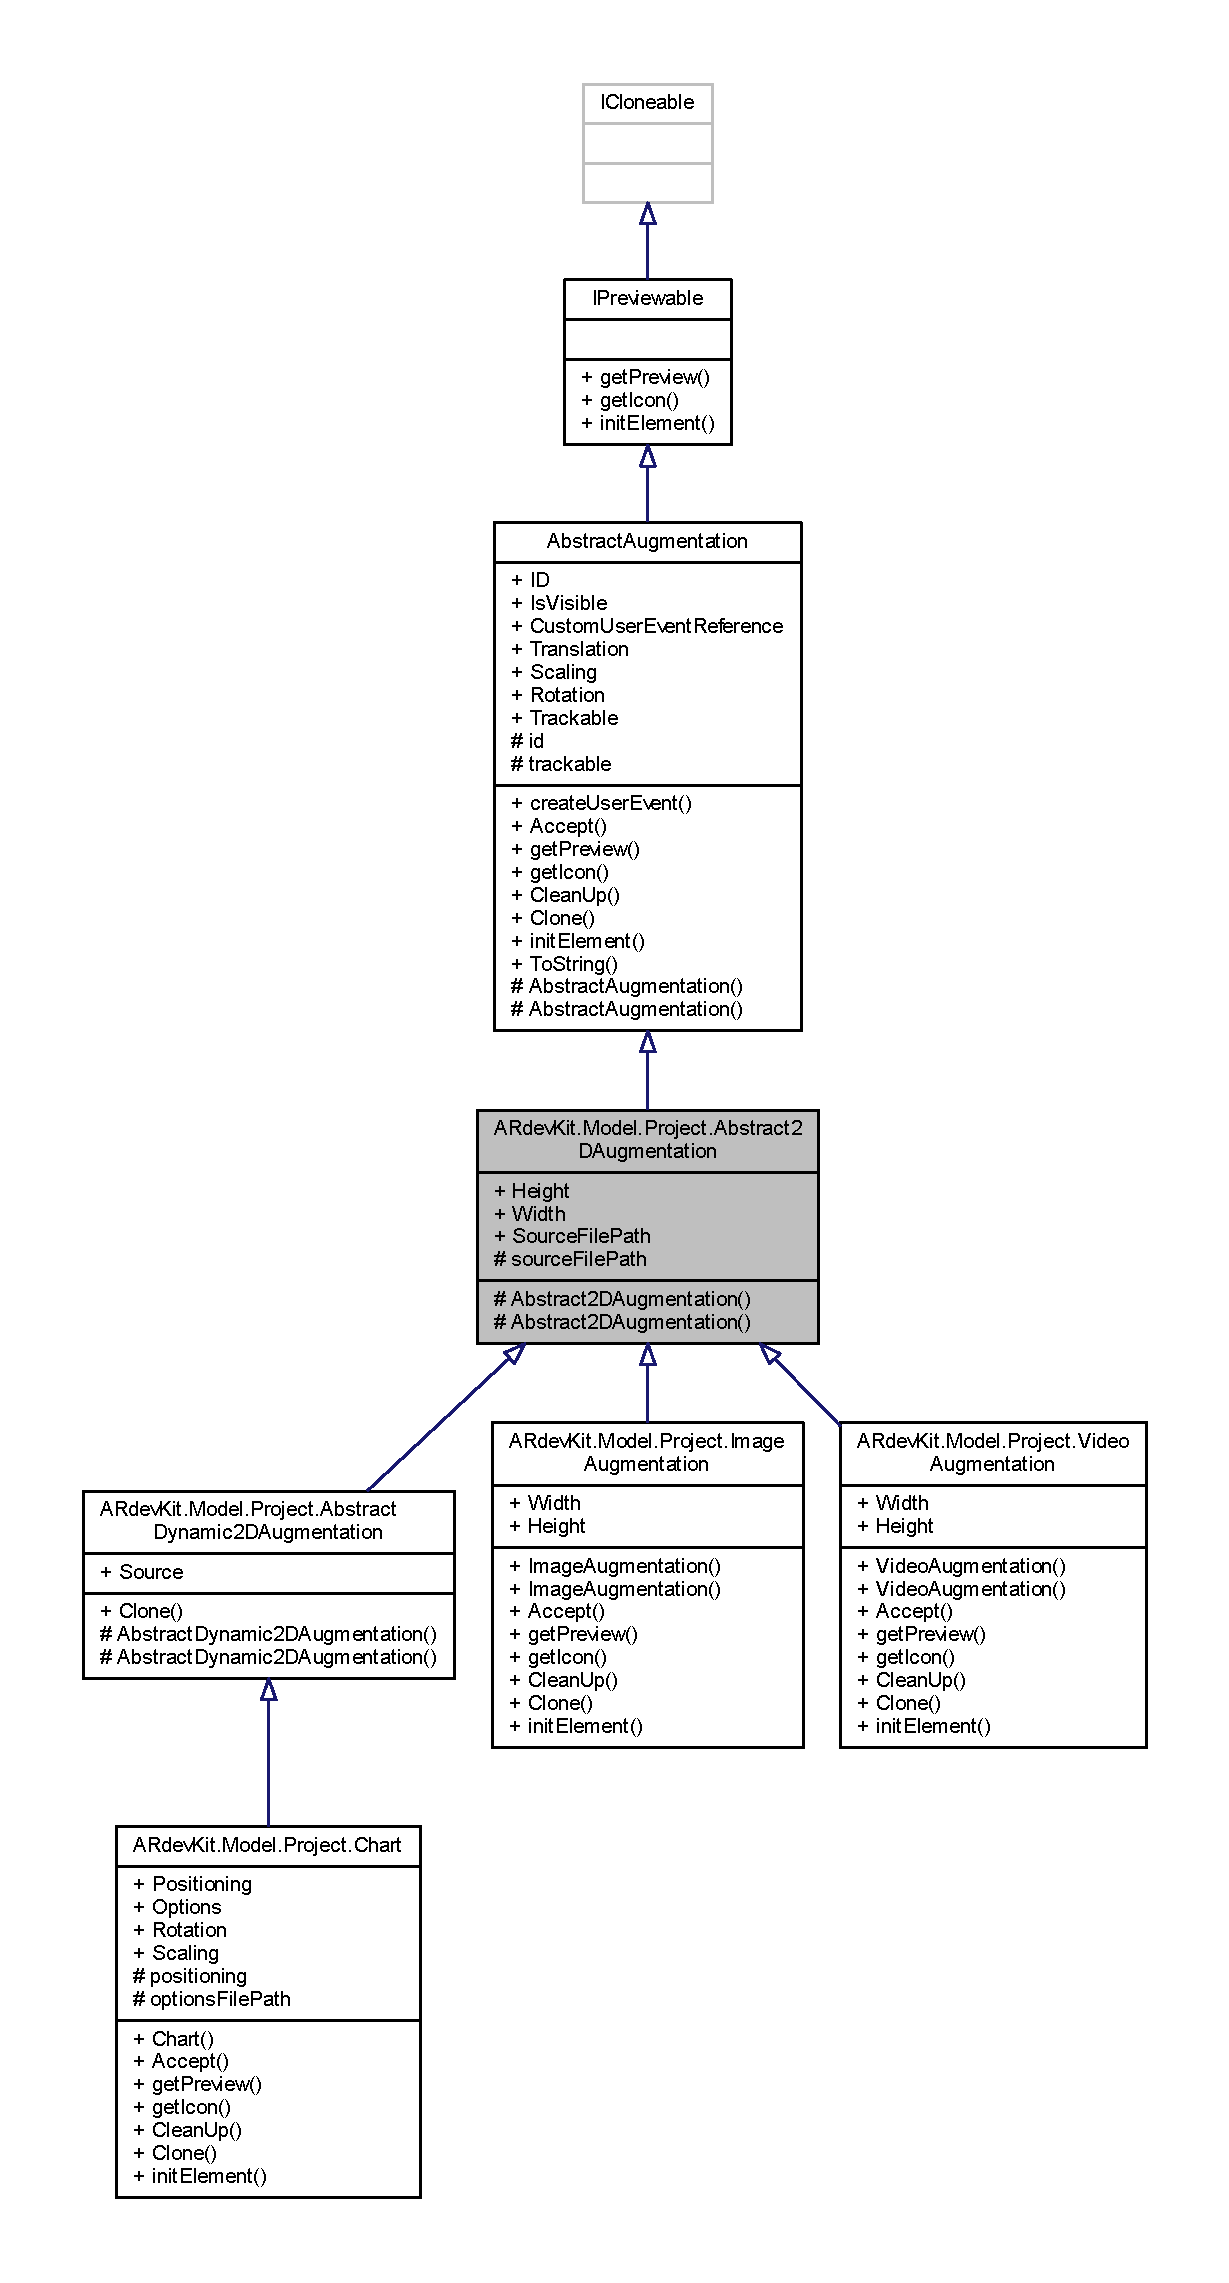
\includegraphics[height=550pt]{class_a_rdev_kit_1_1_model_1_1_project_1_1_abstract2_d_augmentation__inherit__graph}
\end{center}
\end{figure}


Collaboration diagram for A\-Rdev\-Kit.\-Model.\-Project.\-Abstract2\-D\-Augmentation\-:
\nopagebreak
\begin{figure}[H]
\begin{center}
\leavevmode
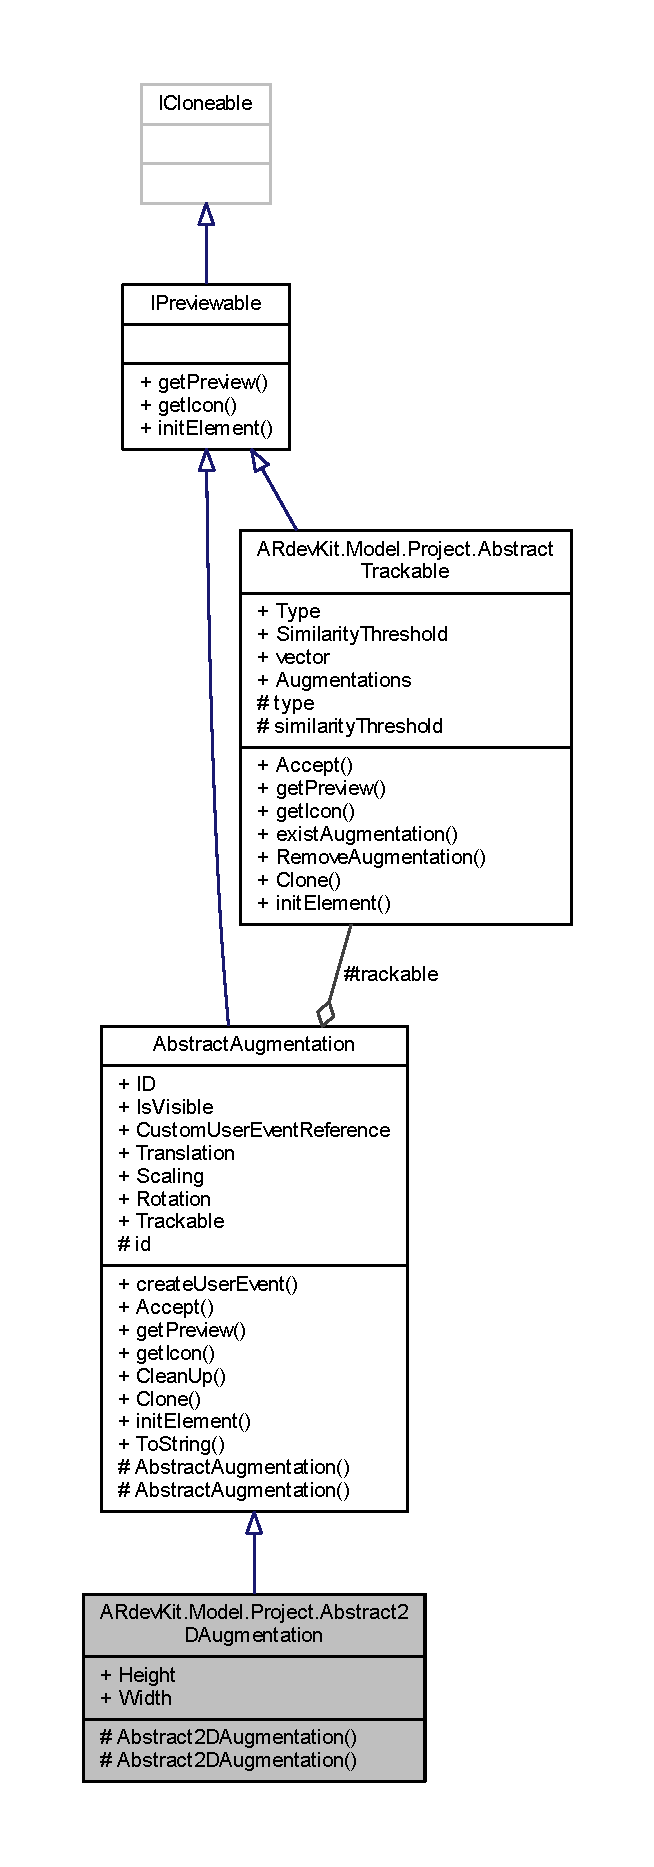
\includegraphics[height=550pt]{class_a_rdev_kit_1_1_model_1_1_project_1_1_abstract2_d_augmentation__coll__graph}
\end{center}
\end{figure}
\subsection*{Protected Member Functions}
\begin{DoxyCompactItemize}
\item 
\hyperlink{class_a_rdev_kit_1_1_model_1_1_project_1_1_abstract2_d_augmentation_adfb4e825f67880c9ec8790a51a60b574}{Abstract2\-D\-Augmentation} ()
\begin{DoxyCompactList}\small\item\em Initializes no new instance of the \hyperlink{class_a_rdev_kit_1_1_model_1_1_project_1_1_abstract2_d_augmentation}{Abstract2\-D\-Augmentation} class, but can be used in inheriting classes. sets height and width = 0 \end{DoxyCompactList}\item 
\hyperlink{class_a_rdev_kit_1_1_model_1_1_project_1_1_abstract2_d_augmentation_a36b71862a4466a4d1942e83e2341cc88}{Abstract2\-D\-Augmentation} (bool is\-Visible, \hyperlink{class_a_rdev_kit_1_1_model_1_1_project_1_1_vector3_d}{Vector3\-D} translation\-Vector, \hyperlink{class_a_rdev_kit_1_1_model_1_1_project_1_1_vector3_d}{Vector3\-D} scaling, \hyperlink{class_a_rdev_kit_1_1_model_1_1_project_1_1_abstract_trackable}{Abstract\-Trackable} \hyperlink{class_a_rdev_kit_1_1_model_1_1_project_1_1_abstract_augmentation_a8d8e3f3c42696008edbfc44d51ba518d}{trackable}, int width, int height)
\begin{DoxyCompactList}\small\item\em constructor, which sets every member of the class as specified, for use from inheriting classes \end{DoxyCompactList}\end{DoxyCompactItemize}
\subsection*{Protected Attributes}
\begin{DoxyCompactItemize}
\item 
string \hyperlink{class_a_rdev_kit_1_1_model_1_1_project_1_1_abstract2_d_augmentation_a9c16053e6d7cd904ad0d9abf823a9b3b}{source\-File\-Path}
\begin{DoxyCompactList}\small\item\em Full pathname of the source file. \end{DoxyCompactList}\end{DoxyCompactItemize}
\subsection*{Properties}
\begin{DoxyCompactItemize}
\item 
int \hyperlink{class_a_rdev_kit_1_1_model_1_1_project_1_1_abstract2_d_augmentation_a14d016654e3824108d413c812f134539}{Height}\hspace{0.3cm}{\ttfamily  \mbox{[}get, set\mbox{]}}
\begin{DoxyCompactList}\small\item\em Gets or sets the height. \end{DoxyCompactList}\item 
int \hyperlink{class_a_rdev_kit_1_1_model_1_1_project_1_1_abstract2_d_augmentation_abbc74c285b3d91be5841ce16473e2cd6}{Width}\hspace{0.3cm}{\ttfamily  \mbox{[}get, set\mbox{]}}
\begin{DoxyCompactList}\small\item\em Gets or sets the width. \end{DoxyCompactList}\item 
string \hyperlink{class_a_rdev_kit_1_1_model_1_1_project_1_1_abstract2_d_augmentation_af2c60054c5ff96c677c84f33c8cb5f9a}{Source\-File\-Path}\hspace{0.3cm}{\ttfamily  \mbox{[}get, set\mbox{]}}
\begin{DoxyCompactList}\small\item\em Gets or sets the full pathname of the image file. \end{DoxyCompactList}\end{DoxyCompactItemize}
\subsection*{Additional Inherited Members}


\subsection{Detailed Description}
Describes an abstract twodimensional augmentation with its additional features height and width. It inherits from \hyperlink{class_a_rdev_kit_1_1_model_1_1_project_1_1_abstract_augmentation}{Abstract\-Augmentation}. 



\subsection{Constructor \& Destructor Documentation}
\hypertarget{class_a_rdev_kit_1_1_model_1_1_project_1_1_abstract2_d_augmentation_adfb4e825f67880c9ec8790a51a60b574}{\index{A\-Rdev\-Kit\-::\-Model\-::\-Project\-::\-Abstract2\-D\-Augmentation@{A\-Rdev\-Kit\-::\-Model\-::\-Project\-::\-Abstract2\-D\-Augmentation}!Abstract2\-D\-Augmentation@{Abstract2\-D\-Augmentation}}
\index{Abstract2\-D\-Augmentation@{Abstract2\-D\-Augmentation}!ARdevKit::Model::Project::Abstract2DAugmentation@{A\-Rdev\-Kit\-::\-Model\-::\-Project\-::\-Abstract2\-D\-Augmentation}}
\subsubsection[{Abstract2\-D\-Augmentation}]{\setlength{\rightskip}{0pt plus 5cm}A\-Rdev\-Kit.\-Model.\-Project.\-Abstract2\-D\-Augmentation.\-Abstract2\-D\-Augmentation (
\begin{DoxyParamCaption}
{}
\end{DoxyParamCaption}
)\hspace{0.3cm}{\ttfamily [protected]}}}\label{class_a_rdev_kit_1_1_model_1_1_project_1_1_abstract2_d_augmentation_adfb4e825f67880c9ec8790a51a60b574}


Initializes no new instance of the \hyperlink{class_a_rdev_kit_1_1_model_1_1_project_1_1_abstract2_d_augmentation}{Abstract2\-D\-Augmentation} class, but can be used in inheriting classes. sets height and width = 0 

\hypertarget{class_a_rdev_kit_1_1_model_1_1_project_1_1_abstract2_d_augmentation_a36b71862a4466a4d1942e83e2341cc88}{\index{A\-Rdev\-Kit\-::\-Model\-::\-Project\-::\-Abstract2\-D\-Augmentation@{A\-Rdev\-Kit\-::\-Model\-::\-Project\-::\-Abstract2\-D\-Augmentation}!Abstract2\-D\-Augmentation@{Abstract2\-D\-Augmentation}}
\index{Abstract2\-D\-Augmentation@{Abstract2\-D\-Augmentation}!ARdevKit::Model::Project::Abstract2DAugmentation@{A\-Rdev\-Kit\-::\-Model\-::\-Project\-::\-Abstract2\-D\-Augmentation}}
\subsubsection[{Abstract2\-D\-Augmentation}]{\setlength{\rightskip}{0pt plus 5cm}A\-Rdev\-Kit.\-Model.\-Project.\-Abstract2\-D\-Augmentation.\-Abstract2\-D\-Augmentation (
\begin{DoxyParamCaption}
\item[{bool}]{is\-Visible, }
\item[{{\bf Vector3\-D}}]{translation\-Vector, }
\item[{{\bf Vector3\-D}}]{scaling, }
\item[{{\bf Abstract\-Trackable}}]{trackable, }
\item[{int}]{width, }
\item[{int}]{height}
\end{DoxyParamCaption}
)\hspace{0.3cm}{\ttfamily [protected]}}}\label{class_a_rdev_kit_1_1_model_1_1_project_1_1_abstract2_d_augmentation_a36b71862a4466a4d1942e83e2341cc88}


constructor, which sets every member of the class as specified, for use from inheriting classes 


\begin{DoxyParams}{Parameters}
{\em is\-Visible} & true if this object is visible. \\
\hline
{\em translation\-Vector} & The translation vector. \\
\hline
{\em scaling} & The scaling. \\
\hline
{\em trackable} & The trackable. \\
\hline
{\em width} & The width. \\
\hline
{\em height} & The height. \\
\hline
\end{DoxyParams}


\subsection{Member Data Documentation}
\hypertarget{class_a_rdev_kit_1_1_model_1_1_project_1_1_abstract2_d_augmentation_a9c16053e6d7cd904ad0d9abf823a9b3b}{\index{A\-Rdev\-Kit\-::\-Model\-::\-Project\-::\-Abstract2\-D\-Augmentation@{A\-Rdev\-Kit\-::\-Model\-::\-Project\-::\-Abstract2\-D\-Augmentation}!source\-File\-Path@{source\-File\-Path}}
\index{source\-File\-Path@{source\-File\-Path}!ARdevKit::Model::Project::Abstract2DAugmentation@{A\-Rdev\-Kit\-::\-Model\-::\-Project\-::\-Abstract2\-D\-Augmentation}}
\subsubsection[{source\-File\-Path}]{\setlength{\rightskip}{0pt plus 5cm}string A\-Rdev\-Kit.\-Model.\-Project.\-Abstract2\-D\-Augmentation.\-source\-File\-Path\hspace{0.3cm}{\ttfamily [protected]}}}\label{class_a_rdev_kit_1_1_model_1_1_project_1_1_abstract2_d_augmentation_a9c16053e6d7cd904ad0d9abf823a9b3b}


Full pathname of the source file. 



\subsection{Property Documentation}
\hypertarget{class_a_rdev_kit_1_1_model_1_1_project_1_1_abstract2_d_augmentation_a14d016654e3824108d413c812f134539}{\index{A\-Rdev\-Kit\-::\-Model\-::\-Project\-::\-Abstract2\-D\-Augmentation@{A\-Rdev\-Kit\-::\-Model\-::\-Project\-::\-Abstract2\-D\-Augmentation}!Height@{Height}}
\index{Height@{Height}!ARdevKit::Model::Project::Abstract2DAugmentation@{A\-Rdev\-Kit\-::\-Model\-::\-Project\-::\-Abstract2\-D\-Augmentation}}
\subsubsection[{Height}]{\setlength{\rightskip}{0pt plus 5cm}int A\-Rdev\-Kit.\-Model.\-Project.\-Abstract2\-D\-Augmentation.\-Height\hspace{0.3cm}{\ttfamily [get]}, {\ttfamily [set]}}}\label{class_a_rdev_kit_1_1_model_1_1_project_1_1_abstract2_d_augmentation_a14d016654e3824108d413c812f134539}


Gets or sets the height. 

The height, in mm. \hypertarget{class_a_rdev_kit_1_1_model_1_1_project_1_1_abstract2_d_augmentation_af2c60054c5ff96c677c84f33c8cb5f9a}{\index{A\-Rdev\-Kit\-::\-Model\-::\-Project\-::\-Abstract2\-D\-Augmentation@{A\-Rdev\-Kit\-::\-Model\-::\-Project\-::\-Abstract2\-D\-Augmentation}!Source\-File\-Path@{Source\-File\-Path}}
\index{Source\-File\-Path@{Source\-File\-Path}!ARdevKit::Model::Project::Abstract2DAugmentation@{A\-Rdev\-Kit\-::\-Model\-::\-Project\-::\-Abstract2\-D\-Augmentation}}
\subsubsection[{Source\-File\-Path}]{\setlength{\rightskip}{0pt plus 5cm}string A\-Rdev\-Kit.\-Model.\-Project.\-Abstract2\-D\-Augmentation.\-Source\-File\-Path\hspace{0.3cm}{\ttfamily [get]}, {\ttfamily [set]}}}\label{class_a_rdev_kit_1_1_model_1_1_project_1_1_abstract2_d_augmentation_af2c60054c5ff96c677c84f33c8cb5f9a}


Gets or sets the full pathname of the image file. 

The full pathname of the image file. \hypertarget{class_a_rdev_kit_1_1_model_1_1_project_1_1_abstract2_d_augmentation_abbc74c285b3d91be5841ce16473e2cd6}{\index{A\-Rdev\-Kit\-::\-Model\-::\-Project\-::\-Abstract2\-D\-Augmentation@{A\-Rdev\-Kit\-::\-Model\-::\-Project\-::\-Abstract2\-D\-Augmentation}!Width@{Width}}
\index{Width@{Width}!ARdevKit::Model::Project::Abstract2DAugmentation@{A\-Rdev\-Kit\-::\-Model\-::\-Project\-::\-Abstract2\-D\-Augmentation}}
\subsubsection[{Width}]{\setlength{\rightskip}{0pt plus 5cm}int A\-Rdev\-Kit.\-Model.\-Project.\-Abstract2\-D\-Augmentation.\-Width\hspace{0.3cm}{\ttfamily [get]}, {\ttfamily [set]}}}\label{class_a_rdev_kit_1_1_model_1_1_project_1_1_abstract2_d_augmentation_abbc74c285b3d91be5841ce16473e2cd6}


Gets or sets the width. 

The width, in mm. 
\hypertarget{class_a_rdev_kit_1_1_model_1_1_project_1_1_abstract2_d_trackable}{\section{A\-Rdev\-Kit.\-Model.\-Project.\-Abstract2\-D\-Trackable Class Reference}
\label{class_a_rdev_kit_1_1_model_1_1_project_1_1_abstract2_d_trackable}\index{A\-Rdev\-Kit.\-Model.\-Project.\-Abstract2\-D\-Trackable@{A\-Rdev\-Kit.\-Model.\-Project.\-Abstract2\-D\-Trackable}}
}


An \hyperlink{class_a_rdev_kit_1_1_model_1_1_project_1_1_abstract2_d_trackable}{Abstract2\-D\-Trackable} is a two-\/dimensional trackable image, that can be tracked by the metaio S\-D\-K.  




Inheritance diagram for A\-Rdev\-Kit.\-Model.\-Project.\-Abstract2\-D\-Trackable\-:
\nopagebreak
\begin{figure}[H]
\begin{center}
\leavevmode
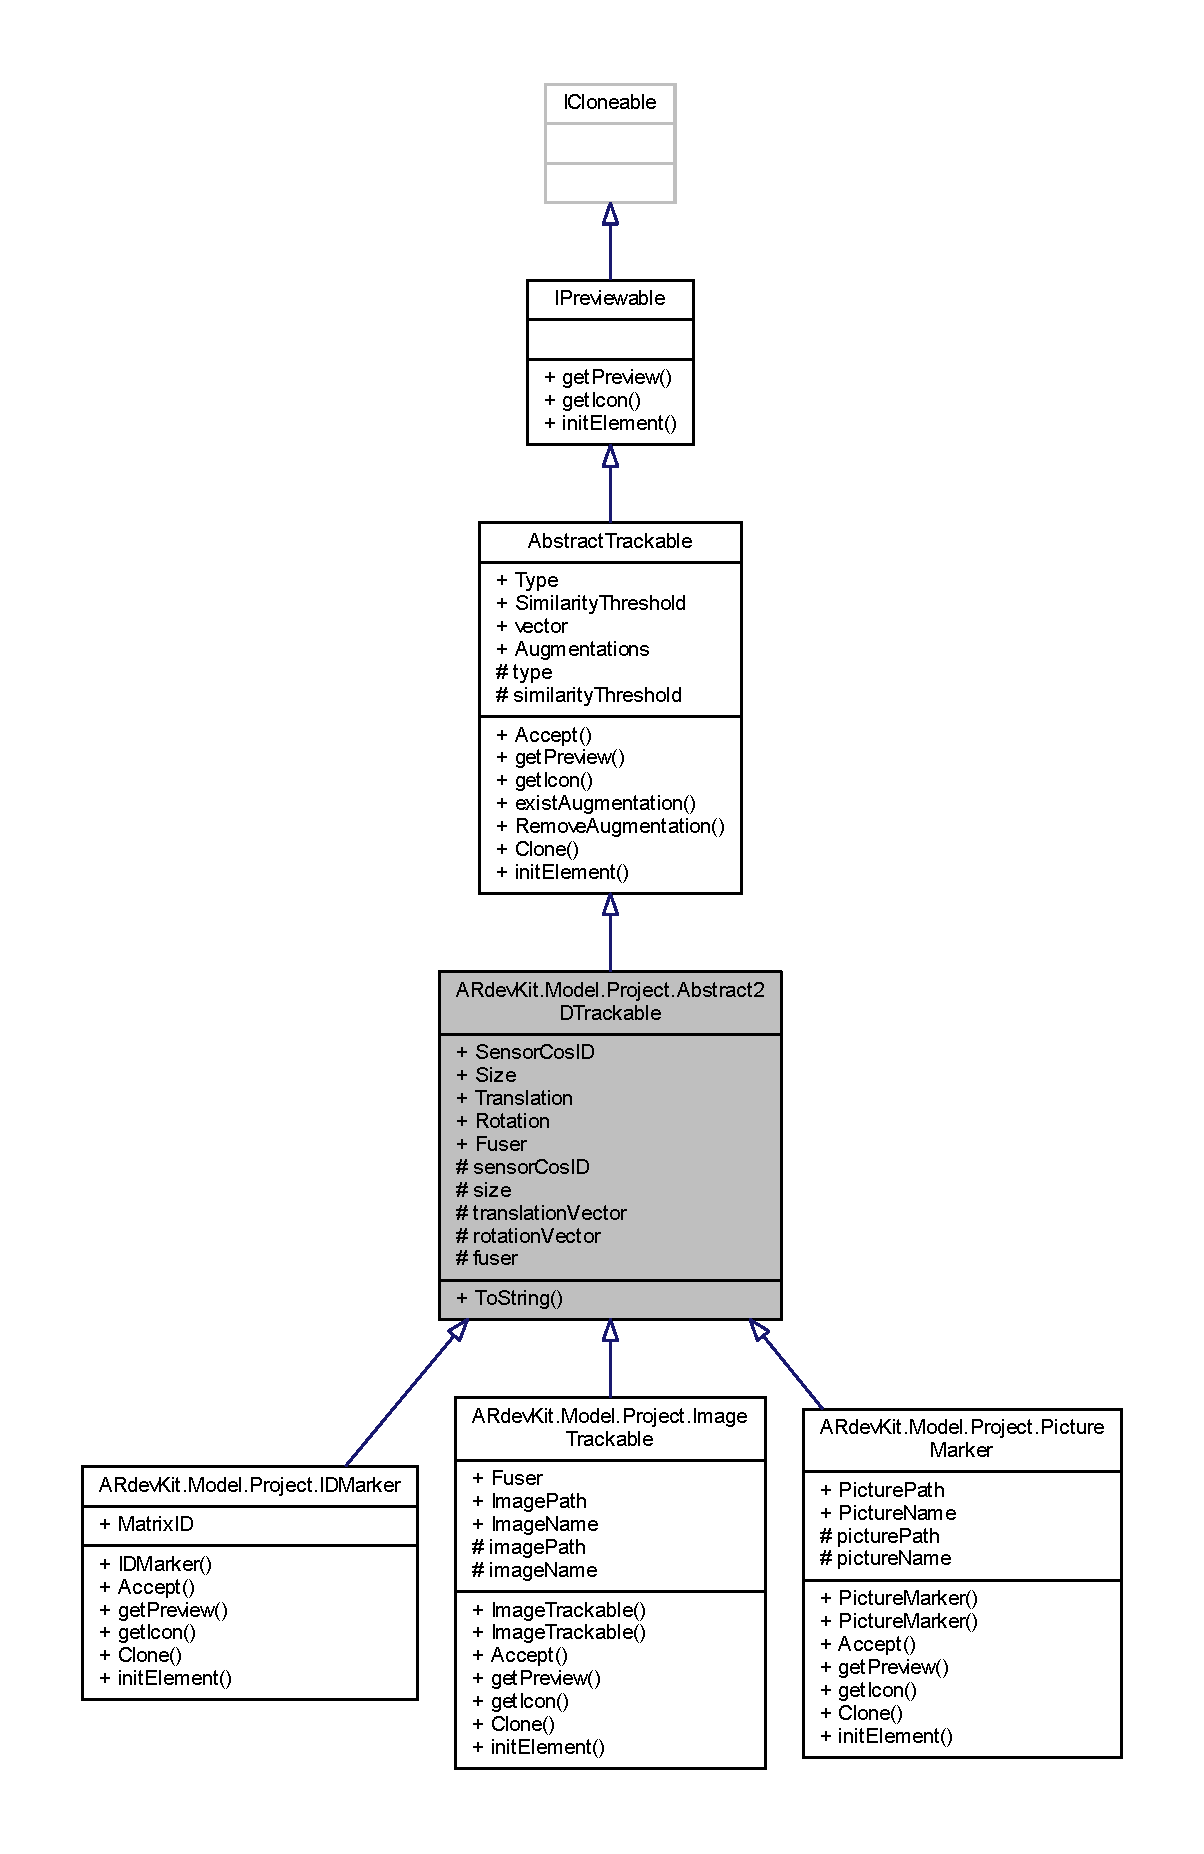
\includegraphics[width=350pt]{class_a_rdev_kit_1_1_model_1_1_project_1_1_abstract2_d_trackable__inherit__graph}
\end{center}
\end{figure}


Collaboration diagram for A\-Rdev\-Kit.\-Model.\-Project.\-Abstract2\-D\-Trackable\-:
\nopagebreak
\begin{figure}[H]
\begin{center}
\leavevmode
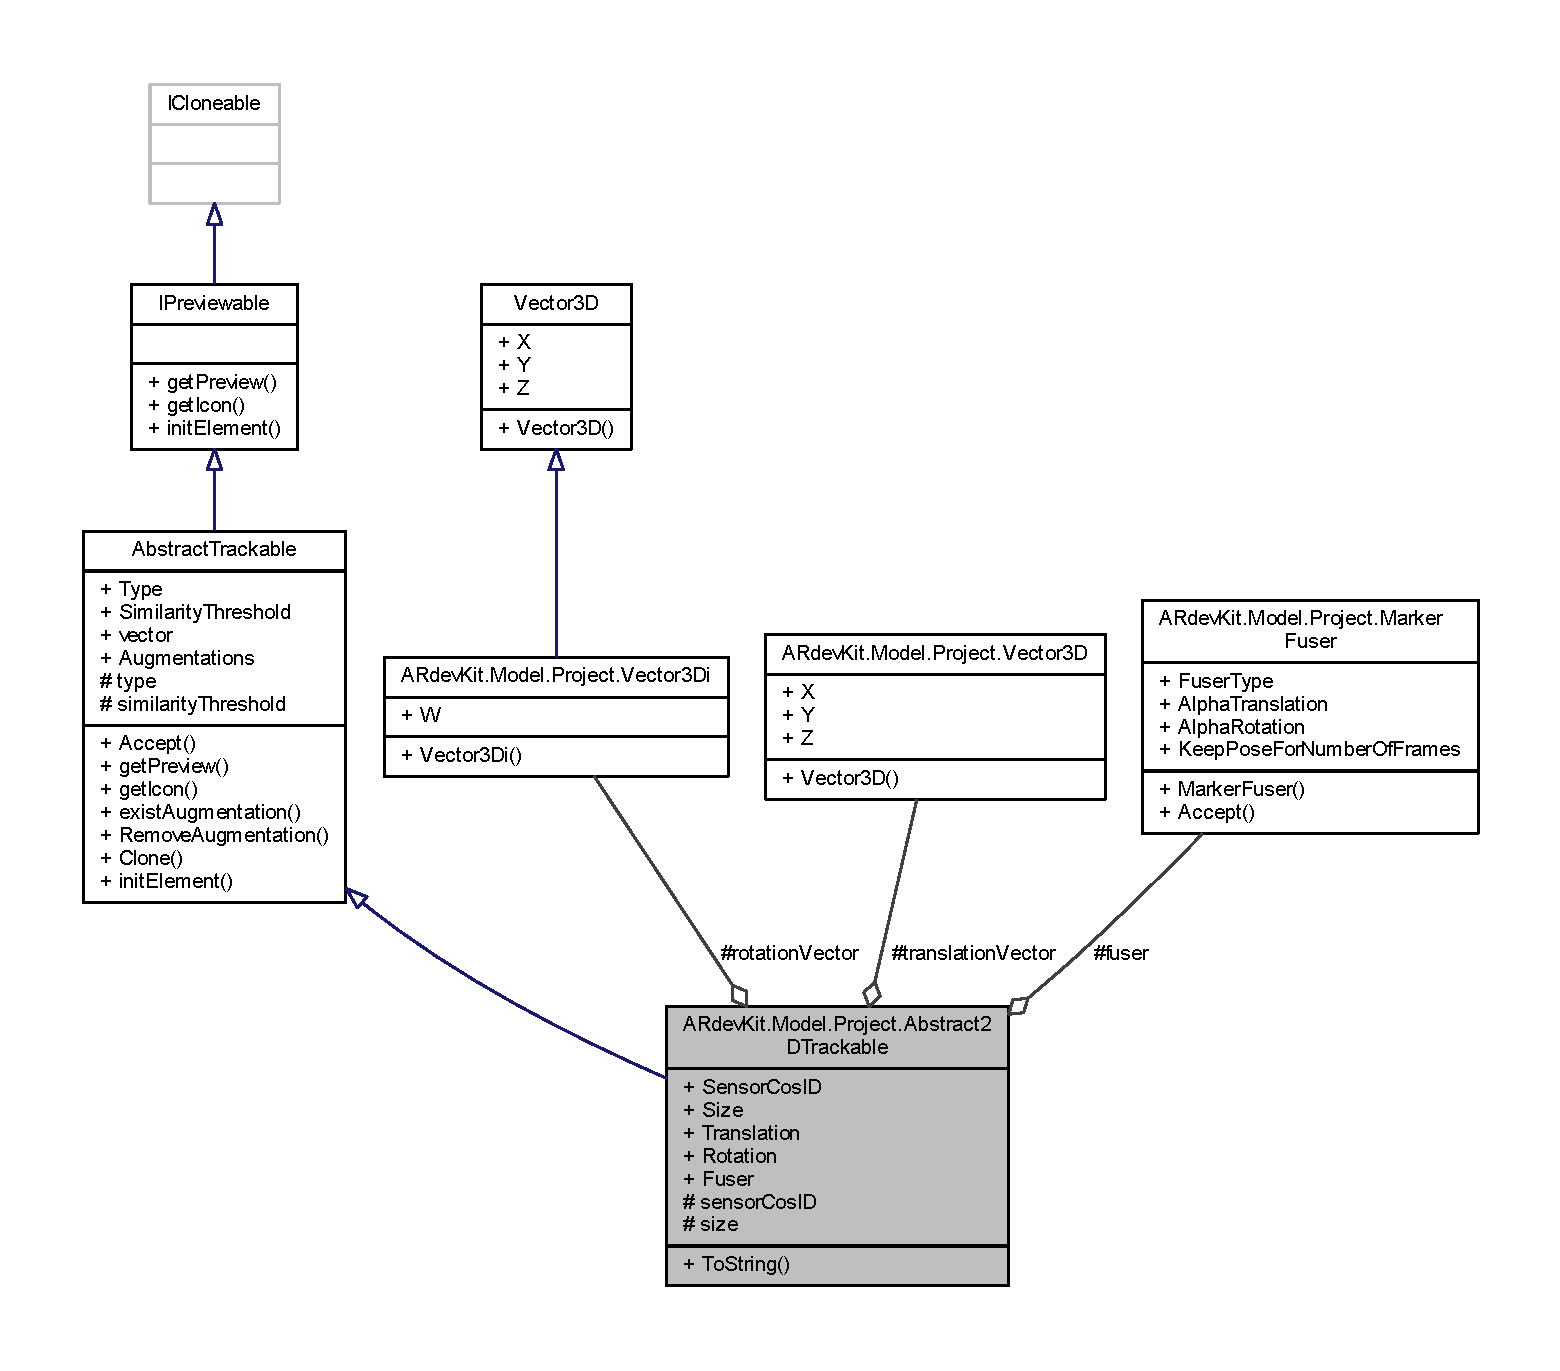
\includegraphics[width=350pt]{class_a_rdev_kit_1_1_model_1_1_project_1_1_abstract2_d_trackable__coll__graph}
\end{center}
\end{figure}
\subsection*{Public Member Functions}
\begin{DoxyCompactItemize}
\item 
override string \hyperlink{class_a_rdev_kit_1_1_model_1_1_project_1_1_abstract2_d_trackable_ac836d823c247762a615f432375d943c2}{To\-String} ()
\begin{DoxyCompactList}\small\item\em Gibt eine Zeichenfolge zurück, die das aktuelle Objekt darstellt. \end{DoxyCompactList}\end{DoxyCompactItemize}
\subsection*{Protected Attributes}
\begin{DoxyCompactItemize}
\item 
string \hyperlink{class_a_rdev_kit_1_1_model_1_1_project_1_1_abstract2_d_trackable_ac965f78edc7135b60377d14acbe6d358}{sensor\-Cos\-I\-D}
\begin{DoxyCompactList}\small\item\em The sensor cos identifier, used by A\-R\-E\-L to specify the Tracking\-Data \end{DoxyCompactList}\item 
int \hyperlink{class_a_rdev_kit_1_1_model_1_1_project_1_1_abstract2_d_trackable_a3ef9116db48c612d3428126786516e81}{size}
\begin{DoxyCompactList}\small\item\em The size of the Marker in mm \end{DoxyCompactList}\item 
\hyperlink{class_a_rdev_kit_1_1_model_1_1_project_1_1_vector3_d}{Vector3\-D} \hyperlink{class_a_rdev_kit_1_1_model_1_1_project_1_1_abstract2_d_trackable_a5d6e8cbc9efc6da689e3537d334fec37}{translation\-Vector}
\begin{DoxyCompactList}\small\item\em Vector to describe the position on the Preview\-Panel, and later to position it on the coordinatesystem given in A\-R\-E\-L. \end{DoxyCompactList}\item 
\hyperlink{class_a_rdev_kit_1_1_model_1_1_project_1_1_vector3_di}{Vector3\-Di} \hyperlink{class_a_rdev_kit_1_1_model_1_1_project_1_1_abstract2_d_trackable_a85997ab052b01f3680d47d199b4551a0}{rotation\-Vector}
\begin{DoxyCompactList}\small\item\em Vector, to describe the rotation of the \hyperlink{class_a_rdev_kit_1_1_model_1_1_project_1_1_abstract_augmentation}{Abstract\-Augmentation} in x, y and z direction. w is used for Tracking\-File Offset in A\-R\-E\-L. \end{DoxyCompactList}\item 
\hyperlink{class_a_rdev_kit_1_1_model_1_1_project_1_1_marker_fuser}{Marker\-Fuser} \hyperlink{class_a_rdev_kit_1_1_model_1_1_project_1_1_abstract2_d_trackable_a8ebdec7d02359310504e15f3a9852c04}{fuser}
\begin{DoxyCompactList}\small\item\em Describes how different elements are combined and connected in A\-R\-E\-L. \end{DoxyCompactList}\end{DoxyCompactItemize}
\subsection*{Properties}
\begin{DoxyCompactItemize}
\item 
string \hyperlink{class_a_rdev_kit_1_1_model_1_1_project_1_1_abstract2_d_trackable_a9578380939f19267cc7372ca19ff936f}{Sensor\-Cos\-I\-D}\hspace{0.3cm}{\ttfamily  \mbox{[}get, set\mbox{]}}
\begin{DoxyCompactList}\small\item\em Gets or sets the sensor cos identifier. \end{DoxyCompactList}\item 
int \hyperlink{class_a_rdev_kit_1_1_model_1_1_project_1_1_abstract2_d_trackable_a0c9a459cf25e74c8173564d476021c9a}{Size}\hspace{0.3cm}{\ttfamily  \mbox{[}get, set\mbox{]}}
\begin{DoxyCompactList}\small\item\em Gets or sets the size. \end{DoxyCompactList}\item 
\hyperlink{class_a_rdev_kit_1_1_model_1_1_project_1_1_vector3_d}{Vector3\-D} \hyperlink{class_a_rdev_kit_1_1_model_1_1_project_1_1_abstract2_d_trackable_acbb38387d30cb1239814606b54099bb3}{Translation}\hspace{0.3cm}{\ttfamily  \mbox{[}get, set\mbox{]}}
\begin{DoxyCompactList}\small\item\em Get or set the position of the \hyperlink{class_a_rdev_kit_1_1_model_1_1_project_1_1_abstract_augmentation}{Abstract\-Augmentation}. \end{DoxyCompactList}\item 
\hyperlink{class_a_rdev_kit_1_1_model_1_1_project_1_1_vector3_di}{Vector3\-Di} \hyperlink{class_a_rdev_kit_1_1_model_1_1_project_1_1_abstract2_d_trackable_a12ba493972e7d277e8f67294beb70355}{Rotation}\hspace{0.3cm}{\ttfamily  \mbox{[}get, set\mbox{]}}
\begin{DoxyCompactList}\small\item\em gets or sets the Vector \end{DoxyCompactList}\item 
\hyperlink{class_a_rdev_kit_1_1_model_1_1_project_1_1_marker_fuser}{Marker\-Fuser} \hyperlink{class_a_rdev_kit_1_1_model_1_1_project_1_1_abstract2_d_trackable_a98e3270dac234f5acd6054707f4c1964}{Fuser}\hspace{0.3cm}{\ttfamily  \mbox{[}get, set\mbox{]}}
\begin{DoxyCompactList}\small\item\em Gets or sets the fuser. Is not Browsable, therefore not editable in the Property\-Panel \end{DoxyCompactList}\end{DoxyCompactItemize}


\subsection{Detailed Description}
An \hyperlink{class_a_rdev_kit_1_1_model_1_1_project_1_1_abstract2_d_trackable}{Abstract2\-D\-Trackable} is a two-\/dimensional trackable image, that can be tracked by the metaio S\-D\-K. 



\subsection{Member Function Documentation}
\hypertarget{class_a_rdev_kit_1_1_model_1_1_project_1_1_abstract2_d_trackable_ac836d823c247762a615f432375d943c2}{\index{A\-Rdev\-Kit\-::\-Model\-::\-Project\-::\-Abstract2\-D\-Trackable@{A\-Rdev\-Kit\-::\-Model\-::\-Project\-::\-Abstract2\-D\-Trackable}!To\-String@{To\-String}}
\index{To\-String@{To\-String}!ARdevKit::Model::Project::Abstract2DTrackable@{A\-Rdev\-Kit\-::\-Model\-::\-Project\-::\-Abstract2\-D\-Trackable}}
\subsubsection[{To\-String}]{\setlength{\rightskip}{0pt plus 5cm}override string A\-Rdev\-Kit.\-Model.\-Project.\-Abstract2\-D\-Trackable.\-To\-String (
\begin{DoxyParamCaption}
{}
\end{DoxyParamCaption}
)}}\label{class_a_rdev_kit_1_1_model_1_1_project_1_1_abstract2_d_trackable_ac836d823c247762a615f432375d943c2}


Gibt eine Zeichenfolge zurück, die das aktuelle Objekt darstellt. 

Robin, 14.\-01.\-2014. 

\begin{DoxyReturn}{Returns}
Eine Zeichenfolge, die das aktuelle Objekt darstellt. 
\end{DoxyReturn}


\subsection{Member Data Documentation}
\hypertarget{class_a_rdev_kit_1_1_model_1_1_project_1_1_abstract2_d_trackable_a8ebdec7d02359310504e15f3a9852c04}{\index{A\-Rdev\-Kit\-::\-Model\-::\-Project\-::\-Abstract2\-D\-Trackable@{A\-Rdev\-Kit\-::\-Model\-::\-Project\-::\-Abstract2\-D\-Trackable}!fuser@{fuser}}
\index{fuser@{fuser}!ARdevKit::Model::Project::Abstract2DTrackable@{A\-Rdev\-Kit\-::\-Model\-::\-Project\-::\-Abstract2\-D\-Trackable}}
\subsubsection[{fuser}]{\setlength{\rightskip}{0pt plus 5cm}{\bf Marker\-Fuser} A\-Rdev\-Kit.\-Model.\-Project.\-Abstract2\-D\-Trackable.\-fuser\hspace{0.3cm}{\ttfamily [protected]}}}\label{class_a_rdev_kit_1_1_model_1_1_project_1_1_abstract2_d_trackable_a8ebdec7d02359310504e15f3a9852c04}


Describes how different elements are combined and connected in A\-R\-E\-L. 

\hypertarget{class_a_rdev_kit_1_1_model_1_1_project_1_1_abstract2_d_trackable_a85997ab052b01f3680d47d199b4551a0}{\index{A\-Rdev\-Kit\-::\-Model\-::\-Project\-::\-Abstract2\-D\-Trackable@{A\-Rdev\-Kit\-::\-Model\-::\-Project\-::\-Abstract2\-D\-Trackable}!rotation\-Vector@{rotation\-Vector}}
\index{rotation\-Vector@{rotation\-Vector}!ARdevKit::Model::Project::Abstract2DTrackable@{A\-Rdev\-Kit\-::\-Model\-::\-Project\-::\-Abstract2\-D\-Trackable}}
\subsubsection[{rotation\-Vector}]{\setlength{\rightskip}{0pt plus 5cm}{\bf Vector3\-Di} A\-Rdev\-Kit.\-Model.\-Project.\-Abstract2\-D\-Trackable.\-rotation\-Vector\hspace{0.3cm}{\ttfamily [protected]}}}\label{class_a_rdev_kit_1_1_model_1_1_project_1_1_abstract2_d_trackable_a85997ab052b01f3680d47d199b4551a0}


Vector, to describe the rotation of the \hyperlink{class_a_rdev_kit_1_1_model_1_1_project_1_1_abstract_augmentation}{Abstract\-Augmentation} in x, y and z direction. w is used for Tracking\-File Offset in A\-R\-E\-L. 

\hypertarget{class_a_rdev_kit_1_1_model_1_1_project_1_1_abstract2_d_trackable_ac965f78edc7135b60377d14acbe6d358}{\index{A\-Rdev\-Kit\-::\-Model\-::\-Project\-::\-Abstract2\-D\-Trackable@{A\-Rdev\-Kit\-::\-Model\-::\-Project\-::\-Abstract2\-D\-Trackable}!sensor\-Cos\-I\-D@{sensor\-Cos\-I\-D}}
\index{sensor\-Cos\-I\-D@{sensor\-Cos\-I\-D}!ARdevKit::Model::Project::Abstract2DTrackable@{A\-Rdev\-Kit\-::\-Model\-::\-Project\-::\-Abstract2\-D\-Trackable}}
\subsubsection[{sensor\-Cos\-I\-D}]{\setlength{\rightskip}{0pt plus 5cm}string A\-Rdev\-Kit.\-Model.\-Project.\-Abstract2\-D\-Trackable.\-sensor\-Cos\-I\-D\hspace{0.3cm}{\ttfamily [protected]}}}\label{class_a_rdev_kit_1_1_model_1_1_project_1_1_abstract2_d_trackable_ac965f78edc7135b60377d14acbe6d358}


The sensor cos identifier, used by A\-R\-E\-L to specify the Tracking\-Data 

\hypertarget{class_a_rdev_kit_1_1_model_1_1_project_1_1_abstract2_d_trackable_a3ef9116db48c612d3428126786516e81}{\index{A\-Rdev\-Kit\-::\-Model\-::\-Project\-::\-Abstract2\-D\-Trackable@{A\-Rdev\-Kit\-::\-Model\-::\-Project\-::\-Abstract2\-D\-Trackable}!size@{size}}
\index{size@{size}!ARdevKit::Model::Project::Abstract2DTrackable@{A\-Rdev\-Kit\-::\-Model\-::\-Project\-::\-Abstract2\-D\-Trackable}}
\subsubsection[{size}]{\setlength{\rightskip}{0pt plus 5cm}int A\-Rdev\-Kit.\-Model.\-Project.\-Abstract2\-D\-Trackable.\-size\hspace{0.3cm}{\ttfamily [protected]}}}\label{class_a_rdev_kit_1_1_model_1_1_project_1_1_abstract2_d_trackable_a3ef9116db48c612d3428126786516e81}


The size of the Marker in mm 

\hypertarget{class_a_rdev_kit_1_1_model_1_1_project_1_1_abstract2_d_trackable_a5d6e8cbc9efc6da689e3537d334fec37}{\index{A\-Rdev\-Kit\-::\-Model\-::\-Project\-::\-Abstract2\-D\-Trackable@{A\-Rdev\-Kit\-::\-Model\-::\-Project\-::\-Abstract2\-D\-Trackable}!translation\-Vector@{translation\-Vector}}
\index{translation\-Vector@{translation\-Vector}!ARdevKit::Model::Project::Abstract2DTrackable@{A\-Rdev\-Kit\-::\-Model\-::\-Project\-::\-Abstract2\-D\-Trackable}}
\subsubsection[{translation\-Vector}]{\setlength{\rightskip}{0pt plus 5cm}{\bf Vector3\-D} A\-Rdev\-Kit.\-Model.\-Project.\-Abstract2\-D\-Trackable.\-translation\-Vector\hspace{0.3cm}{\ttfamily [protected]}}}\label{class_a_rdev_kit_1_1_model_1_1_project_1_1_abstract2_d_trackable_a5d6e8cbc9efc6da689e3537d334fec37}


Vector to describe the position on the Preview\-Panel, and later to position it on the coordinatesystem given in A\-R\-E\-L. 



\subsection{Property Documentation}
\hypertarget{class_a_rdev_kit_1_1_model_1_1_project_1_1_abstract2_d_trackable_a98e3270dac234f5acd6054707f4c1964}{\index{A\-Rdev\-Kit\-::\-Model\-::\-Project\-::\-Abstract2\-D\-Trackable@{A\-Rdev\-Kit\-::\-Model\-::\-Project\-::\-Abstract2\-D\-Trackable}!Fuser@{Fuser}}
\index{Fuser@{Fuser}!ARdevKit::Model::Project::Abstract2DTrackable@{A\-Rdev\-Kit\-::\-Model\-::\-Project\-::\-Abstract2\-D\-Trackable}}
\subsubsection[{Fuser}]{\setlength{\rightskip}{0pt plus 5cm}{\bf Marker\-Fuser} A\-Rdev\-Kit.\-Model.\-Project.\-Abstract2\-D\-Trackable.\-Fuser\hspace{0.3cm}{\ttfamily [get]}, {\ttfamily [set]}}}\label{class_a_rdev_kit_1_1_model_1_1_project_1_1_abstract2_d_trackable_a98e3270dac234f5acd6054707f4c1964}


Gets or sets the fuser. Is not Browsable, therefore not editable in the Property\-Panel 

The fuser. \hypertarget{class_a_rdev_kit_1_1_model_1_1_project_1_1_abstract2_d_trackable_a12ba493972e7d277e8f67294beb70355}{\index{A\-Rdev\-Kit\-::\-Model\-::\-Project\-::\-Abstract2\-D\-Trackable@{A\-Rdev\-Kit\-::\-Model\-::\-Project\-::\-Abstract2\-D\-Trackable}!Rotation@{Rotation}}
\index{Rotation@{Rotation}!ARdevKit::Model::Project::Abstract2DTrackable@{A\-Rdev\-Kit\-::\-Model\-::\-Project\-::\-Abstract2\-D\-Trackable}}
\subsubsection[{Rotation}]{\setlength{\rightskip}{0pt plus 5cm}{\bf Vector3\-Di} A\-Rdev\-Kit.\-Model.\-Project.\-Abstract2\-D\-Trackable.\-Rotation\hspace{0.3cm}{\ttfamily [get]}, {\ttfamily [set]}}}\label{class_a_rdev_kit_1_1_model_1_1_project_1_1_abstract2_d_trackable_a12ba493972e7d277e8f67294beb70355}


gets or sets the Vector 

\hypertarget{class_a_rdev_kit_1_1_model_1_1_project_1_1_abstract2_d_trackable_a9578380939f19267cc7372ca19ff936f}{\index{A\-Rdev\-Kit\-::\-Model\-::\-Project\-::\-Abstract2\-D\-Trackable@{A\-Rdev\-Kit\-::\-Model\-::\-Project\-::\-Abstract2\-D\-Trackable}!Sensor\-Cos\-I\-D@{Sensor\-Cos\-I\-D}}
\index{Sensor\-Cos\-I\-D@{Sensor\-Cos\-I\-D}!ARdevKit::Model::Project::Abstract2DTrackable@{A\-Rdev\-Kit\-::\-Model\-::\-Project\-::\-Abstract2\-D\-Trackable}}
\subsubsection[{Sensor\-Cos\-I\-D}]{\setlength{\rightskip}{0pt plus 5cm}string A\-Rdev\-Kit.\-Model.\-Project.\-Abstract2\-D\-Trackable.\-Sensor\-Cos\-I\-D\hspace{0.3cm}{\ttfamily [get]}, {\ttfamily [set]}}}\label{class_a_rdev_kit_1_1_model_1_1_project_1_1_abstract2_d_trackable_a9578380939f19267cc7372ca19ff936f}


Gets or sets the sensor cos identifier. 

\hypertarget{class_a_rdev_kit_1_1_model_1_1_project_1_1_abstract2_d_trackable_a0c9a459cf25e74c8173564d476021c9a}{\index{A\-Rdev\-Kit\-::\-Model\-::\-Project\-::\-Abstract2\-D\-Trackable@{A\-Rdev\-Kit\-::\-Model\-::\-Project\-::\-Abstract2\-D\-Trackable}!Size@{Size}}
\index{Size@{Size}!ARdevKit::Model::Project::Abstract2DTrackable@{A\-Rdev\-Kit\-::\-Model\-::\-Project\-::\-Abstract2\-D\-Trackable}}
\subsubsection[{Size}]{\setlength{\rightskip}{0pt plus 5cm}int A\-Rdev\-Kit.\-Model.\-Project.\-Abstract2\-D\-Trackable.\-Size\hspace{0.3cm}{\ttfamily [get]}, {\ttfamily [set]}}}\label{class_a_rdev_kit_1_1_model_1_1_project_1_1_abstract2_d_trackable_a0c9a459cf25e74c8173564d476021c9a}


Gets or sets the size. 

\hypertarget{class_a_rdev_kit_1_1_model_1_1_project_1_1_abstract2_d_trackable_acbb38387d30cb1239814606b54099bb3}{\index{A\-Rdev\-Kit\-::\-Model\-::\-Project\-::\-Abstract2\-D\-Trackable@{A\-Rdev\-Kit\-::\-Model\-::\-Project\-::\-Abstract2\-D\-Trackable}!Translation@{Translation}}
\index{Translation@{Translation}!ARdevKit::Model::Project::Abstract2DTrackable@{A\-Rdev\-Kit\-::\-Model\-::\-Project\-::\-Abstract2\-D\-Trackable}}
\subsubsection[{Translation}]{\setlength{\rightskip}{0pt plus 5cm}{\bf Vector3\-D} A\-Rdev\-Kit.\-Model.\-Project.\-Abstract2\-D\-Trackable.\-Translation\hspace{0.3cm}{\ttfamily [get]}, {\ttfamily [set]}}}\label{class_a_rdev_kit_1_1_model_1_1_project_1_1_abstract2_d_trackable_acbb38387d30cb1239814606b54099bb3}


Get or set the position of the \hyperlink{class_a_rdev_kit_1_1_model_1_1_project_1_1_abstract_augmentation}{Abstract\-Augmentation}. 


\hypertarget{class_a_rdev_kit_1_1_model_1_1_project_1_1_abstract_augmentation}{\section{A\-Rdev\-Kit.\-Model.\-Project.\-Abstract\-Augmentation Class Reference}
\label{class_a_rdev_kit_1_1_model_1_1_project_1_1_abstract_augmentation}\index{A\-Rdev\-Kit.\-Model.\-Project.\-Abstract\-Augmentation@{A\-Rdev\-Kit.\-Model.\-Project.\-Abstract\-Augmentation}}
}


describes an \hyperlink{class_a_rdev_kit_1_1_model_1_1_project_1_1_abstract_augmentation}{Abstract\-Augmentation}, which is bound to a certain \hyperlink{class_a_rdev_kit_1_1_model_1_1_project_1_1_abstract_trackable}{Abstract\-Trackable}. is \hyperlink{interface_a_rdev_kit_1_1_model_1_1_project_1_1_i_previewable}{I\-Previewable}  




Inheritance diagram for A\-Rdev\-Kit.\-Model.\-Project.\-Abstract\-Augmentation\-:
\nopagebreak
\begin{figure}[H]
\begin{center}
\leavevmode
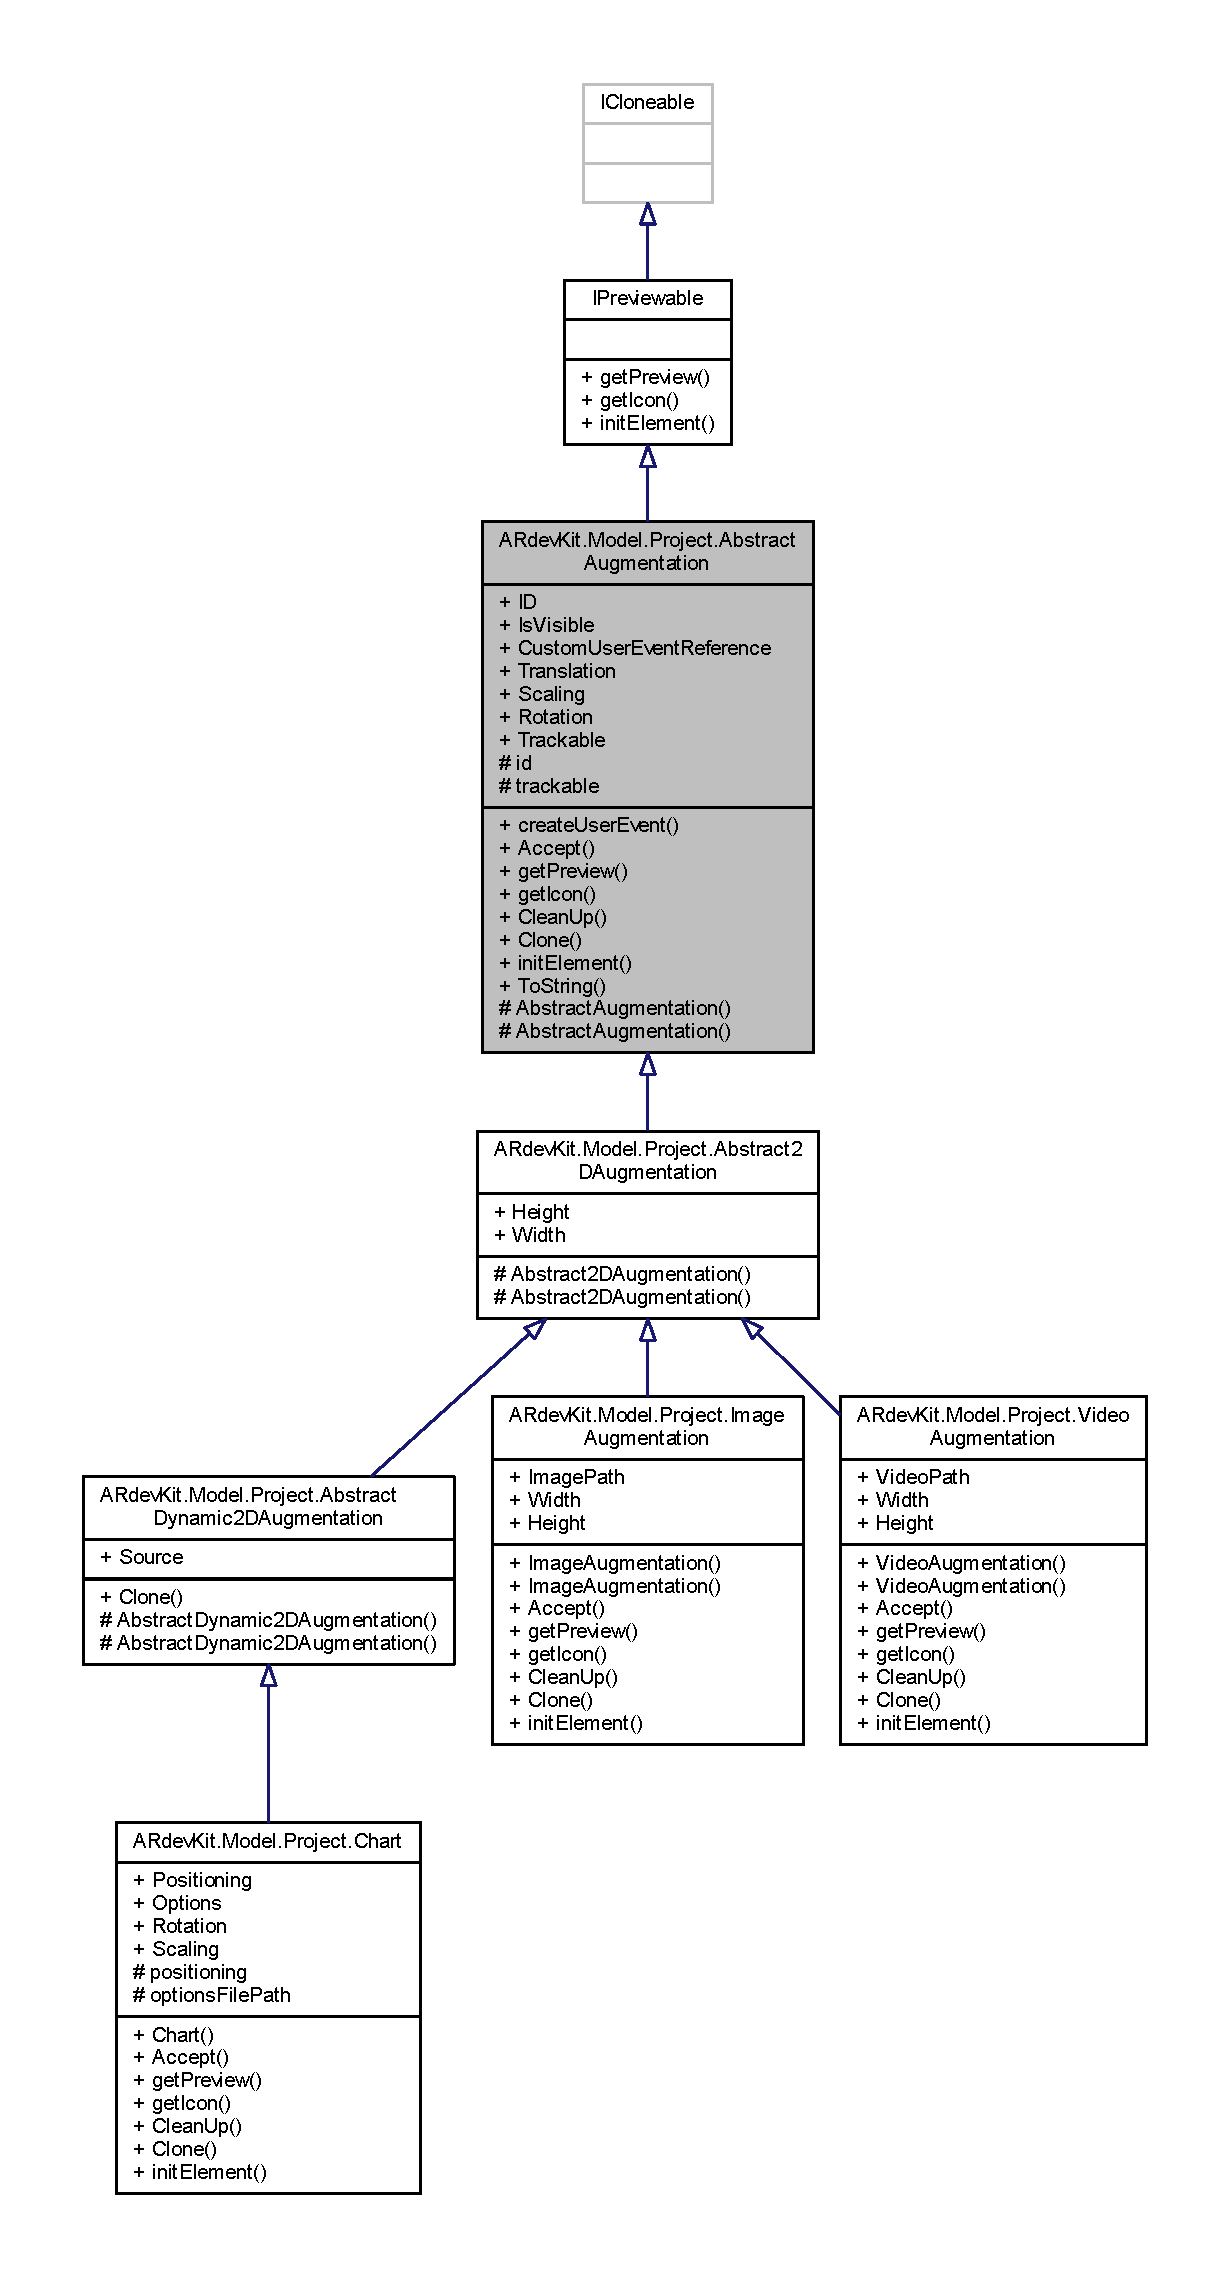
\includegraphics[height=550pt]{class_a_rdev_kit_1_1_model_1_1_project_1_1_abstract_augmentation__inherit__graph}
\end{center}
\end{figure}


Collaboration diagram for A\-Rdev\-Kit.\-Model.\-Project.\-Abstract\-Augmentation\-:
\nopagebreak
\begin{figure}[H]
\begin{center}
\leavevmode
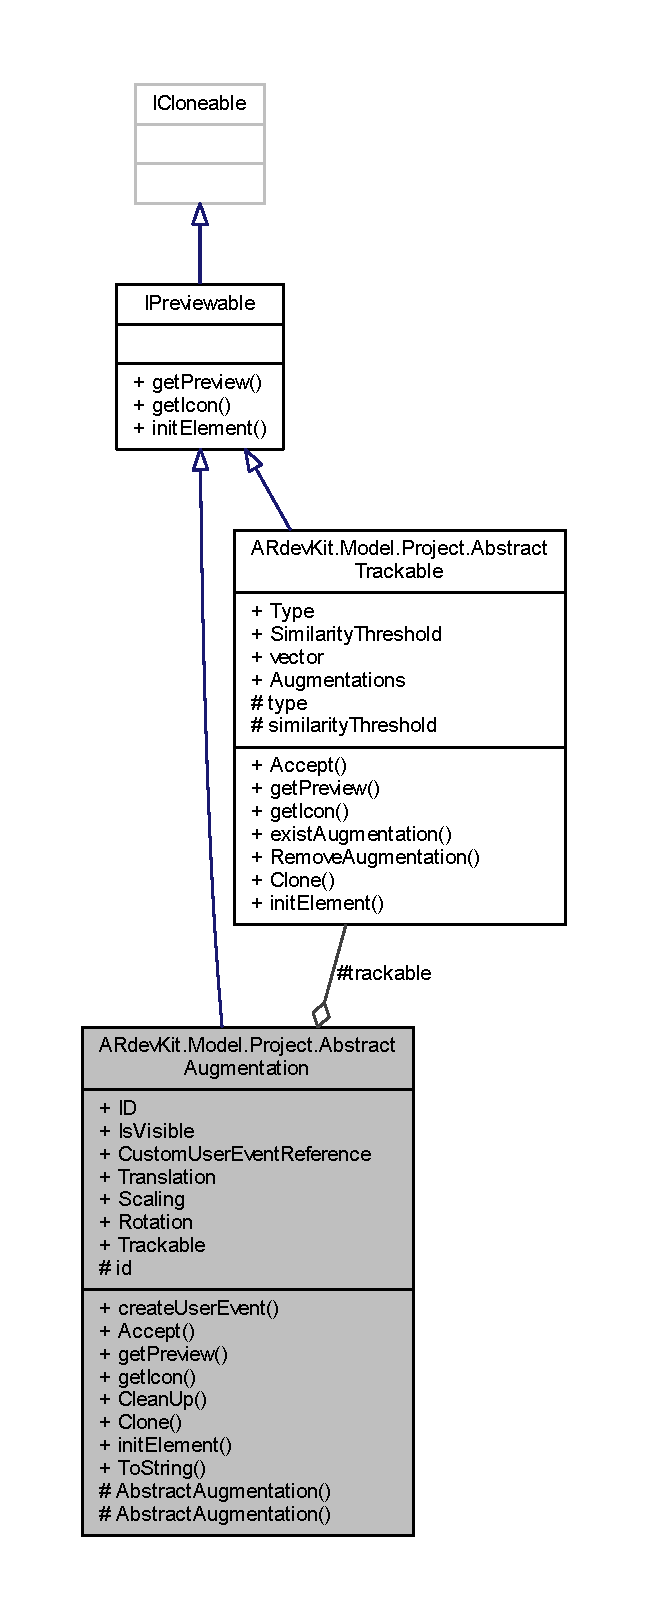
\includegraphics[height=550pt]{class_a_rdev_kit_1_1_model_1_1_project_1_1_abstract_augmentation__coll__graph}
\end{center}
\end{figure}
\subsection*{Public Member Functions}
\begin{DoxyCompactItemize}
\item 
void \hyperlink{class_a_rdev_kit_1_1_model_1_1_project_1_1_abstract_augmentation_a4f4497d02cdf208b57b4e3f90a6130fd}{create\-User\-Event} ()
\begin{DoxyCompactList}\small\item\em Method to create an instance of the \hyperlink{class_a_rdev_kit_1_1_model_1_1_project_1_1_custom_user_event}{Custom\-User\-Event}. \end{DoxyCompactList}\item 
virtual void \hyperlink{class_a_rdev_kit_1_1_model_1_1_project_1_1_abstract_augmentation_a2b3fa5e94428fab7f2d94842211a7cc9}{Accept} (\hyperlink{class_a_rdev_kit_1_1_controller_1_1_project_controller_1_1_abstract_project_visitor}{Abstract\-Project\-Visitor} visitor)
\begin{DoxyCompactList}\small\item\em An abstract method, to accept a Abstract\-Project\-Visitor which must be implemented according to the visitor design pattern. \end{DoxyCompactList}\item 
abstract Bitmap \hyperlink{class_a_rdev_kit_1_1_model_1_1_project_1_1_abstract_augmentation_a627330061b5df53ece5646e1cf83ff0f}{get\-Preview} ()
\begin{DoxyCompactList}\small\item\em returns a Bitmap in order to be displayed on the Preview\-Panel, implements \hyperlink{interface_a_rdev_kit_1_1_model_1_1_project_1_1_i_previewable}{I\-Previewable} \end{DoxyCompactList}\item 
abstract Bitmap \hyperlink{class_a_rdev_kit_1_1_model_1_1_project_1_1_abstract_augmentation_a703566211752c4c4e08ceb5b6c528918}{get\-Icon} ()
\begin{DoxyCompactList}\small\item\em returns a Bitmap in order to be displayed on the Element\-Selection\-Panel, implements \hyperlink{interface_a_rdev_kit_1_1_model_1_1_project_1_1_i_previewable}{I\-Previewable} \end{DoxyCompactList}\item 
abstract void \hyperlink{class_a_rdev_kit_1_1_model_1_1_project_1_1_abstract_augmentation_a29b5dcf0bea3da72b75707e09f42124f}{Clean\-Up} ()
\begin{DoxyCompactList}\small\item\em Clean up (remove created/copied files and directories). \end{DoxyCompactList}\item 
abstract object \hyperlink{class_a_rdev_kit_1_1_model_1_1_project_1_1_abstract_augmentation_a184416a3d47e35d58bb7f5bb6ce2e269}{Clone} ()
\begin{DoxyCompactList}\small\item\em Makes a deep copy of this object. \end{DoxyCompactList}\item 
virtual bool \hyperlink{class_a_rdev_kit_1_1_model_1_1_project_1_1_abstract_augmentation_a8b02a2eb775b8147e71575694ce8a38f}{init\-Element} (\hyperlink{class_a_rdev_kit_1_1_editor_window}{Editor\-Window} ew)
\begin{DoxyCompactList}\small\item\em This method is called by the preview\-Controller when a new instance of the element is added to the Scene. It sets \char`\"{}must-\/have\char`\"{} properties. \end{DoxyCompactList}\item 
override string \hyperlink{class_a_rdev_kit_1_1_model_1_1_project_1_1_abstract_augmentation_aa3badea1be1d6317e62e2dda390c2f34}{To\-String} ()
\begin{DoxyCompactList}\small\item\em Gibt eine Zeichenfolge zurück, die das aktuelle Objekt darstellt. \end{DoxyCompactList}\end{DoxyCompactItemize}
\subsection*{Protected Member Functions}
\begin{DoxyCompactItemize}
\item 
\hyperlink{class_a_rdev_kit_1_1_model_1_1_project_1_1_abstract_augmentation_a6dcd315fd15d4dd67a6910624cb38fb8}{Abstract\-Augmentation} ()
\begin{DoxyCompactList}\small\item\em Initializes no new instance of the \hyperlink{class_a_rdev_kit_1_1_model_1_1_project_1_1_abstract_augmentation}{Abstract\-Augmentation} class, but can be used in inheriting classes. Using standard values, such as empty\-Lists, vectors with 0 as coordinate and null. \end{DoxyCompactList}\item 
\hyperlink{class_a_rdev_kit_1_1_model_1_1_project_1_1_abstract_augmentation_a46d8ded608fcaf37e6597e789c052e52}{Abstract\-Augmentation} (bool is\-Visible, \hyperlink{class_a_rdev_kit_1_1_model_1_1_project_1_1_vector3_d}{Vector3\-D} translation\-Vector, \hyperlink{class_a_rdev_kit_1_1_model_1_1_project_1_1_vector3_d}{Vector3\-D} scaling, \hyperlink{class_a_rdev_kit_1_1_model_1_1_project_1_1_abstract_trackable}{Abstract\-Trackable} \hyperlink{class_a_rdev_kit_1_1_model_1_1_project_1_1_abstract_augmentation_a8d8e3f3c42696008edbfc44d51ba518d}{trackable})
\begin{DoxyCompactList}\small\item\em Initializes no new instance of the \hyperlink{class_a_rdev_kit_1_1_model_1_1_project_1_1_abstract_augmentation}{Abstract\-Augmentation} class, but can be used in inheriting classes. \end{DoxyCompactList}\end{DoxyCompactItemize}
\subsection*{Protected Attributes}
\begin{DoxyCompactItemize}
\item 
string \hyperlink{class_a_rdev_kit_1_1_model_1_1_project_1_1_abstract_augmentation_af0470569d324d3bf199a841be3a3e853}{id}
\begin{DoxyCompactList}\small\item\em The identifier. \end{DoxyCompactList}\item 
\hyperlink{class_a_rdev_kit_1_1_model_1_1_project_1_1_abstract_trackable}{Abstract\-Trackable} \hyperlink{class_a_rdev_kit_1_1_model_1_1_project_1_1_abstract_augmentation_a8d8e3f3c42696008edbfc44d51ba518d}{trackable}
\begin{DoxyCompactList}\small\item\em The \hyperlink{class_a_rdev_kit_1_1_model_1_1_project_1_1_abstract_trackable}{Abstract\-Trackable} with which this \hyperlink{class_a_rdev_kit_1_1_model_1_1_project_1_1_abstract_augmentation}{Abstract\-Augmentation} is linked. It is visible in the same Scene as the trackable. \end{DoxyCompactList}\end{DoxyCompactItemize}
\subsection*{Properties}
\begin{DoxyCompactItemize}
\item 
string \hyperlink{class_a_rdev_kit_1_1_model_1_1_project_1_1_abstract_augmentation_a3590cc30e6169c0946c70b52223eb2bf}{I\-D}\hspace{0.3cm}{\ttfamily  \mbox{[}get, set\mbox{]}}
\begin{DoxyCompactList}\small\item\em Gets or sets the identifier. \end{DoxyCompactList}\item 
bool \hyperlink{class_a_rdev_kit_1_1_model_1_1_project_1_1_abstract_augmentation_ab19dda553062c0cae9e4a7a66e9cb64f}{Is\-Visible}\hspace{0.3cm}{\ttfamily  \mbox{[}get, set\mbox{]}}
\begin{DoxyCompactList}\small\item\em Get or set if the \hyperlink{class_a_rdev_kit_1_1_model_1_1_project_1_1_abstract_augmentation}{Abstract\-Augmentation} is visible the whole time using A\-R\-E\-L or not. \end{DoxyCompactList}\item 
\hyperlink{class_a_rdev_kit_1_1_model_1_1_project_1_1_custom_user_event}{Custom\-User\-Event} \hyperlink{class_a_rdev_kit_1_1_model_1_1_project_1_1_abstract_augmentation_a333186e3963596bc5b17c02a21f2d384}{Custom\-User\-Event\-Reference}\hspace{0.3cm}{\ttfamily  \mbox{[}get, set\mbox{]}}
\begin{DoxyCompactList}\small\item\em Get the \hyperlink{class_a_rdev_kit_1_1_model_1_1_project_1_1_custom_user_event}{Custom\-User\-Event}. \end{DoxyCompactList}\item 
\hyperlink{class_a_rdev_kit_1_1_model_1_1_project_1_1_vector3_d}{Vector3\-D} \hyperlink{class_a_rdev_kit_1_1_model_1_1_project_1_1_abstract_augmentation_a8ed7943a2eb75682addda8731bff6c34}{Translation}\hspace{0.3cm}{\ttfamily  \mbox{[}get, set\mbox{]}}
\begin{DoxyCompactList}\small\item\em Get or set the position of the \hyperlink{class_a_rdev_kit_1_1_model_1_1_project_1_1_abstract_augmentation}{Abstract\-Augmentation}. \end{DoxyCompactList}\item 
\hyperlink{class_a_rdev_kit_1_1_model_1_1_project_1_1_vector3_d}{Vector3\-D} \hyperlink{class_a_rdev_kit_1_1_model_1_1_project_1_1_abstract_augmentation_adc3b84e8eb93f1ef50b3a689bd4c2a72}{Scaling}\hspace{0.3cm}{\ttfamily  \mbox{[}get, set\mbox{]}}
\begin{DoxyCompactList}\small\item\em gets or sets the scaling which is applied to the original \hyperlink{class_a_rdev_kit_1_1_model_1_1_project_1_1_abstract_augmentation}{Abstract\-Augmentation} \end{DoxyCompactList}\item 
\hyperlink{class_a_rdev_kit_1_1_model_1_1_project_1_1_vector3_d}{Vector3\-D} \hyperlink{class_a_rdev_kit_1_1_model_1_1_project_1_1_abstract_augmentation_ac94095d5fa4f5d4339f66b259ff55e74}{Rotation}\hspace{0.3cm}{\ttfamily  \mbox{[}get, set\mbox{]}}
\begin{DoxyCompactList}\small\item\em gets or sets the Vector \end{DoxyCompactList}\item 
\hyperlink{class_a_rdev_kit_1_1_model_1_1_project_1_1_abstract_trackable}{Abstract\-Trackable} \hyperlink{class_a_rdev_kit_1_1_model_1_1_project_1_1_abstract_augmentation_a5ef95a16a1d2b03cb6185b86e7120a9c}{Trackable}\hspace{0.3cm}{\ttfamily  \mbox{[}get, set\mbox{]}}
\begin{DoxyCompactList}\small\item\em Get or set a trackable to the augmentation. \end{DoxyCompactList}\end{DoxyCompactItemize}


\subsection{Detailed Description}
describes an \hyperlink{class_a_rdev_kit_1_1_model_1_1_project_1_1_abstract_augmentation}{Abstract\-Augmentation}, which is bound to a certain \hyperlink{class_a_rdev_kit_1_1_model_1_1_project_1_1_abstract_trackable}{Abstract\-Trackable}. is \hyperlink{interface_a_rdev_kit_1_1_model_1_1_project_1_1_i_previewable}{I\-Previewable} 



\subsection{Constructor \& Destructor Documentation}
\hypertarget{class_a_rdev_kit_1_1_model_1_1_project_1_1_abstract_augmentation_a6dcd315fd15d4dd67a6910624cb38fb8}{\index{A\-Rdev\-Kit\-::\-Model\-::\-Project\-::\-Abstract\-Augmentation@{A\-Rdev\-Kit\-::\-Model\-::\-Project\-::\-Abstract\-Augmentation}!Abstract\-Augmentation@{Abstract\-Augmentation}}
\index{Abstract\-Augmentation@{Abstract\-Augmentation}!ARdevKit::Model::Project::AbstractAugmentation@{A\-Rdev\-Kit\-::\-Model\-::\-Project\-::\-Abstract\-Augmentation}}
\subsubsection[{Abstract\-Augmentation}]{\setlength{\rightskip}{0pt plus 5cm}A\-Rdev\-Kit.\-Model.\-Project.\-Abstract\-Augmentation.\-Abstract\-Augmentation (
\begin{DoxyParamCaption}
{}
\end{DoxyParamCaption}
)\hspace{0.3cm}{\ttfamily [protected]}}}\label{class_a_rdev_kit_1_1_model_1_1_project_1_1_abstract_augmentation_a6dcd315fd15d4dd67a6910624cb38fb8}


Initializes no new instance of the \hyperlink{class_a_rdev_kit_1_1_model_1_1_project_1_1_abstract_augmentation}{Abstract\-Augmentation} class, but can be used in inheriting classes. Using standard values, such as empty\-Lists, vectors with 0 as coordinate and null. 

\hypertarget{class_a_rdev_kit_1_1_model_1_1_project_1_1_abstract_augmentation_a46d8ded608fcaf37e6597e789c052e52}{\index{A\-Rdev\-Kit\-::\-Model\-::\-Project\-::\-Abstract\-Augmentation@{A\-Rdev\-Kit\-::\-Model\-::\-Project\-::\-Abstract\-Augmentation}!Abstract\-Augmentation@{Abstract\-Augmentation}}
\index{Abstract\-Augmentation@{Abstract\-Augmentation}!ARdevKit::Model::Project::AbstractAugmentation@{A\-Rdev\-Kit\-::\-Model\-::\-Project\-::\-Abstract\-Augmentation}}
\subsubsection[{Abstract\-Augmentation}]{\setlength{\rightskip}{0pt plus 5cm}A\-Rdev\-Kit.\-Model.\-Project.\-Abstract\-Augmentation.\-Abstract\-Augmentation (
\begin{DoxyParamCaption}
\item[{bool}]{is\-Visible, }
\item[{{\bf Vector3\-D}}]{translation\-Vector, }
\item[{{\bf Vector3\-D}}]{scaling, }
\item[{{\bf Abstract\-Trackable}}]{trackable}
\end{DoxyParamCaption}
)\hspace{0.3cm}{\ttfamily [protected]}}}\label{class_a_rdev_kit_1_1_model_1_1_project_1_1_abstract_augmentation_a46d8ded608fcaf37e6597e789c052e52}


Initializes no new instance of the \hyperlink{class_a_rdev_kit_1_1_model_1_1_project_1_1_abstract_augmentation}{Abstract\-Augmentation} class, but can be used in inheriting classes. 


\begin{DoxyParams}{Parameters}
{\em is\-Visible} & if set to {\ttfamily true} \mbox{[}is visible\mbox{]} using A\-R\-E\-L.\\
\hline
{\em translation\-Vector} & The translation vector.\\
\hline
{\em scaling} & The scaling.\\
\hline
{\em trackable} & The trackable.\\
\hline
\end{DoxyParams}


\subsection{Member Function Documentation}
\hypertarget{class_a_rdev_kit_1_1_model_1_1_project_1_1_abstract_augmentation_a2b3fa5e94428fab7f2d94842211a7cc9}{\index{A\-Rdev\-Kit\-::\-Model\-::\-Project\-::\-Abstract\-Augmentation@{A\-Rdev\-Kit\-::\-Model\-::\-Project\-::\-Abstract\-Augmentation}!Accept@{Accept}}
\index{Accept@{Accept}!ARdevKit::Model::Project::AbstractAugmentation@{A\-Rdev\-Kit\-::\-Model\-::\-Project\-::\-Abstract\-Augmentation}}
\subsubsection[{Accept}]{\setlength{\rightskip}{0pt plus 5cm}virtual void A\-Rdev\-Kit.\-Model.\-Project.\-Abstract\-Augmentation.\-Accept (
\begin{DoxyParamCaption}
\item[{{\bf Abstract\-Project\-Visitor}}]{visitor}
\end{DoxyParamCaption}
)\hspace{0.3cm}{\ttfamily [virtual]}}}\label{class_a_rdev_kit_1_1_model_1_1_project_1_1_abstract_augmentation_a2b3fa5e94428fab7f2d94842211a7cc9}


An abstract method, to accept a Abstract\-Project\-Visitor which must be implemented according to the visitor design pattern. 


\begin{DoxyParams}{Parameters}
{\em visitor} & the visitor which encapsulates the action which is performed on this element\\
\hline
\end{DoxyParams}


Reimplemented in \hyperlink{class_a_rdev_kit_1_1_model_1_1_project_1_1_image_augmentation_a1450cf89881f65c8882126914379ae50}{A\-Rdev\-Kit.\-Model.\-Project.\-Image\-Augmentation}, and \hyperlink{class_a_rdev_kit_1_1_model_1_1_project_1_1_video_augmentation_a7f23dea6de8cd95e5500e5000245d118}{A\-Rdev\-Kit.\-Model.\-Project.\-Video\-Augmentation}.

\hypertarget{class_a_rdev_kit_1_1_model_1_1_project_1_1_abstract_augmentation_a29b5dcf0bea3da72b75707e09f42124f}{\index{A\-Rdev\-Kit\-::\-Model\-::\-Project\-::\-Abstract\-Augmentation@{A\-Rdev\-Kit\-::\-Model\-::\-Project\-::\-Abstract\-Augmentation}!Clean\-Up@{Clean\-Up}}
\index{Clean\-Up@{Clean\-Up}!ARdevKit::Model::Project::AbstractAugmentation@{A\-Rdev\-Kit\-::\-Model\-::\-Project\-::\-Abstract\-Augmentation}}
\subsubsection[{Clean\-Up}]{\setlength{\rightskip}{0pt plus 5cm}abstract void A\-Rdev\-Kit.\-Model.\-Project.\-Abstract\-Augmentation.\-Clean\-Up (
\begin{DoxyParamCaption}
{}
\end{DoxyParamCaption}
)\hspace{0.3cm}{\ttfamily [pure virtual]}}}\label{class_a_rdev_kit_1_1_model_1_1_project_1_1_abstract_augmentation_a29b5dcf0bea3da72b75707e09f42124f}


Clean up (remove created/copied files and directories). 

Imanuel, 31.\-01.\-2014. 

Implemented in \hyperlink{class_a_rdev_kit_1_1_model_1_1_project_1_1_chart_a5cccd28644f1f358d551028759a3fed0}{A\-Rdev\-Kit.\-Model.\-Project.\-Chart}, \hyperlink{class_a_rdev_kit_1_1_model_1_1_project_1_1_video_augmentation_a83390b8765641d1626b23a06c54490af}{A\-Rdev\-Kit.\-Model.\-Project.\-Video\-Augmentation}, and \hyperlink{class_a_rdev_kit_1_1_model_1_1_project_1_1_image_augmentation_aecb9401ae2f65c089330e280af41d55a}{A\-Rdev\-Kit.\-Model.\-Project.\-Image\-Augmentation}.

\hypertarget{class_a_rdev_kit_1_1_model_1_1_project_1_1_abstract_augmentation_a184416a3d47e35d58bb7f5bb6ce2e269}{\index{A\-Rdev\-Kit\-::\-Model\-::\-Project\-::\-Abstract\-Augmentation@{A\-Rdev\-Kit\-::\-Model\-::\-Project\-::\-Abstract\-Augmentation}!Clone@{Clone}}
\index{Clone@{Clone}!ARdevKit::Model::Project::AbstractAugmentation@{A\-Rdev\-Kit\-::\-Model\-::\-Project\-::\-Abstract\-Augmentation}}
\subsubsection[{Clone}]{\setlength{\rightskip}{0pt plus 5cm}abstract object A\-Rdev\-Kit.\-Model.\-Project.\-Abstract\-Augmentation.\-Clone (
\begin{DoxyParamCaption}
{}
\end{DoxyParamCaption}
)\hspace{0.3cm}{\ttfamily [pure virtual]}}}\label{class_a_rdev_kit_1_1_model_1_1_project_1_1_abstract_augmentation_a184416a3d47e35d58bb7f5bb6ce2e269}


Makes a deep copy of this object. 

Robin, 22.\-01.\-2014. 

\begin{DoxyReturn}{Returns}
A copy of this object. 
\end{DoxyReturn}


Implemented in \hyperlink{class_a_rdev_kit_1_1_model_1_1_project_1_1_chart_aaa06b6e53f2e5a48508f3a93b0483dc3}{A\-Rdev\-Kit.\-Model.\-Project.\-Chart}, \hyperlink{class_a_rdev_kit_1_1_model_1_1_project_1_1_video_augmentation_a1c99b0002e89662c75ae59031f1f7ec5}{A\-Rdev\-Kit.\-Model.\-Project.\-Video\-Augmentation}, \hyperlink{class_a_rdev_kit_1_1_model_1_1_project_1_1_image_augmentation_af25172abfef48a1f9004ec3777d0d6fb}{A\-Rdev\-Kit.\-Model.\-Project.\-Image\-Augmentation}, and \hyperlink{class_a_rdev_kit_1_1_model_1_1_project_1_1_abstract_dynamic2_d_augmentation_adbb2d06450362f0385fe937bbb5255a8}{A\-Rdev\-Kit.\-Model.\-Project.\-Abstract\-Dynamic2\-D\-Augmentation}.



Here is the caller graph for this function\-:
\nopagebreak
\begin{figure}[H]
\begin{center}
\leavevmode
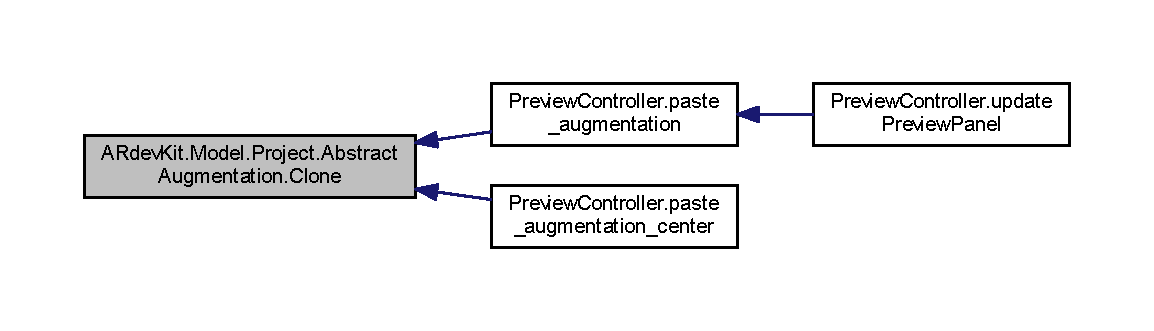
\includegraphics[width=350pt]{class_a_rdev_kit_1_1_model_1_1_project_1_1_abstract_augmentation_a184416a3d47e35d58bb7f5bb6ce2e269_icgraph}
\end{center}
\end{figure}


\hypertarget{class_a_rdev_kit_1_1_model_1_1_project_1_1_abstract_augmentation_a4f4497d02cdf208b57b4e3f90a6130fd}{\index{A\-Rdev\-Kit\-::\-Model\-::\-Project\-::\-Abstract\-Augmentation@{A\-Rdev\-Kit\-::\-Model\-::\-Project\-::\-Abstract\-Augmentation}!create\-User\-Event@{create\-User\-Event}}
\index{create\-User\-Event@{create\-User\-Event}!ARdevKit::Model::Project::AbstractAugmentation@{A\-Rdev\-Kit\-::\-Model\-::\-Project\-::\-Abstract\-Augmentation}}
\subsubsection[{create\-User\-Event}]{\setlength{\rightskip}{0pt plus 5cm}void A\-Rdev\-Kit.\-Model.\-Project.\-Abstract\-Augmentation.\-create\-User\-Event (
\begin{DoxyParamCaption}
{}
\end{DoxyParamCaption}
)}}\label{class_a_rdev_kit_1_1_model_1_1_project_1_1_abstract_augmentation_a4f4497d02cdf208b57b4e3f90a6130fd}


Method to create an instance of the \hyperlink{class_a_rdev_kit_1_1_model_1_1_project_1_1_custom_user_event}{Custom\-User\-Event}. 

\hypertarget{class_a_rdev_kit_1_1_model_1_1_project_1_1_abstract_augmentation_a703566211752c4c4e08ceb5b6c528918}{\index{A\-Rdev\-Kit\-::\-Model\-::\-Project\-::\-Abstract\-Augmentation@{A\-Rdev\-Kit\-::\-Model\-::\-Project\-::\-Abstract\-Augmentation}!get\-Icon@{get\-Icon}}
\index{get\-Icon@{get\-Icon}!ARdevKit::Model::Project::AbstractAugmentation@{A\-Rdev\-Kit\-::\-Model\-::\-Project\-::\-Abstract\-Augmentation}}
\subsubsection[{get\-Icon}]{\setlength{\rightskip}{0pt plus 5cm}abstract Bitmap A\-Rdev\-Kit.\-Model.\-Project.\-Abstract\-Augmentation.\-get\-Icon (
\begin{DoxyParamCaption}
{}
\end{DoxyParamCaption}
)\hspace{0.3cm}{\ttfamily [pure virtual]}}}\label{class_a_rdev_kit_1_1_model_1_1_project_1_1_abstract_augmentation_a703566211752c4c4e08ceb5b6c528918}


returns a Bitmap in order to be displayed on the Element\-Selection\-Panel, implements \hyperlink{interface_a_rdev_kit_1_1_model_1_1_project_1_1_i_previewable}{I\-Previewable} 

\begin{DoxyReturn}{Returns}
a representative iconized Bitmap
\end{DoxyReturn}


Implements \hyperlink{interface_a_rdev_kit_1_1_model_1_1_project_1_1_i_previewable_a8573bdaccd5227400b538c34c1b5f279}{A\-Rdev\-Kit.\-Model.\-Project.\-I\-Previewable}.



Implemented in \hyperlink{class_a_rdev_kit_1_1_model_1_1_project_1_1_chart_a5a3555ace98e2f5c9f4daaa73f94cd96}{A\-Rdev\-Kit.\-Model.\-Project.\-Chart}, \hyperlink{class_a_rdev_kit_1_1_model_1_1_project_1_1_video_augmentation_ae41611da8c40607d32ab62d29c78a8ae}{A\-Rdev\-Kit.\-Model.\-Project.\-Video\-Augmentation}, and \hyperlink{class_a_rdev_kit_1_1_model_1_1_project_1_1_image_augmentation_a7f1d0335a2559d461cbe18599ce472c2}{A\-Rdev\-Kit.\-Model.\-Project.\-Image\-Augmentation}.

\hypertarget{class_a_rdev_kit_1_1_model_1_1_project_1_1_abstract_augmentation_a627330061b5df53ece5646e1cf83ff0f}{\index{A\-Rdev\-Kit\-::\-Model\-::\-Project\-::\-Abstract\-Augmentation@{A\-Rdev\-Kit\-::\-Model\-::\-Project\-::\-Abstract\-Augmentation}!get\-Preview@{get\-Preview}}
\index{get\-Preview@{get\-Preview}!ARdevKit::Model::Project::AbstractAugmentation@{A\-Rdev\-Kit\-::\-Model\-::\-Project\-::\-Abstract\-Augmentation}}
\subsubsection[{get\-Preview}]{\setlength{\rightskip}{0pt plus 5cm}abstract Bitmap A\-Rdev\-Kit.\-Model.\-Project.\-Abstract\-Augmentation.\-get\-Preview (
\begin{DoxyParamCaption}
{}
\end{DoxyParamCaption}
)\hspace{0.3cm}{\ttfamily [pure virtual]}}}\label{class_a_rdev_kit_1_1_model_1_1_project_1_1_abstract_augmentation_a627330061b5df53ece5646e1cf83ff0f}


returns a Bitmap in order to be displayed on the Preview\-Panel, implements \hyperlink{interface_a_rdev_kit_1_1_model_1_1_project_1_1_i_previewable}{I\-Previewable} 

\begin{DoxyReturn}{Returns}
a representative Bitmap
\end{DoxyReturn}


Implements \hyperlink{interface_a_rdev_kit_1_1_model_1_1_project_1_1_i_previewable_a7cbcbb20929f4f1b6db3321ed2e83070}{A\-Rdev\-Kit.\-Model.\-Project.\-I\-Previewable}.



Implemented in \hyperlink{class_a_rdev_kit_1_1_model_1_1_project_1_1_chart_aab1b49aedaba3798818abd14c69918e8}{A\-Rdev\-Kit.\-Model.\-Project.\-Chart}, \hyperlink{class_a_rdev_kit_1_1_model_1_1_project_1_1_image_augmentation_a76230c0eb40c317bab23b37c27ea3a39}{A\-Rdev\-Kit.\-Model.\-Project.\-Image\-Augmentation}, and \hyperlink{class_a_rdev_kit_1_1_model_1_1_project_1_1_video_augmentation_a3d5968ace1fe7b6becfc10b60f573631}{A\-Rdev\-Kit.\-Model.\-Project.\-Video\-Augmentation}.

\hypertarget{class_a_rdev_kit_1_1_model_1_1_project_1_1_abstract_augmentation_a8b02a2eb775b8147e71575694ce8a38f}{\index{A\-Rdev\-Kit\-::\-Model\-::\-Project\-::\-Abstract\-Augmentation@{A\-Rdev\-Kit\-::\-Model\-::\-Project\-::\-Abstract\-Augmentation}!init\-Element@{init\-Element}}
\index{init\-Element@{init\-Element}!ARdevKit::Model::Project::AbstractAugmentation@{A\-Rdev\-Kit\-::\-Model\-::\-Project\-::\-Abstract\-Augmentation}}
\subsubsection[{init\-Element}]{\setlength{\rightskip}{0pt plus 5cm}virtual bool A\-Rdev\-Kit.\-Model.\-Project.\-Abstract\-Augmentation.\-init\-Element (
\begin{DoxyParamCaption}
\item[{{\bf Editor\-Window}}]{ew}
\end{DoxyParamCaption}
)\hspace{0.3cm}{\ttfamily [virtual]}}}\label{class_a_rdev_kit_1_1_model_1_1_project_1_1_abstract_augmentation_a8b02a2eb775b8147e71575694ce8a38f}


This method is called by the preview\-Controller when a new instance of the element is added to the Scene. It sets \char`\"{}must-\/have\char`\"{} properties. 


\begin{DoxyParams}{Parameters}
{\em ew} & The ew.\\
\hline
\end{DoxyParams}
\begin{DoxyReturn}{Returns}
true if it succeeds, false if it fails. 
\end{DoxyReturn}


Implements \hyperlink{interface_a_rdev_kit_1_1_model_1_1_project_1_1_i_previewable_aa638e27d88c30b7e63b241d1001042c9}{A\-Rdev\-Kit.\-Model.\-Project.\-I\-Previewable}.



Reimplemented in \hyperlink{class_a_rdev_kit_1_1_model_1_1_project_1_1_chart_a74620f6abc6763b5999074c5c6e2f661}{A\-Rdev\-Kit.\-Model.\-Project.\-Chart}, \hyperlink{class_a_rdev_kit_1_1_model_1_1_project_1_1_video_augmentation_afb33f9a8ac2591973d29ebd56bd75da5}{A\-Rdev\-Kit.\-Model.\-Project.\-Video\-Augmentation}, and \hyperlink{class_a_rdev_kit_1_1_model_1_1_project_1_1_image_augmentation_a37ba80403f194a8aad7e7b96a8fd9239}{A\-Rdev\-Kit.\-Model.\-Project.\-Image\-Augmentation}.

\hypertarget{class_a_rdev_kit_1_1_model_1_1_project_1_1_abstract_augmentation_aa3badea1be1d6317e62e2dda390c2f34}{\index{A\-Rdev\-Kit\-::\-Model\-::\-Project\-::\-Abstract\-Augmentation@{A\-Rdev\-Kit\-::\-Model\-::\-Project\-::\-Abstract\-Augmentation}!To\-String@{To\-String}}
\index{To\-String@{To\-String}!ARdevKit::Model::Project::AbstractAugmentation@{A\-Rdev\-Kit\-::\-Model\-::\-Project\-::\-Abstract\-Augmentation}}
\subsubsection[{To\-String}]{\setlength{\rightskip}{0pt plus 5cm}override string A\-Rdev\-Kit.\-Model.\-Project.\-Abstract\-Augmentation.\-To\-String (
\begin{DoxyParamCaption}
{}
\end{DoxyParamCaption}
)}}\label{class_a_rdev_kit_1_1_model_1_1_project_1_1_abstract_augmentation_aa3badea1be1d6317e62e2dda390c2f34}


Gibt eine Zeichenfolge zurück, die das aktuelle Objekt darstellt. 

Robin, 14.\-01.\-2014. 

\begin{DoxyReturn}{Returns}
Eine Zeichenfolge, die das aktuelle Objekt darstellt. 
\end{DoxyReturn}


\subsection{Member Data Documentation}
\hypertarget{class_a_rdev_kit_1_1_model_1_1_project_1_1_abstract_augmentation_af0470569d324d3bf199a841be3a3e853}{\index{A\-Rdev\-Kit\-::\-Model\-::\-Project\-::\-Abstract\-Augmentation@{A\-Rdev\-Kit\-::\-Model\-::\-Project\-::\-Abstract\-Augmentation}!id@{id}}
\index{id@{id}!ARdevKit::Model::Project::AbstractAugmentation@{A\-Rdev\-Kit\-::\-Model\-::\-Project\-::\-Abstract\-Augmentation}}
\subsubsection[{id}]{\setlength{\rightskip}{0pt plus 5cm}string A\-Rdev\-Kit.\-Model.\-Project.\-Abstract\-Augmentation.\-id\hspace{0.3cm}{\ttfamily [protected]}}}\label{class_a_rdev_kit_1_1_model_1_1_project_1_1_abstract_augmentation_af0470569d324d3bf199a841be3a3e853}


The identifier. 

\hypertarget{class_a_rdev_kit_1_1_model_1_1_project_1_1_abstract_augmentation_a8d8e3f3c42696008edbfc44d51ba518d}{\index{A\-Rdev\-Kit\-::\-Model\-::\-Project\-::\-Abstract\-Augmentation@{A\-Rdev\-Kit\-::\-Model\-::\-Project\-::\-Abstract\-Augmentation}!trackable@{trackable}}
\index{trackable@{trackable}!ARdevKit::Model::Project::AbstractAugmentation@{A\-Rdev\-Kit\-::\-Model\-::\-Project\-::\-Abstract\-Augmentation}}
\subsubsection[{trackable}]{\setlength{\rightskip}{0pt plus 5cm}{\bf Abstract\-Trackable} A\-Rdev\-Kit.\-Model.\-Project.\-Abstract\-Augmentation.\-trackable\hspace{0.3cm}{\ttfamily [protected]}}}\label{class_a_rdev_kit_1_1_model_1_1_project_1_1_abstract_augmentation_a8d8e3f3c42696008edbfc44d51ba518d}


The \hyperlink{class_a_rdev_kit_1_1_model_1_1_project_1_1_abstract_trackable}{Abstract\-Trackable} with which this \hyperlink{class_a_rdev_kit_1_1_model_1_1_project_1_1_abstract_augmentation}{Abstract\-Augmentation} is linked. It is visible in the same Scene as the trackable. 



\subsection{Property Documentation}
\hypertarget{class_a_rdev_kit_1_1_model_1_1_project_1_1_abstract_augmentation_a333186e3963596bc5b17c02a21f2d384}{\index{A\-Rdev\-Kit\-::\-Model\-::\-Project\-::\-Abstract\-Augmentation@{A\-Rdev\-Kit\-::\-Model\-::\-Project\-::\-Abstract\-Augmentation}!Custom\-User\-Event\-Reference@{Custom\-User\-Event\-Reference}}
\index{Custom\-User\-Event\-Reference@{Custom\-User\-Event\-Reference}!ARdevKit::Model::Project::AbstractAugmentation@{A\-Rdev\-Kit\-::\-Model\-::\-Project\-::\-Abstract\-Augmentation}}
\subsubsection[{Custom\-User\-Event\-Reference}]{\setlength{\rightskip}{0pt plus 5cm}{\bf Custom\-User\-Event} A\-Rdev\-Kit.\-Model.\-Project.\-Abstract\-Augmentation.\-Custom\-User\-Event\-Reference\hspace{0.3cm}{\ttfamily [get]}, {\ttfamily [set]}}}\label{class_a_rdev_kit_1_1_model_1_1_project_1_1_abstract_augmentation_a333186e3963596bc5b17c02a21f2d384}


Get the \hyperlink{class_a_rdev_kit_1_1_model_1_1_project_1_1_custom_user_event}{Custom\-User\-Event}. 

\hypertarget{class_a_rdev_kit_1_1_model_1_1_project_1_1_abstract_augmentation_a3590cc30e6169c0946c70b52223eb2bf}{\index{A\-Rdev\-Kit\-::\-Model\-::\-Project\-::\-Abstract\-Augmentation@{A\-Rdev\-Kit\-::\-Model\-::\-Project\-::\-Abstract\-Augmentation}!I\-D@{I\-D}}
\index{I\-D@{I\-D}!ARdevKit::Model::Project::AbstractAugmentation@{A\-Rdev\-Kit\-::\-Model\-::\-Project\-::\-Abstract\-Augmentation}}
\subsubsection[{I\-D}]{\setlength{\rightskip}{0pt plus 5cm}string A\-Rdev\-Kit.\-Model.\-Project.\-Abstract\-Augmentation.\-I\-D\hspace{0.3cm}{\ttfamily [get]}, {\ttfamily [set]}}}\label{class_a_rdev_kit_1_1_model_1_1_project_1_1_abstract_augmentation_a3590cc30e6169c0946c70b52223eb2bf}


Gets or sets the identifier. 

The identifier. \hypertarget{class_a_rdev_kit_1_1_model_1_1_project_1_1_abstract_augmentation_ab19dda553062c0cae9e4a7a66e9cb64f}{\index{A\-Rdev\-Kit\-::\-Model\-::\-Project\-::\-Abstract\-Augmentation@{A\-Rdev\-Kit\-::\-Model\-::\-Project\-::\-Abstract\-Augmentation}!Is\-Visible@{Is\-Visible}}
\index{Is\-Visible@{Is\-Visible}!ARdevKit::Model::Project::AbstractAugmentation@{A\-Rdev\-Kit\-::\-Model\-::\-Project\-::\-Abstract\-Augmentation}}
\subsubsection[{Is\-Visible}]{\setlength{\rightskip}{0pt plus 5cm}bool A\-Rdev\-Kit.\-Model.\-Project.\-Abstract\-Augmentation.\-Is\-Visible\hspace{0.3cm}{\ttfamily [get]}, {\ttfamily [set]}}}\label{class_a_rdev_kit_1_1_model_1_1_project_1_1_abstract_augmentation_ab19dda553062c0cae9e4a7a66e9cb64f}


Get or set if the \hyperlink{class_a_rdev_kit_1_1_model_1_1_project_1_1_abstract_augmentation}{Abstract\-Augmentation} is visible the whole time using A\-R\-E\-L or not. 

\hypertarget{class_a_rdev_kit_1_1_model_1_1_project_1_1_abstract_augmentation_ac94095d5fa4f5d4339f66b259ff55e74}{\index{A\-Rdev\-Kit\-::\-Model\-::\-Project\-::\-Abstract\-Augmentation@{A\-Rdev\-Kit\-::\-Model\-::\-Project\-::\-Abstract\-Augmentation}!Rotation@{Rotation}}
\index{Rotation@{Rotation}!ARdevKit::Model::Project::AbstractAugmentation@{A\-Rdev\-Kit\-::\-Model\-::\-Project\-::\-Abstract\-Augmentation}}
\subsubsection[{Rotation}]{\setlength{\rightskip}{0pt plus 5cm}{\bf Vector3\-D} A\-Rdev\-Kit.\-Model.\-Project.\-Abstract\-Augmentation.\-Rotation\hspace{0.3cm}{\ttfamily [get]}, {\ttfamily [set]}}}\label{class_a_rdev_kit_1_1_model_1_1_project_1_1_abstract_augmentation_ac94095d5fa4f5d4339f66b259ff55e74}


gets or sets the Vector 

\hypertarget{class_a_rdev_kit_1_1_model_1_1_project_1_1_abstract_augmentation_adc3b84e8eb93f1ef50b3a689bd4c2a72}{\index{A\-Rdev\-Kit\-::\-Model\-::\-Project\-::\-Abstract\-Augmentation@{A\-Rdev\-Kit\-::\-Model\-::\-Project\-::\-Abstract\-Augmentation}!Scaling@{Scaling}}
\index{Scaling@{Scaling}!ARdevKit::Model::Project::AbstractAugmentation@{A\-Rdev\-Kit\-::\-Model\-::\-Project\-::\-Abstract\-Augmentation}}
\subsubsection[{Scaling}]{\setlength{\rightskip}{0pt plus 5cm}{\bf Vector3\-D} A\-Rdev\-Kit.\-Model.\-Project.\-Abstract\-Augmentation.\-Scaling\hspace{0.3cm}{\ttfamily [get]}, {\ttfamily [set]}}}\label{class_a_rdev_kit_1_1_model_1_1_project_1_1_abstract_augmentation_adc3b84e8eb93f1ef50b3a689bd4c2a72}


gets or sets the scaling which is applied to the original \hyperlink{class_a_rdev_kit_1_1_model_1_1_project_1_1_abstract_augmentation}{Abstract\-Augmentation} 

\hypertarget{class_a_rdev_kit_1_1_model_1_1_project_1_1_abstract_augmentation_a5ef95a16a1d2b03cb6185b86e7120a9c}{\index{A\-Rdev\-Kit\-::\-Model\-::\-Project\-::\-Abstract\-Augmentation@{A\-Rdev\-Kit\-::\-Model\-::\-Project\-::\-Abstract\-Augmentation}!Trackable@{Trackable}}
\index{Trackable@{Trackable}!ARdevKit::Model::Project::AbstractAugmentation@{A\-Rdev\-Kit\-::\-Model\-::\-Project\-::\-Abstract\-Augmentation}}
\subsubsection[{Trackable}]{\setlength{\rightskip}{0pt plus 5cm}{\bf Abstract\-Trackable} A\-Rdev\-Kit.\-Model.\-Project.\-Abstract\-Augmentation.\-Trackable\hspace{0.3cm}{\ttfamily [get]}, {\ttfamily [set]}}}\label{class_a_rdev_kit_1_1_model_1_1_project_1_1_abstract_augmentation_a5ef95a16a1d2b03cb6185b86e7120a9c}


Get or set a trackable to the augmentation. 

\hypertarget{class_a_rdev_kit_1_1_model_1_1_project_1_1_abstract_augmentation_a8ed7943a2eb75682addda8731bff6c34}{\index{A\-Rdev\-Kit\-::\-Model\-::\-Project\-::\-Abstract\-Augmentation@{A\-Rdev\-Kit\-::\-Model\-::\-Project\-::\-Abstract\-Augmentation}!Translation@{Translation}}
\index{Translation@{Translation}!ARdevKit::Model::Project::AbstractAugmentation@{A\-Rdev\-Kit\-::\-Model\-::\-Project\-::\-Abstract\-Augmentation}}
\subsubsection[{Translation}]{\setlength{\rightskip}{0pt plus 5cm}{\bf Vector3\-D} A\-Rdev\-Kit.\-Model.\-Project.\-Abstract\-Augmentation.\-Translation\hspace{0.3cm}{\ttfamily [get]}, {\ttfamily [set]}}}\label{class_a_rdev_kit_1_1_model_1_1_project_1_1_abstract_augmentation_a8ed7943a2eb75682addda8731bff6c34}


Get or set the position of the \hyperlink{class_a_rdev_kit_1_1_model_1_1_project_1_1_abstract_augmentation}{Abstract\-Augmentation}. 


\hypertarget{class_a_rdev_kit_1_1_model_1_1_project_1_1_file_1_1_abstract_block}{\section{A\-Rdev\-Kit.\-Model.\-Project.\-File.\-Abstract\-Block Class Reference}
\label{class_a_rdev_kit_1_1_model_1_1_project_1_1_file_1_1_abstract_block}\index{A\-Rdev\-Kit.\-Model.\-Project.\-File.\-Abstract\-Block@{A\-Rdev\-Kit.\-Model.\-Project.\-File.\-Abstract\-Block}}
}


An \hyperlink{class_a_rdev_kit_1_1_model_1_1_project_1_1_file_1_1_abstract_block}{Abstract\-Block} has a \hyperlink{class_a_rdev_kit_1_1_model_1_1_project_1_1_file_1_1_abstract_block_a7c07abfe27f2f9104fe7c3d23c7333a5}{level} and can contain other \hyperlink{class_a_rdev_kit_1_1_model_1_1_project_1_1_file_1_1_abstract_block}{Abstract\-Block}s. It can have a \hyperlink{class_a_rdev_kit_1_1_model_1_1_project_1_1_file_1_1_block_marker}{Block\-Marker} and a \hyperlink{class_a_rdev_kit_1_1_model_1_1_project_1_1_file_1_1_abstract_block_a7dd07d5a865359c764a8cdab272a0662}{parent\-File}.  




Inheritance diagram for A\-Rdev\-Kit.\-Model.\-Project.\-File.\-Abstract\-Block\-:
\nopagebreak
\begin{figure}[H]
\begin{center}
\leavevmode
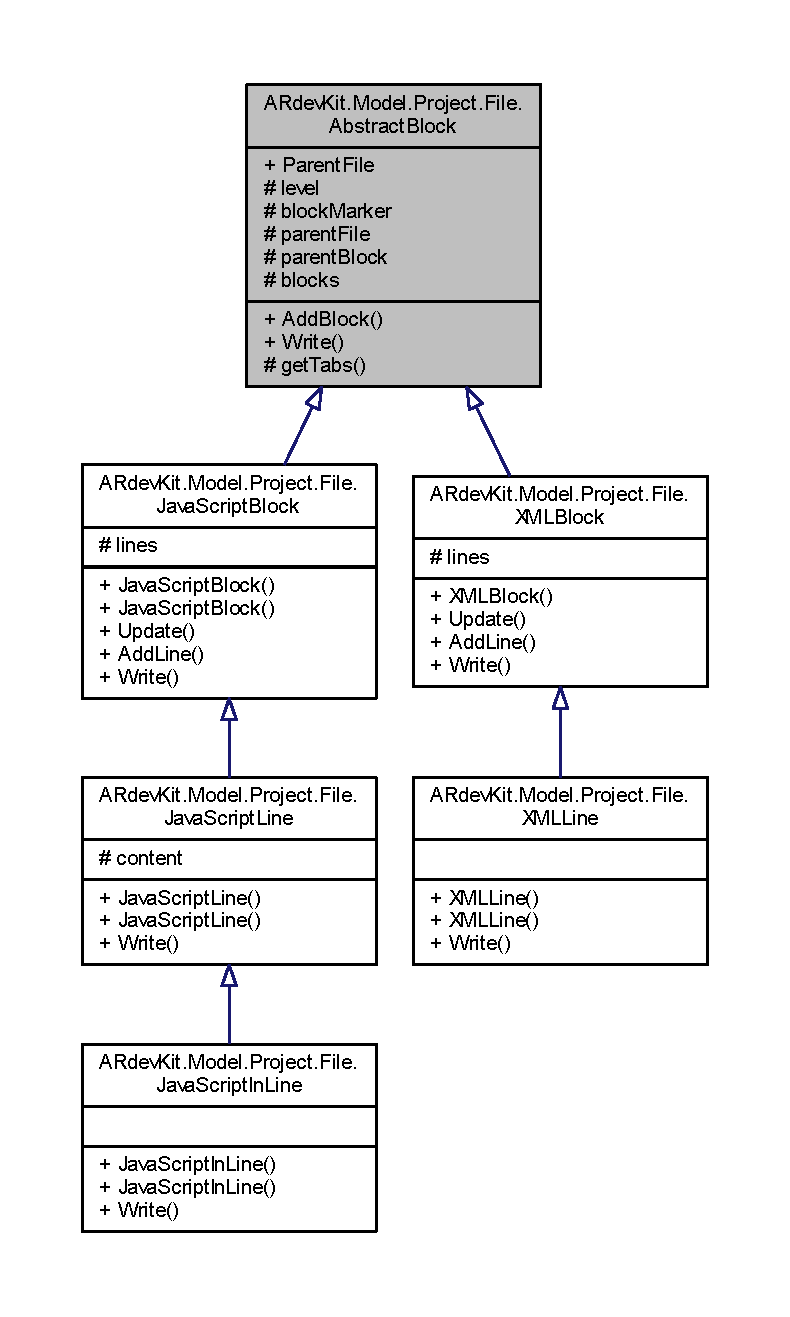
\includegraphics[height=550pt]{class_a_rdev_kit_1_1_model_1_1_project_1_1_file_1_1_abstract_block__inherit__graph}
\end{center}
\end{figure}


Collaboration diagram for A\-Rdev\-Kit.\-Model.\-Project.\-File.\-Abstract\-Block\-:
\nopagebreak
\begin{figure}[H]
\begin{center}
\leavevmode
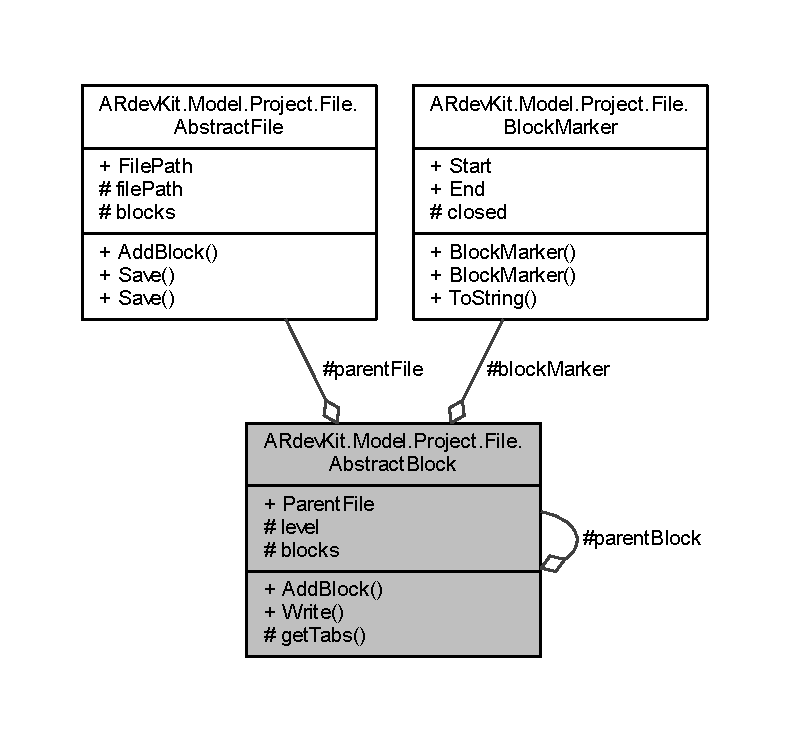
\includegraphics[width=350pt]{class_a_rdev_kit_1_1_model_1_1_project_1_1_file_1_1_abstract_block__coll__graph}
\end{center}
\end{figure}
\subsection*{Public Member Functions}
\begin{DoxyCompactItemize}
\item 
void \hyperlink{class_a_rdev_kit_1_1_model_1_1_project_1_1_file_1_1_abstract_block_aa238e4f3ad33fc75ab3741048ed4dc6b}{Add\-Block} (\hyperlink{class_a_rdev_kit_1_1_model_1_1_project_1_1_file_1_1_abstract_block}{Abstract\-Block} block)
\begin{DoxyCompactList}\small\item\em Adds an \hyperlink{class_a_rdev_kit_1_1_model_1_1_project_1_1_file_1_1_abstract_block}{Abstract\-Block}. \end{DoxyCompactList}\item 
virtual void \hyperlink{class_a_rdev_kit_1_1_model_1_1_project_1_1_file_1_1_abstract_block_a0b27a217de18a766c6647b71c41cc0ea}{Write} (System.\-I\-O.\-Stream\-Writer writer)
\begin{DoxyCompactList}\small\item\em Writes the \hyperlink{class_a_rdev_kit_1_1_model_1_1_project_1_1_file_1_1_abstract_block}{Abstract\-Block} with the given writer. \end{DoxyCompactList}\end{DoxyCompactItemize}
\subsection*{Protected Member Functions}
\begin{DoxyCompactItemize}
\item 
virtual string \hyperlink{class_a_rdev_kit_1_1_model_1_1_project_1_1_file_1_1_abstract_block_a851f696a88ce274c5f20e1c4bcbdef4c}{get\-Tabs} ()
\begin{DoxyCompactList}\small\item\em Returns a string containing \mbox{[}\hyperlink{class_a_rdev_kit_1_1_model_1_1_project_1_1_file_1_1_abstract_block_a7c07abfe27f2f9104fe7c3d23c7333a5}{level}\mbox{]} tabs. \end{DoxyCompactList}\end{DoxyCompactItemize}
\subsection*{Protected Attributes}
\begin{DoxyCompactItemize}
\item 
int \hyperlink{class_a_rdev_kit_1_1_model_1_1_project_1_1_file_1_1_abstract_block_a7c07abfe27f2f9104fe7c3d23c7333a5}{level}
\begin{DoxyCompactList}\small\item\em The level of the \hyperlink{class_a_rdev_kit_1_1_model_1_1_project_1_1_file_1_1_abstract_block}{Abstract\-Block}. \end{DoxyCompactList}\item 
\hyperlink{class_a_rdev_kit_1_1_model_1_1_project_1_1_file_1_1_block_marker}{Block\-Marker} \hyperlink{class_a_rdev_kit_1_1_model_1_1_project_1_1_file_1_1_abstract_block_a0975ceb65947c7370dcb6565677e9d0e}{block\-Marker}
\begin{DoxyCompactList}\small\item\em The \hyperlink{class_a_rdev_kit_1_1_model_1_1_project_1_1_file_1_1_block_marker}{Block\-Marker} of this \hyperlink{class_a_rdev_kit_1_1_model_1_1_project_1_1_file_1_1_abstract_block}{Abstract\-Block}. \end{DoxyCompactList}\item 
\hyperlink{class_a_rdev_kit_1_1_model_1_1_project_1_1_file_1_1_abstract_file}{Abstract\-File} \hyperlink{class_a_rdev_kit_1_1_model_1_1_project_1_1_file_1_1_abstract_block_a7dd07d5a865359c764a8cdab272a0662}{parent\-File}
\begin{DoxyCompactList}\small\item\em The \hyperlink{class_a_rdev_kit_1_1_model_1_1_project_1_1_file_1_1_abstract_file}{Abstract\-File} this block belongs to. \end{DoxyCompactList}\item 
\hyperlink{class_a_rdev_kit_1_1_model_1_1_project_1_1_file_1_1_abstract_block}{Abstract\-Block} \hyperlink{class_a_rdev_kit_1_1_model_1_1_project_1_1_file_1_1_abstract_block_aaa3372dadcd8d2b6ff2356ec984551c9}{parent\-Block}
\begin{DoxyCompactList}\small\item\em A \hyperlink{class_a_rdev_kit_1_1_model_1_1_project_1_1_file_1_1_abstract_block}{Abstract\-Block} this \hyperlink{class_a_rdev_kit_1_1_model_1_1_project_1_1_file_1_1_abstract_block}{Abstract\-Block} belongs to. \end{DoxyCompactList}\item 
List$<$ \hyperlink{class_a_rdev_kit_1_1_model_1_1_project_1_1_file_1_1_abstract_block}{Abstract\-Block} $>$ \hyperlink{class_a_rdev_kit_1_1_model_1_1_project_1_1_file_1_1_abstract_block_ae48e43536b76e45e5c84b837cc9bc093}{blocks}
\begin{DoxyCompactList}\small\item\em The \hyperlink{class_a_rdev_kit_1_1_model_1_1_project_1_1_file_1_1_abstract_block}{Abstract\-Block}s that belong to this \hyperlink{class_a_rdev_kit_1_1_model_1_1_project_1_1_file_1_1_abstract_block}{Abstract\-Block}. \end{DoxyCompactList}\end{DoxyCompactItemize}
\subsection*{Properties}
\begin{DoxyCompactItemize}
\item 
\hyperlink{class_a_rdev_kit_1_1_model_1_1_project_1_1_file_1_1_abstract_file}{Abstract\-File} \hyperlink{class_a_rdev_kit_1_1_model_1_1_project_1_1_file_1_1_abstract_block_a77fdd4b938d3f9d6d1f63e04018b4410}{Parent\-File}\hspace{0.3cm}{\ttfamily  \mbox{[}get, set\mbox{]}}
\begin{DoxyCompactList}\small\item\em Gets or sets the parent file. \end{DoxyCompactList}\end{DoxyCompactItemize}


\subsection{Detailed Description}
An \hyperlink{class_a_rdev_kit_1_1_model_1_1_project_1_1_file_1_1_abstract_block}{Abstract\-Block} has a \hyperlink{class_a_rdev_kit_1_1_model_1_1_project_1_1_file_1_1_abstract_block_a7c07abfe27f2f9104fe7c3d23c7333a5}{level} and can contain other \hyperlink{class_a_rdev_kit_1_1_model_1_1_project_1_1_file_1_1_abstract_block}{Abstract\-Block}s. It can have a \hyperlink{class_a_rdev_kit_1_1_model_1_1_project_1_1_file_1_1_block_marker}{Block\-Marker} and a \hyperlink{class_a_rdev_kit_1_1_model_1_1_project_1_1_file_1_1_abstract_block_a7dd07d5a865359c764a8cdab272a0662}{parent\-File}. 

Imanuel, 17.\-01.\-2014. 

\subsection{Member Function Documentation}
\hypertarget{class_a_rdev_kit_1_1_model_1_1_project_1_1_file_1_1_abstract_block_aa238e4f3ad33fc75ab3741048ed4dc6b}{\index{A\-Rdev\-Kit\-::\-Model\-::\-Project\-::\-File\-::\-Abstract\-Block@{A\-Rdev\-Kit\-::\-Model\-::\-Project\-::\-File\-::\-Abstract\-Block}!Add\-Block@{Add\-Block}}
\index{Add\-Block@{Add\-Block}!ARdevKit::Model::Project::File::AbstractBlock@{A\-Rdev\-Kit\-::\-Model\-::\-Project\-::\-File\-::\-Abstract\-Block}}
\subsubsection[{Add\-Block}]{\setlength{\rightskip}{0pt plus 5cm}void A\-Rdev\-Kit.\-Model.\-Project.\-File.\-Abstract\-Block.\-Add\-Block (
\begin{DoxyParamCaption}
\item[{{\bf Abstract\-Block}}]{block}
\end{DoxyParamCaption}
)}}\label{class_a_rdev_kit_1_1_model_1_1_project_1_1_file_1_1_abstract_block_aa238e4f3ad33fc75ab3741048ed4dc6b}


Adds an \hyperlink{class_a_rdev_kit_1_1_model_1_1_project_1_1_file_1_1_abstract_block}{Abstract\-Block}. 

Imanuel, 17.\-01.\-2014. 


\begin{DoxyParams}{Parameters}
{\em block} & The \hyperlink{class_a_rdev_kit_1_1_model_1_1_project_1_1_file_1_1_abstract_block}{Abstract\-Block}. \\
\hline
\end{DoxyParams}
\hypertarget{class_a_rdev_kit_1_1_model_1_1_project_1_1_file_1_1_abstract_block_a851f696a88ce274c5f20e1c4bcbdef4c}{\index{A\-Rdev\-Kit\-::\-Model\-::\-Project\-::\-File\-::\-Abstract\-Block@{A\-Rdev\-Kit\-::\-Model\-::\-Project\-::\-File\-::\-Abstract\-Block}!get\-Tabs@{get\-Tabs}}
\index{get\-Tabs@{get\-Tabs}!ARdevKit::Model::Project::File::AbstractBlock@{A\-Rdev\-Kit\-::\-Model\-::\-Project\-::\-File\-::\-Abstract\-Block}}
\subsubsection[{get\-Tabs}]{\setlength{\rightskip}{0pt plus 5cm}virtual string A\-Rdev\-Kit.\-Model.\-Project.\-File.\-Abstract\-Block.\-get\-Tabs (
\begin{DoxyParamCaption}
{}
\end{DoxyParamCaption}
)\hspace{0.3cm}{\ttfamily [protected]}, {\ttfamily [virtual]}}}\label{class_a_rdev_kit_1_1_model_1_1_project_1_1_file_1_1_abstract_block_a851f696a88ce274c5f20e1c4bcbdef4c}


Returns a string containing \mbox{[}\hyperlink{class_a_rdev_kit_1_1_model_1_1_project_1_1_file_1_1_abstract_block_a7c07abfe27f2f9104fe7c3d23c7333a5}{level}\mbox{]} tabs. 

Imanuel, 17.\-01.\-2014. 

\begin{DoxyReturn}{Returns}
The tabs. 
\end{DoxyReturn}
\hypertarget{class_a_rdev_kit_1_1_model_1_1_project_1_1_file_1_1_abstract_block_a0b27a217de18a766c6647b71c41cc0ea}{\index{A\-Rdev\-Kit\-::\-Model\-::\-Project\-::\-File\-::\-Abstract\-Block@{A\-Rdev\-Kit\-::\-Model\-::\-Project\-::\-File\-::\-Abstract\-Block}!Write@{Write}}
\index{Write@{Write}!ARdevKit::Model::Project::File::AbstractBlock@{A\-Rdev\-Kit\-::\-Model\-::\-Project\-::\-File\-::\-Abstract\-Block}}
\subsubsection[{Write}]{\setlength{\rightskip}{0pt plus 5cm}virtual void A\-Rdev\-Kit.\-Model.\-Project.\-File.\-Abstract\-Block.\-Write (
\begin{DoxyParamCaption}
\item[{System.\-I\-O.\-Stream\-Writer}]{writer}
\end{DoxyParamCaption}
)\hspace{0.3cm}{\ttfamily [virtual]}}}\label{class_a_rdev_kit_1_1_model_1_1_project_1_1_file_1_1_abstract_block_a0b27a217de18a766c6647b71c41cc0ea}


Writes the \hyperlink{class_a_rdev_kit_1_1_model_1_1_project_1_1_file_1_1_abstract_block}{Abstract\-Block} with the given writer. 

Imanuel, 15.\-01.\-2014. 


\begin{DoxyParams}{Parameters}
{\em writer} & The writer to write. \\
\hline
\end{DoxyParams}


Reimplemented in \hyperlink{class_a_rdev_kit_1_1_model_1_1_project_1_1_file_1_1_java_script_block_afe7251c8168c8d6062c7054bf0c21bf1}{A\-Rdev\-Kit.\-Model.\-Project.\-File.\-Java\-Script\-Block}, \hyperlink{class_a_rdev_kit_1_1_model_1_1_project_1_1_file_1_1_x_m_l_block_a93ad69ccbe004135c2cefca37e9f01db}{A\-Rdev\-Kit.\-Model.\-Project.\-File.\-X\-M\-L\-Block}, \hyperlink{class_a_rdev_kit_1_1_model_1_1_project_1_1_file_1_1_java_script_line_a9a1d47796fc64a50ccd602df70d1d562}{A\-Rdev\-Kit.\-Model.\-Project.\-File.\-Java\-Script\-Line}, \hyperlink{class_a_rdev_kit_1_1_model_1_1_project_1_1_file_1_1_java_script_in_line_a49f0664d2621cc8d5e0589c202c19b10}{A\-Rdev\-Kit.\-Model.\-Project.\-File.\-Java\-Script\-In\-Line}, and \hyperlink{class_a_rdev_kit_1_1_model_1_1_project_1_1_file_1_1_x_m_l_line_a7f58add9edb498bee39f2c09dc98c323}{A\-Rdev\-Kit.\-Model.\-Project.\-File.\-X\-M\-L\-Line}.



\subsection{Member Data Documentation}
\hypertarget{class_a_rdev_kit_1_1_model_1_1_project_1_1_file_1_1_abstract_block_a0975ceb65947c7370dcb6565677e9d0e}{\index{A\-Rdev\-Kit\-::\-Model\-::\-Project\-::\-File\-::\-Abstract\-Block@{A\-Rdev\-Kit\-::\-Model\-::\-Project\-::\-File\-::\-Abstract\-Block}!block\-Marker@{block\-Marker}}
\index{block\-Marker@{block\-Marker}!ARdevKit::Model::Project::File::AbstractBlock@{A\-Rdev\-Kit\-::\-Model\-::\-Project\-::\-File\-::\-Abstract\-Block}}
\subsubsection[{block\-Marker}]{\setlength{\rightskip}{0pt plus 5cm}{\bf Block\-Marker} A\-Rdev\-Kit.\-Model.\-Project.\-File.\-Abstract\-Block.\-block\-Marker\hspace{0.3cm}{\ttfamily [protected]}}}\label{class_a_rdev_kit_1_1_model_1_1_project_1_1_file_1_1_abstract_block_a0975ceb65947c7370dcb6565677e9d0e}


The \hyperlink{class_a_rdev_kit_1_1_model_1_1_project_1_1_file_1_1_block_marker}{Block\-Marker} of this \hyperlink{class_a_rdev_kit_1_1_model_1_1_project_1_1_file_1_1_abstract_block}{Abstract\-Block}. 

\hypertarget{class_a_rdev_kit_1_1_model_1_1_project_1_1_file_1_1_abstract_block_ae48e43536b76e45e5c84b837cc9bc093}{\index{A\-Rdev\-Kit\-::\-Model\-::\-Project\-::\-File\-::\-Abstract\-Block@{A\-Rdev\-Kit\-::\-Model\-::\-Project\-::\-File\-::\-Abstract\-Block}!blocks@{blocks}}
\index{blocks@{blocks}!ARdevKit::Model::Project::File::AbstractBlock@{A\-Rdev\-Kit\-::\-Model\-::\-Project\-::\-File\-::\-Abstract\-Block}}
\subsubsection[{blocks}]{\setlength{\rightskip}{0pt plus 5cm}List$<${\bf Abstract\-Block}$>$ A\-Rdev\-Kit.\-Model.\-Project.\-File.\-Abstract\-Block.\-blocks\hspace{0.3cm}{\ttfamily [protected]}}}\label{class_a_rdev_kit_1_1_model_1_1_project_1_1_file_1_1_abstract_block_ae48e43536b76e45e5c84b837cc9bc093}


The \hyperlink{class_a_rdev_kit_1_1_model_1_1_project_1_1_file_1_1_abstract_block}{Abstract\-Block}s that belong to this \hyperlink{class_a_rdev_kit_1_1_model_1_1_project_1_1_file_1_1_abstract_block}{Abstract\-Block}. 

\hypertarget{class_a_rdev_kit_1_1_model_1_1_project_1_1_file_1_1_abstract_block_a7c07abfe27f2f9104fe7c3d23c7333a5}{\index{A\-Rdev\-Kit\-::\-Model\-::\-Project\-::\-File\-::\-Abstract\-Block@{A\-Rdev\-Kit\-::\-Model\-::\-Project\-::\-File\-::\-Abstract\-Block}!level@{level}}
\index{level@{level}!ARdevKit::Model::Project::File::AbstractBlock@{A\-Rdev\-Kit\-::\-Model\-::\-Project\-::\-File\-::\-Abstract\-Block}}
\subsubsection[{level}]{\setlength{\rightskip}{0pt plus 5cm}int A\-Rdev\-Kit.\-Model.\-Project.\-File.\-Abstract\-Block.\-level\hspace{0.3cm}{\ttfamily [protected]}}}\label{class_a_rdev_kit_1_1_model_1_1_project_1_1_file_1_1_abstract_block_a7c07abfe27f2f9104fe7c3d23c7333a5}


The level of the \hyperlink{class_a_rdev_kit_1_1_model_1_1_project_1_1_file_1_1_abstract_block}{Abstract\-Block}. 

The level. \hypertarget{class_a_rdev_kit_1_1_model_1_1_project_1_1_file_1_1_abstract_block_aaa3372dadcd8d2b6ff2356ec984551c9}{\index{A\-Rdev\-Kit\-::\-Model\-::\-Project\-::\-File\-::\-Abstract\-Block@{A\-Rdev\-Kit\-::\-Model\-::\-Project\-::\-File\-::\-Abstract\-Block}!parent\-Block@{parent\-Block}}
\index{parent\-Block@{parent\-Block}!ARdevKit::Model::Project::File::AbstractBlock@{A\-Rdev\-Kit\-::\-Model\-::\-Project\-::\-File\-::\-Abstract\-Block}}
\subsubsection[{parent\-Block}]{\setlength{\rightskip}{0pt plus 5cm}{\bf Abstract\-Block} A\-Rdev\-Kit.\-Model.\-Project.\-File.\-Abstract\-Block.\-parent\-Block\hspace{0.3cm}{\ttfamily [protected]}}}\label{class_a_rdev_kit_1_1_model_1_1_project_1_1_file_1_1_abstract_block_aaa3372dadcd8d2b6ff2356ec984551c9}


A \hyperlink{class_a_rdev_kit_1_1_model_1_1_project_1_1_file_1_1_abstract_block}{Abstract\-Block} this \hyperlink{class_a_rdev_kit_1_1_model_1_1_project_1_1_file_1_1_abstract_block}{Abstract\-Block} belongs to. 

\hypertarget{class_a_rdev_kit_1_1_model_1_1_project_1_1_file_1_1_abstract_block_a7dd07d5a865359c764a8cdab272a0662}{\index{A\-Rdev\-Kit\-::\-Model\-::\-Project\-::\-File\-::\-Abstract\-Block@{A\-Rdev\-Kit\-::\-Model\-::\-Project\-::\-File\-::\-Abstract\-Block}!parent\-File@{parent\-File}}
\index{parent\-File@{parent\-File}!ARdevKit::Model::Project::File::AbstractBlock@{A\-Rdev\-Kit\-::\-Model\-::\-Project\-::\-File\-::\-Abstract\-Block}}
\subsubsection[{parent\-File}]{\setlength{\rightskip}{0pt plus 5cm}{\bf Abstract\-File} A\-Rdev\-Kit.\-Model.\-Project.\-File.\-Abstract\-Block.\-parent\-File\hspace{0.3cm}{\ttfamily [protected]}}}\label{class_a_rdev_kit_1_1_model_1_1_project_1_1_file_1_1_abstract_block_a7dd07d5a865359c764a8cdab272a0662}


The \hyperlink{class_a_rdev_kit_1_1_model_1_1_project_1_1_file_1_1_abstract_file}{Abstract\-File} this block belongs to. 



\subsection{Property Documentation}
\hypertarget{class_a_rdev_kit_1_1_model_1_1_project_1_1_file_1_1_abstract_block_a77fdd4b938d3f9d6d1f63e04018b4410}{\index{A\-Rdev\-Kit\-::\-Model\-::\-Project\-::\-File\-::\-Abstract\-Block@{A\-Rdev\-Kit\-::\-Model\-::\-Project\-::\-File\-::\-Abstract\-Block}!Parent\-File@{Parent\-File}}
\index{Parent\-File@{Parent\-File}!ARdevKit::Model::Project::File::AbstractBlock@{A\-Rdev\-Kit\-::\-Model\-::\-Project\-::\-File\-::\-Abstract\-Block}}
\subsubsection[{Parent\-File}]{\setlength{\rightskip}{0pt plus 5cm}{\bf Abstract\-File} A\-Rdev\-Kit.\-Model.\-Project.\-File.\-Abstract\-Block.\-Parent\-File\hspace{0.3cm}{\ttfamily [get]}, {\ttfamily [set]}}}\label{class_a_rdev_kit_1_1_model_1_1_project_1_1_file_1_1_abstract_block_a77fdd4b938d3f9d6d1f63e04018b4410}


Gets or sets the parent file. 

The parent file. 
\hypertarget{class_a_rdev_kit_1_1_model_1_1_project_1_1_abstract_dynamic2_d_augmentation}{\section{A\-Rdev\-Kit.\-Model.\-Project.\-Abstract\-Dynamic2\-D\-Augmentation Class Reference}
\label{class_a_rdev_kit_1_1_model_1_1_project_1_1_abstract_dynamic2_d_augmentation}\index{A\-Rdev\-Kit.\-Model.\-Project.\-Abstract\-Dynamic2\-D\-Augmentation@{A\-Rdev\-Kit.\-Model.\-Project.\-Abstract\-Dynamic2\-D\-Augmentation}}
}


Inherits from \hyperlink{class_a_rdev_kit_1_1_model_1_1_project_1_1_abstract2_d_augmentation}{Abstract2\-D\-Augmentation} and adds \hyperlink{class_a_rdev_kit_1_1_model_1_1_project_1_1_abstract_source}{Abstract\-Source}, in order to show dynamic content.  




Inheritance diagram for A\-Rdev\-Kit.\-Model.\-Project.\-Abstract\-Dynamic2\-D\-Augmentation\-:
\nopagebreak
\begin{figure}[H]
\begin{center}
\leavevmode
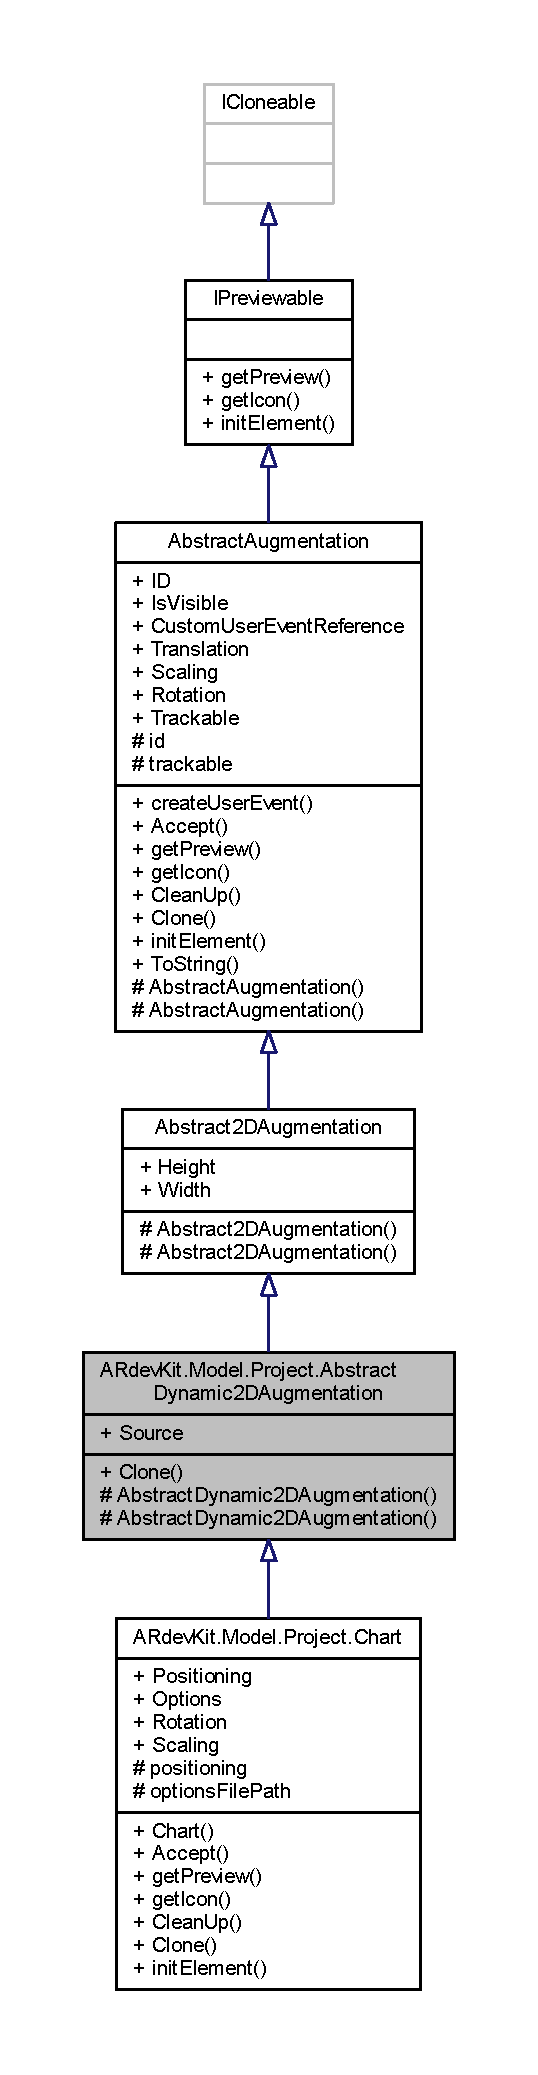
\includegraphics[height=550pt]{class_a_rdev_kit_1_1_model_1_1_project_1_1_abstract_dynamic2_d_augmentation__inherit__graph}
\end{center}
\end{figure}


Collaboration diagram for A\-Rdev\-Kit.\-Model.\-Project.\-Abstract\-Dynamic2\-D\-Augmentation\-:
\nopagebreak
\begin{figure}[H]
\begin{center}
\leavevmode
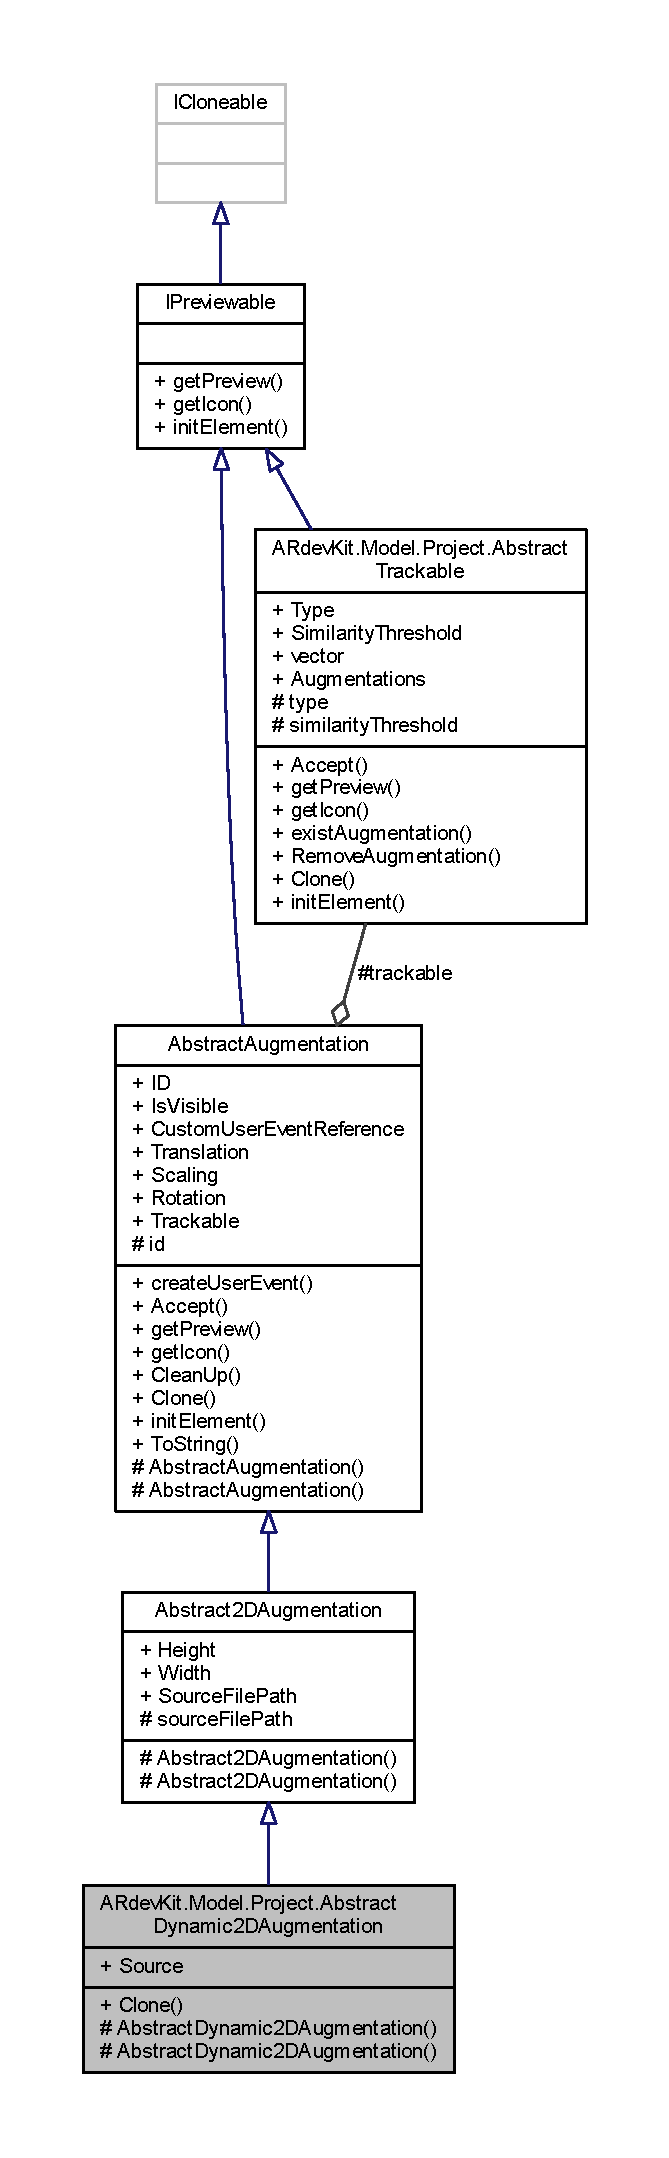
\includegraphics[height=550pt]{class_a_rdev_kit_1_1_model_1_1_project_1_1_abstract_dynamic2_d_augmentation__coll__graph}
\end{center}
\end{figure}
\subsection*{Public Member Functions}
\begin{DoxyCompactItemize}
\item 
override object \hyperlink{class_a_rdev_kit_1_1_model_1_1_project_1_1_abstract_dynamic2_d_augmentation_adbb2d06450362f0385fe937bbb5255a8}{Clone} ()
\begin{DoxyCompactList}\small\item\em Makes a deep copy of this object. \end{DoxyCompactList}\end{DoxyCompactItemize}
\subsection*{Protected Member Functions}
\begin{DoxyCompactItemize}
\item 
\hyperlink{class_a_rdev_kit_1_1_model_1_1_project_1_1_abstract_dynamic2_d_augmentation_aacdc5a86b00f5fdf9e86ca8060c8b5e1}{Abstract\-Dynamic2\-D\-Augmentation} ()
\begin{DoxyCompactList}\small\item\em Initializes no new instance of the \hyperlink{class_a_rdev_kit_1_1_model_1_1_project_1_1_abstract_dynamic2_d_augmentation}{Abstract\-Dynamic2\-D\-Augmentation} class, but can be used by inheriting classes. It is using the standard constructor from \hyperlink{class_a_rdev_kit_1_1_model_1_1_project_1_1_abstract2_d_augmentation}{Abstract2\-D\-Augmentation}. \end{DoxyCompactList}\item 
\hyperlink{class_a_rdev_kit_1_1_model_1_1_project_1_1_abstract_dynamic2_d_augmentation_ab0861137122d08818a2df5c6e787e848}{Abstract\-Dynamic2\-D\-Augmentation} (bool is\-Visible, \hyperlink{class_a_rdev_kit_1_1_model_1_1_project_1_1_vector3_d}{Vector3\-D} translation\-Vector, \hyperlink{class_a_rdev_kit_1_1_model_1_1_project_1_1_vector3_d}{Vector3\-D} scaling, \hyperlink{class_a_rdev_kit_1_1_model_1_1_project_1_1_abstract_trackable}{Abstract\-Trackable} \hyperlink{class_a_rdev_kit_1_1_model_1_1_project_1_1_abstract_augmentation_a8d8e3f3c42696008edbfc44d51ba518d}{trackable}, int width, int height, \hyperlink{class_a_rdev_kit_1_1_model_1_1_project_1_1_abstract_source}{Abstract\-Source} source)
\begin{DoxyCompactList}\small\item\em Initializes no new instance of the \hyperlink{class_a_rdev_kit_1_1_model_1_1_project_1_1_abstract_dynamic2_d_augmentation}{Abstract\-Dynamic2\-D\-Augmentation} class, but can be used by inheriting classes. It is using the constructor from \hyperlink{class_a_rdev_kit_1_1_model_1_1_project_1_1_abstract2_d_augmentation}{Abstract2\-D\-Augmentation}. \end{DoxyCompactList}\end{DoxyCompactItemize}
\subsection*{Properties}
\begin{DoxyCompactItemize}
\item 
\hyperlink{class_a_rdev_kit_1_1_model_1_1_project_1_1_abstract_source}{Abstract\-Source} \hyperlink{class_a_rdev_kit_1_1_model_1_1_project_1_1_abstract_dynamic2_d_augmentation_a6abf4f1aff81779f1ec989c2cb99bdf3}{Source}\hspace{0.3cm}{\ttfamily  \mbox{[}get, set\mbox{]}}
\begin{DoxyCompactList}\small\item\em variable which links an \hyperlink{class_a_rdev_kit_1_1_model_1_1_project_1_1_abstract_source}{Abstract\-Source} to this \hyperlink{class_a_rdev_kit_1_1_model_1_1_project_1_1_abstract2_d_augmentation}{Abstract2\-D\-Augmentation}. \end{DoxyCompactList}\end{DoxyCompactItemize}
\subsection*{Additional Inherited Members}


\subsection{Detailed Description}
Inherits from \hyperlink{class_a_rdev_kit_1_1_model_1_1_project_1_1_abstract2_d_augmentation}{Abstract2\-D\-Augmentation} and adds \hyperlink{class_a_rdev_kit_1_1_model_1_1_project_1_1_abstract_source}{Abstract\-Source}, in order to show dynamic content. 



\subsection{Constructor \& Destructor Documentation}
\hypertarget{class_a_rdev_kit_1_1_model_1_1_project_1_1_abstract_dynamic2_d_augmentation_aacdc5a86b00f5fdf9e86ca8060c8b5e1}{\index{A\-Rdev\-Kit\-::\-Model\-::\-Project\-::\-Abstract\-Dynamic2\-D\-Augmentation@{A\-Rdev\-Kit\-::\-Model\-::\-Project\-::\-Abstract\-Dynamic2\-D\-Augmentation}!Abstract\-Dynamic2\-D\-Augmentation@{Abstract\-Dynamic2\-D\-Augmentation}}
\index{Abstract\-Dynamic2\-D\-Augmentation@{Abstract\-Dynamic2\-D\-Augmentation}!ARdevKit::Model::Project::AbstractDynamic2DAugmentation@{A\-Rdev\-Kit\-::\-Model\-::\-Project\-::\-Abstract\-Dynamic2\-D\-Augmentation}}
\subsubsection[{Abstract\-Dynamic2\-D\-Augmentation}]{\setlength{\rightskip}{0pt plus 5cm}A\-Rdev\-Kit.\-Model.\-Project.\-Abstract\-Dynamic2\-D\-Augmentation.\-Abstract\-Dynamic2\-D\-Augmentation (
\begin{DoxyParamCaption}
{}
\end{DoxyParamCaption}
)\hspace{0.3cm}{\ttfamily [protected]}}}\label{class_a_rdev_kit_1_1_model_1_1_project_1_1_abstract_dynamic2_d_augmentation_aacdc5a86b00f5fdf9e86ca8060c8b5e1}


Initializes no new instance of the \hyperlink{class_a_rdev_kit_1_1_model_1_1_project_1_1_abstract_dynamic2_d_augmentation}{Abstract\-Dynamic2\-D\-Augmentation} class, but can be used by inheriting classes. It is using the standard constructor from \hyperlink{class_a_rdev_kit_1_1_model_1_1_project_1_1_abstract2_d_augmentation}{Abstract2\-D\-Augmentation}. 

\hypertarget{class_a_rdev_kit_1_1_model_1_1_project_1_1_abstract_dynamic2_d_augmentation_ab0861137122d08818a2df5c6e787e848}{\index{A\-Rdev\-Kit\-::\-Model\-::\-Project\-::\-Abstract\-Dynamic2\-D\-Augmentation@{A\-Rdev\-Kit\-::\-Model\-::\-Project\-::\-Abstract\-Dynamic2\-D\-Augmentation}!Abstract\-Dynamic2\-D\-Augmentation@{Abstract\-Dynamic2\-D\-Augmentation}}
\index{Abstract\-Dynamic2\-D\-Augmentation@{Abstract\-Dynamic2\-D\-Augmentation}!ARdevKit::Model::Project::AbstractDynamic2DAugmentation@{A\-Rdev\-Kit\-::\-Model\-::\-Project\-::\-Abstract\-Dynamic2\-D\-Augmentation}}
\subsubsection[{Abstract\-Dynamic2\-D\-Augmentation}]{\setlength{\rightskip}{0pt plus 5cm}A\-Rdev\-Kit.\-Model.\-Project.\-Abstract\-Dynamic2\-D\-Augmentation.\-Abstract\-Dynamic2\-D\-Augmentation (
\begin{DoxyParamCaption}
\item[{bool}]{is\-Visible, }
\item[{{\bf Vector3\-D}}]{translation\-Vector, }
\item[{{\bf Vector3\-D}}]{scaling, }
\item[{{\bf Abstract\-Trackable}}]{trackable, }
\item[{int}]{width, }
\item[{int}]{height, }
\item[{{\bf Abstract\-Source}}]{source}
\end{DoxyParamCaption}
)\hspace{0.3cm}{\ttfamily [protected]}}}\label{class_a_rdev_kit_1_1_model_1_1_project_1_1_abstract_dynamic2_d_augmentation_ab0861137122d08818a2df5c6e787e848}


Initializes no new instance of the \hyperlink{class_a_rdev_kit_1_1_model_1_1_project_1_1_abstract_dynamic2_d_augmentation}{Abstract\-Dynamic2\-D\-Augmentation} class, but can be used by inheriting classes. It is using the constructor from \hyperlink{class_a_rdev_kit_1_1_model_1_1_project_1_1_abstract2_d_augmentation}{Abstract2\-D\-Augmentation}. 


\begin{DoxyParams}{Parameters}
{\em is\-Visible} & if set to {\ttfamily true} \mbox{[}is visible\mbox{]} using A\-R\-E\-L.\\
\hline
{\em translation\-Vector} & The translation vector.\\
\hline
{\em scaling} & The scaling.\\
\hline
{\em trackable} & The trackable.\\
\hline
{\em width} & The width.\\
\hline
{\em height} & The height.\\
\hline
{\em source} & The source.\\
\hline
\end{DoxyParams}


\subsection{Member Function Documentation}
\hypertarget{class_a_rdev_kit_1_1_model_1_1_project_1_1_abstract_dynamic2_d_augmentation_adbb2d06450362f0385fe937bbb5255a8}{\index{A\-Rdev\-Kit\-::\-Model\-::\-Project\-::\-Abstract\-Dynamic2\-D\-Augmentation@{A\-Rdev\-Kit\-::\-Model\-::\-Project\-::\-Abstract\-Dynamic2\-D\-Augmentation}!Clone@{Clone}}
\index{Clone@{Clone}!ARdevKit::Model::Project::AbstractDynamic2DAugmentation@{A\-Rdev\-Kit\-::\-Model\-::\-Project\-::\-Abstract\-Dynamic2\-D\-Augmentation}}
\subsubsection[{Clone}]{\setlength{\rightskip}{0pt plus 5cm}override object A\-Rdev\-Kit.\-Model.\-Project.\-Abstract\-Dynamic2\-D\-Augmentation.\-Clone (
\begin{DoxyParamCaption}
{}
\end{DoxyParamCaption}
)\hspace{0.3cm}{\ttfamily [virtual]}}}\label{class_a_rdev_kit_1_1_model_1_1_project_1_1_abstract_dynamic2_d_augmentation_adbb2d06450362f0385fe937bbb5255a8}


Makes a deep copy of this object. 

Robin, 30.\-01.\-2014. 

\begin{DoxyReturn}{Returns}
A copy of this object. 
\end{DoxyReturn}


Implements \hyperlink{class_a_rdev_kit_1_1_model_1_1_project_1_1_abstract_augmentation_a184416a3d47e35d58bb7f5bb6ce2e269}{A\-Rdev\-Kit.\-Model.\-Project.\-Abstract\-Augmentation}.



Reimplemented in \hyperlink{class_a_rdev_kit_1_1_model_1_1_project_1_1_chart_aaa06b6e53f2e5a48508f3a93b0483dc3}{A\-Rdev\-Kit.\-Model.\-Project.\-Chart}.



\subsection{Property Documentation}
\hypertarget{class_a_rdev_kit_1_1_model_1_1_project_1_1_abstract_dynamic2_d_augmentation_a6abf4f1aff81779f1ec989c2cb99bdf3}{\index{A\-Rdev\-Kit\-::\-Model\-::\-Project\-::\-Abstract\-Dynamic2\-D\-Augmentation@{A\-Rdev\-Kit\-::\-Model\-::\-Project\-::\-Abstract\-Dynamic2\-D\-Augmentation}!Source@{Source}}
\index{Source@{Source}!ARdevKit::Model::Project::AbstractDynamic2DAugmentation@{A\-Rdev\-Kit\-::\-Model\-::\-Project\-::\-Abstract\-Dynamic2\-D\-Augmentation}}
\subsubsection[{Source}]{\setlength{\rightskip}{0pt plus 5cm}{\bf Abstract\-Source} A\-Rdev\-Kit.\-Model.\-Project.\-Abstract\-Dynamic2\-D\-Augmentation.\-Source\hspace{0.3cm}{\ttfamily [get]}, {\ttfamily [set]}}}\label{class_a_rdev_kit_1_1_model_1_1_project_1_1_abstract_dynamic2_d_augmentation_a6abf4f1aff81779f1ec989c2cb99bdf3}


variable which links an \hyperlink{class_a_rdev_kit_1_1_model_1_1_project_1_1_abstract_source}{Abstract\-Source} to this \hyperlink{class_a_rdev_kit_1_1_model_1_1_project_1_1_abstract2_d_augmentation}{Abstract2\-D\-Augmentation}. 


\hypertarget{class_a_rdev_kit_1_1_model_1_1_project_1_1_file_1_1_abstract_file}{\section{A\-Rdev\-Kit.\-Model.\-Project.\-File.\-Abstract\-File Class Reference}
\label{class_a_rdev_kit_1_1_model_1_1_project_1_1_file_1_1_abstract_file}\index{A\-Rdev\-Kit.\-Model.\-Project.\-File.\-Abstract\-File@{A\-Rdev\-Kit.\-Model.\-Project.\-File.\-Abstract\-File}}
}


An \hyperlink{class_a_rdev_kit_1_1_model_1_1_project_1_1_file_1_1_abstract_file}{Abstract\-File} can be an \hyperlink{class_a_rdev_kit_1_1_model_1_1_project_1_1_file_1_1_a_r_e_l_config_file}{A\-R\-E\-L\-Config\-File}, an \hyperlink{class_a_rdev_kit_1_1_model_1_1_project_1_1_file_1_1_a_r_e_l_project_file}{A\-R\-E\-L\-Project\-File}, a Trackin\-Data\-File or an \hyperlink{class_a_rdev_kit_1_1_model_1_1_project_1_1_file_1_1_a_r_e_l_glue_file}{A\-R\-E\-L\-Glue\-File}. It must have a \hyperlink{class_a_rdev_kit_1_1_model_1_1_project_1_1_file_1_1_abstract_file_ad879e3a81860da8b72f2d9f61a18ab3b}{file\-Path} and can have a header and consists of \hyperlink{class_a_rdev_kit_1_1_model_1_1_project_1_1_file_1_1_abstract_block}{Abstract\-Block}s.  




Inheritance diagram for A\-Rdev\-Kit.\-Model.\-Project.\-File.\-Abstract\-File\-:
\nopagebreak
\begin{figure}[H]
\begin{center}
\leavevmode
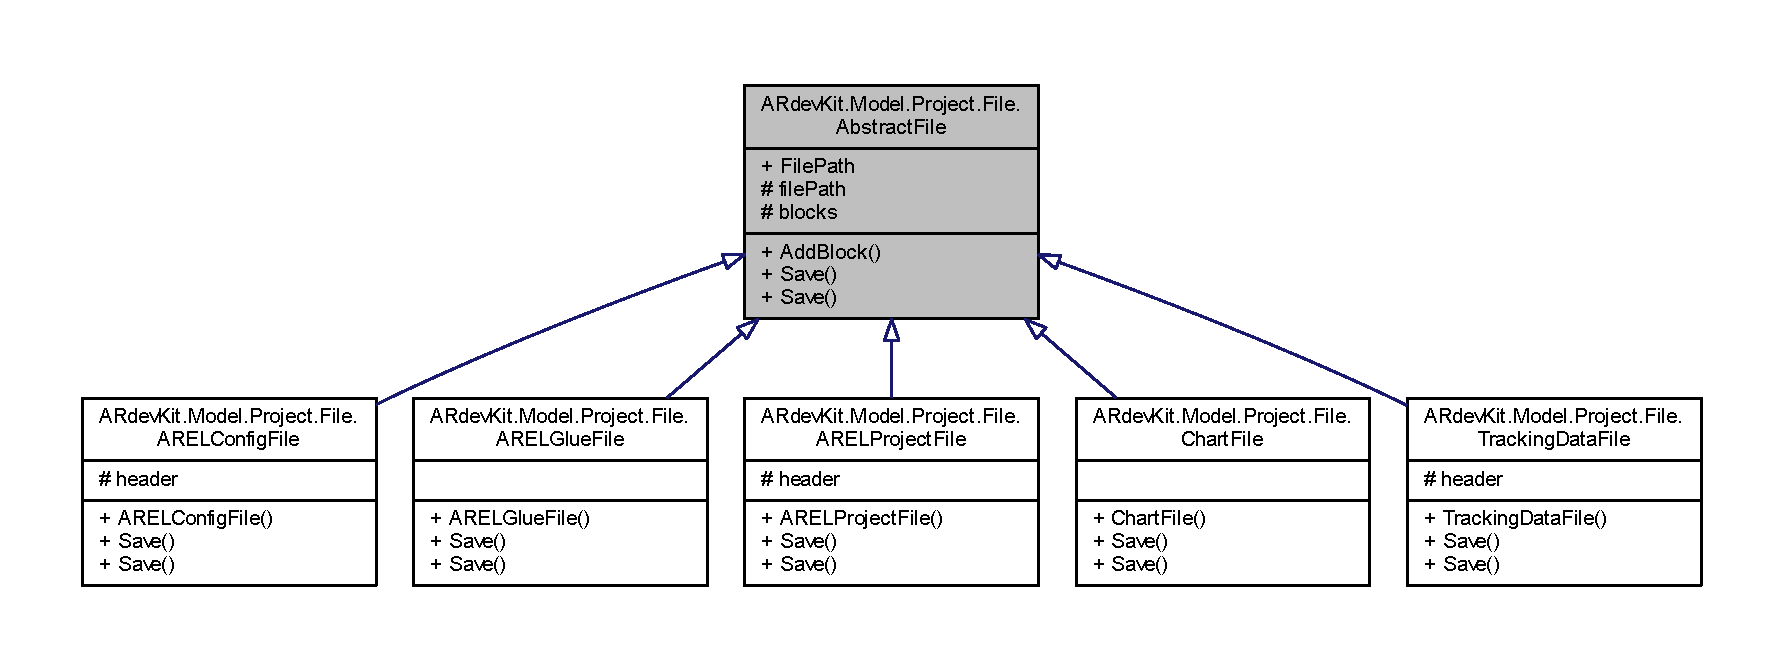
\includegraphics[width=350pt]{class_a_rdev_kit_1_1_model_1_1_project_1_1_file_1_1_abstract_file__inherit__graph}
\end{center}
\end{figure}


Collaboration diagram for A\-Rdev\-Kit.\-Model.\-Project.\-File.\-Abstract\-File\-:
\nopagebreak
\begin{figure}[H]
\begin{center}
\leavevmode
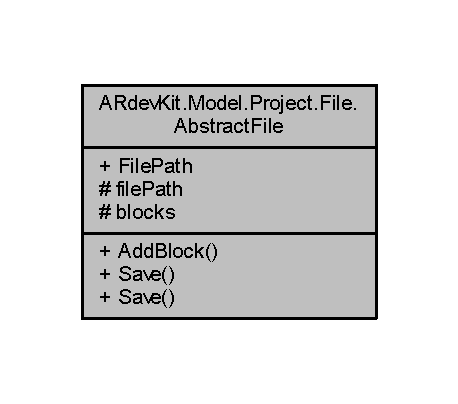
\includegraphics[width=220pt]{class_a_rdev_kit_1_1_model_1_1_project_1_1_file_1_1_abstract_file__coll__graph}
\end{center}
\end{figure}
\subsection*{Public Member Functions}
\begin{DoxyCompactItemize}
\item 
virtual void \hyperlink{class_a_rdev_kit_1_1_model_1_1_project_1_1_file_1_1_abstract_file_a02b61dbebfbd57f5fd44c7a972c79b50}{Add\-Block} (\hyperlink{class_a_rdev_kit_1_1_model_1_1_project_1_1_file_1_1_abstract_block}{Abstract\-Block} block)
\begin{DoxyCompactList}\small\item\em Adds an \hyperlink{class_a_rdev_kit_1_1_model_1_1_project_1_1_file_1_1_abstract_block}{Abstract\-Block}. \end{DoxyCompactList}\item 
abstract void \hyperlink{class_a_rdev_kit_1_1_model_1_1_project_1_1_file_1_1_abstract_file_ae49c3262c59642e8f519d0655bbbbbab}{Save} (string project\-Path)
\begin{DoxyCompactList}\small\item\em Saves the file to the using the passed project\-Path. \end{DoxyCompactList}\item 
abstract void \hyperlink{class_a_rdev_kit_1_1_model_1_1_project_1_1_file_1_1_abstract_file_a095ebaeca96a6d285d9caff1ad726d5b}{Save} ()
\begin{DoxyCompactList}\small\item\em Saves the file to its \hyperlink{class_a_rdev_kit_1_1_model_1_1_project_1_1_file_1_1_abstract_file_ad879e3a81860da8b72f2d9f61a18ab3b}{file\-Path}. \end{DoxyCompactList}\end{DoxyCompactItemize}
\subsection*{Protected Attributes}
\begin{DoxyCompactItemize}
\item 
string \hyperlink{class_a_rdev_kit_1_1_model_1_1_project_1_1_file_1_1_abstract_file_ad879e3a81860da8b72f2d9f61a18ab3b}{file\-Path}
\begin{DoxyCompactList}\small\item\em Full pathname of the file. \end{DoxyCompactList}\item 
List$<$ \hyperlink{class_a_rdev_kit_1_1_model_1_1_project_1_1_file_1_1_abstract_block}{Abstract\-Block} $>$ \hyperlink{class_a_rdev_kit_1_1_model_1_1_project_1_1_file_1_1_abstract_file_a21e0333fb9d8eab8ebb039bd56ccabc9}{blocks}
\begin{DoxyCompactList}\small\item\em A list of the \hyperlink{class_a_rdev_kit_1_1_model_1_1_project_1_1_file_1_1_abstract_block}{Abstract\-Block}s this file consists of. \end{DoxyCompactList}\end{DoxyCompactItemize}
\subsection*{Properties}
\begin{DoxyCompactItemize}
\item 
string \hyperlink{class_a_rdev_kit_1_1_model_1_1_project_1_1_file_1_1_abstract_file_ac55b0e087f42f7ab5ce36fa3bce111ab}{File\-Path}\hspace{0.3cm}{\ttfamily  \mbox{[}get\mbox{]}}
\begin{DoxyCompactList}\small\item\em Gets the full pathname of the file. \end{DoxyCompactList}\end{DoxyCompactItemize}


\subsection{Detailed Description}
An \hyperlink{class_a_rdev_kit_1_1_model_1_1_project_1_1_file_1_1_abstract_file}{Abstract\-File} can be an \hyperlink{class_a_rdev_kit_1_1_model_1_1_project_1_1_file_1_1_a_r_e_l_config_file}{A\-R\-E\-L\-Config\-File}, an \hyperlink{class_a_rdev_kit_1_1_model_1_1_project_1_1_file_1_1_a_r_e_l_project_file}{A\-R\-E\-L\-Project\-File}, a Trackin\-Data\-File or an \hyperlink{class_a_rdev_kit_1_1_model_1_1_project_1_1_file_1_1_a_r_e_l_glue_file}{A\-R\-E\-L\-Glue\-File}. It must have a \hyperlink{class_a_rdev_kit_1_1_model_1_1_project_1_1_file_1_1_abstract_file_ad879e3a81860da8b72f2d9f61a18ab3b}{file\-Path} and can have a header and consists of \hyperlink{class_a_rdev_kit_1_1_model_1_1_project_1_1_file_1_1_abstract_block}{Abstract\-Block}s. 

Imanuel, 15.\-01.\-2014. 

\subsection{Member Function Documentation}
\hypertarget{class_a_rdev_kit_1_1_model_1_1_project_1_1_file_1_1_abstract_file_a02b61dbebfbd57f5fd44c7a972c79b50}{\index{A\-Rdev\-Kit\-::\-Model\-::\-Project\-::\-File\-::\-Abstract\-File@{A\-Rdev\-Kit\-::\-Model\-::\-Project\-::\-File\-::\-Abstract\-File}!Add\-Block@{Add\-Block}}
\index{Add\-Block@{Add\-Block}!ARdevKit::Model::Project::File::AbstractFile@{A\-Rdev\-Kit\-::\-Model\-::\-Project\-::\-File\-::\-Abstract\-File}}
\subsubsection[{Add\-Block}]{\setlength{\rightskip}{0pt plus 5cm}virtual void A\-Rdev\-Kit.\-Model.\-Project.\-File.\-Abstract\-File.\-Add\-Block (
\begin{DoxyParamCaption}
\item[{{\bf Abstract\-Block}}]{block}
\end{DoxyParamCaption}
)\hspace{0.3cm}{\ttfamily [virtual]}}}\label{class_a_rdev_kit_1_1_model_1_1_project_1_1_file_1_1_abstract_file_a02b61dbebfbd57f5fd44c7a972c79b50}


Adds an \hyperlink{class_a_rdev_kit_1_1_model_1_1_project_1_1_file_1_1_abstract_block}{Abstract\-Block}. 

Imanuel, 15.\-01.\-2014. 


\begin{DoxyParams}{Parameters}
{\em block} & The section to be added. \\
\hline
\end{DoxyParams}
\hypertarget{class_a_rdev_kit_1_1_model_1_1_project_1_1_file_1_1_abstract_file_ae49c3262c59642e8f519d0655bbbbbab}{\index{A\-Rdev\-Kit\-::\-Model\-::\-Project\-::\-File\-::\-Abstract\-File@{A\-Rdev\-Kit\-::\-Model\-::\-Project\-::\-File\-::\-Abstract\-File}!Save@{Save}}
\index{Save@{Save}!ARdevKit::Model::Project::File::AbstractFile@{A\-Rdev\-Kit\-::\-Model\-::\-Project\-::\-File\-::\-Abstract\-File}}
\subsubsection[{Save}]{\setlength{\rightskip}{0pt plus 5cm}abstract void A\-Rdev\-Kit.\-Model.\-Project.\-File.\-Abstract\-File.\-Save (
\begin{DoxyParamCaption}
\item[{string}]{project\-Path}
\end{DoxyParamCaption}
)\hspace{0.3cm}{\ttfamily [pure virtual]}}}\label{class_a_rdev_kit_1_1_model_1_1_project_1_1_file_1_1_abstract_file_ae49c3262c59642e8f519d0655bbbbbab}


Saves the file to the using the passed project\-Path. 

Imanuel, 15.\-01.\-2014. 


\begin{DoxyParams}{Parameters}
{\em project\-Path} & The project path to write. \\
\hline
\end{DoxyParams}


Implemented in \hyperlink{class_a_rdev_kit_1_1_model_1_1_project_1_1_file_1_1_tracking_data_file_a6b96d140f6a8e9c98888afece89b41f5}{A\-Rdev\-Kit.\-Model.\-Project.\-File.\-Tracking\-Data\-File}, \hyperlink{class_a_rdev_kit_1_1_model_1_1_project_1_1_file_1_1_a_r_e_l_config_file_af0f2e70451d0dda0984dd186fcb6afde}{A\-Rdev\-Kit.\-Model.\-Project.\-File.\-A\-R\-E\-L\-Config\-File}, \hyperlink{class_a_rdev_kit_1_1_model_1_1_project_1_1_file_1_1_a_r_e_l_project_file_aa187897624d6d836b3a76331069d5bee}{A\-Rdev\-Kit.\-Model.\-Project.\-File.\-A\-R\-E\-L\-Project\-File}, \hyperlink{class_a_rdev_kit_1_1_model_1_1_project_1_1_file_1_1_chart_file_a8a52e5730191b832eb8664016e7bda7f}{A\-Rdev\-Kit.\-Model.\-Project.\-File.\-Chart\-File}, and \hyperlink{class_a_rdev_kit_1_1_model_1_1_project_1_1_file_1_1_a_r_e_l_glue_file_a82712a65053e760ba21b92fefe67baf3}{A\-Rdev\-Kit.\-Model.\-Project.\-File.\-A\-R\-E\-L\-Glue\-File}.

\hypertarget{class_a_rdev_kit_1_1_model_1_1_project_1_1_file_1_1_abstract_file_a095ebaeca96a6d285d9caff1ad726d5b}{\index{A\-Rdev\-Kit\-::\-Model\-::\-Project\-::\-File\-::\-Abstract\-File@{A\-Rdev\-Kit\-::\-Model\-::\-Project\-::\-File\-::\-Abstract\-File}!Save@{Save}}
\index{Save@{Save}!ARdevKit::Model::Project::File::AbstractFile@{A\-Rdev\-Kit\-::\-Model\-::\-Project\-::\-File\-::\-Abstract\-File}}
\subsubsection[{Save}]{\setlength{\rightskip}{0pt plus 5cm}abstract void A\-Rdev\-Kit.\-Model.\-Project.\-File.\-Abstract\-File.\-Save (
\begin{DoxyParamCaption}
{}
\end{DoxyParamCaption}
)\hspace{0.3cm}{\ttfamily [pure virtual]}}}\label{class_a_rdev_kit_1_1_model_1_1_project_1_1_file_1_1_abstract_file_a095ebaeca96a6d285d9caff1ad726d5b}


Saves the file to its \hyperlink{class_a_rdev_kit_1_1_model_1_1_project_1_1_file_1_1_abstract_file_ad879e3a81860da8b72f2d9f61a18ab3b}{file\-Path}. 

Imanuel, 17.\-01.\-2014. 

Implemented in \hyperlink{class_a_rdev_kit_1_1_model_1_1_project_1_1_file_1_1_tracking_data_file_a101d61e5cb5e45922adb70178838c5be}{A\-Rdev\-Kit.\-Model.\-Project.\-File.\-Tracking\-Data\-File}, \hyperlink{class_a_rdev_kit_1_1_model_1_1_project_1_1_file_1_1_a_r_e_l_config_file_a65bf5e667cb70e7cb9ae9a735ebba97f}{A\-Rdev\-Kit.\-Model.\-Project.\-File.\-A\-R\-E\-L\-Config\-File}, \hyperlink{class_a_rdev_kit_1_1_model_1_1_project_1_1_file_1_1_a_r_e_l_project_file_a021507cbd83b07773ffc1caf0645ca49}{A\-Rdev\-Kit.\-Model.\-Project.\-File.\-A\-R\-E\-L\-Project\-File}, \hyperlink{class_a_rdev_kit_1_1_model_1_1_project_1_1_file_1_1_chart_file_aa19af3145e3bbcb28683e7c77571d06f}{A\-Rdev\-Kit.\-Model.\-Project.\-File.\-Chart\-File}, and \hyperlink{class_a_rdev_kit_1_1_model_1_1_project_1_1_file_1_1_a_r_e_l_glue_file_af2a513e4dce9fe965fca00612335de10}{A\-Rdev\-Kit.\-Model.\-Project.\-File.\-A\-R\-E\-L\-Glue\-File}.



\subsection{Member Data Documentation}
\hypertarget{class_a_rdev_kit_1_1_model_1_1_project_1_1_file_1_1_abstract_file_a21e0333fb9d8eab8ebb039bd56ccabc9}{\index{A\-Rdev\-Kit\-::\-Model\-::\-Project\-::\-File\-::\-Abstract\-File@{A\-Rdev\-Kit\-::\-Model\-::\-Project\-::\-File\-::\-Abstract\-File}!blocks@{blocks}}
\index{blocks@{blocks}!ARdevKit::Model::Project::File::AbstractFile@{A\-Rdev\-Kit\-::\-Model\-::\-Project\-::\-File\-::\-Abstract\-File}}
\subsubsection[{blocks}]{\setlength{\rightskip}{0pt plus 5cm}List$<${\bf Abstract\-Block}$>$ A\-Rdev\-Kit.\-Model.\-Project.\-File.\-Abstract\-File.\-blocks\hspace{0.3cm}{\ttfamily [protected]}}}\label{class_a_rdev_kit_1_1_model_1_1_project_1_1_file_1_1_abstract_file_a21e0333fb9d8eab8ebb039bd56ccabc9}


A list of the \hyperlink{class_a_rdev_kit_1_1_model_1_1_project_1_1_file_1_1_abstract_block}{Abstract\-Block}s this file consists of. 

The sections. \hypertarget{class_a_rdev_kit_1_1_model_1_1_project_1_1_file_1_1_abstract_file_ad879e3a81860da8b72f2d9f61a18ab3b}{\index{A\-Rdev\-Kit\-::\-Model\-::\-Project\-::\-File\-::\-Abstract\-File@{A\-Rdev\-Kit\-::\-Model\-::\-Project\-::\-File\-::\-Abstract\-File}!file\-Path@{file\-Path}}
\index{file\-Path@{file\-Path}!ARdevKit::Model::Project::File::AbstractFile@{A\-Rdev\-Kit\-::\-Model\-::\-Project\-::\-File\-::\-Abstract\-File}}
\subsubsection[{file\-Path}]{\setlength{\rightskip}{0pt plus 5cm}string A\-Rdev\-Kit.\-Model.\-Project.\-File.\-Abstract\-File.\-file\-Path\hspace{0.3cm}{\ttfamily [protected]}}}\label{class_a_rdev_kit_1_1_model_1_1_project_1_1_file_1_1_abstract_file_ad879e3a81860da8b72f2d9f61a18ab3b}


Full pathname of the file. 



\subsection{Property Documentation}
\hypertarget{class_a_rdev_kit_1_1_model_1_1_project_1_1_file_1_1_abstract_file_ac55b0e087f42f7ab5ce36fa3bce111ab}{\index{A\-Rdev\-Kit\-::\-Model\-::\-Project\-::\-File\-::\-Abstract\-File@{A\-Rdev\-Kit\-::\-Model\-::\-Project\-::\-File\-::\-Abstract\-File}!File\-Path@{File\-Path}}
\index{File\-Path@{File\-Path}!ARdevKit::Model::Project::File::AbstractFile@{A\-Rdev\-Kit\-::\-Model\-::\-Project\-::\-File\-::\-Abstract\-File}}
\subsubsection[{File\-Path}]{\setlength{\rightskip}{0pt plus 5cm}string A\-Rdev\-Kit.\-Model.\-Project.\-File.\-Abstract\-File.\-File\-Path\hspace{0.3cm}{\ttfamily [get]}}}\label{class_a_rdev_kit_1_1_model_1_1_project_1_1_file_1_1_abstract_file_ac55b0e087f42f7ab5ce36fa3bce111ab}


Gets the full pathname of the file. 

The full pathname of the file. 
\hypertarget{class_a_rdev_kit_1_1_controller_1_1_project_controller_1_1_abstract_project_visitor}{\section{A\-Rdev\-Kit.\-Controller.\-Project\-Controller.\-Abstract\-Project\-Visitor Class Reference}
\label{class_a_rdev_kit_1_1_controller_1_1_project_controller_1_1_abstract_project_visitor}\index{A\-Rdev\-Kit.\-Controller.\-Project\-Controller.\-Abstract\-Project\-Visitor@{A\-Rdev\-Kit.\-Controller.\-Project\-Controller.\-Abstract\-Project\-Visitor}}
}


An abstract project visitor.  




Inheritance diagram for A\-Rdev\-Kit.\-Controller.\-Project\-Controller.\-Abstract\-Project\-Visitor\-:
\nopagebreak
\begin{figure}[H]
\begin{center}
\leavevmode
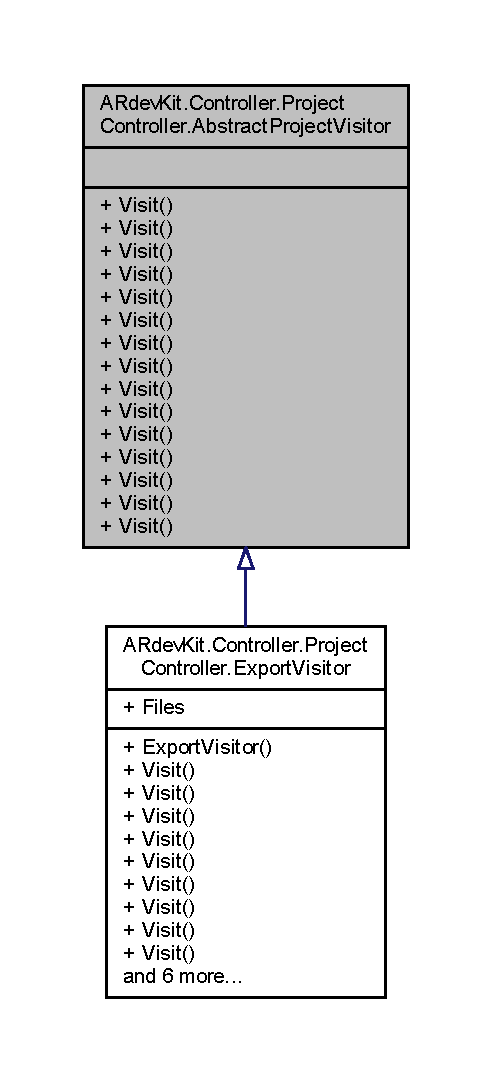
\includegraphics[width=236pt]{class_a_rdev_kit_1_1_controller_1_1_project_controller_1_1_abstract_project_visitor__inherit__graph}
\end{center}
\end{figure}


Collaboration diagram for A\-Rdev\-Kit.\-Controller.\-Project\-Controller.\-Abstract\-Project\-Visitor\-:
\nopagebreak
\begin{figure}[H]
\begin{center}
\leavevmode
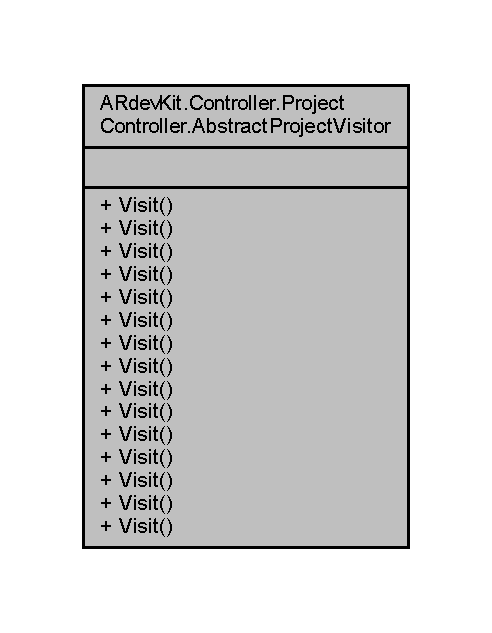
\includegraphics[width=236pt]{class_a_rdev_kit_1_1_controller_1_1_project_controller_1_1_abstract_project_visitor__coll__graph}
\end{center}
\end{figure}
\subsection*{Public Member Functions}
\begin{DoxyCompactItemize}
\item 
abstract void \hyperlink{class_a_rdev_kit_1_1_controller_1_1_project_controller_1_1_abstract_project_visitor_aafdd79d5f00d223cb7a5269344b55e8d}{Visit} (\hyperlink{class_a_rdev_kit_1_1_model_1_1_project_1_1_custom_user_event}{Custom\-User\-Event} cue)
\begin{DoxyCompactList}\small\item\em Visits the given Custom\-User\-Event. \end{DoxyCompactList}\item 
abstract void \hyperlink{class_a_rdev_kit_1_1_controller_1_1_project_controller_1_1_abstract_project_visitor_afc567731ac7e98ef86c2d26c5f22b4d8}{Visit} (\hyperlink{class_a_rdev_kit_1_1_model_1_1_project_1_1_chart}{Chart} chart)
\begin{DoxyCompactList}\small\item\em Visits the given Chart. \end{DoxyCompactList}\item 
abstract void \hyperlink{class_a_rdev_kit_1_1_controller_1_1_project_controller_1_1_abstract_project_visitor_a9f0a4ed7ac360a201255c1ed37759bee}{Visit} (\hyperlink{class_a_rdev_kit_1_1_model_1_1_project_1_1_image_augmentation}{Image\-Augmentation} image)
\begin{DoxyCompactList}\small\item\em Visits the given Image\-Augmentation. \end{DoxyCompactList}\item 
abstract void \hyperlink{class_a_rdev_kit_1_1_controller_1_1_project_controller_1_1_abstract_project_visitor_afd227a5cdb38cbfe2bb88ca22a5adf56}{Visit} (\hyperlink{class_a_rdev_kit_1_1_model_1_1_project_1_1_video_augmentation}{Video\-Augmentation} video)
\begin{DoxyCompactList}\small\item\em Visits the given Video\-Augmentation. \end{DoxyCompactList}\item 
abstract void \hyperlink{class_a_rdev_kit_1_1_controller_1_1_project_controller_1_1_abstract_project_visitor_ae89191e9e36e1de0ca8b2a68aa20c13f}{Visit} (\hyperlink{class_a_rdev_kit_1_1_model_1_1_project_1_1_db_source}{Db\-Source} source)
\begin{DoxyCompactList}\small\item\em Visits the given Db\-Source. \end{DoxyCompactList}\item 
abstract void \hyperlink{class_a_rdev_kit_1_1_controller_1_1_project_controller_1_1_abstract_project_visitor_a57f6cd714839140a46e4d68a29c65287}{Visit} (\hyperlink{class_a_rdev_kit_1_1_model_1_1_project_1_1_file_source}{File\-Source} source)
\begin{DoxyCompactList}\small\item\em Visits the given File\-Source. \end{DoxyCompactList}\item 
abstract void \hyperlink{class_a_rdev_kit_1_1_controller_1_1_project_controller_1_1_abstract_project_visitor_a81cd1e82508e62b748421a2e3f128fa2}{Visit} (\hyperlink{class_a_rdev_kit_1_1_model_1_1_project_1_1_markerless_fuser}{Markerless\-Fuser} markerless\-Fuser)
\begin{DoxyCompactList}\small\item\em Visits the given Markerless\-Fuser. \end{DoxyCompactList}\item 
abstract void \hyperlink{class_a_rdev_kit_1_1_controller_1_1_project_controller_1_1_abstract_project_visitor_a162cb32ccf792db44d5cb92604d1f799}{Visit} (\hyperlink{class_a_rdev_kit_1_1_model_1_1_project_1_1_marker_fuser}{Marker\-Fuser} marker\-Fuser)
\begin{DoxyCompactList}\small\item\em Visits the given Marker\-Fuser. \end{DoxyCompactList}\item 
abstract void \hyperlink{class_a_rdev_kit_1_1_controller_1_1_project_controller_1_1_abstract_project_visitor_ab954e7db5de1aafc57e082020eba3f3b}{Visit} (\hyperlink{class_a_rdev_kit_1_1_model_1_1_project_1_1_markerless_sensor}{Markerless\-Sensor} \hyperlink{class_a_rdev_kit_1_1_model_1_1_project_1_1_markerless_sensor}{Markerless\-Sensor})
\begin{DoxyCompactList}\small\item\em Visits the given Markerless\-Sensor. \end{DoxyCompactList}\item 
abstract void \hyperlink{class_a_rdev_kit_1_1_controller_1_1_project_controller_1_1_abstract_project_visitor_a70f8dcc9540bfd0a0d49ac4638898e7a}{Visit} (\hyperlink{class_a_rdev_kit_1_1_model_1_1_project_1_1_image_trackable}{Image\-Trackable} image)
\begin{DoxyCompactList}\small\item\em Visits the given Image\-Trackable. \end{DoxyCompactList}\item 
abstract void \hyperlink{class_a_rdev_kit_1_1_controller_1_1_project_controller_1_1_abstract_project_visitor_a2f87bcb8c5df6e3aeb5fca33d43e5fd8}{Visit} (\hyperlink{class_a_rdev_kit_1_1_model_1_1_project_1_1_picture_marker_sensor}{Picture\-Marker\-Sensor} picture\-Marker\-Sensor)
\begin{DoxyCompactList}\small\item\em Visits the given Picture\-Marker\-Sensor. \end{DoxyCompactList}\item 
abstract void \hyperlink{class_a_rdev_kit_1_1_controller_1_1_project_controller_1_1_abstract_project_visitor_a07ea2f0ff782d6d5c3c122575c2acc51}{Visit} (\hyperlink{class_a_rdev_kit_1_1_model_1_1_project_1_1_picture_marker}{Picture\-Marker} picture\-Marker)
\begin{DoxyCompactList}\small\item\em Visits the given Picture\-Marker. \end{DoxyCompactList}\item 
abstract void \hyperlink{class_a_rdev_kit_1_1_controller_1_1_project_controller_1_1_abstract_project_visitor_afce8054c78342330b871b0acc0bcdfad}{Visit} (\hyperlink{class_a_rdev_kit_1_1_model_1_1_project_1_1_marker_sensor}{Marker\-Sensor} id\-Marker\-Sensor)
\begin{DoxyCompactList}\small\item\em Visits the given Marker\-Sensor. \end{DoxyCompactList}\item 
abstract void \hyperlink{class_a_rdev_kit_1_1_controller_1_1_project_controller_1_1_abstract_project_visitor_a8f6463762a4fee7bab0e1bad63836abf}{Visit} (\hyperlink{class_a_rdev_kit_1_1_model_1_1_project_1_1_i_d_marker}{I\-D\-Marker} id\-Marker)
\begin{DoxyCompactList}\small\item\em Visits the given I\-D\-Marker. \end{DoxyCompactList}\item 
abstract void \hyperlink{class_a_rdev_kit_1_1_controller_1_1_project_controller_1_1_abstract_project_visitor_a6f3a8879b50f53e1d25fc87c588a59fa}{Visit} (\hyperlink{class_a_rdev_kit_1_1_model_1_1_project_1_1_project}{Project} project)
\begin{DoxyCompactList}\small\item\em Visits the given Project. \end{DoxyCompactList}\end{DoxyCompactItemize}


\subsection{Detailed Description}
An abstract project visitor. 

Imanuel, 17.\-01.\-2014. 

\subsection{Member Function Documentation}
\hypertarget{class_a_rdev_kit_1_1_controller_1_1_project_controller_1_1_abstract_project_visitor_aafdd79d5f00d223cb7a5269344b55e8d}{\index{A\-Rdev\-Kit\-::\-Controller\-::\-Project\-Controller\-::\-Abstract\-Project\-Visitor@{A\-Rdev\-Kit\-::\-Controller\-::\-Project\-Controller\-::\-Abstract\-Project\-Visitor}!Visit@{Visit}}
\index{Visit@{Visit}!ARdevKit::Controller::ProjectController::AbstractProjectVisitor@{A\-Rdev\-Kit\-::\-Controller\-::\-Project\-Controller\-::\-Abstract\-Project\-Visitor}}
\subsubsection[{Visit}]{\setlength{\rightskip}{0pt plus 5cm}abstract void A\-Rdev\-Kit.\-Controller.\-Project\-Controller.\-Abstract\-Project\-Visitor.\-Visit (
\begin{DoxyParamCaption}
\item[{{\bf Custom\-User\-Event}}]{cue}
\end{DoxyParamCaption}
)\hspace{0.3cm}{\ttfamily [pure virtual]}}}\label{class_a_rdev_kit_1_1_controller_1_1_project_controller_1_1_abstract_project_visitor_aafdd79d5f00d223cb7a5269344b55e8d}


Visits the given Custom\-User\-Event. 


\begin{DoxyParams}{Parameters}
{\em cue} & The custom user event. \\
\hline
\end{DoxyParams}


Implemented in \hyperlink{class_a_rdev_kit_1_1_controller_1_1_project_controller_1_1_export_visitor_a4d2802913e6ccb1a24e53c642d1b1cff}{A\-Rdev\-Kit.\-Controller.\-Project\-Controller.\-Export\-Visitor}.

\hypertarget{class_a_rdev_kit_1_1_controller_1_1_project_controller_1_1_abstract_project_visitor_afc567731ac7e98ef86c2d26c5f22b4d8}{\index{A\-Rdev\-Kit\-::\-Controller\-::\-Project\-Controller\-::\-Abstract\-Project\-Visitor@{A\-Rdev\-Kit\-::\-Controller\-::\-Project\-Controller\-::\-Abstract\-Project\-Visitor}!Visit@{Visit}}
\index{Visit@{Visit}!ARdevKit::Controller::ProjectController::AbstractProjectVisitor@{A\-Rdev\-Kit\-::\-Controller\-::\-Project\-Controller\-::\-Abstract\-Project\-Visitor}}
\subsubsection[{Visit}]{\setlength{\rightskip}{0pt plus 5cm}abstract void A\-Rdev\-Kit.\-Controller.\-Project\-Controller.\-Abstract\-Project\-Visitor.\-Visit (
\begin{DoxyParamCaption}
\item[{{\bf Chart}}]{chart}
\end{DoxyParamCaption}
)\hspace{0.3cm}{\ttfamily [pure virtual]}}}\label{class_a_rdev_kit_1_1_controller_1_1_project_controller_1_1_abstract_project_visitor_afc567731ac7e98ef86c2d26c5f22b4d8}


Visits the given Chart. 

Imanuel, 17.\-01.\-2014. 


\begin{DoxyParams}{Parameters}
{\em chart} & The chart. \\
\hline
\end{DoxyParams}


Implemented in \hyperlink{class_a_rdev_kit_1_1_controller_1_1_project_controller_1_1_export_visitor_a0e04a0743609a16eb7c872427755249e}{A\-Rdev\-Kit.\-Controller.\-Project\-Controller.\-Export\-Visitor}.

\hypertarget{class_a_rdev_kit_1_1_controller_1_1_project_controller_1_1_abstract_project_visitor_a9f0a4ed7ac360a201255c1ed37759bee}{\index{A\-Rdev\-Kit\-::\-Controller\-::\-Project\-Controller\-::\-Abstract\-Project\-Visitor@{A\-Rdev\-Kit\-::\-Controller\-::\-Project\-Controller\-::\-Abstract\-Project\-Visitor}!Visit@{Visit}}
\index{Visit@{Visit}!ARdevKit::Controller::ProjectController::AbstractProjectVisitor@{A\-Rdev\-Kit\-::\-Controller\-::\-Project\-Controller\-::\-Abstract\-Project\-Visitor}}
\subsubsection[{Visit}]{\setlength{\rightskip}{0pt plus 5cm}abstract void A\-Rdev\-Kit.\-Controller.\-Project\-Controller.\-Abstract\-Project\-Visitor.\-Visit (
\begin{DoxyParamCaption}
\item[{{\bf Image\-Augmentation}}]{image}
\end{DoxyParamCaption}
)\hspace{0.3cm}{\ttfamily [pure virtual]}}}\label{class_a_rdev_kit_1_1_controller_1_1_project_controller_1_1_abstract_project_visitor_a9f0a4ed7ac360a201255c1ed37759bee}


Visits the given Image\-Augmentation. 

Imanuel, 17.\-01.\-2014. 


\begin{DoxyParams}{Parameters}
{\em image} & The image. \\
\hline
\end{DoxyParams}


Implemented in \hyperlink{class_a_rdev_kit_1_1_controller_1_1_project_controller_1_1_export_visitor_a68256626e59d84b43153e95697ed1e3a}{A\-Rdev\-Kit.\-Controller.\-Project\-Controller.\-Export\-Visitor}.

\hypertarget{class_a_rdev_kit_1_1_controller_1_1_project_controller_1_1_abstract_project_visitor_afd227a5cdb38cbfe2bb88ca22a5adf56}{\index{A\-Rdev\-Kit\-::\-Controller\-::\-Project\-Controller\-::\-Abstract\-Project\-Visitor@{A\-Rdev\-Kit\-::\-Controller\-::\-Project\-Controller\-::\-Abstract\-Project\-Visitor}!Visit@{Visit}}
\index{Visit@{Visit}!ARdevKit::Controller::ProjectController::AbstractProjectVisitor@{A\-Rdev\-Kit\-::\-Controller\-::\-Project\-Controller\-::\-Abstract\-Project\-Visitor}}
\subsubsection[{Visit}]{\setlength{\rightskip}{0pt plus 5cm}abstract void A\-Rdev\-Kit.\-Controller.\-Project\-Controller.\-Abstract\-Project\-Visitor.\-Visit (
\begin{DoxyParamCaption}
\item[{{\bf Video\-Augmentation}}]{video}
\end{DoxyParamCaption}
)\hspace{0.3cm}{\ttfamily [pure virtual]}}}\label{class_a_rdev_kit_1_1_controller_1_1_project_controller_1_1_abstract_project_visitor_afd227a5cdb38cbfe2bb88ca22a5adf56}


Visits the given Video\-Augmentation. 

Imanuel, 29.\-01.\-2014. 


\begin{DoxyParams}{Parameters}
{\em video} & The video. \\
\hline
\end{DoxyParams}


Implemented in \hyperlink{class_a_rdev_kit_1_1_controller_1_1_project_controller_1_1_export_visitor_a190039e5dd86df278c99cfacedac3b63}{A\-Rdev\-Kit.\-Controller.\-Project\-Controller.\-Export\-Visitor}.

\hypertarget{class_a_rdev_kit_1_1_controller_1_1_project_controller_1_1_abstract_project_visitor_ae89191e9e36e1de0ca8b2a68aa20c13f}{\index{A\-Rdev\-Kit\-::\-Controller\-::\-Project\-Controller\-::\-Abstract\-Project\-Visitor@{A\-Rdev\-Kit\-::\-Controller\-::\-Project\-Controller\-::\-Abstract\-Project\-Visitor}!Visit@{Visit}}
\index{Visit@{Visit}!ARdevKit::Controller::ProjectController::AbstractProjectVisitor@{A\-Rdev\-Kit\-::\-Controller\-::\-Project\-Controller\-::\-Abstract\-Project\-Visitor}}
\subsubsection[{Visit}]{\setlength{\rightskip}{0pt plus 5cm}abstract void A\-Rdev\-Kit.\-Controller.\-Project\-Controller.\-Abstract\-Project\-Visitor.\-Visit (
\begin{DoxyParamCaption}
\item[{{\bf Db\-Source}}]{source}
\end{DoxyParamCaption}
)\hspace{0.3cm}{\ttfamily [pure virtual]}}}\label{class_a_rdev_kit_1_1_controller_1_1_project_controller_1_1_abstract_project_visitor_ae89191e9e36e1de0ca8b2a68aa20c13f}


Visits the given Db\-Source. 

Imanuel, 17.\-01.\-2014. 


\begin{DoxyParams}{Parameters}
{\em source} & Source for the. \\
\hline
\end{DoxyParams}


Implemented in \hyperlink{class_a_rdev_kit_1_1_controller_1_1_project_controller_1_1_export_visitor_a54481877bd367164a17916ff32f8da09}{A\-Rdev\-Kit.\-Controller.\-Project\-Controller.\-Export\-Visitor}.

\hypertarget{class_a_rdev_kit_1_1_controller_1_1_project_controller_1_1_abstract_project_visitor_a57f6cd714839140a46e4d68a29c65287}{\index{A\-Rdev\-Kit\-::\-Controller\-::\-Project\-Controller\-::\-Abstract\-Project\-Visitor@{A\-Rdev\-Kit\-::\-Controller\-::\-Project\-Controller\-::\-Abstract\-Project\-Visitor}!Visit@{Visit}}
\index{Visit@{Visit}!ARdevKit::Controller::ProjectController::AbstractProjectVisitor@{A\-Rdev\-Kit\-::\-Controller\-::\-Project\-Controller\-::\-Abstract\-Project\-Visitor}}
\subsubsection[{Visit}]{\setlength{\rightskip}{0pt plus 5cm}abstract void A\-Rdev\-Kit.\-Controller.\-Project\-Controller.\-Abstract\-Project\-Visitor.\-Visit (
\begin{DoxyParamCaption}
\item[{{\bf File\-Source}}]{source}
\end{DoxyParamCaption}
)\hspace{0.3cm}{\ttfamily [pure virtual]}}}\label{class_a_rdev_kit_1_1_controller_1_1_project_controller_1_1_abstract_project_visitor_a57f6cd714839140a46e4d68a29c65287}


Visits the given File\-Source. 

Imanuel, 23.\-01.\-2014. 


\begin{DoxyParams}{Parameters}
{\em source} & Source for the Abstract\-Dynamic2\-D\-Augmentation. \\
\hline
\end{DoxyParams}


Implemented in \hyperlink{class_a_rdev_kit_1_1_controller_1_1_project_controller_1_1_export_visitor_a078a2d0fef2fa5db4b6adcf4be50debe}{A\-Rdev\-Kit.\-Controller.\-Project\-Controller.\-Export\-Visitor}.

\hypertarget{class_a_rdev_kit_1_1_controller_1_1_project_controller_1_1_abstract_project_visitor_a81cd1e82508e62b748421a2e3f128fa2}{\index{A\-Rdev\-Kit\-::\-Controller\-::\-Project\-Controller\-::\-Abstract\-Project\-Visitor@{A\-Rdev\-Kit\-::\-Controller\-::\-Project\-Controller\-::\-Abstract\-Project\-Visitor}!Visit@{Visit}}
\index{Visit@{Visit}!ARdevKit::Controller::ProjectController::AbstractProjectVisitor@{A\-Rdev\-Kit\-::\-Controller\-::\-Project\-Controller\-::\-Abstract\-Project\-Visitor}}
\subsubsection[{Visit}]{\setlength{\rightskip}{0pt plus 5cm}abstract void A\-Rdev\-Kit.\-Controller.\-Project\-Controller.\-Abstract\-Project\-Visitor.\-Visit (
\begin{DoxyParamCaption}
\item[{{\bf Markerless\-Fuser}}]{markerless\-Fuser}
\end{DoxyParamCaption}
)\hspace{0.3cm}{\ttfamily [pure virtual]}}}\label{class_a_rdev_kit_1_1_controller_1_1_project_controller_1_1_abstract_project_visitor_a81cd1e82508e62b748421a2e3f128fa2}


Visits the given Markerless\-Fuser. 

Imanuel, 17.\-01.\-2014. 


\begin{DoxyParams}{Parameters}
{\em markerless\-Fuser} & The markerless fuser. \\
\hline
\end{DoxyParams}


Implemented in \hyperlink{class_a_rdev_kit_1_1_controller_1_1_project_controller_1_1_export_visitor_aae0293dd695393b0037fb62f0f5a1d28}{A\-Rdev\-Kit.\-Controller.\-Project\-Controller.\-Export\-Visitor}.

\hypertarget{class_a_rdev_kit_1_1_controller_1_1_project_controller_1_1_abstract_project_visitor_a162cb32ccf792db44d5cb92604d1f799}{\index{A\-Rdev\-Kit\-::\-Controller\-::\-Project\-Controller\-::\-Abstract\-Project\-Visitor@{A\-Rdev\-Kit\-::\-Controller\-::\-Project\-Controller\-::\-Abstract\-Project\-Visitor}!Visit@{Visit}}
\index{Visit@{Visit}!ARdevKit::Controller::ProjectController::AbstractProjectVisitor@{A\-Rdev\-Kit\-::\-Controller\-::\-Project\-Controller\-::\-Abstract\-Project\-Visitor}}
\subsubsection[{Visit}]{\setlength{\rightskip}{0pt plus 5cm}abstract void A\-Rdev\-Kit.\-Controller.\-Project\-Controller.\-Abstract\-Project\-Visitor.\-Visit (
\begin{DoxyParamCaption}
\item[{{\bf Marker\-Fuser}}]{marker\-Fuser}
\end{DoxyParamCaption}
)\hspace{0.3cm}{\ttfamily [pure virtual]}}}\label{class_a_rdev_kit_1_1_controller_1_1_project_controller_1_1_abstract_project_visitor_a162cb32ccf792db44d5cb92604d1f799}


Visits the given Marker\-Fuser. 

Imanuel, 17.\-01.\-2014. 


\begin{DoxyParams}{Parameters}
{\em marker\-Fuser} & The marker fuser. \\
\hline
\end{DoxyParams}


Implemented in \hyperlink{class_a_rdev_kit_1_1_controller_1_1_project_controller_1_1_export_visitor_a315b092cbd6a936b67d3ea690920bd95}{A\-Rdev\-Kit.\-Controller.\-Project\-Controller.\-Export\-Visitor}.

\hypertarget{class_a_rdev_kit_1_1_controller_1_1_project_controller_1_1_abstract_project_visitor_ab954e7db5de1aafc57e082020eba3f3b}{\index{A\-Rdev\-Kit\-::\-Controller\-::\-Project\-Controller\-::\-Abstract\-Project\-Visitor@{A\-Rdev\-Kit\-::\-Controller\-::\-Project\-Controller\-::\-Abstract\-Project\-Visitor}!Visit@{Visit}}
\index{Visit@{Visit}!ARdevKit::Controller::ProjectController::AbstractProjectVisitor@{A\-Rdev\-Kit\-::\-Controller\-::\-Project\-Controller\-::\-Abstract\-Project\-Visitor}}
\subsubsection[{Visit}]{\setlength{\rightskip}{0pt plus 5cm}abstract void A\-Rdev\-Kit.\-Controller.\-Project\-Controller.\-Abstract\-Project\-Visitor.\-Visit (
\begin{DoxyParamCaption}
\item[{{\bf Markerless\-Sensor}}]{Markerless\-Sensor}
\end{DoxyParamCaption}
)\hspace{0.3cm}{\ttfamily [pure virtual]}}}\label{class_a_rdev_kit_1_1_controller_1_1_project_controller_1_1_abstract_project_visitor_ab954e7db5de1aafc57e082020eba3f3b}


Visits the given Markerless\-Sensor. 

Imanuel, 17.\-01.\-2014. 


\begin{DoxyParams}{Parameters}
{\em Markerless\-Sensor} & The markerless sensor. \\
\hline
\end{DoxyParams}


Implemented in \hyperlink{class_a_rdev_kit_1_1_controller_1_1_project_controller_1_1_export_visitor_abf7c8bbff198ee8af664232c2fa394cb}{A\-Rdev\-Kit.\-Controller.\-Project\-Controller.\-Export\-Visitor}.

\hypertarget{class_a_rdev_kit_1_1_controller_1_1_project_controller_1_1_abstract_project_visitor_a70f8dcc9540bfd0a0d49ac4638898e7a}{\index{A\-Rdev\-Kit\-::\-Controller\-::\-Project\-Controller\-::\-Abstract\-Project\-Visitor@{A\-Rdev\-Kit\-::\-Controller\-::\-Project\-Controller\-::\-Abstract\-Project\-Visitor}!Visit@{Visit}}
\index{Visit@{Visit}!ARdevKit::Controller::ProjectController::AbstractProjectVisitor@{A\-Rdev\-Kit\-::\-Controller\-::\-Project\-Controller\-::\-Abstract\-Project\-Visitor}}
\subsubsection[{Visit}]{\setlength{\rightskip}{0pt plus 5cm}abstract void A\-Rdev\-Kit.\-Controller.\-Project\-Controller.\-Abstract\-Project\-Visitor.\-Visit (
\begin{DoxyParamCaption}
\item[{{\bf Image\-Trackable}}]{image}
\end{DoxyParamCaption}
)\hspace{0.3cm}{\ttfamily [pure virtual]}}}\label{class_a_rdev_kit_1_1_controller_1_1_project_controller_1_1_abstract_project_visitor_a70f8dcc9540bfd0a0d49ac4638898e7a}


Visits the given Image\-Trackable. 

Imanuel, 26.\-01.\-2014. 


\begin{DoxyParams}{Parameters}
{\em image} & The image. \\
\hline
\end{DoxyParams}


Implemented in \hyperlink{class_a_rdev_kit_1_1_controller_1_1_project_controller_1_1_export_visitor_a6ba67134957206067b97c6ebba5a9c8a}{A\-Rdev\-Kit.\-Controller.\-Project\-Controller.\-Export\-Visitor}.

\hypertarget{class_a_rdev_kit_1_1_controller_1_1_project_controller_1_1_abstract_project_visitor_a2f87bcb8c5df6e3aeb5fca33d43e5fd8}{\index{A\-Rdev\-Kit\-::\-Controller\-::\-Project\-Controller\-::\-Abstract\-Project\-Visitor@{A\-Rdev\-Kit\-::\-Controller\-::\-Project\-Controller\-::\-Abstract\-Project\-Visitor}!Visit@{Visit}}
\index{Visit@{Visit}!ARdevKit::Controller::ProjectController::AbstractProjectVisitor@{A\-Rdev\-Kit\-::\-Controller\-::\-Project\-Controller\-::\-Abstract\-Project\-Visitor}}
\subsubsection[{Visit}]{\setlength{\rightskip}{0pt plus 5cm}abstract void A\-Rdev\-Kit.\-Controller.\-Project\-Controller.\-Abstract\-Project\-Visitor.\-Visit (
\begin{DoxyParamCaption}
\item[{{\bf Picture\-Marker\-Sensor}}]{picture\-Marker\-Sensor}
\end{DoxyParamCaption}
)\hspace{0.3cm}{\ttfamily [pure virtual]}}}\label{class_a_rdev_kit_1_1_controller_1_1_project_controller_1_1_abstract_project_visitor_a2f87bcb8c5df6e3aeb5fca33d43e5fd8}


Visits the given Picture\-Marker\-Sensor. 

Imanuel, 17.\-01.\-2014. 


\begin{DoxyParams}{Parameters}
{\em picture\-Marker\-Sensor} & The picture marker sensor. \\
\hline
\end{DoxyParams}


Implemented in \hyperlink{class_a_rdev_kit_1_1_controller_1_1_project_controller_1_1_export_visitor_a567d0ff197539453cc2c34b11f12ad59}{A\-Rdev\-Kit.\-Controller.\-Project\-Controller.\-Export\-Visitor}.

\hypertarget{class_a_rdev_kit_1_1_controller_1_1_project_controller_1_1_abstract_project_visitor_a07ea2f0ff782d6d5c3c122575c2acc51}{\index{A\-Rdev\-Kit\-::\-Controller\-::\-Project\-Controller\-::\-Abstract\-Project\-Visitor@{A\-Rdev\-Kit\-::\-Controller\-::\-Project\-Controller\-::\-Abstract\-Project\-Visitor}!Visit@{Visit}}
\index{Visit@{Visit}!ARdevKit::Controller::ProjectController::AbstractProjectVisitor@{A\-Rdev\-Kit\-::\-Controller\-::\-Project\-Controller\-::\-Abstract\-Project\-Visitor}}
\subsubsection[{Visit}]{\setlength{\rightskip}{0pt plus 5cm}abstract void A\-Rdev\-Kit.\-Controller.\-Project\-Controller.\-Abstract\-Project\-Visitor.\-Visit (
\begin{DoxyParamCaption}
\item[{{\bf Picture\-Marker}}]{picture\-Marker}
\end{DoxyParamCaption}
)\hspace{0.3cm}{\ttfamily [pure virtual]}}}\label{class_a_rdev_kit_1_1_controller_1_1_project_controller_1_1_abstract_project_visitor_a07ea2f0ff782d6d5c3c122575c2acc51}


Visits the given Picture\-Marker. 

Imanuel, 17.\-01.\-2014. 


\begin{DoxyParams}{Parameters}
{\em picture\-Marker} & The picture marker. \\
\hline
\end{DoxyParams}


Implemented in \hyperlink{class_a_rdev_kit_1_1_controller_1_1_project_controller_1_1_export_visitor_a384b6fc84602fd29bedff296b083b3a0}{A\-Rdev\-Kit.\-Controller.\-Project\-Controller.\-Export\-Visitor}.

\hypertarget{class_a_rdev_kit_1_1_controller_1_1_project_controller_1_1_abstract_project_visitor_afce8054c78342330b871b0acc0bcdfad}{\index{A\-Rdev\-Kit\-::\-Controller\-::\-Project\-Controller\-::\-Abstract\-Project\-Visitor@{A\-Rdev\-Kit\-::\-Controller\-::\-Project\-Controller\-::\-Abstract\-Project\-Visitor}!Visit@{Visit}}
\index{Visit@{Visit}!ARdevKit::Controller::ProjectController::AbstractProjectVisitor@{A\-Rdev\-Kit\-::\-Controller\-::\-Project\-Controller\-::\-Abstract\-Project\-Visitor}}
\subsubsection[{Visit}]{\setlength{\rightskip}{0pt plus 5cm}abstract void A\-Rdev\-Kit.\-Controller.\-Project\-Controller.\-Abstract\-Project\-Visitor.\-Visit (
\begin{DoxyParamCaption}
\item[{{\bf Marker\-Sensor}}]{id\-Marker\-Sensor}
\end{DoxyParamCaption}
)\hspace{0.3cm}{\ttfamily [pure virtual]}}}\label{class_a_rdev_kit_1_1_controller_1_1_project_controller_1_1_abstract_project_visitor_afce8054c78342330b871b0acc0bcdfad}


Visits the given Marker\-Sensor. 

Imanuel, 17.\-01.\-2014. 


\begin{DoxyParams}{Parameters}
{\em id\-Marker\-Sensor} & The identifier marker sensor. \\
\hline
\end{DoxyParams}


Implemented in \hyperlink{class_a_rdev_kit_1_1_controller_1_1_project_controller_1_1_export_visitor_a0e82718aa35b9bff19cd6db0b33f3d5c}{A\-Rdev\-Kit.\-Controller.\-Project\-Controller.\-Export\-Visitor}.

\hypertarget{class_a_rdev_kit_1_1_controller_1_1_project_controller_1_1_abstract_project_visitor_a8f6463762a4fee7bab0e1bad63836abf}{\index{A\-Rdev\-Kit\-::\-Controller\-::\-Project\-Controller\-::\-Abstract\-Project\-Visitor@{A\-Rdev\-Kit\-::\-Controller\-::\-Project\-Controller\-::\-Abstract\-Project\-Visitor}!Visit@{Visit}}
\index{Visit@{Visit}!ARdevKit::Controller::ProjectController::AbstractProjectVisitor@{A\-Rdev\-Kit\-::\-Controller\-::\-Project\-Controller\-::\-Abstract\-Project\-Visitor}}
\subsubsection[{Visit}]{\setlength{\rightskip}{0pt plus 5cm}abstract void A\-Rdev\-Kit.\-Controller.\-Project\-Controller.\-Abstract\-Project\-Visitor.\-Visit (
\begin{DoxyParamCaption}
\item[{{\bf I\-D\-Marker}}]{id\-Marker}
\end{DoxyParamCaption}
)\hspace{0.3cm}{\ttfamily [pure virtual]}}}\label{class_a_rdev_kit_1_1_controller_1_1_project_controller_1_1_abstract_project_visitor_a8f6463762a4fee7bab0e1bad63836abf}


Visits the given I\-D\-Marker. 

Imanuel, 17.\-01.\-2014. 


\begin{DoxyParams}{Parameters}
{\em id\-Marker} & The identifier marker. \\
\hline
\end{DoxyParams}


Implemented in \hyperlink{class_a_rdev_kit_1_1_controller_1_1_project_controller_1_1_export_visitor_aa4ad67b0cb408d8ec6aaf48906f1e5b3}{A\-Rdev\-Kit.\-Controller.\-Project\-Controller.\-Export\-Visitor}.

\hypertarget{class_a_rdev_kit_1_1_controller_1_1_project_controller_1_1_abstract_project_visitor_a6f3a8879b50f53e1d25fc87c588a59fa}{\index{A\-Rdev\-Kit\-::\-Controller\-::\-Project\-Controller\-::\-Abstract\-Project\-Visitor@{A\-Rdev\-Kit\-::\-Controller\-::\-Project\-Controller\-::\-Abstract\-Project\-Visitor}!Visit@{Visit}}
\index{Visit@{Visit}!ARdevKit::Controller::ProjectController::AbstractProjectVisitor@{A\-Rdev\-Kit\-::\-Controller\-::\-Project\-Controller\-::\-Abstract\-Project\-Visitor}}
\subsubsection[{Visit}]{\setlength{\rightskip}{0pt plus 5cm}abstract void A\-Rdev\-Kit.\-Controller.\-Project\-Controller.\-Abstract\-Project\-Visitor.\-Visit (
\begin{DoxyParamCaption}
\item[{{\bf Project}}]{project}
\end{DoxyParamCaption}
)\hspace{0.3cm}{\ttfamily [pure virtual]}}}\label{class_a_rdev_kit_1_1_controller_1_1_project_controller_1_1_abstract_project_visitor_a6f3a8879b50f53e1d25fc87c588a59fa}


Visits the given Project. 

Imanuel, 17.\-01.\-2014. 


\begin{DoxyParams}{Parameters}
{\em project} & The project. \\
\hline
\end{DoxyParams}


Implemented in \hyperlink{class_a_rdev_kit_1_1_controller_1_1_project_controller_1_1_export_visitor_ad58774c6778421b6bf85a6c70029a3d9}{A\-Rdev\-Kit.\-Controller.\-Project\-Controller.\-Export\-Visitor}.


\hypertarget{class_a_rdev_kit_1_1_model_1_1_project_1_1_abstract_sensor}{\section{A\-Rdev\-Kit.\-Model.\-Project.\-Abstract\-Sensor Class Reference}
\label{class_a_rdev_kit_1_1_model_1_1_project_1_1_abstract_sensor}\index{A\-Rdev\-Kit.\-Model.\-Project.\-Abstract\-Sensor@{A\-Rdev\-Kit.\-Model.\-Project.\-Abstract\-Sensor}}
}


An \hyperlink{class_a_rdev_kit_1_1_model_1_1_project_1_1_abstract_sensor}{Abstract\-Sensor} has a name, a \hyperlink{class_a_rdev_kit_1_1_model_1_1_project_1_1_abstract_sensor_a01251db96ea5e0fb0abe1df0a129e751}{sensor\-Type}, and can have a \hyperlink{class_a_rdev_kit_1_1_model_1_1_project_1_1_abstract_sensor_a29b9e916f374e31196689e9d7ac73123}{sensor\-Sub\-Type}. Moreover it has a \hyperlink{class_a_rdev_kit_1_1_model_1_1_project_1_1_abstract_sensor_a2f9524a6aba4331373c0c1968b2f6f4d}{sensor\-I\-D\-Base} which is used to create the \hyperlink{class_a_rdev_kit_1_1_model_1_1_project_1_1_abstract_sensor_ae12a6c3bfe5686d888d7e36c9b19df47}{sensor\-I\-D\-String}.  




Inheritance diagram for A\-Rdev\-Kit.\-Model.\-Project.\-Abstract\-Sensor\-:
\nopagebreak
\begin{figure}[H]
\begin{center}
\leavevmode
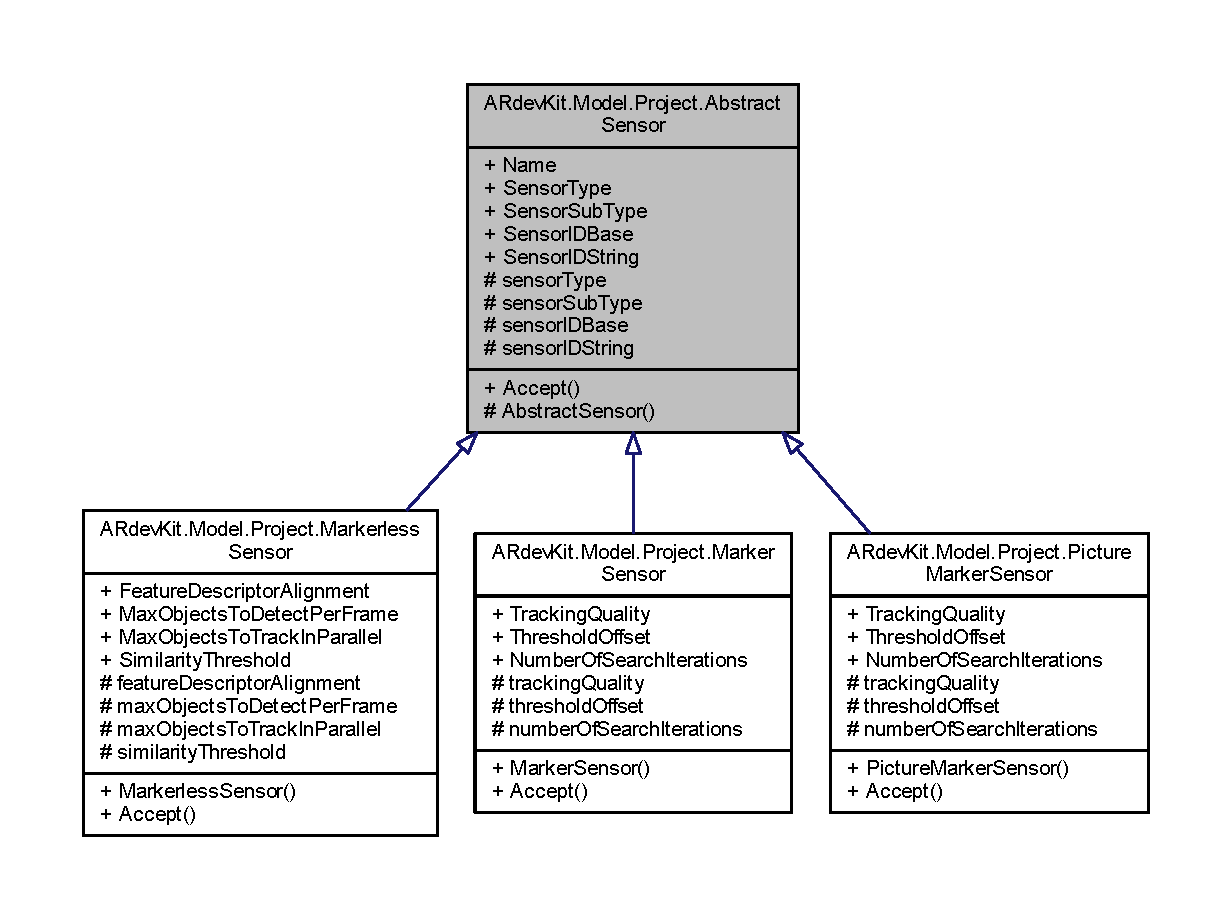
\includegraphics[width=350pt]{class_a_rdev_kit_1_1_model_1_1_project_1_1_abstract_sensor__inherit__graph}
\end{center}
\end{figure}


Collaboration diagram for A\-Rdev\-Kit.\-Model.\-Project.\-Abstract\-Sensor\-:
\nopagebreak
\begin{figure}[H]
\begin{center}
\leavevmode
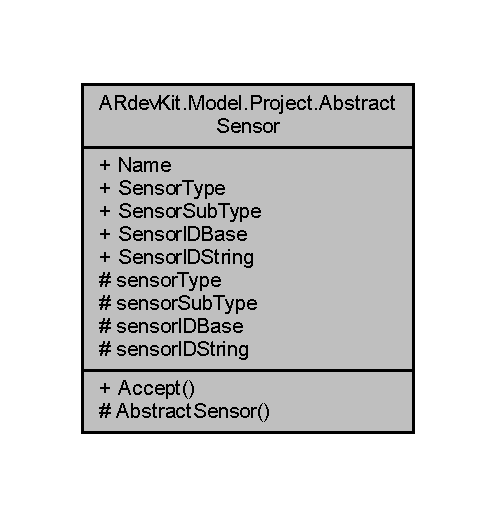
\includegraphics[width=238pt]{class_a_rdev_kit_1_1_model_1_1_project_1_1_abstract_sensor__coll__graph}
\end{center}
\end{figure}
\subsection*{Public Types}
\begin{DoxyCompactItemize}
\item 
enum \hyperlink{class_a_rdev_kit_1_1_model_1_1_project_1_1_abstract_sensor_a1954adedcf2a2f61256c9b11fe0c8386}{Sensor\-Types} \{ {\bfseries Feature\-Based\-Sensor\-Source}, 
{\bfseries Marker\-Based\-Sensor\-Source}
 \}
\begin{DoxyCompactList}\small\item\em Flags for specifying Sensor\-Types. \end{DoxyCompactList}\item 
enum \hyperlink{class_a_rdev_kit_1_1_model_1_1_project_1_1_abstract_sensor_af7b41fc81d926ed779ca02ef894fcddf}{Sensor\-Sub\-Types} \{ {\bfseries None}, 
{\bfseries Fast}, 
{\bfseries Robust}
 \}
\begin{DoxyCompactList}\small\item\em Flags for specifying Sensor\-Sub\-Types. \end{DoxyCompactList}\item 
enum \hyperlink{class_a_rdev_kit_1_1_model_1_1_project_1_1_abstract_sensor_a8eecc60106e6a54a3e096c63a7d4d012}{Sensor\-I\-D\-Bases} \{ {\bfseries Feature\-Tracking}, 
{\bfseries Marker\-Tracking}
 \}
\begin{DoxyCompactList}\small\item\em Flags for specifying Sensor\-I\-D\-Bases. \end{DoxyCompactList}\end{DoxyCompactItemize}
\subsection*{Public Member Functions}
\begin{DoxyCompactItemize}
\item 
abstract void \hyperlink{class_a_rdev_kit_1_1_model_1_1_project_1_1_abstract_sensor_a4ff825b76bdd9f01a93ca670d02c219c}{Accept} (\hyperlink{class_a_rdev_kit_1_1_controller_1_1_project_controller_1_1_abstract_project_visitor}{Abstract\-Project\-Visitor} visitor)
\begin{DoxyCompactList}\small\item\em Accepts the given visitor. \end{DoxyCompactList}\end{DoxyCompactItemize}
\subsection*{Protected Member Functions}
\begin{DoxyCompactItemize}
\item 
\hyperlink{class_a_rdev_kit_1_1_model_1_1_project_1_1_abstract_sensor_ac267c5a8c7792a6c0ba07108102c0706}{Abstract\-Sensor} ()
\begin{DoxyCompactList}\small\item\em Initializes no new instance of the \hyperlink{class_a_rdev_kit_1_1_model_1_1_project_1_1_abstract_sensor}{Abstract\-Sensor} class, but can be used in inheriting classes. \end{DoxyCompactList}\end{DoxyCompactItemize}
\subsection*{Protected Attributes}
\begin{DoxyCompactItemize}
\item 
\hyperlink{class_a_rdev_kit_1_1_model_1_1_project_1_1_abstract_sensor_a1954adedcf2a2f61256c9b11fe0c8386}{Sensor\-Types} \hyperlink{class_a_rdev_kit_1_1_model_1_1_project_1_1_abstract_sensor_a01251db96ea5e0fb0abe1df0a129e751}{sensor\-Type}
\begin{DoxyCompactList}\small\item\em Type of the sensor. \end{DoxyCompactList}\item 
\hyperlink{class_a_rdev_kit_1_1_model_1_1_project_1_1_abstract_sensor_af7b41fc81d926ed779ca02ef894fcddf}{Sensor\-Sub\-Types} \hyperlink{class_a_rdev_kit_1_1_model_1_1_project_1_1_abstract_sensor_a29b9e916f374e31196689e9d7ac73123}{sensor\-Sub\-Type}
\begin{DoxyCompactList}\small\item\em Sub\-Type of the sensor. \end{DoxyCompactList}\item 
\hyperlink{class_a_rdev_kit_1_1_model_1_1_project_1_1_abstract_sensor_a8eecc60106e6a54a3e096c63a7d4d012}{Sensor\-I\-D\-Bases} \hyperlink{class_a_rdev_kit_1_1_model_1_1_project_1_1_abstract_sensor_a2f9524a6aba4331373c0c1968b2f6f4d}{sensor\-I\-D\-Base}
\begin{DoxyCompactList}\small\item\em The sensor identifier base. \end{DoxyCompactList}\item 
string \hyperlink{class_a_rdev_kit_1_1_model_1_1_project_1_1_abstract_sensor_ae12a6c3bfe5686d888d7e36c9b19df47}{sensor\-I\-D\-String}
\begin{DoxyCompactList}\small\item\em The sensor identifier string. \end{DoxyCompactList}\end{DoxyCompactItemize}
\subsection*{Properties}
\begin{DoxyCompactItemize}
\item 
string \hyperlink{class_a_rdev_kit_1_1_model_1_1_project_1_1_abstract_sensor_ae9ff3a8ab9d8d8a357173cfa55a7030f}{Name}\hspace{0.3cm}{\ttfamily  \mbox{[}get, set\mbox{]}}
\begin{DoxyCompactList}\small\item\em Gets or sets the name. \end{DoxyCompactList}\item 
\hyperlink{class_a_rdev_kit_1_1_model_1_1_project_1_1_abstract_sensor_a1954adedcf2a2f61256c9b11fe0c8386}{Sensor\-Types} \hyperlink{class_a_rdev_kit_1_1_model_1_1_project_1_1_abstract_sensor_a66bde8348688b03400befc56c6ce8384}{Sensor\-Type}\hspace{0.3cm}{\ttfamily  \mbox{[}get, set\mbox{]}}
\begin{DoxyCompactList}\small\item\em Gets or sets the type of the sensor. \end{DoxyCompactList}\item 
\hyperlink{class_a_rdev_kit_1_1_model_1_1_project_1_1_abstract_sensor_af7b41fc81d926ed779ca02ef894fcddf}{Sensor\-Sub\-Types} \hyperlink{class_a_rdev_kit_1_1_model_1_1_project_1_1_abstract_sensor_a092d1bd99165833488f9ce744a1bf65d}{Sensor\-Sub\-Type}\hspace{0.3cm}{\ttfamily  \mbox{[}get, set\mbox{]}}
\begin{DoxyCompactList}\small\item\em Gets or sets the Sub\-Type of the sensor. \end{DoxyCompactList}\item 
\hyperlink{class_a_rdev_kit_1_1_model_1_1_project_1_1_abstract_sensor_a8eecc60106e6a54a3e096c63a7d4d012}{Sensor\-I\-D\-Bases} \hyperlink{class_a_rdev_kit_1_1_model_1_1_project_1_1_abstract_sensor_a51a87ecf568c53df079db7af4a553bc6}{Sensor\-I\-D\-Base}\hspace{0.3cm}{\ttfamily  \mbox{[}get, set\mbox{]}}
\begin{DoxyCompactList}\small\item\em Gets or sets the sensor identifier base. \end{DoxyCompactList}\item 
string \hyperlink{class_a_rdev_kit_1_1_model_1_1_project_1_1_abstract_sensor_a054724aa9c411a5f813d977c7c1f620c}{Sensor\-I\-D\-String}\hspace{0.3cm}{\ttfamily  \mbox{[}get, set\mbox{]}}
\begin{DoxyCompactList}\small\item\em Gets or sets the sensor identifier string. \end{DoxyCompactList}\end{DoxyCompactItemize}


\subsection{Detailed Description}
An \hyperlink{class_a_rdev_kit_1_1_model_1_1_project_1_1_abstract_sensor}{Abstract\-Sensor} has a name, a \hyperlink{class_a_rdev_kit_1_1_model_1_1_project_1_1_abstract_sensor_a01251db96ea5e0fb0abe1df0a129e751}{sensor\-Type}, and can have a \hyperlink{class_a_rdev_kit_1_1_model_1_1_project_1_1_abstract_sensor_a29b9e916f374e31196689e9d7ac73123}{sensor\-Sub\-Type}. Moreover it has a \hyperlink{class_a_rdev_kit_1_1_model_1_1_project_1_1_abstract_sensor_a2f9524a6aba4331373c0c1968b2f6f4d}{sensor\-I\-D\-Base} which is used to create the \hyperlink{class_a_rdev_kit_1_1_model_1_1_project_1_1_abstract_sensor_ae12a6c3bfe5686d888d7e36c9b19df47}{sensor\-I\-D\-String}. 

Imanuel, 17.\-01.\-2014. 

\subsection{Member Enumeration Documentation}
\hypertarget{class_a_rdev_kit_1_1_model_1_1_project_1_1_abstract_sensor_a8eecc60106e6a54a3e096c63a7d4d012}{\index{A\-Rdev\-Kit\-::\-Model\-::\-Project\-::\-Abstract\-Sensor@{A\-Rdev\-Kit\-::\-Model\-::\-Project\-::\-Abstract\-Sensor}!Sensor\-I\-D\-Bases@{Sensor\-I\-D\-Bases}}
\index{Sensor\-I\-D\-Bases@{Sensor\-I\-D\-Bases}!ARdevKit::Model::Project::AbstractSensor@{A\-Rdev\-Kit\-::\-Model\-::\-Project\-::\-Abstract\-Sensor}}
\subsubsection[{Sensor\-I\-D\-Bases}]{\setlength{\rightskip}{0pt plus 5cm}enum {\bf A\-Rdev\-Kit.\-Model.\-Project.\-Abstract\-Sensor.\-Sensor\-I\-D\-Bases}}}\label{class_a_rdev_kit_1_1_model_1_1_project_1_1_abstract_sensor_a8eecc60106e6a54a3e096c63a7d4d012}


Flags for specifying Sensor\-I\-D\-Bases. 

Imanuel, 17.\-01.\-2014. \hypertarget{class_a_rdev_kit_1_1_model_1_1_project_1_1_abstract_sensor_af7b41fc81d926ed779ca02ef894fcddf}{\index{A\-Rdev\-Kit\-::\-Model\-::\-Project\-::\-Abstract\-Sensor@{A\-Rdev\-Kit\-::\-Model\-::\-Project\-::\-Abstract\-Sensor}!Sensor\-Sub\-Types@{Sensor\-Sub\-Types}}
\index{Sensor\-Sub\-Types@{Sensor\-Sub\-Types}!ARdevKit::Model::Project::AbstractSensor@{A\-Rdev\-Kit\-::\-Model\-::\-Project\-::\-Abstract\-Sensor}}
\subsubsection[{Sensor\-Sub\-Types}]{\setlength{\rightskip}{0pt plus 5cm}enum {\bf A\-Rdev\-Kit.\-Model.\-Project.\-Abstract\-Sensor.\-Sensor\-Sub\-Types}}}\label{class_a_rdev_kit_1_1_model_1_1_project_1_1_abstract_sensor_af7b41fc81d926ed779ca02ef894fcddf}


Flags for specifying Sensor\-Sub\-Types. 

Imanuel, 17.\-01.\-2014. \hypertarget{class_a_rdev_kit_1_1_model_1_1_project_1_1_abstract_sensor_a1954adedcf2a2f61256c9b11fe0c8386}{\index{A\-Rdev\-Kit\-::\-Model\-::\-Project\-::\-Abstract\-Sensor@{A\-Rdev\-Kit\-::\-Model\-::\-Project\-::\-Abstract\-Sensor}!Sensor\-Types@{Sensor\-Types}}
\index{Sensor\-Types@{Sensor\-Types}!ARdevKit::Model::Project::AbstractSensor@{A\-Rdev\-Kit\-::\-Model\-::\-Project\-::\-Abstract\-Sensor}}
\subsubsection[{Sensor\-Types}]{\setlength{\rightskip}{0pt plus 5cm}enum {\bf A\-Rdev\-Kit.\-Model.\-Project.\-Abstract\-Sensor.\-Sensor\-Types}}}\label{class_a_rdev_kit_1_1_model_1_1_project_1_1_abstract_sensor_a1954adedcf2a2f61256c9b11fe0c8386}


Flags for specifying Sensor\-Types. 

Imanuel, 17.\-01.\-2014. 

\subsection{Constructor \& Destructor Documentation}
\hypertarget{class_a_rdev_kit_1_1_model_1_1_project_1_1_abstract_sensor_ac267c5a8c7792a6c0ba07108102c0706}{\index{A\-Rdev\-Kit\-::\-Model\-::\-Project\-::\-Abstract\-Sensor@{A\-Rdev\-Kit\-::\-Model\-::\-Project\-::\-Abstract\-Sensor}!Abstract\-Sensor@{Abstract\-Sensor}}
\index{Abstract\-Sensor@{Abstract\-Sensor}!ARdevKit::Model::Project::AbstractSensor@{A\-Rdev\-Kit\-::\-Model\-::\-Project\-::\-Abstract\-Sensor}}
\subsubsection[{Abstract\-Sensor}]{\setlength{\rightskip}{0pt plus 5cm}A\-Rdev\-Kit.\-Model.\-Project.\-Abstract\-Sensor.\-Abstract\-Sensor (
\begin{DoxyParamCaption}
{}
\end{DoxyParamCaption}
)\hspace{0.3cm}{\ttfamily [protected]}}}\label{class_a_rdev_kit_1_1_model_1_1_project_1_1_abstract_sensor_ac267c5a8c7792a6c0ba07108102c0706}


Initializes no new instance of the \hyperlink{class_a_rdev_kit_1_1_model_1_1_project_1_1_abstract_sensor}{Abstract\-Sensor} class, but can be used in inheriting classes. 



\subsection{Member Function Documentation}
\hypertarget{class_a_rdev_kit_1_1_model_1_1_project_1_1_abstract_sensor_a4ff825b76bdd9f01a93ca670d02c219c}{\index{A\-Rdev\-Kit\-::\-Model\-::\-Project\-::\-Abstract\-Sensor@{A\-Rdev\-Kit\-::\-Model\-::\-Project\-::\-Abstract\-Sensor}!Accept@{Accept}}
\index{Accept@{Accept}!ARdevKit::Model::Project::AbstractSensor@{A\-Rdev\-Kit\-::\-Model\-::\-Project\-::\-Abstract\-Sensor}}
\subsubsection[{Accept}]{\setlength{\rightskip}{0pt plus 5cm}abstract void A\-Rdev\-Kit.\-Model.\-Project.\-Abstract\-Sensor.\-Accept (
\begin{DoxyParamCaption}
\item[{{\bf Abstract\-Project\-Visitor}}]{visitor}
\end{DoxyParamCaption}
)\hspace{0.3cm}{\ttfamily [pure virtual]}}}\label{class_a_rdev_kit_1_1_model_1_1_project_1_1_abstract_sensor_a4ff825b76bdd9f01a93ca670d02c219c}


Accepts the given visitor. 


\begin{DoxyParams}{Parameters}
{\em visitor} & The visitor.\\
\hline
\end{DoxyParams}


Imanuel, 17.\-01.\-2014. 

Implemented in \hyperlink{class_a_rdev_kit_1_1_model_1_1_project_1_1_markerless_sensor_a28dd4f8d16e0112ae1f1bfd948c90c59}{A\-Rdev\-Kit.\-Model.\-Project.\-Markerless\-Sensor}, \hyperlink{class_a_rdev_kit_1_1_model_1_1_project_1_1_picture_marker_sensor_a4c36ac6cf5bd103a418b5ae21492b70a}{A\-Rdev\-Kit.\-Model.\-Project.\-Picture\-Marker\-Sensor}, and \hyperlink{class_a_rdev_kit_1_1_model_1_1_project_1_1_marker_sensor_a21f889bd4916cb1ee7f455a9f644b72a}{A\-Rdev\-Kit.\-Model.\-Project.\-Marker\-Sensor}.



\subsection{Member Data Documentation}
\hypertarget{class_a_rdev_kit_1_1_model_1_1_project_1_1_abstract_sensor_a2f9524a6aba4331373c0c1968b2f6f4d}{\index{A\-Rdev\-Kit\-::\-Model\-::\-Project\-::\-Abstract\-Sensor@{A\-Rdev\-Kit\-::\-Model\-::\-Project\-::\-Abstract\-Sensor}!sensor\-I\-D\-Base@{sensor\-I\-D\-Base}}
\index{sensor\-I\-D\-Base@{sensor\-I\-D\-Base}!ARdevKit::Model::Project::AbstractSensor@{A\-Rdev\-Kit\-::\-Model\-::\-Project\-::\-Abstract\-Sensor}}
\subsubsection[{sensor\-I\-D\-Base}]{\setlength{\rightskip}{0pt plus 5cm}{\bf Sensor\-I\-D\-Bases} A\-Rdev\-Kit.\-Model.\-Project.\-Abstract\-Sensor.\-sensor\-I\-D\-Base\hspace{0.3cm}{\ttfamily [protected]}}}\label{class_a_rdev_kit_1_1_model_1_1_project_1_1_abstract_sensor_a2f9524a6aba4331373c0c1968b2f6f4d}


The sensor identifier base. 

\hypertarget{class_a_rdev_kit_1_1_model_1_1_project_1_1_abstract_sensor_ae12a6c3bfe5686d888d7e36c9b19df47}{\index{A\-Rdev\-Kit\-::\-Model\-::\-Project\-::\-Abstract\-Sensor@{A\-Rdev\-Kit\-::\-Model\-::\-Project\-::\-Abstract\-Sensor}!sensor\-I\-D\-String@{sensor\-I\-D\-String}}
\index{sensor\-I\-D\-String@{sensor\-I\-D\-String}!ARdevKit::Model::Project::AbstractSensor@{A\-Rdev\-Kit\-::\-Model\-::\-Project\-::\-Abstract\-Sensor}}
\subsubsection[{sensor\-I\-D\-String}]{\setlength{\rightskip}{0pt plus 5cm}string A\-Rdev\-Kit.\-Model.\-Project.\-Abstract\-Sensor.\-sensor\-I\-D\-String\hspace{0.3cm}{\ttfamily [protected]}}}\label{class_a_rdev_kit_1_1_model_1_1_project_1_1_abstract_sensor_ae12a6c3bfe5686d888d7e36c9b19df47}


The sensor identifier string. 

\hypertarget{class_a_rdev_kit_1_1_model_1_1_project_1_1_abstract_sensor_a29b9e916f374e31196689e9d7ac73123}{\index{A\-Rdev\-Kit\-::\-Model\-::\-Project\-::\-Abstract\-Sensor@{A\-Rdev\-Kit\-::\-Model\-::\-Project\-::\-Abstract\-Sensor}!sensor\-Sub\-Type@{sensor\-Sub\-Type}}
\index{sensor\-Sub\-Type@{sensor\-Sub\-Type}!ARdevKit::Model::Project::AbstractSensor@{A\-Rdev\-Kit\-::\-Model\-::\-Project\-::\-Abstract\-Sensor}}
\subsubsection[{sensor\-Sub\-Type}]{\setlength{\rightskip}{0pt plus 5cm}{\bf Sensor\-Sub\-Types} A\-Rdev\-Kit.\-Model.\-Project.\-Abstract\-Sensor.\-sensor\-Sub\-Type\hspace{0.3cm}{\ttfamily [protected]}}}\label{class_a_rdev_kit_1_1_model_1_1_project_1_1_abstract_sensor_a29b9e916f374e31196689e9d7ac73123}


Sub\-Type of the sensor. 

\hypertarget{class_a_rdev_kit_1_1_model_1_1_project_1_1_abstract_sensor_a01251db96ea5e0fb0abe1df0a129e751}{\index{A\-Rdev\-Kit\-::\-Model\-::\-Project\-::\-Abstract\-Sensor@{A\-Rdev\-Kit\-::\-Model\-::\-Project\-::\-Abstract\-Sensor}!sensor\-Type@{sensor\-Type}}
\index{sensor\-Type@{sensor\-Type}!ARdevKit::Model::Project::AbstractSensor@{A\-Rdev\-Kit\-::\-Model\-::\-Project\-::\-Abstract\-Sensor}}
\subsubsection[{sensor\-Type}]{\setlength{\rightskip}{0pt plus 5cm}{\bf Sensor\-Types} A\-Rdev\-Kit.\-Model.\-Project.\-Abstract\-Sensor.\-sensor\-Type\hspace{0.3cm}{\ttfamily [protected]}}}\label{class_a_rdev_kit_1_1_model_1_1_project_1_1_abstract_sensor_a01251db96ea5e0fb0abe1df0a129e751}


Type of the sensor. 



\subsection{Property Documentation}
\hypertarget{class_a_rdev_kit_1_1_model_1_1_project_1_1_abstract_sensor_ae9ff3a8ab9d8d8a357173cfa55a7030f}{\index{A\-Rdev\-Kit\-::\-Model\-::\-Project\-::\-Abstract\-Sensor@{A\-Rdev\-Kit\-::\-Model\-::\-Project\-::\-Abstract\-Sensor}!Name@{Name}}
\index{Name@{Name}!ARdevKit::Model::Project::AbstractSensor@{A\-Rdev\-Kit\-::\-Model\-::\-Project\-::\-Abstract\-Sensor}}
\subsubsection[{Name}]{\setlength{\rightskip}{0pt plus 5cm}string A\-Rdev\-Kit.\-Model.\-Project.\-Abstract\-Sensor.\-Name\hspace{0.3cm}{\ttfamily [get]}, {\ttfamily [set]}}}\label{class_a_rdev_kit_1_1_model_1_1_project_1_1_abstract_sensor_ae9ff3a8ab9d8d8a357173cfa55a7030f}


Gets or sets the name. 

The name. \hypertarget{class_a_rdev_kit_1_1_model_1_1_project_1_1_abstract_sensor_a51a87ecf568c53df079db7af4a553bc6}{\index{A\-Rdev\-Kit\-::\-Model\-::\-Project\-::\-Abstract\-Sensor@{A\-Rdev\-Kit\-::\-Model\-::\-Project\-::\-Abstract\-Sensor}!Sensor\-I\-D\-Base@{Sensor\-I\-D\-Base}}
\index{Sensor\-I\-D\-Base@{Sensor\-I\-D\-Base}!ARdevKit::Model::Project::AbstractSensor@{A\-Rdev\-Kit\-::\-Model\-::\-Project\-::\-Abstract\-Sensor}}
\subsubsection[{Sensor\-I\-D\-Base}]{\setlength{\rightskip}{0pt plus 5cm}{\bf Sensor\-I\-D\-Bases} A\-Rdev\-Kit.\-Model.\-Project.\-Abstract\-Sensor.\-Sensor\-I\-D\-Base\hspace{0.3cm}{\ttfamily [get]}, {\ttfamily [set]}}}\label{class_a_rdev_kit_1_1_model_1_1_project_1_1_abstract_sensor_a51a87ecf568c53df079db7af4a553bc6}


Gets or sets the sensor identifier base. 

The sensor identifier base. \hypertarget{class_a_rdev_kit_1_1_model_1_1_project_1_1_abstract_sensor_a054724aa9c411a5f813d977c7c1f620c}{\index{A\-Rdev\-Kit\-::\-Model\-::\-Project\-::\-Abstract\-Sensor@{A\-Rdev\-Kit\-::\-Model\-::\-Project\-::\-Abstract\-Sensor}!Sensor\-I\-D\-String@{Sensor\-I\-D\-String}}
\index{Sensor\-I\-D\-String@{Sensor\-I\-D\-String}!ARdevKit::Model::Project::AbstractSensor@{A\-Rdev\-Kit\-::\-Model\-::\-Project\-::\-Abstract\-Sensor}}
\subsubsection[{Sensor\-I\-D\-String}]{\setlength{\rightskip}{0pt plus 5cm}string A\-Rdev\-Kit.\-Model.\-Project.\-Abstract\-Sensor.\-Sensor\-I\-D\-String\hspace{0.3cm}{\ttfamily [get]}, {\ttfamily [set]}}}\label{class_a_rdev_kit_1_1_model_1_1_project_1_1_abstract_sensor_a054724aa9c411a5f813d977c7c1f620c}


Gets or sets the sensor identifier string. 

The sensor identifier string. \hypertarget{class_a_rdev_kit_1_1_model_1_1_project_1_1_abstract_sensor_a092d1bd99165833488f9ce744a1bf65d}{\index{A\-Rdev\-Kit\-::\-Model\-::\-Project\-::\-Abstract\-Sensor@{A\-Rdev\-Kit\-::\-Model\-::\-Project\-::\-Abstract\-Sensor}!Sensor\-Sub\-Type@{Sensor\-Sub\-Type}}
\index{Sensor\-Sub\-Type@{Sensor\-Sub\-Type}!ARdevKit::Model::Project::AbstractSensor@{A\-Rdev\-Kit\-::\-Model\-::\-Project\-::\-Abstract\-Sensor}}
\subsubsection[{Sensor\-Sub\-Type}]{\setlength{\rightskip}{0pt plus 5cm}{\bf Sensor\-Sub\-Types} A\-Rdev\-Kit.\-Model.\-Project.\-Abstract\-Sensor.\-Sensor\-Sub\-Type\hspace{0.3cm}{\ttfamily [get]}, {\ttfamily [set]}}}\label{class_a_rdev_kit_1_1_model_1_1_project_1_1_abstract_sensor_a092d1bd99165833488f9ce744a1bf65d}


Gets or sets the Sub\-Type of the sensor. 

The type of the sensor sub. \hypertarget{class_a_rdev_kit_1_1_model_1_1_project_1_1_abstract_sensor_a66bde8348688b03400befc56c6ce8384}{\index{A\-Rdev\-Kit\-::\-Model\-::\-Project\-::\-Abstract\-Sensor@{A\-Rdev\-Kit\-::\-Model\-::\-Project\-::\-Abstract\-Sensor}!Sensor\-Type@{Sensor\-Type}}
\index{Sensor\-Type@{Sensor\-Type}!ARdevKit::Model::Project::AbstractSensor@{A\-Rdev\-Kit\-::\-Model\-::\-Project\-::\-Abstract\-Sensor}}
\subsubsection[{Sensor\-Type}]{\setlength{\rightskip}{0pt plus 5cm}{\bf Sensor\-Types} A\-Rdev\-Kit.\-Model.\-Project.\-Abstract\-Sensor.\-Sensor\-Type\hspace{0.3cm}{\ttfamily [get]}, {\ttfamily [set]}}}\label{class_a_rdev_kit_1_1_model_1_1_project_1_1_abstract_sensor_a66bde8348688b03400befc56c6ce8384}


Gets or sets the type of the sensor. 

The type of the sensor. 
\hypertarget{class_a_rdev_kit_1_1_model_1_1_project_1_1_abstract_source}{\section{A\-Rdev\-Kit.\-Model.\-Project.\-Abstract\-Source Class Reference}
\label{class_a_rdev_kit_1_1_model_1_1_project_1_1_abstract_source}\index{A\-Rdev\-Kit.\-Model.\-Project.\-Abstract\-Source@{A\-Rdev\-Kit.\-Model.\-Project.\-Abstract\-Source}}
}


\hyperlink{class_a_rdev_kit_1_1_model_1_1_project_1_1_abstract_source}{Abstract\-Source} has no Picture\-Box in the Preview\-Panel, so it doesn't need a \hyperlink{class_a_rdev_kit_1_1_model_1_1_project_1_1_abstract_source_abd9f742efb27a1fca992f6627c0421e4}{get\-Preview()} method, though \hyperlink{class_a_rdev_kit_1_1_model_1_1_project_1_1_abstract_source_ae698f1c9d55cc0603931bd2804d0c35d}{get\-Icon()} is needed for the Element\-Selection\-Panel.  




Inheritance diagram for A\-Rdev\-Kit.\-Model.\-Project.\-Abstract\-Source\-:
\nopagebreak
\begin{figure}[H]
\begin{center}
\leavevmode
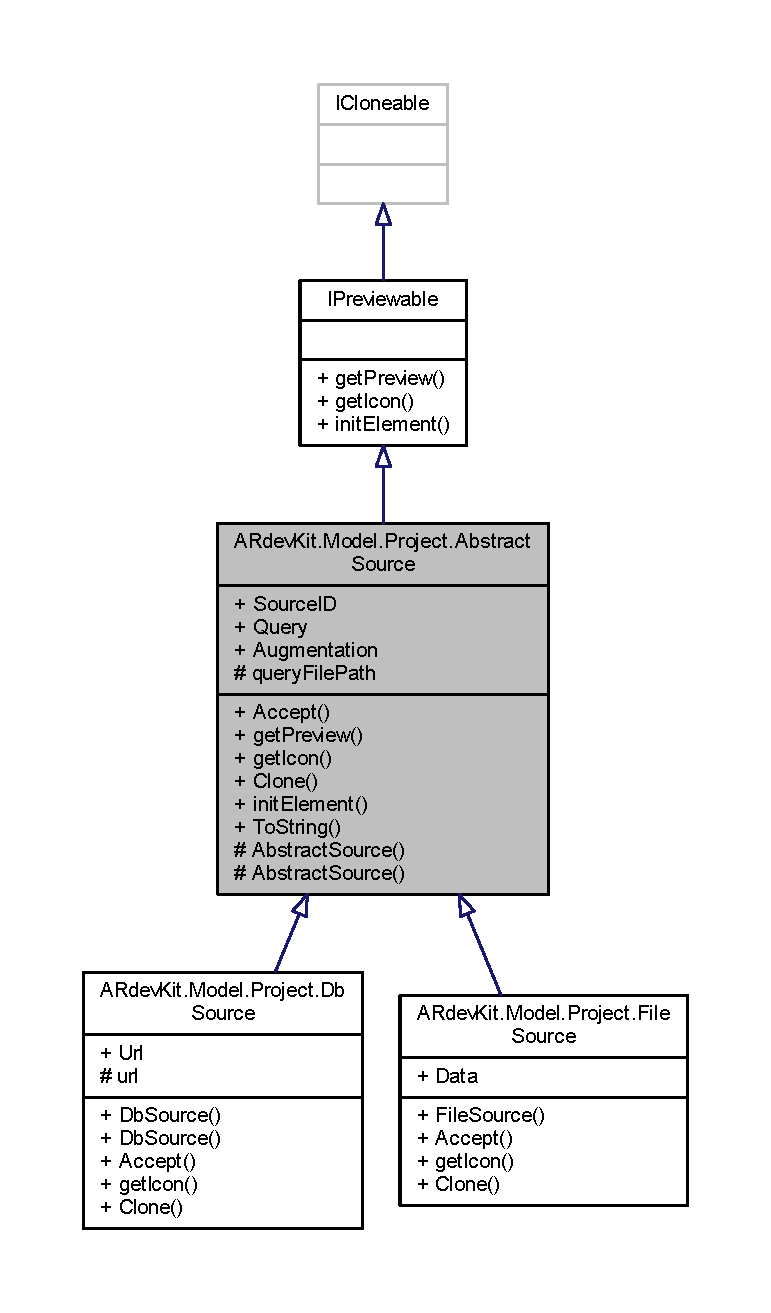
\includegraphics[height=550pt]{class_a_rdev_kit_1_1_model_1_1_project_1_1_abstract_source__inherit__graph}
\end{center}
\end{figure}


Collaboration diagram for A\-Rdev\-Kit.\-Model.\-Project.\-Abstract\-Source\-:
\nopagebreak
\begin{figure}[H]
\begin{center}
\leavevmode
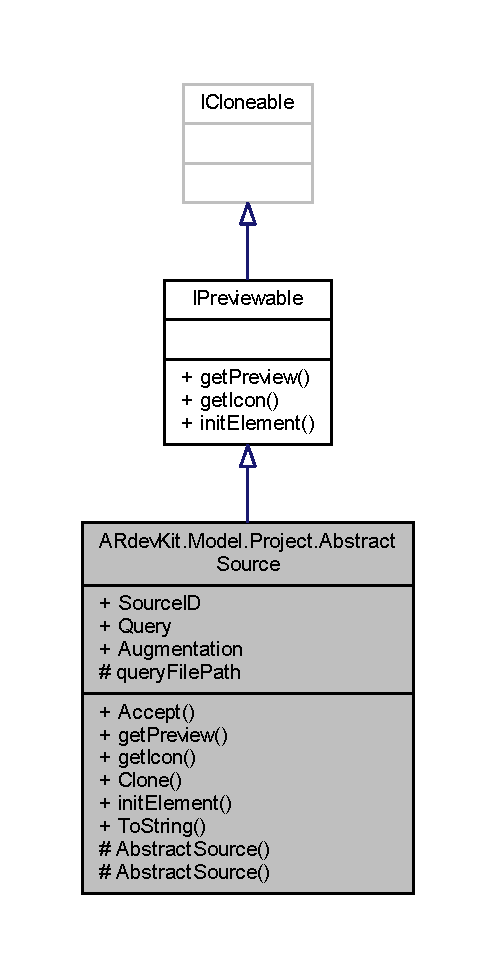
\includegraphics[width=238pt]{class_a_rdev_kit_1_1_model_1_1_project_1_1_abstract_source__coll__graph}
\end{center}
\end{figure}
\subsection*{Public Member Functions}
\begin{DoxyCompactItemize}
\item 
abstract void \hyperlink{class_a_rdev_kit_1_1_model_1_1_project_1_1_abstract_source_ad45fa69ac940512f91457ca7c7661882}{Accept} (\hyperlink{class_a_rdev_kit_1_1_controller_1_1_project_controller_1_1_abstract_project_visitor}{Abstract\-Project\-Visitor} visitor)
\begin{DoxyCompactList}\small\item\em An abstract method, to accept an Abstract\-Project\-Visitor which must be implemented according to the visitor design pattern. \end{DoxyCompactList}\item 
Bitmap \hyperlink{class_a_rdev_kit_1_1_model_1_1_project_1_1_abstract_source_abd9f742efb27a1fca992f6627c0421e4}{get\-Preview} ()
\begin{DoxyCompactList}\small\item\em returns N\-O Bitmap in order to be displayed on the Preview\-Panel, implements \hyperlink{interface_a_rdev_kit_1_1_model_1_1_project_1_1_i_previewable}{I\-Previewable} \end{DoxyCompactList}\item 
abstract Bitmap \hyperlink{class_a_rdev_kit_1_1_model_1_1_project_1_1_abstract_source_ae698f1c9d55cc0603931bd2804d0c35d}{get\-Icon} ()
\begin{DoxyCompactList}\small\item\em returns a Bitmap in order to be displayed on the Element\-Selection\-Panel, implements \hyperlink{interface_a_rdev_kit_1_1_model_1_1_project_1_1_i_previewable}{I\-Previewable} \end{DoxyCompactList}\item 
abstract object \hyperlink{class_a_rdev_kit_1_1_model_1_1_project_1_1_abstract_source_a17fb18629481715303c5c55a867bb023}{Clone} ()
\begin{DoxyCompactList}\small\item\em Makes a deep copy of this object. \end{DoxyCompactList}\item 
virtual bool \hyperlink{class_a_rdev_kit_1_1_model_1_1_project_1_1_abstract_source_ae0ad810da02d289ddcbb28bb2aabec43}{init\-Element} (\hyperlink{class_a_rdev_kit_1_1_editor_window}{Editor\-Window} ew)
\begin{DoxyCompactList}\small\item\em This method is called by the preview\-Controller when a new instance of the element is added to the Scene. It sets \char`\"{}must-\/have\char`\"{} properties. \end{DoxyCompactList}\item 
override string \hyperlink{class_a_rdev_kit_1_1_model_1_1_project_1_1_abstract_source_a74cf779ccb9c125ff5202864414f2078}{To\-String} ()
\begin{DoxyCompactList}\small\item\em Returns a System.\-String that represents this instance. \end{DoxyCompactList}\end{DoxyCompactItemize}
\subsection*{Protected Member Functions}
\begin{DoxyCompactItemize}
\item 
\hyperlink{class_a_rdev_kit_1_1_model_1_1_project_1_1_abstract_source_afbfcad1056b3776f35bdd1b09541ae28}{Abstract\-Source} ()
\begin{DoxyCompactList}\small\item\em Initializes no new instance of the \hyperlink{class_a_rdev_kit_1_1_model_1_1_project_1_1_abstract_source}{Abstract\-Source} class, \end{DoxyCompactList}\item 
\hyperlink{class_a_rdev_kit_1_1_model_1_1_project_1_1_abstract_source_a675e2b01328010a1c6d690e07ba04593}{Abstract\-Source} (string source\-Id)
\begin{DoxyCompactList}\small\item\em Initializes no new instance of the \hyperlink{class_a_rdev_kit_1_1_model_1_1_project_1_1_abstract_source}{Abstract\-Source} class. but can be used from inheriting classes. \end{DoxyCompactList}\end{DoxyCompactItemize}
\subsection*{Protected Attributes}
\begin{DoxyCompactItemize}
\item 
string \hyperlink{class_a_rdev_kit_1_1_model_1_1_project_1_1_abstract_source_abc3b4344725b8e3ae380f1922b59cf53}{query\-File\-Path}
\begin{DoxyCompactList}\small\item\em The query to the source. \end{DoxyCompactList}\end{DoxyCompactItemize}
\subsection*{Properties}
\begin{DoxyCompactItemize}
\item 
String \hyperlink{class_a_rdev_kit_1_1_model_1_1_project_1_1_abstract_source_ad17fdcfdfb0b52e0a2780e7117fd9ffc}{Source\-I\-D}\hspace{0.3cm}{\ttfamily  \mbox{[}get, set\mbox{]}}
\begin{DoxyCompactList}\small\item\em Gets or sets the source identifier. \end{DoxyCompactList}\item 
string \hyperlink{class_a_rdev_kit_1_1_model_1_1_project_1_1_abstract_source_a77b9039615be2c2792e6f6792f0d32bc}{Query}\hspace{0.3cm}{\ttfamily  \mbox{[}get, set\mbox{]}}
\begin{DoxyCompactList}\small\item\em Gets or sets the query. \end{DoxyCompactList}\item 
\hyperlink{class_a_rdev_kit_1_1_model_1_1_project_1_1_abstract_dynamic2_d_augmentation}{Abstract\-Dynamic2\-D\-Augmentation} \hyperlink{class_a_rdev_kit_1_1_model_1_1_project_1_1_abstract_source_a97697e9bd1d99e0c8a35f47a19568016}{Augmentation}\hspace{0.3cm}{\ttfamily  \mbox{[}get, set\mbox{]}}
\begin{DoxyCompactList}\small\item\em Gets or sets the augmentations, which get their dynamic information from the \hyperlink{class_a_rdev_kit_1_1_model_1_1_project_1_1_abstract_source}{Abstract\-Source} \end{DoxyCompactList}\end{DoxyCompactItemize}


\subsection{Detailed Description}
\hyperlink{class_a_rdev_kit_1_1_model_1_1_project_1_1_abstract_source}{Abstract\-Source} has no Picture\-Box in the Preview\-Panel, so it doesn't need a \hyperlink{class_a_rdev_kit_1_1_model_1_1_project_1_1_abstract_source_abd9f742efb27a1fca992f6627c0421e4}{get\-Preview()} method, though \hyperlink{class_a_rdev_kit_1_1_model_1_1_project_1_1_abstract_source_ae698f1c9d55cc0603931bd2804d0c35d}{get\-Icon()} is needed for the Element\-Selection\-Panel. 

\subsection{Constructor \& Destructor Documentation}
\hypertarget{class_a_rdev_kit_1_1_model_1_1_project_1_1_abstract_source_afbfcad1056b3776f35bdd1b09541ae28}{\index{A\-Rdev\-Kit\-::\-Model\-::\-Project\-::\-Abstract\-Source@{A\-Rdev\-Kit\-::\-Model\-::\-Project\-::\-Abstract\-Source}!Abstract\-Source@{Abstract\-Source}}
\index{Abstract\-Source@{Abstract\-Source}!ARdevKit::Model::Project::AbstractSource@{A\-Rdev\-Kit\-::\-Model\-::\-Project\-::\-Abstract\-Source}}
\subsubsection[{Abstract\-Source}]{\setlength{\rightskip}{0pt plus 5cm}A\-Rdev\-Kit.\-Model.\-Project.\-Abstract\-Source.\-Abstract\-Source (
\begin{DoxyParamCaption}
{}
\end{DoxyParamCaption}
)\hspace{0.3cm}{\ttfamily [protected]}}}\label{class_a_rdev_kit_1_1_model_1_1_project_1_1_abstract_source_afbfcad1056b3776f35bdd1b09541ae28}


Initializes no new instance of the \hyperlink{class_a_rdev_kit_1_1_model_1_1_project_1_1_abstract_source}{Abstract\-Source} class, 

\hypertarget{class_a_rdev_kit_1_1_model_1_1_project_1_1_abstract_source_a675e2b01328010a1c6d690e07ba04593}{\index{A\-Rdev\-Kit\-::\-Model\-::\-Project\-::\-Abstract\-Source@{A\-Rdev\-Kit\-::\-Model\-::\-Project\-::\-Abstract\-Source}!Abstract\-Source@{Abstract\-Source}}
\index{Abstract\-Source@{Abstract\-Source}!ARdevKit::Model::Project::AbstractSource@{A\-Rdev\-Kit\-::\-Model\-::\-Project\-::\-Abstract\-Source}}
\subsubsection[{Abstract\-Source}]{\setlength{\rightskip}{0pt plus 5cm}A\-Rdev\-Kit.\-Model.\-Project.\-Abstract\-Source.\-Abstract\-Source (
\begin{DoxyParamCaption}
\item[{string}]{source\-Id}
\end{DoxyParamCaption}
)\hspace{0.3cm}{\ttfamily [protected]}}}\label{class_a_rdev_kit_1_1_model_1_1_project_1_1_abstract_source_a675e2b01328010a1c6d690e07ba04593}


Initializes no new instance of the \hyperlink{class_a_rdev_kit_1_1_model_1_1_project_1_1_abstract_source}{Abstract\-Source} class. but can be used from inheriting classes. 


\begin{DoxyParams}{Parameters}
{\em source\-Id} & The source identifier.\\
\hline
\end{DoxyParams}


\subsection{Member Function Documentation}
\hypertarget{class_a_rdev_kit_1_1_model_1_1_project_1_1_abstract_source_ad45fa69ac940512f91457ca7c7661882}{\index{A\-Rdev\-Kit\-::\-Model\-::\-Project\-::\-Abstract\-Source@{A\-Rdev\-Kit\-::\-Model\-::\-Project\-::\-Abstract\-Source}!Accept@{Accept}}
\index{Accept@{Accept}!ARdevKit::Model::Project::AbstractSource@{A\-Rdev\-Kit\-::\-Model\-::\-Project\-::\-Abstract\-Source}}
\subsubsection[{Accept}]{\setlength{\rightskip}{0pt plus 5cm}abstract void A\-Rdev\-Kit.\-Model.\-Project.\-Abstract\-Source.\-Accept (
\begin{DoxyParamCaption}
\item[{{\bf Abstract\-Project\-Visitor}}]{visitor}
\end{DoxyParamCaption}
)\hspace{0.3cm}{\ttfamily [pure virtual]}}}\label{class_a_rdev_kit_1_1_model_1_1_project_1_1_abstract_source_ad45fa69ac940512f91457ca7c7661882}


An abstract method, to accept an Abstract\-Project\-Visitor which must be implemented according to the visitor design pattern. 


\begin{DoxyParams}{Parameters}
{\em visitor} & the visitor which encapsulates the action which is performed on this element\\
\hline
\end{DoxyParams}


Implemented in \hyperlink{class_a_rdev_kit_1_1_model_1_1_project_1_1_db_source_aaa7e395578b8e983de0392dd37c55c93}{A\-Rdev\-Kit.\-Model.\-Project.\-Db\-Source}.

\hypertarget{class_a_rdev_kit_1_1_model_1_1_project_1_1_abstract_source_a17fb18629481715303c5c55a867bb023}{\index{A\-Rdev\-Kit\-::\-Model\-::\-Project\-::\-Abstract\-Source@{A\-Rdev\-Kit\-::\-Model\-::\-Project\-::\-Abstract\-Source}!Clone@{Clone}}
\index{Clone@{Clone}!ARdevKit::Model::Project::AbstractSource@{A\-Rdev\-Kit\-::\-Model\-::\-Project\-::\-Abstract\-Source}}
\subsubsection[{Clone}]{\setlength{\rightskip}{0pt plus 5cm}abstract object A\-Rdev\-Kit.\-Model.\-Project.\-Abstract\-Source.\-Clone (
\begin{DoxyParamCaption}
{}
\end{DoxyParamCaption}
)\hspace{0.3cm}{\ttfamily [pure virtual]}}}\label{class_a_rdev_kit_1_1_model_1_1_project_1_1_abstract_source_a17fb18629481715303c5c55a867bb023}


Makes a deep copy of this object. 

Robin, 22.\-01.\-2014. 

\begin{DoxyReturn}{Returns}
A copy of this object. 
\end{DoxyReturn}


Implemented in \hyperlink{class_a_rdev_kit_1_1_model_1_1_project_1_1_db_source_a9c58ffefa3fd6d23d58392273be07d17}{A\-Rdev\-Kit.\-Model.\-Project.\-Db\-Source}, and \hyperlink{class_a_rdev_kit_1_1_model_1_1_project_1_1_file_source_ac97ee603e5e8f17bea48dc1d81e7b531}{A\-Rdev\-Kit.\-Model.\-Project.\-File\-Source}.

\hypertarget{class_a_rdev_kit_1_1_model_1_1_project_1_1_abstract_source_ae698f1c9d55cc0603931bd2804d0c35d}{\index{A\-Rdev\-Kit\-::\-Model\-::\-Project\-::\-Abstract\-Source@{A\-Rdev\-Kit\-::\-Model\-::\-Project\-::\-Abstract\-Source}!get\-Icon@{get\-Icon}}
\index{get\-Icon@{get\-Icon}!ARdevKit::Model::Project::AbstractSource@{A\-Rdev\-Kit\-::\-Model\-::\-Project\-::\-Abstract\-Source}}
\subsubsection[{get\-Icon}]{\setlength{\rightskip}{0pt plus 5cm}abstract Bitmap A\-Rdev\-Kit.\-Model.\-Project.\-Abstract\-Source.\-get\-Icon (
\begin{DoxyParamCaption}
{}
\end{DoxyParamCaption}
)\hspace{0.3cm}{\ttfamily [pure virtual]}}}\label{class_a_rdev_kit_1_1_model_1_1_project_1_1_abstract_source_ae698f1c9d55cc0603931bd2804d0c35d}


returns a Bitmap in order to be displayed on the Element\-Selection\-Panel, implements \hyperlink{interface_a_rdev_kit_1_1_model_1_1_project_1_1_i_previewable}{I\-Previewable} 

\begin{DoxyReturn}{Returns}
a representative iconized Bitmap
\end{DoxyReturn}


Implements \hyperlink{interface_a_rdev_kit_1_1_model_1_1_project_1_1_i_previewable_a8573bdaccd5227400b538c34c1b5f279}{A\-Rdev\-Kit.\-Model.\-Project.\-I\-Previewable}.



Implemented in \hyperlink{class_a_rdev_kit_1_1_model_1_1_project_1_1_db_source_a0890127d66db4ce9c3daa6fe6f44f157}{A\-Rdev\-Kit.\-Model.\-Project.\-Db\-Source}, and \hyperlink{class_a_rdev_kit_1_1_model_1_1_project_1_1_file_source_a1c35e8b945898af5787b60f3de7a2d26}{A\-Rdev\-Kit.\-Model.\-Project.\-File\-Source}.

\hypertarget{class_a_rdev_kit_1_1_model_1_1_project_1_1_abstract_source_abd9f742efb27a1fca992f6627c0421e4}{\index{A\-Rdev\-Kit\-::\-Model\-::\-Project\-::\-Abstract\-Source@{A\-Rdev\-Kit\-::\-Model\-::\-Project\-::\-Abstract\-Source}!get\-Preview@{get\-Preview}}
\index{get\-Preview@{get\-Preview}!ARdevKit::Model::Project::AbstractSource@{A\-Rdev\-Kit\-::\-Model\-::\-Project\-::\-Abstract\-Source}}
\subsubsection[{get\-Preview}]{\setlength{\rightskip}{0pt plus 5cm}Bitmap A\-Rdev\-Kit.\-Model.\-Project.\-Abstract\-Source.\-get\-Preview (
\begin{DoxyParamCaption}
{}
\end{DoxyParamCaption}
)}}\label{class_a_rdev_kit_1_1_model_1_1_project_1_1_abstract_source_abd9f742efb27a1fca992f6627c0421e4}


returns N\-O Bitmap in order to be displayed on the Preview\-Panel, implements \hyperlink{interface_a_rdev_kit_1_1_model_1_1_project_1_1_i_previewable}{I\-Previewable} 

\begin{DoxyReturn}{Returns}

\end{DoxyReturn}

\begin{DoxyExceptions}{Exceptions}
{\em System.\-Not\-Supported\-Exception} & \\
\hline
{\em Not\-Supported\-Exception} & \\
\hline
\end{DoxyExceptions}


Implements \hyperlink{interface_a_rdev_kit_1_1_model_1_1_project_1_1_i_previewable_a7cbcbb20929f4f1b6db3321ed2e83070}{A\-Rdev\-Kit.\-Model.\-Project.\-I\-Previewable}.

\hypertarget{class_a_rdev_kit_1_1_model_1_1_project_1_1_abstract_source_ae0ad810da02d289ddcbb28bb2aabec43}{\index{A\-Rdev\-Kit\-::\-Model\-::\-Project\-::\-Abstract\-Source@{A\-Rdev\-Kit\-::\-Model\-::\-Project\-::\-Abstract\-Source}!init\-Element@{init\-Element}}
\index{init\-Element@{init\-Element}!ARdevKit::Model::Project::AbstractSource@{A\-Rdev\-Kit\-::\-Model\-::\-Project\-::\-Abstract\-Source}}
\subsubsection[{init\-Element}]{\setlength{\rightskip}{0pt plus 5cm}virtual bool A\-Rdev\-Kit.\-Model.\-Project.\-Abstract\-Source.\-init\-Element (
\begin{DoxyParamCaption}
\item[{{\bf Editor\-Window}}]{ew}
\end{DoxyParamCaption}
)\hspace{0.3cm}{\ttfamily [virtual]}}}\label{class_a_rdev_kit_1_1_model_1_1_project_1_1_abstract_source_ae0ad810da02d289ddcbb28bb2aabec43}


This method is called by the preview\-Controller when a new instance of the element is added to the Scene. It sets \char`\"{}must-\/have\char`\"{} properties. 


\begin{DoxyParams}{Parameters}
{\em ew} & The ew.\\
\hline
\end{DoxyParams}
\begin{DoxyReturn}{Returns}
true if it succeeds, false if it fails. 
\end{DoxyReturn}


Implements \hyperlink{interface_a_rdev_kit_1_1_model_1_1_project_1_1_i_previewable_aa638e27d88c30b7e63b241d1001042c9}{A\-Rdev\-Kit.\-Model.\-Project.\-I\-Previewable}.

\hypertarget{class_a_rdev_kit_1_1_model_1_1_project_1_1_abstract_source_a74cf779ccb9c125ff5202864414f2078}{\index{A\-Rdev\-Kit\-::\-Model\-::\-Project\-::\-Abstract\-Source@{A\-Rdev\-Kit\-::\-Model\-::\-Project\-::\-Abstract\-Source}!To\-String@{To\-String}}
\index{To\-String@{To\-String}!ARdevKit::Model::Project::AbstractSource@{A\-Rdev\-Kit\-::\-Model\-::\-Project\-::\-Abstract\-Source}}
\subsubsection[{To\-String}]{\setlength{\rightskip}{0pt plus 5cm}override string A\-Rdev\-Kit.\-Model.\-Project.\-Abstract\-Source.\-To\-String (
\begin{DoxyParamCaption}
{}
\end{DoxyParamCaption}
)}}\label{class_a_rdev_kit_1_1_model_1_1_project_1_1_abstract_source_a74cf779ccb9c125ff5202864414f2078}


Returns a System.\-String that represents this instance. 

\begin{DoxyReturn}{Returns}
A System.\-String that represents this instance. 
\end{DoxyReturn}


\subsection{Member Data Documentation}
\hypertarget{class_a_rdev_kit_1_1_model_1_1_project_1_1_abstract_source_abc3b4344725b8e3ae380f1922b59cf53}{\index{A\-Rdev\-Kit\-::\-Model\-::\-Project\-::\-Abstract\-Source@{A\-Rdev\-Kit\-::\-Model\-::\-Project\-::\-Abstract\-Source}!query\-File\-Path@{query\-File\-Path}}
\index{query\-File\-Path@{query\-File\-Path}!ARdevKit::Model::Project::AbstractSource@{A\-Rdev\-Kit\-::\-Model\-::\-Project\-::\-Abstract\-Source}}
\subsubsection[{query\-File\-Path}]{\setlength{\rightskip}{0pt plus 5cm}string A\-Rdev\-Kit.\-Model.\-Project.\-Abstract\-Source.\-query\-File\-Path\hspace{0.3cm}{\ttfamily [protected]}}}\label{class_a_rdev_kit_1_1_model_1_1_project_1_1_abstract_source_abc3b4344725b8e3ae380f1922b59cf53}


The query to the source. 



\subsection{Property Documentation}
\hypertarget{class_a_rdev_kit_1_1_model_1_1_project_1_1_abstract_source_a97697e9bd1d99e0c8a35f47a19568016}{\index{A\-Rdev\-Kit\-::\-Model\-::\-Project\-::\-Abstract\-Source@{A\-Rdev\-Kit\-::\-Model\-::\-Project\-::\-Abstract\-Source}!Augmentation@{Augmentation}}
\index{Augmentation@{Augmentation}!ARdevKit::Model::Project::AbstractSource@{A\-Rdev\-Kit\-::\-Model\-::\-Project\-::\-Abstract\-Source}}
\subsubsection[{Augmentation}]{\setlength{\rightskip}{0pt plus 5cm}{\bf Abstract\-Dynamic2\-D\-Augmentation} A\-Rdev\-Kit.\-Model.\-Project.\-Abstract\-Source.\-Augmentation\hspace{0.3cm}{\ttfamily [get]}, {\ttfamily [set]}}}\label{class_a_rdev_kit_1_1_model_1_1_project_1_1_abstract_source_a97697e9bd1d99e0c8a35f47a19568016}


Gets or sets the augmentations, which get their dynamic information from the \hyperlink{class_a_rdev_kit_1_1_model_1_1_project_1_1_abstract_source}{Abstract\-Source} 

The augmentations. \hypertarget{class_a_rdev_kit_1_1_model_1_1_project_1_1_abstract_source_a77b9039615be2c2792e6f6792f0d32bc}{\index{A\-Rdev\-Kit\-::\-Model\-::\-Project\-::\-Abstract\-Source@{A\-Rdev\-Kit\-::\-Model\-::\-Project\-::\-Abstract\-Source}!Query@{Query}}
\index{Query@{Query}!ARdevKit::Model::Project::AbstractSource@{A\-Rdev\-Kit\-::\-Model\-::\-Project\-::\-Abstract\-Source}}
\subsubsection[{Query}]{\setlength{\rightskip}{0pt plus 5cm}string A\-Rdev\-Kit.\-Model.\-Project.\-Abstract\-Source.\-Query\hspace{0.3cm}{\ttfamily [get]}, {\ttfamily [set]}}}\label{class_a_rdev_kit_1_1_model_1_1_project_1_1_abstract_source_a77b9039615be2c2792e6f6792f0d32bc}


Gets or sets the query. 

The query. \hypertarget{class_a_rdev_kit_1_1_model_1_1_project_1_1_abstract_source_ad17fdcfdfb0b52e0a2780e7117fd9ffc}{\index{A\-Rdev\-Kit\-::\-Model\-::\-Project\-::\-Abstract\-Source@{A\-Rdev\-Kit\-::\-Model\-::\-Project\-::\-Abstract\-Source}!Source\-I\-D@{Source\-I\-D}}
\index{Source\-I\-D@{Source\-I\-D}!ARdevKit::Model::Project::AbstractSource@{A\-Rdev\-Kit\-::\-Model\-::\-Project\-::\-Abstract\-Source}}
\subsubsection[{Source\-I\-D}]{\setlength{\rightskip}{0pt plus 5cm}String A\-Rdev\-Kit.\-Model.\-Project.\-Abstract\-Source.\-Source\-I\-D\hspace{0.3cm}{\ttfamily [get]}, {\ttfamily [set]}}}\label{class_a_rdev_kit_1_1_model_1_1_project_1_1_abstract_source_ad17fdcfdfb0b52e0a2780e7117fd9ffc}


Gets or sets the source identifier. 

The source identifier. 
\hypertarget{class_a_rdev_kit_1_1_model_1_1_project_1_1_abstract_trackable}{\section{A\-Rdev\-Kit.\-Model.\-Project.\-Abstract\-Trackable Class Reference}
\label{class_a_rdev_kit_1_1_model_1_1_project_1_1_abstract_trackable}\index{A\-Rdev\-Kit.\-Model.\-Project.\-Abstract\-Trackable@{A\-Rdev\-Kit.\-Model.\-Project.\-Abstract\-Trackable}}
}


Describes an \hyperlink{class_a_rdev_kit_1_1_model_1_1_project_1_1_abstract_trackable}{Abstract\-Trackable} with its associated \hyperlink{class_a_rdev_kit_1_1_model_1_1_project_1_1_abstract_augmentation}{Abstract\-Augmentation}s and further details used for A\-R\-E\-L. Is \hyperlink{interface_a_rdev_kit_1_1_model_1_1_project_1_1_i_previewable}{I\-Previewable}  




Inheritance diagram for A\-Rdev\-Kit.\-Model.\-Project.\-Abstract\-Trackable\-:
\nopagebreak
\begin{figure}[H]
\begin{center}
\leavevmode
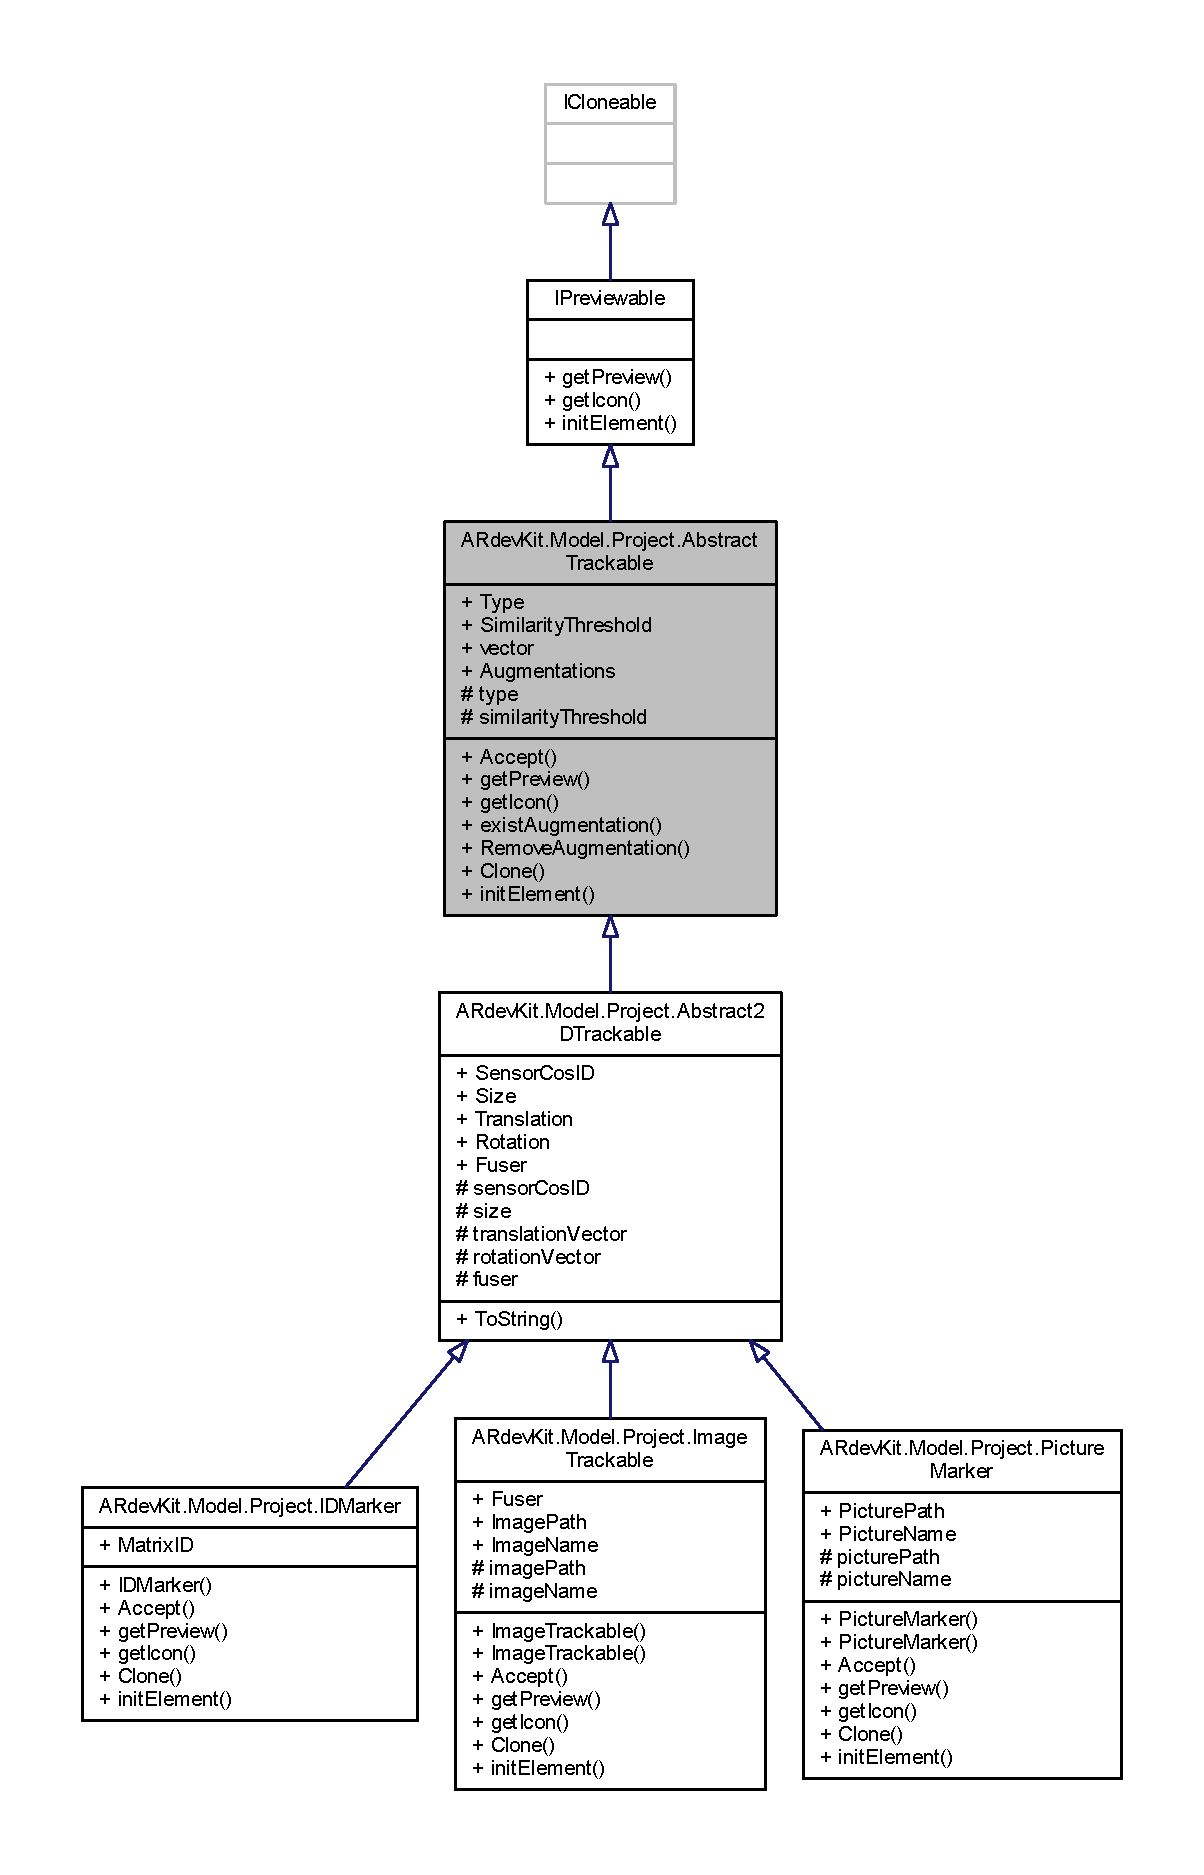
\includegraphics[width=350pt]{class_a_rdev_kit_1_1_model_1_1_project_1_1_abstract_trackable__inherit__graph}
\end{center}
\end{figure}


Collaboration diagram for A\-Rdev\-Kit.\-Model.\-Project.\-Abstract\-Trackable\-:
\nopagebreak
\begin{figure}[H]
\begin{center}
\leavevmode
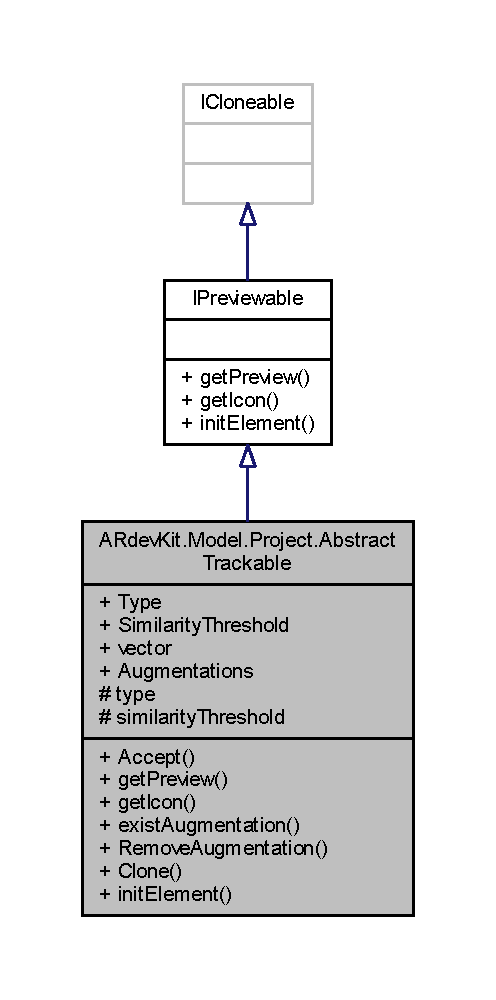
\includegraphics[width=238pt]{class_a_rdev_kit_1_1_model_1_1_project_1_1_abstract_trackable__coll__graph}
\end{center}
\end{figure}
\subsection*{Public Member Functions}
\begin{DoxyCompactItemize}
\item 
abstract void \hyperlink{class_a_rdev_kit_1_1_model_1_1_project_1_1_abstract_trackable_a76f6ad0ed8f615b8f5b7738411abb54f}{Accept} (\hyperlink{class_a_rdev_kit_1_1_controller_1_1_project_controller_1_1_abstract_project_visitor}{Abstract\-Project\-Visitor} visitor)
\begin{DoxyCompactList}\small\item\em An abstract method, to accept a Abstract\-Project\-Visitor which must be implemented according to the visitor design pattern. \end{DoxyCompactList}\item 
abstract Bitmap \hyperlink{class_a_rdev_kit_1_1_model_1_1_project_1_1_abstract_trackable_ab4d8a1902c82fe7a1d385d5688f92bd8}{get\-Preview} ()
\begin{DoxyCompactList}\small\item\em returns a Bitmap in order to be displayed on the Preview\-Panel, implements \hyperlink{interface_a_rdev_kit_1_1_model_1_1_project_1_1_i_previewable}{I\-Previewable} \end{DoxyCompactList}\item 
abstract Bitmap \hyperlink{class_a_rdev_kit_1_1_model_1_1_project_1_1_abstract_trackable_abee7e96dac48f6fa7fc424c0f9139dff}{get\-Icon} ()
\begin{DoxyCompactList}\small\item\em returns a Bitmap in order to be displayed on the Element\-Selection\-Panel, implements \hyperlink{interface_a_rdev_kit_1_1_model_1_1_project_1_1_i_previewable}{I\-Previewable} \end{DoxyCompactList}\item 
bool \hyperlink{class_a_rdev_kit_1_1_model_1_1_project_1_1_abstract_trackable_ac5dfdc39c3e7ad91ca9156208278b108}{exist\-Augmentation} (\hyperlink{interface_a_rdev_kit_1_1_model_1_1_project_1_1_i_previewable}{I\-Previewable} a)
\begin{DoxyCompactList}\small\item\em Checks if the augmentation is associated with this \hyperlink{class_a_rdev_kit_1_1_model_1_1_project_1_1_abstract_trackable}{Abstract\-Trackable}. \end{DoxyCompactList}\item 
void \hyperlink{class_a_rdev_kit_1_1_model_1_1_project_1_1_abstract_trackable_ae14b72d85d610bcda17d93255bce45f7}{Remove\-Augmentation} (\hyperlink{class_a_rdev_kit_1_1_model_1_1_project_1_1_abstract_augmentation}{Abstract\-Augmentation} augmentation)
\begin{DoxyCompactList}\small\item\em Removes the augmentation described by augmentation. \end{DoxyCompactList}\item 
abstract object \hyperlink{class_a_rdev_kit_1_1_model_1_1_project_1_1_abstract_trackable_a166fc03dc00911591baca14a3341ef29}{Clone} ()
\begin{DoxyCompactList}\small\item\em Makes a deep copy of this object. \end{DoxyCompactList}\item 
virtual bool \hyperlink{class_a_rdev_kit_1_1_model_1_1_project_1_1_abstract_trackable_aff50ed9cb95973d56d6a65bd1ef96c0a}{init\-Element} (\hyperlink{class_a_rdev_kit_1_1_editor_window}{Editor\-Window} ew)
\begin{DoxyCompactList}\small\item\em This method is called by the preview\-Controller when a new instance of the element is added to the Scene. It sets \char`\"{}must-\/have\char`\"{} properties. \end{DoxyCompactList}\end{DoxyCompactItemize}
\subsection*{Protected Attributes}
\begin{DoxyCompactItemize}
\item 
string \hyperlink{class_a_rdev_kit_1_1_model_1_1_project_1_1_abstract_trackable_ab6faf8843d1e9a61b353286a8d583231}{type}
\begin{DoxyCompactList}\small\item\em The type, to differtiate between different Marker types and their way to be tracked. \end{DoxyCompactList}\item 
double \hyperlink{class_a_rdev_kit_1_1_model_1_1_project_1_1_abstract_trackable_a5a74b70a54b9bb1f4fbad46e08a2e0cd}{similarity\-Threshold}
\begin{DoxyCompactList}\small\item\em Describes at which similarity, a picture recorded by the camera is recognized to be the desired one. Only experts usage. \end{DoxyCompactList}\end{DoxyCompactItemize}
\subsection*{Properties}
\begin{DoxyCompactItemize}
\item 
string \hyperlink{class_a_rdev_kit_1_1_model_1_1_project_1_1_abstract_trackable_ab55c05790e5ffbefc7351a91167427bc}{Type}\hspace{0.3cm}{\ttfamily  \mbox{[}get, set\mbox{]}}
\begin{DoxyCompactList}\small\item\em Gets or sets the type. \end{DoxyCompactList}\item 
double \hyperlink{class_a_rdev_kit_1_1_model_1_1_project_1_1_abstract_trackable_af77b1f7a449ef9150e22c684894213b1}{Similarity\-Threshold}\hspace{0.3cm}{\ttfamily  \mbox{[}get, set\mbox{]}}
\begin{DoxyCompactList}\small\item\em Gets or sets the similarity threshold. \end{DoxyCompactList}\item 
\hyperlink{class_a_rdev_kit_1_1_model_1_1_project_1_1_vector3_d}{Vector3\-D} \hyperlink{class_a_rdev_kit_1_1_model_1_1_project_1_1_abstract_trackable_a1a8b6d43d95fad1720fc5af98b7e42b4}{vector}\hspace{0.3cm}{\ttfamily  \mbox{[}get, set\mbox{]}}
\begin{DoxyCompactList}\small\item\em Describes the position of the Trackable in the coordinatesystem used by metaio. \end{DoxyCompactList}\item 
List$<$ \hyperlink{class_a_rdev_kit_1_1_model_1_1_project_1_1_abstract_augmentation}{Abstract\-Augmentation} $>$ \hyperlink{class_a_rdev_kit_1_1_model_1_1_project_1_1_abstract_trackable_a999faeee63dee9445e8617d539c5b8d9}{Augmentations}\hspace{0.3cm}{\ttfamily  \mbox{[}get, set\mbox{]}}
\begin{DoxyCompactList}\small\item\em Lists all associated Abstract\-Augmentations. \end{DoxyCompactList}\end{DoxyCompactItemize}


\subsection{Detailed Description}
Describes an \hyperlink{class_a_rdev_kit_1_1_model_1_1_project_1_1_abstract_trackable}{Abstract\-Trackable} with its associated \hyperlink{class_a_rdev_kit_1_1_model_1_1_project_1_1_abstract_augmentation}{Abstract\-Augmentation}s and further details used for A\-R\-E\-L. Is \hyperlink{interface_a_rdev_kit_1_1_model_1_1_project_1_1_i_previewable}{I\-Previewable} 



\subsection{Member Function Documentation}
\hypertarget{class_a_rdev_kit_1_1_model_1_1_project_1_1_abstract_trackable_a76f6ad0ed8f615b8f5b7738411abb54f}{\index{A\-Rdev\-Kit\-::\-Model\-::\-Project\-::\-Abstract\-Trackable@{A\-Rdev\-Kit\-::\-Model\-::\-Project\-::\-Abstract\-Trackable}!Accept@{Accept}}
\index{Accept@{Accept}!ARdevKit::Model::Project::AbstractTrackable@{A\-Rdev\-Kit\-::\-Model\-::\-Project\-::\-Abstract\-Trackable}}
\subsubsection[{Accept}]{\setlength{\rightskip}{0pt plus 5cm}abstract void A\-Rdev\-Kit.\-Model.\-Project.\-Abstract\-Trackable.\-Accept (
\begin{DoxyParamCaption}
\item[{{\bf Abstract\-Project\-Visitor}}]{visitor}
\end{DoxyParamCaption}
)\hspace{0.3cm}{\ttfamily [pure virtual]}}}\label{class_a_rdev_kit_1_1_model_1_1_project_1_1_abstract_trackable_a76f6ad0ed8f615b8f5b7738411abb54f}


An abstract method, to accept a Abstract\-Project\-Visitor which must be implemented according to the visitor design pattern. 


\begin{DoxyParams}{Parameters}
{\em visitor} & the visitor which encapsulates the action which is performed on this element\\
\hline
\end{DoxyParams}


Implemented in \hyperlink{class_a_rdev_kit_1_1_model_1_1_project_1_1_picture_marker_a9f06478c438150cd695dc8db8140b913}{A\-Rdev\-Kit.\-Model.\-Project.\-Picture\-Marker}.

\hypertarget{class_a_rdev_kit_1_1_model_1_1_project_1_1_abstract_trackable_a166fc03dc00911591baca14a3341ef29}{\index{A\-Rdev\-Kit\-::\-Model\-::\-Project\-::\-Abstract\-Trackable@{A\-Rdev\-Kit\-::\-Model\-::\-Project\-::\-Abstract\-Trackable}!Clone@{Clone}}
\index{Clone@{Clone}!ARdevKit::Model::Project::AbstractTrackable@{A\-Rdev\-Kit\-::\-Model\-::\-Project\-::\-Abstract\-Trackable}}
\subsubsection[{Clone}]{\setlength{\rightskip}{0pt plus 5cm}abstract object A\-Rdev\-Kit.\-Model.\-Project.\-Abstract\-Trackable.\-Clone (
\begin{DoxyParamCaption}
{}
\end{DoxyParamCaption}
)\hspace{0.3cm}{\ttfamily [pure virtual]}}}\label{class_a_rdev_kit_1_1_model_1_1_project_1_1_abstract_trackable_a166fc03dc00911591baca14a3341ef29}


Makes a deep copy of this object. 

Robin, 22.\-01.\-2014. 

\begin{DoxyReturn}{Returns}
A copy of this object. 
\end{DoxyReturn}


Implemented in \hyperlink{class_a_rdev_kit_1_1_model_1_1_project_1_1_picture_marker_a090e0af9c7cdd270248516fe645b345d}{A\-Rdev\-Kit.\-Model.\-Project.\-Picture\-Marker}, \hyperlink{class_a_rdev_kit_1_1_model_1_1_project_1_1_image_trackable_a9f0502ccb4306c88c4b15793b0d1c0ba}{A\-Rdev\-Kit.\-Model.\-Project.\-Image\-Trackable}, and \hyperlink{class_a_rdev_kit_1_1_model_1_1_project_1_1_i_d_marker_a69480e66c9a3755dfb94bb7b957c18d8}{A\-Rdev\-Kit.\-Model.\-Project.\-I\-D\-Marker}.

\hypertarget{class_a_rdev_kit_1_1_model_1_1_project_1_1_abstract_trackable_ac5dfdc39c3e7ad91ca9156208278b108}{\index{A\-Rdev\-Kit\-::\-Model\-::\-Project\-::\-Abstract\-Trackable@{A\-Rdev\-Kit\-::\-Model\-::\-Project\-::\-Abstract\-Trackable}!exist\-Augmentation@{exist\-Augmentation}}
\index{exist\-Augmentation@{exist\-Augmentation}!ARdevKit::Model::Project::AbstractTrackable@{A\-Rdev\-Kit\-::\-Model\-::\-Project\-::\-Abstract\-Trackable}}
\subsubsection[{exist\-Augmentation}]{\setlength{\rightskip}{0pt plus 5cm}bool A\-Rdev\-Kit.\-Model.\-Project.\-Abstract\-Trackable.\-exist\-Augmentation (
\begin{DoxyParamCaption}
\item[{{\bf I\-Previewable}}]{a}
\end{DoxyParamCaption}
)}}\label{class_a_rdev_kit_1_1_model_1_1_project_1_1_abstract_trackable_ac5dfdc39c3e7ad91ca9156208278b108}


Checks if the augmentation is associated with this \hyperlink{class_a_rdev_kit_1_1_model_1_1_project_1_1_abstract_trackable}{Abstract\-Trackable}. 


\begin{DoxyParams}{Parameters}
{\em a} & the \hyperlink{interface_a_rdev_kit_1_1_model_1_1_project_1_1_i_previewable}{I\-Previewable}, which is checked existence for\\
\hline
\end{DoxyParams}
\begin{DoxyReturn}{Returns}
true, if its associated with this \hyperlink{class_a_rdev_kit_1_1_model_1_1_project_1_1_abstract_trackable}{Abstract\-Trackable} false, else
\end{DoxyReturn}


Here is the caller graph for this function\-:
\nopagebreak
\begin{figure}[H]
\begin{center}
\leavevmode
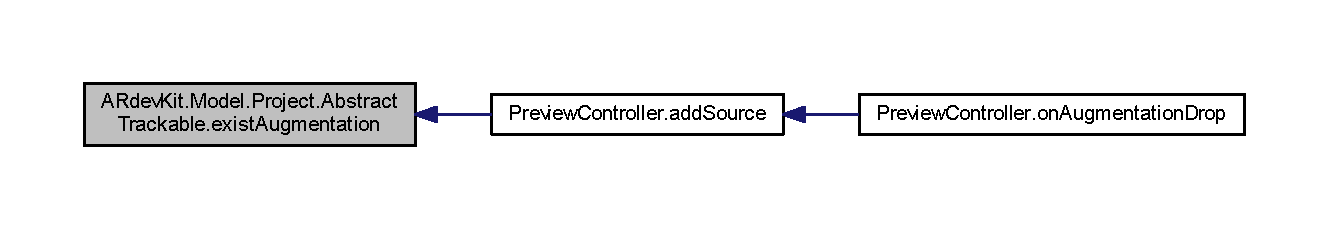
\includegraphics[width=350pt]{class_a_rdev_kit_1_1_model_1_1_project_1_1_abstract_trackable_ac5dfdc39c3e7ad91ca9156208278b108_icgraph}
\end{center}
\end{figure}


\hypertarget{class_a_rdev_kit_1_1_model_1_1_project_1_1_abstract_trackable_abee7e96dac48f6fa7fc424c0f9139dff}{\index{A\-Rdev\-Kit\-::\-Model\-::\-Project\-::\-Abstract\-Trackable@{A\-Rdev\-Kit\-::\-Model\-::\-Project\-::\-Abstract\-Trackable}!get\-Icon@{get\-Icon}}
\index{get\-Icon@{get\-Icon}!ARdevKit::Model::Project::AbstractTrackable@{A\-Rdev\-Kit\-::\-Model\-::\-Project\-::\-Abstract\-Trackable}}
\subsubsection[{get\-Icon}]{\setlength{\rightskip}{0pt plus 5cm}abstract Bitmap A\-Rdev\-Kit.\-Model.\-Project.\-Abstract\-Trackable.\-get\-Icon (
\begin{DoxyParamCaption}
{}
\end{DoxyParamCaption}
)\hspace{0.3cm}{\ttfamily [pure virtual]}}}\label{class_a_rdev_kit_1_1_model_1_1_project_1_1_abstract_trackable_abee7e96dac48f6fa7fc424c0f9139dff}


returns a Bitmap in order to be displayed on the Element\-Selection\-Panel, implements \hyperlink{interface_a_rdev_kit_1_1_model_1_1_project_1_1_i_previewable}{I\-Previewable} 

\begin{DoxyReturn}{Returns}
a representative iconized Bitmap
\end{DoxyReturn}


Implements \hyperlink{interface_a_rdev_kit_1_1_model_1_1_project_1_1_i_previewable_a8573bdaccd5227400b538c34c1b5f279}{A\-Rdev\-Kit.\-Model.\-Project.\-I\-Previewable}.



Implemented in \hyperlink{class_a_rdev_kit_1_1_model_1_1_project_1_1_picture_marker_acf5e1189f44cc8e1d42964e3842d3769}{A\-Rdev\-Kit.\-Model.\-Project.\-Picture\-Marker}, \hyperlink{class_a_rdev_kit_1_1_model_1_1_project_1_1_image_trackable_af11655160fd026f62dca5948cdf630cd}{A\-Rdev\-Kit.\-Model.\-Project.\-Image\-Trackable}, and \hyperlink{class_a_rdev_kit_1_1_model_1_1_project_1_1_i_d_marker_ae3713212fbac546d841e3be2ccb43db9}{A\-Rdev\-Kit.\-Model.\-Project.\-I\-D\-Marker}.

\hypertarget{class_a_rdev_kit_1_1_model_1_1_project_1_1_abstract_trackable_ab4d8a1902c82fe7a1d385d5688f92bd8}{\index{A\-Rdev\-Kit\-::\-Model\-::\-Project\-::\-Abstract\-Trackable@{A\-Rdev\-Kit\-::\-Model\-::\-Project\-::\-Abstract\-Trackable}!get\-Preview@{get\-Preview}}
\index{get\-Preview@{get\-Preview}!ARdevKit::Model::Project::AbstractTrackable@{A\-Rdev\-Kit\-::\-Model\-::\-Project\-::\-Abstract\-Trackable}}
\subsubsection[{get\-Preview}]{\setlength{\rightskip}{0pt plus 5cm}abstract Bitmap A\-Rdev\-Kit.\-Model.\-Project.\-Abstract\-Trackable.\-get\-Preview (
\begin{DoxyParamCaption}
{}
\end{DoxyParamCaption}
)\hspace{0.3cm}{\ttfamily [pure virtual]}}}\label{class_a_rdev_kit_1_1_model_1_1_project_1_1_abstract_trackable_ab4d8a1902c82fe7a1d385d5688f92bd8}


returns a Bitmap in order to be displayed on the Preview\-Panel, implements \hyperlink{interface_a_rdev_kit_1_1_model_1_1_project_1_1_i_previewable}{I\-Previewable} 

\begin{DoxyReturn}{Returns}
a representative Bitmap
\end{DoxyReturn}


Implements \hyperlink{interface_a_rdev_kit_1_1_model_1_1_project_1_1_i_previewable_a7cbcbb20929f4f1b6db3321ed2e83070}{A\-Rdev\-Kit.\-Model.\-Project.\-I\-Previewable}.



Implemented in \hyperlink{class_a_rdev_kit_1_1_model_1_1_project_1_1_image_trackable_a96e42ce5c75d50a49b617d8eb8f87b99}{A\-Rdev\-Kit.\-Model.\-Project.\-Image\-Trackable}, \hyperlink{class_a_rdev_kit_1_1_model_1_1_project_1_1_picture_marker_a9d608a1d9abb84c8109b7f34efffc658}{A\-Rdev\-Kit.\-Model.\-Project.\-Picture\-Marker}, and \hyperlink{class_a_rdev_kit_1_1_model_1_1_project_1_1_i_d_marker_a4533a46611ee75747a5cf96f3fc2586c}{A\-Rdev\-Kit.\-Model.\-Project.\-I\-D\-Marker}.

\hypertarget{class_a_rdev_kit_1_1_model_1_1_project_1_1_abstract_trackable_aff50ed9cb95973d56d6a65bd1ef96c0a}{\index{A\-Rdev\-Kit\-::\-Model\-::\-Project\-::\-Abstract\-Trackable@{A\-Rdev\-Kit\-::\-Model\-::\-Project\-::\-Abstract\-Trackable}!init\-Element@{init\-Element}}
\index{init\-Element@{init\-Element}!ARdevKit::Model::Project::AbstractTrackable@{A\-Rdev\-Kit\-::\-Model\-::\-Project\-::\-Abstract\-Trackable}}
\subsubsection[{init\-Element}]{\setlength{\rightskip}{0pt plus 5cm}virtual bool A\-Rdev\-Kit.\-Model.\-Project.\-Abstract\-Trackable.\-init\-Element (
\begin{DoxyParamCaption}
\item[{{\bf Editor\-Window}}]{ew}
\end{DoxyParamCaption}
)\hspace{0.3cm}{\ttfamily [virtual]}}}\label{class_a_rdev_kit_1_1_model_1_1_project_1_1_abstract_trackable_aff50ed9cb95973d56d6a65bd1ef96c0a}


This method is called by the preview\-Controller when a new instance of the element is added to the Scene. It sets \char`\"{}must-\/have\char`\"{} properties. 


\begin{DoxyParams}{Parameters}
{\em ew} & The ew.\\
\hline
\end{DoxyParams}
\begin{DoxyReturn}{Returns}
true if it succeeds, false if it fails. 
\end{DoxyReturn}


Implements \hyperlink{interface_a_rdev_kit_1_1_model_1_1_project_1_1_i_previewable_aa638e27d88c30b7e63b241d1001042c9}{A\-Rdev\-Kit.\-Model.\-Project.\-I\-Previewable}.



Reimplemented in \hyperlink{class_a_rdev_kit_1_1_model_1_1_project_1_1_picture_marker_a4563d08f550a2bde05cc86ba49a30756}{A\-Rdev\-Kit.\-Model.\-Project.\-Picture\-Marker}, \hyperlink{class_a_rdev_kit_1_1_model_1_1_project_1_1_image_trackable_a90714d32f49a982fdbe39a84abd41704}{A\-Rdev\-Kit.\-Model.\-Project.\-Image\-Trackable}, and \hyperlink{class_a_rdev_kit_1_1_model_1_1_project_1_1_i_d_marker_a30b191b81b928fbe6397d8136e31baea}{A\-Rdev\-Kit.\-Model.\-Project.\-I\-D\-Marker}.

\hypertarget{class_a_rdev_kit_1_1_model_1_1_project_1_1_abstract_trackable_ae14b72d85d610bcda17d93255bce45f7}{\index{A\-Rdev\-Kit\-::\-Model\-::\-Project\-::\-Abstract\-Trackable@{A\-Rdev\-Kit\-::\-Model\-::\-Project\-::\-Abstract\-Trackable}!Remove\-Augmentation@{Remove\-Augmentation}}
\index{Remove\-Augmentation@{Remove\-Augmentation}!ARdevKit::Model::Project::AbstractTrackable@{A\-Rdev\-Kit\-::\-Model\-::\-Project\-::\-Abstract\-Trackable}}
\subsubsection[{Remove\-Augmentation}]{\setlength{\rightskip}{0pt plus 5cm}void A\-Rdev\-Kit.\-Model.\-Project.\-Abstract\-Trackable.\-Remove\-Augmentation (
\begin{DoxyParamCaption}
\item[{{\bf Abstract\-Augmentation}}]{augmentation}
\end{DoxyParamCaption}
)}}\label{class_a_rdev_kit_1_1_model_1_1_project_1_1_abstract_trackable_ae14b72d85d610bcda17d93255bce45f7}


Removes the augmentation described by augmentation. 

Imanuel, 31.\-01.\-2014. 


\begin{DoxyParams}{Parameters}
{\em augmentation} & The augmentation. \\
\hline
\end{DoxyParams}


\subsection{Member Data Documentation}
\hypertarget{class_a_rdev_kit_1_1_model_1_1_project_1_1_abstract_trackable_a5a74b70a54b9bb1f4fbad46e08a2e0cd}{\index{A\-Rdev\-Kit\-::\-Model\-::\-Project\-::\-Abstract\-Trackable@{A\-Rdev\-Kit\-::\-Model\-::\-Project\-::\-Abstract\-Trackable}!similarity\-Threshold@{similarity\-Threshold}}
\index{similarity\-Threshold@{similarity\-Threshold}!ARdevKit::Model::Project::AbstractTrackable@{A\-Rdev\-Kit\-::\-Model\-::\-Project\-::\-Abstract\-Trackable}}
\subsubsection[{similarity\-Threshold}]{\setlength{\rightskip}{0pt plus 5cm}double A\-Rdev\-Kit.\-Model.\-Project.\-Abstract\-Trackable.\-similarity\-Threshold\hspace{0.3cm}{\ttfamily [protected]}}}\label{class_a_rdev_kit_1_1_model_1_1_project_1_1_abstract_trackable_a5a74b70a54b9bb1f4fbad46e08a2e0cd}


Describes at which similarity, a picture recorded by the camera is recognized to be the desired one. Only experts usage. 

\hypertarget{class_a_rdev_kit_1_1_model_1_1_project_1_1_abstract_trackable_ab6faf8843d1e9a61b353286a8d583231}{\index{A\-Rdev\-Kit\-::\-Model\-::\-Project\-::\-Abstract\-Trackable@{A\-Rdev\-Kit\-::\-Model\-::\-Project\-::\-Abstract\-Trackable}!type@{type}}
\index{type@{type}!ARdevKit::Model::Project::AbstractTrackable@{A\-Rdev\-Kit\-::\-Model\-::\-Project\-::\-Abstract\-Trackable}}
\subsubsection[{type}]{\setlength{\rightskip}{0pt plus 5cm}string A\-Rdev\-Kit.\-Model.\-Project.\-Abstract\-Trackable.\-type\hspace{0.3cm}{\ttfamily [protected]}}}\label{class_a_rdev_kit_1_1_model_1_1_project_1_1_abstract_trackable_ab6faf8843d1e9a61b353286a8d583231}


The type, to differtiate between different Marker types and their way to be tracked. 



\subsection{Property Documentation}
\hypertarget{class_a_rdev_kit_1_1_model_1_1_project_1_1_abstract_trackable_a999faeee63dee9445e8617d539c5b8d9}{\index{A\-Rdev\-Kit\-::\-Model\-::\-Project\-::\-Abstract\-Trackable@{A\-Rdev\-Kit\-::\-Model\-::\-Project\-::\-Abstract\-Trackable}!Augmentations@{Augmentations}}
\index{Augmentations@{Augmentations}!ARdevKit::Model::Project::AbstractTrackable@{A\-Rdev\-Kit\-::\-Model\-::\-Project\-::\-Abstract\-Trackable}}
\subsubsection[{Augmentations}]{\setlength{\rightskip}{0pt plus 5cm}List$<${\bf Abstract\-Augmentation}$>$ A\-Rdev\-Kit.\-Model.\-Project.\-Abstract\-Trackable.\-Augmentations\hspace{0.3cm}{\ttfamily [get]}, {\ttfamily [set]}}}\label{class_a_rdev_kit_1_1_model_1_1_project_1_1_abstract_trackable_a999faeee63dee9445e8617d539c5b8d9}


Lists all associated Abstract\-Augmentations. 

The augmentations. \hypertarget{class_a_rdev_kit_1_1_model_1_1_project_1_1_abstract_trackable_af77b1f7a449ef9150e22c684894213b1}{\index{A\-Rdev\-Kit\-::\-Model\-::\-Project\-::\-Abstract\-Trackable@{A\-Rdev\-Kit\-::\-Model\-::\-Project\-::\-Abstract\-Trackable}!Similarity\-Threshold@{Similarity\-Threshold}}
\index{Similarity\-Threshold@{Similarity\-Threshold}!ARdevKit::Model::Project::AbstractTrackable@{A\-Rdev\-Kit\-::\-Model\-::\-Project\-::\-Abstract\-Trackable}}
\subsubsection[{Similarity\-Threshold}]{\setlength{\rightskip}{0pt plus 5cm}double A\-Rdev\-Kit.\-Model.\-Project.\-Abstract\-Trackable.\-Similarity\-Threshold\hspace{0.3cm}{\ttfamily [get]}, {\ttfamily [set]}}}\label{class_a_rdev_kit_1_1_model_1_1_project_1_1_abstract_trackable_af77b1f7a449ef9150e22c684894213b1}


Gets or sets the similarity threshold. 

The similarity threshold. \hypertarget{class_a_rdev_kit_1_1_model_1_1_project_1_1_abstract_trackable_ab55c05790e5ffbefc7351a91167427bc}{\index{A\-Rdev\-Kit\-::\-Model\-::\-Project\-::\-Abstract\-Trackable@{A\-Rdev\-Kit\-::\-Model\-::\-Project\-::\-Abstract\-Trackable}!Type@{Type}}
\index{Type@{Type}!ARdevKit::Model::Project::AbstractTrackable@{A\-Rdev\-Kit\-::\-Model\-::\-Project\-::\-Abstract\-Trackable}}
\subsubsection[{Type}]{\setlength{\rightskip}{0pt plus 5cm}string A\-Rdev\-Kit.\-Model.\-Project.\-Abstract\-Trackable.\-Type\hspace{0.3cm}{\ttfamily [get]}, {\ttfamily [set]}}}\label{class_a_rdev_kit_1_1_model_1_1_project_1_1_abstract_trackable_ab55c05790e5ffbefc7351a91167427bc}


Gets or sets the type. 

\hypertarget{class_a_rdev_kit_1_1_model_1_1_project_1_1_abstract_trackable_a1a8b6d43d95fad1720fc5af98b7e42b4}{\index{A\-Rdev\-Kit\-::\-Model\-::\-Project\-::\-Abstract\-Trackable@{A\-Rdev\-Kit\-::\-Model\-::\-Project\-::\-Abstract\-Trackable}!vector@{vector}}
\index{vector@{vector}!ARdevKit::Model::Project::AbstractTrackable@{A\-Rdev\-Kit\-::\-Model\-::\-Project\-::\-Abstract\-Trackable}}
\subsubsection[{vector}]{\setlength{\rightskip}{0pt plus 5cm}{\bf Vector3\-D} A\-Rdev\-Kit.\-Model.\-Project.\-Abstract\-Trackable.\-vector\hspace{0.3cm}{\ttfamily [get]}, {\ttfamily [set]}}}\label{class_a_rdev_kit_1_1_model_1_1_project_1_1_abstract_trackable_a1a8b6d43d95fad1720fc5af98b7e42b4}


Describes the position of the Trackable in the coordinatesystem used by metaio. 

The vector. 
\hypertarget{class_a_rdev_kit_1_1_model_1_1_project_1_1_file_1_1_a_r_e_l_config_file}{\section{A\-Rdev\-Kit.\-Model.\-Project.\-File.\-A\-R\-E\-L\-Config\-File Class Reference}
\label{class_a_rdev_kit_1_1_model_1_1_project_1_1_file_1_1_a_r_e_l_config_file}\index{A\-Rdev\-Kit.\-Model.\-Project.\-File.\-A\-R\-E\-L\-Config\-File@{A\-Rdev\-Kit.\-Model.\-Project.\-File.\-A\-R\-E\-L\-Config\-File}}
}


An arel\-Config.\-xml.  




Inheritance diagram for A\-Rdev\-Kit.\-Model.\-Project.\-File.\-A\-R\-E\-L\-Config\-File\-:
\nopagebreak
\begin{figure}[H]
\begin{center}
\leavevmode
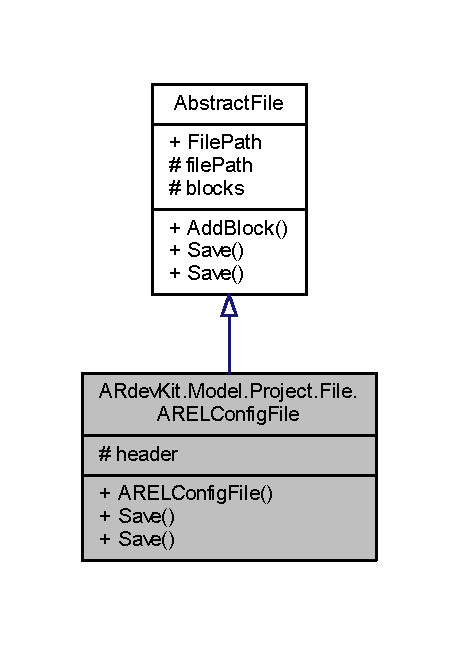
\includegraphics[width=220pt]{class_a_rdev_kit_1_1_model_1_1_project_1_1_file_1_1_a_r_e_l_config_file__inherit__graph}
\end{center}
\end{figure}


Collaboration diagram for A\-Rdev\-Kit.\-Model.\-Project.\-File.\-A\-R\-E\-L\-Config\-File\-:
\nopagebreak
\begin{figure}[H]
\begin{center}
\leavevmode
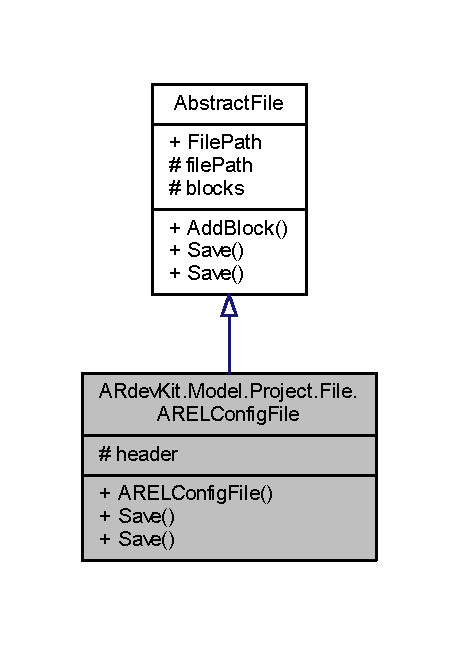
\includegraphics[width=220pt]{class_a_rdev_kit_1_1_model_1_1_project_1_1_file_1_1_a_r_e_l_config_file__coll__graph}
\end{center}
\end{figure}
\subsection*{Public Member Functions}
\begin{DoxyCompactItemize}
\item 
\hyperlink{class_a_rdev_kit_1_1_model_1_1_project_1_1_file_1_1_a_r_e_l_config_file_a740b9f9e195108cf418fff752545a88a}{A\-R\-E\-L\-Config\-File} (string \hyperlink{class_a_rdev_kit_1_1_model_1_1_project_1_1_file_1_1_a_r_e_l_config_file_a293887e7bfa91e75acfc21791106dc67}{header}, string project\-Path)
\begin{DoxyCompactList}\small\item\em Constructor. \end{DoxyCompactList}\item 
override void \hyperlink{class_a_rdev_kit_1_1_model_1_1_project_1_1_file_1_1_a_r_e_l_config_file_a65bf5e667cb70e7cb9ae9a735ebba97f}{Save} ()
\begin{DoxyCompactList}\small\item\em Saves the file to its \hyperlink{class_a_rdev_kit_1_1_model_1_1_project_1_1_file_1_1_abstract_file_ad879e3a81860da8b72f2d9f61a18ab3b}{file\-Path}. \end{DoxyCompactList}\item 
override void \hyperlink{class_a_rdev_kit_1_1_model_1_1_project_1_1_file_1_1_a_r_e_l_config_file_af0f2e70451d0dda0984dd186fcb6afde}{Save} (string project\-Path)
\begin{DoxyCompactList}\small\item\em Saves the file to the using the passed project\-Path. \end{DoxyCompactList}\end{DoxyCompactItemize}
\subsection*{Protected Attributes}
\begin{DoxyCompactItemize}
\item 
string \hyperlink{class_a_rdev_kit_1_1_model_1_1_project_1_1_file_1_1_a_r_e_l_config_file_a293887e7bfa91e75acfc21791106dc67}{header}
\begin{DoxyCompactList}\small\item\em The header. \end{DoxyCompactList}\end{DoxyCompactItemize}
\subsection*{Additional Inherited Members}


\subsection{Detailed Description}
An arel\-Config.\-xml. 

Imanuel, 17.\-01.\-2014. 

\subsection{Constructor \& Destructor Documentation}
\hypertarget{class_a_rdev_kit_1_1_model_1_1_project_1_1_file_1_1_a_r_e_l_config_file_a740b9f9e195108cf418fff752545a88a}{\index{A\-Rdev\-Kit\-::\-Model\-::\-Project\-::\-File\-::\-A\-R\-E\-L\-Config\-File@{A\-Rdev\-Kit\-::\-Model\-::\-Project\-::\-File\-::\-A\-R\-E\-L\-Config\-File}!A\-R\-E\-L\-Config\-File@{A\-R\-E\-L\-Config\-File}}
\index{A\-R\-E\-L\-Config\-File@{A\-R\-E\-L\-Config\-File}!ARdevKit::Model::Project::File::ARELConfigFile@{A\-Rdev\-Kit\-::\-Model\-::\-Project\-::\-File\-::\-A\-R\-E\-L\-Config\-File}}
\subsubsection[{A\-R\-E\-L\-Config\-File}]{\setlength{\rightskip}{0pt plus 5cm}A\-Rdev\-Kit.\-Model.\-Project.\-File.\-A\-R\-E\-L\-Config\-File.\-A\-R\-E\-L\-Config\-File (
\begin{DoxyParamCaption}
\item[{string}]{header, }
\item[{string}]{project\-Path}
\end{DoxyParamCaption}
)}}\label{class_a_rdev_kit_1_1_model_1_1_project_1_1_file_1_1_a_r_e_l_config_file_a740b9f9e195108cf418fff752545a88a}


Constructor. 


\begin{DoxyParams}{Parameters}
{\em header} & The header.\\
\hline
{\em project\-Path} & The project path.\\
\hline
\end{DoxyParams}


Imanuel, 15.\-01.\-2014. 

\subsection{Member Function Documentation}
\hypertarget{class_a_rdev_kit_1_1_model_1_1_project_1_1_file_1_1_a_r_e_l_config_file_a65bf5e667cb70e7cb9ae9a735ebba97f}{\index{A\-Rdev\-Kit\-::\-Model\-::\-Project\-::\-File\-::\-A\-R\-E\-L\-Config\-File@{A\-Rdev\-Kit\-::\-Model\-::\-Project\-::\-File\-::\-A\-R\-E\-L\-Config\-File}!Save@{Save}}
\index{Save@{Save}!ARdevKit::Model::Project::File::ARELConfigFile@{A\-Rdev\-Kit\-::\-Model\-::\-Project\-::\-File\-::\-A\-R\-E\-L\-Config\-File}}
\subsubsection[{Save}]{\setlength{\rightskip}{0pt plus 5cm}override void A\-Rdev\-Kit.\-Model.\-Project.\-File.\-A\-R\-E\-L\-Config\-File.\-Save (
\begin{DoxyParamCaption}
{}
\end{DoxyParamCaption}
)\hspace{0.3cm}{\ttfamily [virtual]}}}\label{class_a_rdev_kit_1_1_model_1_1_project_1_1_file_1_1_a_r_e_l_config_file_a65bf5e667cb70e7cb9ae9a735ebba97f}


Saves the file to its \hyperlink{class_a_rdev_kit_1_1_model_1_1_project_1_1_file_1_1_abstract_file_ad879e3a81860da8b72f2d9f61a18ab3b}{file\-Path}. 

Imanuel, 17.\-01.\-2014. 

Implements \hyperlink{class_a_rdev_kit_1_1_model_1_1_project_1_1_file_1_1_abstract_file_a095ebaeca96a6d285d9caff1ad726d5b}{A\-Rdev\-Kit.\-Model.\-Project.\-File.\-Abstract\-File}.

\hypertarget{class_a_rdev_kit_1_1_model_1_1_project_1_1_file_1_1_a_r_e_l_config_file_af0f2e70451d0dda0984dd186fcb6afde}{\index{A\-Rdev\-Kit\-::\-Model\-::\-Project\-::\-File\-::\-A\-R\-E\-L\-Config\-File@{A\-Rdev\-Kit\-::\-Model\-::\-Project\-::\-File\-::\-A\-R\-E\-L\-Config\-File}!Save@{Save}}
\index{Save@{Save}!ARdevKit::Model::Project::File::ARELConfigFile@{A\-Rdev\-Kit\-::\-Model\-::\-Project\-::\-File\-::\-A\-R\-E\-L\-Config\-File}}
\subsubsection[{Save}]{\setlength{\rightskip}{0pt plus 5cm}override void A\-Rdev\-Kit.\-Model.\-Project.\-File.\-A\-R\-E\-L\-Config\-File.\-Save (
\begin{DoxyParamCaption}
\item[{string}]{project\-Path}
\end{DoxyParamCaption}
)\hspace{0.3cm}{\ttfamily [virtual]}}}\label{class_a_rdev_kit_1_1_model_1_1_project_1_1_file_1_1_a_r_e_l_config_file_af0f2e70451d0dda0984dd186fcb6afde}


Saves the file to the using the passed project\-Path. 

Imanuel, 17.\-01.\-2014. 


\begin{DoxyParams}{Parameters}
{\em project\-Path} & The project path to write. \\
\hline
\end{DoxyParams}


Implements \hyperlink{class_a_rdev_kit_1_1_model_1_1_project_1_1_file_1_1_abstract_file_ae49c3262c59642e8f519d0655bbbbbab}{A\-Rdev\-Kit.\-Model.\-Project.\-File.\-Abstract\-File}.



\subsection{Member Data Documentation}
\hypertarget{class_a_rdev_kit_1_1_model_1_1_project_1_1_file_1_1_a_r_e_l_config_file_a293887e7bfa91e75acfc21791106dc67}{\index{A\-Rdev\-Kit\-::\-Model\-::\-Project\-::\-File\-::\-A\-R\-E\-L\-Config\-File@{A\-Rdev\-Kit\-::\-Model\-::\-Project\-::\-File\-::\-A\-R\-E\-L\-Config\-File}!header@{header}}
\index{header@{header}!ARdevKit::Model::Project::File::ARELConfigFile@{A\-Rdev\-Kit\-::\-Model\-::\-Project\-::\-File\-::\-A\-R\-E\-L\-Config\-File}}
\subsubsection[{header}]{\setlength{\rightskip}{0pt plus 5cm}string A\-Rdev\-Kit.\-Model.\-Project.\-File.\-A\-R\-E\-L\-Config\-File.\-header\hspace{0.3cm}{\ttfamily [protected]}}}\label{class_a_rdev_kit_1_1_model_1_1_project_1_1_file_1_1_a_r_e_l_config_file_a293887e7bfa91e75acfc21791106dc67}


The header. 


\hypertarget{class_a_rdev_kit_1_1_model_1_1_project_1_1_file_1_1_a_r_e_l_glue_file}{\section{A\-Rdev\-Kit.\-Model.\-Project.\-File.\-A\-R\-E\-L\-Glue\-File Class Reference}
\label{class_a_rdev_kit_1_1_model_1_1_project_1_1_file_1_1_a_r_e_l_glue_file}\index{A\-Rdev\-Kit.\-Model.\-Project.\-File.\-A\-R\-E\-L\-Glue\-File@{A\-Rdev\-Kit.\-Model.\-Project.\-File.\-A\-R\-E\-L\-Glue\-File}}
}


An arel\-Glue.\-js.  




Inheritance diagram for A\-Rdev\-Kit.\-Model.\-Project.\-File.\-A\-R\-E\-L\-Glue\-File\-:
\nopagebreak
\begin{figure}[H]
\begin{center}
\leavevmode
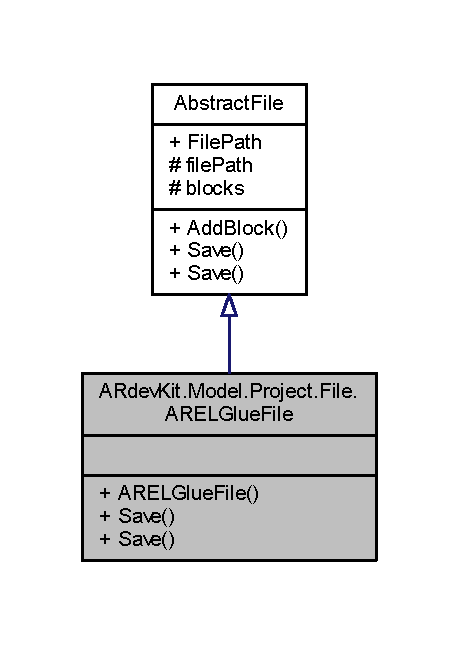
\includegraphics[width=220pt]{class_a_rdev_kit_1_1_model_1_1_project_1_1_file_1_1_a_r_e_l_glue_file__inherit__graph}
\end{center}
\end{figure}


Collaboration diagram for A\-Rdev\-Kit.\-Model.\-Project.\-File.\-A\-R\-E\-L\-Glue\-File\-:
\nopagebreak
\begin{figure}[H]
\begin{center}
\leavevmode
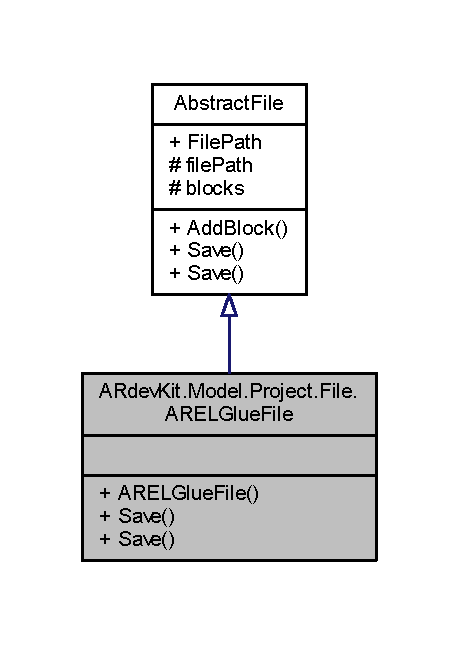
\includegraphics[width=220pt]{class_a_rdev_kit_1_1_model_1_1_project_1_1_file_1_1_a_r_e_l_glue_file__coll__graph}
\end{center}
\end{figure}
\subsection*{Public Member Functions}
\begin{DoxyCompactItemize}
\item 
\hyperlink{class_a_rdev_kit_1_1_model_1_1_project_1_1_file_1_1_a_r_e_l_glue_file_a944e3a92b64f3988dbd2e289fa3b2d36}{A\-R\-E\-L\-Glue\-File} (string project\-Path)
\begin{DoxyCompactList}\small\item\em Constructor. \end{DoxyCompactList}\item 
override void \hyperlink{class_a_rdev_kit_1_1_model_1_1_project_1_1_file_1_1_a_r_e_l_glue_file_af2a513e4dce9fe965fca00612335de10}{Save} ()
\begin{DoxyCompactList}\small\item\em Saves the file to its \hyperlink{class_a_rdev_kit_1_1_model_1_1_project_1_1_file_1_1_abstract_file_ad879e3a81860da8b72f2d9f61a18ab3b}{file\-Path}. \end{DoxyCompactList}\item 
override void \hyperlink{class_a_rdev_kit_1_1_model_1_1_project_1_1_file_1_1_a_r_e_l_glue_file_a82712a65053e760ba21b92fefe67baf3}{Save} (string project\-Path)
\begin{DoxyCompactList}\small\item\em Saves the file to the using the passed project\-Path. \end{DoxyCompactList}\end{DoxyCompactItemize}
\subsection*{Additional Inherited Members}


\subsection{Detailed Description}
An arel\-Glue.\-js. 

Imanuel, 17.\-01.\-2014. 

\subsection{Constructor \& Destructor Documentation}
\hypertarget{class_a_rdev_kit_1_1_model_1_1_project_1_1_file_1_1_a_r_e_l_glue_file_a944e3a92b64f3988dbd2e289fa3b2d36}{\index{A\-Rdev\-Kit\-::\-Model\-::\-Project\-::\-File\-::\-A\-R\-E\-L\-Glue\-File@{A\-Rdev\-Kit\-::\-Model\-::\-Project\-::\-File\-::\-A\-R\-E\-L\-Glue\-File}!A\-R\-E\-L\-Glue\-File@{A\-R\-E\-L\-Glue\-File}}
\index{A\-R\-E\-L\-Glue\-File@{A\-R\-E\-L\-Glue\-File}!ARdevKit::Model::Project::File::ARELGlueFile@{A\-Rdev\-Kit\-::\-Model\-::\-Project\-::\-File\-::\-A\-R\-E\-L\-Glue\-File}}
\subsubsection[{A\-R\-E\-L\-Glue\-File}]{\setlength{\rightskip}{0pt plus 5cm}A\-Rdev\-Kit.\-Model.\-Project.\-File.\-A\-R\-E\-L\-Glue\-File.\-A\-R\-E\-L\-Glue\-File (
\begin{DoxyParamCaption}
\item[{string}]{project\-Path}
\end{DoxyParamCaption}
)}}\label{class_a_rdev_kit_1_1_model_1_1_project_1_1_file_1_1_a_r_e_l_glue_file_a944e3a92b64f3988dbd2e289fa3b2d36}


Constructor. 

Imanuel, 17.\-01.\-2014. 


\begin{DoxyParams}{Parameters}
{\em project\-Path} & Full pathname of the project file. \\
\hline
\end{DoxyParams}


\subsection{Member Function Documentation}
\hypertarget{class_a_rdev_kit_1_1_model_1_1_project_1_1_file_1_1_a_r_e_l_glue_file_af2a513e4dce9fe965fca00612335de10}{\index{A\-Rdev\-Kit\-::\-Model\-::\-Project\-::\-File\-::\-A\-R\-E\-L\-Glue\-File@{A\-Rdev\-Kit\-::\-Model\-::\-Project\-::\-File\-::\-A\-R\-E\-L\-Glue\-File}!Save@{Save}}
\index{Save@{Save}!ARdevKit::Model::Project::File::ARELGlueFile@{A\-Rdev\-Kit\-::\-Model\-::\-Project\-::\-File\-::\-A\-R\-E\-L\-Glue\-File}}
\subsubsection[{Save}]{\setlength{\rightskip}{0pt plus 5cm}override void A\-Rdev\-Kit.\-Model.\-Project.\-File.\-A\-R\-E\-L\-Glue\-File.\-Save (
\begin{DoxyParamCaption}
{}
\end{DoxyParamCaption}
)\hspace{0.3cm}{\ttfamily [virtual]}}}\label{class_a_rdev_kit_1_1_model_1_1_project_1_1_file_1_1_a_r_e_l_glue_file_af2a513e4dce9fe965fca00612335de10}


Saves the file to its \hyperlink{class_a_rdev_kit_1_1_model_1_1_project_1_1_file_1_1_abstract_file_ad879e3a81860da8b72f2d9f61a18ab3b}{file\-Path}. 

Imanuel, 17.\-01.\-2014. 

Implements \hyperlink{class_a_rdev_kit_1_1_model_1_1_project_1_1_file_1_1_abstract_file_a095ebaeca96a6d285d9caff1ad726d5b}{A\-Rdev\-Kit.\-Model.\-Project.\-File.\-Abstract\-File}.

\hypertarget{class_a_rdev_kit_1_1_model_1_1_project_1_1_file_1_1_a_r_e_l_glue_file_a82712a65053e760ba21b92fefe67baf3}{\index{A\-Rdev\-Kit\-::\-Model\-::\-Project\-::\-File\-::\-A\-R\-E\-L\-Glue\-File@{A\-Rdev\-Kit\-::\-Model\-::\-Project\-::\-File\-::\-A\-R\-E\-L\-Glue\-File}!Save@{Save}}
\index{Save@{Save}!ARdevKit::Model::Project::File::ARELGlueFile@{A\-Rdev\-Kit\-::\-Model\-::\-Project\-::\-File\-::\-A\-R\-E\-L\-Glue\-File}}
\subsubsection[{Save}]{\setlength{\rightskip}{0pt plus 5cm}override void A\-Rdev\-Kit.\-Model.\-Project.\-File.\-A\-R\-E\-L\-Glue\-File.\-Save (
\begin{DoxyParamCaption}
\item[{string}]{project\-Path}
\end{DoxyParamCaption}
)\hspace{0.3cm}{\ttfamily [virtual]}}}\label{class_a_rdev_kit_1_1_model_1_1_project_1_1_file_1_1_a_r_e_l_glue_file_a82712a65053e760ba21b92fefe67baf3}


Saves the file to the using the passed project\-Path. 

Imanuel, 17.\-01.\-2014. 


\begin{DoxyParams}{Parameters}
{\em project\-Path} & The project path to write. \\
\hline
\end{DoxyParams}


Implements \hyperlink{class_a_rdev_kit_1_1_model_1_1_project_1_1_file_1_1_abstract_file_ae49c3262c59642e8f519d0655bbbbbab}{A\-Rdev\-Kit.\-Model.\-Project.\-File.\-Abstract\-File}.


\hypertarget{class_a_rdev_kit_1_1_model_1_1_project_1_1_file_1_1_a_r_e_l_project_file}{\section{A\-Rdev\-Kit.\-Model.\-Project.\-File.\-A\-R\-E\-L\-Project\-File Class Reference}
\label{class_a_rdev_kit_1_1_model_1_1_project_1_1_file_1_1_a_r_e_l_project_file}\index{A\-Rdev\-Kit.\-Model.\-Project.\-File.\-A\-R\-E\-L\-Project\-File@{A\-Rdev\-Kit.\-Model.\-Project.\-File.\-A\-R\-E\-L\-Project\-File}}
}


A arel\mbox{[}project\-Name\mbox{]}.html.  




Inheritance diagram for A\-Rdev\-Kit.\-Model.\-Project.\-File.\-A\-R\-E\-L\-Project\-File\-:
\nopagebreak
\begin{figure}[H]
\begin{center}
\leavevmode
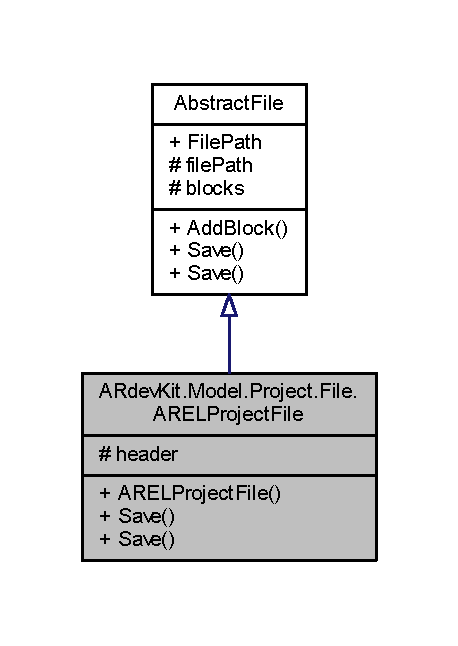
\includegraphics[width=220pt]{class_a_rdev_kit_1_1_model_1_1_project_1_1_file_1_1_a_r_e_l_project_file__inherit__graph}
\end{center}
\end{figure}


Collaboration diagram for A\-Rdev\-Kit.\-Model.\-Project.\-File.\-A\-R\-E\-L\-Project\-File\-:
\nopagebreak
\begin{figure}[H]
\begin{center}
\leavevmode
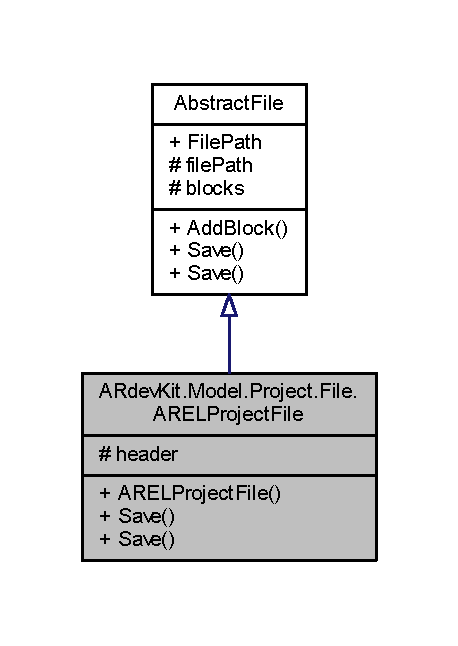
\includegraphics[width=220pt]{class_a_rdev_kit_1_1_model_1_1_project_1_1_file_1_1_a_r_e_l_project_file__coll__graph}
\end{center}
\end{figure}
\subsection*{Public Member Functions}
\begin{DoxyCompactItemize}
\item 
\hyperlink{class_a_rdev_kit_1_1_model_1_1_project_1_1_file_1_1_a_r_e_l_project_file_a9b94a89662d8c29e26f6fcb98d40e332}{A\-R\-E\-L\-Project\-File} (string \hyperlink{class_a_rdev_kit_1_1_model_1_1_project_1_1_file_1_1_a_r_e_l_project_file_aa23070e2b62c07d4c41a5555ab673326}{header}, string \hyperlink{class_a_rdev_kit_1_1_model_1_1_project_1_1_file_1_1_abstract_file_ad879e3a81860da8b72f2d9f61a18ab3b}{file\-Path})
\begin{DoxyCompactList}\small\item\em Constructor. \end{DoxyCompactList}\item 
override void \hyperlink{class_a_rdev_kit_1_1_model_1_1_project_1_1_file_1_1_a_r_e_l_project_file_a021507cbd83b07773ffc1caf0645ca49}{Save} ()
\begin{DoxyCompactList}\small\item\em Saves the file to its \hyperlink{class_a_rdev_kit_1_1_model_1_1_project_1_1_file_1_1_abstract_file_ad879e3a81860da8b72f2d9f61a18ab3b}{file\-Path}. \end{DoxyCompactList}\item 
override void \hyperlink{class_a_rdev_kit_1_1_model_1_1_project_1_1_file_1_1_a_r_e_l_project_file_aa187897624d6d836b3a76331069d5bee}{Save} (string \hyperlink{class_a_rdev_kit_1_1_model_1_1_project_1_1_file_1_1_abstract_file_ad879e3a81860da8b72f2d9f61a18ab3b}{file\-Path})
\begin{DoxyCompactList}\small\item\em Saves the file to the using the passed project\-Path. \end{DoxyCompactList}\end{DoxyCompactItemize}
\subsection*{Protected Attributes}
\begin{DoxyCompactItemize}
\item 
string \hyperlink{class_a_rdev_kit_1_1_model_1_1_project_1_1_file_1_1_a_r_e_l_project_file_aa23070e2b62c07d4c41a5555ab673326}{header}
\begin{DoxyCompactList}\small\item\em The header. \end{DoxyCompactList}\end{DoxyCompactItemize}
\subsection*{Additional Inherited Members}


\subsection{Detailed Description}
A arel\mbox{[}project\-Name\mbox{]}.html. 

Imanuel, 15.\-01.\-2014. 

\subsection{Constructor \& Destructor Documentation}
\hypertarget{class_a_rdev_kit_1_1_model_1_1_project_1_1_file_1_1_a_r_e_l_project_file_a9b94a89662d8c29e26f6fcb98d40e332}{\index{A\-Rdev\-Kit\-::\-Model\-::\-Project\-::\-File\-::\-A\-R\-E\-L\-Project\-File@{A\-Rdev\-Kit\-::\-Model\-::\-Project\-::\-File\-::\-A\-R\-E\-L\-Project\-File}!A\-R\-E\-L\-Project\-File@{A\-R\-E\-L\-Project\-File}}
\index{A\-R\-E\-L\-Project\-File@{A\-R\-E\-L\-Project\-File}!ARdevKit::Model::Project::File::ARELProjectFile@{A\-Rdev\-Kit\-::\-Model\-::\-Project\-::\-File\-::\-A\-R\-E\-L\-Project\-File}}
\subsubsection[{A\-R\-E\-L\-Project\-File}]{\setlength{\rightskip}{0pt plus 5cm}A\-Rdev\-Kit.\-Model.\-Project.\-File.\-A\-R\-E\-L\-Project\-File.\-A\-R\-E\-L\-Project\-File (
\begin{DoxyParamCaption}
\item[{string}]{header, }
\item[{string}]{file\-Path}
\end{DoxyParamCaption}
)}}\label{class_a_rdev_kit_1_1_model_1_1_project_1_1_file_1_1_a_r_e_l_project_file_a9b94a89662d8c29e26f6fcb98d40e332}


Constructor. 


\begin{DoxyParams}{Parameters}
{\em header} & The header.\\
\hline
{\em file\-Path} & The file path.\\
\hline
\end{DoxyParams}


Imanuel, 15.\-01.\-2014. 

\subsection{Member Function Documentation}
\hypertarget{class_a_rdev_kit_1_1_model_1_1_project_1_1_file_1_1_a_r_e_l_project_file_a021507cbd83b07773ffc1caf0645ca49}{\index{A\-Rdev\-Kit\-::\-Model\-::\-Project\-::\-File\-::\-A\-R\-E\-L\-Project\-File@{A\-Rdev\-Kit\-::\-Model\-::\-Project\-::\-File\-::\-A\-R\-E\-L\-Project\-File}!Save@{Save}}
\index{Save@{Save}!ARdevKit::Model::Project::File::ARELProjectFile@{A\-Rdev\-Kit\-::\-Model\-::\-Project\-::\-File\-::\-A\-R\-E\-L\-Project\-File}}
\subsubsection[{Save}]{\setlength{\rightskip}{0pt plus 5cm}override void A\-Rdev\-Kit.\-Model.\-Project.\-File.\-A\-R\-E\-L\-Project\-File.\-Save (
\begin{DoxyParamCaption}
{}
\end{DoxyParamCaption}
)\hspace{0.3cm}{\ttfamily [virtual]}}}\label{class_a_rdev_kit_1_1_model_1_1_project_1_1_file_1_1_a_r_e_l_project_file_a021507cbd83b07773ffc1caf0645ca49}


Saves the file to its \hyperlink{class_a_rdev_kit_1_1_model_1_1_project_1_1_file_1_1_abstract_file_ad879e3a81860da8b72f2d9f61a18ab3b}{file\-Path}. 

Imanuel, 17.\-01.\-2014. 

Implements \hyperlink{class_a_rdev_kit_1_1_model_1_1_project_1_1_file_1_1_abstract_file_a095ebaeca96a6d285d9caff1ad726d5b}{A\-Rdev\-Kit.\-Model.\-Project.\-File.\-Abstract\-File}.

\hypertarget{class_a_rdev_kit_1_1_model_1_1_project_1_1_file_1_1_a_r_e_l_project_file_aa187897624d6d836b3a76331069d5bee}{\index{A\-Rdev\-Kit\-::\-Model\-::\-Project\-::\-File\-::\-A\-R\-E\-L\-Project\-File@{A\-Rdev\-Kit\-::\-Model\-::\-Project\-::\-File\-::\-A\-R\-E\-L\-Project\-File}!Save@{Save}}
\index{Save@{Save}!ARdevKit::Model::Project::File::ARELProjectFile@{A\-Rdev\-Kit\-::\-Model\-::\-Project\-::\-File\-::\-A\-R\-E\-L\-Project\-File}}
\subsubsection[{Save}]{\setlength{\rightskip}{0pt plus 5cm}override void A\-Rdev\-Kit.\-Model.\-Project.\-File.\-A\-R\-E\-L\-Project\-File.\-Save (
\begin{DoxyParamCaption}
\item[{string}]{file\-Path}
\end{DoxyParamCaption}
)\hspace{0.3cm}{\ttfamily [virtual]}}}\label{class_a_rdev_kit_1_1_model_1_1_project_1_1_file_1_1_a_r_e_l_project_file_aa187897624d6d836b3a76331069d5bee}


Saves the file to the using the passed project\-Path. 

Imanuel, 17.\-01.\-2014. 


\begin{DoxyParams}{Parameters}
{\em file\-Path} & The project path to write. \\
\hline
\end{DoxyParams}


Implements \hyperlink{class_a_rdev_kit_1_1_model_1_1_project_1_1_file_1_1_abstract_file_ae49c3262c59642e8f519d0655bbbbbab}{A\-Rdev\-Kit.\-Model.\-Project.\-File.\-Abstract\-File}.



\subsection{Member Data Documentation}
\hypertarget{class_a_rdev_kit_1_1_model_1_1_project_1_1_file_1_1_a_r_e_l_project_file_aa23070e2b62c07d4c41a5555ab673326}{\index{A\-Rdev\-Kit\-::\-Model\-::\-Project\-::\-File\-::\-A\-R\-E\-L\-Project\-File@{A\-Rdev\-Kit\-::\-Model\-::\-Project\-::\-File\-::\-A\-R\-E\-L\-Project\-File}!header@{header}}
\index{header@{header}!ARdevKit::Model::Project::File::ARELProjectFile@{A\-Rdev\-Kit\-::\-Model\-::\-Project\-::\-File\-::\-A\-R\-E\-L\-Project\-File}}
\subsubsection[{header}]{\setlength{\rightskip}{0pt plus 5cm}string A\-Rdev\-Kit.\-Model.\-Project.\-File.\-A\-R\-E\-L\-Project\-File.\-header\hspace{0.3cm}{\ttfamily [protected]}}}\label{class_a_rdev_kit_1_1_model_1_1_project_1_1_file_1_1_a_r_e_l_project_file_aa23070e2b62c07d4c41a5555ab673326}


The header. 


\hypertarget{class_a_rdev_kit_1_1_model_1_1_project_1_1_file_1_1_block_marker}{\section{A\-Rdev\-Kit.\-Model.\-Project.\-File.\-Block\-Marker Class Reference}
\label{class_a_rdev_kit_1_1_model_1_1_project_1_1_file_1_1_block_marker}\index{A\-Rdev\-Kit.\-Model.\-Project.\-File.\-Block\-Marker@{A\-Rdev\-Kit.\-Model.\-Project.\-File.\-Block\-Marker}}
}


A \hyperlink{class_a_rdev_kit_1_1_model_1_1_project_1_1_file_1_1_block_marker}{Block\-Marker} marks an \hyperlink{class_a_rdev_kit_1_1_model_1_1_project_1_1_file_1_1_abstract_block}{Abstract\-Block}. It has a \hyperlink{class_a_rdev_kit_1_1_model_1_1_project_1_1_file_1_1_block_marker_a7764ae600714a07a74b8ddf55f1a59d5}{Start} string and an \hyperlink{class_a_rdev_kit_1_1_model_1_1_project_1_1_file_1_1_block_marker_a3672477b3c409c07c7189a57fbd004c4}{End} string and can be open or closed.  




Inheritance diagram for A\-Rdev\-Kit.\-Model.\-Project.\-File.\-Block\-Marker\-:
\nopagebreak
\begin{figure}[H]
\begin{center}
\leavevmode
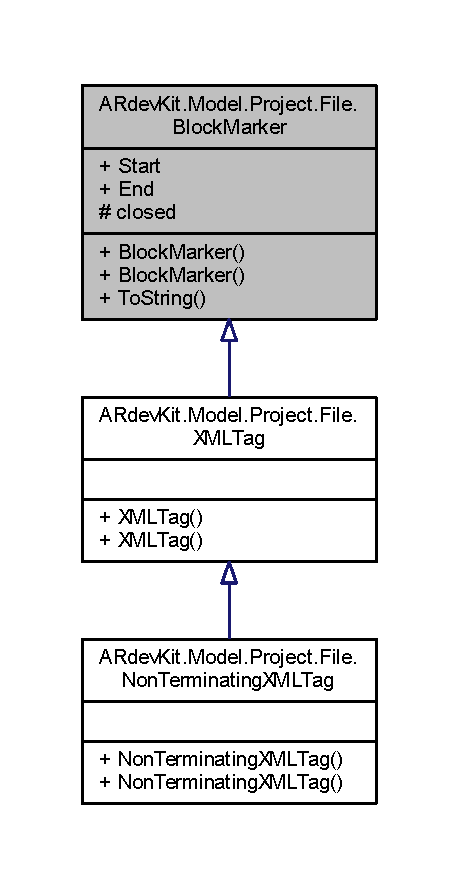
\includegraphics[width=220pt]{class_a_rdev_kit_1_1_model_1_1_project_1_1_file_1_1_block_marker__inherit__graph}
\end{center}
\end{figure}


Collaboration diagram for A\-Rdev\-Kit.\-Model.\-Project.\-File.\-Block\-Marker\-:
\nopagebreak
\begin{figure}[H]
\begin{center}
\leavevmode
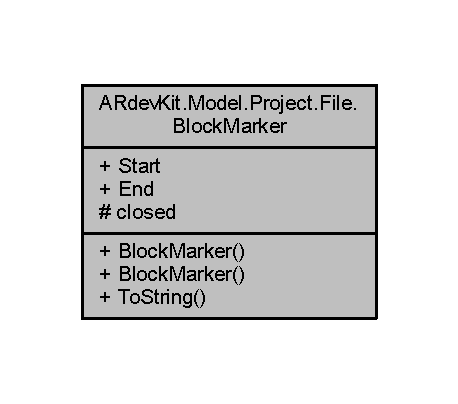
\includegraphics[width=220pt]{class_a_rdev_kit_1_1_model_1_1_project_1_1_file_1_1_block_marker__coll__graph}
\end{center}
\end{figure}
\subsection*{Public Member Functions}
\begin{DoxyCompactItemize}
\item 
\hyperlink{class_a_rdev_kit_1_1_model_1_1_project_1_1_file_1_1_block_marker_a148e8916c49f13adff386c50d0b45738}{Block\-Marker} ()
\begin{DoxyCompactList}\small\item\em Default constructor. \end{DoxyCompactList}\item 
\hyperlink{class_a_rdev_kit_1_1_model_1_1_project_1_1_file_1_1_block_marker_aa9b3cdf82da639e651b73eff5ec7938f}{Block\-Marker} (string start, string end)
\begin{DoxyCompactList}\small\item\em Constructor. \end{DoxyCompactList}\item 
override string \hyperlink{class_a_rdev_kit_1_1_model_1_1_project_1_1_file_1_1_block_marker_a5334b9dcd41a81ccac65d7c98062c43a}{To\-String} ()
\begin{DoxyCompactList}\small\item\em Returns the start and end part alternating. Beginning with the start part on first call.\end{DoxyCompactList}\end{DoxyCompactItemize}
\subsection*{Protected Attributes}
\begin{DoxyCompactItemize}
\item 
bool \hyperlink{class_a_rdev_kit_1_1_model_1_1_project_1_1_file_1_1_block_marker_add534689f3e6af2448ee6194305ceafc}{closed} = true
\begin{DoxyCompactList}\small\item\em true if closed. \end{DoxyCompactList}\end{DoxyCompactItemize}
\subsection*{Properties}
\begin{DoxyCompactItemize}
\item 
string \hyperlink{class_a_rdev_kit_1_1_model_1_1_project_1_1_file_1_1_block_marker_a7764ae600714a07a74b8ddf55f1a59d5}{Start}\hspace{0.3cm}{\ttfamily  \mbox{[}get, set\mbox{]}}
\begin{DoxyCompactList}\small\item\em Gets or sets the start. \end{DoxyCompactList}\item 
string \hyperlink{class_a_rdev_kit_1_1_model_1_1_project_1_1_file_1_1_block_marker_a3672477b3c409c07c7189a57fbd004c4}{End}\hspace{0.3cm}{\ttfamily  \mbox{[}get, set\mbox{]}}
\begin{DoxyCompactList}\small\item\em Gets or sets the end. \end{DoxyCompactList}\end{DoxyCompactItemize}


\subsection{Detailed Description}
A \hyperlink{class_a_rdev_kit_1_1_model_1_1_project_1_1_file_1_1_block_marker}{Block\-Marker} marks an \hyperlink{class_a_rdev_kit_1_1_model_1_1_project_1_1_file_1_1_abstract_block}{Abstract\-Block}. It has a \hyperlink{class_a_rdev_kit_1_1_model_1_1_project_1_1_file_1_1_block_marker_a7764ae600714a07a74b8ddf55f1a59d5}{Start} string and an \hyperlink{class_a_rdev_kit_1_1_model_1_1_project_1_1_file_1_1_block_marker_a3672477b3c409c07c7189a57fbd004c4}{End} string and can be open or closed. 

Imanuel, 17.\-01.\-2014. 

\subsection{Constructor \& Destructor Documentation}
\hypertarget{class_a_rdev_kit_1_1_model_1_1_project_1_1_file_1_1_block_marker_a148e8916c49f13adff386c50d0b45738}{\index{A\-Rdev\-Kit\-::\-Model\-::\-Project\-::\-File\-::\-Block\-Marker@{A\-Rdev\-Kit\-::\-Model\-::\-Project\-::\-File\-::\-Block\-Marker}!Block\-Marker@{Block\-Marker}}
\index{Block\-Marker@{Block\-Marker}!ARdevKit::Model::Project::File::BlockMarker@{A\-Rdev\-Kit\-::\-Model\-::\-Project\-::\-File\-::\-Block\-Marker}}
\subsubsection[{Block\-Marker}]{\setlength{\rightskip}{0pt plus 5cm}A\-Rdev\-Kit.\-Model.\-Project.\-File.\-Block\-Marker.\-Block\-Marker (
\begin{DoxyParamCaption}
{}
\end{DoxyParamCaption}
)}}\label{class_a_rdev_kit_1_1_model_1_1_project_1_1_file_1_1_block_marker_a148e8916c49f13adff386c50d0b45738}


Default constructor. 

Imanuel, 17.\-01.\-2014. \hypertarget{class_a_rdev_kit_1_1_model_1_1_project_1_1_file_1_1_block_marker_aa9b3cdf82da639e651b73eff5ec7938f}{\index{A\-Rdev\-Kit\-::\-Model\-::\-Project\-::\-File\-::\-Block\-Marker@{A\-Rdev\-Kit\-::\-Model\-::\-Project\-::\-File\-::\-Block\-Marker}!Block\-Marker@{Block\-Marker}}
\index{Block\-Marker@{Block\-Marker}!ARdevKit::Model::Project::File::BlockMarker@{A\-Rdev\-Kit\-::\-Model\-::\-Project\-::\-File\-::\-Block\-Marker}}
\subsubsection[{Block\-Marker}]{\setlength{\rightskip}{0pt plus 5cm}A\-Rdev\-Kit.\-Model.\-Project.\-File.\-Block\-Marker.\-Block\-Marker (
\begin{DoxyParamCaption}
\item[{string}]{start, }
\item[{string}]{end}
\end{DoxyParamCaption}
)}}\label{class_a_rdev_kit_1_1_model_1_1_project_1_1_file_1_1_block_marker_aa9b3cdf82da639e651b73eff5ec7938f}


Constructor. 

Imanuel, 17.\-01.\-2014. 


\begin{DoxyParams}{Parameters}
{\em start} & The start. \\
\hline
{\em end} & The end. \\
\hline
\end{DoxyParams}


\subsection{Member Function Documentation}
\hypertarget{class_a_rdev_kit_1_1_model_1_1_project_1_1_file_1_1_block_marker_a5334b9dcd41a81ccac65d7c98062c43a}{\index{A\-Rdev\-Kit\-::\-Model\-::\-Project\-::\-File\-::\-Block\-Marker@{A\-Rdev\-Kit\-::\-Model\-::\-Project\-::\-File\-::\-Block\-Marker}!To\-String@{To\-String}}
\index{To\-String@{To\-String}!ARdevKit::Model::Project::File::BlockMarker@{A\-Rdev\-Kit\-::\-Model\-::\-Project\-::\-File\-::\-Block\-Marker}}
\subsubsection[{To\-String}]{\setlength{\rightskip}{0pt plus 5cm}override string A\-Rdev\-Kit.\-Model.\-Project.\-File.\-Block\-Marker.\-To\-String (
\begin{DoxyParamCaption}
{}
\end{DoxyParamCaption}
)}}\label{class_a_rdev_kit_1_1_model_1_1_project_1_1_file_1_1_block_marker_a5334b9dcd41a81ccac65d7c98062c43a}


Returns the start and end part alternating. Beginning with the start part on first call.

Imanuel, 15.\-01.\-2014. 

\begin{DoxyReturn}{Returns}
Eine Zeichenfolge, die das aktuelle Objekt darstellt. 
\end{DoxyReturn}


\subsection{Member Data Documentation}
\hypertarget{class_a_rdev_kit_1_1_model_1_1_project_1_1_file_1_1_block_marker_add534689f3e6af2448ee6194305ceafc}{\index{A\-Rdev\-Kit\-::\-Model\-::\-Project\-::\-File\-::\-Block\-Marker@{A\-Rdev\-Kit\-::\-Model\-::\-Project\-::\-File\-::\-Block\-Marker}!closed@{closed}}
\index{closed@{closed}!ARdevKit::Model::Project::File::BlockMarker@{A\-Rdev\-Kit\-::\-Model\-::\-Project\-::\-File\-::\-Block\-Marker}}
\subsubsection[{closed}]{\setlength{\rightskip}{0pt plus 5cm}bool A\-Rdev\-Kit.\-Model.\-Project.\-File.\-Block\-Marker.\-closed = true\hspace{0.3cm}{\ttfamily [protected]}}}\label{class_a_rdev_kit_1_1_model_1_1_project_1_1_file_1_1_block_marker_add534689f3e6af2448ee6194305ceafc}


true if closed. 



\subsection{Property Documentation}
\hypertarget{class_a_rdev_kit_1_1_model_1_1_project_1_1_file_1_1_block_marker_a3672477b3c409c07c7189a57fbd004c4}{\index{A\-Rdev\-Kit\-::\-Model\-::\-Project\-::\-File\-::\-Block\-Marker@{A\-Rdev\-Kit\-::\-Model\-::\-Project\-::\-File\-::\-Block\-Marker}!End@{End}}
\index{End@{End}!ARdevKit::Model::Project::File::BlockMarker@{A\-Rdev\-Kit\-::\-Model\-::\-Project\-::\-File\-::\-Block\-Marker}}
\subsubsection[{End}]{\setlength{\rightskip}{0pt plus 5cm}string A\-Rdev\-Kit.\-Model.\-Project.\-File.\-Block\-Marker.\-End\hspace{0.3cm}{\ttfamily [get]}, {\ttfamily [set]}}}\label{class_a_rdev_kit_1_1_model_1_1_project_1_1_file_1_1_block_marker_a3672477b3c409c07c7189a57fbd004c4}


Gets or sets the end. 

The end. \hypertarget{class_a_rdev_kit_1_1_model_1_1_project_1_1_file_1_1_block_marker_a7764ae600714a07a74b8ddf55f1a59d5}{\index{A\-Rdev\-Kit\-::\-Model\-::\-Project\-::\-File\-::\-Block\-Marker@{A\-Rdev\-Kit\-::\-Model\-::\-Project\-::\-File\-::\-Block\-Marker}!Start@{Start}}
\index{Start@{Start}!ARdevKit::Model::Project::File::BlockMarker@{A\-Rdev\-Kit\-::\-Model\-::\-Project\-::\-File\-::\-Block\-Marker}}
\subsubsection[{Start}]{\setlength{\rightskip}{0pt plus 5cm}string A\-Rdev\-Kit.\-Model.\-Project.\-File.\-Block\-Marker.\-Start\hspace{0.3cm}{\ttfamily [get]}, {\ttfamily [set]}}}\label{class_a_rdev_kit_1_1_model_1_1_project_1_1_file_1_1_block_marker_a7764ae600714a07a74b8ddf55f1a59d5}


Gets or sets the start. 

The start. 
\hypertarget{class_a_rdev_kit_1_1_model_1_1_project_1_1_chart}{\section{A\-Rdev\-Kit.\-Model.\-Project.\-Chart Class Reference}
\label{class_a_rdev_kit_1_1_model_1_1_project_1_1_chart}\index{A\-Rdev\-Kit.\-Model.\-Project.\-Chart@{A\-Rdev\-Kit.\-Model.\-Project.\-Chart}}
}


Describes a \hyperlink{class_a_rdev_kit_1_1_model_1_1_project_1_1_chart}{Chart} with its Colors and Optimal\-Values. It is a \hyperlink{class_a_rdev_kit_1_1_model_1_1_project_1_1_chart}{Chart}.  




Inheritance diagram for A\-Rdev\-Kit.\-Model.\-Project.\-Chart\-:
\nopagebreak
\begin{figure}[H]
\begin{center}
\leavevmode
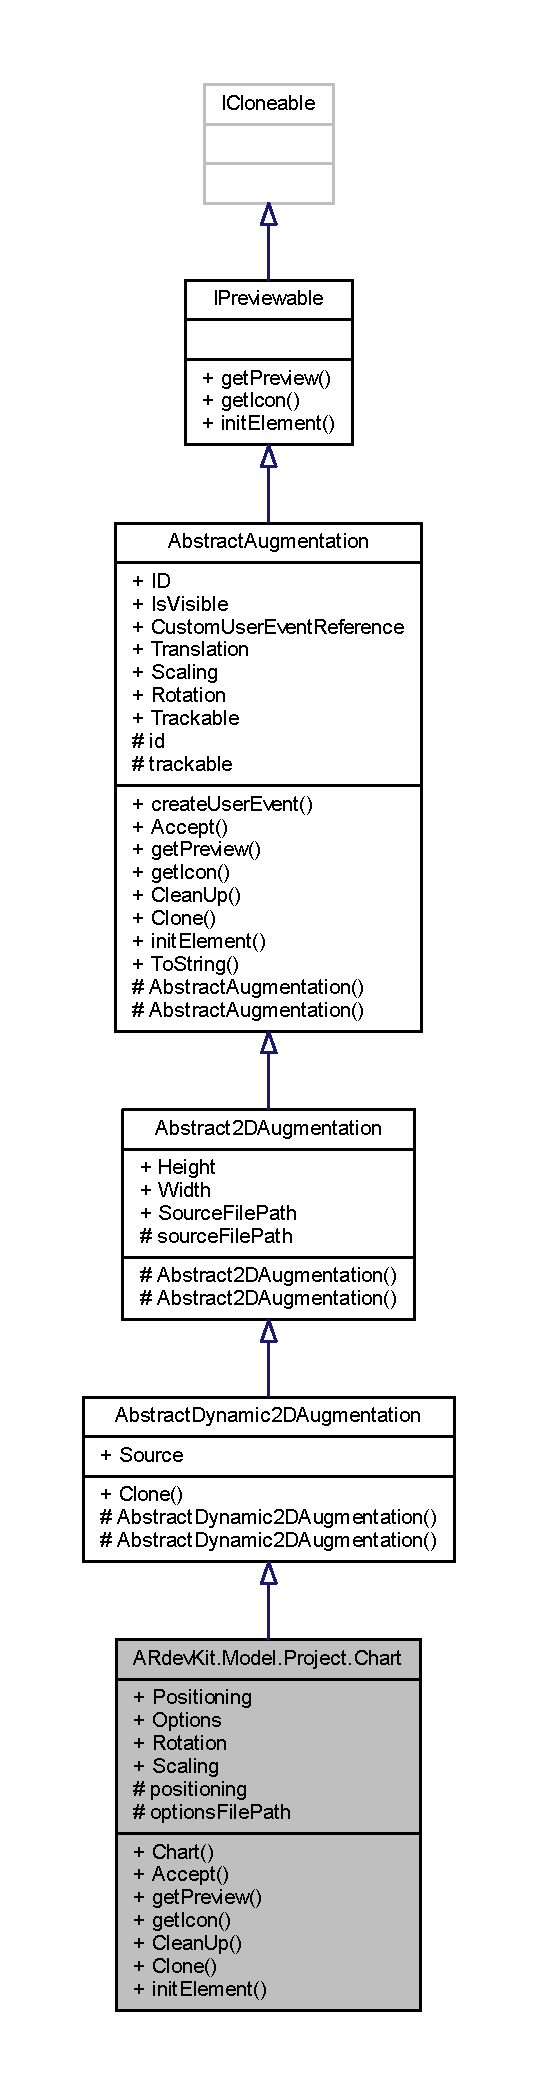
\includegraphics[height=550pt]{class_a_rdev_kit_1_1_model_1_1_project_1_1_chart__inherit__graph}
\end{center}
\end{figure}


Collaboration diagram for A\-Rdev\-Kit.\-Model.\-Project.\-Chart\-:
\nopagebreak
\begin{figure}[H]
\begin{center}
\leavevmode
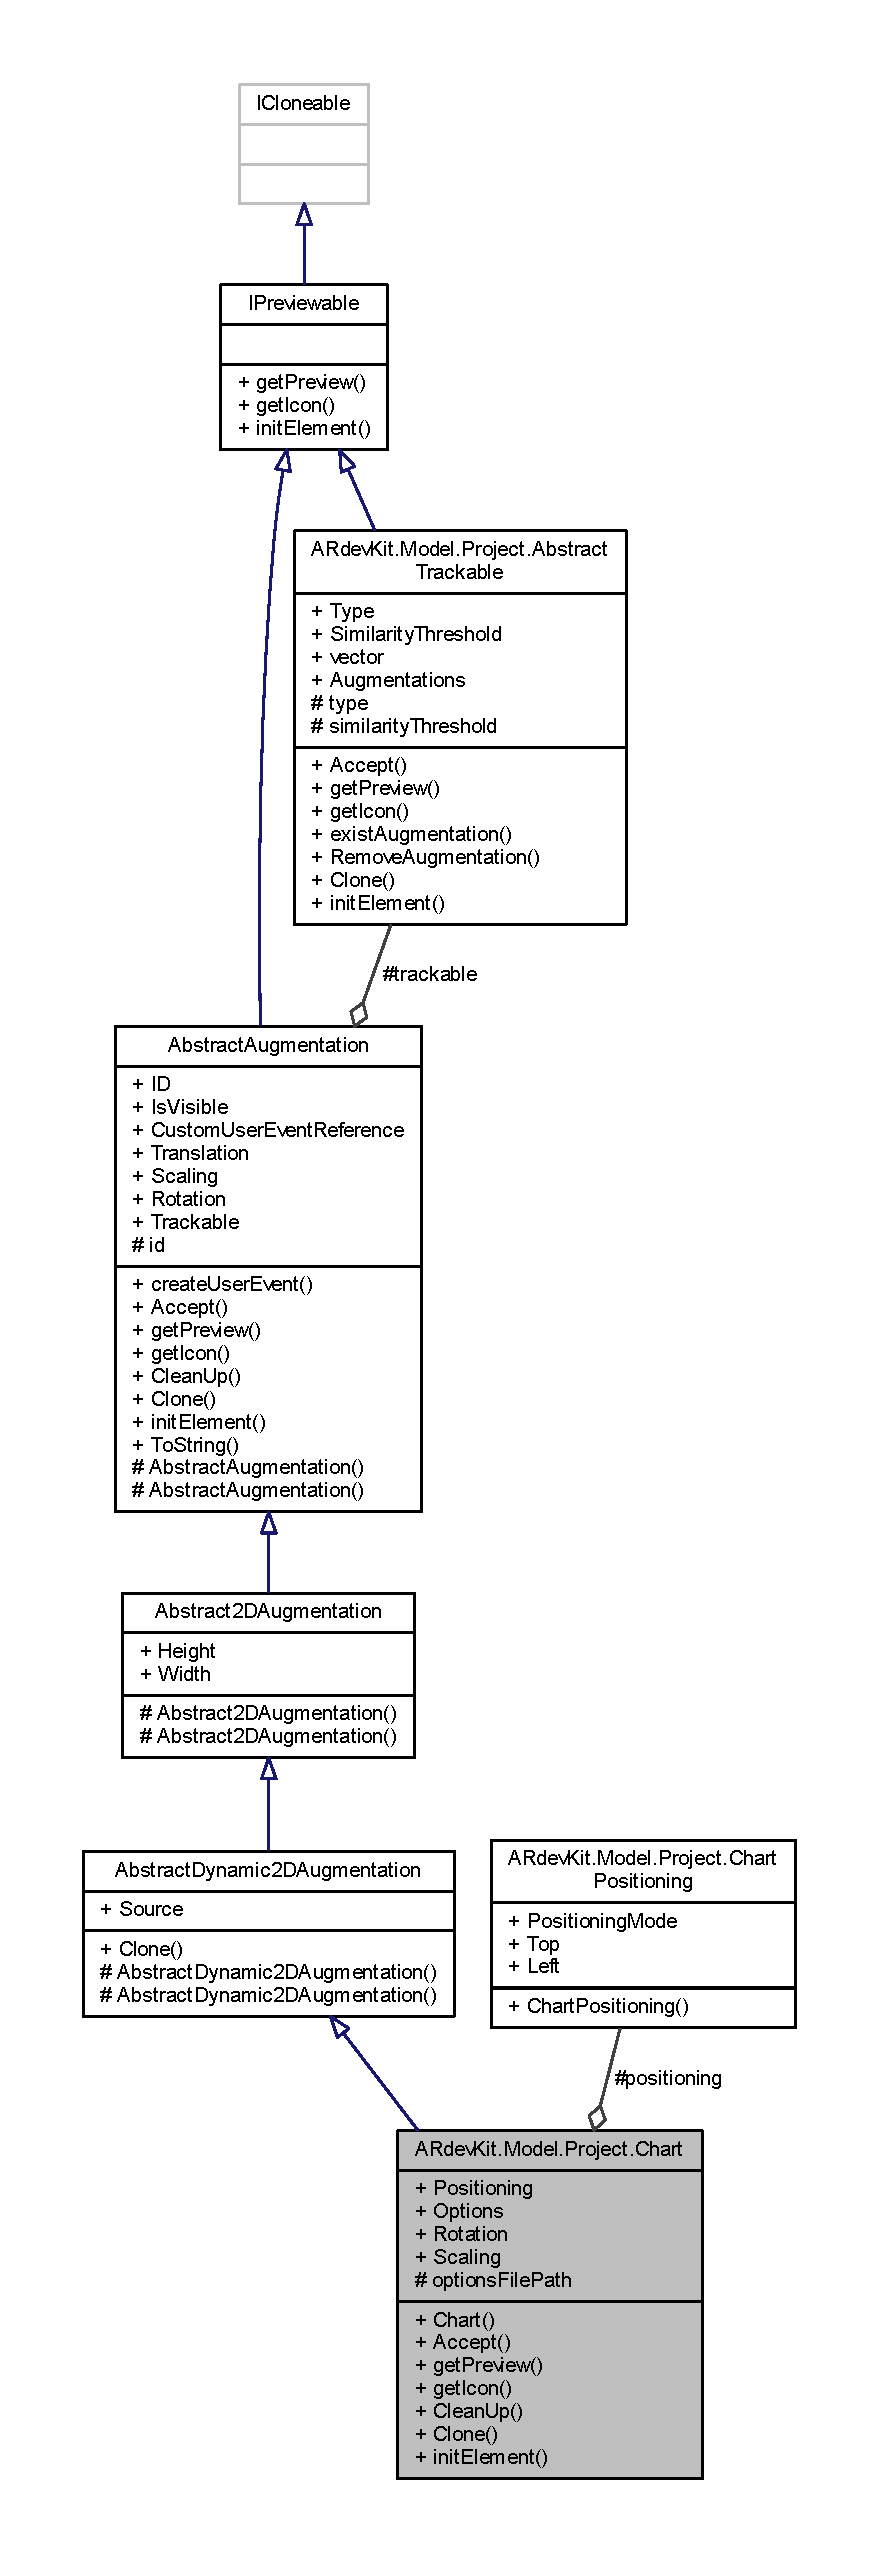
\includegraphics[height=550pt]{class_a_rdev_kit_1_1_model_1_1_project_1_1_chart__coll__graph}
\end{center}
\end{figure}
\subsection*{Public Member Functions}
\begin{DoxyCompactItemize}
\item 
\hyperlink{class_a_rdev_kit_1_1_model_1_1_project_1_1_chart_adc15fc2ed54bf85d32868514e94afb28}{Chart} ()
\begin{DoxyCompactList}\small\item\em Default constructor. \end{DoxyCompactList}\item 
override void \hyperlink{class_a_rdev_kit_1_1_model_1_1_project_1_1_chart_a45ba9adb6f6219d3fb8dc6e0edd2700a}{Accept} (\hyperlink{class_a_rdev_kit_1_1_controller_1_1_project_controller_1_1_abstract_project_visitor}{Controller.\-Project\-Controller.\-Abstract\-Project\-Visitor} visitor)
\begin{DoxyCompactList}\small\item\em An overwriting method, to accept a Abstract\-Project\-Visitor which must be implemented according to the visitor design pattern. \end{DoxyCompactList}\item 
override Bitmap \hyperlink{class_a_rdev_kit_1_1_model_1_1_project_1_1_chart_aab1b49aedaba3798818abd14c69918e8}{get\-Preview} ()
\begin{DoxyCompactList}\small\item\em returns a Bitmap in order to be displayed on the Preview\-Panel, implements \hyperlink{interface_a_rdev_kit_1_1_model_1_1_project_1_1_i_previewable}{I\-Previewable} \end{DoxyCompactList}\item 
override Bitmap \hyperlink{class_a_rdev_kit_1_1_model_1_1_project_1_1_chart_a5a3555ace98e2f5c9f4daaa73f94cd96}{get\-Icon} ()
\begin{DoxyCompactList}\small\item\em returns a Bitmap in order to be displayed on the Element\-Selection\-Panel, implements \hyperlink{interface_a_rdev_kit_1_1_model_1_1_project_1_1_i_previewable}{I\-Previewable} \end{DoxyCompactList}\item 
override void \hyperlink{class_a_rdev_kit_1_1_model_1_1_project_1_1_chart_a5cccd28644f1f358d551028759a3fed0}{Clean\-Up} ()
\begin{DoxyCompactList}\small\item\em Clean up (remove created/copied files and directories). \end{DoxyCompactList}\item 
override object \hyperlink{class_a_rdev_kit_1_1_model_1_1_project_1_1_chart_aaa06b6e53f2e5a48508f3a93b0483dc3}{Clone} ()
\begin{DoxyCompactList}\small\item\em Makes a deep copy of this object. \end{DoxyCompactList}\item 
override bool \hyperlink{class_a_rdev_kit_1_1_model_1_1_project_1_1_chart_a74620f6abc6763b5999074c5c6e2f661}{init\-Element} (\hyperlink{class_a_rdev_kit_1_1_editor_window}{Editor\-Window} ew)
\begin{DoxyCompactList}\small\item\em This method is called by the preview\-Controller when a new instance of the element is added to the Scene. It sets \char`\"{}must-\/have\char`\"{} properties. \end{DoxyCompactList}\end{DoxyCompactItemize}
\subsection*{Protected Attributes}
\begin{DoxyCompactItemize}
\item 
\hyperlink{class_a_rdev_kit_1_1_model_1_1_project_1_1_chart_positioning}{Chart\-Positioning} \hyperlink{class_a_rdev_kit_1_1_model_1_1_project_1_1_chart_a7b0dcd7f24610f6a7eb747628ee47430}{positioning}
\begin{DoxyCompactList}\small\item\em The style used by High\-Chart. \end{DoxyCompactList}\item 
string \hyperlink{class_a_rdev_kit_1_1_model_1_1_project_1_1_chart_aaf91a6b3628dd8bc5e1717c1fada4f49}{options\-File\-Path}
\begin{DoxyCompactList}\small\item\em Full pathname of the options file. \end{DoxyCompactList}\end{DoxyCompactItemize}
\subsection*{Properties}
\begin{DoxyCompactItemize}
\item 
\hyperlink{class_a_rdev_kit_1_1_model_1_1_project_1_1_chart_positioning}{Chart\-Positioning} \hyperlink{class_a_rdev_kit_1_1_model_1_1_project_1_1_chart_ab0188f5581ff70bd3c70e5490646f26a}{Positioning}\hspace{0.3cm}{\ttfamily  \mbox{[}get, set\mbox{]}}
\begin{DoxyCompactList}\small\item\em Gets or sets the style. \end{DoxyCompactList}\item 
string \hyperlink{class_a_rdev_kit_1_1_model_1_1_project_1_1_chart_ad53af854e1106059d97d0845a6fece6d}{Options}\hspace{0.3cm}{\ttfamily  \mbox{[}get, set\mbox{]}}
\begin{DoxyCompactList}\small\item\em Gets or sets \hyperlink{class_a_rdev_kit_1_1_model_1_1_project_1_1_chart_aaf91a6b3628dd8bc5e1717c1fada4f49}{options\-File\-Path}. \end{DoxyCompactList}\item 
new \hyperlink{class_a_rdev_kit_1_1_model_1_1_project_1_1_vector3_d}{Vector3\-D} \hyperlink{class_a_rdev_kit_1_1_model_1_1_project_1_1_chart_ad65da47b510958a72b05f6e796307508}{Rotation}\hspace{0.3cm}{\ttfamily  \mbox{[}get, set\mbox{]}}
\begin{DoxyCompactList}\small\item\em gets or sets the Vector \end{DoxyCompactList}\item 
new \hyperlink{class_a_rdev_kit_1_1_model_1_1_project_1_1_vector3_d}{Vector3\-D} \hyperlink{class_a_rdev_kit_1_1_model_1_1_project_1_1_chart_a29acf84a78af7e2d3a671b39dc823252}{Scaling}\hspace{0.3cm}{\ttfamily  \mbox{[}get, set\mbox{]}}
\begin{DoxyCompactList}\small\item\em Gets or sets the scaling. \end{DoxyCompactList}\end{DoxyCompactItemize}
\subsection*{Additional Inherited Members}


\subsection{Detailed Description}
Describes a \hyperlink{class_a_rdev_kit_1_1_model_1_1_project_1_1_chart}{Chart} with its Colors and Optimal\-Values. It is a \hyperlink{class_a_rdev_kit_1_1_model_1_1_project_1_1_chart}{Chart}. 



\subsection{Constructor \& Destructor Documentation}
\hypertarget{class_a_rdev_kit_1_1_model_1_1_project_1_1_chart_adc15fc2ed54bf85d32868514e94afb28}{\index{A\-Rdev\-Kit\-::\-Model\-::\-Project\-::\-Chart@{A\-Rdev\-Kit\-::\-Model\-::\-Project\-::\-Chart}!Chart@{Chart}}
\index{Chart@{Chart}!ARdevKit::Model::Project::Chart@{A\-Rdev\-Kit\-::\-Model\-::\-Project\-::\-Chart}}
\subsubsection[{Chart}]{\setlength{\rightskip}{0pt plus 5cm}A\-Rdev\-Kit.\-Model.\-Project.\-Chart.\-Chart (
\begin{DoxyParamCaption}
{}
\end{DoxyParamCaption}
)}}\label{class_a_rdev_kit_1_1_model_1_1_project_1_1_chart_adc15fc2ed54bf85d32868514e94afb28}


Default constructor. 



\subsection{Member Function Documentation}
\hypertarget{class_a_rdev_kit_1_1_model_1_1_project_1_1_chart_a45ba9adb6f6219d3fb8dc6e0edd2700a}{\index{A\-Rdev\-Kit\-::\-Model\-::\-Project\-::\-Chart@{A\-Rdev\-Kit\-::\-Model\-::\-Project\-::\-Chart}!Accept@{Accept}}
\index{Accept@{Accept}!ARdevKit::Model::Project::Chart@{A\-Rdev\-Kit\-::\-Model\-::\-Project\-::\-Chart}}
\subsubsection[{Accept}]{\setlength{\rightskip}{0pt plus 5cm}override void A\-Rdev\-Kit.\-Model.\-Project.\-Chart.\-Accept (
\begin{DoxyParamCaption}
\item[{{\bf Controller.\-Project\-Controller.\-Abstract\-Project\-Visitor}}]{visitor}
\end{DoxyParamCaption}
)}}\label{class_a_rdev_kit_1_1_model_1_1_project_1_1_chart_a45ba9adb6f6219d3fb8dc6e0edd2700a}


An overwriting method, to accept a Abstract\-Project\-Visitor which must be implemented according to the visitor design pattern. 


\begin{DoxyParams}{Parameters}
{\em visitor} & the visitor which encapsulates the action which is performed on this \hyperlink{class_a_rdev_kit_1_1_model_1_1_project_1_1_chart}{Chart}\\
\hline
\end{DoxyParams}
\hypertarget{class_a_rdev_kit_1_1_model_1_1_project_1_1_chart_a5cccd28644f1f358d551028759a3fed0}{\index{A\-Rdev\-Kit\-::\-Model\-::\-Project\-::\-Chart@{A\-Rdev\-Kit\-::\-Model\-::\-Project\-::\-Chart}!Clean\-Up@{Clean\-Up}}
\index{Clean\-Up@{Clean\-Up}!ARdevKit::Model::Project::Chart@{A\-Rdev\-Kit\-::\-Model\-::\-Project\-::\-Chart}}
\subsubsection[{Clean\-Up}]{\setlength{\rightskip}{0pt plus 5cm}override void A\-Rdev\-Kit.\-Model.\-Project.\-Chart.\-Clean\-Up (
\begin{DoxyParamCaption}
{}
\end{DoxyParamCaption}
)\hspace{0.3cm}{\ttfamily [virtual]}}}\label{class_a_rdev_kit_1_1_model_1_1_project_1_1_chart_a5cccd28644f1f358d551028759a3fed0}


Clean up (remove created/copied files and directories). 

Imanuel, 31.\-01.\-2014. 

Implements \hyperlink{class_a_rdev_kit_1_1_model_1_1_project_1_1_abstract_augmentation_a29b5dcf0bea3da72b75707e09f42124f}{A\-Rdev\-Kit.\-Model.\-Project.\-Abstract\-Augmentation}.

\hypertarget{class_a_rdev_kit_1_1_model_1_1_project_1_1_chart_aaa06b6e53f2e5a48508f3a93b0483dc3}{\index{A\-Rdev\-Kit\-::\-Model\-::\-Project\-::\-Chart@{A\-Rdev\-Kit\-::\-Model\-::\-Project\-::\-Chart}!Clone@{Clone}}
\index{Clone@{Clone}!ARdevKit::Model::Project::Chart@{A\-Rdev\-Kit\-::\-Model\-::\-Project\-::\-Chart}}
\subsubsection[{Clone}]{\setlength{\rightskip}{0pt plus 5cm}override object A\-Rdev\-Kit.\-Model.\-Project.\-Chart.\-Clone (
\begin{DoxyParamCaption}
{}
\end{DoxyParamCaption}
)\hspace{0.3cm}{\ttfamily [virtual]}}}\label{class_a_rdev_kit_1_1_model_1_1_project_1_1_chart_aaa06b6e53f2e5a48508f3a93b0483dc3}


Makes a deep copy of this object. 

Robin, 21.\-01.\-2014. 

\begin{DoxyReturn}{Returns}
A copy of this object. 
\end{DoxyReturn}


Reimplemented from \hyperlink{class_a_rdev_kit_1_1_model_1_1_project_1_1_abstract_dynamic2_d_augmentation_adbb2d06450362f0385fe937bbb5255a8}{A\-Rdev\-Kit.\-Model.\-Project.\-Abstract\-Dynamic2\-D\-Augmentation}.

\hypertarget{class_a_rdev_kit_1_1_model_1_1_project_1_1_chart_a5a3555ace98e2f5c9f4daaa73f94cd96}{\index{A\-Rdev\-Kit\-::\-Model\-::\-Project\-::\-Chart@{A\-Rdev\-Kit\-::\-Model\-::\-Project\-::\-Chart}!get\-Icon@{get\-Icon}}
\index{get\-Icon@{get\-Icon}!ARdevKit::Model::Project::Chart@{A\-Rdev\-Kit\-::\-Model\-::\-Project\-::\-Chart}}
\subsubsection[{get\-Icon}]{\setlength{\rightskip}{0pt plus 5cm}override Bitmap A\-Rdev\-Kit.\-Model.\-Project.\-Chart.\-get\-Icon (
\begin{DoxyParamCaption}
{}
\end{DoxyParamCaption}
)\hspace{0.3cm}{\ttfamily [virtual]}}}\label{class_a_rdev_kit_1_1_model_1_1_project_1_1_chart_a5a3555ace98e2f5c9f4daaa73f94cd96}


returns a Bitmap in order to be displayed on the Element\-Selection\-Panel, implements \hyperlink{interface_a_rdev_kit_1_1_model_1_1_project_1_1_i_previewable}{I\-Previewable} 

\begin{DoxyReturn}{Returns}
a representative iconized Bitmap 
\end{DoxyReturn}


Implements \hyperlink{class_a_rdev_kit_1_1_model_1_1_project_1_1_abstract_augmentation_a703566211752c4c4e08ceb5b6c528918}{A\-Rdev\-Kit.\-Model.\-Project.\-Abstract\-Augmentation}.

\hypertarget{class_a_rdev_kit_1_1_model_1_1_project_1_1_chart_aab1b49aedaba3798818abd14c69918e8}{\index{A\-Rdev\-Kit\-::\-Model\-::\-Project\-::\-Chart@{A\-Rdev\-Kit\-::\-Model\-::\-Project\-::\-Chart}!get\-Preview@{get\-Preview}}
\index{get\-Preview@{get\-Preview}!ARdevKit::Model::Project::Chart@{A\-Rdev\-Kit\-::\-Model\-::\-Project\-::\-Chart}}
\subsubsection[{get\-Preview}]{\setlength{\rightskip}{0pt plus 5cm}override Bitmap A\-Rdev\-Kit.\-Model.\-Project.\-Chart.\-get\-Preview (
\begin{DoxyParamCaption}
{}
\end{DoxyParamCaption}
)\hspace{0.3cm}{\ttfamily [virtual]}}}\label{class_a_rdev_kit_1_1_model_1_1_project_1_1_chart_aab1b49aedaba3798818abd14c69918e8}


returns a Bitmap in order to be displayed on the Preview\-Panel, implements \hyperlink{interface_a_rdev_kit_1_1_model_1_1_project_1_1_i_previewable}{I\-Previewable} 

\begin{DoxyReturn}{Returns}
a representative Bitmap 
\end{DoxyReturn}


Implements \hyperlink{class_a_rdev_kit_1_1_model_1_1_project_1_1_abstract_augmentation_a627330061b5df53ece5646e1cf83ff0f}{A\-Rdev\-Kit.\-Model.\-Project.\-Abstract\-Augmentation}.

\hypertarget{class_a_rdev_kit_1_1_model_1_1_project_1_1_chart_a74620f6abc6763b5999074c5c6e2f661}{\index{A\-Rdev\-Kit\-::\-Model\-::\-Project\-::\-Chart@{A\-Rdev\-Kit\-::\-Model\-::\-Project\-::\-Chart}!init\-Element@{init\-Element}}
\index{init\-Element@{init\-Element}!ARdevKit::Model::Project::Chart@{A\-Rdev\-Kit\-::\-Model\-::\-Project\-::\-Chart}}
\subsubsection[{init\-Element}]{\setlength{\rightskip}{0pt plus 5cm}override bool A\-Rdev\-Kit.\-Model.\-Project.\-Chart.\-init\-Element (
\begin{DoxyParamCaption}
\item[{{\bf Editor\-Window}}]{ew}
\end{DoxyParamCaption}
)\hspace{0.3cm}{\ttfamily [virtual]}}}\label{class_a_rdev_kit_1_1_model_1_1_project_1_1_chart_a74620f6abc6763b5999074c5c6e2f661}


This method is called by the preview\-Controller when a new instance of the element is added to the Scene. It sets \char`\"{}must-\/have\char`\"{} properties. 


\begin{DoxyParams}{Parameters}
{\em ew} & The ew.\\
\hline
\end{DoxyParams}
\begin{DoxyReturn}{Returns}
true if it succeeds, false if it fails. 
\end{DoxyReturn}


Reimplemented from \hyperlink{class_a_rdev_kit_1_1_model_1_1_project_1_1_abstract_augmentation_a8b02a2eb775b8147e71575694ce8a38f}{A\-Rdev\-Kit.\-Model.\-Project.\-Abstract\-Augmentation}.



\subsection{Member Data Documentation}
\hypertarget{class_a_rdev_kit_1_1_model_1_1_project_1_1_chart_aaf91a6b3628dd8bc5e1717c1fada4f49}{\index{A\-Rdev\-Kit\-::\-Model\-::\-Project\-::\-Chart@{A\-Rdev\-Kit\-::\-Model\-::\-Project\-::\-Chart}!options\-File\-Path@{options\-File\-Path}}
\index{options\-File\-Path@{options\-File\-Path}!ARdevKit::Model::Project::Chart@{A\-Rdev\-Kit\-::\-Model\-::\-Project\-::\-Chart}}
\subsubsection[{options\-File\-Path}]{\setlength{\rightskip}{0pt plus 5cm}string A\-Rdev\-Kit.\-Model.\-Project.\-Chart.\-options\-File\-Path\hspace{0.3cm}{\ttfamily [protected]}}}\label{class_a_rdev_kit_1_1_model_1_1_project_1_1_chart_aaf91a6b3628dd8bc5e1717c1fada4f49}


Full pathname of the options file. 

\hypertarget{class_a_rdev_kit_1_1_model_1_1_project_1_1_chart_a7b0dcd7f24610f6a7eb747628ee47430}{\index{A\-Rdev\-Kit\-::\-Model\-::\-Project\-::\-Chart@{A\-Rdev\-Kit\-::\-Model\-::\-Project\-::\-Chart}!positioning@{positioning}}
\index{positioning@{positioning}!ARdevKit::Model::Project::Chart@{A\-Rdev\-Kit\-::\-Model\-::\-Project\-::\-Chart}}
\subsubsection[{positioning}]{\setlength{\rightskip}{0pt plus 5cm}{\bf Chart\-Positioning} A\-Rdev\-Kit.\-Model.\-Project.\-Chart.\-positioning\hspace{0.3cm}{\ttfamily [protected]}}}\label{class_a_rdev_kit_1_1_model_1_1_project_1_1_chart_a7b0dcd7f24610f6a7eb747628ee47430}


The style used by High\-Chart. 



\subsection{Property Documentation}
\hypertarget{class_a_rdev_kit_1_1_model_1_1_project_1_1_chart_ad53af854e1106059d97d0845a6fece6d}{\index{A\-Rdev\-Kit\-::\-Model\-::\-Project\-::\-Chart@{A\-Rdev\-Kit\-::\-Model\-::\-Project\-::\-Chart}!Options@{Options}}
\index{Options@{Options}!ARdevKit::Model::Project::Chart@{A\-Rdev\-Kit\-::\-Model\-::\-Project\-::\-Chart}}
\subsubsection[{Options}]{\setlength{\rightskip}{0pt plus 5cm}string A\-Rdev\-Kit.\-Model.\-Project.\-Chart.\-Options\hspace{0.3cm}{\ttfamily [get]}, {\ttfamily [set]}}}\label{class_a_rdev_kit_1_1_model_1_1_project_1_1_chart_ad53af854e1106059d97d0845a6fece6d}


Gets or sets \hyperlink{class_a_rdev_kit_1_1_model_1_1_project_1_1_chart_aaf91a6b3628dd8bc5e1717c1fada4f49}{options\-File\-Path}. 

The options. \hypertarget{class_a_rdev_kit_1_1_model_1_1_project_1_1_chart_ab0188f5581ff70bd3c70e5490646f26a}{\index{A\-Rdev\-Kit\-::\-Model\-::\-Project\-::\-Chart@{A\-Rdev\-Kit\-::\-Model\-::\-Project\-::\-Chart}!Positioning@{Positioning}}
\index{Positioning@{Positioning}!ARdevKit::Model::Project::Chart@{A\-Rdev\-Kit\-::\-Model\-::\-Project\-::\-Chart}}
\subsubsection[{Positioning}]{\setlength{\rightskip}{0pt plus 5cm}{\bf Chart\-Positioning} A\-Rdev\-Kit.\-Model.\-Project.\-Chart.\-Positioning\hspace{0.3cm}{\ttfamily [get]}, {\ttfamily [set]}}}\label{class_a_rdev_kit_1_1_model_1_1_project_1_1_chart_ab0188f5581ff70bd3c70e5490646f26a}


Gets or sets the style. 

The style. \hypertarget{class_a_rdev_kit_1_1_model_1_1_project_1_1_chart_ad65da47b510958a72b05f6e796307508}{\index{A\-Rdev\-Kit\-::\-Model\-::\-Project\-::\-Chart@{A\-Rdev\-Kit\-::\-Model\-::\-Project\-::\-Chart}!Rotation@{Rotation}}
\index{Rotation@{Rotation}!ARdevKit::Model::Project::Chart@{A\-Rdev\-Kit\-::\-Model\-::\-Project\-::\-Chart}}
\subsubsection[{Rotation}]{\setlength{\rightskip}{0pt plus 5cm}new {\bf Vector3\-D} A\-Rdev\-Kit.\-Model.\-Project.\-Chart.\-Rotation\hspace{0.3cm}{\ttfamily [get]}, {\ttfamily [set]}}}\label{class_a_rdev_kit_1_1_model_1_1_project_1_1_chart_ad65da47b510958a72b05f6e796307508}


gets or sets the Vector 

\hypertarget{class_a_rdev_kit_1_1_model_1_1_project_1_1_chart_a29acf84a78af7e2d3a671b39dc823252}{\index{A\-Rdev\-Kit\-::\-Model\-::\-Project\-::\-Chart@{A\-Rdev\-Kit\-::\-Model\-::\-Project\-::\-Chart}!Scaling@{Scaling}}
\index{Scaling@{Scaling}!ARdevKit::Model::Project::Chart@{A\-Rdev\-Kit\-::\-Model\-::\-Project\-::\-Chart}}
\subsubsection[{Scaling}]{\setlength{\rightskip}{0pt plus 5cm}new {\bf Vector3\-D} A\-Rdev\-Kit.\-Model.\-Project.\-Chart.\-Scaling\hspace{0.3cm}{\ttfamily [get]}, {\ttfamily [set]}}}\label{class_a_rdev_kit_1_1_model_1_1_project_1_1_chart_a29acf84a78af7e2d3a671b39dc823252}


Gets or sets the scaling. 

The scaling. 
\hypertarget{class_a_rdev_kit_1_1_model_1_1_project_1_1_file_1_1_chart_file}{\section{A\-Rdev\-Kit.\-Model.\-Project.\-File.\-Chart\-File Class Reference}
\label{class_a_rdev_kit_1_1_model_1_1_project_1_1_file_1_1_chart_file}\index{A\-Rdev\-Kit.\-Model.\-Project.\-File.\-Chart\-File@{A\-Rdev\-Kit.\-Model.\-Project.\-File.\-Chart\-File}}
}


A \hyperlink{class_a_rdev_kit_1_1_model_1_1_project_1_1_file_1_1_chart_file}{Chart\-File} is an \hyperlink{class_a_rdev_kit_1_1_model_1_1_project_1_1_file_1_1_abstract_file}{Abstract\-File} which represents the chart.\-js.  




Inheritance diagram for A\-Rdev\-Kit.\-Model.\-Project.\-File.\-Chart\-File\-:
\nopagebreak
\begin{figure}[H]
\begin{center}
\leavevmode
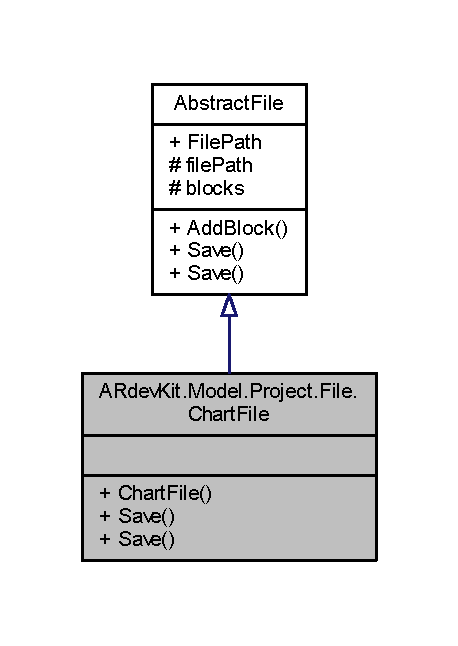
\includegraphics[width=220pt]{class_a_rdev_kit_1_1_model_1_1_project_1_1_file_1_1_chart_file__inherit__graph}
\end{center}
\end{figure}


Collaboration diagram for A\-Rdev\-Kit.\-Model.\-Project.\-File.\-Chart\-File\-:
\nopagebreak
\begin{figure}[H]
\begin{center}
\leavevmode
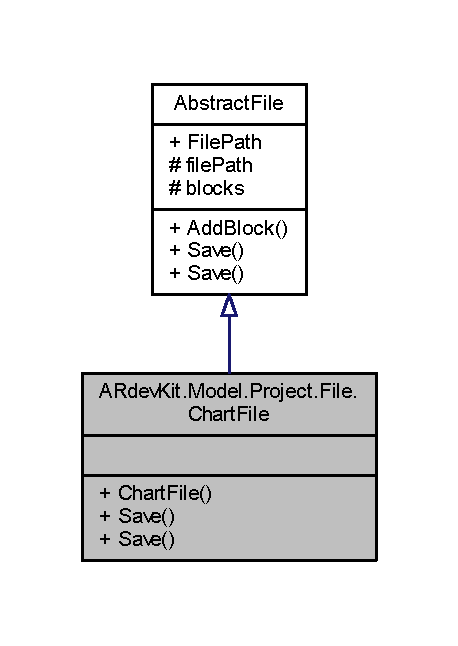
\includegraphics[width=220pt]{class_a_rdev_kit_1_1_model_1_1_project_1_1_file_1_1_chart_file__coll__graph}
\end{center}
\end{figure}
\subsection*{Public Member Functions}
\begin{DoxyCompactItemize}
\item 
\hyperlink{class_a_rdev_kit_1_1_model_1_1_project_1_1_file_1_1_chart_file_a92735bc01ffce6880f8d0f0e2cf499fb}{Chart\-File} (string project\-Path, string chart\-I\-D)
\begin{DoxyCompactList}\small\item\em Constructor. \end{DoxyCompactList}\item 
override void \hyperlink{class_a_rdev_kit_1_1_model_1_1_project_1_1_file_1_1_chart_file_aa19af3145e3bbcb28683e7c77571d06f}{Save} ()
\begin{DoxyCompactList}\small\item\em Saves the file to its \hyperlink{class_a_rdev_kit_1_1_model_1_1_project_1_1_file_1_1_abstract_file_ad879e3a81860da8b72f2d9f61a18ab3b}{file\-Path}. \end{DoxyCompactList}\item 
override void \hyperlink{class_a_rdev_kit_1_1_model_1_1_project_1_1_file_1_1_chart_file_a8a52e5730191b832eb8664016e7bda7f}{Save} (string project\-Path)
\begin{DoxyCompactList}\small\item\em Saves the file to the using the passed project\-Path. \end{DoxyCompactList}\end{DoxyCompactItemize}
\subsection*{Additional Inherited Members}


\subsection{Detailed Description}
A \hyperlink{class_a_rdev_kit_1_1_model_1_1_project_1_1_file_1_1_chart_file}{Chart\-File} is an \hyperlink{class_a_rdev_kit_1_1_model_1_1_project_1_1_file_1_1_abstract_file}{Abstract\-File} which represents the chart.\-js. 



\subsection{Constructor \& Destructor Documentation}
\hypertarget{class_a_rdev_kit_1_1_model_1_1_project_1_1_file_1_1_chart_file_a92735bc01ffce6880f8d0f0e2cf499fb}{\index{A\-Rdev\-Kit\-::\-Model\-::\-Project\-::\-File\-::\-Chart\-File@{A\-Rdev\-Kit\-::\-Model\-::\-Project\-::\-File\-::\-Chart\-File}!Chart\-File@{Chart\-File}}
\index{Chart\-File@{Chart\-File}!ARdevKit::Model::Project::File::ChartFile@{A\-Rdev\-Kit\-::\-Model\-::\-Project\-::\-File\-::\-Chart\-File}}
\subsubsection[{Chart\-File}]{\setlength{\rightskip}{0pt plus 5cm}A\-Rdev\-Kit.\-Model.\-Project.\-File.\-Chart\-File.\-Chart\-File (
\begin{DoxyParamCaption}
\item[{string}]{project\-Path, }
\item[{string}]{chart\-I\-D}
\end{DoxyParamCaption}
)}}\label{class_a_rdev_kit_1_1_model_1_1_project_1_1_file_1_1_chart_file_a92735bc01ffce6880f8d0f0e2cf499fb}


Constructor. 

Imanuel, 23.\-01.\-2014. 


\begin{DoxyParams}{Parameters}
{\em project\-Path} & The project path to write. \\
\hline
{\em chart\-I\-D} & Identifier for the chart. \\
\hline
\end{DoxyParams}


\subsection{Member Function Documentation}
\hypertarget{class_a_rdev_kit_1_1_model_1_1_project_1_1_file_1_1_chart_file_aa19af3145e3bbcb28683e7c77571d06f}{\index{A\-Rdev\-Kit\-::\-Model\-::\-Project\-::\-File\-::\-Chart\-File@{A\-Rdev\-Kit\-::\-Model\-::\-Project\-::\-File\-::\-Chart\-File}!Save@{Save}}
\index{Save@{Save}!ARdevKit::Model::Project::File::ChartFile@{A\-Rdev\-Kit\-::\-Model\-::\-Project\-::\-File\-::\-Chart\-File}}
\subsubsection[{Save}]{\setlength{\rightskip}{0pt plus 5cm}override void A\-Rdev\-Kit.\-Model.\-Project.\-File.\-Chart\-File.\-Save (
\begin{DoxyParamCaption}
{}
\end{DoxyParamCaption}
)\hspace{0.3cm}{\ttfamily [virtual]}}}\label{class_a_rdev_kit_1_1_model_1_1_project_1_1_file_1_1_chart_file_aa19af3145e3bbcb28683e7c77571d06f}


Saves the file to its \hyperlink{class_a_rdev_kit_1_1_model_1_1_project_1_1_file_1_1_abstract_file_ad879e3a81860da8b72f2d9f61a18ab3b}{file\-Path}. 

Imanuel, 23.\-01.\-2014. 

Implements \hyperlink{class_a_rdev_kit_1_1_model_1_1_project_1_1_file_1_1_abstract_file_a095ebaeca96a6d285d9caff1ad726d5b}{A\-Rdev\-Kit.\-Model.\-Project.\-File.\-Abstract\-File}.

\hypertarget{class_a_rdev_kit_1_1_model_1_1_project_1_1_file_1_1_chart_file_a8a52e5730191b832eb8664016e7bda7f}{\index{A\-Rdev\-Kit\-::\-Model\-::\-Project\-::\-File\-::\-Chart\-File@{A\-Rdev\-Kit\-::\-Model\-::\-Project\-::\-File\-::\-Chart\-File}!Save@{Save}}
\index{Save@{Save}!ARdevKit::Model::Project::File::ChartFile@{A\-Rdev\-Kit\-::\-Model\-::\-Project\-::\-File\-::\-Chart\-File}}
\subsubsection[{Save}]{\setlength{\rightskip}{0pt plus 5cm}override void A\-Rdev\-Kit.\-Model.\-Project.\-File.\-Chart\-File.\-Save (
\begin{DoxyParamCaption}
\item[{string}]{project\-Path}
\end{DoxyParamCaption}
)\hspace{0.3cm}{\ttfamily [virtual]}}}\label{class_a_rdev_kit_1_1_model_1_1_project_1_1_file_1_1_chart_file_a8a52e5730191b832eb8664016e7bda7f}


Saves the file to the using the passed project\-Path. 

Imanuel, 23.\-01.\-2014. 


\begin{DoxyParams}{Parameters}
{\em project\-Path} & The project path to write. \\
\hline
\end{DoxyParams}


Implements \hyperlink{class_a_rdev_kit_1_1_model_1_1_project_1_1_file_1_1_abstract_file_ae49c3262c59642e8f519d0655bbbbbab}{A\-Rdev\-Kit.\-Model.\-Project.\-File.\-Abstract\-File}.


\hypertarget{class_a_rdev_kit_1_1_model_1_1_project_1_1_chart_positioning}{\section{A\-Rdev\-Kit.\-Model.\-Project.\-Chart\-Positioning Class Reference}
\label{class_a_rdev_kit_1_1_model_1_1_project_1_1_chart_positioning}\index{A\-Rdev\-Kit.\-Model.\-Project.\-Chart\-Positioning@{A\-Rdev\-Kit.\-Model.\-Project.\-Chart\-Positioning}}
}


Used to set the position of a chart used by High\-Chart.  




Collaboration diagram for A\-Rdev\-Kit.\-Model.\-Project.\-Chart\-Positioning\-:
\nopagebreak
\begin{figure}[H]
\begin{center}
\leavevmode
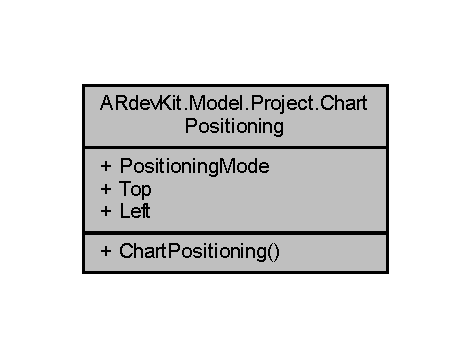
\includegraphics[width=226pt]{class_a_rdev_kit_1_1_model_1_1_project_1_1_chart_positioning__coll__graph}
\end{center}
\end{figure}
\subsection*{Public Types}
\begin{DoxyCompactItemize}
\item 
enum \hyperlink{class_a_rdev_kit_1_1_model_1_1_project_1_1_chart_positioning_ab74042f3d8ce77f994987c15831d76a2}{Positioning\-Modes} \{ {\bfseries S\-T\-A\-T\-I\-C}, 
{\bfseries A\-B\-S\-O\-L\-U\-T\-E}, 
{\bfseries R\-E\-L\-A\-T\-I\-V\-E}
 \}
\begin{DoxyCompactList}\small\item\em Values that represent positioning modes. \end{DoxyCompactList}\end{DoxyCompactItemize}
\subsection*{Public Member Functions}
\begin{DoxyCompactItemize}
\item 
\hyperlink{class_a_rdev_kit_1_1_model_1_1_project_1_1_chart_positioning_a7e26c81e7d9989be224634e219cb4dc2}{Chart\-Positioning} (\hyperlink{class_a_rdev_kit_1_1_model_1_1_project_1_1_chart_positioning_ab74042f3d8ce77f994987c15831d76a2}{Positioning\-Modes} positioning\-Mode)
\begin{DoxyCompactList}\small\item\em Constructor. \end{DoxyCompactList}\end{DoxyCompactItemize}
\subsection*{Properties}
\begin{DoxyCompactItemize}
\item 
\hyperlink{class_a_rdev_kit_1_1_model_1_1_project_1_1_chart_positioning_ab74042f3d8ce77f994987c15831d76a2}{Positioning\-Modes} \hyperlink{class_a_rdev_kit_1_1_model_1_1_project_1_1_chart_positioning_adae5996b4fe2ac69c164ab256037ec5f}{Positioning\-Mode}\hspace{0.3cm}{\ttfamily  \mbox{[}get, set\mbox{]}}
\begin{DoxyCompactList}\small\item\em Gets or sets the positioning mode. \end{DoxyCompactList}\item 
int \hyperlink{class_a_rdev_kit_1_1_model_1_1_project_1_1_chart_positioning_a0853d6ce2e37038ba62f051285ebf2ca}{Top}\hspace{0.3cm}{\ttfamily  \mbox{[}get, set\mbox{]}}
\begin{DoxyCompactList}\small\item\em Gets or sets the top. \end{DoxyCompactList}\item 
int \hyperlink{class_a_rdev_kit_1_1_model_1_1_project_1_1_chart_positioning_adc4b121079440c2d28c2ac86f7ee200a}{Left}\hspace{0.3cm}{\ttfamily  \mbox{[}get, set\mbox{]}}
\begin{DoxyCompactList}\small\item\em Gets or sets the left. \end{DoxyCompactList}\end{DoxyCompactItemize}


\subsection{Detailed Description}
Used to set the position of a chart used by High\-Chart. 

Imanuel, 20.\-01.\-2014. 

\subsection{Member Enumeration Documentation}
\hypertarget{class_a_rdev_kit_1_1_model_1_1_project_1_1_chart_positioning_ab74042f3d8ce77f994987c15831d76a2}{\index{A\-Rdev\-Kit\-::\-Model\-::\-Project\-::\-Chart\-Positioning@{A\-Rdev\-Kit\-::\-Model\-::\-Project\-::\-Chart\-Positioning}!Positioning\-Modes@{Positioning\-Modes}}
\index{Positioning\-Modes@{Positioning\-Modes}!ARdevKit::Model::Project::ChartPositioning@{A\-Rdev\-Kit\-::\-Model\-::\-Project\-::\-Chart\-Positioning}}
\subsubsection[{Positioning\-Modes}]{\setlength{\rightskip}{0pt plus 5cm}enum {\bf A\-Rdev\-Kit.\-Model.\-Project.\-Chart\-Positioning.\-Positioning\-Modes}}}\label{class_a_rdev_kit_1_1_model_1_1_project_1_1_chart_positioning_ab74042f3d8ce77f994987c15831d76a2}


Values that represent positioning modes. 

Imanuel, 27.\-01.\-2014. 

\subsection{Constructor \& Destructor Documentation}
\hypertarget{class_a_rdev_kit_1_1_model_1_1_project_1_1_chart_positioning_a7e26c81e7d9989be224634e219cb4dc2}{\index{A\-Rdev\-Kit\-::\-Model\-::\-Project\-::\-Chart\-Positioning@{A\-Rdev\-Kit\-::\-Model\-::\-Project\-::\-Chart\-Positioning}!Chart\-Positioning@{Chart\-Positioning}}
\index{Chart\-Positioning@{Chart\-Positioning}!ARdevKit::Model::Project::ChartPositioning@{A\-Rdev\-Kit\-::\-Model\-::\-Project\-::\-Chart\-Positioning}}
\subsubsection[{Chart\-Positioning}]{\setlength{\rightskip}{0pt plus 5cm}A\-Rdev\-Kit.\-Model.\-Project.\-Chart\-Positioning.\-Chart\-Positioning (
\begin{DoxyParamCaption}
\item[{{\bf Positioning\-Modes}}]{positioning\-Mode}
\end{DoxyParamCaption}
)}}\label{class_a_rdev_kit_1_1_model_1_1_project_1_1_chart_positioning_a7e26c81e7d9989be224634e219cb4dc2}


Constructor. 

Imanuel, 27.\-01.\-2014. 


\begin{DoxyParams}{Parameters}
{\em positioning\-Mode} & The position. \\
\hline
\end{DoxyParams}


\subsection{Property Documentation}
\hypertarget{class_a_rdev_kit_1_1_model_1_1_project_1_1_chart_positioning_adc4b121079440c2d28c2ac86f7ee200a}{\index{A\-Rdev\-Kit\-::\-Model\-::\-Project\-::\-Chart\-Positioning@{A\-Rdev\-Kit\-::\-Model\-::\-Project\-::\-Chart\-Positioning}!Left@{Left}}
\index{Left@{Left}!ARdevKit::Model::Project::ChartPositioning@{A\-Rdev\-Kit\-::\-Model\-::\-Project\-::\-Chart\-Positioning}}
\subsubsection[{Left}]{\setlength{\rightskip}{0pt plus 5cm}int A\-Rdev\-Kit.\-Model.\-Project.\-Chart\-Positioning.\-Left\hspace{0.3cm}{\ttfamily [get]}, {\ttfamily [set]}}}\label{class_a_rdev_kit_1_1_model_1_1_project_1_1_chart_positioning_adc4b121079440c2d28c2ac86f7ee200a}


Gets or sets the left. 

The left. \hypertarget{class_a_rdev_kit_1_1_model_1_1_project_1_1_chart_positioning_adae5996b4fe2ac69c164ab256037ec5f}{\index{A\-Rdev\-Kit\-::\-Model\-::\-Project\-::\-Chart\-Positioning@{A\-Rdev\-Kit\-::\-Model\-::\-Project\-::\-Chart\-Positioning}!Positioning\-Mode@{Positioning\-Mode}}
\index{Positioning\-Mode@{Positioning\-Mode}!ARdevKit::Model::Project::ChartPositioning@{A\-Rdev\-Kit\-::\-Model\-::\-Project\-::\-Chart\-Positioning}}
\subsubsection[{Positioning\-Mode}]{\setlength{\rightskip}{0pt plus 5cm}{\bf Positioning\-Modes} A\-Rdev\-Kit.\-Model.\-Project.\-Chart\-Positioning.\-Positioning\-Mode\hspace{0.3cm}{\ttfamily [get]}, {\ttfamily [set]}}}\label{class_a_rdev_kit_1_1_model_1_1_project_1_1_chart_positioning_adae5996b4fe2ac69c164ab256037ec5f}


Gets or sets the positioning mode. 

The positioning mode. \hypertarget{class_a_rdev_kit_1_1_model_1_1_project_1_1_chart_positioning_a0853d6ce2e37038ba62f051285ebf2ca}{\index{A\-Rdev\-Kit\-::\-Model\-::\-Project\-::\-Chart\-Positioning@{A\-Rdev\-Kit\-::\-Model\-::\-Project\-::\-Chart\-Positioning}!Top@{Top}}
\index{Top@{Top}!ARdevKit::Model::Project::ChartPositioning@{A\-Rdev\-Kit\-::\-Model\-::\-Project\-::\-Chart\-Positioning}}
\subsubsection[{Top}]{\setlength{\rightskip}{0pt plus 5cm}int A\-Rdev\-Kit.\-Model.\-Project.\-Chart\-Positioning.\-Top\hspace{0.3cm}{\ttfamily [get]}, {\ttfamily [set]}}}\label{class_a_rdev_kit_1_1_model_1_1_project_1_1_chart_positioning_a0853d6ce2e37038ba62f051285ebf2ca}


Gets or sets the top. 

The top. 
\hypertarget{class_a_rdev_kit_1_1_model_1_1_project_1_1_custom_user_event}{\section{A\-Rdev\-Kit.\-Model.\-Project.\-Custom\-User\-Event Class Reference}
\label{class_a_rdev_kit_1_1_model_1_1_project_1_1_custom_user_event}\index{A\-Rdev\-Kit.\-Model.\-Project.\-Custom\-User\-Event@{A\-Rdev\-Kit.\-Model.\-Project.\-Custom\-User\-Event}}
}


The class \hyperlink{class_a_rdev_kit_1_1_model_1_1_project_1_1_custom_user_event}{Custom\-User\-Event} mainly contains a reference to a file, which is in the /current\-Project/ Folder. This file has A\-L\-L Events the user creates (inclusive the template events we provide) for O\-N\-E augmentation.  




Collaboration diagram for A\-Rdev\-Kit.\-Model.\-Project.\-Custom\-User\-Event\-:
\nopagebreak
\begin{figure}[H]
\begin{center}
\leavevmode
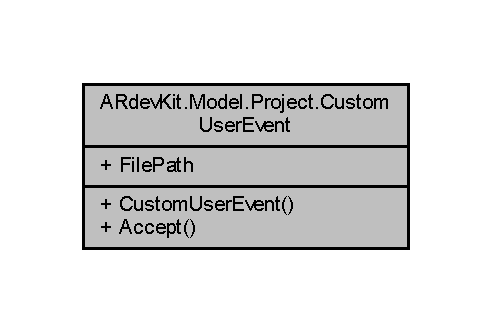
\includegraphics[width=236pt]{class_a_rdev_kit_1_1_model_1_1_project_1_1_custom_user_event__coll__graph}
\end{center}
\end{figure}
\subsection*{Public Member Functions}
\begin{DoxyCompactItemize}
\item 
\hyperlink{class_a_rdev_kit_1_1_model_1_1_project_1_1_custom_user_event_a57e6abd6b60a1b156cc6f025b5ba8e0e}{Custom\-User\-Event} (string augmentation\-I\-D)
\begin{DoxyCompactList}\small\item\em Constructor of the \hyperlink{class_a_rdev_kit_1_1_model_1_1_project_1_1_custom_user_event}{Custom\-User\-Event}. \end{DoxyCompactList}\item 
void \hyperlink{class_a_rdev_kit_1_1_model_1_1_project_1_1_custom_user_event_aa652f9348729297a9749aafa5a3efefb}{Accept} (\hyperlink{class_a_rdev_kit_1_1_controller_1_1_project_controller_1_1_abstract_project_visitor}{Abstract\-Project\-Visitor} visitor)
\begin{DoxyCompactList}\small\item\em A method, to accept a Abstract\-Project\-Visitor which must be implemented according to the visitor design pattern. \end{DoxyCompactList}\end{DoxyCompactItemize}
\subsection*{Properties}
\begin{DoxyCompactItemize}
\item 
string \hyperlink{class_a_rdev_kit_1_1_model_1_1_project_1_1_custom_user_event_a2160a1e51911b3771b96f45d6ba6f214}{File\-Path}\hspace{0.3cm}{\ttfamily  \mbox{[}get, set\mbox{]}}
\begin{DoxyCompactList}\small\item\em Get or set the file path for the custom\-User\-Events-\/\-File. \end{DoxyCompactList}\end{DoxyCompactItemize}


\subsection{Detailed Description}
The class \hyperlink{class_a_rdev_kit_1_1_model_1_1_project_1_1_custom_user_event}{Custom\-User\-Event} mainly contains a reference to a file, which is in the /current\-Project/ Folder. This file has A\-L\-L Events the user creates (inclusive the template events we provide) for O\-N\-E augmentation. 



\subsection{Constructor \& Destructor Documentation}
\hypertarget{class_a_rdev_kit_1_1_model_1_1_project_1_1_custom_user_event_a57e6abd6b60a1b156cc6f025b5ba8e0e}{\index{A\-Rdev\-Kit\-::\-Model\-::\-Project\-::\-Custom\-User\-Event@{A\-Rdev\-Kit\-::\-Model\-::\-Project\-::\-Custom\-User\-Event}!Custom\-User\-Event@{Custom\-User\-Event}}
\index{Custom\-User\-Event@{Custom\-User\-Event}!ARdevKit::Model::Project::CustomUserEvent@{A\-Rdev\-Kit\-::\-Model\-::\-Project\-::\-Custom\-User\-Event}}
\subsubsection[{Custom\-User\-Event}]{\setlength{\rightskip}{0pt plus 5cm}A\-Rdev\-Kit.\-Model.\-Project.\-Custom\-User\-Event.\-Custom\-User\-Event (
\begin{DoxyParamCaption}
\item[{string}]{augmentation\-I\-D}
\end{DoxyParamCaption}
)}}\label{class_a_rdev_kit_1_1_model_1_1_project_1_1_custom_user_event_a57e6abd6b60a1b156cc6f025b5ba8e0e}


Constructor of the \hyperlink{class_a_rdev_kit_1_1_model_1_1_project_1_1_custom_user_event}{Custom\-User\-Event}. 


\begin{DoxyParams}{Parameters}
{\em augmentation\-I\-D} & I\-D of the augmentation\\
\hline
\end{DoxyParams}


\subsection{Member Function Documentation}
\hypertarget{class_a_rdev_kit_1_1_model_1_1_project_1_1_custom_user_event_aa652f9348729297a9749aafa5a3efefb}{\index{A\-Rdev\-Kit\-::\-Model\-::\-Project\-::\-Custom\-User\-Event@{A\-Rdev\-Kit\-::\-Model\-::\-Project\-::\-Custom\-User\-Event}!Accept@{Accept}}
\index{Accept@{Accept}!ARdevKit::Model::Project::CustomUserEvent@{A\-Rdev\-Kit\-::\-Model\-::\-Project\-::\-Custom\-User\-Event}}
\subsubsection[{Accept}]{\setlength{\rightskip}{0pt plus 5cm}void A\-Rdev\-Kit.\-Model.\-Project.\-Custom\-User\-Event.\-Accept (
\begin{DoxyParamCaption}
\item[{{\bf Abstract\-Project\-Visitor}}]{visitor}
\end{DoxyParamCaption}
)}}\label{class_a_rdev_kit_1_1_model_1_1_project_1_1_custom_user_event_aa652f9348729297a9749aafa5a3efefb}


A method, to accept a Abstract\-Project\-Visitor which must be implemented according to the visitor design pattern. 


\begin{DoxyParams}{Parameters}
{\em visitor} & the visitor which encapsulates the action which is performed on this \hyperlink{class_a_rdev_kit_1_1_model_1_1_project_1_1_custom_user_event}{Custom\-User\-Event}\\
\hline
\end{DoxyParams}


\subsection{Property Documentation}
\hypertarget{class_a_rdev_kit_1_1_model_1_1_project_1_1_custom_user_event_a2160a1e51911b3771b96f45d6ba6f214}{\index{A\-Rdev\-Kit\-::\-Model\-::\-Project\-::\-Custom\-User\-Event@{A\-Rdev\-Kit\-::\-Model\-::\-Project\-::\-Custom\-User\-Event}!File\-Path@{File\-Path}}
\index{File\-Path@{File\-Path}!ARdevKit::Model::Project::CustomUserEvent@{A\-Rdev\-Kit\-::\-Model\-::\-Project\-::\-Custom\-User\-Event}}
\subsubsection[{File\-Path}]{\setlength{\rightskip}{0pt plus 5cm}string A\-Rdev\-Kit.\-Model.\-Project.\-Custom\-User\-Event.\-File\-Path\hspace{0.3cm}{\ttfamily [get]}, {\ttfamily [set]}}}\label{class_a_rdev_kit_1_1_model_1_1_project_1_1_custom_user_event_a2160a1e51911b3771b96f45d6ba6f214}


Get or set the file path for the custom\-User\-Events-\/\-File. 


\hypertarget{class_a_rdev_kit_1_1_model_1_1_project_1_1_db_source}{\section{A\-Rdev\-Kit.\-Model.\-Project.\-Db\-Source Class Reference}
\label{class_a_rdev_kit_1_1_model_1_1_project_1_1_db_source}\index{A\-Rdev\-Kit.\-Model.\-Project.\-Db\-Source@{A\-Rdev\-Kit.\-Model.\-Project.\-Db\-Source}}
}


A database source  




Inheritance diagram for A\-Rdev\-Kit.\-Model.\-Project.\-Db\-Source\-:
\nopagebreak
\begin{figure}[H]
\begin{center}
\leavevmode
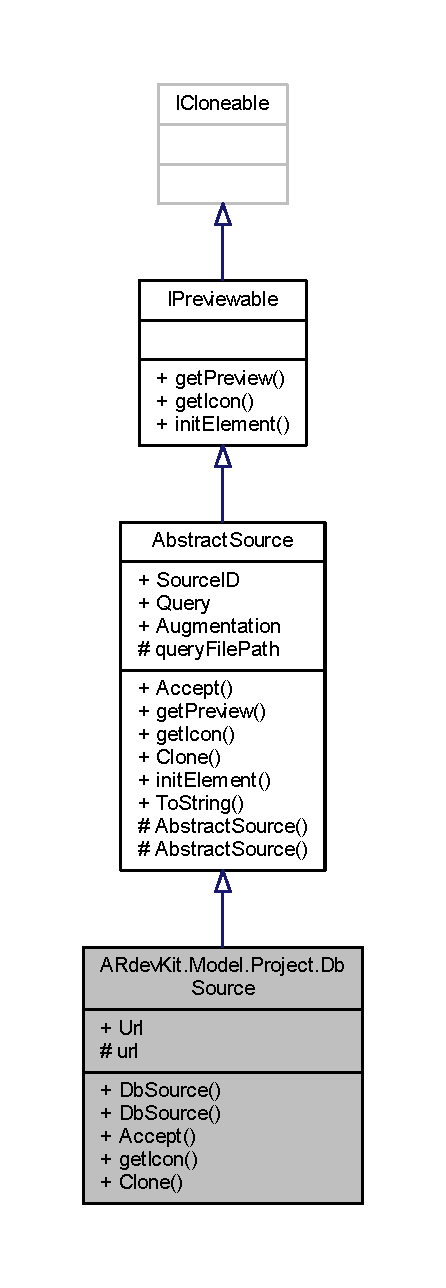
\includegraphics[height=550pt]{class_a_rdev_kit_1_1_model_1_1_project_1_1_db_source__inherit__graph}
\end{center}
\end{figure}


Collaboration diagram for A\-Rdev\-Kit.\-Model.\-Project.\-Db\-Source\-:
\nopagebreak
\begin{figure}[H]
\begin{center}
\leavevmode
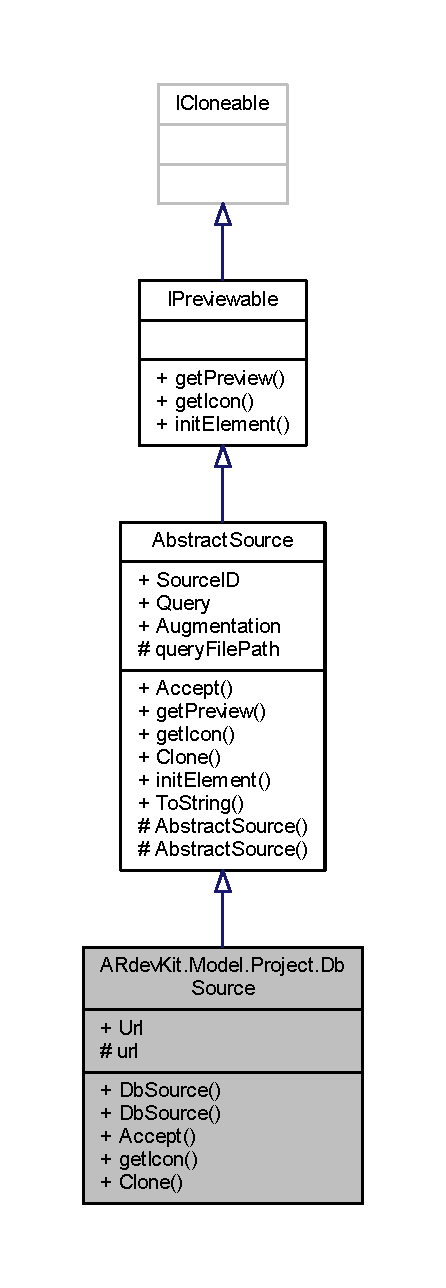
\includegraphics[height=550pt]{class_a_rdev_kit_1_1_model_1_1_project_1_1_db_source__coll__graph}
\end{center}
\end{figure}
\subsection*{Public Member Functions}
\begin{DoxyCompactItemize}
\item 
\hyperlink{class_a_rdev_kit_1_1_model_1_1_project_1_1_db_source_a44cad2325f3fcee5ed95c0a57ada9a1d}{Db\-Source} ()
\begin{DoxyCompactList}\small\item\em Default constructor. \end{DoxyCompactList}\item 
\hyperlink{class_a_rdev_kit_1_1_model_1_1_project_1_1_db_source_a80e5da6929dee8cf0ecb51b4da394df2}{Db\-Source} (string \hyperlink{class_a_rdev_kit_1_1_model_1_1_project_1_1_db_source_ac6b9cc43f2dee23b83d8783c81a07407}{url})
\begin{DoxyCompactList}\small\item\em Constructor. \end{DoxyCompactList}\item 
override void \hyperlink{class_a_rdev_kit_1_1_model_1_1_project_1_1_db_source_aaa7e395578b8e983de0392dd37c55c93}{Accept} (\hyperlink{class_a_rdev_kit_1_1_controller_1_1_project_controller_1_1_abstract_project_visitor}{Abstract\-Project\-Visitor} visitor)
\begin{DoxyCompactList}\small\item\em An abstract method, to accept a Abstract\-Project\-Visitor which must be implemented according to the visitor design pattern. \end{DoxyCompactList}\item 
override Bitmap \hyperlink{class_a_rdev_kit_1_1_model_1_1_project_1_1_db_source_a0890127d66db4ce9c3daa6fe6f44f157}{get\-Icon} ()
\begin{DoxyCompactList}\small\item\em returns a Bitmap in order to be displayed on the Element\-Selection\-Panel, implements \hyperlink{interface_a_rdev_kit_1_1_model_1_1_project_1_1_i_previewable}{I\-Previewable} \end{DoxyCompactList}\item 
override object \hyperlink{class_a_rdev_kit_1_1_model_1_1_project_1_1_db_source_a9c58ffefa3fd6d23d58392273be07d17}{Clone} ()
\begin{DoxyCompactList}\small\item\em Makes a deep copy of this object. \end{DoxyCompactList}\end{DoxyCompactItemize}
\subsection*{Protected Attributes}
\begin{DoxyCompactItemize}
\item 
string \hyperlink{class_a_rdev_kit_1_1_model_1_1_project_1_1_db_source_ac6b9cc43f2dee23b83d8783c81a07407}{url}
\begin{DoxyCompactList}\small\item\em U\-R\-L of the source. \end{DoxyCompactList}\end{DoxyCompactItemize}
\subsection*{Properties}
\begin{DoxyCompactItemize}
\item 
string \hyperlink{class_a_rdev_kit_1_1_model_1_1_project_1_1_db_source_a3a58d6e8914c028e06dbd9ebfef1f4bd}{Url}\hspace{0.3cm}{\ttfamily  \mbox{[}get, set\mbox{]}}
\begin{DoxyCompactList}\small\item\em Gets or sets U\-R\-L of the source. \end{DoxyCompactList}\end{DoxyCompactItemize}
\subsection*{Additional Inherited Members}


\subsection{Detailed Description}
A database source 



\subsection{Constructor \& Destructor Documentation}
\hypertarget{class_a_rdev_kit_1_1_model_1_1_project_1_1_db_source_a44cad2325f3fcee5ed95c0a57ada9a1d}{\index{A\-Rdev\-Kit\-::\-Model\-::\-Project\-::\-Db\-Source@{A\-Rdev\-Kit\-::\-Model\-::\-Project\-::\-Db\-Source}!Db\-Source@{Db\-Source}}
\index{Db\-Source@{Db\-Source}!ARdevKit::Model::Project::DbSource@{A\-Rdev\-Kit\-::\-Model\-::\-Project\-::\-Db\-Source}}
\subsubsection[{Db\-Source}]{\setlength{\rightskip}{0pt plus 5cm}A\-Rdev\-Kit.\-Model.\-Project.\-Db\-Source.\-Db\-Source (
\begin{DoxyParamCaption}
{}
\end{DoxyParamCaption}
)}}\label{class_a_rdev_kit_1_1_model_1_1_project_1_1_db_source_a44cad2325f3fcee5ed95c0a57ada9a1d}


Default constructor. 

Imanuel, 26.\-01.\-2014. \hypertarget{class_a_rdev_kit_1_1_model_1_1_project_1_1_db_source_a80e5da6929dee8cf0ecb51b4da394df2}{\index{A\-Rdev\-Kit\-::\-Model\-::\-Project\-::\-Db\-Source@{A\-Rdev\-Kit\-::\-Model\-::\-Project\-::\-Db\-Source}!Db\-Source@{Db\-Source}}
\index{Db\-Source@{Db\-Source}!ARdevKit::Model::Project::DbSource@{A\-Rdev\-Kit\-::\-Model\-::\-Project\-::\-Db\-Source}}
\subsubsection[{Db\-Source}]{\setlength{\rightskip}{0pt plus 5cm}A\-Rdev\-Kit.\-Model.\-Project.\-Db\-Source.\-Db\-Source (
\begin{DoxyParamCaption}
\item[{string}]{url}
\end{DoxyParamCaption}
)}}\label{class_a_rdev_kit_1_1_model_1_1_project_1_1_db_source_a80e5da6929dee8cf0ecb51b4da394df2}


Constructor. 

Imanuel, 26.\-01.\-2014. 


\begin{DoxyParams}{Parameters}
{\em url} & U\-R\-L of the source. \\
\hline
\end{DoxyParams}


\subsection{Member Function Documentation}
\hypertarget{class_a_rdev_kit_1_1_model_1_1_project_1_1_db_source_aaa7e395578b8e983de0392dd37c55c93}{\index{A\-Rdev\-Kit\-::\-Model\-::\-Project\-::\-Db\-Source@{A\-Rdev\-Kit\-::\-Model\-::\-Project\-::\-Db\-Source}!Accept@{Accept}}
\index{Accept@{Accept}!ARdevKit::Model::Project::DbSource@{A\-Rdev\-Kit\-::\-Model\-::\-Project\-::\-Db\-Source}}
\subsubsection[{Accept}]{\setlength{\rightskip}{0pt plus 5cm}override void A\-Rdev\-Kit.\-Model.\-Project.\-Db\-Source.\-Accept (
\begin{DoxyParamCaption}
\item[{{\bf Abstract\-Project\-Visitor}}]{visitor}
\end{DoxyParamCaption}
)\hspace{0.3cm}{\ttfamily [virtual]}}}\label{class_a_rdev_kit_1_1_model_1_1_project_1_1_db_source_aaa7e395578b8e983de0392dd37c55c93}


An abstract method, to accept a Abstract\-Project\-Visitor which must be implemented according to the visitor design pattern. 

Imanuel, 26.\-01.\-2014. 


\begin{DoxyParams}{Parameters}
{\em visitor} & the visitor which encapsulates the action which is performed on this element. \\
\hline
\end{DoxyParams}


Implements \hyperlink{class_a_rdev_kit_1_1_model_1_1_project_1_1_abstract_source_ad45fa69ac940512f91457ca7c7661882}{A\-Rdev\-Kit.\-Model.\-Project.\-Abstract\-Source}.

\hypertarget{class_a_rdev_kit_1_1_model_1_1_project_1_1_db_source_a9c58ffefa3fd6d23d58392273be07d17}{\index{A\-Rdev\-Kit\-::\-Model\-::\-Project\-::\-Db\-Source@{A\-Rdev\-Kit\-::\-Model\-::\-Project\-::\-Db\-Source}!Clone@{Clone}}
\index{Clone@{Clone}!ARdevKit::Model::Project::DbSource@{A\-Rdev\-Kit\-::\-Model\-::\-Project\-::\-Db\-Source}}
\subsubsection[{Clone}]{\setlength{\rightskip}{0pt plus 5cm}override object A\-Rdev\-Kit.\-Model.\-Project.\-Db\-Source.\-Clone (
\begin{DoxyParamCaption}
{}
\end{DoxyParamCaption}
)\hspace{0.3cm}{\ttfamily [virtual]}}}\label{class_a_rdev_kit_1_1_model_1_1_project_1_1_db_source_a9c58ffefa3fd6d23d58392273be07d17}


Makes a deep copy of this object. 

Robin, 21.\-01.\-2014. 

\begin{DoxyReturn}{Returns}
A copy of this object. 
\end{DoxyReturn}


Implements \hyperlink{class_a_rdev_kit_1_1_model_1_1_project_1_1_abstract_source_a17fb18629481715303c5c55a867bb023}{A\-Rdev\-Kit.\-Model.\-Project.\-Abstract\-Source}.

\hypertarget{class_a_rdev_kit_1_1_model_1_1_project_1_1_db_source_a0890127d66db4ce9c3daa6fe6f44f157}{\index{A\-Rdev\-Kit\-::\-Model\-::\-Project\-::\-Db\-Source@{A\-Rdev\-Kit\-::\-Model\-::\-Project\-::\-Db\-Source}!get\-Icon@{get\-Icon}}
\index{get\-Icon@{get\-Icon}!ARdevKit::Model::Project::DbSource@{A\-Rdev\-Kit\-::\-Model\-::\-Project\-::\-Db\-Source}}
\subsubsection[{get\-Icon}]{\setlength{\rightskip}{0pt plus 5cm}override Bitmap A\-Rdev\-Kit.\-Model.\-Project.\-Db\-Source.\-get\-Icon (
\begin{DoxyParamCaption}
{}
\end{DoxyParamCaption}
)\hspace{0.3cm}{\ttfamily [virtual]}}}\label{class_a_rdev_kit_1_1_model_1_1_project_1_1_db_source_a0890127d66db4ce9c3daa6fe6f44f157}


returns a Bitmap in order to be displayed on the Element\-Selection\-Panel, implements \hyperlink{interface_a_rdev_kit_1_1_model_1_1_project_1_1_i_previewable}{I\-Previewable} 

\begin{DoxyReturn}{Returns}
a representative iconized Bitmap 
\end{DoxyReturn}


Implements \hyperlink{class_a_rdev_kit_1_1_model_1_1_project_1_1_abstract_source_ae698f1c9d55cc0603931bd2804d0c35d}{A\-Rdev\-Kit.\-Model.\-Project.\-Abstract\-Source}.



\subsection{Member Data Documentation}
\hypertarget{class_a_rdev_kit_1_1_model_1_1_project_1_1_db_source_ac6b9cc43f2dee23b83d8783c81a07407}{\index{A\-Rdev\-Kit\-::\-Model\-::\-Project\-::\-Db\-Source@{A\-Rdev\-Kit\-::\-Model\-::\-Project\-::\-Db\-Source}!url@{url}}
\index{url@{url}!ARdevKit::Model::Project::DbSource@{A\-Rdev\-Kit\-::\-Model\-::\-Project\-::\-Db\-Source}}
\subsubsection[{url}]{\setlength{\rightskip}{0pt plus 5cm}string A\-Rdev\-Kit.\-Model.\-Project.\-Db\-Source.\-url\hspace{0.3cm}{\ttfamily [protected]}}}\label{class_a_rdev_kit_1_1_model_1_1_project_1_1_db_source_ac6b9cc43f2dee23b83d8783c81a07407}


U\-R\-L of the source. 



\subsection{Property Documentation}
\hypertarget{class_a_rdev_kit_1_1_model_1_1_project_1_1_db_source_a3a58d6e8914c028e06dbd9ebfef1f4bd}{\index{A\-Rdev\-Kit\-::\-Model\-::\-Project\-::\-Db\-Source@{A\-Rdev\-Kit\-::\-Model\-::\-Project\-::\-Db\-Source}!Url@{Url}}
\index{Url@{Url}!ARdevKit::Model::Project::DbSource@{A\-Rdev\-Kit\-::\-Model\-::\-Project\-::\-Db\-Source}}
\subsubsection[{Url}]{\setlength{\rightskip}{0pt plus 5cm}string A\-Rdev\-Kit.\-Model.\-Project.\-Db\-Source.\-Url\hspace{0.3cm}{\ttfamily [get]}, {\ttfamily [set]}}}\label{class_a_rdev_kit_1_1_model_1_1_project_1_1_db_source_a3a58d6e8914c028e06dbd9ebfef1f4bd}


Gets or sets U\-R\-L of the source. 

The U\-R\-L. 
\hypertarget{class_a_rdev_kit_1_1_view_1_1_debug_window}{\section{A\-Rdev\-Kit.\-View.\-Debug\-Window Class Reference}
\label{class_a_rdev_kit_1_1_view_1_1_debug_window}\index{A\-Rdev\-Kit.\-View.\-Debug\-Window@{A\-Rdev\-Kit.\-View.\-Debug\-Window}}
}


Inheritance diagram for A\-Rdev\-Kit.\-View.\-Debug\-Window\-:
\nopagebreak
\begin{figure}[H]
\begin{center}
\leavevmode
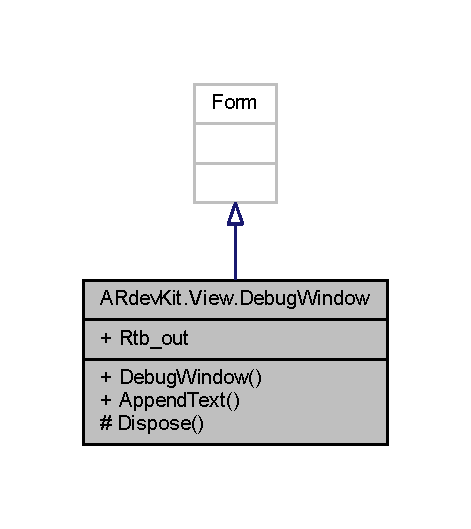
\includegraphics[width=226pt]{class_a_rdev_kit_1_1_view_1_1_debug_window__inherit__graph}
\end{center}
\end{figure}


Collaboration diagram for A\-Rdev\-Kit.\-View.\-Debug\-Window\-:
\nopagebreak
\begin{figure}[H]
\begin{center}
\leavevmode
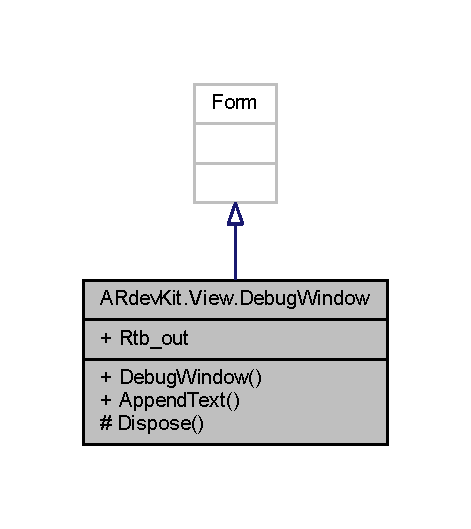
\includegraphics[width=226pt]{class_a_rdev_kit_1_1_view_1_1_debug_window__coll__graph}
\end{center}
\end{figure}
\subsection*{Public Member Functions}
\begin{DoxyCompactItemize}
\item 
\hyperlink{class_a_rdev_kit_1_1_view_1_1_debug_window_adafb78ca129ce982501f18a95a6dfda2}{Debug\-Window} (\hyperlink{class_a_rdev_kit_1_1_controller_1_1_connections_1_1_device_connection_1_1_device_connection_controller}{Controller.\-Connections.\-Device\-Connection.\-Device\-Connection\-Controller} controller)
\begin{DoxyCompactList}\small\item\em Initializes a new instance of the \hyperlink{class_a_rdev_kit_1_1_view_1_1_debug_window}{Debug\-Window} class. \end{DoxyCompactList}\item 
void \hyperlink{class_a_rdev_kit_1_1_view_1_1_debug_window_a699da7b94cba73ded382cbe7d09d259e}{Append\-Text} (string text)
\begin{DoxyCompactList}\small\item\em Appends the text. \end{DoxyCompactList}\end{DoxyCompactItemize}
\subsection*{Protected Member Functions}
\begin{DoxyCompactItemize}
\item 
override void \hyperlink{class_a_rdev_kit_1_1_view_1_1_debug_window_a3fd0798bf834ad179cf33e1e43549e2c}{Dispose} (bool disposing)
\begin{DoxyCompactList}\small\item\em Clean up any resources being used. \end{DoxyCompactList}\end{DoxyCompactItemize}
\subsection*{Properties}
\begin{DoxyCompactItemize}
\item 
System.\-Windows.\-Forms.\-Rich\-Text\-Box \hyperlink{class_a_rdev_kit_1_1_view_1_1_debug_window_a0b6022986bb5968dac5184d2024c6fca}{Rtb\-\_\-out}\hspace{0.3cm}{\ttfamily  \mbox{[}get\mbox{]}}
\begin{DoxyCompactList}\small\item\em Gets the rtb\-\_\-out. \end{DoxyCompactList}\end{DoxyCompactItemize}


\subsection{Constructor \& Destructor Documentation}
\hypertarget{class_a_rdev_kit_1_1_view_1_1_debug_window_adafb78ca129ce982501f18a95a6dfda2}{\index{A\-Rdev\-Kit\-::\-View\-::\-Debug\-Window@{A\-Rdev\-Kit\-::\-View\-::\-Debug\-Window}!Debug\-Window@{Debug\-Window}}
\index{Debug\-Window@{Debug\-Window}!ARdevKit::View::DebugWindow@{A\-Rdev\-Kit\-::\-View\-::\-Debug\-Window}}
\subsubsection[{Debug\-Window}]{\setlength{\rightskip}{0pt plus 5cm}A\-Rdev\-Kit.\-View.\-Debug\-Window.\-Debug\-Window (
\begin{DoxyParamCaption}
\item[{{\bf Controller.\-Connections.\-Device\-Connection.\-Device\-Connection\-Controller}}]{controller}
\end{DoxyParamCaption}
)}}\label{class_a_rdev_kit_1_1_view_1_1_debug_window_adafb78ca129ce982501f18a95a6dfda2}


Initializes a new instance of the \hyperlink{class_a_rdev_kit_1_1_view_1_1_debug_window}{Debug\-Window} class. 


\begin{DoxyParams}{Parameters}
{\em controller} & The controller.\\
\hline
\end{DoxyParams}


\subsection{Member Function Documentation}
\hypertarget{class_a_rdev_kit_1_1_view_1_1_debug_window_a699da7b94cba73ded382cbe7d09d259e}{\index{A\-Rdev\-Kit\-::\-View\-::\-Debug\-Window@{A\-Rdev\-Kit\-::\-View\-::\-Debug\-Window}!Append\-Text@{Append\-Text}}
\index{Append\-Text@{Append\-Text}!ARdevKit::View::DebugWindow@{A\-Rdev\-Kit\-::\-View\-::\-Debug\-Window}}
\subsubsection[{Append\-Text}]{\setlength{\rightskip}{0pt plus 5cm}void A\-Rdev\-Kit.\-View.\-Debug\-Window.\-Append\-Text (
\begin{DoxyParamCaption}
\item[{string}]{text}
\end{DoxyParamCaption}
)}}\label{class_a_rdev_kit_1_1_view_1_1_debug_window_a699da7b94cba73ded382cbe7d09d259e}


Appends the text. 


\begin{DoxyParams}{Parameters}
{\em text} & The text.\\
\hline
\end{DoxyParams}
\hypertarget{class_a_rdev_kit_1_1_view_1_1_debug_window_a3fd0798bf834ad179cf33e1e43549e2c}{\index{A\-Rdev\-Kit\-::\-View\-::\-Debug\-Window@{A\-Rdev\-Kit\-::\-View\-::\-Debug\-Window}!Dispose@{Dispose}}
\index{Dispose@{Dispose}!ARdevKit::View::DebugWindow@{A\-Rdev\-Kit\-::\-View\-::\-Debug\-Window}}
\subsubsection[{Dispose}]{\setlength{\rightskip}{0pt plus 5cm}override void A\-Rdev\-Kit.\-View.\-Debug\-Window.\-Dispose (
\begin{DoxyParamCaption}
\item[{bool}]{disposing}
\end{DoxyParamCaption}
)\hspace{0.3cm}{\ttfamily [protected]}}}\label{class_a_rdev_kit_1_1_view_1_1_debug_window_a3fd0798bf834ad179cf33e1e43549e2c}


Clean up any resources being used. 


\begin{DoxyParams}{Parameters}
{\em disposing} & true if managed resources should be disposed; otherwise, false.\\
\hline
\end{DoxyParams}


\subsection{Property Documentation}
\hypertarget{class_a_rdev_kit_1_1_view_1_1_debug_window_a0b6022986bb5968dac5184d2024c6fca}{\index{A\-Rdev\-Kit\-::\-View\-::\-Debug\-Window@{A\-Rdev\-Kit\-::\-View\-::\-Debug\-Window}!Rtb\-\_\-out@{Rtb\-\_\-out}}
\index{Rtb\-\_\-out@{Rtb\-\_\-out}!ARdevKit::View::DebugWindow@{A\-Rdev\-Kit\-::\-View\-::\-Debug\-Window}}
\subsubsection[{Rtb\-\_\-out}]{\setlength{\rightskip}{0pt plus 5cm}System.\-Windows.\-Forms.\-Rich\-Text\-Box A\-Rdev\-Kit.\-View.\-Debug\-Window.\-Rtb\-\_\-out\hspace{0.3cm}{\ttfamily [get]}}}\label{class_a_rdev_kit_1_1_view_1_1_debug_window_a0b6022986bb5968dac5184d2024c6fca}


Gets the rtb\-\_\-out. 

The rtb\-\_\-out. 
\hypertarget{class_a_rdev_kit_1_1_controller_1_1_connections_1_1_device_connection_1_1_device_connection_controller}{\section{A\-Rdev\-Kit.\-Controller.\-Connections.\-Device\-Connection.\-Device\-Connection\-Controller Class Reference}
\label{class_a_rdev_kit_1_1_controller_1_1_connections_1_1_device_connection_1_1_device_connection_controller}\index{A\-Rdev\-Kit.\-Controller.\-Connections.\-Device\-Connection.\-Device\-Connection\-Controller@{A\-Rdev\-Kit.\-Controller.\-Connections.\-Device\-Connection.\-Device\-Connection\-Controller}}
}


\hyperlink{namespace_a_rdev_kit_1_1_controller}{Controller} which provides functions, to gather Information about Devices, which are running A\-Rdev\-Kit\-Player and are connected to the local Network. On top of that it provides functions to send Projects and receive Debuginformation.  




Collaboration diagram for A\-Rdev\-Kit.\-Controller.\-Connections.\-Device\-Connection.\-Device\-Connection\-Controller\-:
\nopagebreak
\begin{figure}[H]
\begin{center}
\leavevmode
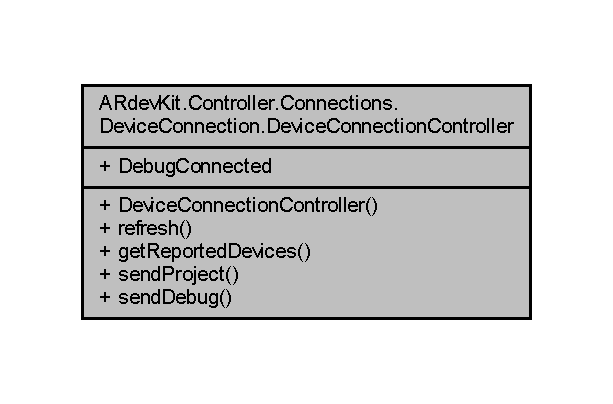
\includegraphics[width=294pt]{class_a_rdev_kit_1_1_controller_1_1_connections_1_1_device_connection_1_1_device_connection_controller__coll__graph}
\end{center}
\end{figure}
\subsection*{Public Member Functions}
\begin{DoxyCompactItemize}
\item 
\hyperlink{class_a_rdev_kit_1_1_controller_1_1_connections_1_1_device_connection_1_1_device_connection_controller_a6d505b2d3b51a10e9d83058157a1c62c}{Device\-Connection\-Controller} (Form window)
\begin{DoxyCompactList}\small\item\em Initializes a new instance of the \hyperlink{class_a_rdev_kit_1_1_controller_1_1_connections_1_1_device_connection_1_1_device_connection_controller}{Device\-Connection\-Controller} class. Uses U\-D\-P\-Listener to get information about devices. Communicating via H\-T\-T\-P order to secure currency of connections and sending the zipped project. \end{DoxyCompactList}\item 
void \hyperlink{class_a_rdev_kit_1_1_controller_1_1_connections_1_1_device_connection_1_1_device_connection_controller_a2fa2baab02402dec9c2dce90fadeb54c}{refresh} ()
\begin{DoxyCompactList}\small\item\em Runs the refresh listener, using a U\-D\-P Broadcast to which the A\-Rdev\-Kit\-Player responds. \end{DoxyCompactList}\item 
List$<$ string $>$ \hyperlink{class_a_rdev_kit_1_1_controller_1_1_connections_1_1_device_connection_1_1_device_connection_controller_a22af53d2338217cf5c77e4f7326cee79}{get\-Reported\-Devices} ()
\begin{DoxyCompactList}\small\item\em Gets the reported devices. \end{DoxyCompactList}\item 
bool \hyperlink{class_a_rdev_kit_1_1_controller_1_1_connections_1_1_device_connection_1_1_device_connection_controller_a4fcdf74b36bf40335dfe5179f78f2524}{send\-Project} (int index)
\begin{DoxyCompactList}\small\item\em Sends the opened Project to the chosen Device, using the selected index of the Editor\-Windows\-Device\-List, which must be equal to the internal index of the reported\-Devices List. Exceptions which are thrown are written to a log file, in the path in which the Program is executed. \end{DoxyCompactList}\item 
bool \hyperlink{class_a_rdev_kit_1_1_controller_1_1_connections_1_1_device_connection_1_1_device_connection_controller_a2810b006ae43957884b041496f4f3498}{send\-Debug} (int index)
\begin{DoxyCompactList}\small\item\em Sends a Debugrequest to the selected Device and shows its Debug\-Output on a Popup\-Window with a Rich\-Textbox \end{DoxyCompactList}\end{DoxyCompactItemize}
\subsection*{Properties}
\begin{DoxyCompactItemize}
\item 
\hyperlink{class_a_rdev_kit_1_1_view_1_1_debug_window}{View.\-Debug\-Window} \hyperlink{class_a_rdev_kit_1_1_controller_1_1_connections_1_1_device_connection_1_1_device_connection_controller_acfe2c36b862f9b0775bf8e0f60d055ad}{Debug\-Window}\hspace{0.3cm}{\ttfamily  \mbox{[}get\mbox{]}}
\begin{DoxyCompactList}\small\item\em Gets the debug window. \end{DoxyCompactList}\item 
bool \hyperlink{class_a_rdev_kit_1_1_controller_1_1_connections_1_1_device_connection_1_1_device_connection_controller_a6e1f49d1912fccc6edc212acbfc74c05}{Debug\-Connected}\hspace{0.3cm}{\ttfamily  \mbox{[}get, set\mbox{]}}
\begin{DoxyCompactList}\small\item\em Gets or sets a value indicating whether \mbox{[}debug connected\mbox{]}. \end{DoxyCompactList}\end{DoxyCompactItemize}


\subsection{Detailed Description}
\hyperlink{namespace_a_rdev_kit_1_1_controller}{Controller} which provides functions, to gather Information about Devices, which are running A\-Rdev\-Kit\-Player and are connected to the local Network. On top of that it provides functions to send Projects and receive Debuginformation. 



\subsection{Constructor \& Destructor Documentation}
\hypertarget{class_a_rdev_kit_1_1_controller_1_1_connections_1_1_device_connection_1_1_device_connection_controller_a6d505b2d3b51a10e9d83058157a1c62c}{\index{A\-Rdev\-Kit\-::\-Controller\-::\-Connections\-::\-Device\-Connection\-::\-Device\-Connection\-Controller@{A\-Rdev\-Kit\-::\-Controller\-::\-Connections\-::\-Device\-Connection\-::\-Device\-Connection\-Controller}!Device\-Connection\-Controller@{Device\-Connection\-Controller}}
\index{Device\-Connection\-Controller@{Device\-Connection\-Controller}!ARdevKit::Controller::Connections::DeviceConnection::DeviceConnectionController@{A\-Rdev\-Kit\-::\-Controller\-::\-Connections\-::\-Device\-Connection\-::\-Device\-Connection\-Controller}}
\subsubsection[{Device\-Connection\-Controller}]{\setlength{\rightskip}{0pt plus 5cm}A\-Rdev\-Kit.\-Controller.\-Connections.\-Device\-Connection.\-Device\-Connection\-Controller.\-Device\-Connection\-Controller (
\begin{DoxyParamCaption}
\item[{Form}]{window}
\end{DoxyParamCaption}
)}}\label{class_a_rdev_kit_1_1_controller_1_1_connections_1_1_device_connection_1_1_device_connection_controller_a6d505b2d3b51a10e9d83058157a1c62c}


Initializes a new instance of the \hyperlink{class_a_rdev_kit_1_1_controller_1_1_connections_1_1_device_connection_1_1_device_connection_controller}{Device\-Connection\-Controller} class. Uses U\-D\-P\-Listener to get information about devices. Communicating via H\-T\-T\-P order to secure currency of connections and sending the zipped project. 


\begin{DoxyParams}{Parameters}
{\em window} & The window.\\
\hline
\end{DoxyParams}


\subsection{Member Function Documentation}
\hypertarget{class_a_rdev_kit_1_1_controller_1_1_connections_1_1_device_connection_1_1_device_connection_controller_a22af53d2338217cf5c77e4f7326cee79}{\index{A\-Rdev\-Kit\-::\-Controller\-::\-Connections\-::\-Device\-Connection\-::\-Device\-Connection\-Controller@{A\-Rdev\-Kit\-::\-Controller\-::\-Connections\-::\-Device\-Connection\-::\-Device\-Connection\-Controller}!get\-Reported\-Devices@{get\-Reported\-Devices}}
\index{get\-Reported\-Devices@{get\-Reported\-Devices}!ARdevKit::Controller::Connections::DeviceConnection::DeviceConnectionController@{A\-Rdev\-Kit\-::\-Controller\-::\-Connections\-::\-Device\-Connection\-::\-Device\-Connection\-Controller}}
\subsubsection[{get\-Reported\-Devices}]{\setlength{\rightskip}{0pt plus 5cm}List$<$string$>$ A\-Rdev\-Kit.\-Controller.\-Connections.\-Device\-Connection.\-Device\-Connection\-Controller.\-get\-Reported\-Devices (
\begin{DoxyParamCaption}
{}
\end{DoxyParamCaption}
)}}\label{class_a_rdev_kit_1_1_controller_1_1_connections_1_1_device_connection_1_1_device_connection_controller_a22af53d2338217cf5c77e4f7326cee79}


Gets the reported devices. 

\begin{DoxyReturn}{Returns}

\end{DoxyReturn}
\hypertarget{class_a_rdev_kit_1_1_controller_1_1_connections_1_1_device_connection_1_1_device_connection_controller_a2fa2baab02402dec9c2dce90fadeb54c}{\index{A\-Rdev\-Kit\-::\-Controller\-::\-Connections\-::\-Device\-Connection\-::\-Device\-Connection\-Controller@{A\-Rdev\-Kit\-::\-Controller\-::\-Connections\-::\-Device\-Connection\-::\-Device\-Connection\-Controller}!refresh@{refresh}}
\index{refresh@{refresh}!ARdevKit::Controller::Connections::DeviceConnection::DeviceConnectionController@{A\-Rdev\-Kit\-::\-Controller\-::\-Connections\-::\-Device\-Connection\-::\-Device\-Connection\-Controller}}
\subsubsection[{refresh}]{\setlength{\rightskip}{0pt plus 5cm}void A\-Rdev\-Kit.\-Controller.\-Connections.\-Device\-Connection.\-Device\-Connection\-Controller.\-refresh (
\begin{DoxyParamCaption}
{}
\end{DoxyParamCaption}
)}}\label{class_a_rdev_kit_1_1_controller_1_1_connections_1_1_device_connection_1_1_device_connection_controller_a2fa2baab02402dec9c2dce90fadeb54c}


Runs the refresh listener, using a U\-D\-P Broadcast to which the A\-Rdev\-Kit\-Player responds. 

\hypertarget{class_a_rdev_kit_1_1_controller_1_1_connections_1_1_device_connection_1_1_device_connection_controller_a2810b006ae43957884b041496f4f3498}{\index{A\-Rdev\-Kit\-::\-Controller\-::\-Connections\-::\-Device\-Connection\-::\-Device\-Connection\-Controller@{A\-Rdev\-Kit\-::\-Controller\-::\-Connections\-::\-Device\-Connection\-::\-Device\-Connection\-Controller}!send\-Debug@{send\-Debug}}
\index{send\-Debug@{send\-Debug}!ARdevKit::Controller::Connections::DeviceConnection::DeviceConnectionController@{A\-Rdev\-Kit\-::\-Controller\-::\-Connections\-::\-Device\-Connection\-::\-Device\-Connection\-Controller}}
\subsubsection[{send\-Debug}]{\setlength{\rightskip}{0pt plus 5cm}bool A\-Rdev\-Kit.\-Controller.\-Connections.\-Device\-Connection.\-Device\-Connection\-Controller.\-send\-Debug (
\begin{DoxyParamCaption}
\item[{int}]{index}
\end{DoxyParamCaption}
)}}\label{class_a_rdev_kit_1_1_controller_1_1_connections_1_1_device_connection_1_1_device_connection_controller_a2810b006ae43957884b041496f4f3498}


Sends a Debugrequest to the selected Device and shows its Debug\-Output on a Popup\-Window with a Rich\-Textbox 


\begin{DoxyParams}{Parameters}
{\em index} & index of the chosen Device\\
\hline
\end{DoxyParams}
\begin{DoxyReturn}{Returns}
true if
\end{DoxyReturn}
\hypertarget{class_a_rdev_kit_1_1_controller_1_1_connections_1_1_device_connection_1_1_device_connection_controller_a4fcdf74b36bf40335dfe5179f78f2524}{\index{A\-Rdev\-Kit\-::\-Controller\-::\-Connections\-::\-Device\-Connection\-::\-Device\-Connection\-Controller@{A\-Rdev\-Kit\-::\-Controller\-::\-Connections\-::\-Device\-Connection\-::\-Device\-Connection\-Controller}!send\-Project@{send\-Project}}
\index{send\-Project@{send\-Project}!ARdevKit::Controller::Connections::DeviceConnection::DeviceConnectionController@{A\-Rdev\-Kit\-::\-Controller\-::\-Connections\-::\-Device\-Connection\-::\-Device\-Connection\-Controller}}
\subsubsection[{send\-Project}]{\setlength{\rightskip}{0pt plus 5cm}bool A\-Rdev\-Kit.\-Controller.\-Connections.\-Device\-Connection.\-Device\-Connection\-Controller.\-send\-Project (
\begin{DoxyParamCaption}
\item[{int}]{index}
\end{DoxyParamCaption}
)}}\label{class_a_rdev_kit_1_1_controller_1_1_connections_1_1_device_connection_1_1_device_connection_controller_a4fcdf74b36bf40335dfe5179f78f2524}


Sends the opened Project to the chosen Device, using the selected index of the Editor\-Windows\-Device\-List, which must be equal to the internal index of the reported\-Devices List. Exceptions which are thrown are written to a log file, in the path in which the Program is executed. 


\begin{DoxyParams}{Parameters}
{\em index} & index of the List of reported\-Devices\\
\hline
\end{DoxyParams}
\begin{DoxyReturn}{Returns}
False, if the project could not be send or an Exception was thown
\end{DoxyReturn}


\subsection{Property Documentation}
\hypertarget{class_a_rdev_kit_1_1_controller_1_1_connections_1_1_device_connection_1_1_device_connection_controller_a6e1f49d1912fccc6edc212acbfc74c05}{\index{A\-Rdev\-Kit\-::\-Controller\-::\-Connections\-::\-Device\-Connection\-::\-Device\-Connection\-Controller@{A\-Rdev\-Kit\-::\-Controller\-::\-Connections\-::\-Device\-Connection\-::\-Device\-Connection\-Controller}!Debug\-Connected@{Debug\-Connected}}
\index{Debug\-Connected@{Debug\-Connected}!ARdevKit::Controller::Connections::DeviceConnection::DeviceConnectionController@{A\-Rdev\-Kit\-::\-Controller\-::\-Connections\-::\-Device\-Connection\-::\-Device\-Connection\-Controller}}
\subsubsection[{Debug\-Connected}]{\setlength{\rightskip}{0pt plus 5cm}bool A\-Rdev\-Kit.\-Controller.\-Connections.\-Device\-Connection.\-Device\-Connection\-Controller.\-Debug\-Connected\hspace{0.3cm}{\ttfamily [get]}, {\ttfamily [set]}}}\label{class_a_rdev_kit_1_1_controller_1_1_connections_1_1_device_connection_1_1_device_connection_controller_a6e1f49d1912fccc6edc212acbfc74c05}


Gets or sets a value indicating whether \mbox{[}debug connected\mbox{]}. 

{\ttfamily true} if \mbox{[}debug connected\mbox{]}; otherwise, {\ttfamily false}. \hypertarget{class_a_rdev_kit_1_1_controller_1_1_connections_1_1_device_connection_1_1_device_connection_controller_acfe2c36b862f9b0775bf8e0f60d055ad}{\index{A\-Rdev\-Kit\-::\-Controller\-::\-Connections\-::\-Device\-Connection\-::\-Device\-Connection\-Controller@{A\-Rdev\-Kit\-::\-Controller\-::\-Connections\-::\-Device\-Connection\-::\-Device\-Connection\-Controller}!Debug\-Window@{Debug\-Window}}
\index{Debug\-Window@{Debug\-Window}!ARdevKit::Controller::Connections::DeviceConnection::DeviceConnectionController@{A\-Rdev\-Kit\-::\-Controller\-::\-Connections\-::\-Device\-Connection\-::\-Device\-Connection\-Controller}}
\subsubsection[{Debug\-Window}]{\setlength{\rightskip}{0pt plus 5cm}{\bf View.\-Debug\-Window} A\-Rdev\-Kit.\-Controller.\-Connections.\-Device\-Connection.\-Device\-Connection\-Controller.\-Debug\-Window\hspace{0.3cm}{\ttfamily [get]}}}\label{class_a_rdev_kit_1_1_controller_1_1_connections_1_1_device_connection_1_1_device_connection_controller_acfe2c36b862f9b0775bf8e0f60d055ad}


Gets the debug window. 

The debug window. 
\hypertarget{class_a_rdev_kit_1_1_editor_window}{\section{A\-Rdev\-Kit.\-Editor\-Window Class Reference}
\label{class_a_rdev_kit_1_1_editor_window}\index{A\-Rdev\-Kit.\-Editor\-Window@{A\-Rdev\-Kit.\-Editor\-Window}}
}


Form for viewing the editor. This is the main form of the program.  




Inheritance diagram for A\-Rdev\-Kit.\-Editor\-Window\-:
\nopagebreak
\begin{figure}[H]
\begin{center}
\leavevmode
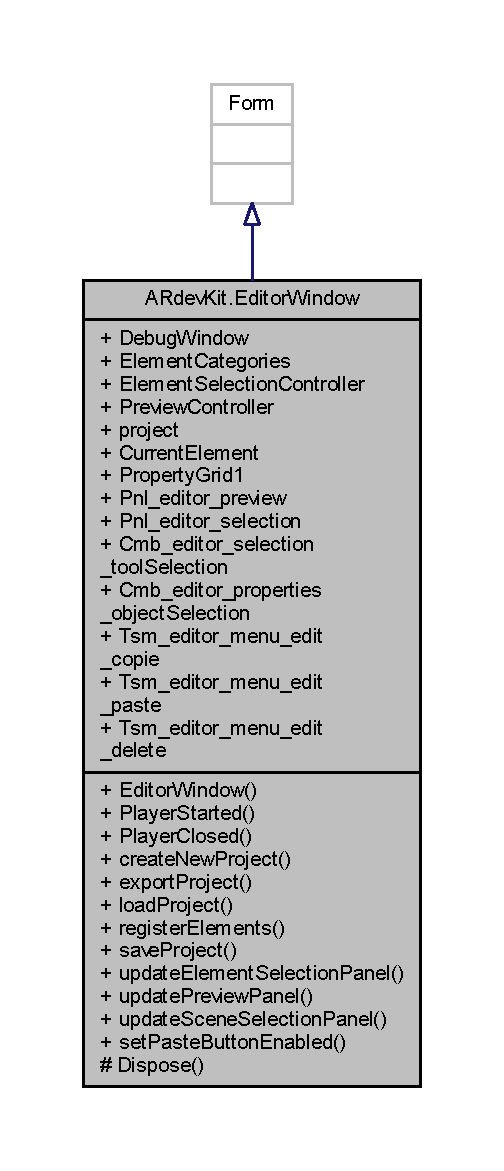
\includegraphics[height=550pt]{class_a_rdev_kit_1_1_editor_window__inherit__graph}
\end{center}
\end{figure}


Collaboration diagram for A\-Rdev\-Kit.\-Editor\-Window\-:
\nopagebreak
\begin{figure}[H]
\begin{center}
\leavevmode
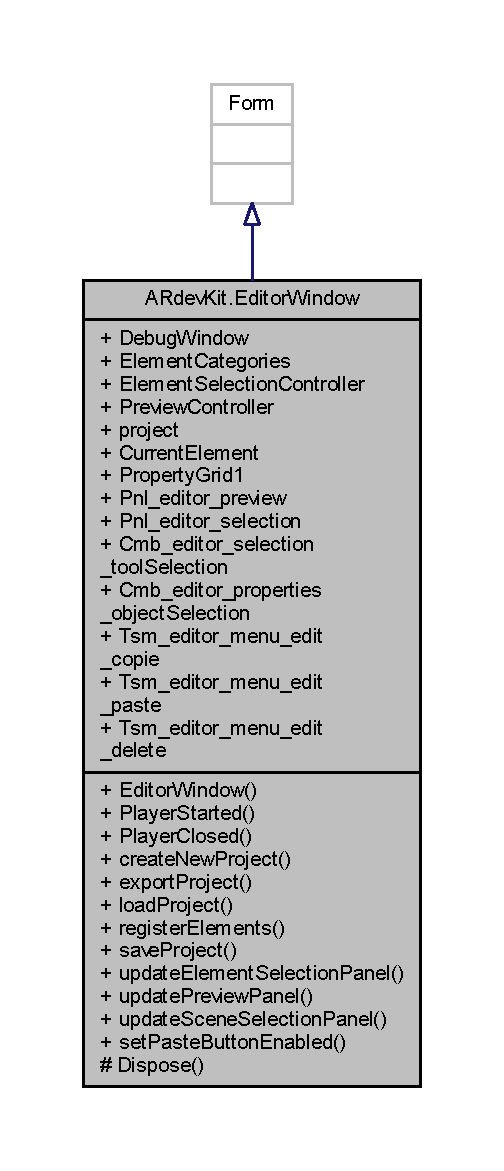
\includegraphics[height=550pt]{class_a_rdev_kit_1_1_editor_window__coll__graph}
\end{center}
\end{figure}
\subsection*{Public Member Functions}
\begin{DoxyCompactItemize}
\item 
\hypertarget{class_a_rdev_kit_1_1_editor_window_aceeacbdb108a82c59f88194a3d4e396c}{\hyperlink{class_a_rdev_kit_1_1_editor_window_aceeacbdb108a82c59f88194a3d4e396c}{Editor\-Window} ()}\label{class_a_rdev_kit_1_1_editor_window_aceeacbdb108a82c59f88194a3d4e396c}

\begin{DoxyCompactList}\small\item\em Default constructor. initializes components on startup. \end{DoxyCompactList}\item 
void \hyperlink{class_a_rdev_kit_1_1_editor_window_a0df48f7d107d823f50799886bd99c1ee}{Player\-Started} ()
\begin{DoxyCompactList}\small\item\em This method is used to tell the editor\-Window that the player was started. \end{DoxyCompactList}\item 
void \hyperlink{class_a_rdev_kit_1_1_editor_window_a03fe5bc5b9e383b895fa1a30faf48301}{Player\-Closed} ()
\begin{DoxyCompactList}\small\item\em This method is used to tell the editor\-Window that the player has been closed. \end{DoxyCompactList}\item 
void \hyperlink{class_a_rdev_kit_1_1_editor_window_afe0bf240a814370f5b119be462a1acec}{create\-New\-Project} (String name)
\begin{DoxyCompactList}\small\item\em Creates the new project. Initialized with the given name. \end{DoxyCompactList}\item 
void \hyperlink{class_a_rdev_kit_1_1_editor_window_a0ae113d771fc8a03dcf53016a54345d4}{export\-Project} ()
\begin{DoxyCompactList}\small\item\em Exports the project. saves the project first and then exports to project path \end{DoxyCompactList}\item 
void \hyperlink{class_a_rdev_kit_1_1_editor_window_a5225f8ebee27d368578165c43f826899}{load\-Project} ()
\begin{DoxyCompactList}\small\item\em Loads the project. Opens a file dialog to select a saved project. \end{DoxyCompactList}\item 
void \hyperlink{class_a_rdev_kit_1_1_editor_window_a62e369fde3e6bf2d3980ff36256a74c1}{register\-Elements} ()
\begin{DoxyCompactList}\small\item\em Registers all Scene\-Elements that are available. \end{DoxyCompactList}\item 
void \hyperlink{class_a_rdev_kit_1_1_editor_window_a7ef9b2d88c9155f213bcc1b0476c4bb2}{save\-Project} ()
\begin{DoxyCompactList}\small\item\em Saves the project. Opens file save dialog if project Path isn't set yet. calls save(\-String path). \end{DoxyCompactList}\item 
void \hyperlink{class_a_rdev_kit_1_1_editor_window_ac2843e3145e7ef49d34dc4b104ff66d4}{update\-Element\-Selection\-Panel} ()
\begin{DoxyCompactList}\small\item\em Updates the element selection panel. (Refreshes the \hyperlink{namespace_a_rdev_kit_1_1_view}{View}) \end{DoxyCompactList}\item 
void \hyperlink{class_a_rdev_kit_1_1_editor_window_a82a2f39ebff57ea65f545b56859be05a}{update\-Preview\-Panel} ()
\begin{DoxyCompactList}\small\item\em This functions Updates the scene Preview\-Panel. Alle elements will be removed and all current elements will add again to the panel. \end{DoxyCompactList}\item 
void \hyperlink{class_a_rdev_kit_1_1_editor_window_abb065a00022ebb57eeb967d319554fc3}{update\-Scene\-Selection\-Panel} ()
\begin{DoxyCompactList}\small\item\em This functions Updates the scene Scene\-Selection\-Panel. Alle elements will be removed and all current elements will add again to the panel. \end{DoxyCompactList}\item 
void \hyperlink{class_a_rdev_kit_1_1_editor_window_a302d58e454127a9fb28eb3fa8b20cc5b}{set\-Paste\-Button\-Enabled} ()
\begin{DoxyCompactList}\small\item\em Sets the Paste\-Button enabled. \end{DoxyCompactList}\end{DoxyCompactItemize}
\subsection*{Protected Member Functions}
\begin{DoxyCompactItemize}
\item 
override void \hyperlink{class_a_rdev_kit_1_1_editor_window_a42208cca445e8fc2eb18e829b5c67d37}{Dispose} (bool disposing)
\begin{DoxyCompactList}\small\item\em Verwendete Ressourcen bereinigen. \end{DoxyCompactList}\end{DoxyCompactItemize}
\subsection*{Properties}
\begin{DoxyCompactItemize}
\item 
\hyperlink{class_a_rdev_kit_1_1_view_1_1_debug_window}{Debug\-Window} \hyperlink{class_a_rdev_kit_1_1_editor_window_a680468ae45b84228fb668d8dbb0aba48}{Debug\-Window}\hspace{0.3cm}{\ttfamily  \mbox{[}get\mbox{]}}
\begin{DoxyCompactList}\small\item\em Gets the debug window. \end{DoxyCompactList}\item 
\hyperlink{class_preview_controller}{Preview\-Controller} \hyperlink{class_a_rdev_kit_1_1_editor_window_ae57e383a1684241c86a5253d1fd8197a}{Preview\-Controller}\hspace{0.3cm}{\ttfamily  \mbox{[}get, set\mbox{]}}
\begin{DoxyCompactList}\small\item\em Gets or sets the preview\-Controller. \end{DoxyCompactList}\item 
\hyperlink{class_a_rdev_kit_1_1_model_1_1_project_1_1_project}{Project} \hyperlink{class_a_rdev_kit_1_1_editor_window_aa7e64c912e3d904fae0ec52588be0baa}{project}\hspace{0.3cm}{\ttfamily  \mbox{[}get, set\mbox{]}}
\begin{DoxyCompactList}\small\item\em Gets or sets the project. \end{DoxyCompactList}\item 
System.\-Windows.\-Forms.\-Property\-Grid \hyperlink{class_a_rdev_kit_1_1_editor_window_a8f5f7c03bcb123e147d07b5023a60292}{Property\-Grid1}\hspace{0.3cm}{\ttfamily  \mbox{[}get, set\mbox{]}}
\begin{DoxyCompactList}\small\item\em Gets or sets the Property\-Grid1. \end{DoxyCompactList}\item 
System.\-Windows.\-Forms.\-Panel \hyperlink{class_a_rdev_kit_1_1_editor_window_a63d02d43b7dfe8841d6e1204948ecb17}{Pnl\-\_\-editor\-\_\-preview}\hspace{0.3cm}{\ttfamily  \mbox{[}get, set\mbox{]}}
\begin{DoxyCompactList}\small\item\em Gets or sets the pnl editor preview. \end{DoxyCompactList}\item 
System.\-Windows.\-Forms.\-Panel \hyperlink{class_a_rdev_kit_1_1_editor_window_a601e295ca226828c6ca4eadc21101a78}{Pnl\-\_\-editor\-\_\-selection}\hspace{0.3cm}{\ttfamily  \mbox{[}get, set\mbox{]}}
\begin{DoxyCompactList}\small\item\em Gets or sets the pnl editor selection. \end{DoxyCompactList}\item 
System.\-Windows.\-Forms.\-Combo\-Box \hyperlink{class_a_rdev_kit_1_1_editor_window_a0937e4db376a67530e488c174d512925}{Cmb\-\_\-editor\-\_\-selection\-\_\-tool\-Selection}\hspace{0.3cm}{\ttfamily  \mbox{[}get, set\mbox{]}}
\begin{DoxyCompactList}\small\item\em Gets or sets the cmb editor selection tool selection. \end{DoxyCompactList}\item 
System.\-Windows.\-Forms.\-Combo\-Box \hyperlink{class_a_rdev_kit_1_1_editor_window_a7a5f59a2277ea660f5ac354ed6563931}{Cmb\-\_\-editor\-\_\-properties\-\_\-object\-Selection}\hspace{0.3cm}{\ttfamily  \mbox{[}get, set\mbox{]}}
\begin{DoxyCompactList}\small\item\em Gets or sets the cmb editor properties object selection. \end{DoxyCompactList}\item 
System.\-Windows.\-Forms.\-Tool\-Strip\-Menu\-Item \hyperlink{class_a_rdev_kit_1_1_editor_window_a7ce809e15aaf06e0d514989fb6292687}{Tsm\-\_\-editor\-\_\-menu\-\_\-edit\-\_\-copie}\hspace{0.3cm}{\ttfamily  \mbox{[}get, set\mbox{]}}
\begin{DoxyCompactList}\small\item\em Gets or sets the tsm\-\_\-editor\-\_\-menu\-\_\-edit\-\_\-copie. \end{DoxyCompactList}\item 
System.\-Windows.\-Forms.\-Tool\-Strip\-Menu\-Item \hyperlink{class_a_rdev_kit_1_1_editor_window_ac2310f24fffc1c84b2c23c5e6cbd8156}{Tsm\-\_\-editor\-\_\-menu\-\_\-edit\-\_\-paste}\hspace{0.3cm}{\ttfamily  \mbox{[}get, set\mbox{]}}
\begin{DoxyCompactList}\small\item\em Gets or sets the tsm\-\_\-editor\-\_\-menu\-\_\-edit\-\_\-paste. \end{DoxyCompactList}\item 
System.\-Windows.\-Forms.\-Tool\-Strip\-Menu\-Item \hyperlink{class_a_rdev_kit_1_1_editor_window_a94b80b86878dae463d966bd117732260}{Tsm\-\_\-editor\-\_\-menu\-\_\-edit\-\_\-delete}\hspace{0.3cm}{\ttfamily  \mbox{[}get, set\mbox{]}}
\begin{DoxyCompactList}\small\item\em Gets or sets the tsm\-\_\-editor\-\_\-menu\-\_\-edit\-\_\-delete. \end{DoxyCompactList}\end{DoxyCompactItemize}


\subsection{Detailed Description}
Form for viewing the editor. This is the main form of the program. 

\subsection{Member Function Documentation}
\hypertarget{class_a_rdev_kit_1_1_editor_window_afe0bf240a814370f5b119be462a1acec}{\index{A\-Rdev\-Kit\-::\-Editor\-Window@{A\-Rdev\-Kit\-::\-Editor\-Window}!create\-New\-Project@{create\-New\-Project}}
\index{create\-New\-Project@{create\-New\-Project}!ARdevKit::EditorWindow@{A\-Rdev\-Kit\-::\-Editor\-Window}}
\subsubsection[{create\-New\-Project}]{\setlength{\rightskip}{0pt plus 5cm}void A\-Rdev\-Kit.\-Editor\-Window.\-create\-New\-Project (
\begin{DoxyParamCaption}
\item[{String}]{name}
\end{DoxyParamCaption}
)}}\label{class_a_rdev_kit_1_1_editor_window_afe0bf240a814370f5b119be462a1acec}


Creates the new project. Initialized with the given name. 


\begin{DoxyParams}{Parameters}
{\em name} & Name of the new project.\\
\hline
\end{DoxyParams}


Here is the caller graph for this function\-:
\nopagebreak
\begin{figure}[H]
\begin{center}
\leavevmode
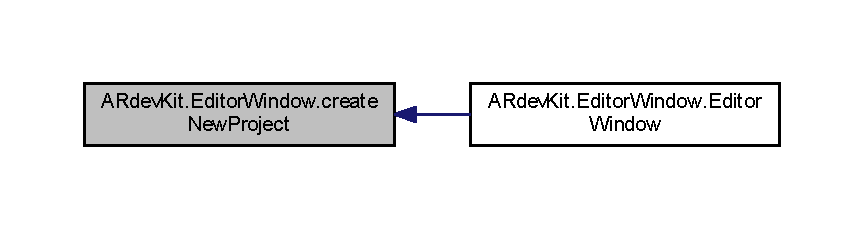
\includegraphics[width=350pt]{class_a_rdev_kit_1_1_editor_window_afe0bf240a814370f5b119be462a1acec_icgraph}
\end{center}
\end{figure}


\hypertarget{class_a_rdev_kit_1_1_editor_window_a42208cca445e8fc2eb18e829b5c67d37}{\index{A\-Rdev\-Kit\-::\-Editor\-Window@{A\-Rdev\-Kit\-::\-Editor\-Window}!Dispose@{Dispose}}
\index{Dispose@{Dispose}!ARdevKit::EditorWindow@{A\-Rdev\-Kit\-::\-Editor\-Window}}
\subsubsection[{Dispose}]{\setlength{\rightskip}{0pt plus 5cm}override void A\-Rdev\-Kit.\-Editor\-Window.\-Dispose (
\begin{DoxyParamCaption}
\item[{bool}]{disposing}
\end{DoxyParamCaption}
)\hspace{0.3cm}{\ttfamily [protected]}}}\label{class_a_rdev_kit_1_1_editor_window_a42208cca445e8fc2eb18e829b5c67d37}


Verwendete Ressourcen bereinigen. 


\begin{DoxyParams}{Parameters}
{\em disposing} & True, wenn verwaltete Ressourcen gelöscht werden sollen; andernfalls False.\\
\hline
\end{DoxyParams}
\hypertarget{class_a_rdev_kit_1_1_editor_window_a0ae113d771fc8a03dcf53016a54345d4}{\index{A\-Rdev\-Kit\-::\-Editor\-Window@{A\-Rdev\-Kit\-::\-Editor\-Window}!export\-Project@{export\-Project}}
\index{export\-Project@{export\-Project}!ARdevKit::EditorWindow@{A\-Rdev\-Kit\-::\-Editor\-Window}}
\subsubsection[{export\-Project}]{\setlength{\rightskip}{0pt plus 5cm}void A\-Rdev\-Kit.\-Editor\-Window.\-export\-Project (
\begin{DoxyParamCaption}
{}
\end{DoxyParamCaption}
)}}\label{class_a_rdev_kit_1_1_editor_window_a0ae113d771fc8a03dcf53016a54345d4}


Exports the project. saves the project first and then exports to project path 

geht 19.\-01.\-2014 22\-:10

Here is the call graph for this function\-:
\nopagebreak
\begin{figure}[H]
\begin{center}
\leavevmode
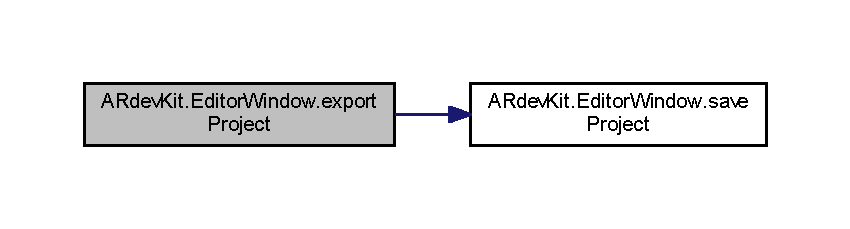
\includegraphics[width=350pt]{class_a_rdev_kit_1_1_editor_window_a0ae113d771fc8a03dcf53016a54345d4_cgraph}
\end{center}
\end{figure}


\hypertarget{class_a_rdev_kit_1_1_editor_window_a5225f8ebee27d368578165c43f826899}{\index{A\-Rdev\-Kit\-::\-Editor\-Window@{A\-Rdev\-Kit\-::\-Editor\-Window}!load\-Project@{load\-Project}}
\index{load\-Project@{load\-Project}!ARdevKit::EditorWindow@{A\-Rdev\-Kit\-::\-Editor\-Window}}
\subsubsection[{load\-Project}]{\setlength{\rightskip}{0pt plus 5cm}void A\-Rdev\-Kit.\-Editor\-Window.\-load\-Project (
\begin{DoxyParamCaption}
{}
\end{DoxyParamCaption}
)}}\label{class_a_rdev_kit_1_1_editor_window_a5225f8ebee27d368578165c43f826899}


Loads the project. Opens a file dialog to select a saved project. 

geht 19.\-01.\-2014 17\-:55\hypertarget{class_a_rdev_kit_1_1_editor_window_a03fe5bc5b9e383b895fa1a30faf48301}{\index{A\-Rdev\-Kit\-::\-Editor\-Window@{A\-Rdev\-Kit\-::\-Editor\-Window}!Player\-Closed@{Player\-Closed}}
\index{Player\-Closed@{Player\-Closed}!ARdevKit::EditorWindow@{A\-Rdev\-Kit\-::\-Editor\-Window}}
\subsubsection[{Player\-Closed}]{\setlength{\rightskip}{0pt plus 5cm}void A\-Rdev\-Kit.\-Editor\-Window.\-Player\-Closed (
\begin{DoxyParamCaption}
{}
\end{DoxyParamCaption}
)}}\label{class_a_rdev_kit_1_1_editor_window_a03fe5bc5b9e383b895fa1a30faf48301}


This method is used to tell the editor\-Window that the player has been closed. 

\hypertarget{class_a_rdev_kit_1_1_editor_window_a0df48f7d107d823f50799886bd99c1ee}{\index{A\-Rdev\-Kit\-::\-Editor\-Window@{A\-Rdev\-Kit\-::\-Editor\-Window}!Player\-Started@{Player\-Started}}
\index{Player\-Started@{Player\-Started}!ARdevKit::EditorWindow@{A\-Rdev\-Kit\-::\-Editor\-Window}}
\subsubsection[{Player\-Started}]{\setlength{\rightskip}{0pt plus 5cm}void A\-Rdev\-Kit.\-Editor\-Window.\-Player\-Started (
\begin{DoxyParamCaption}
{}
\end{DoxyParamCaption}
)}}\label{class_a_rdev_kit_1_1_editor_window_a0df48f7d107d823f50799886bd99c1ee}


This method is used to tell the editor\-Window that the player was started. 

\hypertarget{class_a_rdev_kit_1_1_editor_window_a62e369fde3e6bf2d3980ff36256a74c1}{\index{A\-Rdev\-Kit\-::\-Editor\-Window@{A\-Rdev\-Kit\-::\-Editor\-Window}!register\-Elements@{register\-Elements}}
\index{register\-Elements@{register\-Elements}!ARdevKit::EditorWindow@{A\-Rdev\-Kit\-::\-Editor\-Window}}
\subsubsection[{register\-Elements}]{\setlength{\rightskip}{0pt plus 5cm}void A\-Rdev\-Kit.\-Editor\-Window.\-register\-Elements (
\begin{DoxyParamCaption}
{}
\end{DoxyParamCaption}
)}}\label{class_a_rdev_kit_1_1_editor_window_a62e369fde3e6bf2d3980ff36256a74c1}


Registers all Scene\-Elements that are available. 

Robin, 14.\-01.\-2014. \hypertarget{class_a_rdev_kit_1_1_editor_window_a7ef9b2d88c9155f213bcc1b0476c4bb2}{\index{A\-Rdev\-Kit\-::\-Editor\-Window@{A\-Rdev\-Kit\-::\-Editor\-Window}!save\-Project@{save\-Project}}
\index{save\-Project@{save\-Project}!ARdevKit::EditorWindow@{A\-Rdev\-Kit\-::\-Editor\-Window}}
\subsubsection[{save\-Project}]{\setlength{\rightskip}{0pt plus 5cm}void A\-Rdev\-Kit.\-Editor\-Window.\-save\-Project (
\begin{DoxyParamCaption}
{}
\end{DoxyParamCaption}
)}}\label{class_a_rdev_kit_1_1_editor_window_a7ef9b2d88c9155f213bcc1b0476c4bb2}


Saves the project. Opens file save dialog if project Path isn't set yet. calls save(\-String path). 

geht, 17.\-01.\-2014. 

Here is the caller graph for this function\-:
\nopagebreak
\begin{figure}[H]
\begin{center}
\leavevmode
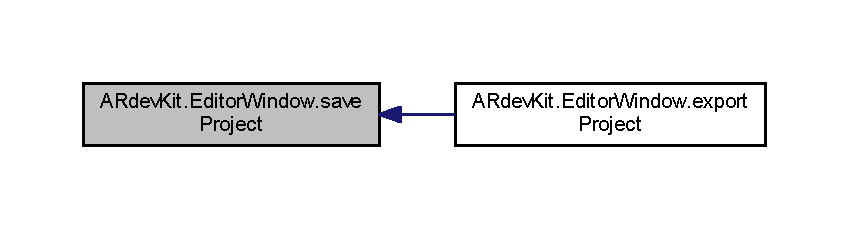
\includegraphics[width=350pt]{class_a_rdev_kit_1_1_editor_window_a7ef9b2d88c9155f213bcc1b0476c4bb2_icgraph}
\end{center}
\end{figure}


\hypertarget{class_a_rdev_kit_1_1_editor_window_a302d58e454127a9fb28eb3fa8b20cc5b}{\index{A\-Rdev\-Kit\-::\-Editor\-Window@{A\-Rdev\-Kit\-::\-Editor\-Window}!set\-Paste\-Button\-Enabled@{set\-Paste\-Button\-Enabled}}
\index{set\-Paste\-Button\-Enabled@{set\-Paste\-Button\-Enabled}!ARdevKit::EditorWindow@{A\-Rdev\-Kit\-::\-Editor\-Window}}
\subsubsection[{set\-Paste\-Button\-Enabled}]{\setlength{\rightskip}{0pt plus 5cm}void A\-Rdev\-Kit.\-Editor\-Window.\-set\-Paste\-Button\-Enabled (
\begin{DoxyParamCaption}
{}
\end{DoxyParamCaption}
)}}\label{class_a_rdev_kit_1_1_editor_window_a302d58e454127a9fb28eb3fa8b20cc5b}


Sets the Paste\-Button enabled. 

\hypertarget{class_a_rdev_kit_1_1_editor_window_ac2843e3145e7ef49d34dc4b104ff66d4}{\index{A\-Rdev\-Kit\-::\-Editor\-Window@{A\-Rdev\-Kit\-::\-Editor\-Window}!update\-Element\-Selection\-Panel@{update\-Element\-Selection\-Panel}}
\index{update\-Element\-Selection\-Panel@{update\-Element\-Selection\-Panel}!ARdevKit::EditorWindow@{A\-Rdev\-Kit\-::\-Editor\-Window}}
\subsubsection[{update\-Element\-Selection\-Panel}]{\setlength{\rightskip}{0pt plus 5cm}void A\-Rdev\-Kit.\-Editor\-Window.\-update\-Element\-Selection\-Panel (
\begin{DoxyParamCaption}
{}
\end{DoxyParamCaption}
)}}\label{class_a_rdev_kit_1_1_editor_window_ac2843e3145e7ef49d34dc4b104ff66d4}


Updates the element selection panel. (Refreshes the \hyperlink{namespace_a_rdev_kit_1_1_view}{View}) 

\hypertarget{class_a_rdev_kit_1_1_editor_window_a82a2f39ebff57ea65f545b56859be05a}{\index{A\-Rdev\-Kit\-::\-Editor\-Window@{A\-Rdev\-Kit\-::\-Editor\-Window}!update\-Preview\-Panel@{update\-Preview\-Panel}}
\index{update\-Preview\-Panel@{update\-Preview\-Panel}!ARdevKit::EditorWindow@{A\-Rdev\-Kit\-::\-Editor\-Window}}
\subsubsection[{update\-Preview\-Panel}]{\setlength{\rightskip}{0pt plus 5cm}void A\-Rdev\-Kit.\-Editor\-Window.\-update\-Preview\-Panel (
\begin{DoxyParamCaption}
{}
\end{DoxyParamCaption}
)}}\label{class_a_rdev_kit_1_1_editor_window_a82a2f39ebff57ea65f545b56859be05a}


This functions Updates the scene Preview\-Panel. Alle elements will be removed and all current elements will add again to the panel. 

Lizzard, 1/16/2014. \hypertarget{class_a_rdev_kit_1_1_editor_window_abb065a00022ebb57eeb967d319554fc3}{\index{A\-Rdev\-Kit\-::\-Editor\-Window@{A\-Rdev\-Kit\-::\-Editor\-Window}!update\-Scene\-Selection\-Panel@{update\-Scene\-Selection\-Panel}}
\index{update\-Scene\-Selection\-Panel@{update\-Scene\-Selection\-Panel}!ARdevKit::EditorWindow@{A\-Rdev\-Kit\-::\-Editor\-Window}}
\subsubsection[{update\-Scene\-Selection\-Panel}]{\setlength{\rightskip}{0pt plus 5cm}void A\-Rdev\-Kit.\-Editor\-Window.\-update\-Scene\-Selection\-Panel (
\begin{DoxyParamCaption}
{}
\end{DoxyParamCaption}
)}}\label{class_a_rdev_kit_1_1_editor_window_abb065a00022ebb57eeb967d319554fc3}


This functions Updates the scene Scene\-Selection\-Panel. Alle elements will be removed and all current elements will add again to the panel. 

Lizzard, 1/16/2014. 

\subsection{Property Documentation}
\hypertarget{class_a_rdev_kit_1_1_editor_window_a7a5f59a2277ea660f5ac354ed6563931}{\index{A\-Rdev\-Kit\-::\-Editor\-Window@{A\-Rdev\-Kit\-::\-Editor\-Window}!Cmb\-\_\-editor\-\_\-properties\-\_\-object\-Selection@{Cmb\-\_\-editor\-\_\-properties\-\_\-object\-Selection}}
\index{Cmb\-\_\-editor\-\_\-properties\-\_\-object\-Selection@{Cmb\-\_\-editor\-\_\-properties\-\_\-object\-Selection}!ARdevKit::EditorWindow@{A\-Rdev\-Kit\-::\-Editor\-Window}}
\subsubsection[{Cmb\-\_\-editor\-\_\-properties\-\_\-object\-Selection}]{\setlength{\rightskip}{0pt plus 5cm}System.\-Windows.\-Forms.\-Combo\-Box A\-Rdev\-Kit.\-Editor\-Window.\-Cmb\-\_\-editor\-\_\-properties\-\_\-object\-Selection\hspace{0.3cm}{\ttfamily [get]}, {\ttfamily [set]}}}\label{class_a_rdev_kit_1_1_editor_window_a7a5f59a2277ea660f5ac354ed6563931}


Gets or sets the cmb editor properties object selection. 

The cmb editor properties object selection. \hypertarget{class_a_rdev_kit_1_1_editor_window_a0937e4db376a67530e488c174d512925}{\index{A\-Rdev\-Kit\-::\-Editor\-Window@{A\-Rdev\-Kit\-::\-Editor\-Window}!Cmb\-\_\-editor\-\_\-selection\-\_\-tool\-Selection@{Cmb\-\_\-editor\-\_\-selection\-\_\-tool\-Selection}}
\index{Cmb\-\_\-editor\-\_\-selection\-\_\-tool\-Selection@{Cmb\-\_\-editor\-\_\-selection\-\_\-tool\-Selection}!ARdevKit::EditorWindow@{A\-Rdev\-Kit\-::\-Editor\-Window}}
\subsubsection[{Cmb\-\_\-editor\-\_\-selection\-\_\-tool\-Selection}]{\setlength{\rightskip}{0pt plus 5cm}System.\-Windows.\-Forms.\-Combo\-Box A\-Rdev\-Kit.\-Editor\-Window.\-Cmb\-\_\-editor\-\_\-selection\-\_\-tool\-Selection\hspace{0.3cm}{\ttfamily [get]}, {\ttfamily [set]}}}\label{class_a_rdev_kit_1_1_editor_window_a0937e4db376a67530e488c174d512925}


Gets or sets the cmb editor selection tool selection. 

The cmb editor selection tool selection. \hypertarget{class_a_rdev_kit_1_1_editor_window_a680468ae45b84228fb668d8dbb0aba48}{\index{A\-Rdev\-Kit\-::\-Editor\-Window@{A\-Rdev\-Kit\-::\-Editor\-Window}!Debug\-Window@{Debug\-Window}}
\index{Debug\-Window@{Debug\-Window}!ARdevKit::EditorWindow@{A\-Rdev\-Kit\-::\-Editor\-Window}}
\subsubsection[{Debug\-Window}]{\setlength{\rightskip}{0pt plus 5cm}{\bf Debug\-Window} A\-Rdev\-Kit.\-Editor\-Window.\-Debug\-Window\hspace{0.3cm}{\ttfamily [get]}}}\label{class_a_rdev_kit_1_1_editor_window_a680468ae45b84228fb668d8dbb0aba48}


Gets the debug window. 

The debug window. \hypertarget{class_a_rdev_kit_1_1_editor_window_a63d02d43b7dfe8841d6e1204948ecb17}{\index{A\-Rdev\-Kit\-::\-Editor\-Window@{A\-Rdev\-Kit\-::\-Editor\-Window}!Pnl\-\_\-editor\-\_\-preview@{Pnl\-\_\-editor\-\_\-preview}}
\index{Pnl\-\_\-editor\-\_\-preview@{Pnl\-\_\-editor\-\_\-preview}!ARdevKit::EditorWindow@{A\-Rdev\-Kit\-::\-Editor\-Window}}
\subsubsection[{Pnl\-\_\-editor\-\_\-preview}]{\setlength{\rightskip}{0pt plus 5cm}System.\-Windows.\-Forms.\-Panel A\-Rdev\-Kit.\-Editor\-Window.\-Pnl\-\_\-editor\-\_\-preview\hspace{0.3cm}{\ttfamily [get]}, {\ttfamily [set]}}}\label{class_a_rdev_kit_1_1_editor_window_a63d02d43b7dfe8841d6e1204948ecb17}


Gets or sets the pnl editor preview. 

The pnl editor preview. \hypertarget{class_a_rdev_kit_1_1_editor_window_a601e295ca226828c6ca4eadc21101a78}{\index{A\-Rdev\-Kit\-::\-Editor\-Window@{A\-Rdev\-Kit\-::\-Editor\-Window}!Pnl\-\_\-editor\-\_\-selection@{Pnl\-\_\-editor\-\_\-selection}}
\index{Pnl\-\_\-editor\-\_\-selection@{Pnl\-\_\-editor\-\_\-selection}!ARdevKit::EditorWindow@{A\-Rdev\-Kit\-::\-Editor\-Window}}
\subsubsection[{Pnl\-\_\-editor\-\_\-selection}]{\setlength{\rightskip}{0pt plus 5cm}System.\-Windows.\-Forms.\-Panel A\-Rdev\-Kit.\-Editor\-Window.\-Pnl\-\_\-editor\-\_\-selection\hspace{0.3cm}{\ttfamily [get]}, {\ttfamily [set]}}}\label{class_a_rdev_kit_1_1_editor_window_a601e295ca226828c6ca4eadc21101a78}


Gets or sets the pnl editor selection. 

The pnl editor selection. \hypertarget{class_a_rdev_kit_1_1_editor_window_ae57e383a1684241c86a5253d1fd8197a}{\index{A\-Rdev\-Kit\-::\-Editor\-Window@{A\-Rdev\-Kit\-::\-Editor\-Window}!Preview\-Controller@{Preview\-Controller}}
\index{Preview\-Controller@{Preview\-Controller}!ARdevKit::EditorWindow@{A\-Rdev\-Kit\-::\-Editor\-Window}}
\subsubsection[{Preview\-Controller}]{\setlength{\rightskip}{0pt plus 5cm}{\bf Preview\-Controller} A\-Rdev\-Kit.\-Editor\-Window.\-Preview\-Controller\hspace{0.3cm}{\ttfamily [get]}, {\ttfamily [set]}}}\label{class_a_rdev_kit_1_1_editor_window_ae57e383a1684241c86a5253d1fd8197a}


Gets or sets the preview\-Controller. 

The preview\-Controller. \hypertarget{class_a_rdev_kit_1_1_editor_window_aa7e64c912e3d904fae0ec52588be0baa}{\index{A\-Rdev\-Kit\-::\-Editor\-Window@{A\-Rdev\-Kit\-::\-Editor\-Window}!project@{project}}
\index{project@{project}!ARdevKit::EditorWindow@{A\-Rdev\-Kit\-::\-Editor\-Window}}
\subsubsection[{project}]{\setlength{\rightskip}{0pt plus 5cm}{\bf Project} A\-Rdev\-Kit.\-Editor\-Window.\-project\hspace{0.3cm}{\ttfamily [get]}, {\ttfamily [set]}}}\label{class_a_rdev_kit_1_1_editor_window_aa7e64c912e3d904fae0ec52588be0baa}


Gets or sets the project. 

The project. \hypertarget{class_a_rdev_kit_1_1_editor_window_a8f5f7c03bcb123e147d07b5023a60292}{\index{A\-Rdev\-Kit\-::\-Editor\-Window@{A\-Rdev\-Kit\-::\-Editor\-Window}!Property\-Grid1@{Property\-Grid1}}
\index{Property\-Grid1@{Property\-Grid1}!ARdevKit::EditorWindow@{A\-Rdev\-Kit\-::\-Editor\-Window}}
\subsubsection[{Property\-Grid1}]{\setlength{\rightskip}{0pt plus 5cm}System.\-Windows.\-Forms.\-Property\-Grid A\-Rdev\-Kit.\-Editor\-Window.\-Property\-Grid1\hspace{0.3cm}{\ttfamily [get]}, {\ttfamily [set]}}}\label{class_a_rdev_kit_1_1_editor_window_a8f5f7c03bcb123e147d07b5023a60292}


Gets or sets the Property\-Grid1. 

Property\-Grid. \hypertarget{class_a_rdev_kit_1_1_editor_window_a7ce809e15aaf06e0d514989fb6292687}{\index{A\-Rdev\-Kit\-::\-Editor\-Window@{A\-Rdev\-Kit\-::\-Editor\-Window}!Tsm\-\_\-editor\-\_\-menu\-\_\-edit\-\_\-copie@{Tsm\-\_\-editor\-\_\-menu\-\_\-edit\-\_\-copie}}
\index{Tsm\-\_\-editor\-\_\-menu\-\_\-edit\-\_\-copie@{Tsm\-\_\-editor\-\_\-menu\-\_\-edit\-\_\-copie}!ARdevKit::EditorWindow@{A\-Rdev\-Kit\-::\-Editor\-Window}}
\subsubsection[{Tsm\-\_\-editor\-\_\-menu\-\_\-edit\-\_\-copie}]{\setlength{\rightskip}{0pt plus 5cm}System.\-Windows.\-Forms.\-Tool\-Strip\-Menu\-Item A\-Rdev\-Kit.\-Editor\-Window.\-Tsm\-\_\-editor\-\_\-menu\-\_\-edit\-\_\-copie\hspace{0.3cm}{\ttfamily [get]}, {\ttfamily [set]}}}\label{class_a_rdev_kit_1_1_editor_window_a7ce809e15aaf06e0d514989fb6292687}


Gets or sets the tsm\-\_\-editor\-\_\-menu\-\_\-edit\-\_\-copie. 

The tsm\-\_\-editor\-\_\-menu\-\_\-edit\-\_\-copie. \hypertarget{class_a_rdev_kit_1_1_editor_window_a94b80b86878dae463d966bd117732260}{\index{A\-Rdev\-Kit\-::\-Editor\-Window@{A\-Rdev\-Kit\-::\-Editor\-Window}!Tsm\-\_\-editor\-\_\-menu\-\_\-edit\-\_\-delete@{Tsm\-\_\-editor\-\_\-menu\-\_\-edit\-\_\-delete}}
\index{Tsm\-\_\-editor\-\_\-menu\-\_\-edit\-\_\-delete@{Tsm\-\_\-editor\-\_\-menu\-\_\-edit\-\_\-delete}!ARdevKit::EditorWindow@{A\-Rdev\-Kit\-::\-Editor\-Window}}
\subsubsection[{Tsm\-\_\-editor\-\_\-menu\-\_\-edit\-\_\-delete}]{\setlength{\rightskip}{0pt plus 5cm}System.\-Windows.\-Forms.\-Tool\-Strip\-Menu\-Item A\-Rdev\-Kit.\-Editor\-Window.\-Tsm\-\_\-editor\-\_\-menu\-\_\-edit\-\_\-delete\hspace{0.3cm}{\ttfamily [get]}, {\ttfamily [set]}}}\label{class_a_rdev_kit_1_1_editor_window_a94b80b86878dae463d966bd117732260}


Gets or sets the tsm\-\_\-editor\-\_\-menu\-\_\-edit\-\_\-delete. 

The tsm\-\_\-editor\-\_\-menu\-\_\-edit\-\_\-delete. \hypertarget{class_a_rdev_kit_1_1_editor_window_ac2310f24fffc1c84b2c23c5e6cbd8156}{\index{A\-Rdev\-Kit\-::\-Editor\-Window@{A\-Rdev\-Kit\-::\-Editor\-Window}!Tsm\-\_\-editor\-\_\-menu\-\_\-edit\-\_\-paste@{Tsm\-\_\-editor\-\_\-menu\-\_\-edit\-\_\-paste}}
\index{Tsm\-\_\-editor\-\_\-menu\-\_\-edit\-\_\-paste@{Tsm\-\_\-editor\-\_\-menu\-\_\-edit\-\_\-paste}!ARdevKit::EditorWindow@{A\-Rdev\-Kit\-::\-Editor\-Window}}
\subsubsection[{Tsm\-\_\-editor\-\_\-menu\-\_\-edit\-\_\-paste}]{\setlength{\rightskip}{0pt plus 5cm}System.\-Windows.\-Forms.\-Tool\-Strip\-Menu\-Item A\-Rdev\-Kit.\-Editor\-Window.\-Tsm\-\_\-editor\-\_\-menu\-\_\-edit\-\_\-paste\hspace{0.3cm}{\ttfamily [get]}, {\ttfamily [set]}}}\label{class_a_rdev_kit_1_1_editor_window_ac2310f24fffc1c84b2c23c5e6cbd8156}


Gets or sets the tsm\-\_\-editor\-\_\-menu\-\_\-edit\-\_\-paste. 

The tsm\-\_\-editor\-\_\-menu\-\_\-edit\-\_\-paste. 
\hypertarget{class_a_rdev_kit_1_1_view_1_1_element_icon}{\section{A\-Rdev\-Kit.\-View.\-Element\-Icon Class Reference}
\label{class_a_rdev_kit_1_1_view_1_1_element_icon}\index{A\-Rdev\-Kit.\-View.\-Element\-Icon@{A\-Rdev\-Kit.\-View.\-Element\-Icon}}
}


An element icon is used to display a registered Scene\-Element in the Scene\-Selection\-Panel.  




Inheritance diagram for A\-Rdev\-Kit.\-View.\-Element\-Icon\-:
\nopagebreak
\begin{figure}[H]
\begin{center}
\leavevmode
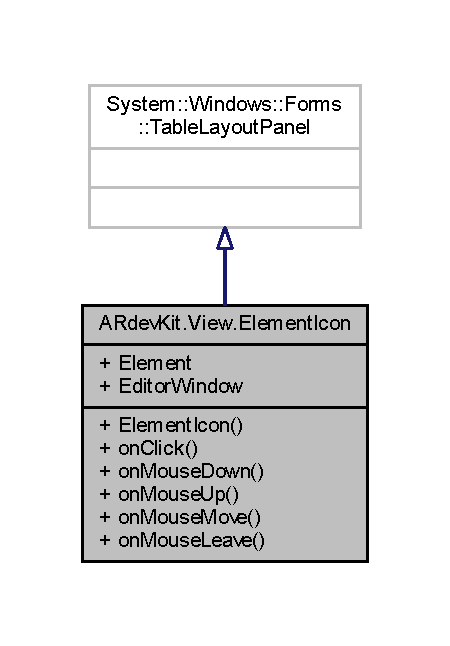
\includegraphics[width=216pt]{class_a_rdev_kit_1_1_view_1_1_element_icon__inherit__graph}
\end{center}
\end{figure}


Collaboration diagram for A\-Rdev\-Kit.\-View.\-Element\-Icon\-:
\nopagebreak
\begin{figure}[H]
\begin{center}
\leavevmode
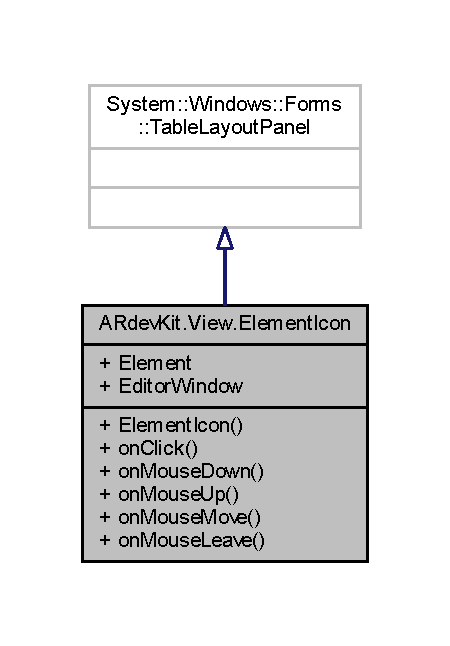
\includegraphics[width=216pt]{class_a_rdev_kit_1_1_view_1_1_element_icon__coll__graph}
\end{center}
\end{figure}
\subsection*{Public Member Functions}
\begin{DoxyCompactItemize}
\item 
\hyperlink{class_a_rdev_kit_1_1_view_1_1_element_icon_a30833a0a71c8421f5309f6c384d1ad0b}{Element\-Icon} (\hyperlink{class_a_rdev_kit_1_1_controller_1_1_editor_controller_1_1_scene_element}{Scene\-Element} element, \hyperlink{class_a_rdev_kit_1_1_editor_window}{Editor\-Window} ew)
\begin{DoxyCompactList}\small\item\em Constructor. Creates the text label and the picture\-Box and adds them to the Panel. Adds event handlers. \end{DoxyCompactList}\item 
void \hyperlink{class_a_rdev_kit_1_1_view_1_1_element_icon_a58f9a858b7276f2e84a1c5ff53c0c2ad}{on\-Click} (object sender, Event\-Args e)
\begin{DoxyCompactList}\small\item\em Raises the click event of the panel, label and picturebox. \end{DoxyCompactList}\item 
void \hyperlink{class_a_rdev_kit_1_1_view_1_1_element_icon_a74260100df10dfa4c774560c5f5eb1f1}{on\-Mouse\-Down} (object sender, Event\-Args e)
\begin{DoxyCompactList}\small\item\em Raises the mouse down event. Initiates drag\&drop. \end{DoxyCompactList}\item 
void \hyperlink{class_a_rdev_kit_1_1_view_1_1_element_icon_a8d579f67f02edc591e947fa48e0bac75}{on\-Mouse\-Up} (object sender, Event\-Args e)
\begin{DoxyCompactList}\small\item\em Raises the mouse up event. \end{DoxyCompactList}\item 
void \hyperlink{class_a_rdev_kit_1_1_view_1_1_element_icon_a2eb3b81bfad03aacdeb5321c546c48de}{on\-Mouse\-Move} (object sender, Event\-Args e)
\begin{DoxyCompactList}\small\item\em Raises the mouse move event. \end{DoxyCompactList}\item 
void \hyperlink{class_a_rdev_kit_1_1_view_1_1_element_icon_a20687dd0ecb82c3ec17341ba01256f14}{on\-Mouse\-Leave} (object sender, Event\-Args e)
\begin{DoxyCompactList}\small\item\em Raises the mouse leave event. \end{DoxyCompactList}\end{DoxyCompactItemize}
\subsection*{Properties}
\begin{DoxyCompactItemize}
\item 
\hyperlink{class_a_rdev_kit_1_1_controller_1_1_editor_controller_1_1_scene_element}{Scene\-Element} \hyperlink{class_a_rdev_kit_1_1_view_1_1_element_icon_a5d4cda78ae958d4acc7be292e6c0d99e}{Element}\hspace{0.3cm}{\ttfamily  \mbox{[}get\mbox{]}}
\begin{DoxyCompactList}\small\item\em Gets the element. \end{DoxyCompactList}\item 
\hyperlink{class_a_rdev_kit_1_1_editor_window}{Editor\-Window} \hyperlink{class_a_rdev_kit_1_1_view_1_1_element_icon_a255d6901cfa20cd8d620c675143ddddf}{Editor\-Window}\hspace{0.3cm}{\ttfamily  \mbox{[}get\mbox{]}}
\begin{DoxyCompactList}\small\item\em Gets the editor window. \end{DoxyCompactList}\end{DoxyCompactItemize}


\subsection{Detailed Description}
An element icon is used to display a registered Scene\-Element in the Scene\-Selection\-Panel. 

Robin, 14.\-01.\-2014. 

\subsection{Constructor \& Destructor Documentation}
\hypertarget{class_a_rdev_kit_1_1_view_1_1_element_icon_a30833a0a71c8421f5309f6c384d1ad0b}{\index{A\-Rdev\-Kit\-::\-View\-::\-Element\-Icon@{A\-Rdev\-Kit\-::\-View\-::\-Element\-Icon}!Element\-Icon@{Element\-Icon}}
\index{Element\-Icon@{Element\-Icon}!ARdevKit::View::ElementIcon@{A\-Rdev\-Kit\-::\-View\-::\-Element\-Icon}}
\subsubsection[{Element\-Icon}]{\setlength{\rightskip}{0pt plus 5cm}A\-Rdev\-Kit.\-View.\-Element\-Icon.\-Element\-Icon (
\begin{DoxyParamCaption}
\item[{{\bf Scene\-Element}}]{element, }
\item[{{\bf Editor\-Window}}]{ew}
\end{DoxyParamCaption}
)}}\label{class_a_rdev_kit_1_1_view_1_1_element_icon_a30833a0a71c8421f5309f6c384d1ad0b}


Constructor. Creates the text label and the picture\-Box and adds them to the Panel. Adds event handlers. 


\begin{DoxyParams}{Parameters}
{\em element} & The element.\\
\hline
{\em ew} & The ew.\\
\hline
\end{DoxyParams}


Robin, 14.\-01.\-2014. 

\subsection{Member Function Documentation}
\hypertarget{class_a_rdev_kit_1_1_view_1_1_element_icon_a58f9a858b7276f2e84a1c5ff53c0c2ad}{\index{A\-Rdev\-Kit\-::\-View\-::\-Element\-Icon@{A\-Rdev\-Kit\-::\-View\-::\-Element\-Icon}!on\-Click@{on\-Click}}
\index{on\-Click@{on\-Click}!ARdevKit::View::ElementIcon@{A\-Rdev\-Kit\-::\-View\-::\-Element\-Icon}}
\subsubsection[{on\-Click}]{\setlength{\rightskip}{0pt plus 5cm}void A\-Rdev\-Kit.\-View.\-Element\-Icon.\-on\-Click (
\begin{DoxyParamCaption}
\item[{object}]{sender, }
\item[{Event\-Args}]{e}
\end{DoxyParamCaption}
)}}\label{class_a_rdev_kit_1_1_view_1_1_element_icon_a58f9a858b7276f2e84a1c5ff53c0c2ad}


Raises the click event of the panel, label and picturebox. 

Robin, 14.\-01.\-2014. 


\begin{DoxyParams}{Parameters}
{\em sender} & Source of the event. \\
\hline
{\em e} & Event information to send to registered event handlers. \\
\hline
\end{DoxyParams}
\hypertarget{class_a_rdev_kit_1_1_view_1_1_element_icon_a74260100df10dfa4c774560c5f5eb1f1}{\index{A\-Rdev\-Kit\-::\-View\-::\-Element\-Icon@{A\-Rdev\-Kit\-::\-View\-::\-Element\-Icon}!on\-Mouse\-Down@{on\-Mouse\-Down}}
\index{on\-Mouse\-Down@{on\-Mouse\-Down}!ARdevKit::View::ElementIcon@{A\-Rdev\-Kit\-::\-View\-::\-Element\-Icon}}
\subsubsection[{on\-Mouse\-Down}]{\setlength{\rightskip}{0pt plus 5cm}void A\-Rdev\-Kit.\-View.\-Element\-Icon.\-on\-Mouse\-Down (
\begin{DoxyParamCaption}
\item[{object}]{sender, }
\item[{Event\-Args}]{e}
\end{DoxyParamCaption}
)}}\label{class_a_rdev_kit_1_1_view_1_1_element_icon_a74260100df10dfa4c774560c5f5eb1f1}


Raises the mouse down event. Initiates drag\&drop. 

Robin, 18.\-01.\-2014. 


\begin{DoxyParams}{Parameters}
{\em sender} & Source of the event. \\
\hline
{\em e} & Event information to send to registered event handlers. \\
\hline
\end{DoxyParams}
\hypertarget{class_a_rdev_kit_1_1_view_1_1_element_icon_a20687dd0ecb82c3ec17341ba01256f14}{\index{A\-Rdev\-Kit\-::\-View\-::\-Element\-Icon@{A\-Rdev\-Kit\-::\-View\-::\-Element\-Icon}!on\-Mouse\-Leave@{on\-Mouse\-Leave}}
\index{on\-Mouse\-Leave@{on\-Mouse\-Leave}!ARdevKit::View::ElementIcon@{A\-Rdev\-Kit\-::\-View\-::\-Element\-Icon}}
\subsubsection[{on\-Mouse\-Leave}]{\setlength{\rightskip}{0pt plus 5cm}void A\-Rdev\-Kit.\-View.\-Element\-Icon.\-on\-Mouse\-Leave (
\begin{DoxyParamCaption}
\item[{object}]{sender, }
\item[{Event\-Args}]{e}
\end{DoxyParamCaption}
)}}\label{class_a_rdev_kit_1_1_view_1_1_element_icon_a20687dd0ecb82c3ec17341ba01256f14}


Raises the mouse leave event. 

Robin, 19.\-01.\-2014. 


\begin{DoxyParams}{Parameters}
{\em sender} & Source of the event. \\
\hline
{\em e} & Event information to send to registered event handlers. \\
\hline
\end{DoxyParams}
\hypertarget{class_a_rdev_kit_1_1_view_1_1_element_icon_a2eb3b81bfad03aacdeb5321c546c48de}{\index{A\-Rdev\-Kit\-::\-View\-::\-Element\-Icon@{A\-Rdev\-Kit\-::\-View\-::\-Element\-Icon}!on\-Mouse\-Move@{on\-Mouse\-Move}}
\index{on\-Mouse\-Move@{on\-Mouse\-Move}!ARdevKit::View::ElementIcon@{A\-Rdev\-Kit\-::\-View\-::\-Element\-Icon}}
\subsubsection[{on\-Mouse\-Move}]{\setlength{\rightskip}{0pt plus 5cm}void A\-Rdev\-Kit.\-View.\-Element\-Icon.\-on\-Mouse\-Move (
\begin{DoxyParamCaption}
\item[{object}]{sender, }
\item[{Event\-Args}]{e}
\end{DoxyParamCaption}
)}}\label{class_a_rdev_kit_1_1_view_1_1_element_icon_a2eb3b81bfad03aacdeb5321c546c48de}


Raises the mouse move event. 

Robin, 19.\-01.\-2014. 


\begin{DoxyParams}{Parameters}
{\em sender} & Source of the event. \\
\hline
{\em e} & Event information to send to registered event handlers. \\
\hline
\end{DoxyParams}
\hypertarget{class_a_rdev_kit_1_1_view_1_1_element_icon_a8d579f67f02edc591e947fa48e0bac75}{\index{A\-Rdev\-Kit\-::\-View\-::\-Element\-Icon@{A\-Rdev\-Kit\-::\-View\-::\-Element\-Icon}!on\-Mouse\-Up@{on\-Mouse\-Up}}
\index{on\-Mouse\-Up@{on\-Mouse\-Up}!ARdevKit::View::ElementIcon@{A\-Rdev\-Kit\-::\-View\-::\-Element\-Icon}}
\subsubsection[{on\-Mouse\-Up}]{\setlength{\rightskip}{0pt plus 5cm}void A\-Rdev\-Kit.\-View.\-Element\-Icon.\-on\-Mouse\-Up (
\begin{DoxyParamCaption}
\item[{object}]{sender, }
\item[{Event\-Args}]{e}
\end{DoxyParamCaption}
)}}\label{class_a_rdev_kit_1_1_view_1_1_element_icon_a8d579f67f02edc591e947fa48e0bac75}


Raises the mouse up event. 

Robin, 19.\-01.\-2014. 


\begin{DoxyParams}{Parameters}
{\em sender} & Source of the event. \\
\hline
{\em e} & Event information to send to registered event handlers. \\
\hline
\end{DoxyParams}


\subsection{Property Documentation}
\hypertarget{class_a_rdev_kit_1_1_view_1_1_element_icon_a255d6901cfa20cd8d620c675143ddddf}{\index{A\-Rdev\-Kit\-::\-View\-::\-Element\-Icon@{A\-Rdev\-Kit\-::\-View\-::\-Element\-Icon}!Editor\-Window@{Editor\-Window}}
\index{Editor\-Window@{Editor\-Window}!ARdevKit::View::ElementIcon@{A\-Rdev\-Kit\-::\-View\-::\-Element\-Icon}}
\subsubsection[{Editor\-Window}]{\setlength{\rightskip}{0pt plus 5cm}{\bf Editor\-Window} A\-Rdev\-Kit.\-View.\-Element\-Icon.\-Editor\-Window\hspace{0.3cm}{\ttfamily [get]}}}\label{class_a_rdev_kit_1_1_view_1_1_element_icon_a255d6901cfa20cd8d620c675143ddddf}


Gets the editor window. 

The editor window. \hypertarget{class_a_rdev_kit_1_1_view_1_1_element_icon_a5d4cda78ae958d4acc7be292e6c0d99e}{\index{A\-Rdev\-Kit\-::\-View\-::\-Element\-Icon@{A\-Rdev\-Kit\-::\-View\-::\-Element\-Icon}!Element@{Element}}
\index{Element@{Element}!ARdevKit::View::ElementIcon@{A\-Rdev\-Kit\-::\-View\-::\-Element\-Icon}}
\subsubsection[{Element}]{\setlength{\rightskip}{0pt plus 5cm}{\bf Scene\-Element} A\-Rdev\-Kit.\-View.\-Element\-Icon.\-Element\hspace{0.3cm}{\ttfamily [get]}}}\label{class_a_rdev_kit_1_1_view_1_1_element_icon_a5d4cda78ae958d4acc7be292e6c0d99e}


Gets the element. 

The element. 
\hypertarget{class_a_rdev_kit_1_1_controller_1_1_editor_controller_1_1_element_selection_controller}{\section{A\-Rdev\-Kit.\-Controller.\-Editor\-Controller.\-Element\-Selection\-Controller Class Reference}
\label{class_a_rdev_kit_1_1_controller_1_1_editor_controller_1_1_element_selection_controller}\index{A\-Rdev\-Kit.\-Controller.\-Editor\-Controller.\-Element\-Selection\-Controller@{A\-Rdev\-Kit.\-Controller.\-Editor\-Controller.\-Element\-Selection\-Controller}}
}


The \hyperlink{class_a_rdev_kit_1_1_controller_1_1_editor_controller_1_1_element_selection_controller}{Element\-Selection\-Controller} is used to controll the section of the U\-I,  




Collaboration diagram for A\-Rdev\-Kit.\-Controller.\-Editor\-Controller.\-Element\-Selection\-Controller\-:
\nopagebreak
\begin{figure}[H]
\begin{center}
\leavevmode
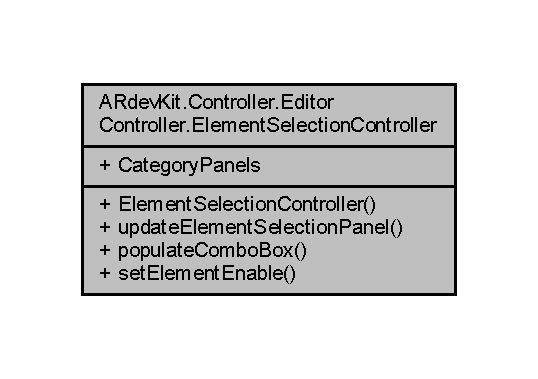
\includegraphics[width=258pt]{class_a_rdev_kit_1_1_controller_1_1_editor_controller_1_1_element_selection_controller__coll__graph}
\end{center}
\end{figure}
\subsection*{Public Member Functions}
\begin{DoxyCompactItemize}
\item 
\hyperlink{class_a_rdev_kit_1_1_controller_1_1_editor_controller_1_1_element_selection_controller_af47cc4cd03ff1da41dd787719e70f4cd}{Element\-Selection\-Controller} (\hyperlink{class_a_rdev_kit_1_1_editor_window}{Editor\-Window} ew)
\begin{DoxyCompactList}\small\item\em Constructor. \end{DoxyCompactList}\item 
void \hyperlink{class_a_rdev_kit_1_1_controller_1_1_editor_controller_1_1_element_selection_controller_a8901ac3bab63f9b4f38f5ba2b86a86d8}{update\-Element\-Selection\-Panel} ()
\begin{DoxyCompactList}\small\item\em Updates the Element\-Selection\-Panel. \end{DoxyCompactList}\item 
void \hyperlink{class_a_rdev_kit_1_1_controller_1_1_editor_controller_1_1_element_selection_controller_a1bf985716c260e5c312d59a342c4fcb1}{populate\-Combo\-Box} ()
\begin{DoxyCompactList}\small\item\em Adds the Scene\-Element\-Categories to the Combo\-Box of the Element\-Selection\-Panel. \end{DoxyCompactList}\item 
void \hyperlink{class_a_rdev_kit_1_1_controller_1_1_editor_controller_1_1_element_selection_controller_a470d43f1c3fe742fcf7ff5f8f5675819}{set\-Element\-Enable} (Type element, Boolean enable)
\begin{DoxyCompactList}\small\item\em Disables or enables the given element in the Element Selection Panel. \end{DoxyCompactList}\end{DoxyCompactItemize}
\subsection*{Properties}
\begin{DoxyCompactItemize}
\item 
List$<$ \hyperlink{class_a_rdev_kit_1_1_view_1_1_scene_element_category_panel}{Scene\-Element\-Category\-Panel} $>$ \hyperlink{class_a_rdev_kit_1_1_controller_1_1_editor_controller_1_1_element_selection_controller_a23dae11ee466555e6be598481a3459f2}{Category\-Panels}\hspace{0.3cm}{\ttfamily  \mbox{[}get, set\mbox{]}}
\begin{DoxyCompactList}\small\item\em Gets or sets the category panels. \end{DoxyCompactList}\end{DoxyCompactItemize}


\subsection{Detailed Description}
The \hyperlink{class_a_rdev_kit_1_1_controller_1_1_editor_controller_1_1_element_selection_controller}{Element\-Selection\-Controller} is used to controll the section of the U\-I, 



\subsection{Constructor \& Destructor Documentation}
\hypertarget{class_a_rdev_kit_1_1_controller_1_1_editor_controller_1_1_element_selection_controller_af47cc4cd03ff1da41dd787719e70f4cd}{\index{A\-Rdev\-Kit\-::\-Controller\-::\-Editor\-Controller\-::\-Element\-Selection\-Controller@{A\-Rdev\-Kit\-::\-Controller\-::\-Editor\-Controller\-::\-Element\-Selection\-Controller}!Element\-Selection\-Controller@{Element\-Selection\-Controller}}
\index{Element\-Selection\-Controller@{Element\-Selection\-Controller}!ARdevKit::Controller::EditorController::ElementSelectionController@{A\-Rdev\-Kit\-::\-Controller\-::\-Editor\-Controller\-::\-Element\-Selection\-Controller}}
\subsubsection[{Element\-Selection\-Controller}]{\setlength{\rightskip}{0pt plus 5cm}A\-Rdev\-Kit.\-Controller.\-Editor\-Controller.\-Element\-Selection\-Controller.\-Element\-Selection\-Controller (
\begin{DoxyParamCaption}
\item[{{\bf Editor\-Window}}]{ew}
\end{DoxyParamCaption}
)}}\label{class_a_rdev_kit_1_1_controller_1_1_editor_controller_1_1_element_selection_controller_af47cc4cd03ff1da41dd787719e70f4cd}


Constructor. 

Lizzard, 1/13/2014. 


\begin{DoxyParams}{Parameters}
{\em ew} & The Editor Window. \\
\hline
\end{DoxyParams}


\subsection{Member Function Documentation}
\hypertarget{class_a_rdev_kit_1_1_controller_1_1_editor_controller_1_1_element_selection_controller_a1bf985716c260e5c312d59a342c4fcb1}{\index{A\-Rdev\-Kit\-::\-Controller\-::\-Editor\-Controller\-::\-Element\-Selection\-Controller@{A\-Rdev\-Kit\-::\-Controller\-::\-Editor\-Controller\-::\-Element\-Selection\-Controller}!populate\-Combo\-Box@{populate\-Combo\-Box}}
\index{populate\-Combo\-Box@{populate\-Combo\-Box}!ARdevKit::Controller::EditorController::ElementSelectionController@{A\-Rdev\-Kit\-::\-Controller\-::\-Editor\-Controller\-::\-Element\-Selection\-Controller}}
\subsubsection[{populate\-Combo\-Box}]{\setlength{\rightskip}{0pt plus 5cm}void A\-Rdev\-Kit.\-Controller.\-Editor\-Controller.\-Element\-Selection\-Controller.\-populate\-Combo\-Box (
\begin{DoxyParamCaption}
{}
\end{DoxyParamCaption}
)}}\label{class_a_rdev_kit_1_1_controller_1_1_editor_controller_1_1_element_selection_controller_a1bf985716c260e5c312d59a342c4fcb1}


Adds the Scene\-Element\-Categories to the Combo\-Box of the Element\-Selection\-Panel. 

Lizzard, 1/13/2014. \hypertarget{class_a_rdev_kit_1_1_controller_1_1_editor_controller_1_1_element_selection_controller_a470d43f1c3fe742fcf7ff5f8f5675819}{\index{A\-Rdev\-Kit\-::\-Controller\-::\-Editor\-Controller\-::\-Element\-Selection\-Controller@{A\-Rdev\-Kit\-::\-Controller\-::\-Editor\-Controller\-::\-Element\-Selection\-Controller}!set\-Element\-Enable@{set\-Element\-Enable}}
\index{set\-Element\-Enable@{set\-Element\-Enable}!ARdevKit::Controller::EditorController::ElementSelectionController@{A\-Rdev\-Kit\-::\-Controller\-::\-Editor\-Controller\-::\-Element\-Selection\-Controller}}
\subsubsection[{set\-Element\-Enable}]{\setlength{\rightskip}{0pt plus 5cm}void A\-Rdev\-Kit.\-Controller.\-Editor\-Controller.\-Element\-Selection\-Controller.\-set\-Element\-Enable (
\begin{DoxyParamCaption}
\item[{Type}]{element, }
\item[{Boolean}]{enable}
\end{DoxyParamCaption}
)}}\label{class_a_rdev_kit_1_1_controller_1_1_editor_controller_1_1_element_selection_controller_a470d43f1c3fe742fcf7ff5f8f5675819}


Disables or enables the given element in the Element Selection Panel. 

Robin, 19.\-01.\-2014. 


\begin{DoxyParams}{Parameters}
{\em element} & The element to disable or enable. Example\-: typeof(\-I\-D\-Marker) \\
\hline
{\em enable} & Whether the element should be dis or enabled. \\
\hline
\end{DoxyParams}
\hypertarget{class_a_rdev_kit_1_1_controller_1_1_editor_controller_1_1_element_selection_controller_a8901ac3bab63f9b4f38f5ba2b86a86d8}{\index{A\-Rdev\-Kit\-::\-Controller\-::\-Editor\-Controller\-::\-Element\-Selection\-Controller@{A\-Rdev\-Kit\-::\-Controller\-::\-Editor\-Controller\-::\-Element\-Selection\-Controller}!update\-Element\-Selection\-Panel@{update\-Element\-Selection\-Panel}}
\index{update\-Element\-Selection\-Panel@{update\-Element\-Selection\-Panel}!ARdevKit::Controller::EditorController::ElementSelectionController@{A\-Rdev\-Kit\-::\-Controller\-::\-Editor\-Controller\-::\-Element\-Selection\-Controller}}
\subsubsection[{update\-Element\-Selection\-Panel}]{\setlength{\rightskip}{0pt plus 5cm}void A\-Rdev\-Kit.\-Controller.\-Editor\-Controller.\-Element\-Selection\-Controller.\-update\-Element\-Selection\-Panel (
\begin{DoxyParamCaption}
{}
\end{DoxyParamCaption}
)}}\label{class_a_rdev_kit_1_1_controller_1_1_editor_controller_1_1_element_selection_controller_a8901ac3bab63f9b4f38f5ba2b86a86d8}


Updates the Element\-Selection\-Panel. 

Lizzard, 1/13/2014. 

\subsection{Property Documentation}
\hypertarget{class_a_rdev_kit_1_1_controller_1_1_editor_controller_1_1_element_selection_controller_a23dae11ee466555e6be598481a3459f2}{\index{A\-Rdev\-Kit\-::\-Controller\-::\-Editor\-Controller\-::\-Element\-Selection\-Controller@{A\-Rdev\-Kit\-::\-Controller\-::\-Editor\-Controller\-::\-Element\-Selection\-Controller}!Category\-Panels@{Category\-Panels}}
\index{Category\-Panels@{Category\-Panels}!ARdevKit::Controller::EditorController::ElementSelectionController@{A\-Rdev\-Kit\-::\-Controller\-::\-Editor\-Controller\-::\-Element\-Selection\-Controller}}
\subsubsection[{Category\-Panels}]{\setlength{\rightskip}{0pt plus 5cm}List$<${\bf Scene\-Element\-Category\-Panel}$>$ A\-Rdev\-Kit.\-Controller.\-Editor\-Controller.\-Element\-Selection\-Controller.\-Category\-Panels\hspace{0.3cm}{\ttfamily [get]}, {\ttfamily [set]}}}\label{class_a_rdev_kit_1_1_controller_1_1_editor_controller_1_1_element_selection_controller_a23dae11ee466555e6be598481a3459f2}


Gets or sets the category panels. 

The category panels. 
\hypertarget{class_a_rdev_kit_1_1_controller_1_1_project_controller_1_1_export_visitor}{\section{A\-Rdev\-Kit.\-Controller.\-Project\-Controller.\-Export\-Visitor Class Reference}
\label{class_a_rdev_kit_1_1_controller_1_1_project_controller_1_1_export_visitor}\index{A\-Rdev\-Kit.\-Controller.\-Project\-Controller.\-Export\-Visitor@{A\-Rdev\-Kit.\-Controller.\-Project\-Controller.\-Export\-Visitor}}
}


An \hyperlink{class_a_rdev_kit_1_1_controller_1_1_project_controller_1_1_export_visitor}{Export\-Visitor} is an \hyperlink{class_a_rdev_kit_1_1_controller_1_1_project_controller_1_1_abstract_project_visitor}{Abstract\-Project\-Visitor} which exports the project to the path defined in Project so that it is readable by the player.  




Inheritance diagram for A\-Rdev\-Kit.\-Controller.\-Project\-Controller.\-Export\-Visitor\-:
\nopagebreak
\begin{figure}[H]
\begin{center}
\leavevmode
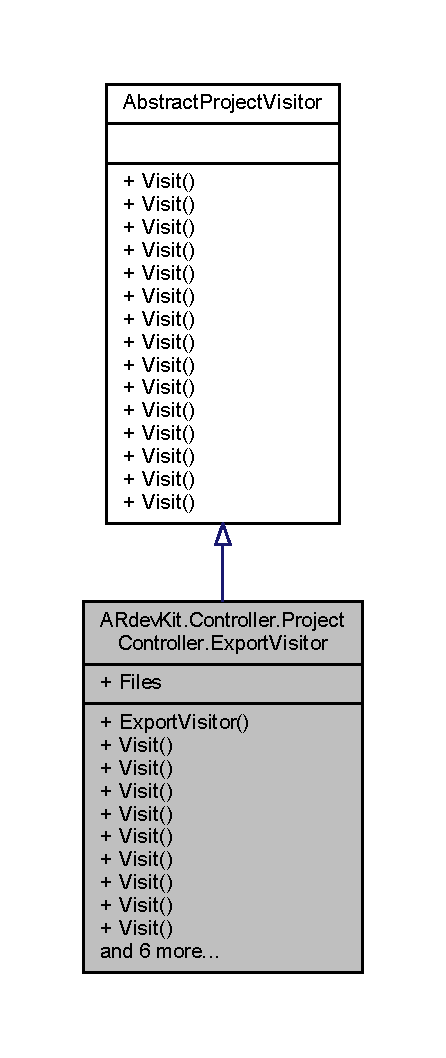
\includegraphics[width=214pt]{class_a_rdev_kit_1_1_controller_1_1_project_controller_1_1_export_visitor__inherit__graph}
\end{center}
\end{figure}


Collaboration diagram for A\-Rdev\-Kit.\-Controller.\-Project\-Controller.\-Export\-Visitor\-:
\nopagebreak
\begin{figure}[H]
\begin{center}
\leavevmode
\includegraphics[width=214pt]{class_a_rdev_kit_1_1_controller_1_1_project_controller_1_1_export_visitor__coll__graph}
\end{center}
\end{figure}
\subsection*{Public Member Functions}
\begin{DoxyCompactItemize}
\item 
\hyperlink{class_a_rdev_kit_1_1_controller_1_1_project_controller_1_1_export_visitor_a1e1a8bc6cbba6dca7ade01cec777b4c5}{Export\-Visitor} ()
\begin{DoxyCompactList}\small\item\em Default constructor \end{DoxyCompactList}\item 
override void \hyperlink{class_a_rdev_kit_1_1_controller_1_1_project_controller_1_1_export_visitor_a4d2802913e6ccb1a24e53c642d1b1cff}{Visit} (\hyperlink{class_a_rdev_kit_1_1_model_1_1_project_1_1_custom_user_event}{Custom\-User\-Event} cue)
\begin{DoxyCompactList}\small\item\em Visits the given Custom\-User\-Event \end{DoxyCompactList}\item 
override void \hyperlink{class_a_rdev_kit_1_1_controller_1_1_project_controller_1_1_export_visitor_a190039e5dd86df278c99cfacedac3b63}{Visit} (\hyperlink{class_a_rdev_kit_1_1_model_1_1_project_1_1_video_augmentation}{Video\-Augmentation} video)
\begin{DoxyCompactList}\small\item\em Visits the given Video\-Augmentation \end{DoxyCompactList}\item 
override void \hyperlink{class_a_rdev_kit_1_1_controller_1_1_project_controller_1_1_export_visitor_a68256626e59d84b43153e95697ed1e3a}{Visit} (\hyperlink{class_a_rdev_kit_1_1_model_1_1_project_1_1_image_augmentation}{Image\-Augmentation} image)
\begin{DoxyCompactList}\small\item\em Visits the given Image\-Augmentation. \end{DoxyCompactList}\item 
override void \hyperlink{class_a_rdev_kit_1_1_controller_1_1_project_controller_1_1_export_visitor_a0e04a0743609a16eb7c872427755249e}{Visit} (\hyperlink{class_a_rdev_kit_1_1_model_1_1_project_1_1_chart}{Chart} chart)
\begin{DoxyCompactList}\small\item\em Visits the given Chart. \end{DoxyCompactList}\item 
override void \hyperlink{class_a_rdev_kit_1_1_controller_1_1_project_controller_1_1_export_visitor_a54481877bd367164a17916ff32f8da09}{Visit} (\hyperlink{class_a_rdev_kit_1_1_model_1_1_project_1_1_db_source}{Db\-Source} source)
\begin{DoxyCompactList}\small\item\em Visits the given Db\-Source. \end{DoxyCompactList}\item 
override void \hyperlink{class_a_rdev_kit_1_1_controller_1_1_project_controller_1_1_export_visitor_a078a2d0fef2fa5db4b6adcf4be50debe}{Visit} (\hyperlink{class_a_rdev_kit_1_1_model_1_1_project_1_1_file_source}{File\-Source} source)
\begin{DoxyCompactList}\small\item\em Visits the given File\-Source. \end{DoxyCompactList}\item 
override void \hyperlink{class_a_rdev_kit_1_1_controller_1_1_project_controller_1_1_export_visitor_aae0293dd695393b0037fb62f0f5a1d28}{Visit} (\hyperlink{class_a_rdev_kit_1_1_model_1_1_project_1_1_markerless_fuser}{Markerless\-Fuser} markerless\-Fuser)
\begin{DoxyCompactList}\small\item\em Visits the given Markerless\-Fuser. \end{DoxyCompactList}\item 
override void \hyperlink{class_a_rdev_kit_1_1_controller_1_1_project_controller_1_1_export_visitor_abf7c8bbff198ee8af664232c2fa394cb}{Visit} (\hyperlink{class_a_rdev_kit_1_1_model_1_1_project_1_1_markerless_sensor}{Markerless\-Sensor} markerless\-Sensor)
\begin{DoxyCompactList}\small\item\em Visits the given Markerless\-Sensor. \end{DoxyCompactList}\item 
override void \hyperlink{class_a_rdev_kit_1_1_controller_1_1_project_controller_1_1_export_visitor_a315b092cbd6a936b67d3ea690920bd95}{Visit} (\hyperlink{class_a_rdev_kit_1_1_model_1_1_project_1_1_marker_fuser}{Marker\-Fuser} marker\-Fuser)
\begin{DoxyCompactList}\small\item\em Visits the given Marker\-Fuser. \end{DoxyCompactList}\item 
override void \hyperlink{class_a_rdev_kit_1_1_controller_1_1_project_controller_1_1_export_visitor_a567d0ff197539453cc2c34b11f12ad59}{Visit} (\hyperlink{class_a_rdev_kit_1_1_model_1_1_project_1_1_picture_marker_sensor}{Picture\-Marker\-Sensor} picture\-Marker\-Sensor)
\begin{DoxyCompactList}\small\item\em Visits the given Picture\-Marker\-Sensor. \end{DoxyCompactList}\item 
override void \hyperlink{class_a_rdev_kit_1_1_controller_1_1_project_controller_1_1_export_visitor_a6ba67134957206067b97c6ebba5a9c8a}{Visit} (\hyperlink{class_a_rdev_kit_1_1_model_1_1_project_1_1_image_trackable}{Image\-Trackable} image)
\begin{DoxyCompactList}\small\item\em Visits the given Image. \end{DoxyCompactList}\item 
override void \hyperlink{class_a_rdev_kit_1_1_controller_1_1_project_controller_1_1_export_visitor_a384b6fc84602fd29bedff296b083b3a0}{Visit} (\hyperlink{class_a_rdev_kit_1_1_model_1_1_project_1_1_picture_marker}{Picture\-Marker} picture\-Marker)
\begin{DoxyCompactList}\small\item\em Visits the given Picture\-Marker. \end{DoxyCompactList}\item 
override void \hyperlink{class_a_rdev_kit_1_1_controller_1_1_project_controller_1_1_export_visitor_a0e82718aa35b9bff19cd6db0b33f3d5c}{Visit} (\hyperlink{class_a_rdev_kit_1_1_model_1_1_project_1_1_marker_sensor}{Marker\-Sensor} id\-Marker\-Sensor)
\begin{DoxyCompactList}\small\item\em Visits the given Marker\-Sensor. \end{DoxyCompactList}\item 
override void \hyperlink{class_a_rdev_kit_1_1_controller_1_1_project_controller_1_1_export_visitor_aa4ad67b0cb408d8ec6aaf48906f1e5b3}{Visit} (\hyperlink{class_a_rdev_kit_1_1_model_1_1_project_1_1_i_d_marker}{I\-D\-Marker} id\-Marker)
\begin{DoxyCompactList}\small\item\em Visits the given I\-D\-Marker. \end{DoxyCompactList}\item 
override void \hyperlink{class_a_rdev_kit_1_1_controller_1_1_project_controller_1_1_export_visitor_ad58774c6778421b6bf85a6c70029a3d9}{Visit} (\hyperlink{class_a_rdev_kit_1_1_model_1_1_project_1_1_project}{Project} p)
\begin{DoxyCompactList}\small\item\em Visits the given Project. \end{DoxyCompactList}\end{DoxyCompactItemize}
\subsection*{Properties}
\begin{DoxyCompactItemize}
\item 
List$<$ \hyperlink{class_a_rdev_kit_1_1_model_1_1_project_1_1_file_1_1_abstract_file}{Abstract\-File} $>$ \hyperlink{class_a_rdev_kit_1_1_controller_1_1_project_controller_1_1_export_visitor_ac241f50a7b72f0cf3dc5b77c42a6a71b}{Files}\hspace{0.3cm}{\ttfamily  \mbox{[}get, set\mbox{]}}
\begin{DoxyCompactList}\small\item\em Gets or sets the Abstract\-Files created by the export visitor. \end{DoxyCompactList}\end{DoxyCompactItemize}


\subsection{Detailed Description}
An \hyperlink{class_a_rdev_kit_1_1_controller_1_1_project_controller_1_1_export_visitor}{Export\-Visitor} is an \hyperlink{class_a_rdev_kit_1_1_controller_1_1_project_controller_1_1_abstract_project_visitor}{Abstract\-Project\-Visitor} which exports the project to the path defined in Project so that it is readable by the player. 

Imanuel, 15.\-01.\-2014. 

\subsection{Constructor \& Destructor Documentation}
\hypertarget{class_a_rdev_kit_1_1_controller_1_1_project_controller_1_1_export_visitor_a1e1a8bc6cbba6dca7ade01cec777b4c5}{\index{A\-Rdev\-Kit\-::\-Controller\-::\-Project\-Controller\-::\-Export\-Visitor@{A\-Rdev\-Kit\-::\-Controller\-::\-Project\-Controller\-::\-Export\-Visitor}!Export\-Visitor@{Export\-Visitor}}
\index{Export\-Visitor@{Export\-Visitor}!ARdevKit::Controller::ProjectController::ExportVisitor@{A\-Rdev\-Kit\-::\-Controller\-::\-Project\-Controller\-::\-Export\-Visitor}}
\subsubsection[{Export\-Visitor}]{\setlength{\rightskip}{0pt plus 5cm}A\-Rdev\-Kit.\-Controller.\-Project\-Controller.\-Export\-Visitor.\-Export\-Visitor (
\begin{DoxyParamCaption}
{}
\end{DoxyParamCaption}
)}}\label{class_a_rdev_kit_1_1_controller_1_1_project_controller_1_1_export_visitor_a1e1a8bc6cbba6dca7ade01cec777b4c5}


Default constructor 



\subsection{Member Function Documentation}
\hypertarget{class_a_rdev_kit_1_1_controller_1_1_project_controller_1_1_export_visitor_a4d2802913e6ccb1a24e53c642d1b1cff}{\index{A\-Rdev\-Kit\-::\-Controller\-::\-Project\-Controller\-::\-Export\-Visitor@{A\-Rdev\-Kit\-::\-Controller\-::\-Project\-Controller\-::\-Export\-Visitor}!Visit@{Visit}}
\index{Visit@{Visit}!ARdevKit::Controller::ProjectController::ExportVisitor@{A\-Rdev\-Kit\-::\-Controller\-::\-Project\-Controller\-::\-Export\-Visitor}}
\subsubsection[{Visit}]{\setlength{\rightskip}{0pt plus 5cm}override void A\-Rdev\-Kit.\-Controller.\-Project\-Controller.\-Export\-Visitor.\-Visit (
\begin{DoxyParamCaption}
\item[{{\bf Custom\-User\-Event}}]{cue}
\end{DoxyParamCaption}
)\hspace{0.3cm}{\ttfamily [virtual]}}}\label{class_a_rdev_kit_1_1_controller_1_1_project_controller_1_1_export_visitor_a4d2802913e6ccb1a24e53c642d1b1cff}


Visits the given Custom\-User\-Event 


\begin{DoxyParams}{Parameters}
{\em cue} & The custom\-User\-Event\\
\hline
\end{DoxyParams}


Implements \hyperlink{class_a_rdev_kit_1_1_controller_1_1_project_controller_1_1_abstract_project_visitor_aafdd79d5f00d223cb7a5269344b55e8d}{A\-Rdev\-Kit.\-Controller.\-Project\-Controller.\-Abstract\-Project\-Visitor}.

\hypertarget{class_a_rdev_kit_1_1_controller_1_1_project_controller_1_1_export_visitor_a190039e5dd86df278c99cfacedac3b63}{\index{A\-Rdev\-Kit\-::\-Controller\-::\-Project\-Controller\-::\-Export\-Visitor@{A\-Rdev\-Kit\-::\-Controller\-::\-Project\-Controller\-::\-Export\-Visitor}!Visit@{Visit}}
\index{Visit@{Visit}!ARdevKit::Controller::ProjectController::ExportVisitor@{A\-Rdev\-Kit\-::\-Controller\-::\-Project\-Controller\-::\-Export\-Visitor}}
\subsubsection[{Visit}]{\setlength{\rightskip}{0pt plus 5cm}override void A\-Rdev\-Kit.\-Controller.\-Project\-Controller.\-Export\-Visitor.\-Visit (
\begin{DoxyParamCaption}
\item[{{\bf Video\-Augmentation}}]{video}
\end{DoxyParamCaption}
)\hspace{0.3cm}{\ttfamily [virtual]}}}\label{class_a_rdev_kit_1_1_controller_1_1_project_controller_1_1_export_visitor_a190039e5dd86df278c99cfacedac3b63}


Visits the given Video\-Augmentation 


\begin{DoxyParams}{Parameters}
{\em video} & The video\\
\hline
\end{DoxyParams}


Implements \hyperlink{class_a_rdev_kit_1_1_controller_1_1_project_controller_1_1_abstract_project_visitor_afd227a5cdb38cbfe2bb88ca22a5adf56}{A\-Rdev\-Kit.\-Controller.\-Project\-Controller.\-Abstract\-Project\-Visitor}.

\hypertarget{class_a_rdev_kit_1_1_controller_1_1_project_controller_1_1_export_visitor_a68256626e59d84b43153e95697ed1e3a}{\index{A\-Rdev\-Kit\-::\-Controller\-::\-Project\-Controller\-::\-Export\-Visitor@{A\-Rdev\-Kit\-::\-Controller\-::\-Project\-Controller\-::\-Export\-Visitor}!Visit@{Visit}}
\index{Visit@{Visit}!ARdevKit::Controller::ProjectController::ExportVisitor@{A\-Rdev\-Kit\-::\-Controller\-::\-Project\-Controller\-::\-Export\-Visitor}}
\subsubsection[{Visit}]{\setlength{\rightskip}{0pt plus 5cm}override void A\-Rdev\-Kit.\-Controller.\-Project\-Controller.\-Export\-Visitor.\-Visit (
\begin{DoxyParamCaption}
\item[{{\bf Image\-Augmentation}}]{image}
\end{DoxyParamCaption}
)\hspace{0.3cm}{\ttfamily [virtual]}}}\label{class_a_rdev_kit_1_1_controller_1_1_project_controller_1_1_export_visitor_a68256626e59d84b43153e95697ed1e3a}


Visits the given Image\-Augmentation. 

Imanuel, 17.\-01.\-2014. 


\begin{DoxyParams}{Parameters}
{\em image} & The image. \\
\hline
\end{DoxyParams}


Implements \hyperlink{class_a_rdev_kit_1_1_controller_1_1_project_controller_1_1_abstract_project_visitor_a9f0a4ed7ac360a201255c1ed37759bee}{A\-Rdev\-Kit.\-Controller.\-Project\-Controller.\-Abstract\-Project\-Visitor}.

\hypertarget{class_a_rdev_kit_1_1_controller_1_1_project_controller_1_1_export_visitor_a0e04a0743609a16eb7c872427755249e}{\index{A\-Rdev\-Kit\-::\-Controller\-::\-Project\-Controller\-::\-Export\-Visitor@{A\-Rdev\-Kit\-::\-Controller\-::\-Project\-Controller\-::\-Export\-Visitor}!Visit@{Visit}}
\index{Visit@{Visit}!ARdevKit::Controller::ProjectController::ExportVisitor@{A\-Rdev\-Kit\-::\-Controller\-::\-Project\-Controller\-::\-Export\-Visitor}}
\subsubsection[{Visit}]{\setlength{\rightskip}{0pt plus 5cm}override void A\-Rdev\-Kit.\-Controller.\-Project\-Controller.\-Export\-Visitor.\-Visit (
\begin{DoxyParamCaption}
\item[{{\bf Chart}}]{chart}
\end{DoxyParamCaption}
)\hspace{0.3cm}{\ttfamily [virtual]}}}\label{class_a_rdev_kit_1_1_controller_1_1_project_controller_1_1_export_visitor_a0e04a0743609a16eb7c872427755249e}


Visits the given Chart. 

Imanuel, 17.\-01.\-2014. 


\begin{DoxyParams}{Parameters}
{\em chart} & The bar graph. \\
\hline
\end{DoxyParams}


Implements \hyperlink{class_a_rdev_kit_1_1_controller_1_1_project_controller_1_1_abstract_project_visitor_afc567731ac7e98ef86c2d26c5f22b4d8}{A\-Rdev\-Kit.\-Controller.\-Project\-Controller.\-Abstract\-Project\-Visitor}.

\hypertarget{class_a_rdev_kit_1_1_controller_1_1_project_controller_1_1_export_visitor_a54481877bd367164a17916ff32f8da09}{\index{A\-Rdev\-Kit\-::\-Controller\-::\-Project\-Controller\-::\-Export\-Visitor@{A\-Rdev\-Kit\-::\-Controller\-::\-Project\-Controller\-::\-Export\-Visitor}!Visit@{Visit}}
\index{Visit@{Visit}!ARdevKit::Controller::ProjectController::ExportVisitor@{A\-Rdev\-Kit\-::\-Controller\-::\-Project\-Controller\-::\-Export\-Visitor}}
\subsubsection[{Visit}]{\setlength{\rightskip}{0pt plus 5cm}override void A\-Rdev\-Kit.\-Controller.\-Project\-Controller.\-Export\-Visitor.\-Visit (
\begin{DoxyParamCaption}
\item[{{\bf Db\-Source}}]{source}
\end{DoxyParamCaption}
)\hspace{0.3cm}{\ttfamily [virtual]}}}\label{class_a_rdev_kit_1_1_controller_1_1_project_controller_1_1_export_visitor_a54481877bd367164a17916ff32f8da09}


Visits the given Db\-Source. 

Imanuel, 17.\-01.\-2014. 


\begin{DoxyExceptions}{Exceptions}
{\em Not\-Implemented\-Exception} & Thrown when the requested operation is unimplemented. \\
\hline
\end{DoxyExceptions}



\begin{DoxyParams}{Parameters}
{\em source} & Source for the. \\
\hline
\end{DoxyParams}


Implements \hyperlink{class_a_rdev_kit_1_1_controller_1_1_project_controller_1_1_abstract_project_visitor_ae89191e9e36e1de0ca8b2a68aa20c13f}{A\-Rdev\-Kit.\-Controller.\-Project\-Controller.\-Abstract\-Project\-Visitor}.

\hypertarget{class_a_rdev_kit_1_1_controller_1_1_project_controller_1_1_export_visitor_a078a2d0fef2fa5db4b6adcf4be50debe}{\index{A\-Rdev\-Kit\-::\-Controller\-::\-Project\-Controller\-::\-Export\-Visitor@{A\-Rdev\-Kit\-::\-Controller\-::\-Project\-Controller\-::\-Export\-Visitor}!Visit@{Visit}}
\index{Visit@{Visit}!ARdevKit::Controller::ProjectController::ExportVisitor@{A\-Rdev\-Kit\-::\-Controller\-::\-Project\-Controller\-::\-Export\-Visitor}}
\subsubsection[{Visit}]{\setlength{\rightskip}{0pt plus 5cm}override void A\-Rdev\-Kit.\-Controller.\-Project\-Controller.\-Export\-Visitor.\-Visit (
\begin{DoxyParamCaption}
\item[{{\bf File\-Source}}]{source}
\end{DoxyParamCaption}
)\hspace{0.3cm}{\ttfamily [virtual]}}}\label{class_a_rdev_kit_1_1_controller_1_1_project_controller_1_1_export_visitor_a078a2d0fef2fa5db4b6adcf4be50debe}


Visits the given File\-Source. 

Imanuel, 23.\-01.\-2014. 


\begin{DoxyExceptions}{Exceptions}
{\em Not\-Implemented\-Exception} & Thrown when the requested operation is unimplemented. \\
\hline
\end{DoxyExceptions}



\begin{DoxyParams}{Parameters}
{\em source} & Source for the Abstract\-Dynamic2\-D\-Augmentation. \\
\hline
\end{DoxyParams}


Implements \hyperlink{class_a_rdev_kit_1_1_controller_1_1_project_controller_1_1_abstract_project_visitor_a57f6cd714839140a46e4d68a29c65287}{A\-Rdev\-Kit.\-Controller.\-Project\-Controller.\-Abstract\-Project\-Visitor}.

\hypertarget{class_a_rdev_kit_1_1_controller_1_1_project_controller_1_1_export_visitor_aae0293dd695393b0037fb62f0f5a1d28}{\index{A\-Rdev\-Kit\-::\-Controller\-::\-Project\-Controller\-::\-Export\-Visitor@{A\-Rdev\-Kit\-::\-Controller\-::\-Project\-Controller\-::\-Export\-Visitor}!Visit@{Visit}}
\index{Visit@{Visit}!ARdevKit::Controller::ProjectController::ExportVisitor@{A\-Rdev\-Kit\-::\-Controller\-::\-Project\-Controller\-::\-Export\-Visitor}}
\subsubsection[{Visit}]{\setlength{\rightskip}{0pt plus 5cm}override void A\-Rdev\-Kit.\-Controller.\-Project\-Controller.\-Export\-Visitor.\-Visit (
\begin{DoxyParamCaption}
\item[{{\bf Markerless\-Fuser}}]{markerless\-Fuser}
\end{DoxyParamCaption}
)\hspace{0.3cm}{\ttfamily [virtual]}}}\label{class_a_rdev_kit_1_1_controller_1_1_project_controller_1_1_export_visitor_aae0293dd695393b0037fb62f0f5a1d28}


Visits the given Markerless\-Fuser. 

Imanuel, 17.\-01.\-2014. 


\begin{DoxyParams}{Parameters}
{\em markerless\-Fuser} & The markerless fuser. \\
\hline
\end{DoxyParams}


Implements \hyperlink{class_a_rdev_kit_1_1_controller_1_1_project_controller_1_1_abstract_project_visitor_a81cd1e82508e62b748421a2e3f128fa2}{A\-Rdev\-Kit.\-Controller.\-Project\-Controller.\-Abstract\-Project\-Visitor}.

\hypertarget{class_a_rdev_kit_1_1_controller_1_1_project_controller_1_1_export_visitor_abf7c8bbff198ee8af664232c2fa394cb}{\index{A\-Rdev\-Kit\-::\-Controller\-::\-Project\-Controller\-::\-Export\-Visitor@{A\-Rdev\-Kit\-::\-Controller\-::\-Project\-Controller\-::\-Export\-Visitor}!Visit@{Visit}}
\index{Visit@{Visit}!ARdevKit::Controller::ProjectController::ExportVisitor@{A\-Rdev\-Kit\-::\-Controller\-::\-Project\-Controller\-::\-Export\-Visitor}}
\subsubsection[{Visit}]{\setlength{\rightskip}{0pt plus 5cm}override void A\-Rdev\-Kit.\-Controller.\-Project\-Controller.\-Export\-Visitor.\-Visit (
\begin{DoxyParamCaption}
\item[{{\bf Markerless\-Sensor}}]{markerless\-Sensor}
\end{DoxyParamCaption}
)\hspace{0.3cm}{\ttfamily [virtual]}}}\label{class_a_rdev_kit_1_1_controller_1_1_project_controller_1_1_export_visitor_abf7c8bbff198ee8af664232c2fa394cb}


Visits the given Markerless\-Sensor. 

Imanuel, 17.\-01.\-2014. 


\begin{DoxyParams}{Parameters}
{\em markerless\-Sensor} & The markerless sensor. \\
\hline
\end{DoxyParams}


Implements \hyperlink{class_a_rdev_kit_1_1_controller_1_1_project_controller_1_1_abstract_project_visitor_ab954e7db5de1aafc57e082020eba3f3b}{A\-Rdev\-Kit.\-Controller.\-Project\-Controller.\-Abstract\-Project\-Visitor}.

\hypertarget{class_a_rdev_kit_1_1_controller_1_1_project_controller_1_1_export_visitor_a315b092cbd6a936b67d3ea690920bd95}{\index{A\-Rdev\-Kit\-::\-Controller\-::\-Project\-Controller\-::\-Export\-Visitor@{A\-Rdev\-Kit\-::\-Controller\-::\-Project\-Controller\-::\-Export\-Visitor}!Visit@{Visit}}
\index{Visit@{Visit}!ARdevKit::Controller::ProjectController::ExportVisitor@{A\-Rdev\-Kit\-::\-Controller\-::\-Project\-Controller\-::\-Export\-Visitor}}
\subsubsection[{Visit}]{\setlength{\rightskip}{0pt plus 5cm}override void A\-Rdev\-Kit.\-Controller.\-Project\-Controller.\-Export\-Visitor.\-Visit (
\begin{DoxyParamCaption}
\item[{{\bf Marker\-Fuser}}]{marker\-Fuser}
\end{DoxyParamCaption}
)\hspace{0.3cm}{\ttfamily [virtual]}}}\label{class_a_rdev_kit_1_1_controller_1_1_project_controller_1_1_export_visitor_a315b092cbd6a936b67d3ea690920bd95}


Visits the given Marker\-Fuser. 

Imanuel, 17.\-01.\-2014. 


\begin{DoxyParams}{Parameters}
{\em marker\-Fuser} & The marker fuser. \\
\hline
\end{DoxyParams}


Implements \hyperlink{class_a_rdev_kit_1_1_controller_1_1_project_controller_1_1_abstract_project_visitor_a162cb32ccf792db44d5cb92604d1f799}{A\-Rdev\-Kit.\-Controller.\-Project\-Controller.\-Abstract\-Project\-Visitor}.

\hypertarget{class_a_rdev_kit_1_1_controller_1_1_project_controller_1_1_export_visitor_a567d0ff197539453cc2c34b11f12ad59}{\index{A\-Rdev\-Kit\-::\-Controller\-::\-Project\-Controller\-::\-Export\-Visitor@{A\-Rdev\-Kit\-::\-Controller\-::\-Project\-Controller\-::\-Export\-Visitor}!Visit@{Visit}}
\index{Visit@{Visit}!ARdevKit::Controller::ProjectController::ExportVisitor@{A\-Rdev\-Kit\-::\-Controller\-::\-Project\-Controller\-::\-Export\-Visitor}}
\subsubsection[{Visit}]{\setlength{\rightskip}{0pt plus 5cm}override void A\-Rdev\-Kit.\-Controller.\-Project\-Controller.\-Export\-Visitor.\-Visit (
\begin{DoxyParamCaption}
\item[{{\bf Picture\-Marker\-Sensor}}]{picture\-Marker\-Sensor}
\end{DoxyParamCaption}
)\hspace{0.3cm}{\ttfamily [virtual]}}}\label{class_a_rdev_kit_1_1_controller_1_1_project_controller_1_1_export_visitor_a567d0ff197539453cc2c34b11f12ad59}


Visits the given Picture\-Marker\-Sensor. 

Imanuel, 17.\-01.\-2014. 


\begin{DoxyParams}{Parameters}
{\em picture\-Marker\-Sensor} & The picture marker sensor. \\
\hline
\end{DoxyParams}


Implements \hyperlink{class_a_rdev_kit_1_1_controller_1_1_project_controller_1_1_abstract_project_visitor_a2f87bcb8c5df6e3aeb5fca33d43e5fd8}{A\-Rdev\-Kit.\-Controller.\-Project\-Controller.\-Abstract\-Project\-Visitor}.

\hypertarget{class_a_rdev_kit_1_1_controller_1_1_project_controller_1_1_export_visitor_a6ba67134957206067b97c6ebba5a9c8a}{\index{A\-Rdev\-Kit\-::\-Controller\-::\-Project\-Controller\-::\-Export\-Visitor@{A\-Rdev\-Kit\-::\-Controller\-::\-Project\-Controller\-::\-Export\-Visitor}!Visit@{Visit}}
\index{Visit@{Visit}!ARdevKit::Controller::ProjectController::ExportVisitor@{A\-Rdev\-Kit\-::\-Controller\-::\-Project\-Controller\-::\-Export\-Visitor}}
\subsubsection[{Visit}]{\setlength{\rightskip}{0pt plus 5cm}override void A\-Rdev\-Kit.\-Controller.\-Project\-Controller.\-Export\-Visitor.\-Visit (
\begin{DoxyParamCaption}
\item[{{\bf Image\-Trackable}}]{image}
\end{DoxyParamCaption}
)\hspace{0.3cm}{\ttfamily [virtual]}}}\label{class_a_rdev_kit_1_1_controller_1_1_project_controller_1_1_export_visitor_a6ba67134957206067b97c6ebba5a9c8a}


Visits the given Image. 

Imanuel, 26.\-01.\-2014. 


\begin{DoxyParams}{Parameters}
{\em image} & The image. \\
\hline
\end{DoxyParams}


Implements \hyperlink{class_a_rdev_kit_1_1_controller_1_1_project_controller_1_1_abstract_project_visitor_a70f8dcc9540bfd0a0d49ac4638898e7a}{A\-Rdev\-Kit.\-Controller.\-Project\-Controller.\-Abstract\-Project\-Visitor}.

\hypertarget{class_a_rdev_kit_1_1_controller_1_1_project_controller_1_1_export_visitor_a384b6fc84602fd29bedff296b083b3a0}{\index{A\-Rdev\-Kit\-::\-Controller\-::\-Project\-Controller\-::\-Export\-Visitor@{A\-Rdev\-Kit\-::\-Controller\-::\-Project\-Controller\-::\-Export\-Visitor}!Visit@{Visit}}
\index{Visit@{Visit}!ARdevKit::Controller::ProjectController::ExportVisitor@{A\-Rdev\-Kit\-::\-Controller\-::\-Project\-Controller\-::\-Export\-Visitor}}
\subsubsection[{Visit}]{\setlength{\rightskip}{0pt plus 5cm}override void A\-Rdev\-Kit.\-Controller.\-Project\-Controller.\-Export\-Visitor.\-Visit (
\begin{DoxyParamCaption}
\item[{{\bf Picture\-Marker}}]{picture\-Marker}
\end{DoxyParamCaption}
)\hspace{0.3cm}{\ttfamily [virtual]}}}\label{class_a_rdev_kit_1_1_controller_1_1_project_controller_1_1_export_visitor_a384b6fc84602fd29bedff296b083b3a0}


Visits the given Picture\-Marker. 

Imanuel, 17.\-01.\-2014. 


\begin{DoxyParams}{Parameters}
{\em picture\-Marker} & The picture marker. \\
\hline
\end{DoxyParams}


Implements \hyperlink{class_a_rdev_kit_1_1_controller_1_1_project_controller_1_1_abstract_project_visitor_a07ea2f0ff782d6d5c3c122575c2acc51}{A\-Rdev\-Kit.\-Controller.\-Project\-Controller.\-Abstract\-Project\-Visitor}.

\hypertarget{class_a_rdev_kit_1_1_controller_1_1_project_controller_1_1_export_visitor_a0e82718aa35b9bff19cd6db0b33f3d5c}{\index{A\-Rdev\-Kit\-::\-Controller\-::\-Project\-Controller\-::\-Export\-Visitor@{A\-Rdev\-Kit\-::\-Controller\-::\-Project\-Controller\-::\-Export\-Visitor}!Visit@{Visit}}
\index{Visit@{Visit}!ARdevKit::Controller::ProjectController::ExportVisitor@{A\-Rdev\-Kit\-::\-Controller\-::\-Project\-Controller\-::\-Export\-Visitor}}
\subsubsection[{Visit}]{\setlength{\rightskip}{0pt plus 5cm}override void A\-Rdev\-Kit.\-Controller.\-Project\-Controller.\-Export\-Visitor.\-Visit (
\begin{DoxyParamCaption}
\item[{{\bf Marker\-Sensor}}]{id\-Marker\-Sensor}
\end{DoxyParamCaption}
)\hspace{0.3cm}{\ttfamily [virtual]}}}\label{class_a_rdev_kit_1_1_controller_1_1_project_controller_1_1_export_visitor_a0e82718aa35b9bff19cd6db0b33f3d5c}


Visits the given Marker\-Sensor. 

Imanuel, 17.\-01.\-2014. 


\begin{DoxyParams}{Parameters}
{\em id\-Marker\-Sensor} & The identifier marker sensor. \\
\hline
\end{DoxyParams}


Implements \hyperlink{class_a_rdev_kit_1_1_controller_1_1_project_controller_1_1_abstract_project_visitor_afce8054c78342330b871b0acc0bcdfad}{A\-Rdev\-Kit.\-Controller.\-Project\-Controller.\-Abstract\-Project\-Visitor}.

\hypertarget{class_a_rdev_kit_1_1_controller_1_1_project_controller_1_1_export_visitor_aa4ad67b0cb408d8ec6aaf48906f1e5b3}{\index{A\-Rdev\-Kit\-::\-Controller\-::\-Project\-Controller\-::\-Export\-Visitor@{A\-Rdev\-Kit\-::\-Controller\-::\-Project\-Controller\-::\-Export\-Visitor}!Visit@{Visit}}
\index{Visit@{Visit}!ARdevKit::Controller::ProjectController::ExportVisitor@{A\-Rdev\-Kit\-::\-Controller\-::\-Project\-Controller\-::\-Export\-Visitor}}
\subsubsection[{Visit}]{\setlength{\rightskip}{0pt plus 5cm}override void A\-Rdev\-Kit.\-Controller.\-Project\-Controller.\-Export\-Visitor.\-Visit (
\begin{DoxyParamCaption}
\item[{{\bf I\-D\-Marker}}]{id\-Marker}
\end{DoxyParamCaption}
)\hspace{0.3cm}{\ttfamily [virtual]}}}\label{class_a_rdev_kit_1_1_controller_1_1_project_controller_1_1_export_visitor_aa4ad67b0cb408d8ec6aaf48906f1e5b3}


Visits the given I\-D\-Marker. 

Imanuel, 17.\-01.\-2014. 


\begin{DoxyParams}{Parameters}
{\em id\-Marker} & The identifier marker. \\
\hline
\end{DoxyParams}


Implements \hyperlink{class_a_rdev_kit_1_1_controller_1_1_project_controller_1_1_abstract_project_visitor_a8f6463762a4fee7bab0e1bad63836abf}{A\-Rdev\-Kit.\-Controller.\-Project\-Controller.\-Abstract\-Project\-Visitor}.

\hypertarget{class_a_rdev_kit_1_1_controller_1_1_project_controller_1_1_export_visitor_ad58774c6778421b6bf85a6c70029a3d9}{\index{A\-Rdev\-Kit\-::\-Controller\-::\-Project\-Controller\-::\-Export\-Visitor@{A\-Rdev\-Kit\-::\-Controller\-::\-Project\-Controller\-::\-Export\-Visitor}!Visit@{Visit}}
\index{Visit@{Visit}!ARdevKit::Controller::ProjectController::ExportVisitor@{A\-Rdev\-Kit\-::\-Controller\-::\-Project\-Controller\-::\-Export\-Visitor}}
\subsubsection[{Visit}]{\setlength{\rightskip}{0pt plus 5cm}override void A\-Rdev\-Kit.\-Controller.\-Project\-Controller.\-Export\-Visitor.\-Visit (
\begin{DoxyParamCaption}
\item[{{\bf Project}}]{p}
\end{DoxyParamCaption}
)\hspace{0.3cm}{\ttfamily [virtual]}}}\label{class_a_rdev_kit_1_1_controller_1_1_project_controller_1_1_export_visitor_ad58774c6778421b6bf85a6c70029a3d9}


Visits the given Project. 

Imanuel, 17.\-01.\-2014. 


\begin{DoxyParams}{Parameters}
{\em p} & The project. \\
\hline
\end{DoxyParams}


Implements \hyperlink{class_a_rdev_kit_1_1_controller_1_1_project_controller_1_1_abstract_project_visitor_a6f3a8879b50f53e1d25fc87c588a59fa}{A\-Rdev\-Kit.\-Controller.\-Project\-Controller.\-Abstract\-Project\-Visitor}.



\subsection{Property Documentation}
\hypertarget{class_a_rdev_kit_1_1_controller_1_1_project_controller_1_1_export_visitor_ac241f50a7b72f0cf3dc5b77c42a6a71b}{\index{A\-Rdev\-Kit\-::\-Controller\-::\-Project\-Controller\-::\-Export\-Visitor@{A\-Rdev\-Kit\-::\-Controller\-::\-Project\-Controller\-::\-Export\-Visitor}!Files@{Files}}
\index{Files@{Files}!ARdevKit::Controller::ProjectController::ExportVisitor@{A\-Rdev\-Kit\-::\-Controller\-::\-Project\-Controller\-::\-Export\-Visitor}}
\subsubsection[{Files}]{\setlength{\rightskip}{0pt plus 5cm}List$<${\bf Abstract\-File}$>$ A\-Rdev\-Kit.\-Controller.\-Project\-Controller.\-Export\-Visitor.\-Files\hspace{0.3cm}{\ttfamily [get]}, {\ttfamily [set]}}}\label{class_a_rdev_kit_1_1_controller_1_1_project_controller_1_1_export_visitor_ac241f50a7b72f0cf3dc5b77c42a6a71b}


Gets or sets the Abstract\-Files created by the export visitor. 

The files. 
\hypertarget{class_a_rdev_kit_1_1_view_1_1_file_selector_type_editor}{\section{A\-Rdev\-Kit.\-View.\-File\-Selector\-Type\-Editor Class Reference}
\label{class_a_rdev_kit_1_1_view_1_1_file_selector_type_editor}\index{A\-Rdev\-Kit.\-View.\-File\-Selector\-Type\-Editor@{A\-Rdev\-Kit.\-View.\-File\-Selector\-Type\-Editor}}
}


Class which acts as \char`\"{}bridge\char`\"{} for the .net property\-Grid and an custome Control\-Form.  




Inheritance diagram for A\-Rdev\-Kit.\-View.\-File\-Selector\-Type\-Editor\-:
\nopagebreak
\begin{figure}[H]
\begin{center}
\leavevmode
\includegraphics[width=214pt]{class_a_rdev_kit_1_1_view_1_1_file_selector_type_editor__inherit__graph}
\end{center}
\end{figure}


Collaboration diagram for A\-Rdev\-Kit.\-View.\-File\-Selector\-Type\-Editor\-:
\nopagebreak
\begin{figure}[H]
\begin{center}
\leavevmode
\includegraphics[width=214pt]{class_a_rdev_kit_1_1_view_1_1_file_selector_type_editor__coll__graph}
\end{center}
\end{figure}
\subsection*{Public Member Functions}
\begin{DoxyCompactItemize}
\item 
override U\-I\-Type\-Editor\-Edit\-Style \hyperlink{class_a_rdev_kit_1_1_view_1_1_file_selector_type_editor_acb7563610f6d10e9ebc54c7f5d2615fb}{Get\-Edit\-Style} (I\-Type\-Descriptor\-Context context)
\begin{DoxyCompactList}\small\item\em Ruft den Editor-\/\-Stil ab, der von der M\-:\-System.\-Drawing.\-Design.\-U\-I\-Type\-Editor.\-Edit\-Value(\-System.\-I\-Service\-Provider,\-System.\-Object)-\/\-Methode verwendet wird. \end{DoxyCompactList}\item 
override object \hyperlink{class_a_rdev_kit_1_1_view_1_1_file_selector_type_editor_afd8892420141d624154955b904ae2ff6}{Edit\-Value} (I\-Type\-Descriptor\-Context context, I\-Service\-Provider provider, object value)
\begin{DoxyCompactList}\small\item\em Bearbeitet den Wert des angegebenen Objekts mit dem von der M\-:\-System.\-Drawing.\-Design.\-U\-I\-Type\-Editor.\-Get\-Edit\-Style-\/\-Methode angegebenen Editor-\/\-Stil. \end{DoxyCompactList}\end{DoxyCompactItemize}


\subsection{Detailed Description}
Class which acts as \char`\"{}bridge\char`\"{} for the .net property\-Grid and an custome Control\-Form. 



\subsection{Member Function Documentation}
\hypertarget{class_a_rdev_kit_1_1_view_1_1_file_selector_type_editor_afd8892420141d624154955b904ae2ff6}{\index{A\-Rdev\-Kit\-::\-View\-::\-File\-Selector\-Type\-Editor@{A\-Rdev\-Kit\-::\-View\-::\-File\-Selector\-Type\-Editor}!Edit\-Value@{Edit\-Value}}
\index{Edit\-Value@{Edit\-Value}!ARdevKit::View::FileSelectorTypeEditor@{A\-Rdev\-Kit\-::\-View\-::\-File\-Selector\-Type\-Editor}}
\subsubsection[{Edit\-Value}]{\setlength{\rightskip}{0pt plus 5cm}override object A\-Rdev\-Kit.\-View.\-File\-Selector\-Type\-Editor.\-Edit\-Value (
\begin{DoxyParamCaption}
\item[{I\-Type\-Descriptor\-Context}]{context, }
\item[{I\-Service\-Provider}]{provider, }
\item[{object}]{value}
\end{DoxyParamCaption}
)}}\label{class_a_rdev_kit_1_1_view_1_1_file_selector_type_editor_afd8892420141d624154955b904ae2ff6}


Bearbeitet den Wert des angegebenen Objekts mit dem von der M\-:\-System.\-Drawing.\-Design.\-U\-I\-Type\-Editor.\-Get\-Edit\-Style-\/\-Methode angegebenen Editor-\/\-Stil. 


\begin{DoxyParams}{Parameters}
{\em context} & Eine T\-:\-System.\-Component\-Model.\-I\-Type\-Descriptor\-Context-\/\-Schnittstelle, über die zusätzliche Kontextinformationen abgerufen werden können.\\
\hline
{\em provider} & Ein T\-:\-System.\-I\-Service\-Provider, über den dieser Editor Dienste anfordern kann.\\
\hline
{\em value} & Das zu bearbeitende Objekt.\\
\hline
\end{DoxyParams}
\begin{DoxyReturn}{Returns}
Der neue Wert des Objekts. Wenn sich der Wert des Objekts nicht geändert hat, wird hierbei dasselbe Objekt zurückgegeben, das zuvor übergeben wurde. 
\end{DoxyReturn}
\hypertarget{class_a_rdev_kit_1_1_view_1_1_file_selector_type_editor_acb7563610f6d10e9ebc54c7f5d2615fb}{\index{A\-Rdev\-Kit\-::\-View\-::\-File\-Selector\-Type\-Editor@{A\-Rdev\-Kit\-::\-View\-::\-File\-Selector\-Type\-Editor}!Get\-Edit\-Style@{Get\-Edit\-Style}}
\index{Get\-Edit\-Style@{Get\-Edit\-Style}!ARdevKit::View::FileSelectorTypeEditor@{A\-Rdev\-Kit\-::\-View\-::\-File\-Selector\-Type\-Editor}}
\subsubsection[{Get\-Edit\-Style}]{\setlength{\rightskip}{0pt plus 5cm}override U\-I\-Type\-Editor\-Edit\-Style A\-Rdev\-Kit.\-View.\-File\-Selector\-Type\-Editor.\-Get\-Edit\-Style (
\begin{DoxyParamCaption}
\item[{I\-Type\-Descriptor\-Context}]{context}
\end{DoxyParamCaption}
)}}\label{class_a_rdev_kit_1_1_view_1_1_file_selector_type_editor_acb7563610f6d10e9ebc54c7f5d2615fb}


Ruft den Editor-\/\-Stil ab, der von der M\-:\-System.\-Drawing.\-Design.\-U\-I\-Type\-Editor.\-Edit\-Value(\-System.\-I\-Service\-Provider,\-System.\-Object)-\/\-Methode verwendet wird. 


\begin{DoxyParams}{Parameters}
{\em context} & Eine T\-:\-System.\-Component\-Model.\-I\-Type\-Descriptor\-Context-\/\-Schnittstelle, über die zusätzliche Kontextinformationen abgerufen werden können.\\
\hline
\end{DoxyParams}
\begin{DoxyReturn}{Returns}
Ein T\-:\-System.\-Drawing.\-Design.\-U\-I\-Type\-Editor\-Edit\-Style-\/\-Wert, der den von der M\-:\-System.\-Drawing.\-Design.\-U\-I\-Type\-Editor.\-Edit\-Value(\-System.\-I\-Service\-Provider,\-System.\-Object)-\/\-Methode verwendeten Editor-\/\-Stil angibt. Wenn T\-:\-System.\-Drawing.\-Design.\-U\-I\-Type\-Editor diese Methode nicht unterstützt, gibt M\-:\-System.\-Drawing.\-Design.\-U\-I\-Type\-Editor.\-Get\-Edit\-Style den Wert F\-:\-System.\-Drawing.\-Design.\-U\-I\-Type\-Editor\-Edit\-Style.\-None zurück. 
\end{DoxyReturn}

\hypertarget{class_a_rdev_kit_1_1_model_1_1_project_1_1_file_source}{\section{A\-Rdev\-Kit.\-Model.\-Project.\-File\-Source Class Reference}
\label{class_a_rdev_kit_1_1_model_1_1_project_1_1_file_source}\index{A\-Rdev\-Kit.\-Model.\-Project.\-File\-Source@{A\-Rdev\-Kit.\-Model.\-Project.\-File\-Source}}
}


A file source.  




Inheritance diagram for A\-Rdev\-Kit.\-Model.\-Project.\-File\-Source\-:
\nopagebreak
\begin{figure}[H]
\begin{center}
\leavevmode
\includegraphics[height=550pt]{class_a_rdev_kit_1_1_model_1_1_project_1_1_file_source__inherit__graph}
\end{center}
\end{figure}


Collaboration diagram for A\-Rdev\-Kit.\-Model.\-Project.\-File\-Source\-:
\nopagebreak
\begin{figure}[H]
\begin{center}
\leavevmode
\includegraphics[height=550pt]{class_a_rdev_kit_1_1_model_1_1_project_1_1_file_source__coll__graph}
\end{center}
\end{figure}
\subsection*{Public Member Functions}
\begin{DoxyCompactItemize}
\item 
\hyperlink{class_a_rdev_kit_1_1_model_1_1_project_1_1_file_source_a0afe3f4740ae74c4d545154be596e5a2}{File\-Source} (string source\-File\-Path)
\begin{DoxyCompactList}\small\item\em Initializes a new instance of the \hyperlink{class_a_rdev_kit_1_1_model_1_1_project_1_1_file_source}{File\-Source} class. \end{DoxyCompactList}\item 
override void \hyperlink{class_a_rdev_kit_1_1_model_1_1_project_1_1_file_source_ad20118e7638c1660059be7740a2ab080}{Accept} (\hyperlink{class_a_rdev_kit_1_1_controller_1_1_project_controller_1_1_abstract_project_visitor}{Controller.\-Project\-Controller.\-Abstract\-Project\-Visitor} visitor)
\begin{DoxyCompactList}\small\item\em An abstract method, to accept an Abstract\-Project\-Visitor which must be implemented according to the visitor design pattern. \end{DoxyCompactList}\item 
override Bitmap \hyperlink{class_a_rdev_kit_1_1_model_1_1_project_1_1_file_source_a1c35e8b945898af5787b60f3de7a2d26}{get\-Icon} ()
\begin{DoxyCompactList}\small\item\em returns a Bitmap in order to be displayed on the Element\-Selection\-Panel, implements \hyperlink{interface_a_rdev_kit_1_1_model_1_1_project_1_1_i_previewable}{I\-Previewable} \end{DoxyCompactList}\item 
override object \hyperlink{class_a_rdev_kit_1_1_model_1_1_project_1_1_file_source_ac97ee603e5e8f17bea48dc1d81e7b531}{Clone} ()
\begin{DoxyCompactList}\small\item\em Makes a deep copy of this object. \end{DoxyCompactList}\end{DoxyCompactItemize}
\subsection*{Properties}
\begin{DoxyCompactItemize}
\item 
string \hyperlink{class_a_rdev_kit_1_1_model_1_1_project_1_1_file_source_a9f1dd2b4c0e9eb8c4f8464ece5f544c3}{Data}\hspace{0.3cm}{\ttfamily  \mbox{[}get, set\mbox{]}}
\begin{DoxyCompactList}\small\item\em Gets or sets the file source. \end{DoxyCompactList}\end{DoxyCompactItemize}
\subsection*{Additional Inherited Members}


\subsection{Detailed Description}
A file source. 



\subsection{Constructor \& Destructor Documentation}
\hypertarget{class_a_rdev_kit_1_1_model_1_1_project_1_1_file_source_a0afe3f4740ae74c4d545154be596e5a2}{\index{A\-Rdev\-Kit\-::\-Model\-::\-Project\-::\-File\-Source@{A\-Rdev\-Kit\-::\-Model\-::\-Project\-::\-File\-Source}!File\-Source@{File\-Source}}
\index{File\-Source@{File\-Source}!ARdevKit::Model::Project::FileSource@{A\-Rdev\-Kit\-::\-Model\-::\-Project\-::\-File\-Source}}
\subsubsection[{File\-Source}]{\setlength{\rightskip}{0pt plus 5cm}A\-Rdev\-Kit.\-Model.\-Project.\-File\-Source.\-File\-Source (
\begin{DoxyParamCaption}
\item[{string}]{source\-File\-Path}
\end{DoxyParamCaption}
)}}\label{class_a_rdev_kit_1_1_model_1_1_project_1_1_file_source_a0afe3f4740ae74c4d545154be596e5a2}


Initializes a new instance of the \hyperlink{class_a_rdev_kit_1_1_model_1_1_project_1_1_file_source}{File\-Source} class. 


\begin{DoxyParams}{Parameters}
{\em source\-File\-Path} & The source file path.\\
\hline
\end{DoxyParams}


\subsection{Member Function Documentation}
\hypertarget{class_a_rdev_kit_1_1_model_1_1_project_1_1_file_source_ad20118e7638c1660059be7740a2ab080}{\index{A\-Rdev\-Kit\-::\-Model\-::\-Project\-::\-File\-Source@{A\-Rdev\-Kit\-::\-Model\-::\-Project\-::\-File\-Source}!Accept@{Accept}}
\index{Accept@{Accept}!ARdevKit::Model::Project::FileSource@{A\-Rdev\-Kit\-::\-Model\-::\-Project\-::\-File\-Source}}
\subsubsection[{Accept}]{\setlength{\rightskip}{0pt plus 5cm}override void A\-Rdev\-Kit.\-Model.\-Project.\-File\-Source.\-Accept (
\begin{DoxyParamCaption}
\item[{{\bf Controller.\-Project\-Controller.\-Abstract\-Project\-Visitor}}]{visitor}
\end{DoxyParamCaption}
)}}\label{class_a_rdev_kit_1_1_model_1_1_project_1_1_file_source_ad20118e7638c1660059be7740a2ab080}


An abstract method, to accept an Abstract\-Project\-Visitor which must be implemented according to the visitor design pattern. 

Imanuel, 27.\-01.\-2014. 


\begin{DoxyParams}{Parameters}
{\em visitor} & the visitor which encapsulates the action which is performed on this element. \\
\hline
\end{DoxyParams}
\hypertarget{class_a_rdev_kit_1_1_model_1_1_project_1_1_file_source_ac97ee603e5e8f17bea48dc1d81e7b531}{\index{A\-Rdev\-Kit\-::\-Model\-::\-Project\-::\-File\-Source@{A\-Rdev\-Kit\-::\-Model\-::\-Project\-::\-File\-Source}!Clone@{Clone}}
\index{Clone@{Clone}!ARdevKit::Model::Project::FileSource@{A\-Rdev\-Kit\-::\-Model\-::\-Project\-::\-File\-Source}}
\subsubsection[{Clone}]{\setlength{\rightskip}{0pt plus 5cm}override object A\-Rdev\-Kit.\-Model.\-Project.\-File\-Source.\-Clone (
\begin{DoxyParamCaption}
{}
\end{DoxyParamCaption}
)\hspace{0.3cm}{\ttfamily [virtual]}}}\label{class_a_rdev_kit_1_1_model_1_1_project_1_1_file_source_ac97ee603e5e8f17bea48dc1d81e7b531}


Makes a deep copy of this object. 

Robin, 21.\-01.\-2014. 

\begin{DoxyReturn}{Returns}
A copy of this object. 
\end{DoxyReturn}


Implements \hyperlink{class_a_rdev_kit_1_1_model_1_1_project_1_1_abstract_source_a17fb18629481715303c5c55a867bb023}{A\-Rdev\-Kit.\-Model.\-Project.\-Abstract\-Source}.

\hypertarget{class_a_rdev_kit_1_1_model_1_1_project_1_1_file_source_a1c35e8b945898af5787b60f3de7a2d26}{\index{A\-Rdev\-Kit\-::\-Model\-::\-Project\-::\-File\-Source@{A\-Rdev\-Kit\-::\-Model\-::\-Project\-::\-File\-Source}!get\-Icon@{get\-Icon}}
\index{get\-Icon@{get\-Icon}!ARdevKit::Model::Project::FileSource@{A\-Rdev\-Kit\-::\-Model\-::\-Project\-::\-File\-Source}}
\subsubsection[{get\-Icon}]{\setlength{\rightskip}{0pt plus 5cm}override Bitmap A\-Rdev\-Kit.\-Model.\-Project.\-File\-Source.\-get\-Icon (
\begin{DoxyParamCaption}
{}
\end{DoxyParamCaption}
)\hspace{0.3cm}{\ttfamily [virtual]}}}\label{class_a_rdev_kit_1_1_model_1_1_project_1_1_file_source_a1c35e8b945898af5787b60f3de7a2d26}


returns a Bitmap in order to be displayed on the Element\-Selection\-Panel, implements \hyperlink{interface_a_rdev_kit_1_1_model_1_1_project_1_1_i_previewable}{I\-Previewable} 

\begin{DoxyReturn}{Returns}
a representative iconized Bitmap 
\end{DoxyReturn}


Implements \hyperlink{class_a_rdev_kit_1_1_model_1_1_project_1_1_abstract_source_ae698f1c9d55cc0603931bd2804d0c35d}{A\-Rdev\-Kit.\-Model.\-Project.\-Abstract\-Source}.



\subsection{Property Documentation}
\hypertarget{class_a_rdev_kit_1_1_model_1_1_project_1_1_file_source_a9f1dd2b4c0e9eb8c4f8464ece5f544c3}{\index{A\-Rdev\-Kit\-::\-Model\-::\-Project\-::\-File\-Source@{A\-Rdev\-Kit\-::\-Model\-::\-Project\-::\-File\-Source}!Data@{Data}}
\index{Data@{Data}!ARdevKit::Model::Project::FileSource@{A\-Rdev\-Kit\-::\-Model\-::\-Project\-::\-File\-Source}}
\subsubsection[{Data}]{\setlength{\rightskip}{0pt plus 5cm}string A\-Rdev\-Kit.\-Model.\-Project.\-File\-Source.\-Data\hspace{0.3cm}{\ttfamily [get]}, {\ttfamily [set]}}}\label{class_a_rdev_kit_1_1_model_1_1_project_1_1_file_source_a9f1dd2b4c0e9eb8c4f8464ece5f544c3}


Gets or sets the file source. 

The file source. 
\hypertarget{class_a_rdev_kit_1_1_model_1_1_project_1_1_i_d_marker}{\section{A\-Rdev\-Kit.\-Model.\-Project.\-I\-D\-Marker Class Reference}
\label{class_a_rdev_kit_1_1_model_1_1_project_1_1_i_d_marker}\index{A\-Rdev\-Kit.\-Model.\-Project.\-I\-D\-Marker@{A\-Rdev\-Kit.\-Model.\-Project.\-I\-D\-Marker}}
}


\hyperlink{class_a_rdev_kit_1_1_model_1_1_project_1_1_i_d_marker}{I\-D\-Marker} is a Abstract\-Marker adding an matrix\-I\-D.  




Inheritance diagram for A\-Rdev\-Kit.\-Model.\-Project.\-I\-D\-Marker\-:
\nopagebreak
\begin{figure}[H]
\begin{center}
\leavevmode
\includegraphics[height=550pt]{class_a_rdev_kit_1_1_model_1_1_project_1_1_i_d_marker__inherit__graph}
\end{center}
\end{figure}


Collaboration diagram for A\-Rdev\-Kit.\-Model.\-Project.\-I\-D\-Marker\-:
\nopagebreak
\begin{figure}[H]
\begin{center}
\leavevmode
\includegraphics[width=350pt]{class_a_rdev_kit_1_1_model_1_1_project_1_1_i_d_marker__coll__graph}
\end{center}
\end{figure}
\subsection*{Public Member Functions}
\begin{DoxyCompactItemize}
\item 
\hyperlink{class_a_rdev_kit_1_1_model_1_1_project_1_1_i_d_marker_a7fe99aaa5d8dc1fa71bcd8796702928c}{I\-D\-Marker} (int matrix\-I\-D)
\begin{DoxyCompactList}\small\item\em Initializes a new instance of the \hyperlink{class_a_rdev_kit_1_1_model_1_1_project_1_1_i_d_marker}{I\-D\-Marker} class. \end{DoxyCompactList}\item 
override void \hyperlink{class_a_rdev_kit_1_1_model_1_1_project_1_1_i_d_marker_a48c59c173c58ba20bff0594587b85182}{Accept} (\hyperlink{class_a_rdev_kit_1_1_controller_1_1_project_controller_1_1_abstract_project_visitor}{Controller.\-Project\-Controller.\-Abstract\-Project\-Visitor} visitor)
\begin{DoxyCompactList}\small\item\em An method, to accept a Abstract\-Project\-Visitor and let the visitor visit the associated fuser. \end{DoxyCompactList}\item 
override Bitmap \hyperlink{class_a_rdev_kit_1_1_model_1_1_project_1_1_i_d_marker_a4533a46611ee75747a5cf96f3fc2586c}{get\-Preview} ()
\begin{DoxyCompactList}\small\item\em Gets the preview. \end{DoxyCompactList}\item 
override Bitmap \hyperlink{class_a_rdev_kit_1_1_model_1_1_project_1_1_i_d_marker_ae3713212fbac546d841e3be2ccb43db9}{get\-Icon} ()
\begin{DoxyCompactList}\small\item\em Gets the icon. \end{DoxyCompactList}\item 
override object \hyperlink{class_a_rdev_kit_1_1_model_1_1_project_1_1_i_d_marker_a69480e66c9a3755dfb94bb7b957c18d8}{Clone} ()
\begin{DoxyCompactList}\small\item\em Makes a deep copy of this object. \end{DoxyCompactList}\item 
override bool \hyperlink{class_a_rdev_kit_1_1_model_1_1_project_1_1_i_d_marker_a30b191b81b928fbe6397d8136e31baea}{init\-Element} (\hyperlink{class_a_rdev_kit_1_1_editor_window}{Editor\-Window} ew)
\begin{DoxyCompactList}\small\item\em This method is called by the preview\-Controller when a new instance of the element is added to the Scene. It sets \char`\"{}must-\/have\char`\"{} properties. \end{DoxyCompactList}\end{DoxyCompactItemize}
\subsection*{Properties}
\begin{DoxyCompactItemize}
\item 
int \hyperlink{class_a_rdev_kit_1_1_model_1_1_project_1_1_i_d_marker_aaa90db647a18c316b7c4de9dcf123170}{Matrix\-I\-D}\hspace{0.3cm}{\ttfamily  \mbox{[}get, set\mbox{]}}
\begin{DoxyCompactList}\small\item\em Gets or sets the matrix identifier. \end{DoxyCompactList}\end{DoxyCompactItemize}
\subsection*{Additional Inherited Members}


\subsection{Detailed Description}
\hyperlink{class_a_rdev_kit_1_1_model_1_1_project_1_1_i_d_marker}{I\-D\-Marker} is a Abstract\-Marker adding an matrix\-I\-D. 



\subsection{Constructor \& Destructor Documentation}
\hypertarget{class_a_rdev_kit_1_1_model_1_1_project_1_1_i_d_marker_a7fe99aaa5d8dc1fa71bcd8796702928c}{\index{A\-Rdev\-Kit\-::\-Model\-::\-Project\-::\-I\-D\-Marker@{A\-Rdev\-Kit\-::\-Model\-::\-Project\-::\-I\-D\-Marker}!I\-D\-Marker@{I\-D\-Marker}}
\index{I\-D\-Marker@{I\-D\-Marker}!ARdevKit::Model::Project::IDMarker@{A\-Rdev\-Kit\-::\-Model\-::\-Project\-::\-I\-D\-Marker}}
\subsubsection[{I\-D\-Marker}]{\setlength{\rightskip}{0pt plus 5cm}A\-Rdev\-Kit.\-Model.\-Project.\-I\-D\-Marker.\-I\-D\-Marker (
\begin{DoxyParamCaption}
\item[{int}]{matrix\-I\-D}
\end{DoxyParamCaption}
)}}\label{class_a_rdev_kit_1_1_model_1_1_project_1_1_i_d_marker_a7fe99aaa5d8dc1fa71bcd8796702928c}


Initializes a new instance of the \hyperlink{class_a_rdev_kit_1_1_model_1_1_project_1_1_i_d_marker}{I\-D\-Marker} class. 


\begin{DoxyParams}{Parameters}
{\em matrix\-I\-D} & The matrix identifier.\\
\hline
\end{DoxyParams}


\subsection{Member Function Documentation}
\hypertarget{class_a_rdev_kit_1_1_model_1_1_project_1_1_i_d_marker_a48c59c173c58ba20bff0594587b85182}{\index{A\-Rdev\-Kit\-::\-Model\-::\-Project\-::\-I\-D\-Marker@{A\-Rdev\-Kit\-::\-Model\-::\-Project\-::\-I\-D\-Marker}!Accept@{Accept}}
\index{Accept@{Accept}!ARdevKit::Model::Project::IDMarker@{A\-Rdev\-Kit\-::\-Model\-::\-Project\-::\-I\-D\-Marker}}
\subsubsection[{Accept}]{\setlength{\rightskip}{0pt plus 5cm}override void A\-Rdev\-Kit.\-Model.\-Project.\-I\-D\-Marker.\-Accept (
\begin{DoxyParamCaption}
\item[{{\bf Controller.\-Project\-Controller.\-Abstract\-Project\-Visitor}}]{visitor}
\end{DoxyParamCaption}
)}}\label{class_a_rdev_kit_1_1_model_1_1_project_1_1_i_d_marker_a48c59c173c58ba20bff0594587b85182}


An method, to accept a Abstract\-Project\-Visitor and let the visitor visit the associated fuser. 


\begin{DoxyParams}{Parameters}
{\em visitor} & the visitor which encapsulates the action which is performed on this element\\
\hline
\end{DoxyParams}
\hypertarget{class_a_rdev_kit_1_1_model_1_1_project_1_1_i_d_marker_a69480e66c9a3755dfb94bb7b957c18d8}{\index{A\-Rdev\-Kit\-::\-Model\-::\-Project\-::\-I\-D\-Marker@{A\-Rdev\-Kit\-::\-Model\-::\-Project\-::\-I\-D\-Marker}!Clone@{Clone}}
\index{Clone@{Clone}!ARdevKit::Model::Project::IDMarker@{A\-Rdev\-Kit\-::\-Model\-::\-Project\-::\-I\-D\-Marker}}
\subsubsection[{Clone}]{\setlength{\rightskip}{0pt plus 5cm}override object A\-Rdev\-Kit.\-Model.\-Project.\-I\-D\-Marker.\-Clone (
\begin{DoxyParamCaption}
{}
\end{DoxyParamCaption}
)\hspace{0.3cm}{\ttfamily [virtual]}}}\label{class_a_rdev_kit_1_1_model_1_1_project_1_1_i_d_marker_a69480e66c9a3755dfb94bb7b957c18d8}


Makes a deep copy of this object. 

Robin, 22.\-01.\-2014. 

\begin{DoxyReturn}{Returns}
A copy of this object. 
\end{DoxyReturn}


Implements \hyperlink{class_a_rdev_kit_1_1_model_1_1_project_1_1_abstract_trackable_a166fc03dc00911591baca14a3341ef29}{A\-Rdev\-Kit.\-Model.\-Project.\-Abstract\-Trackable}.

\hypertarget{class_a_rdev_kit_1_1_model_1_1_project_1_1_i_d_marker_ae3713212fbac546d841e3be2ccb43db9}{\index{A\-Rdev\-Kit\-::\-Model\-::\-Project\-::\-I\-D\-Marker@{A\-Rdev\-Kit\-::\-Model\-::\-Project\-::\-I\-D\-Marker}!get\-Icon@{get\-Icon}}
\index{get\-Icon@{get\-Icon}!ARdevKit::Model::Project::IDMarker@{A\-Rdev\-Kit\-::\-Model\-::\-Project\-::\-I\-D\-Marker}}
\subsubsection[{get\-Icon}]{\setlength{\rightskip}{0pt plus 5cm}override Bitmap A\-Rdev\-Kit.\-Model.\-Project.\-I\-D\-Marker.\-get\-Icon (
\begin{DoxyParamCaption}
{}
\end{DoxyParamCaption}
)\hspace{0.3cm}{\ttfamily [virtual]}}}\label{class_a_rdev_kit_1_1_model_1_1_project_1_1_i_d_marker_ae3713212fbac546d841e3be2ccb43db9}


Gets the icon. 

\begin{DoxyReturn}{Returns}
a representative iconized Bitmap 
\end{DoxyReturn}


Implements \hyperlink{class_a_rdev_kit_1_1_model_1_1_project_1_1_abstract_trackable_abee7e96dac48f6fa7fc424c0f9139dff}{A\-Rdev\-Kit.\-Model.\-Project.\-Abstract\-Trackable}.

\hypertarget{class_a_rdev_kit_1_1_model_1_1_project_1_1_i_d_marker_a4533a46611ee75747a5cf96f3fc2586c}{\index{A\-Rdev\-Kit\-::\-Model\-::\-Project\-::\-I\-D\-Marker@{A\-Rdev\-Kit\-::\-Model\-::\-Project\-::\-I\-D\-Marker}!get\-Preview@{get\-Preview}}
\index{get\-Preview@{get\-Preview}!ARdevKit::Model::Project::IDMarker@{A\-Rdev\-Kit\-::\-Model\-::\-Project\-::\-I\-D\-Marker}}
\subsubsection[{get\-Preview}]{\setlength{\rightskip}{0pt plus 5cm}override Bitmap A\-Rdev\-Kit.\-Model.\-Project.\-I\-D\-Marker.\-get\-Preview (
\begin{DoxyParamCaption}
{}
\end{DoxyParamCaption}
)\hspace{0.3cm}{\ttfamily [virtual]}}}\label{class_a_rdev_kit_1_1_model_1_1_project_1_1_i_d_marker_a4533a46611ee75747a5cf96f3fc2586c}


Gets the preview. 

\begin{DoxyReturn}{Returns}
a representative Bitmap 
\end{DoxyReturn}


Implements \hyperlink{class_a_rdev_kit_1_1_model_1_1_project_1_1_abstract_trackable_ab4d8a1902c82fe7a1d385d5688f92bd8}{A\-Rdev\-Kit.\-Model.\-Project.\-Abstract\-Trackable}.

\hypertarget{class_a_rdev_kit_1_1_model_1_1_project_1_1_i_d_marker_a30b191b81b928fbe6397d8136e31baea}{\index{A\-Rdev\-Kit\-::\-Model\-::\-Project\-::\-I\-D\-Marker@{A\-Rdev\-Kit\-::\-Model\-::\-Project\-::\-I\-D\-Marker}!init\-Element@{init\-Element}}
\index{init\-Element@{init\-Element}!ARdevKit::Model::Project::IDMarker@{A\-Rdev\-Kit\-::\-Model\-::\-Project\-::\-I\-D\-Marker}}
\subsubsection[{init\-Element}]{\setlength{\rightskip}{0pt plus 5cm}override bool A\-Rdev\-Kit.\-Model.\-Project.\-I\-D\-Marker.\-init\-Element (
\begin{DoxyParamCaption}
\item[{{\bf Editor\-Window}}]{ew}
\end{DoxyParamCaption}
)\hspace{0.3cm}{\ttfamily [virtual]}}}\label{class_a_rdev_kit_1_1_model_1_1_project_1_1_i_d_marker_a30b191b81b928fbe6397d8136e31baea}


This method is called by the preview\-Controller when a new instance of the element is added to the Scene. It sets \char`\"{}must-\/have\char`\"{} properties. 


\begin{DoxyParams}{Parameters}
{\em ew} & The ew.\\
\hline
\end{DoxyParams}
\begin{DoxyReturn}{Returns}
true if it succeeds, false if it fails. 
\end{DoxyReturn}


Reimplemented from \hyperlink{class_a_rdev_kit_1_1_model_1_1_project_1_1_abstract_trackable_aff50ed9cb95973d56d6a65bd1ef96c0a}{A\-Rdev\-Kit.\-Model.\-Project.\-Abstract\-Trackable}.



\subsection{Property Documentation}
\hypertarget{class_a_rdev_kit_1_1_model_1_1_project_1_1_i_d_marker_aaa90db647a18c316b7c4de9dcf123170}{\index{A\-Rdev\-Kit\-::\-Model\-::\-Project\-::\-I\-D\-Marker@{A\-Rdev\-Kit\-::\-Model\-::\-Project\-::\-I\-D\-Marker}!Matrix\-I\-D@{Matrix\-I\-D}}
\index{Matrix\-I\-D@{Matrix\-I\-D}!ARdevKit::Model::Project::IDMarker@{A\-Rdev\-Kit\-::\-Model\-::\-Project\-::\-I\-D\-Marker}}
\subsubsection[{Matrix\-I\-D}]{\setlength{\rightskip}{0pt plus 5cm}int A\-Rdev\-Kit.\-Model.\-Project.\-I\-D\-Marker.\-Matrix\-I\-D\hspace{0.3cm}{\ttfamily [get]}, {\ttfamily [set]}}}\label{class_a_rdev_kit_1_1_model_1_1_project_1_1_i_d_marker_aaa90db647a18c316b7c4de9dcf123170}


Gets or sets the matrix identifier. 

The matrix identifier. 
\hypertarget{class_a_rdev_kit_1_1_model_1_1_project_1_1_image_augmentation}{\section{A\-Rdev\-Kit.\-Model.\-Project.\-Image\-Augmentation Class Reference}
\label{class_a_rdev_kit_1_1_model_1_1_project_1_1_image_augmentation}\index{A\-Rdev\-Kit.\-Model.\-Project.\-Image\-Augmentation@{A\-Rdev\-Kit.\-Model.\-Project.\-Image\-Augmentation}}
}


An augmentation only described by an Image\-Path. It is an \hyperlink{class_a_rdev_kit_1_1_model_1_1_project_1_1_abstract2_d_augmentation}{Abstract2\-D\-Augmentation}  




Inheritance diagram for A\-Rdev\-Kit.\-Model.\-Project.\-Image\-Augmentation\-:
\nopagebreak
\begin{figure}[H]
\begin{center}
\leavevmode
\includegraphics[height=550pt]{class_a_rdev_kit_1_1_model_1_1_project_1_1_image_augmentation__inherit__graph}
\end{center}
\end{figure}


Collaboration diagram for A\-Rdev\-Kit.\-Model.\-Project.\-Image\-Augmentation\-:
\nopagebreak
\begin{figure}[H]
\begin{center}
\leavevmode
\includegraphics[height=550pt]{class_a_rdev_kit_1_1_model_1_1_project_1_1_image_augmentation__coll__graph}
\end{center}
\end{figure}
\subsection*{Public Member Functions}
\begin{DoxyCompactItemize}
\item 
\hyperlink{class_a_rdev_kit_1_1_model_1_1_project_1_1_image_augmentation_a7ef7e1f296fa9ad472fe601d7ab3c4d1}{Image\-Augmentation} ()
\begin{DoxyCompactList}\small\item\em Default constructor. \end{DoxyCompactList}\item 
\hyperlink{class_a_rdev_kit_1_1_model_1_1_project_1_1_image_augmentation_afb556b0cb19bd252c7edcd948c26ea28}{Image\-Augmentation} (string image\-Path)
\begin{DoxyCompactList}\small\item\em Initializes a new instance of the \hyperlink{class_a_rdev_kit_1_1_model_1_1_project_1_1_image_augmentation}{Image\-Augmentation} class. \end{DoxyCompactList}\item 
override void \hyperlink{class_a_rdev_kit_1_1_model_1_1_project_1_1_image_augmentation_a1450cf89881f65c8882126914379ae50}{Accept} (\hyperlink{class_a_rdev_kit_1_1_controller_1_1_project_controller_1_1_abstract_project_visitor}{Abstract\-Project\-Visitor} visitor)
\begin{DoxyCompactList}\small\item\em An overwriting method, to accept a Abstract\-Project\-Visitor which must be implemented according to the visitor design pattern. \end{DoxyCompactList}\item 
override Bitmap \hyperlink{class_a_rdev_kit_1_1_model_1_1_project_1_1_image_augmentation_a76230c0eb40c317bab23b37c27ea3a39}{get\-Preview} ()
\begin{DoxyCompactList}\small\item\em returns a Bitmap in order to be displayed on the Preview\-Panel, implements \hyperlink{interface_a_rdev_kit_1_1_model_1_1_project_1_1_i_previewable}{I\-Previewable} \end{DoxyCompactList}\item 
override Bitmap \hyperlink{class_a_rdev_kit_1_1_model_1_1_project_1_1_image_augmentation_a7f1d0335a2559d461cbe18599ce472c2}{get\-Icon} ()
\begin{DoxyCompactList}\small\item\em returns a Bitmap in order to be displayed on the Element\-Selection\-Panel, implements \hyperlink{interface_a_rdev_kit_1_1_model_1_1_project_1_1_i_previewable}{I\-Previewable} \end{DoxyCompactList}\item 
override void \hyperlink{class_a_rdev_kit_1_1_model_1_1_project_1_1_image_augmentation_aecb9401ae2f65c089330e280af41d55a}{Clean\-Up} ()
\begin{DoxyCompactList}\small\item\em Clean up (remove created/copied files and directories). \end{DoxyCompactList}\item 
override object \hyperlink{class_a_rdev_kit_1_1_model_1_1_project_1_1_image_augmentation_af25172abfef48a1f9004ec3777d0d6fb}{Clone} ()
\begin{DoxyCompactList}\small\item\em Makes a deep copy of this object. \end{DoxyCompactList}\item 
override bool \hyperlink{class_a_rdev_kit_1_1_model_1_1_project_1_1_image_augmentation_a37ba80403f194a8aad7e7b96a8fd9239}{init\-Element} (\hyperlink{class_a_rdev_kit_1_1_editor_window}{Editor\-Window} ew)
\begin{DoxyCompactList}\small\item\em This method is called by the preview\-Controller when a new instance of the element is added to the Scene. It sets \char`\"{}must-\/have\char`\"{} properties. \end{DoxyCompactList}\end{DoxyCompactItemize}
\subsection*{Properties}
\begin{DoxyCompactItemize}
\item 
new int \hyperlink{class_a_rdev_kit_1_1_model_1_1_project_1_1_image_augmentation_a372f087469a33d84950310dfcd52e190}{Width}\hspace{0.3cm}{\ttfamily  \mbox{[}get, set\mbox{]}}
\begin{DoxyCompactList}\small\item\em Gets or sets the width. \end{DoxyCompactList}\item 
new int \hyperlink{class_a_rdev_kit_1_1_model_1_1_project_1_1_image_augmentation_a5cecd83037a573b7f4fdfc7ebe6c7476}{Height}\hspace{0.3cm}{\ttfamily  \mbox{[}get, set\mbox{]}}
\begin{DoxyCompactList}\small\item\em Gets or sets the height. \end{DoxyCompactList}\end{DoxyCompactItemize}
\subsection*{Additional Inherited Members}


\subsection{Detailed Description}
An augmentation only described by an Image\-Path. It is an \hyperlink{class_a_rdev_kit_1_1_model_1_1_project_1_1_abstract2_d_augmentation}{Abstract2\-D\-Augmentation} 



\subsection{Constructor \& Destructor Documentation}
\hypertarget{class_a_rdev_kit_1_1_model_1_1_project_1_1_image_augmentation_a7ef7e1f296fa9ad472fe601d7ab3c4d1}{\index{A\-Rdev\-Kit\-::\-Model\-::\-Project\-::\-Image\-Augmentation@{A\-Rdev\-Kit\-::\-Model\-::\-Project\-::\-Image\-Augmentation}!Image\-Augmentation@{Image\-Augmentation}}
\index{Image\-Augmentation@{Image\-Augmentation}!ARdevKit::Model::Project::ImageAugmentation@{A\-Rdev\-Kit\-::\-Model\-::\-Project\-::\-Image\-Augmentation}}
\subsubsection[{Image\-Augmentation}]{\setlength{\rightskip}{0pt plus 5cm}A\-Rdev\-Kit.\-Model.\-Project.\-Image\-Augmentation.\-Image\-Augmentation (
\begin{DoxyParamCaption}
{}
\end{DoxyParamCaption}
)}}\label{class_a_rdev_kit_1_1_model_1_1_project_1_1_image_augmentation_a7ef7e1f296fa9ad472fe601d7ab3c4d1}


Default constructor. 

\hypertarget{class_a_rdev_kit_1_1_model_1_1_project_1_1_image_augmentation_afb556b0cb19bd252c7edcd948c26ea28}{\index{A\-Rdev\-Kit\-::\-Model\-::\-Project\-::\-Image\-Augmentation@{A\-Rdev\-Kit\-::\-Model\-::\-Project\-::\-Image\-Augmentation}!Image\-Augmentation@{Image\-Augmentation}}
\index{Image\-Augmentation@{Image\-Augmentation}!ARdevKit::Model::Project::ImageAugmentation@{A\-Rdev\-Kit\-::\-Model\-::\-Project\-::\-Image\-Augmentation}}
\subsubsection[{Image\-Augmentation}]{\setlength{\rightskip}{0pt plus 5cm}A\-Rdev\-Kit.\-Model.\-Project.\-Image\-Augmentation.\-Image\-Augmentation (
\begin{DoxyParamCaption}
\item[{string}]{image\-Path}
\end{DoxyParamCaption}
)}}\label{class_a_rdev_kit_1_1_model_1_1_project_1_1_image_augmentation_afb556b0cb19bd252c7edcd948c26ea28}


Initializes a new instance of the \hyperlink{class_a_rdev_kit_1_1_model_1_1_project_1_1_image_augmentation}{Image\-Augmentation} class. 


\begin{DoxyParams}{Parameters}
{\em image\-Path} & The image path.\\
\hline
\end{DoxyParams}


\subsection{Member Function Documentation}
\hypertarget{class_a_rdev_kit_1_1_model_1_1_project_1_1_image_augmentation_a1450cf89881f65c8882126914379ae50}{\index{A\-Rdev\-Kit\-::\-Model\-::\-Project\-::\-Image\-Augmentation@{A\-Rdev\-Kit\-::\-Model\-::\-Project\-::\-Image\-Augmentation}!Accept@{Accept}}
\index{Accept@{Accept}!ARdevKit::Model::Project::ImageAugmentation@{A\-Rdev\-Kit\-::\-Model\-::\-Project\-::\-Image\-Augmentation}}
\subsubsection[{Accept}]{\setlength{\rightskip}{0pt plus 5cm}override void A\-Rdev\-Kit.\-Model.\-Project.\-Image\-Augmentation.\-Accept (
\begin{DoxyParamCaption}
\item[{{\bf Abstract\-Project\-Visitor}}]{visitor}
\end{DoxyParamCaption}
)\hspace{0.3cm}{\ttfamily [virtual]}}}\label{class_a_rdev_kit_1_1_model_1_1_project_1_1_image_augmentation_a1450cf89881f65c8882126914379ae50}


An overwriting method, to accept a Abstract\-Project\-Visitor which must be implemented according to the visitor design pattern. 


\begin{DoxyParams}{Parameters}
{\em visitor} & the visitor which encapsulates the action which is performed on this element\\
\hline
\end{DoxyParams}


Reimplemented from \hyperlink{class_a_rdev_kit_1_1_model_1_1_project_1_1_abstract_augmentation_a2b3fa5e94428fab7f2d94842211a7cc9}{A\-Rdev\-Kit.\-Model.\-Project.\-Abstract\-Augmentation}.

\hypertarget{class_a_rdev_kit_1_1_model_1_1_project_1_1_image_augmentation_aecb9401ae2f65c089330e280af41d55a}{\index{A\-Rdev\-Kit\-::\-Model\-::\-Project\-::\-Image\-Augmentation@{A\-Rdev\-Kit\-::\-Model\-::\-Project\-::\-Image\-Augmentation}!Clean\-Up@{Clean\-Up}}
\index{Clean\-Up@{Clean\-Up}!ARdevKit::Model::Project::ImageAugmentation@{A\-Rdev\-Kit\-::\-Model\-::\-Project\-::\-Image\-Augmentation}}
\subsubsection[{Clean\-Up}]{\setlength{\rightskip}{0pt plus 5cm}override void A\-Rdev\-Kit.\-Model.\-Project.\-Image\-Augmentation.\-Clean\-Up (
\begin{DoxyParamCaption}
{}
\end{DoxyParamCaption}
)\hspace{0.3cm}{\ttfamily [virtual]}}}\label{class_a_rdev_kit_1_1_model_1_1_project_1_1_image_augmentation_aecb9401ae2f65c089330e280af41d55a}


Clean up (remove created/copied files and directories). 

Imanuel, 31.\-01.\-2014. 

Implements \hyperlink{class_a_rdev_kit_1_1_model_1_1_project_1_1_abstract_augmentation_a29b5dcf0bea3da72b75707e09f42124f}{A\-Rdev\-Kit.\-Model.\-Project.\-Abstract\-Augmentation}.

\hypertarget{class_a_rdev_kit_1_1_model_1_1_project_1_1_image_augmentation_af25172abfef48a1f9004ec3777d0d6fb}{\index{A\-Rdev\-Kit\-::\-Model\-::\-Project\-::\-Image\-Augmentation@{A\-Rdev\-Kit\-::\-Model\-::\-Project\-::\-Image\-Augmentation}!Clone@{Clone}}
\index{Clone@{Clone}!ARdevKit::Model::Project::ImageAugmentation@{A\-Rdev\-Kit\-::\-Model\-::\-Project\-::\-Image\-Augmentation}}
\subsubsection[{Clone}]{\setlength{\rightskip}{0pt plus 5cm}override object A\-Rdev\-Kit.\-Model.\-Project.\-Image\-Augmentation.\-Clone (
\begin{DoxyParamCaption}
{}
\end{DoxyParamCaption}
)\hspace{0.3cm}{\ttfamily [virtual]}}}\label{class_a_rdev_kit_1_1_model_1_1_project_1_1_image_augmentation_af25172abfef48a1f9004ec3777d0d6fb}


Makes a deep copy of this object. 

Robin, 22.\-01.\-2014. 

\begin{DoxyReturn}{Returns}
A copy of this object. 
\end{DoxyReturn}


Implements \hyperlink{class_a_rdev_kit_1_1_model_1_1_project_1_1_abstract_augmentation_a184416a3d47e35d58bb7f5bb6ce2e269}{A\-Rdev\-Kit.\-Model.\-Project.\-Abstract\-Augmentation}.

\hypertarget{class_a_rdev_kit_1_1_model_1_1_project_1_1_image_augmentation_a7f1d0335a2559d461cbe18599ce472c2}{\index{A\-Rdev\-Kit\-::\-Model\-::\-Project\-::\-Image\-Augmentation@{A\-Rdev\-Kit\-::\-Model\-::\-Project\-::\-Image\-Augmentation}!get\-Icon@{get\-Icon}}
\index{get\-Icon@{get\-Icon}!ARdevKit::Model::Project::ImageAugmentation@{A\-Rdev\-Kit\-::\-Model\-::\-Project\-::\-Image\-Augmentation}}
\subsubsection[{get\-Icon}]{\setlength{\rightskip}{0pt plus 5cm}override Bitmap A\-Rdev\-Kit.\-Model.\-Project.\-Image\-Augmentation.\-get\-Icon (
\begin{DoxyParamCaption}
{}
\end{DoxyParamCaption}
)\hspace{0.3cm}{\ttfamily [virtual]}}}\label{class_a_rdev_kit_1_1_model_1_1_project_1_1_image_augmentation_a7f1d0335a2559d461cbe18599ce472c2}


returns a Bitmap in order to be displayed on the Element\-Selection\-Panel, implements \hyperlink{interface_a_rdev_kit_1_1_model_1_1_project_1_1_i_previewable}{I\-Previewable} 

\begin{DoxyReturn}{Returns}
a representative iconized Bitmap 
\end{DoxyReturn}

\begin{DoxyExceptions}{Exceptions}
{\em File\-Not\-Found\-Exception} & If Image\-Path is bad\\
\hline
\end{DoxyExceptions}


Implements \hyperlink{class_a_rdev_kit_1_1_model_1_1_project_1_1_abstract_augmentation_a703566211752c4c4e08ceb5b6c528918}{A\-Rdev\-Kit.\-Model.\-Project.\-Abstract\-Augmentation}.

\hypertarget{class_a_rdev_kit_1_1_model_1_1_project_1_1_image_augmentation_a76230c0eb40c317bab23b37c27ea3a39}{\index{A\-Rdev\-Kit\-::\-Model\-::\-Project\-::\-Image\-Augmentation@{A\-Rdev\-Kit\-::\-Model\-::\-Project\-::\-Image\-Augmentation}!get\-Preview@{get\-Preview}}
\index{get\-Preview@{get\-Preview}!ARdevKit::Model::Project::ImageAugmentation@{A\-Rdev\-Kit\-::\-Model\-::\-Project\-::\-Image\-Augmentation}}
\subsubsection[{get\-Preview}]{\setlength{\rightskip}{0pt plus 5cm}override Bitmap A\-Rdev\-Kit.\-Model.\-Project.\-Image\-Augmentation.\-get\-Preview (
\begin{DoxyParamCaption}
{}
\end{DoxyParamCaption}
)\hspace{0.3cm}{\ttfamily [virtual]}}}\label{class_a_rdev_kit_1_1_model_1_1_project_1_1_image_augmentation_a76230c0eb40c317bab23b37c27ea3a39}


returns a Bitmap in order to be displayed on the Preview\-Panel, implements \hyperlink{interface_a_rdev_kit_1_1_model_1_1_project_1_1_i_previewable}{I\-Previewable} 

\begin{DoxyReturn}{Returns}
a representative Bitmap 
\end{DoxyReturn}

\begin{DoxyExceptions}{Exceptions}
{\em File\-Not\-Found\-Exception} & Thrown when the requested \hyperlink{namespace_a_rdev_kit_1_1_model_1_1_project_1_1_file}{File} is not found in \hyperlink{class_a_rdev_kit_1_1_model_1_1_project_1_1_abstract2_d_augmentation_af2c60054c5ff96c677c84f33c8cb5f9a}{Source\-File\-Path}.\\
\hline
\end{DoxyExceptions}


Implements \hyperlink{class_a_rdev_kit_1_1_model_1_1_project_1_1_abstract_augmentation_a627330061b5df53ece5646e1cf83ff0f}{A\-Rdev\-Kit.\-Model.\-Project.\-Abstract\-Augmentation}.

\hypertarget{class_a_rdev_kit_1_1_model_1_1_project_1_1_image_augmentation_a37ba80403f194a8aad7e7b96a8fd9239}{\index{A\-Rdev\-Kit\-::\-Model\-::\-Project\-::\-Image\-Augmentation@{A\-Rdev\-Kit\-::\-Model\-::\-Project\-::\-Image\-Augmentation}!init\-Element@{init\-Element}}
\index{init\-Element@{init\-Element}!ARdevKit::Model::Project::ImageAugmentation@{A\-Rdev\-Kit\-::\-Model\-::\-Project\-::\-Image\-Augmentation}}
\subsubsection[{init\-Element}]{\setlength{\rightskip}{0pt plus 5cm}override bool A\-Rdev\-Kit.\-Model.\-Project.\-Image\-Augmentation.\-init\-Element (
\begin{DoxyParamCaption}
\item[{{\bf Editor\-Window}}]{ew}
\end{DoxyParamCaption}
)\hspace{0.3cm}{\ttfamily [virtual]}}}\label{class_a_rdev_kit_1_1_model_1_1_project_1_1_image_augmentation_a37ba80403f194a8aad7e7b96a8fd9239}


This method is called by the preview\-Controller when a new instance of the element is added to the Scene. It sets \char`\"{}must-\/have\char`\"{} properties. 


\begin{DoxyParams}{Parameters}
{\em ew} & The ew.\\
\hline
\end{DoxyParams}
\begin{DoxyReturn}{Returns}
true if it succeeds, false if it fails. 
\end{DoxyReturn}


Reimplemented from \hyperlink{class_a_rdev_kit_1_1_model_1_1_project_1_1_abstract_augmentation_a8b02a2eb775b8147e71575694ce8a38f}{A\-Rdev\-Kit.\-Model.\-Project.\-Abstract\-Augmentation}.



\subsection{Property Documentation}
\hypertarget{class_a_rdev_kit_1_1_model_1_1_project_1_1_image_augmentation_a5cecd83037a573b7f4fdfc7ebe6c7476}{\index{A\-Rdev\-Kit\-::\-Model\-::\-Project\-::\-Image\-Augmentation@{A\-Rdev\-Kit\-::\-Model\-::\-Project\-::\-Image\-Augmentation}!Height@{Height}}
\index{Height@{Height}!ARdevKit::Model::Project::ImageAugmentation@{A\-Rdev\-Kit\-::\-Model\-::\-Project\-::\-Image\-Augmentation}}
\subsubsection[{Height}]{\setlength{\rightskip}{0pt plus 5cm}new int A\-Rdev\-Kit.\-Model.\-Project.\-Image\-Augmentation.\-Height\hspace{0.3cm}{\ttfamily [get]}, {\ttfamily [set]}}}\label{class_a_rdev_kit_1_1_model_1_1_project_1_1_image_augmentation_a5cecd83037a573b7f4fdfc7ebe6c7476}


Gets or sets the height. 

The height, in mm. \hypertarget{class_a_rdev_kit_1_1_model_1_1_project_1_1_image_augmentation_a372f087469a33d84950310dfcd52e190}{\index{A\-Rdev\-Kit\-::\-Model\-::\-Project\-::\-Image\-Augmentation@{A\-Rdev\-Kit\-::\-Model\-::\-Project\-::\-Image\-Augmentation}!Width@{Width}}
\index{Width@{Width}!ARdevKit::Model::Project::ImageAugmentation@{A\-Rdev\-Kit\-::\-Model\-::\-Project\-::\-Image\-Augmentation}}
\subsubsection[{Width}]{\setlength{\rightskip}{0pt plus 5cm}new int A\-Rdev\-Kit.\-Model.\-Project.\-Image\-Augmentation.\-Width\hspace{0.3cm}{\ttfamily [get]}, {\ttfamily [set]}}}\label{class_a_rdev_kit_1_1_model_1_1_project_1_1_image_augmentation_a372f087469a33d84950310dfcd52e190}


Gets or sets the width. 

The width, in mm. 
\hypertarget{class_a_rdev_kit_1_1_model_1_1_project_1_1_image_trackable}{\section{A\-Rdev\-Kit.\-Model.\-Project.\-Image\-Trackable Class Reference}
\label{class_a_rdev_kit_1_1_model_1_1_project_1_1_image_trackable}\index{A\-Rdev\-Kit.\-Model.\-Project.\-Image\-Trackable@{A\-Rdev\-Kit.\-Model.\-Project.\-Image\-Trackable}}
}


Describes a Marker, which is very flexible, because it is also a Picture. It is an Abstract\-Marker  




Inheritance diagram for A\-Rdev\-Kit.\-Model.\-Project.\-Image\-Trackable\-:
\nopagebreak
\begin{figure}[H]
\begin{center}
\leavevmode
\includegraphics[height=550pt]{class_a_rdev_kit_1_1_model_1_1_project_1_1_image_trackable__inherit__graph}
\end{center}
\end{figure}


Collaboration diagram for A\-Rdev\-Kit.\-Model.\-Project.\-Image\-Trackable\-:
\nopagebreak
\begin{figure}[H]
\begin{center}
\leavevmode
\includegraphics[width=350pt]{class_a_rdev_kit_1_1_model_1_1_project_1_1_image_trackable__coll__graph}
\end{center}
\end{figure}
\subsection*{Public Member Functions}
\begin{DoxyCompactItemize}
\item 
\hyperlink{class_a_rdev_kit_1_1_model_1_1_project_1_1_image_trackable_a2a0ee33f17a65ba9107fb30871c0e36d}{Image\-Trackable} ()
\begin{DoxyCompactList}\small\item\em Default Constructor. \end{DoxyCompactList}\item 
\hyperlink{class_a_rdev_kit_1_1_model_1_1_project_1_1_image_trackable_ab325e30ad03ff3ac68ce3f71592e42d5}{Image\-Trackable} (string \hyperlink{class_a_rdev_kit_1_1_model_1_1_project_1_1_image_trackable_a1da6761ca1dd74ff7981d0b19774de99}{image\-Path})
\begin{DoxyCompactList}\small\item\em Constructor. \end{DoxyCompactList}\item 
override void \hyperlink{class_a_rdev_kit_1_1_model_1_1_project_1_1_image_trackable_af225ee2673ffa037cd88a00feb77e890}{Accept} (\hyperlink{class_a_rdev_kit_1_1_controller_1_1_project_controller_1_1_abstract_project_visitor}{Controller.\-Project\-Controller.\-Abstract\-Project\-Visitor} visitor)
\begin{DoxyCompactList}\small\item\em An abstract method, to accept a Abstract\-Project\-Visitor which must be implemented according to the visitor design pattern. \end{DoxyCompactList}\item 
override System.\-Drawing.\-Bitmap \hyperlink{class_a_rdev_kit_1_1_model_1_1_project_1_1_image_trackable_a96e42ce5c75d50a49b617d8eb8f87b99}{get\-Preview} ()
\begin{DoxyCompactList}\small\item\em returns a Bitmap in order to be displayed on the Preview\-Panel, implements \hyperlink{interface_a_rdev_kit_1_1_model_1_1_project_1_1_i_previewable}{I\-Previewable} \end{DoxyCompactList}\item 
override System.\-Drawing.\-Bitmap \hyperlink{class_a_rdev_kit_1_1_model_1_1_project_1_1_image_trackable_af11655160fd026f62dca5948cdf630cd}{get\-Icon} ()
\begin{DoxyCompactList}\small\item\em returns a Bitmap in order to be displayed on the Element\-Selection\-Panel, implements \hyperlink{interface_a_rdev_kit_1_1_model_1_1_project_1_1_i_previewable}{I\-Previewable} \end{DoxyCompactList}\item 
override object \hyperlink{class_a_rdev_kit_1_1_model_1_1_project_1_1_image_trackable_a9f0502ccb4306c88c4b15793b0d1c0ba}{Clone} ()
\begin{DoxyCompactList}\small\item\em Makes a deep copy of this object. \end{DoxyCompactList}\item 
override bool \hyperlink{class_a_rdev_kit_1_1_model_1_1_project_1_1_image_trackable_a90714d32f49a982fdbe39a84abd41704}{init\-Element} (\hyperlink{class_a_rdev_kit_1_1_editor_window}{Editor\-Window} ew)
\begin{DoxyCompactList}\small\item\em This method is called by the preview\-Controller when a new instance of the element is added to the Scene. It sets \char`\"{}must-\/have\char`\"{} properties. \end{DoxyCompactList}\end{DoxyCompactItemize}
\subsection*{Protected Attributes}
\begin{DoxyCompactItemize}
\item 
string \hyperlink{class_a_rdev_kit_1_1_model_1_1_project_1_1_image_trackable_a1da6761ca1dd74ff7981d0b19774de99}{image\-Path}
\begin{DoxyCompactList}\small\item\em Full pathname of the image file. \end{DoxyCompactList}\item 
string \hyperlink{class_a_rdev_kit_1_1_model_1_1_project_1_1_image_trackable_a5395f501dfd3575778147f1cfc4b4e39}{image\-Name}
\begin{DoxyCompactList}\small\item\em Name of the image. \end{DoxyCompactList}\end{DoxyCompactItemize}
\subsection*{Properties}
\begin{DoxyCompactItemize}
\item 
\hyperlink{class_a_rdev_kit_1_1_model_1_1_project_1_1_markerless_fuser}{Markerless\-Fuser} \hyperlink{class_a_rdev_kit_1_1_model_1_1_project_1_1_image_trackable_a34677234d0cd36ad12af730d87f1a211}{Fuser}\hspace{0.3cm}{\ttfamily  \mbox{[}get, set\mbox{]}}
\begin{DoxyCompactList}\small\item\em Gets or sets the fuser. Is not Browsable, therefore not editable in the Property\-Panel \end{DoxyCompactList}\item 
string \hyperlink{class_a_rdev_kit_1_1_model_1_1_project_1_1_image_trackable_abf66216adfd7fcd5f94a6bdf55f30a36}{Image\-Path}\hspace{0.3cm}{\ttfamily  \mbox{[}get, set\mbox{]}}
\begin{DoxyCompactList}\small\item\em Gets or sets the full pathname of the image file. \end{DoxyCompactList}\item 
string \hyperlink{class_a_rdev_kit_1_1_model_1_1_project_1_1_image_trackable_ade2bba8d745b4c9f758bb22f7e82a946}{Image\-Name}\hspace{0.3cm}{\ttfamily  \mbox{[}get\mbox{]}}
\begin{DoxyCompactList}\small\item\em Gets or sets the name of the image. \end{DoxyCompactList}\end{DoxyCompactItemize}


\subsection{Detailed Description}
Describes a Marker, which is very flexible, because it is also a Picture. It is an Abstract\-Marker 



\subsection{Constructor \& Destructor Documentation}
\hypertarget{class_a_rdev_kit_1_1_model_1_1_project_1_1_image_trackable_a2a0ee33f17a65ba9107fb30871c0e36d}{\index{A\-Rdev\-Kit\-::\-Model\-::\-Project\-::\-Image\-Trackable@{A\-Rdev\-Kit\-::\-Model\-::\-Project\-::\-Image\-Trackable}!Image\-Trackable@{Image\-Trackable}}
\index{Image\-Trackable@{Image\-Trackable}!ARdevKit::Model::Project::ImageTrackable@{A\-Rdev\-Kit\-::\-Model\-::\-Project\-::\-Image\-Trackable}}
\subsubsection[{Image\-Trackable}]{\setlength{\rightskip}{0pt plus 5cm}A\-Rdev\-Kit.\-Model.\-Project.\-Image\-Trackable.\-Image\-Trackable (
\begin{DoxyParamCaption}
{}
\end{DoxyParamCaption}
)}}\label{class_a_rdev_kit_1_1_model_1_1_project_1_1_image_trackable_a2a0ee33f17a65ba9107fb30871c0e36d}


Default Constructor. 

\hypertarget{class_a_rdev_kit_1_1_model_1_1_project_1_1_image_trackable_ab325e30ad03ff3ac68ce3f71592e42d5}{\index{A\-Rdev\-Kit\-::\-Model\-::\-Project\-::\-Image\-Trackable@{A\-Rdev\-Kit\-::\-Model\-::\-Project\-::\-Image\-Trackable}!Image\-Trackable@{Image\-Trackable}}
\index{Image\-Trackable@{Image\-Trackable}!ARdevKit::Model::Project::ImageTrackable@{A\-Rdev\-Kit\-::\-Model\-::\-Project\-::\-Image\-Trackable}}
\subsubsection[{Image\-Trackable}]{\setlength{\rightskip}{0pt plus 5cm}A\-Rdev\-Kit.\-Model.\-Project.\-Image\-Trackable.\-Image\-Trackable (
\begin{DoxyParamCaption}
\item[{string}]{image\-Path}
\end{DoxyParamCaption}
)}}\label{class_a_rdev_kit_1_1_model_1_1_project_1_1_image_trackable_ab325e30ad03ff3ac68ce3f71592e42d5}


Constructor. 


\begin{DoxyParams}{Parameters}
{\em image\-Path} & Full pathname of the image file.\\
\hline
\end{DoxyParams}


\subsection{Member Function Documentation}
\hypertarget{class_a_rdev_kit_1_1_model_1_1_project_1_1_image_trackable_af225ee2673ffa037cd88a00feb77e890}{\index{A\-Rdev\-Kit\-::\-Model\-::\-Project\-::\-Image\-Trackable@{A\-Rdev\-Kit\-::\-Model\-::\-Project\-::\-Image\-Trackable}!Accept@{Accept}}
\index{Accept@{Accept}!ARdevKit::Model::Project::ImageTrackable@{A\-Rdev\-Kit\-::\-Model\-::\-Project\-::\-Image\-Trackable}}
\subsubsection[{Accept}]{\setlength{\rightskip}{0pt plus 5cm}override void A\-Rdev\-Kit.\-Model.\-Project.\-Image\-Trackable.\-Accept (
\begin{DoxyParamCaption}
\item[{{\bf Controller.\-Project\-Controller.\-Abstract\-Project\-Visitor}}]{visitor}
\end{DoxyParamCaption}
)}}\label{class_a_rdev_kit_1_1_model_1_1_project_1_1_image_trackable_af225ee2673ffa037cd88a00feb77e890}


An abstract method, to accept a Abstract\-Project\-Visitor which must be implemented according to the visitor design pattern. 


\begin{DoxyParams}{Parameters}
{\em visitor} & the visitor which encapsulates the action which is performed on this element\\
\hline
\end{DoxyParams}
\hypertarget{class_a_rdev_kit_1_1_model_1_1_project_1_1_image_trackable_a9f0502ccb4306c88c4b15793b0d1c0ba}{\index{A\-Rdev\-Kit\-::\-Model\-::\-Project\-::\-Image\-Trackable@{A\-Rdev\-Kit\-::\-Model\-::\-Project\-::\-Image\-Trackable}!Clone@{Clone}}
\index{Clone@{Clone}!ARdevKit::Model::Project::ImageTrackable@{A\-Rdev\-Kit\-::\-Model\-::\-Project\-::\-Image\-Trackable}}
\subsubsection[{Clone}]{\setlength{\rightskip}{0pt plus 5cm}override object A\-Rdev\-Kit.\-Model.\-Project.\-Image\-Trackable.\-Clone (
\begin{DoxyParamCaption}
{}
\end{DoxyParamCaption}
)\hspace{0.3cm}{\ttfamily [virtual]}}}\label{class_a_rdev_kit_1_1_model_1_1_project_1_1_image_trackable_a9f0502ccb4306c88c4b15793b0d1c0ba}


Makes a deep copy of this object. 

Robin, 22.\-01.\-2014. 

\begin{DoxyReturn}{Returns}
A copy of this object. 
\end{DoxyReturn}


Implements \hyperlink{class_a_rdev_kit_1_1_model_1_1_project_1_1_abstract_trackable_a166fc03dc00911591baca14a3341ef29}{A\-Rdev\-Kit.\-Model.\-Project.\-Abstract\-Trackable}.

\hypertarget{class_a_rdev_kit_1_1_model_1_1_project_1_1_image_trackable_af11655160fd026f62dca5948cdf630cd}{\index{A\-Rdev\-Kit\-::\-Model\-::\-Project\-::\-Image\-Trackable@{A\-Rdev\-Kit\-::\-Model\-::\-Project\-::\-Image\-Trackable}!get\-Icon@{get\-Icon}}
\index{get\-Icon@{get\-Icon}!ARdevKit::Model::Project::ImageTrackable@{A\-Rdev\-Kit\-::\-Model\-::\-Project\-::\-Image\-Trackable}}
\subsubsection[{get\-Icon}]{\setlength{\rightskip}{0pt plus 5cm}override System.\-Drawing.\-Bitmap A\-Rdev\-Kit.\-Model.\-Project.\-Image\-Trackable.\-get\-Icon (
\begin{DoxyParamCaption}
{}
\end{DoxyParamCaption}
)\hspace{0.3cm}{\ttfamily [virtual]}}}\label{class_a_rdev_kit_1_1_model_1_1_project_1_1_image_trackable_af11655160fd026f62dca5948cdf630cd}


returns a Bitmap in order to be displayed on the Element\-Selection\-Panel, implements \hyperlink{interface_a_rdev_kit_1_1_model_1_1_project_1_1_i_previewable}{I\-Previewable} 

\begin{DoxyReturn}{Returns}
a representative iconized Bitmap
\end{DoxyReturn}


Implements \hyperlink{class_a_rdev_kit_1_1_model_1_1_project_1_1_abstract_trackable_abee7e96dac48f6fa7fc424c0f9139dff}{A\-Rdev\-Kit.\-Model.\-Project.\-Abstract\-Trackable}.

\hypertarget{class_a_rdev_kit_1_1_model_1_1_project_1_1_image_trackable_a96e42ce5c75d50a49b617d8eb8f87b99}{\index{A\-Rdev\-Kit\-::\-Model\-::\-Project\-::\-Image\-Trackable@{A\-Rdev\-Kit\-::\-Model\-::\-Project\-::\-Image\-Trackable}!get\-Preview@{get\-Preview}}
\index{get\-Preview@{get\-Preview}!ARdevKit::Model::Project::ImageTrackable@{A\-Rdev\-Kit\-::\-Model\-::\-Project\-::\-Image\-Trackable}}
\subsubsection[{get\-Preview}]{\setlength{\rightskip}{0pt plus 5cm}override System.\-Drawing.\-Bitmap A\-Rdev\-Kit.\-Model.\-Project.\-Image\-Trackable.\-get\-Preview (
\begin{DoxyParamCaption}
{}
\end{DoxyParamCaption}
)\hspace{0.3cm}{\ttfamily [virtual]}}}\label{class_a_rdev_kit_1_1_model_1_1_project_1_1_image_trackable_a96e42ce5c75d50a49b617d8eb8f87b99}


returns a Bitmap in order to be displayed on the Preview\-Panel, implements \hyperlink{interface_a_rdev_kit_1_1_model_1_1_project_1_1_i_previewable}{I\-Previewable} 

\begin{DoxyReturn}{Returns}
a representative Bitmap
\end{DoxyReturn}


Implements \hyperlink{class_a_rdev_kit_1_1_model_1_1_project_1_1_abstract_trackable_ab4d8a1902c82fe7a1d385d5688f92bd8}{A\-Rdev\-Kit.\-Model.\-Project.\-Abstract\-Trackable}.

\hypertarget{class_a_rdev_kit_1_1_model_1_1_project_1_1_image_trackable_a90714d32f49a982fdbe39a84abd41704}{\index{A\-Rdev\-Kit\-::\-Model\-::\-Project\-::\-Image\-Trackable@{A\-Rdev\-Kit\-::\-Model\-::\-Project\-::\-Image\-Trackable}!init\-Element@{init\-Element}}
\index{init\-Element@{init\-Element}!ARdevKit::Model::Project::ImageTrackable@{A\-Rdev\-Kit\-::\-Model\-::\-Project\-::\-Image\-Trackable}}
\subsubsection[{init\-Element}]{\setlength{\rightskip}{0pt plus 5cm}override bool A\-Rdev\-Kit.\-Model.\-Project.\-Image\-Trackable.\-init\-Element (
\begin{DoxyParamCaption}
\item[{{\bf Editor\-Window}}]{ew}
\end{DoxyParamCaption}
)\hspace{0.3cm}{\ttfamily [virtual]}}}\label{class_a_rdev_kit_1_1_model_1_1_project_1_1_image_trackable_a90714d32f49a982fdbe39a84abd41704}


This method is called by the preview\-Controller when a new instance of the element is added to the Scene. It sets \char`\"{}must-\/have\char`\"{} properties. 


\begin{DoxyParams}{Parameters}
{\em ew} & The ew.\\
\hline
\end{DoxyParams}
\begin{DoxyReturn}{Returns}
true if it succeeds, false if it fails. 
\end{DoxyReturn}


Reimplemented from \hyperlink{class_a_rdev_kit_1_1_model_1_1_project_1_1_abstract_trackable_aff50ed9cb95973d56d6a65bd1ef96c0a}{A\-Rdev\-Kit.\-Model.\-Project.\-Abstract\-Trackable}.



\subsection{Member Data Documentation}
\hypertarget{class_a_rdev_kit_1_1_model_1_1_project_1_1_image_trackable_a5395f501dfd3575778147f1cfc4b4e39}{\index{A\-Rdev\-Kit\-::\-Model\-::\-Project\-::\-Image\-Trackable@{A\-Rdev\-Kit\-::\-Model\-::\-Project\-::\-Image\-Trackable}!image\-Name@{image\-Name}}
\index{image\-Name@{image\-Name}!ARdevKit::Model::Project::ImageTrackable@{A\-Rdev\-Kit\-::\-Model\-::\-Project\-::\-Image\-Trackable}}
\subsubsection[{image\-Name}]{\setlength{\rightskip}{0pt plus 5cm}string A\-Rdev\-Kit.\-Model.\-Project.\-Image\-Trackable.\-image\-Name\hspace{0.3cm}{\ttfamily [protected]}}}\label{class_a_rdev_kit_1_1_model_1_1_project_1_1_image_trackable_a5395f501dfd3575778147f1cfc4b4e39}


Name of the image. 

\hypertarget{class_a_rdev_kit_1_1_model_1_1_project_1_1_image_trackable_a1da6761ca1dd74ff7981d0b19774de99}{\index{A\-Rdev\-Kit\-::\-Model\-::\-Project\-::\-Image\-Trackable@{A\-Rdev\-Kit\-::\-Model\-::\-Project\-::\-Image\-Trackable}!image\-Path@{image\-Path}}
\index{image\-Path@{image\-Path}!ARdevKit::Model::Project::ImageTrackable@{A\-Rdev\-Kit\-::\-Model\-::\-Project\-::\-Image\-Trackable}}
\subsubsection[{image\-Path}]{\setlength{\rightskip}{0pt plus 5cm}string A\-Rdev\-Kit.\-Model.\-Project.\-Image\-Trackable.\-image\-Path\hspace{0.3cm}{\ttfamily [protected]}}}\label{class_a_rdev_kit_1_1_model_1_1_project_1_1_image_trackable_a1da6761ca1dd74ff7981d0b19774de99}


Full pathname of the image file. 



\subsection{Property Documentation}
\hypertarget{class_a_rdev_kit_1_1_model_1_1_project_1_1_image_trackable_a34677234d0cd36ad12af730d87f1a211}{\index{A\-Rdev\-Kit\-::\-Model\-::\-Project\-::\-Image\-Trackable@{A\-Rdev\-Kit\-::\-Model\-::\-Project\-::\-Image\-Trackable}!Fuser@{Fuser}}
\index{Fuser@{Fuser}!ARdevKit::Model::Project::ImageTrackable@{A\-Rdev\-Kit\-::\-Model\-::\-Project\-::\-Image\-Trackable}}
\subsubsection[{Fuser}]{\setlength{\rightskip}{0pt plus 5cm}{\bf Markerless\-Fuser} A\-Rdev\-Kit.\-Model.\-Project.\-Image\-Trackable.\-Fuser\hspace{0.3cm}{\ttfamily [get]}, {\ttfamily [set]}}}\label{class_a_rdev_kit_1_1_model_1_1_project_1_1_image_trackable_a34677234d0cd36ad12af730d87f1a211}


Gets or sets the fuser. Is not Browsable, therefore not editable in the Property\-Panel 

The fuser. \hypertarget{class_a_rdev_kit_1_1_model_1_1_project_1_1_image_trackable_ade2bba8d745b4c9f758bb22f7e82a946}{\index{A\-Rdev\-Kit\-::\-Model\-::\-Project\-::\-Image\-Trackable@{A\-Rdev\-Kit\-::\-Model\-::\-Project\-::\-Image\-Trackable}!Image\-Name@{Image\-Name}}
\index{Image\-Name@{Image\-Name}!ARdevKit::Model::Project::ImageTrackable@{A\-Rdev\-Kit\-::\-Model\-::\-Project\-::\-Image\-Trackable}}
\subsubsection[{Image\-Name}]{\setlength{\rightskip}{0pt plus 5cm}string A\-Rdev\-Kit.\-Model.\-Project.\-Image\-Trackable.\-Image\-Name\hspace{0.3cm}{\ttfamily [get]}}}\label{class_a_rdev_kit_1_1_model_1_1_project_1_1_image_trackable_ade2bba8d745b4c9f758bb22f7e82a946}


Gets or sets the name of the image. 

The name of the image. \hypertarget{class_a_rdev_kit_1_1_model_1_1_project_1_1_image_trackable_abf66216adfd7fcd5f94a6bdf55f30a36}{\index{A\-Rdev\-Kit\-::\-Model\-::\-Project\-::\-Image\-Trackable@{A\-Rdev\-Kit\-::\-Model\-::\-Project\-::\-Image\-Trackable}!Image\-Path@{Image\-Path}}
\index{Image\-Path@{Image\-Path}!ARdevKit::Model::Project::ImageTrackable@{A\-Rdev\-Kit\-::\-Model\-::\-Project\-::\-Image\-Trackable}}
\subsubsection[{Image\-Path}]{\setlength{\rightskip}{0pt plus 5cm}string A\-Rdev\-Kit.\-Model.\-Project.\-Image\-Trackable.\-Image\-Path\hspace{0.3cm}{\ttfamily [get]}, {\ttfamily [set]}}}\label{class_a_rdev_kit_1_1_model_1_1_project_1_1_image_trackable_abf66216adfd7fcd5f94a6bdf55f30a36}


Gets or sets the full pathname of the image file. 

The full pathname of the image file. 
\hypertarget{interface_a_rdev_kit_1_1_model_1_1_project_1_1_i_previewable}{\section{A\-Rdev\-Kit.\-Model.\-Project.\-I\-Previewable Interface Reference}
\label{interface_a_rdev_kit_1_1_model_1_1_project_1_1_i_previewable}\index{A\-Rdev\-Kit.\-Model.\-Project.\-I\-Previewable@{A\-Rdev\-Kit.\-Model.\-Project.\-I\-Previewable}}
}


Interface for previewable elements from the \hyperlink{namespace_a_rdev_kit_1_1_model}{Model}.  




Inheritance diagram for A\-Rdev\-Kit.\-Model.\-Project.\-I\-Previewable\-:
\nopagebreak
\begin{figure}[H]
\begin{center}
\leavevmode
\includegraphics[width=350pt]{interface_a_rdev_kit_1_1_model_1_1_project_1_1_i_previewable__inherit__graph}
\end{center}
\end{figure}


Collaboration diagram for A\-Rdev\-Kit.\-Model.\-Project.\-I\-Previewable\-:
\nopagebreak
\begin{figure}[H]
\begin{center}
\leavevmode
\includegraphics[width=256pt]{interface_a_rdev_kit_1_1_model_1_1_project_1_1_i_previewable__coll__graph}
\end{center}
\end{figure}
\subsection*{Public Member Functions}
\begin{DoxyCompactItemize}
\item 
Bitmap \hyperlink{interface_a_rdev_kit_1_1_model_1_1_project_1_1_i_previewable_a7cbcbb20929f4f1b6db3321ed2e83070}{get\-Preview} ()
\begin{DoxyCompactList}\small\item\em Gets the preview which is displayed by Preview\-Panel. \end{DoxyCompactList}\item 
Bitmap \hyperlink{interface_a_rdev_kit_1_1_model_1_1_project_1_1_i_previewable_a8573bdaccd5227400b538c34c1b5f279}{get\-Icon} ()
\begin{DoxyCompactList}\small\item\em Gets the icon which is displayed by Element\-Selection\-Panel. \end{DoxyCompactList}\item 
bool \hyperlink{interface_a_rdev_kit_1_1_model_1_1_project_1_1_i_previewable_aa638e27d88c30b7e63b241d1001042c9}{init\-Element} (\hyperlink{class_a_rdev_kit_1_1_editor_window}{Editor\-Window} ew)
\begin{DoxyCompactList}\small\item\em This method is called by the preview\-Controller when a new instance of the element is added to the Scene. It sets \char`\"{}must-\/have\char`\"{} properties. \end{DoxyCompactList}\end{DoxyCompactItemize}


\subsection{Detailed Description}
Interface for previewable elements from the \hyperlink{namespace_a_rdev_kit_1_1_model}{Model}. 



\subsection{Member Function Documentation}
\hypertarget{interface_a_rdev_kit_1_1_model_1_1_project_1_1_i_previewable_a8573bdaccd5227400b538c34c1b5f279}{\index{A\-Rdev\-Kit\-::\-Model\-::\-Project\-::\-I\-Previewable@{A\-Rdev\-Kit\-::\-Model\-::\-Project\-::\-I\-Previewable}!get\-Icon@{get\-Icon}}
\index{get\-Icon@{get\-Icon}!ARdevKit::Model::Project::IPreviewable@{A\-Rdev\-Kit\-::\-Model\-::\-Project\-::\-I\-Previewable}}
\subsubsection[{get\-Icon}]{\setlength{\rightskip}{0pt plus 5cm}Bitmap A\-Rdev\-Kit.\-Model.\-Project.\-I\-Previewable.\-get\-Icon (
\begin{DoxyParamCaption}
{}
\end{DoxyParamCaption}
)}}\label{interface_a_rdev_kit_1_1_model_1_1_project_1_1_i_previewable_a8573bdaccd5227400b538c34c1b5f279}


Gets the icon which is displayed by Element\-Selection\-Panel. 

\begin{DoxyReturn}{Returns}
The icon. 
\end{DoxyReturn}


Implemented in \hyperlink{class_a_rdev_kit_1_1_model_1_1_project_1_1_abstract_augmentation_a703566211752c4c4e08ceb5b6c528918}{A\-Rdev\-Kit.\-Model.\-Project.\-Abstract\-Augmentation}, \hyperlink{class_a_rdev_kit_1_1_model_1_1_project_1_1_picture_marker_acf5e1189f44cc8e1d42964e3842d3769}{A\-Rdev\-Kit.\-Model.\-Project.\-Picture\-Marker}, \hyperlink{class_a_rdev_kit_1_1_model_1_1_project_1_1_image_trackable_af11655160fd026f62dca5948cdf630cd}{A\-Rdev\-Kit.\-Model.\-Project.\-Image\-Trackable}, \hyperlink{class_a_rdev_kit_1_1_model_1_1_project_1_1_chart_a5a3555ace98e2f5c9f4daaa73f94cd96}{A\-Rdev\-Kit.\-Model.\-Project.\-Chart}, \hyperlink{class_a_rdev_kit_1_1_model_1_1_project_1_1_image_augmentation_a7f1d0335a2559d461cbe18599ce472c2}{A\-Rdev\-Kit.\-Model.\-Project.\-Image\-Augmentation}, \hyperlink{class_a_rdev_kit_1_1_model_1_1_project_1_1_video_augmentation_ae41611da8c40607d32ab62d29c78a8ae}{A\-Rdev\-Kit.\-Model.\-Project.\-Video\-Augmentation}, \hyperlink{class_a_rdev_kit_1_1_model_1_1_project_1_1_abstract_source_ae698f1c9d55cc0603931bd2804d0c35d}{A\-Rdev\-Kit.\-Model.\-Project.\-Abstract\-Source}, \hyperlink{class_a_rdev_kit_1_1_model_1_1_project_1_1_i_d_marker_ae3713212fbac546d841e3be2ccb43db9}{A\-Rdev\-Kit.\-Model.\-Project.\-I\-D\-Marker}, \hyperlink{class_a_rdev_kit_1_1_model_1_1_project_1_1_abstract_trackable_abee7e96dac48f6fa7fc424c0f9139dff}{A\-Rdev\-Kit.\-Model.\-Project.\-Abstract\-Trackable}, \hyperlink{class_a_rdev_kit_1_1_model_1_1_project_1_1_db_source_a0890127d66db4ce9c3daa6fe6f44f157}{A\-Rdev\-Kit.\-Model.\-Project.\-Db\-Source}, and \hyperlink{class_a_rdev_kit_1_1_model_1_1_project_1_1_file_source_a1c35e8b945898af5787b60f3de7a2d26}{A\-Rdev\-Kit.\-Model.\-Project.\-File\-Source}.

\hypertarget{interface_a_rdev_kit_1_1_model_1_1_project_1_1_i_previewable_a7cbcbb20929f4f1b6db3321ed2e83070}{\index{A\-Rdev\-Kit\-::\-Model\-::\-Project\-::\-I\-Previewable@{A\-Rdev\-Kit\-::\-Model\-::\-Project\-::\-I\-Previewable}!get\-Preview@{get\-Preview}}
\index{get\-Preview@{get\-Preview}!ARdevKit::Model::Project::IPreviewable@{A\-Rdev\-Kit\-::\-Model\-::\-Project\-::\-I\-Previewable}}
\subsubsection[{get\-Preview}]{\setlength{\rightskip}{0pt plus 5cm}Bitmap A\-Rdev\-Kit.\-Model.\-Project.\-I\-Previewable.\-get\-Preview (
\begin{DoxyParamCaption}
{}
\end{DoxyParamCaption}
)}}\label{interface_a_rdev_kit_1_1_model_1_1_project_1_1_i_previewable_a7cbcbb20929f4f1b6db3321ed2e83070}


Gets the preview which is displayed by Preview\-Panel. 

\begin{DoxyReturn}{Returns}

\end{DoxyReturn}


Implemented in \hyperlink{class_a_rdev_kit_1_1_model_1_1_project_1_1_abstract_augmentation_a627330061b5df53ece5646e1cf83ff0f}{A\-Rdev\-Kit.\-Model.\-Project.\-Abstract\-Augmentation}, \hyperlink{class_a_rdev_kit_1_1_model_1_1_project_1_1_image_trackable_a96e42ce5c75d50a49b617d8eb8f87b99}{A\-Rdev\-Kit.\-Model.\-Project.\-Image\-Trackable}, \hyperlink{class_a_rdev_kit_1_1_model_1_1_project_1_1_picture_marker_a9d608a1d9abb84c8109b7f34efffc658}{A\-Rdev\-Kit.\-Model.\-Project.\-Picture\-Marker}, \hyperlink{class_a_rdev_kit_1_1_model_1_1_project_1_1_chart_aab1b49aedaba3798818abd14c69918e8}{A\-Rdev\-Kit.\-Model.\-Project.\-Chart}, \hyperlink{class_a_rdev_kit_1_1_model_1_1_project_1_1_image_augmentation_a76230c0eb40c317bab23b37c27ea3a39}{A\-Rdev\-Kit.\-Model.\-Project.\-Image\-Augmentation}, \hyperlink{class_a_rdev_kit_1_1_model_1_1_project_1_1_video_augmentation_a3d5968ace1fe7b6becfc10b60f573631}{A\-Rdev\-Kit.\-Model.\-Project.\-Video\-Augmentation}, \hyperlink{class_a_rdev_kit_1_1_model_1_1_project_1_1_abstract_source_abd9f742efb27a1fca992f6627c0421e4}{A\-Rdev\-Kit.\-Model.\-Project.\-Abstract\-Source}, \hyperlink{class_a_rdev_kit_1_1_model_1_1_project_1_1_abstract_trackable_ab4d8a1902c82fe7a1d385d5688f92bd8}{A\-Rdev\-Kit.\-Model.\-Project.\-Abstract\-Trackable}, and \hyperlink{class_a_rdev_kit_1_1_model_1_1_project_1_1_i_d_marker_a4533a46611ee75747a5cf96f3fc2586c}{A\-Rdev\-Kit.\-Model.\-Project.\-I\-D\-Marker}.



Here is the caller graph for this function\-:
\nopagebreak
\begin{figure}[H]
\begin{center}
\leavevmode
\includegraphics[width=350pt]{interface_a_rdev_kit_1_1_model_1_1_project_1_1_i_previewable_a7cbcbb20929f4f1b6db3321ed2e83070_icgraph}
\end{center}
\end{figure}


\hypertarget{interface_a_rdev_kit_1_1_model_1_1_project_1_1_i_previewable_aa638e27d88c30b7e63b241d1001042c9}{\index{A\-Rdev\-Kit\-::\-Model\-::\-Project\-::\-I\-Previewable@{A\-Rdev\-Kit\-::\-Model\-::\-Project\-::\-I\-Previewable}!init\-Element@{init\-Element}}
\index{init\-Element@{init\-Element}!ARdevKit::Model::Project::IPreviewable@{A\-Rdev\-Kit\-::\-Model\-::\-Project\-::\-I\-Previewable}}
\subsubsection[{init\-Element}]{\setlength{\rightskip}{0pt plus 5cm}bool A\-Rdev\-Kit.\-Model.\-Project.\-I\-Previewable.\-init\-Element (
\begin{DoxyParamCaption}
\item[{{\bf Editor\-Window}}]{ew}
\end{DoxyParamCaption}
)}}\label{interface_a_rdev_kit_1_1_model_1_1_project_1_1_i_previewable_aa638e27d88c30b7e63b241d1001042c9}


This method is called by the preview\-Controller when a new instance of the element is added to the Scene. It sets \char`\"{}must-\/have\char`\"{} properties. 


\begin{DoxyParams}{Parameters}
{\em ew} & The ew. \\
\hline
\end{DoxyParams}


\begin{DoxyReturn}{Returns}
true if it succeeds, false if it fails. 
\end{DoxyReturn}


Implemented in \hyperlink{class_a_rdev_kit_1_1_model_1_1_project_1_1_abstract_augmentation_a8b02a2eb775b8147e71575694ce8a38f}{A\-Rdev\-Kit.\-Model.\-Project.\-Abstract\-Augmentation}, \hyperlink{class_a_rdev_kit_1_1_model_1_1_project_1_1_chart_a74620f6abc6763b5999074c5c6e2f661}{A\-Rdev\-Kit.\-Model.\-Project.\-Chart}, \hyperlink{class_a_rdev_kit_1_1_model_1_1_project_1_1_image_augmentation_a37ba80403f194a8aad7e7b96a8fd9239}{A\-Rdev\-Kit.\-Model.\-Project.\-Image\-Augmentation}, \hyperlink{class_a_rdev_kit_1_1_model_1_1_project_1_1_picture_marker_a4563d08f550a2bde05cc86ba49a30756}{A\-Rdev\-Kit.\-Model.\-Project.\-Picture\-Marker}, \hyperlink{class_a_rdev_kit_1_1_model_1_1_project_1_1_video_augmentation_afb33f9a8ac2591973d29ebd56bd75da5}{A\-Rdev\-Kit.\-Model.\-Project.\-Video\-Augmentation}, \hyperlink{class_a_rdev_kit_1_1_model_1_1_project_1_1_abstract_trackable_aff50ed9cb95973d56d6a65bd1ef96c0a}{A\-Rdev\-Kit.\-Model.\-Project.\-Abstract\-Trackable}, \hyperlink{class_a_rdev_kit_1_1_model_1_1_project_1_1_image_trackable_a90714d32f49a982fdbe39a84abd41704}{A\-Rdev\-Kit.\-Model.\-Project.\-Image\-Trackable}, \hyperlink{class_a_rdev_kit_1_1_model_1_1_project_1_1_abstract_source_ae0ad810da02d289ddcbb28bb2aabec43}{A\-Rdev\-Kit.\-Model.\-Project.\-Abstract\-Source}, and \hyperlink{class_a_rdev_kit_1_1_model_1_1_project_1_1_i_d_marker_a30b191b81b928fbe6397d8136e31baea}{A\-Rdev\-Kit.\-Model.\-Project.\-I\-D\-Marker}.


\hypertarget{class_a_rdev_kit_1_1_model_1_1_project_1_1_file_1_1_java_script_block}{\section{A\-Rdev\-Kit.\-Model.\-Project.\-File.\-Java\-Script\-Block Class Reference}
\label{class_a_rdev_kit_1_1_model_1_1_project_1_1_file_1_1_java_script_block}\index{A\-Rdev\-Kit.\-Model.\-Project.\-File.\-Java\-Script\-Block@{A\-Rdev\-Kit.\-Model.\-Project.\-File.\-Java\-Script\-Block}}
}


A \hyperlink{class_a_rdev_kit_1_1_model_1_1_project_1_1_file_1_1_java_script_block}{Java\-Script\-Block} block is an \hyperlink{class_a_rdev_kit_1_1_model_1_1_project_1_1_file_1_1_abstract_block}{Abstract\-Block}. It has a head and constits of other \hyperlink{class_a_rdev_kit_1_1_model_1_1_project_1_1_file_1_1_java_script_block}{Java\-Script\-Block}s and \hyperlink{class_a_rdev_kit_1_1_model_1_1_project_1_1_file_1_1_java_script_line}{Java\-Script\-Line}s.  




Inheritance diagram for A\-Rdev\-Kit.\-Model.\-Project.\-File.\-Java\-Script\-Block\-:
\nopagebreak
\begin{figure}[H]
\begin{center}
\leavevmode
\includegraphics[height=550pt]{class_a_rdev_kit_1_1_model_1_1_project_1_1_file_1_1_java_script_block__inherit__graph}
\end{center}
\end{figure}


Collaboration diagram for A\-Rdev\-Kit.\-Model.\-Project.\-File.\-Java\-Script\-Block\-:
\nopagebreak
\begin{figure}[H]
\begin{center}
\leavevmode
\includegraphics[width=350pt]{class_a_rdev_kit_1_1_model_1_1_project_1_1_file_1_1_java_script_block__coll__graph}
\end{center}
\end{figure}
\subsection*{Public Member Functions}
\begin{DoxyCompactItemize}
\item 
\hyperlink{class_a_rdev_kit_1_1_model_1_1_project_1_1_file_1_1_java_script_block_a18fb115fee2f2c0306ed9c8ac094f402}{Java\-Script\-Block} ()
\begin{DoxyCompactList}\small\item\em Default constructor. \end{DoxyCompactList}\item 
\hyperlink{class_a_rdev_kit_1_1_model_1_1_project_1_1_file_1_1_java_script_block_a919e16cc030b89f0cbc43e5631cd5704}{Java\-Script\-Block} (string head, \hyperlink{class_a_rdev_kit_1_1_model_1_1_project_1_1_file_1_1_block_marker}{Block\-Marker} \hyperlink{class_a_rdev_kit_1_1_model_1_1_project_1_1_file_1_1_abstract_block_a0975ceb65947c7370dcb6565677e9d0e}{block\-Marker})
\begin{DoxyCompactList}\small\item\em Constructor. \end{DoxyCompactList}\item 
void \hyperlink{class_a_rdev_kit_1_1_model_1_1_project_1_1_file_1_1_java_script_block_ab4b6c393041f5000aa7756966e9fdbac}{Update} (string head, \hyperlink{class_a_rdev_kit_1_1_model_1_1_project_1_1_file_1_1_block_marker}{Block\-Marker} \hyperlink{class_a_rdev_kit_1_1_model_1_1_project_1_1_file_1_1_abstract_block_a0975ceb65947c7370dcb6565677e9d0e}{block\-Marker})
\begin{DoxyCompactList}\small\item\em Updates the specified head. \end{DoxyCompactList}\item 
void \hyperlink{class_a_rdev_kit_1_1_model_1_1_project_1_1_file_1_1_java_script_block_a1cbaad8763bacb2f87a5cd8b9d075955}{Add\-Line} (\hyperlink{class_a_rdev_kit_1_1_model_1_1_project_1_1_file_1_1_java_script_line}{Java\-Script\-Line} line)
\begin{DoxyCompactList}\small\item\em Adds a line. \end{DoxyCompactList}\item 
override void \hyperlink{class_a_rdev_kit_1_1_model_1_1_project_1_1_file_1_1_java_script_block_afe7251c8168c8d6062c7054bf0c21bf1}{Write} (System.\-I\-O.\-Stream\-Writer writer)
\begin{DoxyCompactList}\small\item\em Writes with the given writer. \end{DoxyCompactList}\end{DoxyCompactItemize}
\subsection*{Protected Attributes}
\begin{DoxyCompactItemize}
\item 
List$<$ \hyperlink{class_a_rdev_kit_1_1_model_1_1_project_1_1_file_1_1_java_script_line}{Java\-Script\-Line} $>$ \hyperlink{class_a_rdev_kit_1_1_model_1_1_project_1_1_file_1_1_java_script_block_ab457f6d9da4273e687f70bbef48e80cc}{lines}
\begin{DoxyCompactList}\small\item\em The lines. \end{DoxyCompactList}\end{DoxyCompactItemize}
\subsection*{Additional Inherited Members}


\subsection{Detailed Description}
A \hyperlink{class_a_rdev_kit_1_1_model_1_1_project_1_1_file_1_1_java_script_block}{Java\-Script\-Block} block is an \hyperlink{class_a_rdev_kit_1_1_model_1_1_project_1_1_file_1_1_abstract_block}{Abstract\-Block}. It has a head and constits of other \hyperlink{class_a_rdev_kit_1_1_model_1_1_project_1_1_file_1_1_java_script_block}{Java\-Script\-Block}s and \hyperlink{class_a_rdev_kit_1_1_model_1_1_project_1_1_file_1_1_java_script_line}{Java\-Script\-Line}s. 

Imanuel, 17.\-01.\-2014. 

\subsection{Constructor \& Destructor Documentation}
\hypertarget{class_a_rdev_kit_1_1_model_1_1_project_1_1_file_1_1_java_script_block_a18fb115fee2f2c0306ed9c8ac094f402}{\index{A\-Rdev\-Kit\-::\-Model\-::\-Project\-::\-File\-::\-Java\-Script\-Block@{A\-Rdev\-Kit\-::\-Model\-::\-Project\-::\-File\-::\-Java\-Script\-Block}!Java\-Script\-Block@{Java\-Script\-Block}}
\index{Java\-Script\-Block@{Java\-Script\-Block}!ARdevKit::Model::Project::File::JavaScriptBlock@{A\-Rdev\-Kit\-::\-Model\-::\-Project\-::\-File\-::\-Java\-Script\-Block}}
\subsubsection[{Java\-Script\-Block}]{\setlength{\rightskip}{0pt plus 5cm}A\-Rdev\-Kit.\-Model.\-Project.\-File.\-Java\-Script\-Block.\-Java\-Script\-Block (
\begin{DoxyParamCaption}
{}
\end{DoxyParamCaption}
)}}\label{class_a_rdev_kit_1_1_model_1_1_project_1_1_file_1_1_java_script_block_a18fb115fee2f2c0306ed9c8ac094f402}


Default constructor. 

Imanuel, 17.\-01.\-2014. \hypertarget{class_a_rdev_kit_1_1_model_1_1_project_1_1_file_1_1_java_script_block_a919e16cc030b89f0cbc43e5631cd5704}{\index{A\-Rdev\-Kit\-::\-Model\-::\-Project\-::\-File\-::\-Java\-Script\-Block@{A\-Rdev\-Kit\-::\-Model\-::\-Project\-::\-File\-::\-Java\-Script\-Block}!Java\-Script\-Block@{Java\-Script\-Block}}
\index{Java\-Script\-Block@{Java\-Script\-Block}!ARdevKit::Model::Project::File::JavaScriptBlock@{A\-Rdev\-Kit\-::\-Model\-::\-Project\-::\-File\-::\-Java\-Script\-Block}}
\subsubsection[{Java\-Script\-Block}]{\setlength{\rightskip}{0pt plus 5cm}A\-Rdev\-Kit.\-Model.\-Project.\-File.\-Java\-Script\-Block.\-Java\-Script\-Block (
\begin{DoxyParamCaption}
\item[{string}]{head, }
\item[{{\bf Block\-Marker}}]{block\-Marker}
\end{DoxyParamCaption}
)}}\label{class_a_rdev_kit_1_1_model_1_1_project_1_1_file_1_1_java_script_block_a919e16cc030b89f0cbc43e5631cd5704}


Constructor. 

Imanuel, 17.\-01.\-2014. 


\begin{DoxyParams}{Parameters}
{\em head} & The head. \\
\hline
{\em block\-Marker} & The block marker. \\
\hline
\end{DoxyParams}


\subsection{Member Function Documentation}
\hypertarget{class_a_rdev_kit_1_1_model_1_1_project_1_1_file_1_1_java_script_block_a1cbaad8763bacb2f87a5cd8b9d075955}{\index{A\-Rdev\-Kit\-::\-Model\-::\-Project\-::\-File\-::\-Java\-Script\-Block@{A\-Rdev\-Kit\-::\-Model\-::\-Project\-::\-File\-::\-Java\-Script\-Block}!Add\-Line@{Add\-Line}}
\index{Add\-Line@{Add\-Line}!ARdevKit::Model::Project::File::JavaScriptBlock@{A\-Rdev\-Kit\-::\-Model\-::\-Project\-::\-File\-::\-Java\-Script\-Block}}
\subsubsection[{Add\-Line}]{\setlength{\rightskip}{0pt plus 5cm}void A\-Rdev\-Kit.\-Model.\-Project.\-File.\-Java\-Script\-Block.\-Add\-Line (
\begin{DoxyParamCaption}
\item[{{\bf Java\-Script\-Line}}]{line}
\end{DoxyParamCaption}
)}}\label{class_a_rdev_kit_1_1_model_1_1_project_1_1_file_1_1_java_script_block_a1cbaad8763bacb2f87a5cd8b9d075955}


Adds a line. 

Imanuel, 15.\-01.\-2014. 


\begin{DoxyParams}{Parameters}
{\em line} & The cln. \\
\hline
\end{DoxyParams}
\hypertarget{class_a_rdev_kit_1_1_model_1_1_project_1_1_file_1_1_java_script_block_ab4b6c393041f5000aa7756966e9fdbac}{\index{A\-Rdev\-Kit\-::\-Model\-::\-Project\-::\-File\-::\-Java\-Script\-Block@{A\-Rdev\-Kit\-::\-Model\-::\-Project\-::\-File\-::\-Java\-Script\-Block}!Update@{Update}}
\index{Update@{Update}!ARdevKit::Model::Project::File::JavaScriptBlock@{A\-Rdev\-Kit\-::\-Model\-::\-Project\-::\-File\-::\-Java\-Script\-Block}}
\subsubsection[{Update}]{\setlength{\rightskip}{0pt plus 5cm}void A\-Rdev\-Kit.\-Model.\-Project.\-File.\-Java\-Script\-Block.\-Update (
\begin{DoxyParamCaption}
\item[{string}]{head, }
\item[{{\bf Block\-Marker}}]{block\-Marker}
\end{DoxyParamCaption}
)}}\label{class_a_rdev_kit_1_1_model_1_1_project_1_1_file_1_1_java_script_block_ab4b6c393041f5000aa7756966e9fdbac}


Updates the specified head. 


\begin{DoxyParams}{Parameters}
{\em head} & The head.\\
\hline
{\em block\-Marker} & The block marker.\\
\hline
\end{DoxyParams}
\hypertarget{class_a_rdev_kit_1_1_model_1_1_project_1_1_file_1_1_java_script_block_afe7251c8168c8d6062c7054bf0c21bf1}{\index{A\-Rdev\-Kit\-::\-Model\-::\-Project\-::\-File\-::\-Java\-Script\-Block@{A\-Rdev\-Kit\-::\-Model\-::\-Project\-::\-File\-::\-Java\-Script\-Block}!Write@{Write}}
\index{Write@{Write}!ARdevKit::Model::Project::File::JavaScriptBlock@{A\-Rdev\-Kit\-::\-Model\-::\-Project\-::\-File\-::\-Java\-Script\-Block}}
\subsubsection[{Write}]{\setlength{\rightskip}{0pt plus 5cm}override void A\-Rdev\-Kit.\-Model.\-Project.\-File.\-Java\-Script\-Block.\-Write (
\begin{DoxyParamCaption}
\item[{System.\-I\-O.\-Stream\-Writer}]{writer}
\end{DoxyParamCaption}
)\hspace{0.3cm}{\ttfamily [virtual]}}}\label{class_a_rdev_kit_1_1_model_1_1_project_1_1_file_1_1_java_script_block_afe7251c8168c8d6062c7054bf0c21bf1}


Writes with the given writer. 

Imanuel, 15.\-01.\-2014. 


\begin{DoxyParams}{Parameters}
{\em writer} & The writer to write. \\
\hline
\end{DoxyParams}


Reimplemented from \hyperlink{class_a_rdev_kit_1_1_model_1_1_project_1_1_file_1_1_abstract_block_a0b27a217de18a766c6647b71c41cc0ea}{A\-Rdev\-Kit.\-Model.\-Project.\-File.\-Abstract\-Block}.



Reimplemented in \hyperlink{class_a_rdev_kit_1_1_model_1_1_project_1_1_file_1_1_java_script_line_a9a1d47796fc64a50ccd602df70d1d562}{A\-Rdev\-Kit.\-Model.\-Project.\-File.\-Java\-Script\-Line}, and \hyperlink{class_a_rdev_kit_1_1_model_1_1_project_1_1_file_1_1_java_script_in_line_a49f0664d2621cc8d5e0589c202c19b10}{A\-Rdev\-Kit.\-Model.\-Project.\-File.\-Java\-Script\-In\-Line}.



\subsection{Member Data Documentation}
\hypertarget{class_a_rdev_kit_1_1_model_1_1_project_1_1_file_1_1_java_script_block_ab457f6d9da4273e687f70bbef48e80cc}{\index{A\-Rdev\-Kit\-::\-Model\-::\-Project\-::\-File\-::\-Java\-Script\-Block@{A\-Rdev\-Kit\-::\-Model\-::\-Project\-::\-File\-::\-Java\-Script\-Block}!lines@{lines}}
\index{lines@{lines}!ARdevKit::Model::Project::File::JavaScriptBlock@{A\-Rdev\-Kit\-::\-Model\-::\-Project\-::\-File\-::\-Java\-Script\-Block}}
\subsubsection[{lines}]{\setlength{\rightskip}{0pt plus 5cm}List$<${\bf Java\-Script\-Line}$>$ A\-Rdev\-Kit.\-Model.\-Project.\-File.\-Java\-Script\-Block.\-lines\hspace{0.3cm}{\ttfamily [protected]}}}\label{class_a_rdev_kit_1_1_model_1_1_project_1_1_file_1_1_java_script_block_ab457f6d9da4273e687f70bbef48e80cc}


The lines. 


\hypertarget{class_a_rdev_kit_1_1_model_1_1_project_1_1_file_1_1_java_script_in_line}{\section{A\-Rdev\-Kit.\-Model.\-Project.\-File.\-Java\-Script\-In\-Line Class Reference}
\label{class_a_rdev_kit_1_1_model_1_1_project_1_1_file_1_1_java_script_in_line}\index{A\-Rdev\-Kit.\-Model.\-Project.\-File.\-Java\-Script\-In\-Line@{A\-Rdev\-Kit.\-Model.\-Project.\-File.\-Java\-Script\-In\-Line}}
}


Inheritance diagram for A\-Rdev\-Kit.\-Model.\-Project.\-File.\-Java\-Script\-In\-Line\-:
\nopagebreak
\begin{figure}[H]
\begin{center}
\leavevmode
\includegraphics[height=550pt]{class_a_rdev_kit_1_1_model_1_1_project_1_1_file_1_1_java_script_in_line__inherit__graph}
\end{center}
\end{figure}


Collaboration diagram for A\-Rdev\-Kit.\-Model.\-Project.\-File.\-Java\-Script\-In\-Line\-:
\nopagebreak
\begin{figure}[H]
\begin{center}
\leavevmode
\includegraphics[height=550pt]{class_a_rdev_kit_1_1_model_1_1_project_1_1_file_1_1_java_script_in_line__coll__graph}
\end{center}
\end{figure}
\subsection*{Public Member Functions}
\begin{DoxyCompactItemize}
\item 
\hyperlink{class_a_rdev_kit_1_1_model_1_1_project_1_1_file_1_1_java_script_in_line_a53ee897c8818a8a6da87860ed4de245f}{Java\-Script\-In\-Line} (string \hyperlink{class_a_rdev_kit_1_1_model_1_1_project_1_1_file_1_1_java_script_line_ac13eaaa9582b295e64a38594f11abb6e}{content}, bool use\-Comma)
\begin{DoxyCompactList}\small\item\em Constructor. \end{DoxyCompactList}\item 
\hyperlink{class_a_rdev_kit_1_1_model_1_1_project_1_1_file_1_1_java_script_in_line_a0bda60059c507dd0d88feeb31d6f6a4d}{Java\-Script\-In\-Line} (string \hyperlink{class_a_rdev_kit_1_1_model_1_1_project_1_1_file_1_1_java_script_line_ac13eaaa9582b295e64a38594f11abb6e}{content}, \hyperlink{class_a_rdev_kit_1_1_model_1_1_project_1_1_file_1_1_block_marker}{Block\-Marker} \hyperlink{class_a_rdev_kit_1_1_model_1_1_project_1_1_file_1_1_abstract_block_a0975ceb65947c7370dcb6565677e9d0e}{block\-Marker}, bool use\-Comma)
\begin{DoxyCompactList}\small\item\em Constructor. \end{DoxyCompactList}\item 
override void \hyperlink{class_a_rdev_kit_1_1_model_1_1_project_1_1_file_1_1_java_script_in_line_a49f0664d2621cc8d5e0589c202c19b10}{Write} (System.\-I\-O.\-Stream\-Writer writer)
\begin{DoxyCompactList}\small\item\em Writes with the given writer. \end{DoxyCompactList}\end{DoxyCompactItemize}
\subsection*{Additional Inherited Members}


\subsection{Constructor \& Destructor Documentation}
\hypertarget{class_a_rdev_kit_1_1_model_1_1_project_1_1_file_1_1_java_script_in_line_a53ee897c8818a8a6da87860ed4de245f}{\index{A\-Rdev\-Kit\-::\-Model\-::\-Project\-::\-File\-::\-Java\-Script\-In\-Line@{A\-Rdev\-Kit\-::\-Model\-::\-Project\-::\-File\-::\-Java\-Script\-In\-Line}!Java\-Script\-In\-Line@{Java\-Script\-In\-Line}}
\index{Java\-Script\-In\-Line@{Java\-Script\-In\-Line}!ARdevKit::Model::Project::File::JavaScriptInLine@{A\-Rdev\-Kit\-::\-Model\-::\-Project\-::\-File\-::\-Java\-Script\-In\-Line}}
\subsubsection[{Java\-Script\-In\-Line}]{\setlength{\rightskip}{0pt plus 5cm}A\-Rdev\-Kit.\-Model.\-Project.\-File.\-Java\-Script\-In\-Line.\-Java\-Script\-In\-Line (
\begin{DoxyParamCaption}
\item[{string}]{content, }
\item[{bool}]{use\-Comma}
\end{DoxyParamCaption}
)}}\label{class_a_rdev_kit_1_1_model_1_1_project_1_1_file_1_1_java_script_in_line_a53ee897c8818a8a6da87860ed4de245f}


Constructor. 


\begin{DoxyParams}{Parameters}
{\em content} & The content.\\
\hline
{\em use\-Comma} & if set to {\ttfamily true} \mbox{[}use comma\mbox{]}.\\
\hline
\end{DoxyParams}


Imanuel, 17.\-01.\-2014. \hypertarget{class_a_rdev_kit_1_1_model_1_1_project_1_1_file_1_1_java_script_in_line_a0bda60059c507dd0d88feeb31d6f6a4d}{\index{A\-Rdev\-Kit\-::\-Model\-::\-Project\-::\-File\-::\-Java\-Script\-In\-Line@{A\-Rdev\-Kit\-::\-Model\-::\-Project\-::\-File\-::\-Java\-Script\-In\-Line}!Java\-Script\-In\-Line@{Java\-Script\-In\-Line}}
\index{Java\-Script\-In\-Line@{Java\-Script\-In\-Line}!ARdevKit::Model::Project::File::JavaScriptInLine@{A\-Rdev\-Kit\-::\-Model\-::\-Project\-::\-File\-::\-Java\-Script\-In\-Line}}
\subsubsection[{Java\-Script\-In\-Line}]{\setlength{\rightskip}{0pt plus 5cm}A\-Rdev\-Kit.\-Model.\-Project.\-File.\-Java\-Script\-In\-Line.\-Java\-Script\-In\-Line (
\begin{DoxyParamCaption}
\item[{string}]{content, }
\item[{{\bf Block\-Marker}}]{block\-Marker, }
\item[{bool}]{use\-Comma}
\end{DoxyParamCaption}
)}}\label{class_a_rdev_kit_1_1_model_1_1_project_1_1_file_1_1_java_script_in_line_a0bda60059c507dd0d88feeb31d6f6a4d}


Constructor. 


\begin{DoxyParams}{Parameters}
{\em content} & The content.\\
\hline
{\em block\-Marker} & The block marker.\\
\hline
{\em use\-Comma} & if set to {\ttfamily true} \mbox{[}use comma\mbox{]}.\\
\hline
\end{DoxyParams}


Imanuel, 17.\-01.\-2014. 

\subsection{Member Function Documentation}
\hypertarget{class_a_rdev_kit_1_1_model_1_1_project_1_1_file_1_1_java_script_in_line_a49f0664d2621cc8d5e0589c202c19b10}{\index{A\-Rdev\-Kit\-::\-Model\-::\-Project\-::\-File\-::\-Java\-Script\-In\-Line@{A\-Rdev\-Kit\-::\-Model\-::\-Project\-::\-File\-::\-Java\-Script\-In\-Line}!Write@{Write}}
\index{Write@{Write}!ARdevKit::Model::Project::File::JavaScriptInLine@{A\-Rdev\-Kit\-::\-Model\-::\-Project\-::\-File\-::\-Java\-Script\-In\-Line}}
\subsubsection[{Write}]{\setlength{\rightskip}{0pt plus 5cm}override void A\-Rdev\-Kit.\-Model.\-Project.\-File.\-Java\-Script\-In\-Line.\-Write (
\begin{DoxyParamCaption}
\item[{System.\-I\-O.\-Stream\-Writer}]{writer}
\end{DoxyParamCaption}
)\hspace{0.3cm}{\ttfamily [virtual]}}}\label{class_a_rdev_kit_1_1_model_1_1_project_1_1_file_1_1_java_script_in_line_a49f0664d2621cc8d5e0589c202c19b10}


Writes with the given writer. 

Imanuel, 17.\-01.\-2014. 


\begin{DoxyParams}{Parameters}
{\em writer} & The writer to write. \\
\hline
\end{DoxyParams}


Reimplemented from \hyperlink{class_a_rdev_kit_1_1_model_1_1_project_1_1_file_1_1_java_script_block_afe7251c8168c8d6062c7054bf0c21bf1}{A\-Rdev\-Kit.\-Model.\-Project.\-File.\-Java\-Script\-Block}.


\hypertarget{class_a_rdev_kit_1_1_model_1_1_project_1_1_file_1_1_java_script_line}{\section{A\-Rdev\-Kit.\-Model.\-Project.\-File.\-Java\-Script\-Line Class Reference}
\label{class_a_rdev_kit_1_1_model_1_1_project_1_1_file_1_1_java_script_line}\index{A\-Rdev\-Kit.\-Model.\-Project.\-File.\-Java\-Script\-Line@{A\-Rdev\-Kit.\-Model.\-Project.\-File.\-Java\-Script\-Line}}
}


A \hyperlink{class_a_rdev_kit_1_1_model_1_1_project_1_1_file_1_1_java_script_line}{Java\-Script\-Line} is a \hyperlink{class_a_rdev_kit_1_1_model_1_1_project_1_1_file_1_1_java_script_block}{Java\-Script\-Block} which has a \hyperlink{class_a_rdev_kit_1_1_model_1_1_project_1_1_file_1_1_java_script_line_ac13eaaa9582b295e64a38594f11abb6e}{content} that is written in a single line.  




Inheritance diagram for A\-Rdev\-Kit.\-Model.\-Project.\-File.\-Java\-Script\-Line\-:
\nopagebreak
\begin{figure}[H]
\begin{center}
\leavevmode
\includegraphics[height=550pt]{class_a_rdev_kit_1_1_model_1_1_project_1_1_file_1_1_java_script_line__inherit__graph}
\end{center}
\end{figure}


Collaboration diagram for A\-Rdev\-Kit.\-Model.\-Project.\-File.\-Java\-Script\-Line\-:
\nopagebreak
\begin{figure}[H]
\begin{center}
\leavevmode
\includegraphics[width=350pt]{class_a_rdev_kit_1_1_model_1_1_project_1_1_file_1_1_java_script_line__coll__graph}
\end{center}
\end{figure}
\subsection*{Public Member Functions}
\begin{DoxyCompactItemize}
\item 
\hyperlink{class_a_rdev_kit_1_1_model_1_1_project_1_1_file_1_1_java_script_line_a3c2a2def231b41e9d5905bdc824b5b95}{Java\-Script\-Line} (string \hyperlink{class_a_rdev_kit_1_1_model_1_1_project_1_1_file_1_1_java_script_line_ac13eaaa9582b295e64a38594f11abb6e}{content})
\begin{DoxyCompactList}\small\item\em Constructor. \end{DoxyCompactList}\item 
\hyperlink{class_a_rdev_kit_1_1_model_1_1_project_1_1_file_1_1_java_script_line_a0806a95abacfe4e3f61fd791f26fbc30}{Java\-Script\-Line} (string \hyperlink{class_a_rdev_kit_1_1_model_1_1_project_1_1_file_1_1_java_script_line_ac13eaaa9582b295e64a38594f11abb6e}{content}, \hyperlink{class_a_rdev_kit_1_1_model_1_1_project_1_1_file_1_1_block_marker}{Block\-Marker} \hyperlink{class_a_rdev_kit_1_1_model_1_1_project_1_1_file_1_1_abstract_block_a0975ceb65947c7370dcb6565677e9d0e}{block\-Marker})
\begin{DoxyCompactList}\small\item\em Constructor. \end{DoxyCompactList}\item 
override void \hyperlink{class_a_rdev_kit_1_1_model_1_1_project_1_1_file_1_1_java_script_line_a9a1d47796fc64a50ccd602df70d1d562}{Write} (System.\-I\-O.\-Stream\-Writer writer)
\begin{DoxyCompactList}\small\item\em Writes with the given writer. \end{DoxyCompactList}\end{DoxyCompactItemize}
\subsection*{Protected Attributes}
\begin{DoxyCompactItemize}
\item 
string \hyperlink{class_a_rdev_kit_1_1_model_1_1_project_1_1_file_1_1_java_script_line_ac13eaaa9582b295e64a38594f11abb6e}{content} = \char`\"{}\char`\"{}
\begin{DoxyCompactList}\small\item\em The content. \end{DoxyCompactList}\end{DoxyCompactItemize}
\subsection*{Additional Inherited Members}


\subsection{Detailed Description}
A \hyperlink{class_a_rdev_kit_1_1_model_1_1_project_1_1_file_1_1_java_script_line}{Java\-Script\-Line} is a \hyperlink{class_a_rdev_kit_1_1_model_1_1_project_1_1_file_1_1_java_script_block}{Java\-Script\-Block} which has a \hyperlink{class_a_rdev_kit_1_1_model_1_1_project_1_1_file_1_1_java_script_line_ac13eaaa9582b295e64a38594f11abb6e}{content} that is written in a single line. 

Imanuel, 17.\-01.\-2014. 

\subsection{Constructor \& Destructor Documentation}
\hypertarget{class_a_rdev_kit_1_1_model_1_1_project_1_1_file_1_1_java_script_line_a3c2a2def231b41e9d5905bdc824b5b95}{\index{A\-Rdev\-Kit\-::\-Model\-::\-Project\-::\-File\-::\-Java\-Script\-Line@{A\-Rdev\-Kit\-::\-Model\-::\-Project\-::\-File\-::\-Java\-Script\-Line}!Java\-Script\-Line@{Java\-Script\-Line}}
\index{Java\-Script\-Line@{Java\-Script\-Line}!ARdevKit::Model::Project::File::JavaScriptLine@{A\-Rdev\-Kit\-::\-Model\-::\-Project\-::\-File\-::\-Java\-Script\-Line}}
\subsubsection[{Java\-Script\-Line}]{\setlength{\rightskip}{0pt plus 5cm}A\-Rdev\-Kit.\-Model.\-Project.\-File.\-Java\-Script\-Line.\-Java\-Script\-Line (
\begin{DoxyParamCaption}
\item[{string}]{content}
\end{DoxyParamCaption}
)}}\label{class_a_rdev_kit_1_1_model_1_1_project_1_1_file_1_1_java_script_line_a3c2a2def231b41e9d5905bdc824b5b95}


Constructor. 

Imanuel, 17.\-01.\-2014. 


\begin{DoxyParams}{Parameters}
{\em content} & The content. \\
\hline
\end{DoxyParams}
\hypertarget{class_a_rdev_kit_1_1_model_1_1_project_1_1_file_1_1_java_script_line_a0806a95abacfe4e3f61fd791f26fbc30}{\index{A\-Rdev\-Kit\-::\-Model\-::\-Project\-::\-File\-::\-Java\-Script\-Line@{A\-Rdev\-Kit\-::\-Model\-::\-Project\-::\-File\-::\-Java\-Script\-Line}!Java\-Script\-Line@{Java\-Script\-Line}}
\index{Java\-Script\-Line@{Java\-Script\-Line}!ARdevKit::Model::Project::File::JavaScriptLine@{A\-Rdev\-Kit\-::\-Model\-::\-Project\-::\-File\-::\-Java\-Script\-Line}}
\subsubsection[{Java\-Script\-Line}]{\setlength{\rightskip}{0pt plus 5cm}A\-Rdev\-Kit.\-Model.\-Project.\-File.\-Java\-Script\-Line.\-Java\-Script\-Line (
\begin{DoxyParamCaption}
\item[{string}]{content, }
\item[{{\bf Block\-Marker}}]{block\-Marker}
\end{DoxyParamCaption}
)}}\label{class_a_rdev_kit_1_1_model_1_1_project_1_1_file_1_1_java_script_line_a0806a95abacfe4e3f61fd791f26fbc30}


Constructor. 

Imanuel, 17.\-01.\-2014. 


\begin{DoxyParams}{Parameters}
{\em content} & The content. \\
\hline
{\em block\-Marker} & The block marker. \\
\hline
\end{DoxyParams}


\subsection{Member Function Documentation}
\hypertarget{class_a_rdev_kit_1_1_model_1_1_project_1_1_file_1_1_java_script_line_a9a1d47796fc64a50ccd602df70d1d562}{\index{A\-Rdev\-Kit\-::\-Model\-::\-Project\-::\-File\-::\-Java\-Script\-Line@{A\-Rdev\-Kit\-::\-Model\-::\-Project\-::\-File\-::\-Java\-Script\-Line}!Write@{Write}}
\index{Write@{Write}!ARdevKit::Model::Project::File::JavaScriptLine@{A\-Rdev\-Kit\-::\-Model\-::\-Project\-::\-File\-::\-Java\-Script\-Line}}
\subsubsection[{Write}]{\setlength{\rightskip}{0pt plus 5cm}override void A\-Rdev\-Kit.\-Model.\-Project.\-File.\-Java\-Script\-Line.\-Write (
\begin{DoxyParamCaption}
\item[{System.\-I\-O.\-Stream\-Writer}]{writer}
\end{DoxyParamCaption}
)\hspace{0.3cm}{\ttfamily [virtual]}}}\label{class_a_rdev_kit_1_1_model_1_1_project_1_1_file_1_1_java_script_line_a9a1d47796fc64a50ccd602df70d1d562}


Writes with the given writer. 

Imanuel, 17.\-01.\-2014. 


\begin{DoxyParams}{Parameters}
{\em writer} & The writer to write. \\
\hline
\end{DoxyParams}


Reimplemented from \hyperlink{class_a_rdev_kit_1_1_model_1_1_project_1_1_file_1_1_java_script_block_afe7251c8168c8d6062c7054bf0c21bf1}{A\-Rdev\-Kit.\-Model.\-Project.\-File.\-Java\-Script\-Block}.



\subsection{Member Data Documentation}
\hypertarget{class_a_rdev_kit_1_1_model_1_1_project_1_1_file_1_1_java_script_line_ac13eaaa9582b295e64a38594f11abb6e}{\index{A\-Rdev\-Kit\-::\-Model\-::\-Project\-::\-File\-::\-Java\-Script\-Line@{A\-Rdev\-Kit\-::\-Model\-::\-Project\-::\-File\-::\-Java\-Script\-Line}!content@{content}}
\index{content@{content}!ARdevKit::Model::Project::File::JavaScriptLine@{A\-Rdev\-Kit\-::\-Model\-::\-Project\-::\-File\-::\-Java\-Script\-Line}}
\subsubsection[{content}]{\setlength{\rightskip}{0pt plus 5cm}string A\-Rdev\-Kit.\-Model.\-Project.\-File.\-Java\-Script\-Line.\-content = \char`\"{}\char`\"{}\hspace{0.3cm}{\ttfamily [protected]}}}\label{class_a_rdev_kit_1_1_model_1_1_project_1_1_file_1_1_java_script_line_ac13eaaa9582b295e64a38594f11abb6e}


The content. 


\hypertarget{class_a_rdev_kit_1_1_model_1_1_project_1_1_marker_fuser}{\section{A\-Rdev\-Kit.\-Model.\-Project.\-Marker\-Fuser Class Reference}
\label{class_a_rdev_kit_1_1_model_1_1_project_1_1_marker_fuser}\index{A\-Rdev\-Kit.\-Model.\-Project.\-Marker\-Fuser@{A\-Rdev\-Kit.\-Model.\-Project.\-Marker\-Fuser}}
}


A \hyperlink{class_a_rdev_kit_1_1_model_1_1_project_1_1_marker_fuser}{Marker\-Fuser} has a fuser\-Type, an alpha\-Translation, an alpha\-Rotation and a keep\-Pose\-For\-Number\-Of\-Frames value.  




Inheritance diagram for A\-Rdev\-Kit.\-Model.\-Project.\-Marker\-Fuser\-:
\nopagebreak
\begin{figure}[H]
\begin{center}
\leavevmode
\includegraphics[width=250pt]{class_a_rdev_kit_1_1_model_1_1_project_1_1_marker_fuser__inherit__graph}
\end{center}
\end{figure}


Collaboration diagram for A\-Rdev\-Kit.\-Model.\-Project.\-Marker\-Fuser\-:
\nopagebreak
\begin{figure}[H]
\begin{center}
\leavevmode
\includegraphics[width=240pt]{class_a_rdev_kit_1_1_model_1_1_project_1_1_marker_fuser__coll__graph}
\end{center}
\end{figure}
\subsection*{Public Types}
\begin{DoxyCompactItemize}
\item 
enum \hyperlink{class_a_rdev_kit_1_1_model_1_1_project_1_1_marker_fuser_a27640545baec2d64d0cc55af7818a6eb}{Fuser\-Types} \{ {\bfseries Smoothing\-Fuser}, 
{\bfseries Best\-Quality\-Fuser}
 \}
\begin{DoxyCompactList}\small\item\em Values that represent Fuser\-Types. \end{DoxyCompactList}\end{DoxyCompactItemize}
\subsection*{Public Member Functions}
\begin{DoxyCompactItemize}
\item 
\hyperlink{class_a_rdev_kit_1_1_model_1_1_project_1_1_marker_fuser_abaac50c9d575b535bc25c4ff98f7992d}{Marker\-Fuser} ()
\begin{DoxyCompactList}\small\item\em Initializes a new instance of the \hyperlink{class_a_rdev_kit_1_1_model_1_1_project_1_1_marker_fuser}{Marker\-Fuser} class. \end{DoxyCompactList}\item 
virtual void \hyperlink{class_a_rdev_kit_1_1_model_1_1_project_1_1_marker_fuser_af578e1415404a6b16c67607e3e5ea059}{Accept} (\hyperlink{class_a_rdev_kit_1_1_controller_1_1_project_controller_1_1_abstract_project_visitor}{Abstract\-Project\-Visitor} visitor)
\begin{DoxyCompactList}\small\item\em Accepts the given visitor. \end{DoxyCompactList}\end{DoxyCompactItemize}
\subsection*{Properties}
\begin{DoxyCompactItemize}
\item 
\hyperlink{class_a_rdev_kit_1_1_model_1_1_project_1_1_marker_fuser_a27640545baec2d64d0cc55af7818a6eb}{Fuser\-Types} \hyperlink{class_a_rdev_kit_1_1_model_1_1_project_1_1_marker_fuser_af2d47a34650e67792191c3d2553aae3f}{Fuser\-Type}\hspace{0.3cm}{\ttfamily  \mbox{[}get, set\mbox{]}}
\begin{DoxyCompactList}\small\item\em Gets or sets the type of the fuser. \end{DoxyCompactList}\item 
double \hyperlink{class_a_rdev_kit_1_1_model_1_1_project_1_1_marker_fuser_ac5342436a234bcd887fc29684e771228}{Alpha\-Translation}\hspace{0.3cm}{\ttfamily  \mbox{[}get, set\mbox{]}}
\begin{DoxyCompactList}\small\item\em Gets or sets the alpha translation. \end{DoxyCompactList}\item 
double \hyperlink{class_a_rdev_kit_1_1_model_1_1_project_1_1_marker_fuser_a7d1706b92cf1407de2b40183057642d3}{Alpha\-Rotation}\hspace{0.3cm}{\ttfamily  \mbox{[}get, set\mbox{]}}
\begin{DoxyCompactList}\small\item\em Gets or sets the alpha rotation. \end{DoxyCompactList}\item 
int \hyperlink{class_a_rdev_kit_1_1_model_1_1_project_1_1_marker_fuser_abe44b1d8d25a194883d2d676ab020f23}{Keep\-Pose\-For\-Number\-Of\-Frames}\hspace{0.3cm}{\ttfamily  \mbox{[}get, set\mbox{]}}
\begin{DoxyCompactList}\small\item\em Gets or sets the keep pose for number of frames. \end{DoxyCompactList}\end{DoxyCompactItemize}


\subsection{Detailed Description}
A \hyperlink{class_a_rdev_kit_1_1_model_1_1_project_1_1_marker_fuser}{Marker\-Fuser} has a fuser\-Type, an alpha\-Translation, an alpha\-Rotation and a keep\-Pose\-For\-Number\-Of\-Frames value. 

Imanuel, 17.\-01.\-2014. 

\subsection{Member Enumeration Documentation}
\hypertarget{class_a_rdev_kit_1_1_model_1_1_project_1_1_marker_fuser_a27640545baec2d64d0cc55af7818a6eb}{\index{A\-Rdev\-Kit\-::\-Model\-::\-Project\-::\-Marker\-Fuser@{A\-Rdev\-Kit\-::\-Model\-::\-Project\-::\-Marker\-Fuser}!Fuser\-Types@{Fuser\-Types}}
\index{Fuser\-Types@{Fuser\-Types}!ARdevKit::Model::Project::MarkerFuser@{A\-Rdev\-Kit\-::\-Model\-::\-Project\-::\-Marker\-Fuser}}
\subsubsection[{Fuser\-Types}]{\setlength{\rightskip}{0pt plus 5cm}enum {\bf A\-Rdev\-Kit.\-Model.\-Project.\-Marker\-Fuser.\-Fuser\-Types}}}\label{class_a_rdev_kit_1_1_model_1_1_project_1_1_marker_fuser_a27640545baec2d64d0cc55af7818a6eb}


Values that represent Fuser\-Types. 

Imanuel, 17.\-01.\-2014. 

\subsection{Constructor \& Destructor Documentation}
\hypertarget{class_a_rdev_kit_1_1_model_1_1_project_1_1_marker_fuser_abaac50c9d575b535bc25c4ff98f7992d}{\index{A\-Rdev\-Kit\-::\-Model\-::\-Project\-::\-Marker\-Fuser@{A\-Rdev\-Kit\-::\-Model\-::\-Project\-::\-Marker\-Fuser}!Marker\-Fuser@{Marker\-Fuser}}
\index{Marker\-Fuser@{Marker\-Fuser}!ARdevKit::Model::Project::MarkerFuser@{A\-Rdev\-Kit\-::\-Model\-::\-Project\-::\-Marker\-Fuser}}
\subsubsection[{Marker\-Fuser}]{\setlength{\rightskip}{0pt plus 5cm}A\-Rdev\-Kit.\-Model.\-Project.\-Marker\-Fuser.\-Marker\-Fuser (
\begin{DoxyParamCaption}
{}
\end{DoxyParamCaption}
)}}\label{class_a_rdev_kit_1_1_model_1_1_project_1_1_marker_fuser_abaac50c9d575b535bc25c4ff98f7992d}


Initializes a new instance of the \hyperlink{class_a_rdev_kit_1_1_model_1_1_project_1_1_marker_fuser}{Marker\-Fuser} class. 



\subsection{Member Function Documentation}
\hypertarget{class_a_rdev_kit_1_1_model_1_1_project_1_1_marker_fuser_af578e1415404a6b16c67607e3e5ea059}{\index{A\-Rdev\-Kit\-::\-Model\-::\-Project\-::\-Marker\-Fuser@{A\-Rdev\-Kit\-::\-Model\-::\-Project\-::\-Marker\-Fuser}!Accept@{Accept}}
\index{Accept@{Accept}!ARdevKit::Model::Project::MarkerFuser@{A\-Rdev\-Kit\-::\-Model\-::\-Project\-::\-Marker\-Fuser}}
\subsubsection[{Accept}]{\setlength{\rightskip}{0pt plus 5cm}virtual void A\-Rdev\-Kit.\-Model.\-Project.\-Marker\-Fuser.\-Accept (
\begin{DoxyParamCaption}
\item[{{\bf Abstract\-Project\-Visitor}}]{visitor}
\end{DoxyParamCaption}
)\hspace{0.3cm}{\ttfamily [virtual]}}}\label{class_a_rdev_kit_1_1_model_1_1_project_1_1_marker_fuser_af578e1415404a6b16c67607e3e5ea059}


Accepts the given visitor. 


\begin{DoxyParams}{Parameters}
{\em visitor} & The visitor.\\
\hline
\end{DoxyParams}


Imanuel, 17.\-01.\-2014. 

Reimplemented in \hyperlink{class_a_rdev_kit_1_1_model_1_1_project_1_1_markerless_fuser_af601b4bb51486b616355ba1ffeda4159}{A\-Rdev\-Kit.\-Model.\-Project.\-Markerless\-Fuser}.



\subsection{Property Documentation}
\hypertarget{class_a_rdev_kit_1_1_model_1_1_project_1_1_marker_fuser_a7d1706b92cf1407de2b40183057642d3}{\index{A\-Rdev\-Kit\-::\-Model\-::\-Project\-::\-Marker\-Fuser@{A\-Rdev\-Kit\-::\-Model\-::\-Project\-::\-Marker\-Fuser}!Alpha\-Rotation@{Alpha\-Rotation}}
\index{Alpha\-Rotation@{Alpha\-Rotation}!ARdevKit::Model::Project::MarkerFuser@{A\-Rdev\-Kit\-::\-Model\-::\-Project\-::\-Marker\-Fuser}}
\subsubsection[{Alpha\-Rotation}]{\setlength{\rightskip}{0pt plus 5cm}double A\-Rdev\-Kit.\-Model.\-Project.\-Marker\-Fuser.\-Alpha\-Rotation\hspace{0.3cm}{\ttfamily [get]}, {\ttfamily [set]}}}\label{class_a_rdev_kit_1_1_model_1_1_project_1_1_marker_fuser_a7d1706b92cf1407de2b40183057642d3}


Gets or sets the alpha rotation. 

The alpha rotation. \hypertarget{class_a_rdev_kit_1_1_model_1_1_project_1_1_marker_fuser_ac5342436a234bcd887fc29684e771228}{\index{A\-Rdev\-Kit\-::\-Model\-::\-Project\-::\-Marker\-Fuser@{A\-Rdev\-Kit\-::\-Model\-::\-Project\-::\-Marker\-Fuser}!Alpha\-Translation@{Alpha\-Translation}}
\index{Alpha\-Translation@{Alpha\-Translation}!ARdevKit::Model::Project::MarkerFuser@{A\-Rdev\-Kit\-::\-Model\-::\-Project\-::\-Marker\-Fuser}}
\subsubsection[{Alpha\-Translation}]{\setlength{\rightskip}{0pt plus 5cm}double A\-Rdev\-Kit.\-Model.\-Project.\-Marker\-Fuser.\-Alpha\-Translation\hspace{0.3cm}{\ttfamily [get]}, {\ttfamily [set]}}}\label{class_a_rdev_kit_1_1_model_1_1_project_1_1_marker_fuser_ac5342436a234bcd887fc29684e771228}


Gets or sets the alpha translation. 

The alpha translation. \hypertarget{class_a_rdev_kit_1_1_model_1_1_project_1_1_marker_fuser_af2d47a34650e67792191c3d2553aae3f}{\index{A\-Rdev\-Kit\-::\-Model\-::\-Project\-::\-Marker\-Fuser@{A\-Rdev\-Kit\-::\-Model\-::\-Project\-::\-Marker\-Fuser}!Fuser\-Type@{Fuser\-Type}}
\index{Fuser\-Type@{Fuser\-Type}!ARdevKit::Model::Project::MarkerFuser@{A\-Rdev\-Kit\-::\-Model\-::\-Project\-::\-Marker\-Fuser}}
\subsubsection[{Fuser\-Type}]{\setlength{\rightskip}{0pt plus 5cm}{\bf Fuser\-Types} A\-Rdev\-Kit.\-Model.\-Project.\-Marker\-Fuser.\-Fuser\-Type\hspace{0.3cm}{\ttfamily [get]}, {\ttfamily [set]}}}\label{class_a_rdev_kit_1_1_model_1_1_project_1_1_marker_fuser_af2d47a34650e67792191c3d2553aae3f}


Gets or sets the type of the fuser. 

The type of the fuser. \hypertarget{class_a_rdev_kit_1_1_model_1_1_project_1_1_marker_fuser_abe44b1d8d25a194883d2d676ab020f23}{\index{A\-Rdev\-Kit\-::\-Model\-::\-Project\-::\-Marker\-Fuser@{A\-Rdev\-Kit\-::\-Model\-::\-Project\-::\-Marker\-Fuser}!Keep\-Pose\-For\-Number\-Of\-Frames@{Keep\-Pose\-For\-Number\-Of\-Frames}}
\index{Keep\-Pose\-For\-Number\-Of\-Frames@{Keep\-Pose\-For\-Number\-Of\-Frames}!ARdevKit::Model::Project::MarkerFuser@{A\-Rdev\-Kit\-::\-Model\-::\-Project\-::\-Marker\-Fuser}}
\subsubsection[{Keep\-Pose\-For\-Number\-Of\-Frames}]{\setlength{\rightskip}{0pt plus 5cm}int A\-Rdev\-Kit.\-Model.\-Project.\-Marker\-Fuser.\-Keep\-Pose\-For\-Number\-Of\-Frames\hspace{0.3cm}{\ttfamily [get]}, {\ttfamily [set]}}}\label{class_a_rdev_kit_1_1_model_1_1_project_1_1_marker_fuser_abe44b1d8d25a194883d2d676ab020f23}


Gets or sets the keep pose for number of frames. 

The keep pose for number of frames. 
\hypertarget{class_a_rdev_kit_1_1_model_1_1_project_1_1_markerless_fuser}{\section{A\-Rdev\-Kit.\-Model.\-Project.\-Markerless\-Fuser Class Reference}
\label{class_a_rdev_kit_1_1_model_1_1_project_1_1_markerless_fuser}\index{A\-Rdev\-Kit.\-Model.\-Project.\-Markerless\-Fuser@{A\-Rdev\-Kit.\-Model.\-Project.\-Markerless\-Fuser}}
}


The \hyperlink{class_a_rdev_kit_1_1_model_1_1_project_1_1_markerless_fuser}{Markerless\-Fuser} is a \hyperlink{class_a_rdev_kit_1_1_model_1_1_project_1_1_marker_fuser}{Marker\-Fuser} that additionally has, gravity\-Assistance, gamma\-Translation, gamma\-Rotation and continue\-Lost\-Tracking\-With\-Orientation\-Sensor value.  




Inheritance diagram for A\-Rdev\-Kit.\-Model.\-Project.\-Markerless\-Fuser\-:
\nopagebreak
\begin{figure}[H]
\begin{center}
\leavevmode
\includegraphics[width=250pt]{class_a_rdev_kit_1_1_model_1_1_project_1_1_markerless_fuser__inherit__graph}
\end{center}
\end{figure}


Collaboration diagram for A\-Rdev\-Kit.\-Model.\-Project.\-Markerless\-Fuser\-:
\nopagebreak
\begin{figure}[H]
\begin{center}
\leavevmode
\includegraphics[width=250pt]{class_a_rdev_kit_1_1_model_1_1_project_1_1_markerless_fuser__coll__graph}
\end{center}
\end{figure}
\subsection*{Public Member Functions}
\begin{DoxyCompactItemize}
\item 
\hyperlink{class_a_rdev_kit_1_1_model_1_1_project_1_1_markerless_fuser_a9fb36e41c2ca7214045c3dfcd03adff3}{Markerless\-Fuser} ()
\begin{DoxyCompactList}\small\item\em Initializes a new instance of the \hyperlink{class_a_rdev_kit_1_1_model_1_1_project_1_1_markerless_fuser}{Markerless\-Fuser} class. \end{DoxyCompactList}\item 
override void \hyperlink{class_a_rdev_kit_1_1_model_1_1_project_1_1_markerless_fuser_af601b4bb51486b616355ba1ffeda4159}{Accept} (\hyperlink{class_a_rdev_kit_1_1_controller_1_1_project_controller_1_1_abstract_project_visitor}{Abstract\-Project\-Visitor} visitor)
\begin{DoxyCompactList}\small\item\em Accepts the given visitor. \end{DoxyCompactList}\end{DoxyCompactItemize}
\subsection*{Properties}
\begin{DoxyCompactItemize}
\item 
string \hyperlink{class_a_rdev_kit_1_1_model_1_1_project_1_1_markerless_fuser_a6a2e22d44700a4d393b8f4e5f0d9a67e}{Gravity\-Assistance}\hspace{0.3cm}{\ttfamily  \mbox{[}get, set\mbox{]}}
\begin{DoxyCompactList}\small\item\em Gets or sets the gravity assistance. \end{DoxyCompactList}\item 
double \hyperlink{class_a_rdev_kit_1_1_model_1_1_project_1_1_markerless_fuser_ad092a956a7a5a982d478ec726d0dafe6}{Gamma\-Translation}\hspace{0.3cm}{\ttfamily  \mbox{[}get, set\mbox{]}}
\begin{DoxyCompactList}\small\item\em Gets or sets the gamma translation. \end{DoxyCompactList}\item 
double \hyperlink{class_a_rdev_kit_1_1_model_1_1_project_1_1_markerless_fuser_a32b4cbef64b239fe38c7b107158edd85}{Gamma\-Rotation}\hspace{0.3cm}{\ttfamily  \mbox{[}get, set\mbox{]}}
\begin{DoxyCompactList}\small\item\em Gets or sets the gamma rotation. \end{DoxyCompactList}\item 
bool \hyperlink{class_a_rdev_kit_1_1_model_1_1_project_1_1_markerless_fuser_a3c2dc4e70445338e8cd8e6f1aefca9c4}{Continue\-Lost\-Tracking\-With\-Orientation\-Sensor}\hspace{0.3cm}{\ttfamily  \mbox{[}get, set\mbox{]}}
\begin{DoxyCompactList}\small\item\em Gets or sets a value indicating whether the tracking should be continued with orientation sensor. \end{DoxyCompactList}\end{DoxyCompactItemize}
\subsection*{Additional Inherited Members}


\subsection{Detailed Description}
The \hyperlink{class_a_rdev_kit_1_1_model_1_1_project_1_1_markerless_fuser}{Markerless\-Fuser} is a \hyperlink{class_a_rdev_kit_1_1_model_1_1_project_1_1_marker_fuser}{Marker\-Fuser} that additionally has, gravity\-Assistance, gamma\-Translation, gamma\-Rotation and continue\-Lost\-Tracking\-With\-Orientation\-Sensor value. 

Imanuel, 17.\-01.\-2014. 

\subsection{Constructor \& Destructor Documentation}
\hypertarget{class_a_rdev_kit_1_1_model_1_1_project_1_1_markerless_fuser_a9fb36e41c2ca7214045c3dfcd03adff3}{\index{A\-Rdev\-Kit\-::\-Model\-::\-Project\-::\-Markerless\-Fuser@{A\-Rdev\-Kit\-::\-Model\-::\-Project\-::\-Markerless\-Fuser}!Markerless\-Fuser@{Markerless\-Fuser}}
\index{Markerless\-Fuser@{Markerless\-Fuser}!ARdevKit::Model::Project::MarkerlessFuser@{A\-Rdev\-Kit\-::\-Model\-::\-Project\-::\-Markerless\-Fuser}}
\subsubsection[{Markerless\-Fuser}]{\setlength{\rightskip}{0pt plus 5cm}A\-Rdev\-Kit.\-Model.\-Project.\-Markerless\-Fuser.\-Markerless\-Fuser (
\begin{DoxyParamCaption}
{}
\end{DoxyParamCaption}
)}}\label{class_a_rdev_kit_1_1_model_1_1_project_1_1_markerless_fuser_a9fb36e41c2ca7214045c3dfcd03adff3}


Initializes a new instance of the \hyperlink{class_a_rdev_kit_1_1_model_1_1_project_1_1_markerless_fuser}{Markerless\-Fuser} class. 



\subsection{Member Function Documentation}
\hypertarget{class_a_rdev_kit_1_1_model_1_1_project_1_1_markerless_fuser_af601b4bb51486b616355ba1ffeda4159}{\index{A\-Rdev\-Kit\-::\-Model\-::\-Project\-::\-Markerless\-Fuser@{A\-Rdev\-Kit\-::\-Model\-::\-Project\-::\-Markerless\-Fuser}!Accept@{Accept}}
\index{Accept@{Accept}!ARdevKit::Model::Project::MarkerlessFuser@{A\-Rdev\-Kit\-::\-Model\-::\-Project\-::\-Markerless\-Fuser}}
\subsubsection[{Accept}]{\setlength{\rightskip}{0pt plus 5cm}override void A\-Rdev\-Kit.\-Model.\-Project.\-Markerless\-Fuser.\-Accept (
\begin{DoxyParamCaption}
\item[{{\bf Abstract\-Project\-Visitor}}]{visitor}
\end{DoxyParamCaption}
)\hspace{0.3cm}{\ttfamily [virtual]}}}\label{class_a_rdev_kit_1_1_model_1_1_project_1_1_markerless_fuser_af601b4bb51486b616355ba1ffeda4159}


Accepts the given visitor. 


\begin{DoxyParams}{Parameters}
{\em visitor} & The visitor.\\
\hline
\end{DoxyParams}


Imanuel, 17.\-01.\-2014. 

Reimplemented from \hyperlink{class_a_rdev_kit_1_1_model_1_1_project_1_1_marker_fuser_af578e1415404a6b16c67607e3e5ea059}{A\-Rdev\-Kit.\-Model.\-Project.\-Marker\-Fuser}.



\subsection{Property Documentation}
\hypertarget{class_a_rdev_kit_1_1_model_1_1_project_1_1_markerless_fuser_a3c2dc4e70445338e8cd8e6f1aefca9c4}{\index{A\-Rdev\-Kit\-::\-Model\-::\-Project\-::\-Markerless\-Fuser@{A\-Rdev\-Kit\-::\-Model\-::\-Project\-::\-Markerless\-Fuser}!Continue\-Lost\-Tracking\-With\-Orientation\-Sensor@{Continue\-Lost\-Tracking\-With\-Orientation\-Sensor}}
\index{Continue\-Lost\-Tracking\-With\-Orientation\-Sensor@{Continue\-Lost\-Tracking\-With\-Orientation\-Sensor}!ARdevKit::Model::Project::MarkerlessFuser@{A\-Rdev\-Kit\-::\-Model\-::\-Project\-::\-Markerless\-Fuser}}
\subsubsection[{Continue\-Lost\-Tracking\-With\-Orientation\-Sensor}]{\setlength{\rightskip}{0pt plus 5cm}bool A\-Rdev\-Kit.\-Model.\-Project.\-Markerless\-Fuser.\-Continue\-Lost\-Tracking\-With\-Orientation\-Sensor\hspace{0.3cm}{\ttfamily [get]}, {\ttfamily [set]}}}\label{class_a_rdev_kit_1_1_model_1_1_project_1_1_markerless_fuser_a3c2dc4e70445338e8cd8e6f1aefca9c4}


Gets or sets a value indicating whether the tracking should be continued with orientation sensor. 

true if continue lost tracking with orientation sensor, false if not. \hypertarget{class_a_rdev_kit_1_1_model_1_1_project_1_1_markerless_fuser_a32b4cbef64b239fe38c7b107158edd85}{\index{A\-Rdev\-Kit\-::\-Model\-::\-Project\-::\-Markerless\-Fuser@{A\-Rdev\-Kit\-::\-Model\-::\-Project\-::\-Markerless\-Fuser}!Gamma\-Rotation@{Gamma\-Rotation}}
\index{Gamma\-Rotation@{Gamma\-Rotation}!ARdevKit::Model::Project::MarkerlessFuser@{A\-Rdev\-Kit\-::\-Model\-::\-Project\-::\-Markerless\-Fuser}}
\subsubsection[{Gamma\-Rotation}]{\setlength{\rightskip}{0pt plus 5cm}double A\-Rdev\-Kit.\-Model.\-Project.\-Markerless\-Fuser.\-Gamma\-Rotation\hspace{0.3cm}{\ttfamily [get]}, {\ttfamily [set]}}}\label{class_a_rdev_kit_1_1_model_1_1_project_1_1_markerless_fuser_a32b4cbef64b239fe38c7b107158edd85}


Gets or sets the gamma rotation. 

The gamma rotation. \hypertarget{class_a_rdev_kit_1_1_model_1_1_project_1_1_markerless_fuser_ad092a956a7a5a982d478ec726d0dafe6}{\index{A\-Rdev\-Kit\-::\-Model\-::\-Project\-::\-Markerless\-Fuser@{A\-Rdev\-Kit\-::\-Model\-::\-Project\-::\-Markerless\-Fuser}!Gamma\-Translation@{Gamma\-Translation}}
\index{Gamma\-Translation@{Gamma\-Translation}!ARdevKit::Model::Project::MarkerlessFuser@{A\-Rdev\-Kit\-::\-Model\-::\-Project\-::\-Markerless\-Fuser}}
\subsubsection[{Gamma\-Translation}]{\setlength{\rightskip}{0pt plus 5cm}double A\-Rdev\-Kit.\-Model.\-Project.\-Markerless\-Fuser.\-Gamma\-Translation\hspace{0.3cm}{\ttfamily [get]}, {\ttfamily [set]}}}\label{class_a_rdev_kit_1_1_model_1_1_project_1_1_markerless_fuser_ad092a956a7a5a982d478ec726d0dafe6}


Gets or sets the gamma translation. 

The gamma translation. \hypertarget{class_a_rdev_kit_1_1_model_1_1_project_1_1_markerless_fuser_a6a2e22d44700a4d393b8f4e5f0d9a67e}{\index{A\-Rdev\-Kit\-::\-Model\-::\-Project\-::\-Markerless\-Fuser@{A\-Rdev\-Kit\-::\-Model\-::\-Project\-::\-Markerless\-Fuser}!Gravity\-Assistance@{Gravity\-Assistance}}
\index{Gravity\-Assistance@{Gravity\-Assistance}!ARdevKit::Model::Project::MarkerlessFuser@{A\-Rdev\-Kit\-::\-Model\-::\-Project\-::\-Markerless\-Fuser}}
\subsubsection[{Gravity\-Assistance}]{\setlength{\rightskip}{0pt plus 5cm}string A\-Rdev\-Kit.\-Model.\-Project.\-Markerless\-Fuser.\-Gravity\-Assistance\hspace{0.3cm}{\ttfamily [get]}, {\ttfamily [set]}}}\label{class_a_rdev_kit_1_1_model_1_1_project_1_1_markerless_fuser_a6a2e22d44700a4d393b8f4e5f0d9a67e}


Gets or sets the gravity assistance. 

The gravity assistance. 
\hypertarget{class_a_rdev_kit_1_1_model_1_1_project_1_1_markerless_sensor}{\section{A\-Rdev\-Kit.\-Model.\-Project.\-Markerless\-Sensor Class Reference}
\label{class_a_rdev_kit_1_1_model_1_1_project_1_1_markerless_sensor}\index{A\-Rdev\-Kit.\-Model.\-Project.\-Markerless\-Sensor@{A\-Rdev\-Kit.\-Model.\-Project.\-Markerless\-Sensor}}
}


Used to change the properties of the metaio S\-D\-K and how to track markerless trackables. it is an \hyperlink{class_a_rdev_kit_1_1_model_1_1_project_1_1_abstract_sensor}{Abstract\-Sensor}  




Inheritance diagram for A\-Rdev\-Kit.\-Model.\-Project.\-Markerless\-Sensor\-:
\nopagebreak
\begin{figure}[H]
\begin{center}
\leavevmode
\includegraphics[width=250pt]{class_a_rdev_kit_1_1_model_1_1_project_1_1_markerless_sensor__inherit__graph}
\end{center}
\end{figure}


Collaboration diagram for A\-Rdev\-Kit.\-Model.\-Project.\-Markerless\-Sensor\-:
\nopagebreak
\begin{figure}[H]
\begin{center}
\leavevmode
\includegraphics[width=250pt]{class_a_rdev_kit_1_1_model_1_1_project_1_1_markerless_sensor__coll__graph}
\end{center}
\end{figure}
\subsection*{Public Types}
\begin{DoxyCompactItemize}
\item 
enum \hyperlink{class_a_rdev_kit_1_1_model_1_1_project_1_1_markerless_sensor_a1c0b341ee16aa03d68b67714f1cfca53}{Feature\-Descriptor\-Alignments} \{ {\bfseries regular}, 
{\bfseries upright}, 
{\bfseries gravity}, 
{\bfseries rectified}
 \}
\begin{DoxyCompactList}\small\item\em The following feature descriptor types are available\-: \char`\"{}regular\char`\"{}, \char`\"{}upright\char`\"{}, \char`\"{}gravity\char`\"{}, \char`\"{}rectified\char`\"{}. \end{DoxyCompactList}\end{DoxyCompactItemize}
\subsection*{Public Member Functions}
\begin{DoxyCompactItemize}
\item 
\hyperlink{class_a_rdev_kit_1_1_model_1_1_project_1_1_markerless_sensor_ad1c6ab110245698ad3e0a8adff8857d1}{Markerless\-Sensor} ()
\begin{DoxyCompactList}\small\item\em Default constructor. \end{DoxyCompactList}\item 
override void \hyperlink{class_a_rdev_kit_1_1_model_1_1_project_1_1_markerless_sensor_a28dd4f8d16e0112ae1f1bfd948c90c59}{Accept} (\hyperlink{class_a_rdev_kit_1_1_controller_1_1_project_controller_1_1_abstract_project_visitor}{Abstract\-Project\-Visitor} visitor)
\begin{DoxyCompactList}\small\item\em Accepts the given visitor. \end{DoxyCompactList}\end{DoxyCompactItemize}
\subsection*{Protected Attributes}
\begin{DoxyCompactItemize}
\item 
\hyperlink{class_a_rdev_kit_1_1_model_1_1_project_1_1_markerless_sensor_a1c0b341ee16aa03d68b67714f1cfca53}{Feature\-Descriptor\-Alignments} \hyperlink{class_a_rdev_kit_1_1_model_1_1_project_1_1_markerless_sensor_aa6e040afed0bb46eb2c0fcda8954c1e1}{feature\-Descriptor\-Alignment}
\begin{DoxyCompactList}\small\item\em The feature descriptor alignment \end{DoxyCompactList}\item 
int \hyperlink{class_a_rdev_kit_1_1_model_1_1_project_1_1_markerless_sensor_a49898575f95f56a267a82cca2b258134}{max\-Objects\-To\-Detect\-Per\-Frame}
\begin{DoxyCompactList}\small\item\em A restriction on the number of reference planar objects to be localized per frame. Localization takes longer than interframe tracking, and if the system tries to localize too many objects at the same time, it might cause a lower framerate. The default value for this is 5 and is used if the tag is not specified. Another name that can be used for this parameter is $<$Multiple\-Reference\-Images\-Fast$>$. This name is however deprecated and should not be used any more. This parameter is for expert usage only. In general it is advised to leave the value unchanged. \end{DoxyCompactList}\item 
int \hyperlink{class_a_rdev_kit_1_1_model_1_1_project_1_1_markerless_sensor_a8c9de52d508a5cb8adf1920438c5f6cb}{max\-Objects\-To\-Track\-In\-Parallel}
\begin{DoxyCompactList}\small\item\em The maximum number of objects that should be tracked in parallel. Tracking many objects in parallel is quite expensive and might lead to a lower framerate. As soon as the maximum number of tracked objects is reached, the system will no longer try to localize new objects. The default value for this is 1 and is used if the tag is not specified. Another name that can be used for this parameter is $<$Max\-Num\-Coses\-For\-Init$>$. This name is however deprecated and should not be used any more. This parameter is for expert usage only. In general it is advised to leave the value unchanged. \end{DoxyCompactList}\item 
double \hyperlink{class_a_rdev_kit_1_1_model_1_1_project_1_1_markerless_sensor_aacf707617c0782991ff6f490aabcf37d}{similarity\-Threshold}
\begin{DoxyCompactList}\small\item\em Default similarity threshold for specifying whether template tracking was successful or failed. The tracking quality measure is defined between -\/1 and 1, where 1 is the best possible value. If the tracking quality is reported to be below the threshold, the tracker will treat the corresponding frame as lost. The default value for this is 0.\-7 and is used if the tag is not specified. This setting can be overridden for each \char`\"{}\-C\-O\-S\char`\"{} if it is defined there. This parameter is for expert usage only. In general it is advised to leave the value unchanged. \end{DoxyCompactList}\end{DoxyCompactItemize}
\subsection*{Properties}
\begin{DoxyCompactItemize}
\item 
\hyperlink{class_a_rdev_kit_1_1_model_1_1_project_1_1_markerless_sensor_a1c0b341ee16aa03d68b67714f1cfca53}{Feature\-Descriptor\-Alignments} \hyperlink{class_a_rdev_kit_1_1_model_1_1_project_1_1_markerless_sensor_a16b0d056f8ce0a6e79bdb23df1222fd4}{Feature\-Descriptor\-Alignment}\hspace{0.3cm}{\ttfamily  \mbox{[}get, set\mbox{]}}
\begin{DoxyCompactList}\small\item\em Gets or sets the feature descriptor alignment. \end{DoxyCompactList}\item 
int \hyperlink{class_a_rdev_kit_1_1_model_1_1_project_1_1_markerless_sensor_ae9ea2cf4d222d4ac0277562b25b6619a}{Max\-Objects\-To\-Detect\-Per\-Frame}\hspace{0.3cm}{\ttfamily  \mbox{[}get, set\mbox{]}}
\begin{DoxyCompactList}\small\item\em Gets or sets the maximum objects to detect per frame. \end{DoxyCompactList}\item 
int \hyperlink{class_a_rdev_kit_1_1_model_1_1_project_1_1_markerless_sensor_ac88579a60d45b1d6df015f5e7fd39520}{Max\-Objects\-To\-Track\-In\-Parallel}\hspace{0.3cm}{\ttfamily  \mbox{[}get, set\mbox{]}}
\begin{DoxyCompactList}\small\item\em Gets or sets the maximum objects to track in parallel. \end{DoxyCompactList}\item 
double \hyperlink{class_a_rdev_kit_1_1_model_1_1_project_1_1_markerless_sensor_ae4442307a3d64a66c605624a2341aaa2}{Similarity\-Threshold}\hspace{0.3cm}{\ttfamily  \mbox{[}get, set\mbox{]}}
\begin{DoxyCompactList}\small\item\em Gets or sets the similarity threshold. \end{DoxyCompactList}\end{DoxyCompactItemize}
\subsection*{Additional Inherited Members}


\subsection{Detailed Description}
Used to change the properties of the metaio S\-D\-K and how to track markerless trackables. it is an \hyperlink{class_a_rdev_kit_1_1_model_1_1_project_1_1_abstract_sensor}{Abstract\-Sensor} 



\subsection{Member Enumeration Documentation}
\hypertarget{class_a_rdev_kit_1_1_model_1_1_project_1_1_markerless_sensor_a1c0b341ee16aa03d68b67714f1cfca53}{\index{A\-Rdev\-Kit\-::\-Model\-::\-Project\-::\-Markerless\-Sensor@{A\-Rdev\-Kit\-::\-Model\-::\-Project\-::\-Markerless\-Sensor}!Feature\-Descriptor\-Alignments@{Feature\-Descriptor\-Alignments}}
\index{Feature\-Descriptor\-Alignments@{Feature\-Descriptor\-Alignments}!ARdevKit::Model::Project::MarkerlessSensor@{A\-Rdev\-Kit\-::\-Model\-::\-Project\-::\-Markerless\-Sensor}}
\subsubsection[{Feature\-Descriptor\-Alignments}]{\setlength{\rightskip}{0pt plus 5cm}enum {\bf A\-Rdev\-Kit.\-Model.\-Project.\-Markerless\-Sensor.\-Feature\-Descriptor\-Alignments}}}\label{class_a_rdev_kit_1_1_model_1_1_project_1_1_markerless_sensor_a1c0b341ee16aa03d68b67714f1cfca53}


The following feature descriptor types are available\-: \char`\"{}regular\char`\"{}, \char`\"{}upright\char`\"{}, \char`\"{}gravity\char`\"{}, \char`\"{}rectified\char`\"{}. 


\begin{DoxyItemize}
\item The \char`\"{}regular\char`\"{} feature descriptor type is the most general feature descriptor type and is used as default if the tag is not specified.
\item The \char`\"{}upright\char`\"{} feature descriptor type assumes that the camera is not rotated with respect to the optical axis, i.\-e. is turned upside down, during the tracking process.
\item The \char`\"{}gravity\char`\"{} feature descriptor type can only be used with devices with inertial sensors which measures gravity. It is used for localizing static objects that provide (close to) vertical surfaces, e.\-g. buildings or posters on a wall. The orientation of the features will then be aligned with gravity.
\item The \char`\"{}rectified\char`\"{} feature descriptor type can only be used with devices with inertial sensors which measures gravity. It is used for planar objects on a horizontal surface, e.\-g. a magazine on a table. This will improve the result of the localization of planar objects under steep camera angles at the cost of a lower framerate during localization. This parameter is for expert usage only. In general it is advised to leave the value unchanged. 
\end{DoxyItemize}

\subsection{Constructor \& Destructor Documentation}
\hypertarget{class_a_rdev_kit_1_1_model_1_1_project_1_1_markerless_sensor_ad1c6ab110245698ad3e0a8adff8857d1}{\index{A\-Rdev\-Kit\-::\-Model\-::\-Project\-::\-Markerless\-Sensor@{A\-Rdev\-Kit\-::\-Model\-::\-Project\-::\-Markerless\-Sensor}!Markerless\-Sensor@{Markerless\-Sensor}}
\index{Markerless\-Sensor@{Markerless\-Sensor}!ARdevKit::Model::Project::MarkerlessSensor@{A\-Rdev\-Kit\-::\-Model\-::\-Project\-::\-Markerless\-Sensor}}
\subsubsection[{Markerless\-Sensor}]{\setlength{\rightskip}{0pt plus 5cm}A\-Rdev\-Kit.\-Model.\-Project.\-Markerless\-Sensor.\-Markerless\-Sensor (
\begin{DoxyParamCaption}
{}
\end{DoxyParamCaption}
)}}\label{class_a_rdev_kit_1_1_model_1_1_project_1_1_markerless_sensor_ad1c6ab110245698ad3e0a8adff8857d1}


Default constructor. 

Imanuel, 17.\-01.\-2014. 

\subsection{Member Function Documentation}
\hypertarget{class_a_rdev_kit_1_1_model_1_1_project_1_1_markerless_sensor_a28dd4f8d16e0112ae1f1bfd948c90c59}{\index{A\-Rdev\-Kit\-::\-Model\-::\-Project\-::\-Markerless\-Sensor@{A\-Rdev\-Kit\-::\-Model\-::\-Project\-::\-Markerless\-Sensor}!Accept@{Accept}}
\index{Accept@{Accept}!ARdevKit::Model::Project::MarkerlessSensor@{A\-Rdev\-Kit\-::\-Model\-::\-Project\-::\-Markerless\-Sensor}}
\subsubsection[{Accept}]{\setlength{\rightskip}{0pt plus 5cm}override void A\-Rdev\-Kit.\-Model.\-Project.\-Markerless\-Sensor.\-Accept (
\begin{DoxyParamCaption}
\item[{{\bf Abstract\-Project\-Visitor}}]{visitor}
\end{DoxyParamCaption}
)\hspace{0.3cm}{\ttfamily [virtual]}}}\label{class_a_rdev_kit_1_1_model_1_1_project_1_1_markerless_sensor_a28dd4f8d16e0112ae1f1bfd948c90c59}


Accepts the given visitor. 


\begin{DoxyParams}{Parameters}
{\em visitor} & The visitor. \\
\hline
\end{DoxyParams}


Imanuel, 17.\-01.\-2014. 

Implements \hyperlink{class_a_rdev_kit_1_1_model_1_1_project_1_1_abstract_sensor_a4ff825b76bdd9f01a93ca670d02c219c}{A\-Rdev\-Kit.\-Model.\-Project.\-Abstract\-Sensor}.



\subsection{Member Data Documentation}
\hypertarget{class_a_rdev_kit_1_1_model_1_1_project_1_1_markerless_sensor_aa6e040afed0bb46eb2c0fcda8954c1e1}{\index{A\-Rdev\-Kit\-::\-Model\-::\-Project\-::\-Markerless\-Sensor@{A\-Rdev\-Kit\-::\-Model\-::\-Project\-::\-Markerless\-Sensor}!feature\-Descriptor\-Alignment@{feature\-Descriptor\-Alignment}}
\index{feature\-Descriptor\-Alignment@{feature\-Descriptor\-Alignment}!ARdevKit::Model::Project::MarkerlessSensor@{A\-Rdev\-Kit\-::\-Model\-::\-Project\-::\-Markerless\-Sensor}}
\subsubsection[{feature\-Descriptor\-Alignment}]{\setlength{\rightskip}{0pt plus 5cm}{\bf Feature\-Descriptor\-Alignments} A\-Rdev\-Kit.\-Model.\-Project.\-Markerless\-Sensor.\-feature\-Descriptor\-Alignment\hspace{0.3cm}{\ttfamily [protected]}}}\label{class_a_rdev_kit_1_1_model_1_1_project_1_1_markerless_sensor_aa6e040afed0bb46eb2c0fcda8954c1e1}


The feature descriptor alignment 

\hypertarget{class_a_rdev_kit_1_1_model_1_1_project_1_1_markerless_sensor_a49898575f95f56a267a82cca2b258134}{\index{A\-Rdev\-Kit\-::\-Model\-::\-Project\-::\-Markerless\-Sensor@{A\-Rdev\-Kit\-::\-Model\-::\-Project\-::\-Markerless\-Sensor}!max\-Objects\-To\-Detect\-Per\-Frame@{max\-Objects\-To\-Detect\-Per\-Frame}}
\index{max\-Objects\-To\-Detect\-Per\-Frame@{max\-Objects\-To\-Detect\-Per\-Frame}!ARdevKit::Model::Project::MarkerlessSensor@{A\-Rdev\-Kit\-::\-Model\-::\-Project\-::\-Markerless\-Sensor}}
\subsubsection[{max\-Objects\-To\-Detect\-Per\-Frame}]{\setlength{\rightskip}{0pt plus 5cm}int A\-Rdev\-Kit.\-Model.\-Project.\-Markerless\-Sensor.\-max\-Objects\-To\-Detect\-Per\-Frame\hspace{0.3cm}{\ttfamily [protected]}}}\label{class_a_rdev_kit_1_1_model_1_1_project_1_1_markerless_sensor_a49898575f95f56a267a82cca2b258134}


A restriction on the number of reference planar objects to be localized per frame. Localization takes longer than interframe tracking, and if the system tries to localize too many objects at the same time, it might cause a lower framerate. The default value for this is 5 and is used if the tag is not specified. Another name that can be used for this parameter is $<$Multiple\-Reference\-Images\-Fast$>$. This name is however deprecated and should not be used any more. This parameter is for expert usage only. In general it is advised to leave the value unchanged. 

\hypertarget{class_a_rdev_kit_1_1_model_1_1_project_1_1_markerless_sensor_a8c9de52d508a5cb8adf1920438c5f6cb}{\index{A\-Rdev\-Kit\-::\-Model\-::\-Project\-::\-Markerless\-Sensor@{A\-Rdev\-Kit\-::\-Model\-::\-Project\-::\-Markerless\-Sensor}!max\-Objects\-To\-Track\-In\-Parallel@{max\-Objects\-To\-Track\-In\-Parallel}}
\index{max\-Objects\-To\-Track\-In\-Parallel@{max\-Objects\-To\-Track\-In\-Parallel}!ARdevKit::Model::Project::MarkerlessSensor@{A\-Rdev\-Kit\-::\-Model\-::\-Project\-::\-Markerless\-Sensor}}
\subsubsection[{max\-Objects\-To\-Track\-In\-Parallel}]{\setlength{\rightskip}{0pt plus 5cm}int A\-Rdev\-Kit.\-Model.\-Project.\-Markerless\-Sensor.\-max\-Objects\-To\-Track\-In\-Parallel\hspace{0.3cm}{\ttfamily [protected]}}}\label{class_a_rdev_kit_1_1_model_1_1_project_1_1_markerless_sensor_a8c9de52d508a5cb8adf1920438c5f6cb}


The maximum number of objects that should be tracked in parallel. Tracking many objects in parallel is quite expensive and might lead to a lower framerate. As soon as the maximum number of tracked objects is reached, the system will no longer try to localize new objects. The default value for this is 1 and is used if the tag is not specified. Another name that can be used for this parameter is $<$Max\-Num\-Coses\-For\-Init$>$. This name is however deprecated and should not be used any more. This parameter is for expert usage only. In general it is advised to leave the value unchanged. 

\hypertarget{class_a_rdev_kit_1_1_model_1_1_project_1_1_markerless_sensor_aacf707617c0782991ff6f490aabcf37d}{\index{A\-Rdev\-Kit\-::\-Model\-::\-Project\-::\-Markerless\-Sensor@{A\-Rdev\-Kit\-::\-Model\-::\-Project\-::\-Markerless\-Sensor}!similarity\-Threshold@{similarity\-Threshold}}
\index{similarity\-Threshold@{similarity\-Threshold}!ARdevKit::Model::Project::MarkerlessSensor@{A\-Rdev\-Kit\-::\-Model\-::\-Project\-::\-Markerless\-Sensor}}
\subsubsection[{similarity\-Threshold}]{\setlength{\rightskip}{0pt plus 5cm}double A\-Rdev\-Kit.\-Model.\-Project.\-Markerless\-Sensor.\-similarity\-Threshold\hspace{0.3cm}{\ttfamily [protected]}}}\label{class_a_rdev_kit_1_1_model_1_1_project_1_1_markerless_sensor_aacf707617c0782991ff6f490aabcf37d}


Default similarity threshold for specifying whether template tracking was successful or failed. The tracking quality measure is defined between -\/1 and 1, where 1 is the best possible value. If the tracking quality is reported to be below the threshold, the tracker will treat the corresponding frame as lost. The default value for this is 0.\-7 and is used if the tag is not specified. This setting can be overridden for each \char`\"{}\-C\-O\-S\char`\"{} if it is defined there. This parameter is for expert usage only. In general it is advised to leave the value unchanged. 



\subsection{Property Documentation}
\hypertarget{class_a_rdev_kit_1_1_model_1_1_project_1_1_markerless_sensor_a16b0d056f8ce0a6e79bdb23df1222fd4}{\index{A\-Rdev\-Kit\-::\-Model\-::\-Project\-::\-Markerless\-Sensor@{A\-Rdev\-Kit\-::\-Model\-::\-Project\-::\-Markerless\-Sensor}!Feature\-Descriptor\-Alignment@{Feature\-Descriptor\-Alignment}}
\index{Feature\-Descriptor\-Alignment@{Feature\-Descriptor\-Alignment}!ARdevKit::Model::Project::MarkerlessSensor@{A\-Rdev\-Kit\-::\-Model\-::\-Project\-::\-Markerless\-Sensor}}
\subsubsection[{Feature\-Descriptor\-Alignment}]{\setlength{\rightskip}{0pt plus 5cm}{\bf Feature\-Descriptor\-Alignments} A\-Rdev\-Kit.\-Model.\-Project.\-Markerless\-Sensor.\-Feature\-Descriptor\-Alignment\hspace{0.3cm}{\ttfamily [get]}, {\ttfamily [set]}}}\label{class_a_rdev_kit_1_1_model_1_1_project_1_1_markerless_sensor_a16b0d056f8ce0a6e79bdb23df1222fd4}


Gets or sets the feature descriptor alignment. 

The feature descriptor alignment. \hypertarget{class_a_rdev_kit_1_1_model_1_1_project_1_1_markerless_sensor_ae9ea2cf4d222d4ac0277562b25b6619a}{\index{A\-Rdev\-Kit\-::\-Model\-::\-Project\-::\-Markerless\-Sensor@{A\-Rdev\-Kit\-::\-Model\-::\-Project\-::\-Markerless\-Sensor}!Max\-Objects\-To\-Detect\-Per\-Frame@{Max\-Objects\-To\-Detect\-Per\-Frame}}
\index{Max\-Objects\-To\-Detect\-Per\-Frame@{Max\-Objects\-To\-Detect\-Per\-Frame}!ARdevKit::Model::Project::MarkerlessSensor@{A\-Rdev\-Kit\-::\-Model\-::\-Project\-::\-Markerless\-Sensor}}
\subsubsection[{Max\-Objects\-To\-Detect\-Per\-Frame}]{\setlength{\rightskip}{0pt plus 5cm}int A\-Rdev\-Kit.\-Model.\-Project.\-Markerless\-Sensor.\-Max\-Objects\-To\-Detect\-Per\-Frame\hspace{0.3cm}{\ttfamily [get]}, {\ttfamily [set]}}}\label{class_a_rdev_kit_1_1_model_1_1_project_1_1_markerless_sensor_ae9ea2cf4d222d4ac0277562b25b6619a}


Gets or sets the maximum objects to detect per frame. 

The maximum objects to detect per frame. \hypertarget{class_a_rdev_kit_1_1_model_1_1_project_1_1_markerless_sensor_ac88579a60d45b1d6df015f5e7fd39520}{\index{A\-Rdev\-Kit\-::\-Model\-::\-Project\-::\-Markerless\-Sensor@{A\-Rdev\-Kit\-::\-Model\-::\-Project\-::\-Markerless\-Sensor}!Max\-Objects\-To\-Track\-In\-Parallel@{Max\-Objects\-To\-Track\-In\-Parallel}}
\index{Max\-Objects\-To\-Track\-In\-Parallel@{Max\-Objects\-To\-Track\-In\-Parallel}!ARdevKit::Model::Project::MarkerlessSensor@{A\-Rdev\-Kit\-::\-Model\-::\-Project\-::\-Markerless\-Sensor}}
\subsubsection[{Max\-Objects\-To\-Track\-In\-Parallel}]{\setlength{\rightskip}{0pt plus 5cm}int A\-Rdev\-Kit.\-Model.\-Project.\-Markerless\-Sensor.\-Max\-Objects\-To\-Track\-In\-Parallel\hspace{0.3cm}{\ttfamily [get]}, {\ttfamily [set]}}}\label{class_a_rdev_kit_1_1_model_1_1_project_1_1_markerless_sensor_ac88579a60d45b1d6df015f5e7fd39520}


Gets or sets the maximum objects to track in parallel. 

The maximum objects to track in parallel. \hypertarget{class_a_rdev_kit_1_1_model_1_1_project_1_1_markerless_sensor_ae4442307a3d64a66c605624a2341aaa2}{\index{A\-Rdev\-Kit\-::\-Model\-::\-Project\-::\-Markerless\-Sensor@{A\-Rdev\-Kit\-::\-Model\-::\-Project\-::\-Markerless\-Sensor}!Similarity\-Threshold@{Similarity\-Threshold}}
\index{Similarity\-Threshold@{Similarity\-Threshold}!ARdevKit::Model::Project::MarkerlessSensor@{A\-Rdev\-Kit\-::\-Model\-::\-Project\-::\-Markerless\-Sensor}}
\subsubsection[{Similarity\-Threshold}]{\setlength{\rightskip}{0pt plus 5cm}double A\-Rdev\-Kit.\-Model.\-Project.\-Markerless\-Sensor.\-Similarity\-Threshold\hspace{0.3cm}{\ttfamily [get]}, {\ttfamily [set]}}}\label{class_a_rdev_kit_1_1_model_1_1_project_1_1_markerless_sensor_ae4442307a3d64a66c605624a2341aaa2}


Gets or sets the similarity threshold. 

The similarity threshold. 
\hypertarget{class_a_rdev_kit_1_1_model_1_1_project_1_1_marker_sensor}{\section{A\-Rdev\-Kit.\-Model.\-Project.\-Marker\-Sensor Class Reference}
\label{class_a_rdev_kit_1_1_model_1_1_project_1_1_marker_sensor}\index{A\-Rdev\-Kit.\-Model.\-Project.\-Marker\-Sensor@{A\-Rdev\-Kit.\-Model.\-Project.\-Marker\-Sensor}}
}


A \hyperlink{class_a_rdev_kit_1_1_model_1_1_project_1_1_marker_sensor}{Marker\-Sensor} is an \hyperlink{class_a_rdev_kit_1_1_model_1_1_project_1_1_abstract_sensor}{Abstract\-Sensor} which is used for marker based tracking.  




Inheritance diagram for A\-Rdev\-Kit.\-Model.\-Project.\-Marker\-Sensor\-:
\nopagebreak
\begin{figure}[H]
\begin{center}
\leavevmode
\includegraphics[width=232pt]{class_a_rdev_kit_1_1_model_1_1_project_1_1_marker_sensor__inherit__graph}
\end{center}
\end{figure}


Collaboration diagram for A\-Rdev\-Kit.\-Model.\-Project.\-Marker\-Sensor\-:
\nopagebreak
\begin{figure}[H]
\begin{center}
\leavevmode
\includegraphics[width=232pt]{class_a_rdev_kit_1_1_model_1_1_project_1_1_marker_sensor__coll__graph}
\end{center}
\end{figure}
\subsection*{Public Types}
\begin{DoxyCompactItemize}
\item 
enum \hyperlink{class_a_rdev_kit_1_1_model_1_1_project_1_1_marker_sensor_adf403b5a2cee12e9f0006bd431cf569f}{Tracking\-Qualities} \{ {\bfseries robust}, 
{\bfseries fast}
 \}
\begin{DoxyCompactList}\small\item\em Specifies the \hyperlink{class_a_rdev_kit_1_1_model_1_1_project_1_1_marker_sensor_af392037ccf5a8cf5e95ce42b0c768483}{tracking\-Quality}. \end{DoxyCompactList}\end{DoxyCompactItemize}
\subsection*{Public Member Functions}
\begin{DoxyCompactItemize}
\item 
\hyperlink{class_a_rdev_kit_1_1_model_1_1_project_1_1_marker_sensor_a520687ce212f4b28f8e322b41bd64551}{Marker\-Sensor} ()
\begin{DoxyCompactList}\small\item\em Default constructor. \end{DoxyCompactList}\item 
override void \hyperlink{class_a_rdev_kit_1_1_model_1_1_project_1_1_marker_sensor_a21f889bd4916cb1ee7f455a9f644b72a}{Accept} (\hyperlink{class_a_rdev_kit_1_1_controller_1_1_project_controller_1_1_abstract_project_visitor}{Abstract\-Project\-Visitor} visitor)
\begin{DoxyCompactList}\small\item\em Accepts the given visitor. \end{DoxyCompactList}\end{DoxyCompactItemize}
\subsection*{Protected Attributes}
\begin{DoxyCompactItemize}
\item 
\hyperlink{class_a_rdev_kit_1_1_model_1_1_project_1_1_marker_sensor_adf403b5a2cee12e9f0006bd431cf569f}{Tracking\-Qualities} \hyperlink{class_a_rdev_kit_1_1_model_1_1_project_1_1_marker_sensor_af392037ccf5a8cf5e95ce42b0c768483}{tracking\-Quality}
\begin{DoxyCompactList}\small\item\em Strategy which is used for the marker detection. There are two types available\-: \end{DoxyCompactList}\item 
int \hyperlink{class_a_rdev_kit_1_1_model_1_1_project_1_1_marker_sensor_ad80a6fc2821f265fc4c0583d0a66dfa7}{threshold\-Offset}
\begin{DoxyCompactList}\small\item\em The threshold which is used to binarize the camera image. Binarizing is the process where each pixel is converted to a grayscale value (between 0 and 255) and then is set to 0 when the value is below the threshold and to 1 when the value is above. This helps to clearly identify the marker and is therefore important for the detection process. When the tracking quality is set to \char`\"{}fast\char`\"{}, then this value is fixed and will not change during the tracking process. When the tracking quality is set to \char`\"{}robust\char`\"{}, then the value is only the starting value in the very first frame after loading the tracking.\-xml. Detecting markers using a fixed threshold can lead to failure. The value range for the threshold is between 0 and 255. \end{DoxyCompactList}\item 
int \hyperlink{class_a_rdev_kit_1_1_model_1_1_project_1_1_marker_sensor_aaefe31873d64fdae7c9518487f0ad0d1}{number\-Of\-Search\-Iterations}
\begin{DoxyCompactList}\small\item\em Number of search iterations which controls the number of attempts to find a marker with a new Threshold\-Offset. This parameter matters when \char`\"{}robust\char`\"{} is set as \char`\"{}\-Tracking\-Quality\char`\"{}, but is ignored for \char`\"{}fast\char`\"{}. The Threshold\-Offset is adapted when no marker was detected. With a high number, the marker tracker is more likely to detect a marker, but it also needs more computational time, i.\-e. is slower. \end{DoxyCompactList}\end{DoxyCompactItemize}
\subsection*{Properties}
\begin{DoxyCompactItemize}
\item 
\hyperlink{class_a_rdev_kit_1_1_model_1_1_project_1_1_marker_sensor_adf403b5a2cee12e9f0006bd431cf569f}{Tracking\-Qualities} \hyperlink{class_a_rdev_kit_1_1_model_1_1_project_1_1_marker_sensor_ad8681106fa33f5473799f0e0ed6999bc}{Tracking\-Quality}\hspace{0.3cm}{\ttfamily  \mbox{[}get, set\mbox{]}}
\begin{DoxyCompactList}\small\item\em Gets or sets the tracking quality. \end{DoxyCompactList}\item 
int \hyperlink{class_a_rdev_kit_1_1_model_1_1_project_1_1_marker_sensor_a704b4bc065e8b27d457c2cfbedee7a79}{Threshold\-Offset}\hspace{0.3cm}{\ttfamily  \mbox{[}get, set\mbox{]}}
\begin{DoxyCompactList}\small\item\em Gets or sets the threshold offset. \end{DoxyCompactList}\item 
int \hyperlink{class_a_rdev_kit_1_1_model_1_1_project_1_1_marker_sensor_a106f06e0fb75947b4748a392e7a520b7}{Number\-Of\-Search\-Iterations}\hspace{0.3cm}{\ttfamily  \mbox{[}get, set\mbox{]}}
\begin{DoxyCompactList}\small\item\em Gets or sets the number of search iterations. \end{DoxyCompactList}\end{DoxyCompactItemize}
\subsection*{Additional Inherited Members}


\subsection{Detailed Description}
A \hyperlink{class_a_rdev_kit_1_1_model_1_1_project_1_1_marker_sensor}{Marker\-Sensor} is an \hyperlink{class_a_rdev_kit_1_1_model_1_1_project_1_1_abstract_sensor}{Abstract\-Sensor} which is used for marker based tracking. 



\subsection{Member Enumeration Documentation}
\hypertarget{class_a_rdev_kit_1_1_model_1_1_project_1_1_marker_sensor_adf403b5a2cee12e9f0006bd431cf569f}{\index{A\-Rdev\-Kit\-::\-Model\-::\-Project\-::\-Marker\-Sensor@{A\-Rdev\-Kit\-::\-Model\-::\-Project\-::\-Marker\-Sensor}!Tracking\-Qualities@{Tracking\-Qualities}}
\index{Tracking\-Qualities@{Tracking\-Qualities}!ARdevKit::Model::Project::MarkerSensor@{A\-Rdev\-Kit\-::\-Model\-::\-Project\-::\-Marker\-Sensor}}
\subsubsection[{Tracking\-Qualities}]{\setlength{\rightskip}{0pt plus 5cm}enum {\bf A\-Rdev\-Kit.\-Model.\-Project.\-Marker\-Sensor.\-Tracking\-Qualities}}}\label{class_a_rdev_kit_1_1_model_1_1_project_1_1_marker_sensor_adf403b5a2cee12e9f0006bd431cf569f}


Specifies the \hyperlink{class_a_rdev_kit_1_1_model_1_1_project_1_1_marker_sensor_af392037ccf5a8cf5e95ce42b0c768483}{tracking\-Quality}. 

Imanuel, 15.\-01.\-2014. 

\subsection{Constructor \& Destructor Documentation}
\hypertarget{class_a_rdev_kit_1_1_model_1_1_project_1_1_marker_sensor_a520687ce212f4b28f8e322b41bd64551}{\index{A\-Rdev\-Kit\-::\-Model\-::\-Project\-::\-Marker\-Sensor@{A\-Rdev\-Kit\-::\-Model\-::\-Project\-::\-Marker\-Sensor}!Marker\-Sensor@{Marker\-Sensor}}
\index{Marker\-Sensor@{Marker\-Sensor}!ARdevKit::Model::Project::MarkerSensor@{A\-Rdev\-Kit\-::\-Model\-::\-Project\-::\-Marker\-Sensor}}
\subsubsection[{Marker\-Sensor}]{\setlength{\rightskip}{0pt plus 5cm}A\-Rdev\-Kit.\-Model.\-Project.\-Marker\-Sensor.\-Marker\-Sensor (
\begin{DoxyParamCaption}
{}
\end{DoxyParamCaption}
)}}\label{class_a_rdev_kit_1_1_model_1_1_project_1_1_marker_sensor_a520687ce212f4b28f8e322b41bd64551}


Default constructor. 

Imanuel, 17.\-01.\-2014. 

\subsection{Member Function Documentation}
\hypertarget{class_a_rdev_kit_1_1_model_1_1_project_1_1_marker_sensor_a21f889bd4916cb1ee7f455a9f644b72a}{\index{A\-Rdev\-Kit\-::\-Model\-::\-Project\-::\-Marker\-Sensor@{A\-Rdev\-Kit\-::\-Model\-::\-Project\-::\-Marker\-Sensor}!Accept@{Accept}}
\index{Accept@{Accept}!ARdevKit::Model::Project::MarkerSensor@{A\-Rdev\-Kit\-::\-Model\-::\-Project\-::\-Marker\-Sensor}}
\subsubsection[{Accept}]{\setlength{\rightskip}{0pt plus 5cm}override void A\-Rdev\-Kit.\-Model.\-Project.\-Marker\-Sensor.\-Accept (
\begin{DoxyParamCaption}
\item[{{\bf Abstract\-Project\-Visitor}}]{visitor}
\end{DoxyParamCaption}
)\hspace{0.3cm}{\ttfamily [virtual]}}}\label{class_a_rdev_kit_1_1_model_1_1_project_1_1_marker_sensor_a21f889bd4916cb1ee7f455a9f644b72a}


Accepts the given visitor. 


\begin{DoxyParams}{Parameters}
{\em visitor} & The visitor.\\
\hline
\end{DoxyParams}


Imanuel, 17.\-01.\-2014. 

Implements \hyperlink{class_a_rdev_kit_1_1_model_1_1_project_1_1_abstract_sensor_a4ff825b76bdd9f01a93ca670d02c219c}{A\-Rdev\-Kit.\-Model.\-Project.\-Abstract\-Sensor}.



\subsection{Member Data Documentation}
\hypertarget{class_a_rdev_kit_1_1_model_1_1_project_1_1_marker_sensor_aaefe31873d64fdae7c9518487f0ad0d1}{\index{A\-Rdev\-Kit\-::\-Model\-::\-Project\-::\-Marker\-Sensor@{A\-Rdev\-Kit\-::\-Model\-::\-Project\-::\-Marker\-Sensor}!number\-Of\-Search\-Iterations@{number\-Of\-Search\-Iterations}}
\index{number\-Of\-Search\-Iterations@{number\-Of\-Search\-Iterations}!ARdevKit::Model::Project::MarkerSensor@{A\-Rdev\-Kit\-::\-Model\-::\-Project\-::\-Marker\-Sensor}}
\subsubsection[{number\-Of\-Search\-Iterations}]{\setlength{\rightskip}{0pt plus 5cm}int A\-Rdev\-Kit.\-Model.\-Project.\-Marker\-Sensor.\-number\-Of\-Search\-Iterations\hspace{0.3cm}{\ttfamily [protected]}}}\label{class_a_rdev_kit_1_1_model_1_1_project_1_1_marker_sensor_aaefe31873d64fdae7c9518487f0ad0d1}


Number of search iterations which controls the number of attempts to find a marker with a new Threshold\-Offset. This parameter matters when \char`\"{}robust\char`\"{} is set as \char`\"{}\-Tracking\-Quality\char`\"{}, but is ignored for \char`\"{}fast\char`\"{}. The Threshold\-Offset is adapted when no marker was detected. With a high number, the marker tracker is more likely to detect a marker, but it also needs more computational time, i.\-e. is slower. 

\hypertarget{class_a_rdev_kit_1_1_model_1_1_project_1_1_marker_sensor_ad80a6fc2821f265fc4c0583d0a66dfa7}{\index{A\-Rdev\-Kit\-::\-Model\-::\-Project\-::\-Marker\-Sensor@{A\-Rdev\-Kit\-::\-Model\-::\-Project\-::\-Marker\-Sensor}!threshold\-Offset@{threshold\-Offset}}
\index{threshold\-Offset@{threshold\-Offset}!ARdevKit::Model::Project::MarkerSensor@{A\-Rdev\-Kit\-::\-Model\-::\-Project\-::\-Marker\-Sensor}}
\subsubsection[{threshold\-Offset}]{\setlength{\rightskip}{0pt plus 5cm}int A\-Rdev\-Kit.\-Model.\-Project.\-Marker\-Sensor.\-threshold\-Offset\hspace{0.3cm}{\ttfamily [protected]}}}\label{class_a_rdev_kit_1_1_model_1_1_project_1_1_marker_sensor_ad80a6fc2821f265fc4c0583d0a66dfa7}


The threshold which is used to binarize the camera image. Binarizing is the process where each pixel is converted to a grayscale value (between 0 and 255) and then is set to 0 when the value is below the threshold and to 1 when the value is above. This helps to clearly identify the marker and is therefore important for the detection process. When the tracking quality is set to \char`\"{}fast\char`\"{}, then this value is fixed and will not change during the tracking process. When the tracking quality is set to \char`\"{}robust\char`\"{}, then the value is only the starting value in the very first frame after loading the tracking.\-xml. Detecting markers using a fixed threshold can lead to failure. The value range for the threshold is between 0 and 255. 

\hypertarget{class_a_rdev_kit_1_1_model_1_1_project_1_1_marker_sensor_af392037ccf5a8cf5e95ce42b0c768483}{\index{A\-Rdev\-Kit\-::\-Model\-::\-Project\-::\-Marker\-Sensor@{A\-Rdev\-Kit\-::\-Model\-::\-Project\-::\-Marker\-Sensor}!tracking\-Quality@{tracking\-Quality}}
\index{tracking\-Quality@{tracking\-Quality}!ARdevKit::Model::Project::MarkerSensor@{A\-Rdev\-Kit\-::\-Model\-::\-Project\-::\-Marker\-Sensor}}
\subsubsection[{tracking\-Quality}]{\setlength{\rightskip}{0pt plus 5cm}{\bf Tracking\-Qualities} A\-Rdev\-Kit.\-Model.\-Project.\-Marker\-Sensor.\-tracking\-Quality\hspace{0.3cm}{\ttfamily [protected]}}}\label{class_a_rdev_kit_1_1_model_1_1_project_1_1_marker_sensor_af392037ccf5a8cf5e95ce42b0c768483}


Strategy which is used for the marker detection. There are two types available\-: 


\begin{DoxyItemize}
\item \char`\"{}robust\char`\"{} to use a robust approach to detect the markers, which usually gives the best results, but consumes more computational time, i.\-e. is slower.
\item \char`\"{}fast\char`\"{} to use a more simple approach to detect the markers, which is less precise, but faster than robust. 
\end{DoxyItemize}

\subsection{Property Documentation}
\hypertarget{class_a_rdev_kit_1_1_model_1_1_project_1_1_marker_sensor_a106f06e0fb75947b4748a392e7a520b7}{\index{A\-Rdev\-Kit\-::\-Model\-::\-Project\-::\-Marker\-Sensor@{A\-Rdev\-Kit\-::\-Model\-::\-Project\-::\-Marker\-Sensor}!Number\-Of\-Search\-Iterations@{Number\-Of\-Search\-Iterations}}
\index{Number\-Of\-Search\-Iterations@{Number\-Of\-Search\-Iterations}!ARdevKit::Model::Project::MarkerSensor@{A\-Rdev\-Kit\-::\-Model\-::\-Project\-::\-Marker\-Sensor}}
\subsubsection[{Number\-Of\-Search\-Iterations}]{\setlength{\rightskip}{0pt plus 5cm}int A\-Rdev\-Kit.\-Model.\-Project.\-Marker\-Sensor.\-Number\-Of\-Search\-Iterations\hspace{0.3cm}{\ttfamily [get]}, {\ttfamily [set]}}}\label{class_a_rdev_kit_1_1_model_1_1_project_1_1_marker_sensor_a106f06e0fb75947b4748a392e7a520b7}


Gets or sets the number of search iterations. 

The total number of search iterations. \hypertarget{class_a_rdev_kit_1_1_model_1_1_project_1_1_marker_sensor_a704b4bc065e8b27d457c2cfbedee7a79}{\index{A\-Rdev\-Kit\-::\-Model\-::\-Project\-::\-Marker\-Sensor@{A\-Rdev\-Kit\-::\-Model\-::\-Project\-::\-Marker\-Sensor}!Threshold\-Offset@{Threshold\-Offset}}
\index{Threshold\-Offset@{Threshold\-Offset}!ARdevKit::Model::Project::MarkerSensor@{A\-Rdev\-Kit\-::\-Model\-::\-Project\-::\-Marker\-Sensor}}
\subsubsection[{Threshold\-Offset}]{\setlength{\rightskip}{0pt plus 5cm}int A\-Rdev\-Kit.\-Model.\-Project.\-Marker\-Sensor.\-Threshold\-Offset\hspace{0.3cm}{\ttfamily [get]}, {\ttfamily [set]}}}\label{class_a_rdev_kit_1_1_model_1_1_project_1_1_marker_sensor_a704b4bc065e8b27d457c2cfbedee7a79}


Gets or sets the threshold offset. 

The threshold offset. \hypertarget{class_a_rdev_kit_1_1_model_1_1_project_1_1_marker_sensor_ad8681106fa33f5473799f0e0ed6999bc}{\index{A\-Rdev\-Kit\-::\-Model\-::\-Project\-::\-Marker\-Sensor@{A\-Rdev\-Kit\-::\-Model\-::\-Project\-::\-Marker\-Sensor}!Tracking\-Quality@{Tracking\-Quality}}
\index{Tracking\-Quality@{Tracking\-Quality}!ARdevKit::Model::Project::MarkerSensor@{A\-Rdev\-Kit\-::\-Model\-::\-Project\-::\-Marker\-Sensor}}
\subsubsection[{Tracking\-Quality}]{\setlength{\rightskip}{0pt plus 5cm}{\bf Tracking\-Qualities} A\-Rdev\-Kit.\-Model.\-Project.\-Marker\-Sensor.\-Tracking\-Quality\hspace{0.3cm}{\ttfamily [get]}, {\ttfamily [set]}}}\label{class_a_rdev_kit_1_1_model_1_1_project_1_1_marker_sensor_ad8681106fa33f5473799f0e0ed6999bc}


Gets or sets the tracking quality. 

The tracking quality. 
\hypertarget{class_a_rdev_kit_1_1_model_1_1_project_1_1_file_1_1_non_terminating_x_m_l_tag}{\section{A\-Rdev\-Kit.\-Model.\-Project.\-File.\-Non\-Terminating\-X\-M\-L\-Tag Class Reference}
\label{class_a_rdev_kit_1_1_model_1_1_project_1_1_file_1_1_non_terminating_x_m_l_tag}\index{A\-Rdev\-Kit.\-Model.\-Project.\-File.\-Non\-Terminating\-X\-M\-L\-Tag@{A\-Rdev\-Kit.\-Model.\-Project.\-File.\-Non\-Terminating\-X\-M\-L\-Tag}}
}


A \hyperlink{class_a_rdev_kit_1_1_model_1_1_project_1_1_file_1_1_non_terminating_x_m_l_tag}{Non\-Terminating\-X\-M\-L\-Tag} is a \hyperlink{class_a_rdev_kit_1_1_model_1_1_project_1_1_file_1_1_x_m_l_tag}{X\-M\-L\-Tag} which has no end part.  




Inheritance diagram for A\-Rdev\-Kit.\-Model.\-Project.\-File.\-Non\-Terminating\-X\-M\-L\-Tag\-:
\nopagebreak
\begin{figure}[H]
\begin{center}
\leavevmode
\includegraphics[width=220pt]{class_a_rdev_kit_1_1_model_1_1_project_1_1_file_1_1_non_terminating_x_m_l_tag__inherit__graph}
\end{center}
\end{figure}


Collaboration diagram for A\-Rdev\-Kit.\-Model.\-Project.\-File.\-Non\-Terminating\-X\-M\-L\-Tag\-:
\nopagebreak
\begin{figure}[H]
\begin{center}
\leavevmode
\includegraphics[width=220pt]{class_a_rdev_kit_1_1_model_1_1_project_1_1_file_1_1_non_terminating_x_m_l_tag__coll__graph}
\end{center}
\end{figure}
\subsection*{Public Member Functions}
\begin{DoxyCompactItemize}
\item 
\hyperlink{class_a_rdev_kit_1_1_model_1_1_project_1_1_file_1_1_non_terminating_x_m_l_tag_a06c6f90a43f306c87f1a7b8d5e3edb6e}{Non\-Terminating\-X\-M\-L\-Tag} (string text)
\begin{DoxyCompactList}\small\item\em Constructor. \end{DoxyCompactList}\item 
\hyperlink{class_a_rdev_kit_1_1_model_1_1_project_1_1_file_1_1_non_terminating_x_m_l_tag_a9f47b9498210c2c2547576f4db50ac13}{Non\-Terminating\-X\-M\-L\-Tag} (string text, string extension)
\begin{DoxyCompactList}\small\item\em Constructor. \end{DoxyCompactList}\end{DoxyCompactItemize}
\subsection*{Additional Inherited Members}


\subsection{Detailed Description}
A \hyperlink{class_a_rdev_kit_1_1_model_1_1_project_1_1_file_1_1_non_terminating_x_m_l_tag}{Non\-Terminating\-X\-M\-L\-Tag} is a \hyperlink{class_a_rdev_kit_1_1_model_1_1_project_1_1_file_1_1_x_m_l_tag}{X\-M\-L\-Tag} which has no end part. 

Imanuel, 15.\-01.\-2014. 

\subsection{Constructor \& Destructor Documentation}
\hypertarget{class_a_rdev_kit_1_1_model_1_1_project_1_1_file_1_1_non_terminating_x_m_l_tag_a06c6f90a43f306c87f1a7b8d5e3edb6e}{\index{A\-Rdev\-Kit\-::\-Model\-::\-Project\-::\-File\-::\-Non\-Terminating\-X\-M\-L\-Tag@{A\-Rdev\-Kit\-::\-Model\-::\-Project\-::\-File\-::\-Non\-Terminating\-X\-M\-L\-Tag}!Non\-Terminating\-X\-M\-L\-Tag@{Non\-Terminating\-X\-M\-L\-Tag}}
\index{Non\-Terminating\-X\-M\-L\-Tag@{Non\-Terminating\-X\-M\-L\-Tag}!ARdevKit::Model::Project::File::NonTerminatingXMLTag@{A\-Rdev\-Kit\-::\-Model\-::\-Project\-::\-File\-::\-Non\-Terminating\-X\-M\-L\-Tag}}
\subsubsection[{Non\-Terminating\-X\-M\-L\-Tag}]{\setlength{\rightskip}{0pt plus 5cm}A\-Rdev\-Kit.\-Model.\-Project.\-File.\-Non\-Terminating\-X\-M\-L\-Tag.\-Non\-Terminating\-X\-M\-L\-Tag (
\begin{DoxyParamCaption}
\item[{string}]{text}
\end{DoxyParamCaption}
)}}\label{class_a_rdev_kit_1_1_model_1_1_project_1_1_file_1_1_non_terminating_x_m_l_tag_a06c6f90a43f306c87f1a7b8d5e3edb6e}


Constructor. 

Imanuel, 15.\-01.\-2014. 


\begin{DoxyParams}{Parameters}
{\em text} & The text. \\
\hline
\end{DoxyParams}
\hypertarget{class_a_rdev_kit_1_1_model_1_1_project_1_1_file_1_1_non_terminating_x_m_l_tag_a9f47b9498210c2c2547576f4db50ac13}{\index{A\-Rdev\-Kit\-::\-Model\-::\-Project\-::\-File\-::\-Non\-Terminating\-X\-M\-L\-Tag@{A\-Rdev\-Kit\-::\-Model\-::\-Project\-::\-File\-::\-Non\-Terminating\-X\-M\-L\-Tag}!Non\-Terminating\-X\-M\-L\-Tag@{Non\-Terminating\-X\-M\-L\-Tag}}
\index{Non\-Terminating\-X\-M\-L\-Tag@{Non\-Terminating\-X\-M\-L\-Tag}!ARdevKit::Model::Project::File::NonTerminatingXMLTag@{A\-Rdev\-Kit\-::\-Model\-::\-Project\-::\-File\-::\-Non\-Terminating\-X\-M\-L\-Tag}}
\subsubsection[{Non\-Terminating\-X\-M\-L\-Tag}]{\setlength{\rightskip}{0pt plus 5cm}A\-Rdev\-Kit.\-Model.\-Project.\-File.\-Non\-Terminating\-X\-M\-L\-Tag.\-Non\-Terminating\-X\-M\-L\-Tag (
\begin{DoxyParamCaption}
\item[{string}]{text, }
\item[{string}]{extension}
\end{DoxyParamCaption}
)}}\label{class_a_rdev_kit_1_1_model_1_1_project_1_1_file_1_1_non_terminating_x_m_l_tag_a9f47b9498210c2c2547576f4db50ac13}


Constructor. 

Imanuel, 15.\-01.\-2014. 


\begin{DoxyParams}{Parameters}
{\em text} & The text. \\
\hline
{\em extension} & The extension. \\
\hline
\end{DoxyParams}

\hypertarget{class_a_rdev_kit_1_1_model_1_1_project_1_1_picture_marker}{\section{A\-Rdev\-Kit.\-Model.\-Project.\-Picture\-Marker Class Reference}
\label{class_a_rdev_kit_1_1_model_1_1_project_1_1_picture_marker}\index{A\-Rdev\-Kit.\-Model.\-Project.\-Picture\-Marker@{A\-Rdev\-Kit.\-Model.\-Project.\-Picture\-Marker}}
}


Describes a Marker, which is very flexible, because it is also a Picture. It is an Abstract\-Marker  




Inheritance diagram for A\-Rdev\-Kit.\-Model.\-Project.\-Picture\-Marker\-:
\nopagebreak
\begin{figure}[H]
\begin{center}
\leavevmode
\includegraphics[height=550pt]{class_a_rdev_kit_1_1_model_1_1_project_1_1_picture_marker__inherit__graph}
\end{center}
\end{figure}


Collaboration diagram for A\-Rdev\-Kit.\-Model.\-Project.\-Picture\-Marker\-:
\nopagebreak
\begin{figure}[H]
\begin{center}
\leavevmode
\includegraphics[width=350pt]{class_a_rdev_kit_1_1_model_1_1_project_1_1_picture_marker__coll__graph}
\end{center}
\end{figure}
\subsection*{Public Member Functions}
\begin{DoxyCompactItemize}
\item 
\hyperlink{class_a_rdev_kit_1_1_model_1_1_project_1_1_picture_marker_a68c1a2ce39397fd12cacbf0a06674788}{Picture\-Marker} ()
\begin{DoxyCompactList}\small\item\em Default Constructor. \end{DoxyCompactList}\item 
\hyperlink{class_a_rdev_kit_1_1_model_1_1_project_1_1_picture_marker_a19f536df00d7c49aa7ec2c612e5b2cca}{Picture\-Marker} (string \hyperlink{class_a_rdev_kit_1_1_model_1_1_project_1_1_picture_marker_a35143cb6b2a6724b1fce695cdeac06e9}{picture\-Path})
\begin{DoxyCompactList}\small\item\em Constructor. \end{DoxyCompactList}\item 
override void \hyperlink{class_a_rdev_kit_1_1_model_1_1_project_1_1_picture_marker_a9f06478c438150cd695dc8db8140b913}{Accept} (\hyperlink{class_a_rdev_kit_1_1_controller_1_1_project_controller_1_1_abstract_project_visitor}{Abstract\-Project\-Visitor} visitor)
\begin{DoxyCompactList}\small\item\em An overwriting method, to accept a Abstract\-Project\-Visitor which must be implemented according to the visitor design pattern. It lets the visitor visit every augmentation associated with it. \end{DoxyCompactList}\item 
override Bitmap \hyperlink{class_a_rdev_kit_1_1_model_1_1_project_1_1_picture_marker_a9d608a1d9abb84c8109b7f34efffc658}{get\-Preview} ()
\begin{DoxyCompactList}\small\item\em returns a Bitmap in order to be displayed on the Preview\-Panel, implements \hyperlink{interface_a_rdev_kit_1_1_model_1_1_project_1_1_i_previewable}{I\-Previewable} \end{DoxyCompactList}\item 
override System.\-Drawing.\-Bitmap \hyperlink{class_a_rdev_kit_1_1_model_1_1_project_1_1_picture_marker_acf5e1189f44cc8e1d42964e3842d3769}{get\-Icon} ()
\begin{DoxyCompactList}\small\item\em returns a Bitmap in order to be displayed on the Element\-Selection\-Panel, implements \hyperlink{interface_a_rdev_kit_1_1_model_1_1_project_1_1_i_previewable}{I\-Previewable} \end{DoxyCompactList}\item 
override object \hyperlink{class_a_rdev_kit_1_1_model_1_1_project_1_1_picture_marker_a090e0af9c7cdd270248516fe645b345d}{Clone} ()
\begin{DoxyCompactList}\small\item\em Makes a deep copy of this object. \end{DoxyCompactList}\item 
override bool \hyperlink{class_a_rdev_kit_1_1_model_1_1_project_1_1_picture_marker_a4563d08f550a2bde05cc86ba49a30756}{init\-Element} (\hyperlink{class_a_rdev_kit_1_1_editor_window}{Editor\-Window} ew)
\begin{DoxyCompactList}\small\item\em This method is called by the preview\-Controller when a new instance of the element is added to the Scene. It sets \char`\"{}must-\/have\char`\"{} properties. \end{DoxyCompactList}\end{DoxyCompactItemize}
\subsection*{Protected Attributes}
\begin{DoxyCompactItemize}
\item 
string \hyperlink{class_a_rdev_kit_1_1_model_1_1_project_1_1_picture_marker_a35143cb6b2a6724b1fce695cdeac06e9}{picture\-Path}
\begin{DoxyCompactList}\small\item\em Full pathname of the picture file. \end{DoxyCompactList}\item 
string \hyperlink{class_a_rdev_kit_1_1_model_1_1_project_1_1_picture_marker_a1f697f11716f6f14539bb3b368c38742}{picture\-Name}
\begin{DoxyCompactList}\small\item\em Name of the picture. \end{DoxyCompactList}\end{DoxyCompactItemize}
\subsection*{Properties}
\begin{DoxyCompactItemize}
\item 
string \hyperlink{class_a_rdev_kit_1_1_model_1_1_project_1_1_picture_marker_a60a31045ce2dcc1a3a97b3e3956b1b7f}{Picture\-Path}\hspace{0.3cm}{\ttfamily  \mbox{[}get, set\mbox{]}}
\begin{DoxyCompactList}\small\item\em Gets or sets the full pathname of the picture file. \end{DoxyCompactList}\item 
string \hyperlink{class_a_rdev_kit_1_1_model_1_1_project_1_1_picture_marker_a1fcd8793ea1432d536bd08c856adf862}{Picture\-Name}\hspace{0.3cm}{\ttfamily  \mbox{[}get\mbox{]}}
\begin{DoxyCompactList}\small\item\em Gets or sets the name of the picture. \end{DoxyCompactList}\end{DoxyCompactItemize}


\subsection{Detailed Description}
Describes a Marker, which is very flexible, because it is also a Picture. It is an Abstract\-Marker 



\subsection{Constructor \& Destructor Documentation}
\hypertarget{class_a_rdev_kit_1_1_model_1_1_project_1_1_picture_marker_a68c1a2ce39397fd12cacbf0a06674788}{\index{A\-Rdev\-Kit\-::\-Model\-::\-Project\-::\-Picture\-Marker@{A\-Rdev\-Kit\-::\-Model\-::\-Project\-::\-Picture\-Marker}!Picture\-Marker@{Picture\-Marker}}
\index{Picture\-Marker@{Picture\-Marker}!ARdevKit::Model::Project::PictureMarker@{A\-Rdev\-Kit\-::\-Model\-::\-Project\-::\-Picture\-Marker}}
\subsubsection[{Picture\-Marker}]{\setlength{\rightskip}{0pt plus 5cm}A\-Rdev\-Kit.\-Model.\-Project.\-Picture\-Marker.\-Picture\-Marker (
\begin{DoxyParamCaption}
{}
\end{DoxyParamCaption}
)}}\label{class_a_rdev_kit_1_1_model_1_1_project_1_1_picture_marker_a68c1a2ce39397fd12cacbf0a06674788}


Default Constructor. 

\hypertarget{class_a_rdev_kit_1_1_model_1_1_project_1_1_picture_marker_a19f536df00d7c49aa7ec2c612e5b2cca}{\index{A\-Rdev\-Kit\-::\-Model\-::\-Project\-::\-Picture\-Marker@{A\-Rdev\-Kit\-::\-Model\-::\-Project\-::\-Picture\-Marker}!Picture\-Marker@{Picture\-Marker}}
\index{Picture\-Marker@{Picture\-Marker}!ARdevKit::Model::Project::PictureMarker@{A\-Rdev\-Kit\-::\-Model\-::\-Project\-::\-Picture\-Marker}}
\subsubsection[{Picture\-Marker}]{\setlength{\rightskip}{0pt plus 5cm}A\-Rdev\-Kit.\-Model.\-Project.\-Picture\-Marker.\-Picture\-Marker (
\begin{DoxyParamCaption}
\item[{string}]{picture\-Path}
\end{DoxyParamCaption}
)}}\label{class_a_rdev_kit_1_1_model_1_1_project_1_1_picture_marker_a19f536df00d7c49aa7ec2c612e5b2cca}


Constructor. 


\begin{DoxyParams}{Parameters}
{\em picture\-Path} & The picture path.\\
\hline
\end{DoxyParams}


\subsection{Member Function Documentation}
\hypertarget{class_a_rdev_kit_1_1_model_1_1_project_1_1_picture_marker_a9f06478c438150cd695dc8db8140b913}{\index{A\-Rdev\-Kit\-::\-Model\-::\-Project\-::\-Picture\-Marker@{A\-Rdev\-Kit\-::\-Model\-::\-Project\-::\-Picture\-Marker}!Accept@{Accept}}
\index{Accept@{Accept}!ARdevKit::Model::Project::PictureMarker@{A\-Rdev\-Kit\-::\-Model\-::\-Project\-::\-Picture\-Marker}}
\subsubsection[{Accept}]{\setlength{\rightskip}{0pt plus 5cm}override void A\-Rdev\-Kit.\-Model.\-Project.\-Picture\-Marker.\-Accept (
\begin{DoxyParamCaption}
\item[{{\bf Abstract\-Project\-Visitor}}]{visitor}
\end{DoxyParamCaption}
)\hspace{0.3cm}{\ttfamily [virtual]}}}\label{class_a_rdev_kit_1_1_model_1_1_project_1_1_picture_marker_a9f06478c438150cd695dc8db8140b913}


An overwriting method, to accept a Abstract\-Project\-Visitor which must be implemented according to the visitor design pattern. It lets the visitor visit every augmentation associated with it. 


\begin{DoxyParams}{Parameters}
{\em visitor} & the visitor which encapsulates the action which is performed on this element\\
\hline
\end{DoxyParams}


Implements \hyperlink{class_a_rdev_kit_1_1_model_1_1_project_1_1_abstract_trackable_a76f6ad0ed8f615b8f5b7738411abb54f}{A\-Rdev\-Kit.\-Model.\-Project.\-Abstract\-Trackable}.

\hypertarget{class_a_rdev_kit_1_1_model_1_1_project_1_1_picture_marker_a090e0af9c7cdd270248516fe645b345d}{\index{A\-Rdev\-Kit\-::\-Model\-::\-Project\-::\-Picture\-Marker@{A\-Rdev\-Kit\-::\-Model\-::\-Project\-::\-Picture\-Marker}!Clone@{Clone}}
\index{Clone@{Clone}!ARdevKit::Model::Project::PictureMarker@{A\-Rdev\-Kit\-::\-Model\-::\-Project\-::\-Picture\-Marker}}
\subsubsection[{Clone}]{\setlength{\rightskip}{0pt plus 5cm}override object A\-Rdev\-Kit.\-Model.\-Project.\-Picture\-Marker.\-Clone (
\begin{DoxyParamCaption}
{}
\end{DoxyParamCaption}
)\hspace{0.3cm}{\ttfamily [virtual]}}}\label{class_a_rdev_kit_1_1_model_1_1_project_1_1_picture_marker_a090e0af9c7cdd270248516fe645b345d}


Makes a deep copy of this object. 

Robin, 22.\-01.\-2014. 

\begin{DoxyReturn}{Returns}
A copy of this object. 
\end{DoxyReturn}


Implements \hyperlink{class_a_rdev_kit_1_1_model_1_1_project_1_1_abstract_trackable_a166fc03dc00911591baca14a3341ef29}{A\-Rdev\-Kit.\-Model.\-Project.\-Abstract\-Trackable}.

\hypertarget{class_a_rdev_kit_1_1_model_1_1_project_1_1_picture_marker_acf5e1189f44cc8e1d42964e3842d3769}{\index{A\-Rdev\-Kit\-::\-Model\-::\-Project\-::\-Picture\-Marker@{A\-Rdev\-Kit\-::\-Model\-::\-Project\-::\-Picture\-Marker}!get\-Icon@{get\-Icon}}
\index{get\-Icon@{get\-Icon}!ARdevKit::Model::Project::PictureMarker@{A\-Rdev\-Kit\-::\-Model\-::\-Project\-::\-Picture\-Marker}}
\subsubsection[{get\-Icon}]{\setlength{\rightskip}{0pt plus 5cm}override System.\-Drawing.\-Bitmap A\-Rdev\-Kit.\-Model.\-Project.\-Picture\-Marker.\-get\-Icon (
\begin{DoxyParamCaption}
{}
\end{DoxyParamCaption}
)\hspace{0.3cm}{\ttfamily [virtual]}}}\label{class_a_rdev_kit_1_1_model_1_1_project_1_1_picture_marker_acf5e1189f44cc8e1d42964e3842d3769}


returns a Bitmap in order to be displayed on the Element\-Selection\-Panel, implements \hyperlink{interface_a_rdev_kit_1_1_model_1_1_project_1_1_i_previewable}{I\-Previewable} 

\begin{DoxyReturn}{Returns}
a representative iconized Bitmap 
\end{DoxyReturn}


Implements \hyperlink{class_a_rdev_kit_1_1_model_1_1_project_1_1_abstract_trackable_abee7e96dac48f6fa7fc424c0f9139dff}{A\-Rdev\-Kit.\-Model.\-Project.\-Abstract\-Trackable}.

\hypertarget{class_a_rdev_kit_1_1_model_1_1_project_1_1_picture_marker_a9d608a1d9abb84c8109b7f34efffc658}{\index{A\-Rdev\-Kit\-::\-Model\-::\-Project\-::\-Picture\-Marker@{A\-Rdev\-Kit\-::\-Model\-::\-Project\-::\-Picture\-Marker}!get\-Preview@{get\-Preview}}
\index{get\-Preview@{get\-Preview}!ARdevKit::Model::Project::PictureMarker@{A\-Rdev\-Kit\-::\-Model\-::\-Project\-::\-Picture\-Marker}}
\subsubsection[{get\-Preview}]{\setlength{\rightskip}{0pt plus 5cm}override Bitmap A\-Rdev\-Kit.\-Model.\-Project.\-Picture\-Marker.\-get\-Preview (
\begin{DoxyParamCaption}
{}
\end{DoxyParamCaption}
)\hspace{0.3cm}{\ttfamily [virtual]}}}\label{class_a_rdev_kit_1_1_model_1_1_project_1_1_picture_marker_a9d608a1d9abb84c8109b7f34efffc658}


returns a Bitmap in order to be displayed on the Preview\-Panel, implements \hyperlink{interface_a_rdev_kit_1_1_model_1_1_project_1_1_i_previewable}{I\-Previewable} 

\begin{DoxyReturn}{Returns}
a representative Bitmap 
\end{DoxyReturn}

\begin{DoxyExceptions}{Exceptions}
{\em File\-Not\-Found\-Exception} & If Image\-Path is not correct.\\
\hline
\end{DoxyExceptions}


Implements \hyperlink{class_a_rdev_kit_1_1_model_1_1_project_1_1_abstract_trackable_ab4d8a1902c82fe7a1d385d5688f92bd8}{A\-Rdev\-Kit.\-Model.\-Project.\-Abstract\-Trackable}.

\hypertarget{class_a_rdev_kit_1_1_model_1_1_project_1_1_picture_marker_a4563d08f550a2bde05cc86ba49a30756}{\index{A\-Rdev\-Kit\-::\-Model\-::\-Project\-::\-Picture\-Marker@{A\-Rdev\-Kit\-::\-Model\-::\-Project\-::\-Picture\-Marker}!init\-Element@{init\-Element}}
\index{init\-Element@{init\-Element}!ARdevKit::Model::Project::PictureMarker@{A\-Rdev\-Kit\-::\-Model\-::\-Project\-::\-Picture\-Marker}}
\subsubsection[{init\-Element}]{\setlength{\rightskip}{0pt plus 5cm}override bool A\-Rdev\-Kit.\-Model.\-Project.\-Picture\-Marker.\-init\-Element (
\begin{DoxyParamCaption}
\item[{{\bf Editor\-Window}}]{ew}
\end{DoxyParamCaption}
)\hspace{0.3cm}{\ttfamily [virtual]}}}\label{class_a_rdev_kit_1_1_model_1_1_project_1_1_picture_marker_a4563d08f550a2bde05cc86ba49a30756}


This method is called by the preview\-Controller when a new instance of the element is added to the Scene. It sets \char`\"{}must-\/have\char`\"{} properties. 


\begin{DoxyParams}{Parameters}
{\em ew} & The ew.\\
\hline
\end{DoxyParams}
\begin{DoxyReturn}{Returns}
true if it succeeds, false if it fails. 
\end{DoxyReturn}


Reimplemented from \hyperlink{class_a_rdev_kit_1_1_model_1_1_project_1_1_abstract_trackable_aff50ed9cb95973d56d6a65bd1ef96c0a}{A\-Rdev\-Kit.\-Model.\-Project.\-Abstract\-Trackable}.



\subsection{Member Data Documentation}
\hypertarget{class_a_rdev_kit_1_1_model_1_1_project_1_1_picture_marker_a1f697f11716f6f14539bb3b368c38742}{\index{A\-Rdev\-Kit\-::\-Model\-::\-Project\-::\-Picture\-Marker@{A\-Rdev\-Kit\-::\-Model\-::\-Project\-::\-Picture\-Marker}!picture\-Name@{picture\-Name}}
\index{picture\-Name@{picture\-Name}!ARdevKit::Model::Project::PictureMarker@{A\-Rdev\-Kit\-::\-Model\-::\-Project\-::\-Picture\-Marker}}
\subsubsection[{picture\-Name}]{\setlength{\rightskip}{0pt plus 5cm}string A\-Rdev\-Kit.\-Model.\-Project.\-Picture\-Marker.\-picture\-Name\hspace{0.3cm}{\ttfamily [protected]}}}\label{class_a_rdev_kit_1_1_model_1_1_project_1_1_picture_marker_a1f697f11716f6f14539bb3b368c38742}


Name of the picture. 

\hypertarget{class_a_rdev_kit_1_1_model_1_1_project_1_1_picture_marker_a35143cb6b2a6724b1fce695cdeac06e9}{\index{A\-Rdev\-Kit\-::\-Model\-::\-Project\-::\-Picture\-Marker@{A\-Rdev\-Kit\-::\-Model\-::\-Project\-::\-Picture\-Marker}!picture\-Path@{picture\-Path}}
\index{picture\-Path@{picture\-Path}!ARdevKit::Model::Project::PictureMarker@{A\-Rdev\-Kit\-::\-Model\-::\-Project\-::\-Picture\-Marker}}
\subsubsection[{picture\-Path}]{\setlength{\rightskip}{0pt plus 5cm}string A\-Rdev\-Kit.\-Model.\-Project.\-Picture\-Marker.\-picture\-Path\hspace{0.3cm}{\ttfamily [protected]}}}\label{class_a_rdev_kit_1_1_model_1_1_project_1_1_picture_marker_a35143cb6b2a6724b1fce695cdeac06e9}


Full pathname of the picture file. 



\subsection{Property Documentation}
\hypertarget{class_a_rdev_kit_1_1_model_1_1_project_1_1_picture_marker_a1fcd8793ea1432d536bd08c856adf862}{\index{A\-Rdev\-Kit\-::\-Model\-::\-Project\-::\-Picture\-Marker@{A\-Rdev\-Kit\-::\-Model\-::\-Project\-::\-Picture\-Marker}!Picture\-Name@{Picture\-Name}}
\index{Picture\-Name@{Picture\-Name}!ARdevKit::Model::Project::PictureMarker@{A\-Rdev\-Kit\-::\-Model\-::\-Project\-::\-Picture\-Marker}}
\subsubsection[{Picture\-Name}]{\setlength{\rightskip}{0pt plus 5cm}string A\-Rdev\-Kit.\-Model.\-Project.\-Picture\-Marker.\-Picture\-Name\hspace{0.3cm}{\ttfamily [get]}}}\label{class_a_rdev_kit_1_1_model_1_1_project_1_1_picture_marker_a1fcd8793ea1432d536bd08c856adf862}


Gets or sets the name of the picture. 

The name of the picture. \hypertarget{class_a_rdev_kit_1_1_model_1_1_project_1_1_picture_marker_a60a31045ce2dcc1a3a97b3e3956b1b7f}{\index{A\-Rdev\-Kit\-::\-Model\-::\-Project\-::\-Picture\-Marker@{A\-Rdev\-Kit\-::\-Model\-::\-Project\-::\-Picture\-Marker}!Picture\-Path@{Picture\-Path}}
\index{Picture\-Path@{Picture\-Path}!ARdevKit::Model::Project::PictureMarker@{A\-Rdev\-Kit\-::\-Model\-::\-Project\-::\-Picture\-Marker}}
\subsubsection[{Picture\-Path}]{\setlength{\rightskip}{0pt plus 5cm}string A\-Rdev\-Kit.\-Model.\-Project.\-Picture\-Marker.\-Picture\-Path\hspace{0.3cm}{\ttfamily [get]}, {\ttfamily [set]}}}\label{class_a_rdev_kit_1_1_model_1_1_project_1_1_picture_marker_a60a31045ce2dcc1a3a97b3e3956b1b7f}


Gets or sets the full pathname of the picture file. 

The full pathname of the picture file. 
\hypertarget{class_a_rdev_kit_1_1_model_1_1_project_1_1_picture_marker_sensor}{\section{A\-Rdev\-Kit.\-Model.\-Project.\-Picture\-Marker\-Sensor Class Reference}
\label{class_a_rdev_kit_1_1_model_1_1_project_1_1_picture_marker_sensor}\index{A\-Rdev\-Kit.\-Model.\-Project.\-Picture\-Marker\-Sensor@{A\-Rdev\-Kit.\-Model.\-Project.\-Picture\-Marker\-Sensor}}
}


A \hyperlink{class_a_rdev_kit_1_1_model_1_1_project_1_1_picture_marker_sensor}{Picture\-Marker\-Sensor} is a \hyperlink{class_a_rdev_kit_1_1_model_1_1_project_1_1_abstract_sensor}{Abstract\-Sensor} used for \hyperlink{class_a_rdev_kit_1_1_model_1_1_project_1_1_picture_marker}{Picture\-Marker}. Contains the values, which are used from the Metaio\-S\-D\-K to populate the Tracking\-Data.\-X\-M\-L. They describe which Marker should be tracked, and at what quality and speed.  




Inheritance diagram for A\-Rdev\-Kit.\-Model.\-Project.\-Picture\-Marker\-Sensor\-:
\nopagebreak
\begin{figure}[H]
\begin{center}
\leavevmode
\includegraphics[width=232pt]{class_a_rdev_kit_1_1_model_1_1_project_1_1_picture_marker_sensor__inherit__graph}
\end{center}
\end{figure}


Collaboration diagram for A\-Rdev\-Kit.\-Model.\-Project.\-Picture\-Marker\-Sensor\-:
\nopagebreak
\begin{figure}[H]
\begin{center}
\leavevmode
\includegraphics[width=232pt]{class_a_rdev_kit_1_1_model_1_1_project_1_1_picture_marker_sensor__coll__graph}
\end{center}
\end{figure}
\subsection*{Public Types}
\begin{DoxyCompactItemize}
\item 
enum \hyperlink{class_a_rdev_kit_1_1_model_1_1_project_1_1_picture_marker_sensor_aff811596849fce290f77dea5f63b16c6}{Tracking\-Qualities} \{ {\bfseries robust}, 
{\bfseries fast}
 \}
\begin{DoxyCompactList}\small\item\em Specifies the \hyperlink{class_a_rdev_kit_1_1_model_1_1_project_1_1_picture_marker_sensor_aca44e5fc01c413ccf52a6566ee98ec70}{tracking\-Quality}. \end{DoxyCompactList}\end{DoxyCompactItemize}
\subsection*{Public Member Functions}
\begin{DoxyCompactItemize}
\item 
\hyperlink{class_a_rdev_kit_1_1_model_1_1_project_1_1_picture_marker_sensor_aea8684c1fd22cddc40171808db321e11}{Picture\-Marker\-Sensor} ()
\begin{DoxyCompactList}\small\item\em Default constructor. \end{DoxyCompactList}\item 
override void \hyperlink{class_a_rdev_kit_1_1_model_1_1_project_1_1_picture_marker_sensor_a4c36ac6cf5bd103a418b5ae21492b70a}{Accept} (\hyperlink{class_a_rdev_kit_1_1_controller_1_1_project_controller_1_1_abstract_project_visitor}{Abstract\-Project\-Visitor} visitor)
\begin{DoxyCompactList}\small\item\em Accepts the given visitor. \end{DoxyCompactList}\end{DoxyCompactItemize}
\subsection*{Protected Attributes}
\begin{DoxyCompactItemize}
\item 
\hyperlink{class_a_rdev_kit_1_1_model_1_1_project_1_1_picture_marker_sensor_aff811596849fce290f77dea5f63b16c6}{Tracking\-Qualities} \hyperlink{class_a_rdev_kit_1_1_model_1_1_project_1_1_picture_marker_sensor_aca44e5fc01c413ccf52a6566ee98ec70}{tracking\-Quality}
\begin{DoxyCompactList}\small\item\em Strategy which is used for the marker detection. There are two types available\-: \end{DoxyCompactList}\item 
int \hyperlink{class_a_rdev_kit_1_1_model_1_1_project_1_1_picture_marker_sensor_ae8164ddea1bcb20ca7f5b3e646b6c924}{threshold\-Offset}
\begin{DoxyCompactList}\small\item\em The threshold which is used to binarize the camera image. Binarizing is the process where each pixel is converted to a grayscale value (between 0 and 255) and then is set to 0 when the value is below the threshold and to 1 when the value is above. This helps to clearly identify the marker and is therefore important for the detection process. When the tracking quality is set to \char`\"{}fast\char`\"{}, then this value is fixed and will not change during the tracking process. When the tracking quality is set to \char`\"{}robust\char`\"{}, then the value is only the starting value in the very first frame after loading the tracking.\-xml. Detecting markers using a fixed threshold can lead to failure. The value range for the threshold is between 0 and 255. \end{DoxyCompactList}\item 
int \hyperlink{class_a_rdev_kit_1_1_model_1_1_project_1_1_picture_marker_sensor_a5a3468a9f180fdb258a72e60a92423ad}{number\-Of\-Search\-Iterations}
\begin{DoxyCompactList}\small\item\em Number of search iterations which controls the number of attempts to find a marker with a new Threshold\-Offset. This parameter matters when \char`\"{}robust\char`\"{} is set as \char`\"{}\-Tracking\-Quality\char`\"{}, but is ignored for \char`\"{}fast\char`\"{}. The Threshold\-Offset is adapted when no marker was detected. With a high number, the marker tracker is more likely to detect a marker, but it also needs more computational time, i.\-e. is slower. \end{DoxyCompactList}\end{DoxyCompactItemize}
\subsection*{Properties}
\begin{DoxyCompactItemize}
\item 
\hyperlink{class_a_rdev_kit_1_1_model_1_1_project_1_1_picture_marker_sensor_aff811596849fce290f77dea5f63b16c6}{Tracking\-Qualities} \hyperlink{class_a_rdev_kit_1_1_model_1_1_project_1_1_picture_marker_sensor_a312b8ea728d3018c96cb50ceb5c59f0c}{Tracking\-Quality}\hspace{0.3cm}{\ttfamily  \mbox{[}get, set\mbox{]}}
\begin{DoxyCompactList}\small\item\em Gets or sets the tracking quality. \end{DoxyCompactList}\item 
int \hyperlink{class_a_rdev_kit_1_1_model_1_1_project_1_1_picture_marker_sensor_a423bb9bb3fb7916fc9705640f58522e6}{Threshold\-Offset}\hspace{0.3cm}{\ttfamily  \mbox{[}get, set\mbox{]}}
\begin{DoxyCompactList}\small\item\em Gets or sets the threshold offset. \end{DoxyCompactList}\item 
int \hyperlink{class_a_rdev_kit_1_1_model_1_1_project_1_1_picture_marker_sensor_abdebe622c6ef02494e50d0caa2b142cb}{Number\-Of\-Search\-Iterations}\hspace{0.3cm}{\ttfamily  \mbox{[}get, set\mbox{]}}
\begin{DoxyCompactList}\small\item\em Gets or sets the number of search iterations. \end{DoxyCompactList}\end{DoxyCompactItemize}
\subsection*{Additional Inherited Members}


\subsection{Detailed Description}
A \hyperlink{class_a_rdev_kit_1_1_model_1_1_project_1_1_picture_marker_sensor}{Picture\-Marker\-Sensor} is a \hyperlink{class_a_rdev_kit_1_1_model_1_1_project_1_1_abstract_sensor}{Abstract\-Sensor} used for \hyperlink{class_a_rdev_kit_1_1_model_1_1_project_1_1_picture_marker}{Picture\-Marker}. Contains the values, which are used from the Metaio\-S\-D\-K to populate the Tracking\-Data.\-X\-M\-L. They describe which Marker should be tracked, and at what quality and speed. 



\subsection{Member Enumeration Documentation}
\hypertarget{class_a_rdev_kit_1_1_model_1_1_project_1_1_picture_marker_sensor_aff811596849fce290f77dea5f63b16c6}{\index{A\-Rdev\-Kit\-::\-Model\-::\-Project\-::\-Picture\-Marker\-Sensor@{A\-Rdev\-Kit\-::\-Model\-::\-Project\-::\-Picture\-Marker\-Sensor}!Tracking\-Qualities@{Tracking\-Qualities}}
\index{Tracking\-Qualities@{Tracking\-Qualities}!ARdevKit::Model::Project::PictureMarkerSensor@{A\-Rdev\-Kit\-::\-Model\-::\-Project\-::\-Picture\-Marker\-Sensor}}
\subsubsection[{Tracking\-Qualities}]{\setlength{\rightskip}{0pt plus 5cm}enum {\bf A\-Rdev\-Kit.\-Model.\-Project.\-Picture\-Marker\-Sensor.\-Tracking\-Qualities}}}\label{class_a_rdev_kit_1_1_model_1_1_project_1_1_picture_marker_sensor_aff811596849fce290f77dea5f63b16c6}


Specifies the \hyperlink{class_a_rdev_kit_1_1_model_1_1_project_1_1_picture_marker_sensor_aca44e5fc01c413ccf52a6566ee98ec70}{tracking\-Quality}. 

Imanuel, 15.\-01.\-2014. 

\subsection{Constructor \& Destructor Documentation}
\hypertarget{class_a_rdev_kit_1_1_model_1_1_project_1_1_picture_marker_sensor_aea8684c1fd22cddc40171808db321e11}{\index{A\-Rdev\-Kit\-::\-Model\-::\-Project\-::\-Picture\-Marker\-Sensor@{A\-Rdev\-Kit\-::\-Model\-::\-Project\-::\-Picture\-Marker\-Sensor}!Picture\-Marker\-Sensor@{Picture\-Marker\-Sensor}}
\index{Picture\-Marker\-Sensor@{Picture\-Marker\-Sensor}!ARdevKit::Model::Project::PictureMarkerSensor@{A\-Rdev\-Kit\-::\-Model\-::\-Project\-::\-Picture\-Marker\-Sensor}}
\subsubsection[{Picture\-Marker\-Sensor}]{\setlength{\rightskip}{0pt plus 5cm}A\-Rdev\-Kit.\-Model.\-Project.\-Picture\-Marker\-Sensor.\-Picture\-Marker\-Sensor (
\begin{DoxyParamCaption}
{}
\end{DoxyParamCaption}
)}}\label{class_a_rdev_kit_1_1_model_1_1_project_1_1_picture_marker_sensor_aea8684c1fd22cddc40171808db321e11}


Default constructor. 

Imanuel, 17.\-01.\-2014. 

\subsection{Member Function Documentation}
\hypertarget{class_a_rdev_kit_1_1_model_1_1_project_1_1_picture_marker_sensor_a4c36ac6cf5bd103a418b5ae21492b70a}{\index{A\-Rdev\-Kit\-::\-Model\-::\-Project\-::\-Picture\-Marker\-Sensor@{A\-Rdev\-Kit\-::\-Model\-::\-Project\-::\-Picture\-Marker\-Sensor}!Accept@{Accept}}
\index{Accept@{Accept}!ARdevKit::Model::Project::PictureMarkerSensor@{A\-Rdev\-Kit\-::\-Model\-::\-Project\-::\-Picture\-Marker\-Sensor}}
\subsubsection[{Accept}]{\setlength{\rightskip}{0pt plus 5cm}override void A\-Rdev\-Kit.\-Model.\-Project.\-Picture\-Marker\-Sensor.\-Accept (
\begin{DoxyParamCaption}
\item[{{\bf Abstract\-Project\-Visitor}}]{visitor}
\end{DoxyParamCaption}
)\hspace{0.3cm}{\ttfamily [virtual]}}}\label{class_a_rdev_kit_1_1_model_1_1_project_1_1_picture_marker_sensor_a4c36ac6cf5bd103a418b5ae21492b70a}


Accepts the given visitor. 


\begin{DoxyParams}{Parameters}
{\em visitor} & The visitor.\\
\hline
\end{DoxyParams}


Imanuel, 17.\-01.\-2014. 

Implements \hyperlink{class_a_rdev_kit_1_1_model_1_1_project_1_1_abstract_sensor_a4ff825b76bdd9f01a93ca670d02c219c}{A\-Rdev\-Kit.\-Model.\-Project.\-Abstract\-Sensor}.



\subsection{Member Data Documentation}
\hypertarget{class_a_rdev_kit_1_1_model_1_1_project_1_1_picture_marker_sensor_a5a3468a9f180fdb258a72e60a92423ad}{\index{A\-Rdev\-Kit\-::\-Model\-::\-Project\-::\-Picture\-Marker\-Sensor@{A\-Rdev\-Kit\-::\-Model\-::\-Project\-::\-Picture\-Marker\-Sensor}!number\-Of\-Search\-Iterations@{number\-Of\-Search\-Iterations}}
\index{number\-Of\-Search\-Iterations@{number\-Of\-Search\-Iterations}!ARdevKit::Model::Project::PictureMarkerSensor@{A\-Rdev\-Kit\-::\-Model\-::\-Project\-::\-Picture\-Marker\-Sensor}}
\subsubsection[{number\-Of\-Search\-Iterations}]{\setlength{\rightskip}{0pt plus 5cm}int A\-Rdev\-Kit.\-Model.\-Project.\-Picture\-Marker\-Sensor.\-number\-Of\-Search\-Iterations\hspace{0.3cm}{\ttfamily [protected]}}}\label{class_a_rdev_kit_1_1_model_1_1_project_1_1_picture_marker_sensor_a5a3468a9f180fdb258a72e60a92423ad}


Number of search iterations which controls the number of attempts to find a marker with a new Threshold\-Offset. This parameter matters when \char`\"{}robust\char`\"{} is set as \char`\"{}\-Tracking\-Quality\char`\"{}, but is ignored for \char`\"{}fast\char`\"{}. The Threshold\-Offset is adapted when no marker was detected. With a high number, the marker tracker is more likely to detect a marker, but it also needs more computational time, i.\-e. is slower. 

\hypertarget{class_a_rdev_kit_1_1_model_1_1_project_1_1_picture_marker_sensor_ae8164ddea1bcb20ca7f5b3e646b6c924}{\index{A\-Rdev\-Kit\-::\-Model\-::\-Project\-::\-Picture\-Marker\-Sensor@{A\-Rdev\-Kit\-::\-Model\-::\-Project\-::\-Picture\-Marker\-Sensor}!threshold\-Offset@{threshold\-Offset}}
\index{threshold\-Offset@{threshold\-Offset}!ARdevKit::Model::Project::PictureMarkerSensor@{A\-Rdev\-Kit\-::\-Model\-::\-Project\-::\-Picture\-Marker\-Sensor}}
\subsubsection[{threshold\-Offset}]{\setlength{\rightskip}{0pt plus 5cm}int A\-Rdev\-Kit.\-Model.\-Project.\-Picture\-Marker\-Sensor.\-threshold\-Offset\hspace{0.3cm}{\ttfamily [protected]}}}\label{class_a_rdev_kit_1_1_model_1_1_project_1_1_picture_marker_sensor_ae8164ddea1bcb20ca7f5b3e646b6c924}


The threshold which is used to binarize the camera image. Binarizing is the process where each pixel is converted to a grayscale value (between 0 and 255) and then is set to 0 when the value is below the threshold and to 1 when the value is above. This helps to clearly identify the marker and is therefore important for the detection process. When the tracking quality is set to \char`\"{}fast\char`\"{}, then this value is fixed and will not change during the tracking process. When the tracking quality is set to \char`\"{}robust\char`\"{}, then the value is only the starting value in the very first frame after loading the tracking.\-xml. Detecting markers using a fixed threshold can lead to failure. The value range for the threshold is between 0 and 255. 

\hypertarget{class_a_rdev_kit_1_1_model_1_1_project_1_1_picture_marker_sensor_aca44e5fc01c413ccf52a6566ee98ec70}{\index{A\-Rdev\-Kit\-::\-Model\-::\-Project\-::\-Picture\-Marker\-Sensor@{A\-Rdev\-Kit\-::\-Model\-::\-Project\-::\-Picture\-Marker\-Sensor}!tracking\-Quality@{tracking\-Quality}}
\index{tracking\-Quality@{tracking\-Quality}!ARdevKit::Model::Project::PictureMarkerSensor@{A\-Rdev\-Kit\-::\-Model\-::\-Project\-::\-Picture\-Marker\-Sensor}}
\subsubsection[{tracking\-Quality}]{\setlength{\rightskip}{0pt plus 5cm}{\bf Tracking\-Qualities} A\-Rdev\-Kit.\-Model.\-Project.\-Picture\-Marker\-Sensor.\-tracking\-Quality\hspace{0.3cm}{\ttfamily [protected]}}}\label{class_a_rdev_kit_1_1_model_1_1_project_1_1_picture_marker_sensor_aca44e5fc01c413ccf52a6566ee98ec70}


Strategy which is used for the marker detection. There are two types available\-: 


\begin{DoxyItemize}
\item \char`\"{}robust\char`\"{} to use a robust approach to detect the markers, which usually gives the best results, but consumes more computational time, i.\-e. is slower.
\item \char`\"{}fast\char`\"{} to use a more simple approach to detect the markers, which is less precise, but faster than robust. 
\end{DoxyItemize}

\subsection{Property Documentation}
\hypertarget{class_a_rdev_kit_1_1_model_1_1_project_1_1_picture_marker_sensor_abdebe622c6ef02494e50d0caa2b142cb}{\index{A\-Rdev\-Kit\-::\-Model\-::\-Project\-::\-Picture\-Marker\-Sensor@{A\-Rdev\-Kit\-::\-Model\-::\-Project\-::\-Picture\-Marker\-Sensor}!Number\-Of\-Search\-Iterations@{Number\-Of\-Search\-Iterations}}
\index{Number\-Of\-Search\-Iterations@{Number\-Of\-Search\-Iterations}!ARdevKit::Model::Project::PictureMarkerSensor@{A\-Rdev\-Kit\-::\-Model\-::\-Project\-::\-Picture\-Marker\-Sensor}}
\subsubsection[{Number\-Of\-Search\-Iterations}]{\setlength{\rightskip}{0pt plus 5cm}int A\-Rdev\-Kit.\-Model.\-Project.\-Picture\-Marker\-Sensor.\-Number\-Of\-Search\-Iterations\hspace{0.3cm}{\ttfamily [get]}, {\ttfamily [set]}}}\label{class_a_rdev_kit_1_1_model_1_1_project_1_1_picture_marker_sensor_abdebe622c6ef02494e50d0caa2b142cb}


Gets or sets the number of search iterations. 

The total number of search iterations. \hypertarget{class_a_rdev_kit_1_1_model_1_1_project_1_1_picture_marker_sensor_a423bb9bb3fb7916fc9705640f58522e6}{\index{A\-Rdev\-Kit\-::\-Model\-::\-Project\-::\-Picture\-Marker\-Sensor@{A\-Rdev\-Kit\-::\-Model\-::\-Project\-::\-Picture\-Marker\-Sensor}!Threshold\-Offset@{Threshold\-Offset}}
\index{Threshold\-Offset@{Threshold\-Offset}!ARdevKit::Model::Project::PictureMarkerSensor@{A\-Rdev\-Kit\-::\-Model\-::\-Project\-::\-Picture\-Marker\-Sensor}}
\subsubsection[{Threshold\-Offset}]{\setlength{\rightskip}{0pt plus 5cm}int A\-Rdev\-Kit.\-Model.\-Project.\-Picture\-Marker\-Sensor.\-Threshold\-Offset\hspace{0.3cm}{\ttfamily [get]}, {\ttfamily [set]}}}\label{class_a_rdev_kit_1_1_model_1_1_project_1_1_picture_marker_sensor_a423bb9bb3fb7916fc9705640f58522e6}


Gets or sets the threshold offset. 

The threshold offset. \hypertarget{class_a_rdev_kit_1_1_model_1_1_project_1_1_picture_marker_sensor_a312b8ea728d3018c96cb50ceb5c59f0c}{\index{A\-Rdev\-Kit\-::\-Model\-::\-Project\-::\-Picture\-Marker\-Sensor@{A\-Rdev\-Kit\-::\-Model\-::\-Project\-::\-Picture\-Marker\-Sensor}!Tracking\-Quality@{Tracking\-Quality}}
\index{Tracking\-Quality@{Tracking\-Quality}!ARdevKit::Model::Project::PictureMarkerSensor@{A\-Rdev\-Kit\-::\-Model\-::\-Project\-::\-Picture\-Marker\-Sensor}}
\subsubsection[{Tracking\-Quality}]{\setlength{\rightskip}{0pt plus 5cm}{\bf Tracking\-Qualities} A\-Rdev\-Kit.\-Model.\-Project.\-Picture\-Marker\-Sensor.\-Tracking\-Quality\hspace{0.3cm}{\ttfamily [get]}, {\ttfamily [set]}}}\label{class_a_rdev_kit_1_1_model_1_1_project_1_1_picture_marker_sensor_a312b8ea728d3018c96cb50ceb5c59f0c}


Gets or sets the tracking quality. 

The tracking quality. 
\hypertarget{class_preview_controller}{\section{Preview\-Controller Class Reference}
\label{class_preview_controller}\index{Preview\-Controller@{Preview\-Controller}}
}


Collaboration diagram for Preview\-Controller\-:
\nopagebreak
\begin{figure}[H]
\begin{center}
\leavevmode
\includegraphics[width=198pt]{class_preview_controller__coll__graph}
\end{center}
\end{figure}
\subsection*{Public Member Functions}
\begin{DoxyCompactItemize}
\item 
\hyperlink{class_preview_controller_aa43765e04846c1d954bf7e0c5b1cc279}{Preview\-Controller} (\hyperlink{class_a_rdev_kit_1_1_editor_window}{Editor\-Window} ew)
\begin{DoxyCompactList}\small\item\em Constructor. \end{DoxyCompactList}\item 
void \hyperlink{class_preview_controller_a87e93818ed39df3e7accac5999a85d21}{add\-Preview\-Able} (\hyperlink{interface_a_rdev_kit_1_1_model_1_1_project_1_1_i_previewable}{I\-Previewable} p)
\begin{DoxyCompactList}\small\item\em (This method is obsolete) adds a preview able. \end{DoxyCompactList}\item 
void \hyperlink{class_preview_controller_ae3d0ace09aed4464a7dd91764d1bb03e}{add\-Previewable} (\hyperlink{interface_a_rdev_kit_1_1_model_1_1_project_1_1_i_previewable}{I\-Previewable} current\-Element, \hyperlink{class_a_rdev_kit_1_1_model_1_1_project_1_1_vector3_d}{Vector3\-D} v)
\begin{DoxyCompactList}\small\item\em add Trackable is the method for adding the trackable, each Preview\-Panel can holding one Trackable. \end{DoxyCompactList}\item 
void \hyperlink{class_preview_controller_aa4cc8c02192eb08afe244825d5796552}{add\-Source} (\hyperlink{class_a_rdev_kit_1_1_model_1_1_project_1_1_abstract_source}{Abstract\-Source} source, \hyperlink{class_a_rdev_kit_1_1_model_1_1_project_1_1_abstract_augmentation}{Abstract\-Augmentation} current\-Element)
\begin{DoxyCompactList}\small\item\em add Source or augmentation, this method can only be used with the element, which is the over element by augmentation the overelement is Trackable. by Source the overelement is augmentation. \end{DoxyCompactList}\item 
void \hyperlink{class_preview_controller_a4fad890882bdd075b6ea97ebac62bff6}{remove\-Source} (\hyperlink{class_a_rdev_kit_1_1_model_1_1_project_1_1_abstract_source}{Abstract\-Source} source, \hyperlink{interface_a_rdev_kit_1_1_model_1_1_project_1_1_i_previewable}{I\-Previewable} current\-Element)
\begin{DoxyCompactList}\small\item\em Removes the choosen Source out of the Augmentation and also out of the sources\-List in Project. \end{DoxyCompactList}\item 
void \hyperlink{class_preview_controller_a73d864a5cea6519a889d70bffbfef8f9}{remove\-Previewable} (\hyperlink{interface_a_rdev_kit_1_1_model_1_1_project_1_1_i_previewable}{I\-Previewable} current\-Element)
\begin{DoxyCompactList}\small\item\em Removes the Previewable and the Objekt, what is linked to the Previewable. \end{DoxyCompactList}\item 
void \hyperlink{class_preview_controller_a5dd2e4dfcb87bcb1b2290d4ea752db2c}{update\-Preview\-Panel} ()
\begin{DoxyCompactList}\small\item\em updates the preview panel. \end{DoxyCompactList}\item 
void \hyperlink{class_preview_controller_ab68e5dc968561b4a115576d84e363cb0}{reload\-Preview\-Panel} (int \hyperlink{class_preview_controller_a9b9691005cc484c0da1d7498e72b8e7f}{index})
\begin{DoxyCompactList}\small\item\em load the project with the identical index to the preview\-Panel (the index is the index of the trackable list in project) \end{DoxyCompactList}\item 
void \hyperlink{class_preview_controller_a497bb0aabb76d17df7d090fd0b8daac5}{reload\-Previewable} (\hyperlink{class_a_rdev_kit_1_1_model_1_1_project_1_1_abstract_augmentation}{Abstract\-Augmentation} prev)
\begin{DoxyCompactList}\small\item\em Reloads a single previewable. \end{DoxyCompactList}\item 
Picture\-Box \hyperlink{class_preview_controller_a4ab1b4464e39eeb347554fc69f0dd38b}{find\-Box} (\hyperlink{interface_a_rdev_kit_1_1_model_1_1_project_1_1_i_previewable}{I\-Previewable} prev)
\begin{DoxyCompactList}\small\item\em Searchs in the Panel for the important Picture\-Box and gives this box back. \end{DoxyCompactList}\item 
void \hyperlink{class_preview_controller_ae5cb0828e43829a516a998407d6f8a1a}{set\-Current\-Element} (\hyperlink{interface_a_rdev_kit_1_1_model_1_1_project_1_1_i_previewable}{I\-Previewable} current\-Element)
\begin{DoxyCompactList}\small\item\em sets the current\-Element in Editor\-Window an marks the Picture\-Box in the Preview\-Panel. \end{DoxyCompactList}\item 
Bitmap \hyperlink{class_preview_controller_a3e156e717573c15c3ef9a3baada91085}{scale\-I\-Previewable} (\hyperlink{interface_a_rdev_kit_1_1_model_1_1_project_1_1_i_previewable}{I\-Previewable} prev)
\begin{DoxyCompactList}\small\item\em scales the Pictureboxes to their own scale size the size is in dependency to the scale, the side\-Scale of the images and and the scale of the augmentation. \end{DoxyCompactList}\item 
Bitmap \hyperlink{class_preview_controller_a0013a78d729579e06c50551e87350091}{scale\-Bitmap} (Bitmap bit, int width, int height)
\begin{DoxyCompactList}\small\item\em scales the bitmap to the width \& height which you want \end{DoxyCompactList}\item 
void \hyperlink{class_preview_controller_a03acb2816496e20b416346aeff126b04}{rescale\-Preview\-Panel} ()
\begin{DoxyCompactList}\small\item\em Rescales the preview panel if the size was changed. \end{DoxyCompactList}\item 
void \hyperlink{class_preview_controller_a3b909b7f753ee543cbf42dfdb9a0316f}{set\-Coordinates} (\hyperlink{interface_a_rdev_kit_1_1_model_1_1_project_1_1_i_previewable}{I\-Previewable} prev, \hyperlink{class_a_rdev_kit_1_1_model_1_1_project_1_1_vector3_d}{Vector3\-D} new\-V)
\begin{DoxyCompactList}\small\item\em Set all needed Coordinates for the augmentation. \end{DoxyCompactList}\item 
void \hyperlink{class_preview_controller_af14f36a06e16003c0cc11188024521c7}{update\-Translation} ()
\begin{DoxyCompactList}\small\item\em This updates the position of the current\-Element-\/\-Picturebox. \end{DoxyCompactList}\item 
void \hyperlink{class_preview_controller_ae33fd4d13286e22a819f5a6cd5de292f}{update\-Element\-Combobox} (\hyperlink{class_a_rdev_kit_1_1_model_1_1_project_1_1_abstract_trackable}{Abstract\-Trackable} t)
\begin{DoxyCompactList}\small\item\em Updates the element combobox. \end{DoxyCompactList}\item 
void \hyperlink{class_preview_controller_ae491c6460dec4eba08e93a12044edf8c}{rotate\-Augmentation} (\hyperlink{interface_a_rdev_kit_1_1_model_1_1_project_1_1_i_previewable}{I\-Previewable} current\-Element)
\begin{DoxyCompactList}\small\item\em Rotates the augmentation, after you've changed the Rotation.\-Z Vector. \end{DoxyCompactList}\item 
Bitmap \hyperlink{class_preview_controller_a22b51f7117d79a44defe07c627e52982}{get\-Sized\-Bitmap} (\hyperlink{interface_a_rdev_kit_1_1_model_1_1_project_1_1_i_previewable}{I\-Previewable} current\-Element)
\begin{DoxyCompactList}\small\item\em Refreshs the Augmentation with the new Scale. \end{DoxyCompactList}\item 
void \hyperlink{class_preview_controller_a3ee38c7b2e1a69fbe823b8092c2d6c86}{copy\-\_\-augmentation} (object sender, Event\-Args e)
\begin{DoxyCompactList}\small\item\em Event\-Handler for copy function. copies the current\-Element \end{DoxyCompactList}\item 
void \hyperlink{class_preview_controller_a58e44b6e2acc62906bfc29eb6854ce32}{paste\-\_\-augmentation} (object sender, Event\-Args e)
\begin{DoxyCompactList}\small\item\em Event\-Handler for paste function. paste the object at the current cursor position. \end{DoxyCompactList}\item 
void \hyperlink{class_preview_controller_a5cc0d886165ca91677acadd895426af2}{paste\-\_\-augmentation\-\_\-center} (object sender, Event\-Args e)
\begin{DoxyCompactList}\small\item\em Event\-Handler for paste function. paste the object in the center of panel \end{DoxyCompactList}\item 
void \hyperlink{class_preview_controller_a5d4e3df813540fd4ac0c74523f656fca}{on\-Augmentation\-Enter} (object sender, Drag\-Event\-Args e)
\begin{DoxyCompactList}\small\item\em Raises the drag event when a source enters a augmentation. \end{DoxyCompactList}\item 
void \hyperlink{class_preview_controller_a7bc01f6c09f310b7079a9754ec27e307}{on\-Augmentation\-Drop} (object sender, Drag\-Event\-Args e)
\begin{DoxyCompactList}\small\item\em Raises the drag event when a source is droped on an augmentation. \end{DoxyCompactList}\end{DoxyCompactItemize}
\subsection*{Public Attributes}
\begin{DoxyCompactItemize}
\item 
int \hyperlink{class_preview_controller_a9b9691005cc484c0da1d7498e72b8e7f}{index}
\begin{DoxyCompactList}\small\item\em The Index which Trackable out of Project we musst use \end{DoxyCompactList}\end{DoxyCompactItemize}
\subsection*{Properties}
\begin{DoxyCompactItemize}
\item 
\hypertarget{class_preview_controller_adf3c4a7bbd75ba87a843a3b56b0a04e2}{\hyperlink{namespace_a_rdev_kit_1_1_controller_1_1_editor_controller_a304367964b3f3f5c115bb81e7b31d534}{Meta\-Category} \hyperlink{class_preview_controller_adf3c4a7bbd75ba87a843a3b56b0a04e2}{current\-Meta\-Category}\hspace{0.3cm}{\ttfamily  \mbox{[}get, set\mbox{]}}}\label{class_preview_controller_adf3c4a7bbd75ba87a843a3b56b0a04e2}

\begin{DoxyCompactList}\small\item\em The Meta\-Category of the current element. \end{DoxyCompactList}\item 
\hypertarget{class_preview_controller_a38df415628d33de07a741fd3d80f5647}{\hyperlink{class_a_rdev_kit_1_1_model_1_1_project_1_1_abstract_trackable}{Abstract\-Trackable} \hyperlink{class_preview_controller_a38df415628d33de07a741fd3d80f5647}{trackable}\hspace{0.3cm}{\ttfamily  \mbox{[}get, set\mbox{]}}}\label{class_preview_controller_a38df415628d33de07a741fd3d80f5647}

\begin{DoxyCompactList}\small\item\em The Trackable which hold the Augmentations and Sources. \end{DoxyCompactList}\item 
\hyperlink{class_a_rdev_kit_1_1_model_1_1_project_1_1_abstract_augmentation}{Abstract\-Augmentation} \hyperlink{class_preview_controller_a3f44a88dd89aa311b734034de2f70417}{copy}\hspace{0.3cm}{\ttfamily  \mbox{[}get, set\mbox{]}}
\begin{DoxyCompactList}\small\item\em Gets or sets the copy. \end{DoxyCompactList}\end{DoxyCompactItemize}


\subsection{Constructor \& Destructor Documentation}
\hypertarget{class_preview_controller_aa43765e04846c1d954bf7e0c5b1cc279}{\index{Preview\-Controller@{Preview\-Controller}!Preview\-Controller@{Preview\-Controller}}
\index{Preview\-Controller@{Preview\-Controller}!PreviewController@{Preview\-Controller}}
\subsubsection[{Preview\-Controller}]{\setlength{\rightskip}{0pt plus 5cm}Preview\-Controller.\-Preview\-Controller (
\begin{DoxyParamCaption}
\item[{{\bf Editor\-Window}}]{ew}
\end{DoxyParamCaption}
)}}\label{class_preview_controller_aa43765e04846c1d954bf7e0c5b1cc279}


Constructor. 


\begin{DoxyParams}{Parameters}
{\em ew} & Editor\-Window Instanz. \\
\hline
\end{DoxyParams}


\subsection{Member Function Documentation}
\hypertarget{class_preview_controller_a87e93818ed39df3e7accac5999a85d21}{\index{Preview\-Controller@{Preview\-Controller}!add\-Preview\-Able@{add\-Preview\-Able}}
\index{add\-Preview\-Able@{add\-Preview\-Able}!PreviewController@{Preview\-Controller}}
\subsubsection[{add\-Preview\-Able}]{\setlength{\rightskip}{0pt plus 5cm}void Preview\-Controller.\-add\-Preview\-Able (
\begin{DoxyParamCaption}
\item[{{\bf I\-Previewable}}]{p}
\end{DoxyParamCaption}
)}}\label{class_preview_controller_a87e93818ed39df3e7accac5999a85d21}


(This method is obsolete) adds a preview able. 


\begin{DoxyExceptions}{Exceptions}
{\em Not\-Implemented\-Exception} & Thrown when the requested operation is unimplemented. \\
\hline
\end{DoxyExceptions}



\begin{DoxyParams}{Parameters}
{\em p} & The Panel to process. \\
\hline
\end{DoxyParams}
\hypertarget{class_preview_controller_ae3d0ace09aed4464a7dd91764d1bb03e}{\index{Preview\-Controller@{Preview\-Controller}!add\-Previewable@{add\-Previewable}}
\index{add\-Previewable@{add\-Previewable}!PreviewController@{Preview\-Controller}}
\subsubsection[{add\-Previewable}]{\setlength{\rightskip}{0pt plus 5cm}void Preview\-Controller.\-add\-Previewable (
\begin{DoxyParamCaption}
\item[{{\bf I\-Previewable}}]{current\-Element, }
\item[{{\bf Vector3\-D}}]{v}
\end{DoxyParamCaption}
)}}\label{class_preview_controller_ae3d0ace09aed4464a7dd91764d1bb03e}


add Trackable is the method for adding the trackable, each Preview\-Panel can holding one Trackable. 


\begin{DoxyParams}{Parameters}
{\em current\-Element} & The current element.\\
\hline
{\em v} & The Vector3\-D to set the Trackable.\\
\hline
\end{DoxyParams}


Here is the call graph for this function\-:
\nopagebreak
\begin{figure}[H]
\begin{center}
\leavevmode
\includegraphics[width=350pt]{class_preview_controller_ae3d0ace09aed4464a7dd91764d1bb03e_cgraph}
\end{center}
\end{figure}


\hypertarget{class_preview_controller_aa4cc8c02192eb08afe244825d5796552}{\index{Preview\-Controller@{Preview\-Controller}!add\-Source@{add\-Source}}
\index{add\-Source@{add\-Source}!PreviewController@{Preview\-Controller}}
\subsubsection[{add\-Source}]{\setlength{\rightskip}{0pt plus 5cm}void Preview\-Controller.\-add\-Source (
\begin{DoxyParamCaption}
\item[{{\bf Abstract\-Source}}]{source, }
\item[{{\bf Abstract\-Augmentation}}]{current\-Element}
\end{DoxyParamCaption}
)}}\label{class_preview_controller_aa4cc8c02192eb08afe244825d5796552}


add Source or augmentation, this method can only be used with the element, which is the over element by augmentation the overelement is Trackable. by Source the overelement is augmentation. 


\begin{DoxyParams}{Parameters}
{\em source} & The source.\\
\hline
{\em current\-Element} & The current element.\\
\hline
\end{DoxyParams}


Here is the call graph for this function\-:
\nopagebreak
\begin{figure}[H]
\begin{center}
\leavevmode
\includegraphics[width=350pt]{class_preview_controller_aa4cc8c02192eb08afe244825d5796552_cgraph}
\end{center}
\end{figure}




Here is the caller graph for this function\-:
\nopagebreak
\begin{figure}[H]
\begin{center}
\leavevmode
\includegraphics[width=350pt]{class_preview_controller_aa4cc8c02192eb08afe244825d5796552_icgraph}
\end{center}
\end{figure}


\hypertarget{class_preview_controller_a3ee38c7b2e1a69fbe823b8092c2d6c86}{\index{Preview\-Controller@{Preview\-Controller}!copy\-\_\-augmentation@{copy\-\_\-augmentation}}
\index{copy\-\_\-augmentation@{copy\-\_\-augmentation}!PreviewController@{Preview\-Controller}}
\subsubsection[{copy\-\_\-augmentation}]{\setlength{\rightskip}{0pt plus 5cm}void Preview\-Controller.\-copy\-\_\-augmentation (
\begin{DoxyParamCaption}
\item[{object}]{sender, }
\item[{Event\-Args}]{e}
\end{DoxyParamCaption}
)}}\label{class_preview_controller_a3ee38c7b2e1a69fbe823b8092c2d6c86}


Event\-Handler for copy function. copies the current\-Element 


\begin{DoxyParams}{Parameters}
{\em sender} & The source of the event.\\
\hline
{\em e} & The Event\-Args instance containing the event data.\\
\hline
\end{DoxyParams}
\hypertarget{class_preview_controller_a4ab1b4464e39eeb347554fc69f0dd38b}{\index{Preview\-Controller@{Preview\-Controller}!find\-Box@{find\-Box}}
\index{find\-Box@{find\-Box}!PreviewController@{Preview\-Controller}}
\subsubsection[{find\-Box}]{\setlength{\rightskip}{0pt plus 5cm}Picture\-Box Preview\-Controller.\-find\-Box (
\begin{DoxyParamCaption}
\item[{{\bf I\-Previewable}}]{prev}
\end{DoxyParamCaption}
)}}\label{class_preview_controller_a4ab1b4464e39eeb347554fc69f0dd38b}


Searchs in the Panel for the important Picture\-Box and gives this box back. 


\begin{DoxyParams}{Parameters}
{\em prev} & The previous.\\
\hline
\end{DoxyParams}
\begin{DoxyReturn}{Returns}

\end{DoxyReturn}


Here is the caller graph for this function\-:
\nopagebreak
\begin{figure}[H]
\begin{center}
\leavevmode
\includegraphics[width=350pt]{class_preview_controller_a4ab1b4464e39eeb347554fc69f0dd38b_icgraph}
\end{center}
\end{figure}


\hypertarget{class_preview_controller_a22b51f7117d79a44defe07c627e52982}{\index{Preview\-Controller@{Preview\-Controller}!get\-Sized\-Bitmap@{get\-Sized\-Bitmap}}
\index{get\-Sized\-Bitmap@{get\-Sized\-Bitmap}!PreviewController@{Preview\-Controller}}
\subsubsection[{get\-Sized\-Bitmap}]{\setlength{\rightskip}{0pt plus 5cm}Bitmap Preview\-Controller.\-get\-Sized\-Bitmap (
\begin{DoxyParamCaption}
\item[{{\bf I\-Previewable}}]{current\-Element}
\end{DoxyParamCaption}
)}}\label{class_preview_controller_a22b51f7117d79a44defe07c627e52982}


Refreshs the Augmentation with the new Scale. 



Here is the call graph for this function\-:
\nopagebreak
\begin{figure}[H]
\begin{center}
\leavevmode
\includegraphics[width=350pt]{class_preview_controller_a22b51f7117d79a44defe07c627e52982_cgraph}
\end{center}
\end{figure}




Here is the caller graph for this function\-:
\nopagebreak
\begin{figure}[H]
\begin{center}
\leavevmode
\includegraphics[width=350pt]{class_preview_controller_a22b51f7117d79a44defe07c627e52982_icgraph}
\end{center}
\end{figure}


\hypertarget{class_preview_controller_a7bc01f6c09f310b7079a9754ec27e307}{\index{Preview\-Controller@{Preview\-Controller}!on\-Augmentation\-Drop@{on\-Augmentation\-Drop}}
\index{on\-Augmentation\-Drop@{on\-Augmentation\-Drop}!PreviewController@{Preview\-Controller}}
\subsubsection[{on\-Augmentation\-Drop}]{\setlength{\rightskip}{0pt plus 5cm}void Preview\-Controller.\-on\-Augmentation\-Drop (
\begin{DoxyParamCaption}
\item[{object}]{sender, }
\item[{Drag\-Event\-Args}]{e}
\end{DoxyParamCaption}
)}}\label{class_preview_controller_a7bc01f6c09f310b7079a9754ec27e307}


Raises the drag event when a source is droped on an augmentation. 

Robin, 19.\-01.\-2014. 


\begin{DoxyParams}{Parameters}
{\em sender} & Source of the event. \\
\hline
{\em e} & Event information to send to registered event handlers. \\
\hline
\end{DoxyParams}


Here is the call graph for this function\-:
\nopagebreak
\begin{figure}[H]
\begin{center}
\leavevmode
\includegraphics[width=350pt]{class_preview_controller_a7bc01f6c09f310b7079a9754ec27e307_cgraph}
\end{center}
\end{figure}


\hypertarget{class_preview_controller_a5d4e3df813540fd4ac0c74523f656fca}{\index{Preview\-Controller@{Preview\-Controller}!on\-Augmentation\-Enter@{on\-Augmentation\-Enter}}
\index{on\-Augmentation\-Enter@{on\-Augmentation\-Enter}!PreviewController@{Preview\-Controller}}
\subsubsection[{on\-Augmentation\-Enter}]{\setlength{\rightskip}{0pt plus 5cm}void Preview\-Controller.\-on\-Augmentation\-Enter (
\begin{DoxyParamCaption}
\item[{object}]{sender, }
\item[{Drag\-Event\-Args}]{e}
\end{DoxyParamCaption}
)}}\label{class_preview_controller_a5d4e3df813540fd4ac0c74523f656fca}


Raises the drag event when a source enters a augmentation. 

Robin, 19.\-01.\-2014. 


\begin{DoxyParams}{Parameters}
{\em sender} & Source of the event. \\
\hline
{\em e} & Event information to send to registered event handlers. \\
\hline
\end{DoxyParams}
\hypertarget{class_preview_controller_a58e44b6e2acc62906bfc29eb6854ce32}{\index{Preview\-Controller@{Preview\-Controller}!paste\-\_\-augmentation@{paste\-\_\-augmentation}}
\index{paste\-\_\-augmentation@{paste\-\_\-augmentation}!PreviewController@{Preview\-Controller}}
\subsubsection[{paste\-\_\-augmentation}]{\setlength{\rightskip}{0pt plus 5cm}void Preview\-Controller.\-paste\-\_\-augmentation (
\begin{DoxyParamCaption}
\item[{object}]{sender, }
\item[{Event\-Args}]{e}
\end{DoxyParamCaption}
)}}\label{class_preview_controller_a58e44b6e2acc62906bfc29eb6854ce32}


Event\-Handler for paste function. paste the object at the current cursor position. 


\begin{DoxyParams}{Parameters}
{\em sender} & The source of the event.\\
\hline
{\em e} & The Event\-Args instance containing the event data.\\
\hline
\end{DoxyParams}


Here is the call graph for this function\-:
\nopagebreak
\begin{figure}[H]
\begin{center}
\leavevmode
\includegraphics[width=350pt]{class_preview_controller_a58e44b6e2acc62906bfc29eb6854ce32_cgraph}
\end{center}
\end{figure}




Here is the caller graph for this function\-:
\nopagebreak
\begin{figure}[H]
\begin{center}
\leavevmode
\includegraphics[width=350pt]{class_preview_controller_a58e44b6e2acc62906bfc29eb6854ce32_icgraph}
\end{center}
\end{figure}


\hypertarget{class_preview_controller_a5cc0d886165ca91677acadd895426af2}{\index{Preview\-Controller@{Preview\-Controller}!paste\-\_\-augmentation\-\_\-center@{paste\-\_\-augmentation\-\_\-center}}
\index{paste\-\_\-augmentation\-\_\-center@{paste\-\_\-augmentation\-\_\-center}!PreviewController@{Preview\-Controller}}
\subsubsection[{paste\-\_\-augmentation\-\_\-center}]{\setlength{\rightskip}{0pt plus 5cm}void Preview\-Controller.\-paste\-\_\-augmentation\-\_\-center (
\begin{DoxyParamCaption}
\item[{object}]{sender, }
\item[{Event\-Args}]{e}
\end{DoxyParamCaption}
)}}\label{class_preview_controller_a5cc0d886165ca91677acadd895426af2}


Event\-Handler for paste function. paste the object in the center of panel 


\begin{DoxyParams}{Parameters}
{\em sender} & The source of the event.\\
\hline
{\em e} & The Event\-Args instance containing the event data.\\
\hline
\end{DoxyParams}


Here is the call graph for this function\-:
\nopagebreak
\begin{figure}[H]
\begin{center}
\leavevmode
\includegraphics[width=350pt]{class_preview_controller_a5cc0d886165ca91677acadd895426af2_cgraph}
\end{center}
\end{figure}


\hypertarget{class_preview_controller_a497bb0aabb76d17df7d090fd0b8daac5}{\index{Preview\-Controller@{Preview\-Controller}!reload\-Previewable@{reload\-Previewable}}
\index{reload\-Previewable@{reload\-Previewable}!PreviewController@{Preview\-Controller}}
\subsubsection[{reload\-Previewable}]{\setlength{\rightskip}{0pt plus 5cm}void Preview\-Controller.\-reload\-Previewable (
\begin{DoxyParamCaption}
\item[{{\bf Abstract\-Augmentation}}]{prev}
\end{DoxyParamCaption}
)}}\label{class_preview_controller_a497bb0aabb76d17df7d090fd0b8daac5}


Reloads a single previewable. 


\begin{DoxyParams}{Parameters}
{\em prev} & The previous.\\
\hline
\end{DoxyParams}
\hypertarget{class_preview_controller_ab68e5dc968561b4a115576d84e363cb0}{\index{Preview\-Controller@{Preview\-Controller}!reload\-Preview\-Panel@{reload\-Preview\-Panel}}
\index{reload\-Preview\-Panel@{reload\-Preview\-Panel}!PreviewController@{Preview\-Controller}}
\subsubsection[{reload\-Preview\-Panel}]{\setlength{\rightskip}{0pt plus 5cm}void Preview\-Controller.\-reload\-Preview\-Panel (
\begin{DoxyParamCaption}
\item[{int}]{index}
\end{DoxyParamCaption}
)}}\label{class_preview_controller_ab68e5dc968561b4a115576d84e363cb0}


load the project with the identical index to the preview\-Panel (the index is the index of the trackable list in project) 


\begin{DoxyParams}{Parameters}
{\em index} & The index.\\
\hline
\end{DoxyParams}


Here is the call graph for this function\-:
\nopagebreak
\begin{figure}[H]
\begin{center}
\leavevmode
\includegraphics[width=350pt]{class_preview_controller_ab68e5dc968561b4a115576d84e363cb0_cgraph}
\end{center}
\end{figure}


\hypertarget{class_preview_controller_a73d864a5cea6519a889d70bffbfef8f9}{\index{Preview\-Controller@{Preview\-Controller}!remove\-Previewable@{remove\-Previewable}}
\index{remove\-Previewable@{remove\-Previewable}!PreviewController@{Preview\-Controller}}
\subsubsection[{remove\-Previewable}]{\setlength{\rightskip}{0pt plus 5cm}void Preview\-Controller.\-remove\-Previewable (
\begin{DoxyParamCaption}
\item[{{\bf I\-Previewable}}]{current\-Element}
\end{DoxyParamCaption}
)}}\label{class_preview_controller_a73d864a5cea6519a889d70bffbfef8f9}


Removes the Previewable and the Objekt, what is linked to the Previewable. 


\begin{DoxyParams}{Parameters}
{\em current\-Element} & The current element.\\
\hline
\end{DoxyParams}


Here is the call graph for this function\-:
\nopagebreak
\begin{figure}[H]
\begin{center}
\leavevmode
\includegraphics[width=350pt]{class_preview_controller_a73d864a5cea6519a889d70bffbfef8f9_cgraph}
\end{center}
\end{figure}


\hypertarget{class_preview_controller_a4fad890882bdd075b6ea97ebac62bff6}{\index{Preview\-Controller@{Preview\-Controller}!remove\-Source@{remove\-Source}}
\index{remove\-Source@{remove\-Source}!PreviewController@{Preview\-Controller}}
\subsubsection[{remove\-Source}]{\setlength{\rightskip}{0pt plus 5cm}void Preview\-Controller.\-remove\-Source (
\begin{DoxyParamCaption}
\item[{{\bf Abstract\-Source}}]{source, }
\item[{{\bf I\-Previewable}}]{current\-Element}
\end{DoxyParamCaption}
)}}\label{class_preview_controller_a4fad890882bdd075b6ea97ebac62bff6}


Removes the choosen Source out of the Augmentation and also out of the sources\-List in Project. 


\begin{DoxyParams}{Parameters}
{\em source} & The source.\\
\hline
{\em current\-Element} & The current element.\\
\hline
\end{DoxyParams}


Here is the call graph for this function\-:
\nopagebreak
\begin{figure}[H]
\begin{center}
\leavevmode
\includegraphics[width=350pt]{class_preview_controller_a4fad890882bdd075b6ea97ebac62bff6_cgraph}
\end{center}
\end{figure}


\hypertarget{class_preview_controller_a03acb2816496e20b416346aeff126b04}{\index{Preview\-Controller@{Preview\-Controller}!rescale\-Preview\-Panel@{rescale\-Preview\-Panel}}
\index{rescale\-Preview\-Panel@{rescale\-Preview\-Panel}!PreviewController@{Preview\-Controller}}
\subsubsection[{rescale\-Preview\-Panel}]{\setlength{\rightskip}{0pt plus 5cm}void Preview\-Controller.\-rescale\-Preview\-Panel (
\begin{DoxyParamCaption}
{}
\end{DoxyParamCaption}
)}}\label{class_preview_controller_a03acb2816496e20b416346aeff126b04}


Rescales the preview panel if the size was changed. 

\hypertarget{class_preview_controller_ae491c6460dec4eba08e93a12044edf8c}{\index{Preview\-Controller@{Preview\-Controller}!rotate\-Augmentation@{rotate\-Augmentation}}
\index{rotate\-Augmentation@{rotate\-Augmentation}!PreviewController@{Preview\-Controller}}
\subsubsection[{rotate\-Augmentation}]{\setlength{\rightskip}{0pt plus 5cm}void Preview\-Controller.\-rotate\-Augmentation (
\begin{DoxyParamCaption}
\item[{{\bf I\-Previewable}}]{current\-Element}
\end{DoxyParamCaption}
)}}\label{class_preview_controller_ae491c6460dec4eba08e93a12044edf8c}


Rotates the augmentation, after you've changed the Rotation.\-Z Vector. 

\hypertarget{class_preview_controller_a0013a78d729579e06c50551e87350091}{\index{Preview\-Controller@{Preview\-Controller}!scale\-Bitmap@{scale\-Bitmap}}
\index{scale\-Bitmap@{scale\-Bitmap}!PreviewController@{Preview\-Controller}}
\subsubsection[{scale\-Bitmap}]{\setlength{\rightskip}{0pt plus 5cm}Bitmap Preview\-Controller.\-scale\-Bitmap (
\begin{DoxyParamCaption}
\item[{Bitmap}]{bit, }
\item[{int}]{width, }
\item[{int}]{height}
\end{DoxyParamCaption}
)}}\label{class_preview_controller_a0013a78d729579e06c50551e87350091}


scales the bitmap to the width \& height which you want 


\begin{DoxyParams}{Parameters}
{\em bit} & The bit.\\
\hline
{\em width} & The width.\\
\hline
{\em height} & The height.\\
\hline
\end{DoxyParams}
\begin{DoxyReturn}{Returns}
scaled bitmap
\end{DoxyReturn}
\hypertarget{class_preview_controller_a3e156e717573c15c3ef9a3baada91085}{\index{Preview\-Controller@{Preview\-Controller}!scale\-I\-Previewable@{scale\-I\-Previewable}}
\index{scale\-I\-Previewable@{scale\-I\-Previewable}!PreviewController@{Preview\-Controller}}
\subsubsection[{scale\-I\-Previewable}]{\setlength{\rightskip}{0pt plus 5cm}Bitmap Preview\-Controller.\-scale\-I\-Previewable (
\begin{DoxyParamCaption}
\item[{{\bf I\-Previewable}}]{prev}
\end{DoxyParamCaption}
)}}\label{class_preview_controller_a3e156e717573c15c3ef9a3baada91085}


scales the Pictureboxes to their own scale size the size is in dependency to the scale, the side\-Scale of the images and and the scale of the augmentation. 


\begin{DoxyParams}{Parameters}
{\em prev} & The previous.\\
\hline
\end{DoxyParams}
\begin{DoxyReturn}{Returns}

\end{DoxyReturn}
\hypertarget{class_preview_controller_a3b909b7f753ee543cbf42dfdb9a0316f}{\index{Preview\-Controller@{Preview\-Controller}!set\-Coordinates@{set\-Coordinates}}
\index{set\-Coordinates@{set\-Coordinates}!PreviewController@{Preview\-Controller}}
\subsubsection[{set\-Coordinates}]{\setlength{\rightskip}{0pt plus 5cm}void Preview\-Controller.\-set\-Coordinates (
\begin{DoxyParamCaption}
\item[{{\bf I\-Previewable}}]{prev, }
\item[{{\bf Vector3\-D}}]{new\-V}
\end{DoxyParamCaption}
)}}\label{class_preview_controller_a3b909b7f753ee543cbf42dfdb9a0316f}


Set all needed Coordinates for the augmentation. 


\begin{DoxyParams}{Parameters}
{\em prev} & The previous.\\
\hline
{\em new\-V} & The new v.\\
\hline
\end{DoxyParams}
\hypertarget{class_preview_controller_ae5cb0828e43829a516a998407d6f8a1a}{\index{Preview\-Controller@{Preview\-Controller}!set\-Current\-Element@{set\-Current\-Element}}
\index{set\-Current\-Element@{set\-Current\-Element}!PreviewController@{Preview\-Controller}}
\subsubsection[{set\-Current\-Element}]{\setlength{\rightskip}{0pt plus 5cm}void Preview\-Controller.\-set\-Current\-Element (
\begin{DoxyParamCaption}
\item[{{\bf I\-Previewable}}]{current\-Element}
\end{DoxyParamCaption}
)}}\label{class_preview_controller_ae5cb0828e43829a516a998407d6f8a1a}


sets the current\-Element in Editor\-Window an marks the Picture\-Box in the Preview\-Panel. 


\begin{DoxyParams}{Parameters}
{\em current\-Element} & The current element.\\
\hline
\end{DoxyParams}


Here is the call graph for this function\-:
\nopagebreak
\begin{figure}[H]
\begin{center}
\leavevmode
\includegraphics[width=350pt]{class_preview_controller_ae5cb0828e43829a516a998407d6f8a1a_cgraph}
\end{center}
\end{figure}




Here is the caller graph for this function\-:
\nopagebreak
\begin{figure}[H]
\begin{center}
\leavevmode
\includegraphics[width=350pt]{class_preview_controller_ae5cb0828e43829a516a998407d6f8a1a_icgraph}
\end{center}
\end{figure}


\hypertarget{class_preview_controller_ae33fd4d13286e22a819f5a6cd5de292f}{\index{Preview\-Controller@{Preview\-Controller}!update\-Element\-Combobox@{update\-Element\-Combobox}}
\index{update\-Element\-Combobox@{update\-Element\-Combobox}!PreviewController@{Preview\-Controller}}
\subsubsection[{update\-Element\-Combobox}]{\setlength{\rightskip}{0pt plus 5cm}void Preview\-Controller.\-update\-Element\-Combobox (
\begin{DoxyParamCaption}
\item[{{\bf Abstract\-Trackable}}]{t}
\end{DoxyParamCaption}
)}}\label{class_preview_controller_ae33fd4d13286e22a819f5a6cd5de292f}


Updates the element combobox. 


\begin{DoxyParams}{Parameters}
{\em t} & The t.\\
\hline
\end{DoxyParams}


Here is the caller graph for this function\-:
\nopagebreak
\begin{figure}[H]
\begin{center}
\leavevmode
\includegraphics[width=350pt]{class_preview_controller_ae33fd4d13286e22a819f5a6cd5de292f_icgraph}
\end{center}
\end{figure}


\hypertarget{class_preview_controller_a5dd2e4dfcb87bcb1b2290d4ea752db2c}{\index{Preview\-Controller@{Preview\-Controller}!update\-Preview\-Panel@{update\-Preview\-Panel}}
\index{update\-Preview\-Panel@{update\-Preview\-Panel}!PreviewController@{Preview\-Controller}}
\subsubsection[{update\-Preview\-Panel}]{\setlength{\rightskip}{0pt plus 5cm}void Preview\-Controller.\-update\-Preview\-Panel (
\begin{DoxyParamCaption}
{}
\end{DoxyParamCaption}
)}}\label{class_preview_controller_a5dd2e4dfcb87bcb1b2290d4ea752db2c}


updates the preview panel. 



Here is the call graph for this function\-:
\nopagebreak
\begin{figure}[H]
\begin{center}
\leavevmode
\includegraphics[width=350pt]{class_preview_controller_a5dd2e4dfcb87bcb1b2290d4ea752db2c_cgraph}
\end{center}
\end{figure}


\hypertarget{class_preview_controller_af14f36a06e16003c0cc11188024521c7}{\index{Preview\-Controller@{Preview\-Controller}!update\-Translation@{update\-Translation}}
\index{update\-Translation@{update\-Translation}!PreviewController@{Preview\-Controller}}
\subsubsection[{update\-Translation}]{\setlength{\rightskip}{0pt plus 5cm}void Preview\-Controller.\-update\-Translation (
\begin{DoxyParamCaption}
{}
\end{DoxyParamCaption}
)}}\label{class_preview_controller_af14f36a06e16003c0cc11188024521c7}


This updates the position of the current\-Element-\/\-Picturebox. 



Here is the call graph for this function\-:
\nopagebreak
\begin{figure}[H]
\begin{center}
\leavevmode
\includegraphics[width=350pt]{class_preview_controller_af14f36a06e16003c0cc11188024521c7_cgraph}
\end{center}
\end{figure}




\subsection{Member Data Documentation}
\hypertarget{class_preview_controller_a9b9691005cc484c0da1d7498e72b8e7f}{\index{Preview\-Controller@{Preview\-Controller}!index@{index}}
\index{index@{index}!PreviewController@{Preview\-Controller}}
\subsubsection[{index}]{\setlength{\rightskip}{0pt plus 5cm}int Preview\-Controller.\-index}}\label{class_preview_controller_a9b9691005cc484c0da1d7498e72b8e7f}


The Index which Trackable out of Project we musst use 



\subsection{Property Documentation}
\hypertarget{class_preview_controller_a3f44a88dd89aa311b734034de2f70417}{\index{Preview\-Controller@{Preview\-Controller}!copy@{copy}}
\index{copy@{copy}!PreviewController@{Preview\-Controller}}
\subsubsection[{copy}]{\setlength{\rightskip}{0pt plus 5cm}{\bf Abstract\-Augmentation} Preview\-Controller.\-copy\hspace{0.3cm}{\ttfamily [get]}, {\ttfamily [set]}}}\label{class_preview_controller_a3f44a88dd89aa311b734034de2f70417}


Gets or sets the copy. 

The copy. 
\hypertarget{class_a_rdev_kit_1_1_controller_1_1_test_controller_1_1_process_video_window}{\section{A\-Rdev\-Kit.\-Controller.\-Test\-Controller.\-Process\-Video\-Window Class Reference}
\label{class_a_rdev_kit_1_1_controller_1_1_test_controller_1_1_process_video_window}\index{A\-Rdev\-Kit.\-Controller.\-Test\-Controller.\-Process\-Video\-Window@{A\-Rdev\-Kit.\-Controller.\-Test\-Controller.\-Process\-Video\-Window}}
}


Inheritance diagram for A\-Rdev\-Kit.\-Controller.\-Test\-Controller.\-Process\-Video\-Window\-:
\nopagebreak
\begin{figure}[H]
\begin{center}
\leavevmode
\includegraphics[width=236pt]{class_a_rdev_kit_1_1_controller_1_1_test_controller_1_1_process_video_window__inherit__graph}
\end{center}
\end{figure}


Collaboration diagram for A\-Rdev\-Kit.\-Controller.\-Test\-Controller.\-Process\-Video\-Window\-:
\nopagebreak
\begin{figure}[H]
\begin{center}
\leavevmode
\includegraphics[width=236pt]{class_a_rdev_kit_1_1_controller_1_1_test_controller_1_1_process_video_window__coll__graph}
\end{center}
\end{figure}
\subsection*{Public Member Functions}
\begin{DoxyCompactItemize}
\item 
void \hyperlink{class_a_rdev_kit_1_1_controller_1_1_test_controller_1_1_process_video_window_ac67aa1f6af8e93d55444e9a2a95fd47f}{extract\-Frames} (string test\-File\-Path, string tmp\-Path)
\begin{DoxyCompactList}\small\item\em Extracts the frames. \end{DoxyCompactList}\end{DoxyCompactItemize}
\subsection*{Protected Member Functions}
\begin{DoxyCompactItemize}
\item 
override void \hyperlink{class_a_rdev_kit_1_1_controller_1_1_test_controller_1_1_process_video_window_ac30e02694f12428387eabe473988b245}{Dispose} (bool disposing)
\begin{DoxyCompactList}\small\item\em Clean up any resources being used. \end{DoxyCompactList}\end{DoxyCompactItemize}
\subsection*{Properties}
\begin{DoxyCompactItemize}
\item 
int \hyperlink{class_a_rdev_kit_1_1_controller_1_1_test_controller_1_1_process_video_window_a8f9c4bafd5143ae34f81c5cc11b9a518}{F\-P\-S}\hspace{0.3cm}{\ttfamily  \mbox{[}get, set\mbox{]}}
\begin{DoxyCompactList}\small\item\em Gets or sets the F\-P\-S. \end{DoxyCompactList}\end{DoxyCompactItemize}


\subsection{Member Function Documentation}
\hypertarget{class_a_rdev_kit_1_1_controller_1_1_test_controller_1_1_process_video_window_ac30e02694f12428387eabe473988b245}{\index{A\-Rdev\-Kit\-::\-Controller\-::\-Test\-Controller\-::\-Process\-Video\-Window@{A\-Rdev\-Kit\-::\-Controller\-::\-Test\-Controller\-::\-Process\-Video\-Window}!Dispose@{Dispose}}
\index{Dispose@{Dispose}!ARdevKit::Controller::TestController::ProcessVideoWindow@{A\-Rdev\-Kit\-::\-Controller\-::\-Test\-Controller\-::\-Process\-Video\-Window}}
\subsubsection[{Dispose}]{\setlength{\rightskip}{0pt plus 5cm}override void A\-Rdev\-Kit.\-Controller.\-Test\-Controller.\-Process\-Video\-Window.\-Dispose (
\begin{DoxyParamCaption}
\item[{bool}]{disposing}
\end{DoxyParamCaption}
)\hspace{0.3cm}{\ttfamily [protected]}}}\label{class_a_rdev_kit_1_1_controller_1_1_test_controller_1_1_process_video_window_ac30e02694f12428387eabe473988b245}


Clean up any resources being used. 


\begin{DoxyParams}{Parameters}
{\em disposing} & true if managed resources should be disposed; otherwise, false.\\
\hline
\end{DoxyParams}
\hypertarget{class_a_rdev_kit_1_1_controller_1_1_test_controller_1_1_process_video_window_ac67aa1f6af8e93d55444e9a2a95fd47f}{\index{A\-Rdev\-Kit\-::\-Controller\-::\-Test\-Controller\-::\-Process\-Video\-Window@{A\-Rdev\-Kit\-::\-Controller\-::\-Test\-Controller\-::\-Process\-Video\-Window}!extract\-Frames@{extract\-Frames}}
\index{extract\-Frames@{extract\-Frames}!ARdevKit::Controller::TestController::ProcessVideoWindow@{A\-Rdev\-Kit\-::\-Controller\-::\-Test\-Controller\-::\-Process\-Video\-Window}}
\subsubsection[{extract\-Frames}]{\setlength{\rightskip}{0pt plus 5cm}void A\-Rdev\-Kit.\-Controller.\-Test\-Controller.\-Process\-Video\-Window.\-extract\-Frames (
\begin{DoxyParamCaption}
\item[{string}]{test\-File\-Path, }
\item[{string}]{tmp\-Path}
\end{DoxyParamCaption}
)}}\label{class_a_rdev_kit_1_1_controller_1_1_test_controller_1_1_process_video_window_ac67aa1f6af8e93d55444e9a2a95fd47f}


Extracts the frames. 


\begin{DoxyParams}{Parameters}
{\em test\-File\-Path} & The test file path.\\
\hline
{\em tmp\-Path} & The temporary path.\\
\hline
\end{DoxyParams}


\subsection{Property Documentation}
\hypertarget{class_a_rdev_kit_1_1_controller_1_1_test_controller_1_1_process_video_window_a8f9c4bafd5143ae34f81c5cc11b9a518}{\index{A\-Rdev\-Kit\-::\-Controller\-::\-Test\-Controller\-::\-Process\-Video\-Window@{A\-Rdev\-Kit\-::\-Controller\-::\-Test\-Controller\-::\-Process\-Video\-Window}!F\-P\-S@{F\-P\-S}}
\index{F\-P\-S@{F\-P\-S}!ARdevKit::Controller::TestController::ProcessVideoWindow@{A\-Rdev\-Kit\-::\-Controller\-::\-Test\-Controller\-::\-Process\-Video\-Window}}
\subsubsection[{F\-P\-S}]{\setlength{\rightskip}{0pt plus 5cm}int A\-Rdev\-Kit.\-Controller.\-Test\-Controller.\-Process\-Video\-Window.\-F\-P\-S\hspace{0.3cm}{\ttfamily [get]}, {\ttfamily [set]}}}\label{class_a_rdev_kit_1_1_controller_1_1_test_controller_1_1_process_video_window_a8f9c4bafd5143ae34f81c5cc11b9a518}


Gets or sets the F\-P\-S. 

The F\-P\-S. 
\hypertarget{class_a_rdev_kit_1_1_model_1_1_project_1_1_project}{\section{A\-Rdev\-Kit.\-Model.\-Project.\-Project Class Reference}
\label{class_a_rdev_kit_1_1_model_1_1_project_1_1_project}\index{A\-Rdev\-Kit.\-Model.\-Project.\-Project@{A\-Rdev\-Kit.\-Model.\-Project.\-Project}}
}


Encapsulates everything, that is needed for an A\-R-\/\-Application and so this the element, which the user saves, loads or exports  




Collaboration diagram for A\-Rdev\-Kit.\-Model.\-Project.\-Project\-:
\nopagebreak
\begin{figure}[H]
\begin{center}
\leavevmode
\includegraphics[width=238pt]{class_a_rdev_kit_1_1_model_1_1_project_1_1_project__coll__graph}
\end{center}
\end{figure}
\subsection*{Public Member Functions}
\begin{DoxyCompactItemize}
\item 
\hyperlink{class_a_rdev_kit_1_1_model_1_1_project_1_1_project_a6bed8b5642e71c32a6e055f49ce4b186}{Project} ()
\begin{DoxyCompactList}\small\item\em Initializes a new instance of the \hyperlink{class_a_rdev_kit_1_1_model_1_1_project_1_1_project}{Project} class with default values. \end{DoxyCompactList}\item 
\hyperlink{class_a_rdev_kit_1_1_model_1_1_project_1_1_project_a27791a5b014dcb7d732f6527a6f4f03a}{Project} (string name)
\begin{DoxyCompactList}\small\item\em Initializes a new instance of the \hyperlink{class_a_rdev_kit_1_1_model_1_1_project_1_1_project}{Project} class with specified name. \end{DoxyCompactList}\item 
\hyperlink{class_a_rdev_kit_1_1_model_1_1_project_1_1_project_a8024daa2d023f14769c154148a0c1528}{Project} (string name, string project\-Path)
\begin{DoxyCompactList}\small\item\em Initializes a new instance of the \hyperlink{class_a_rdev_kit_1_1_model_1_1_project_1_1_project}{Project} class with specified name and project\-Path. \end{DoxyCompactList}\item 
void \hyperlink{class_a_rdev_kit_1_1_model_1_1_project_1_1_project_a2615d1d448f2db69a77b602391b2a91d}{Accept} (\hyperlink{class_a_rdev_kit_1_1_controller_1_1_project_controller_1_1_abstract_project_visitor}{Abstract\-Project\-Visitor} visitor)
\begin{DoxyCompactList}\small\item\em Accepts the specified visitor. \end{DoxyCompactList}\item 
\hyperlink{class_a_rdev_kit_1_1_model_1_1_project_1_1_abstract_source}{Abstract\-Source} \hyperlink{class_a_rdev_kit_1_1_model_1_1_project_1_1_project_aa03e2b5300ac356aaf2dfa4e587eb411}{find\-Source} (\hyperlink{class_a_rdev_kit_1_1_model_1_1_project_1_1_abstract_source}{Abstract\-Source} source)
\begin{DoxyCompactList}\small\item\em Returns the associated source, if it is associated with the project. \end{DoxyCompactList}\item 
bool \hyperlink{class_a_rdev_kit_1_1_model_1_1_project_1_1_project_a0efd066f58d552481f075879015e3652}{exist\-Source} (\hyperlink{class_a_rdev_kit_1_1_model_1_1_project_1_1_abstract_source}{Abstract\-Source} source)
\begin{DoxyCompactList}\small\item\em Returns, if the specified source is associated with this project. \end{DoxyCompactList}\item 
bool \hyperlink{class_a_rdev_kit_1_1_model_1_1_project_1_1_project_a97efde65dc462b98448edd6967f9e777}{has\-Trackable} ()
\begin{DoxyCompactList}\small\item\em tests if all trackables in this.\-trackables are null. if there are one which is not null it's true. \end{DoxyCompactList}\item 
int \hyperlink{class_a_rdev_kit_1_1_model_1_1_project_1_1_project_a3176ea13afc802bbb0ac63fe838823e8}{next\-I\-D} ()
\begin{DoxyCompactList}\small\item\em Returns the next bigger Matrix I\-D. \end{DoxyCompactList}\item 
bool \hyperlink{class_a_rdev_kit_1_1_model_1_1_project_1_1_project_abb0710a1f1cd83bda71a0c988e9b6d72}{exist\-Trackable} (\hyperlink{interface_a_rdev_kit_1_1_model_1_1_project_1_1_i_previewable}{I\-Previewable} prev)
\begin{DoxyCompactList}\small\item\em true if an Trackable with the same Path/\-I\-D exists, false if not. \end{DoxyCompactList}\item 
bool \hyperlink{class_a_rdev_kit_1_1_model_1_1_project_1_1_project_a4bdc5fa718a8a54711dd659d8edc1ea0}{exist\-Trackable} (int matrix\-I\-D)
\begin{DoxyCompactList}\small\item\em true if an Trackable with the same Path/\-I\-D exists, false if not. \end{DoxyCompactList}\item 
string \hyperlink{class_a_rdev_kit_1_1_model_1_1_project_1_1_project_a222ab9abcfa20e2637300bbc94a8f3c2}{get\-Checksum} ()
\begin{DoxyCompactList}\small\item\em Gets the checksum of the project lying at the project path. \end{DoxyCompactList}\end{DoxyCompactItemize}
\subsection*{Protected Attributes}
\begin{DoxyCompactItemize}
\item 
\hyperlink{class_a_rdev_kit_1_1_model_1_1_project_1_1_abstract_sensor}{Abstract\-Sensor} \hyperlink{class_a_rdev_kit_1_1_model_1_1_project_1_1_project_a835cbe6aaacc0f7b0a60a1dd5745667e}{sensor}
\begin{DoxyCompactList}\small\item\em The sensor, is depentend on the used trackables. \end{DoxyCompactList}\end{DoxyCompactItemize}
\subsection*{Properties}
\begin{DoxyCompactItemize}
\item 
\hyperlink{class_a_rdev_kit_1_1_model_1_1_project_1_1_screen_size}{Screen\-Size} \hyperlink{class_a_rdev_kit_1_1_model_1_1_project_1_1_project_afe6b2e85505c01075fbc52a0cc851ce9}{Screensize}\hspace{0.3cm}{\ttfamily  \mbox{[}get, set\mbox{]}}
\begin{DoxyCompactList}\small\item\em Gets or sets the screensize. \end{DoxyCompactList}\item 
string \hyperlink{class_a_rdev_kit_1_1_model_1_1_project_1_1_project_ae52006b6ebb8293ff034e8e00fdc4e77}{Name}\hspace{0.3cm}{\ttfamily  \mbox{[}get, set\mbox{]}}
\begin{DoxyCompactList}\small\item\em Gets or sets the name. \end{DoxyCompactList}\item 
string \hyperlink{class_a_rdev_kit_1_1_model_1_1_project_1_1_project_ad1061c35bc3ffb4caefebce4f22c365c}{Project\-Path}\hspace{0.3cm}{\ttfamily  \mbox{[}get, set\mbox{]}}
\begin{DoxyCompactList}\small\item\em Gets or sets the full pathname of the project file. \end{DoxyCompactList}\item 
\hyperlink{class_a_rdev_kit_1_1_model_1_1_project_1_1_abstract_sensor}{Abstract\-Sensor} \hyperlink{class_a_rdev_kit_1_1_model_1_1_project_1_1_project_ac22f350013113d1e85605346d824cbc1}{Sensor}\hspace{0.3cm}{\ttfamily  \mbox{[}get, set\mbox{]}}
\begin{DoxyCompactList}\small\item\em Gets or sets the sensor. \end{DoxyCompactList}\item 
List$<$ \hyperlink{class_a_rdev_kit_1_1_model_1_1_project_1_1_abstract_source}{Abstract\-Source} $>$ \hyperlink{class_a_rdev_kit_1_1_model_1_1_project_1_1_project_ade6d1eebeab2acee826e2ddf22724fb5}{Sources}\hspace{0.3cm}{\ttfamily  \mbox{[}get, set\mbox{]}}
\begin{DoxyCompactList}\small\item\em Gets or sets the sources. \end{DoxyCompactList}\item 
List$<$ \hyperlink{class_a_rdev_kit_1_1_model_1_1_project_1_1_abstract_trackable}{Abstract\-Trackable} $>$ \hyperlink{class_a_rdev_kit_1_1_model_1_1_project_1_1_project_af3d7540cfeabb22ce7290378d7039a76}{Trackables}\hspace{0.3cm}{\ttfamily  \mbox{[}get, set\mbox{]}}
\begin{DoxyCompactList}\small\item\em Gets or sets the trackables. \end{DoxyCompactList}\end{DoxyCompactItemize}


\subsection{Detailed Description}
Encapsulates everything, that is needed for an A\-R-\/\-Application and so this the element, which the user saves, loads or exports 



\subsection{Constructor \& Destructor Documentation}
\hypertarget{class_a_rdev_kit_1_1_model_1_1_project_1_1_project_a6bed8b5642e71c32a6e055f49ce4b186}{\index{A\-Rdev\-Kit\-::\-Model\-::\-Project\-::\-Project@{A\-Rdev\-Kit\-::\-Model\-::\-Project\-::\-Project}!Project@{Project}}
\index{Project@{Project}!ARdevKit::Model::Project::Project@{A\-Rdev\-Kit\-::\-Model\-::\-Project\-::\-Project}}
\subsubsection[{Project}]{\setlength{\rightskip}{0pt plus 5cm}A\-Rdev\-Kit.\-Model.\-Project.\-Project.\-Project (
\begin{DoxyParamCaption}
{}
\end{DoxyParamCaption}
)}}\label{class_a_rdev_kit_1_1_model_1_1_project_1_1_project_a6bed8b5642e71c32a6e055f49ce4b186}


Initializes a new instance of the \hyperlink{class_a_rdev_kit_1_1_model_1_1_project_1_1_project}{Project} class with default values. 

\hypertarget{class_a_rdev_kit_1_1_model_1_1_project_1_1_project_a27791a5b014dcb7d732f6527a6f4f03a}{\index{A\-Rdev\-Kit\-::\-Model\-::\-Project\-::\-Project@{A\-Rdev\-Kit\-::\-Model\-::\-Project\-::\-Project}!Project@{Project}}
\index{Project@{Project}!ARdevKit::Model::Project::Project@{A\-Rdev\-Kit\-::\-Model\-::\-Project\-::\-Project}}
\subsubsection[{Project}]{\setlength{\rightskip}{0pt plus 5cm}A\-Rdev\-Kit.\-Model.\-Project.\-Project.\-Project (
\begin{DoxyParamCaption}
\item[{string}]{name}
\end{DoxyParamCaption}
)}}\label{class_a_rdev_kit_1_1_model_1_1_project_1_1_project_a27791a5b014dcb7d732f6527a6f4f03a}


Initializes a new instance of the \hyperlink{class_a_rdev_kit_1_1_model_1_1_project_1_1_project}{Project} class with specified name. 


\begin{DoxyParams}{Parameters}
{\em name} & The name.\\
\hline
\end{DoxyParams}
\hypertarget{class_a_rdev_kit_1_1_model_1_1_project_1_1_project_a8024daa2d023f14769c154148a0c1528}{\index{A\-Rdev\-Kit\-::\-Model\-::\-Project\-::\-Project@{A\-Rdev\-Kit\-::\-Model\-::\-Project\-::\-Project}!Project@{Project}}
\index{Project@{Project}!ARdevKit::Model::Project::Project@{A\-Rdev\-Kit\-::\-Model\-::\-Project\-::\-Project}}
\subsubsection[{Project}]{\setlength{\rightskip}{0pt plus 5cm}A\-Rdev\-Kit.\-Model.\-Project.\-Project.\-Project (
\begin{DoxyParamCaption}
\item[{string}]{name, }
\item[{string}]{project\-Path}
\end{DoxyParamCaption}
)}}\label{class_a_rdev_kit_1_1_model_1_1_project_1_1_project_a8024daa2d023f14769c154148a0c1528}


Initializes a new instance of the \hyperlink{class_a_rdev_kit_1_1_model_1_1_project_1_1_project}{Project} class with specified name and project\-Path. 


\begin{DoxyParams}{Parameters}
{\em name} & The name.\\
\hline
{\em project\-Path} & Full pathname of the project file.\\
\hline
\end{DoxyParams}


\subsection{Member Function Documentation}
\hypertarget{class_a_rdev_kit_1_1_model_1_1_project_1_1_project_a2615d1d448f2db69a77b602391b2a91d}{\index{A\-Rdev\-Kit\-::\-Model\-::\-Project\-::\-Project@{A\-Rdev\-Kit\-::\-Model\-::\-Project\-::\-Project}!Accept@{Accept}}
\index{Accept@{Accept}!ARdevKit::Model::Project::Project@{A\-Rdev\-Kit\-::\-Model\-::\-Project\-::\-Project}}
\subsubsection[{Accept}]{\setlength{\rightskip}{0pt plus 5cm}void A\-Rdev\-Kit.\-Model.\-Project.\-Project.\-Accept (
\begin{DoxyParamCaption}
\item[{{\bf Abstract\-Project\-Visitor}}]{visitor}
\end{DoxyParamCaption}
)}}\label{class_a_rdev_kit_1_1_model_1_1_project_1_1_project_a2615d1d448f2db69a77b602391b2a91d}


Accepts the specified visitor. 


\begin{DoxyParams}{Parameters}
{\em visitor} & The visitor.\\
\hline
\end{DoxyParams}
\hypertarget{class_a_rdev_kit_1_1_model_1_1_project_1_1_project_a0efd066f58d552481f075879015e3652}{\index{A\-Rdev\-Kit\-::\-Model\-::\-Project\-::\-Project@{A\-Rdev\-Kit\-::\-Model\-::\-Project\-::\-Project}!exist\-Source@{exist\-Source}}
\index{exist\-Source@{exist\-Source}!ARdevKit::Model::Project::Project@{A\-Rdev\-Kit\-::\-Model\-::\-Project\-::\-Project}}
\subsubsection[{exist\-Source}]{\setlength{\rightskip}{0pt plus 5cm}bool A\-Rdev\-Kit.\-Model.\-Project.\-Project.\-exist\-Source (
\begin{DoxyParamCaption}
\item[{{\bf Abstract\-Source}}]{source}
\end{DoxyParamCaption}
)}}\label{class_a_rdev_kit_1_1_model_1_1_project_1_1_project_a0efd066f58d552481f075879015e3652}


Returns, if the specified source is associated with this project. 


\begin{DoxyParams}{Parameters}
{\em source} & The specified source.\\
\hline
\end{DoxyParams}
\begin{DoxyReturn}{Returns}
true, if the source is associated with this project false, else 
\end{DoxyReturn}
\hypertarget{class_a_rdev_kit_1_1_model_1_1_project_1_1_project_abb0710a1f1cd83bda71a0c988e9b6d72}{\index{A\-Rdev\-Kit\-::\-Model\-::\-Project\-::\-Project@{A\-Rdev\-Kit\-::\-Model\-::\-Project\-::\-Project}!exist\-Trackable@{exist\-Trackable}}
\index{exist\-Trackable@{exist\-Trackable}!ARdevKit::Model::Project::Project@{A\-Rdev\-Kit\-::\-Model\-::\-Project\-::\-Project}}
\subsubsection[{exist\-Trackable}]{\setlength{\rightskip}{0pt plus 5cm}bool A\-Rdev\-Kit.\-Model.\-Project.\-Project.\-exist\-Trackable (
\begin{DoxyParamCaption}
\item[{{\bf I\-Previewable}}]{prev}
\end{DoxyParamCaption}
)}}\label{class_a_rdev_kit_1_1_model_1_1_project_1_1_project_abb0710a1f1cd83bda71a0c988e9b6d72}


true if an Trackable with the same Path/\-I\-D exists, false if not. 


\begin{DoxyParams}{Parameters}
{\em prev} & The previous.\\
\hline
\end{DoxyParams}
\begin{DoxyReturn}{Returns}

\end{DoxyReturn}


Here is the caller graph for this function\-:
\nopagebreak
\begin{figure}[H]
\begin{center}
\leavevmode
\includegraphics[width=350pt]{class_a_rdev_kit_1_1_model_1_1_project_1_1_project_abb0710a1f1cd83bda71a0c988e9b6d72_icgraph}
\end{center}
\end{figure}


\hypertarget{class_a_rdev_kit_1_1_model_1_1_project_1_1_project_a4bdc5fa718a8a54711dd659d8edc1ea0}{\index{A\-Rdev\-Kit\-::\-Model\-::\-Project\-::\-Project@{A\-Rdev\-Kit\-::\-Model\-::\-Project\-::\-Project}!exist\-Trackable@{exist\-Trackable}}
\index{exist\-Trackable@{exist\-Trackable}!ARdevKit::Model::Project::Project@{A\-Rdev\-Kit\-::\-Model\-::\-Project\-::\-Project}}
\subsubsection[{exist\-Trackable}]{\setlength{\rightskip}{0pt plus 5cm}bool A\-Rdev\-Kit.\-Model.\-Project.\-Project.\-exist\-Trackable (
\begin{DoxyParamCaption}
\item[{int}]{matrix\-I\-D}
\end{DoxyParamCaption}
)}}\label{class_a_rdev_kit_1_1_model_1_1_project_1_1_project_a4bdc5fa718a8a54711dd659d8edc1ea0}


true if an Trackable with the same Path/\-I\-D exists, false if not. 


\begin{DoxyParams}{Parameters}
{\em matrix\-I\-D} & Identifier for the matrix. \\
\hline
\end{DoxyParams}


\begin{DoxyReturn}{Returns}
true if it succeeds, false if it fails. 
\end{DoxyReturn}
\hypertarget{class_a_rdev_kit_1_1_model_1_1_project_1_1_project_aa03e2b5300ac356aaf2dfa4e587eb411}{\index{A\-Rdev\-Kit\-::\-Model\-::\-Project\-::\-Project@{A\-Rdev\-Kit\-::\-Model\-::\-Project\-::\-Project}!find\-Source@{find\-Source}}
\index{find\-Source@{find\-Source}!ARdevKit::Model::Project::Project@{A\-Rdev\-Kit\-::\-Model\-::\-Project\-::\-Project}}
\subsubsection[{find\-Source}]{\setlength{\rightskip}{0pt plus 5cm}{\bf Abstract\-Source} A\-Rdev\-Kit.\-Model.\-Project.\-Project.\-find\-Source (
\begin{DoxyParamCaption}
\item[{{\bf Abstract\-Source}}]{source}
\end{DoxyParamCaption}
)}}\label{class_a_rdev_kit_1_1_model_1_1_project_1_1_project_aa03e2b5300ac356aaf2dfa4e587eb411}


Returns the associated source, if it is associated with the project. 


\begin{DoxyParams}{Parameters}
{\em source} & The source, which is searched.\\
\hline
\end{DoxyParams}
\begin{DoxyReturn}{Returns}
the associated source 
\end{DoxyReturn}
\hypertarget{class_a_rdev_kit_1_1_model_1_1_project_1_1_project_a222ab9abcfa20e2637300bbc94a8f3c2}{\index{A\-Rdev\-Kit\-::\-Model\-::\-Project\-::\-Project@{A\-Rdev\-Kit\-::\-Model\-::\-Project\-::\-Project}!get\-Checksum@{get\-Checksum}}
\index{get\-Checksum@{get\-Checksum}!ARdevKit::Model::Project::Project@{A\-Rdev\-Kit\-::\-Model\-::\-Project\-::\-Project}}
\subsubsection[{get\-Checksum}]{\setlength{\rightskip}{0pt plus 5cm}string A\-Rdev\-Kit.\-Model.\-Project.\-Project.\-get\-Checksum (
\begin{DoxyParamCaption}
{}
\end{DoxyParamCaption}
)}}\label{class_a_rdev_kit_1_1_model_1_1_project_1_1_project_a222ab9abcfa20e2637300bbc94a8f3c2}


Gets the checksum of the project lying at the project path. 

\begin{DoxyReturn}{Returns}

\end{DoxyReturn}


geht 20.\-02.\-2014 13\-:36\hypertarget{class_a_rdev_kit_1_1_model_1_1_project_1_1_project_a97efde65dc462b98448edd6967f9e777}{\index{A\-Rdev\-Kit\-::\-Model\-::\-Project\-::\-Project@{A\-Rdev\-Kit\-::\-Model\-::\-Project\-::\-Project}!has\-Trackable@{has\-Trackable}}
\index{has\-Trackable@{has\-Trackable}!ARdevKit::Model::Project::Project@{A\-Rdev\-Kit\-::\-Model\-::\-Project\-::\-Project}}
\subsubsection[{has\-Trackable}]{\setlength{\rightskip}{0pt plus 5cm}bool A\-Rdev\-Kit.\-Model.\-Project.\-Project.\-has\-Trackable (
\begin{DoxyParamCaption}
{}
\end{DoxyParamCaption}
)}}\label{class_a_rdev_kit_1_1_model_1_1_project_1_1_project_a97efde65dc462b98448edd6967f9e777}


tests if all trackables in this.\-trackables are null. if there are one which is not null it's true. 

\begin{DoxyReturn}{Returns}
true if trackable, false if not. 
\end{DoxyReturn}


Lizzard, 1/19/2014. 

Here is the caller graph for this function\-:
\nopagebreak
\begin{figure}[H]
\begin{center}
\leavevmode
\includegraphics[width=350pt]{class_a_rdev_kit_1_1_model_1_1_project_1_1_project_a97efde65dc462b98448edd6967f9e777_icgraph}
\end{center}
\end{figure}


\hypertarget{class_a_rdev_kit_1_1_model_1_1_project_1_1_project_a3176ea13afc802bbb0ac63fe838823e8}{\index{A\-Rdev\-Kit\-::\-Model\-::\-Project\-::\-Project@{A\-Rdev\-Kit\-::\-Model\-::\-Project\-::\-Project}!next\-I\-D@{next\-I\-D}}
\index{next\-I\-D@{next\-I\-D}!ARdevKit::Model::Project::Project@{A\-Rdev\-Kit\-::\-Model\-::\-Project\-::\-Project}}
\subsubsection[{next\-I\-D}]{\setlength{\rightskip}{0pt plus 5cm}int A\-Rdev\-Kit.\-Model.\-Project.\-Project.\-next\-I\-D (
\begin{DoxyParamCaption}
{}
\end{DoxyParamCaption}
)}}\label{class_a_rdev_kit_1_1_model_1_1_project_1_1_project_a3176ea13afc802bbb0ac63fe838823e8}


Returns the next bigger Matrix I\-D. 

\begin{DoxyReturn}{Returns}

\end{DoxyReturn}


\subsection{Member Data Documentation}
\hypertarget{class_a_rdev_kit_1_1_model_1_1_project_1_1_project_a835cbe6aaacc0f7b0a60a1dd5745667e}{\index{A\-Rdev\-Kit\-::\-Model\-::\-Project\-::\-Project@{A\-Rdev\-Kit\-::\-Model\-::\-Project\-::\-Project}!sensor@{sensor}}
\index{sensor@{sensor}!ARdevKit::Model::Project::Project@{A\-Rdev\-Kit\-::\-Model\-::\-Project\-::\-Project}}
\subsubsection[{sensor}]{\setlength{\rightskip}{0pt plus 5cm}{\bf Abstract\-Sensor} A\-Rdev\-Kit.\-Model.\-Project.\-Project.\-sensor\hspace{0.3cm}{\ttfamily [protected]}}}\label{class_a_rdev_kit_1_1_model_1_1_project_1_1_project_a835cbe6aaacc0f7b0a60a1dd5745667e}


The sensor, is depentend on the used trackables. 



\subsection{Property Documentation}
\hypertarget{class_a_rdev_kit_1_1_model_1_1_project_1_1_project_ae52006b6ebb8293ff034e8e00fdc4e77}{\index{A\-Rdev\-Kit\-::\-Model\-::\-Project\-::\-Project@{A\-Rdev\-Kit\-::\-Model\-::\-Project\-::\-Project}!Name@{Name}}
\index{Name@{Name}!ARdevKit::Model::Project::Project@{A\-Rdev\-Kit\-::\-Model\-::\-Project\-::\-Project}}
\subsubsection[{Name}]{\setlength{\rightskip}{0pt plus 5cm}string A\-Rdev\-Kit.\-Model.\-Project.\-Project.\-Name\hspace{0.3cm}{\ttfamily [get]}, {\ttfamily [set]}}}\label{class_a_rdev_kit_1_1_model_1_1_project_1_1_project_ae52006b6ebb8293ff034e8e00fdc4e77}


Gets or sets the name. 

The name. \hypertarget{class_a_rdev_kit_1_1_model_1_1_project_1_1_project_ad1061c35bc3ffb4caefebce4f22c365c}{\index{A\-Rdev\-Kit\-::\-Model\-::\-Project\-::\-Project@{A\-Rdev\-Kit\-::\-Model\-::\-Project\-::\-Project}!Project\-Path@{Project\-Path}}
\index{Project\-Path@{Project\-Path}!ARdevKit::Model::Project::Project@{A\-Rdev\-Kit\-::\-Model\-::\-Project\-::\-Project}}
\subsubsection[{Project\-Path}]{\setlength{\rightskip}{0pt plus 5cm}string A\-Rdev\-Kit.\-Model.\-Project.\-Project.\-Project\-Path\hspace{0.3cm}{\ttfamily [get]}, {\ttfamily [set]}}}\label{class_a_rdev_kit_1_1_model_1_1_project_1_1_project_ad1061c35bc3ffb4caefebce4f22c365c}


Gets or sets the full pathname of the project file. 

The full pathname of the project file. \hypertarget{class_a_rdev_kit_1_1_model_1_1_project_1_1_project_afe6b2e85505c01075fbc52a0cc851ce9}{\index{A\-Rdev\-Kit\-::\-Model\-::\-Project\-::\-Project@{A\-Rdev\-Kit\-::\-Model\-::\-Project\-::\-Project}!Screensize@{Screensize}}
\index{Screensize@{Screensize}!ARdevKit::Model::Project::Project@{A\-Rdev\-Kit\-::\-Model\-::\-Project\-::\-Project}}
\subsubsection[{Screensize}]{\setlength{\rightskip}{0pt plus 5cm}{\bf Screen\-Size} A\-Rdev\-Kit.\-Model.\-Project.\-Project.\-Screensize\hspace{0.3cm}{\ttfamily [get]}, {\ttfamily [set]}}}\label{class_a_rdev_kit_1_1_model_1_1_project_1_1_project_afe6b2e85505c01075fbc52a0cc851ce9}


Gets or sets the screensize. 

The screensize. 

geht 28.\-01.\-2014 14\-:43\hypertarget{class_a_rdev_kit_1_1_model_1_1_project_1_1_project_ac22f350013113d1e85605346d824cbc1}{\index{A\-Rdev\-Kit\-::\-Model\-::\-Project\-::\-Project@{A\-Rdev\-Kit\-::\-Model\-::\-Project\-::\-Project}!Sensor@{Sensor}}
\index{Sensor@{Sensor}!ARdevKit::Model::Project::Project@{A\-Rdev\-Kit\-::\-Model\-::\-Project\-::\-Project}}
\subsubsection[{Sensor}]{\setlength{\rightskip}{0pt plus 5cm}{\bf Abstract\-Sensor} A\-Rdev\-Kit.\-Model.\-Project.\-Project.\-Sensor\hspace{0.3cm}{\ttfamily [get]}, {\ttfamily [set]}}}\label{class_a_rdev_kit_1_1_model_1_1_project_1_1_project_ac22f350013113d1e85605346d824cbc1}


Gets or sets the sensor. 

The sensor. \hypertarget{class_a_rdev_kit_1_1_model_1_1_project_1_1_project_ade6d1eebeab2acee826e2ddf22724fb5}{\index{A\-Rdev\-Kit\-::\-Model\-::\-Project\-::\-Project@{A\-Rdev\-Kit\-::\-Model\-::\-Project\-::\-Project}!Sources@{Sources}}
\index{Sources@{Sources}!ARdevKit::Model::Project::Project@{A\-Rdev\-Kit\-::\-Model\-::\-Project\-::\-Project}}
\subsubsection[{Sources}]{\setlength{\rightskip}{0pt plus 5cm}List$<${\bf Abstract\-Source}$>$ A\-Rdev\-Kit.\-Model.\-Project.\-Project.\-Sources\hspace{0.3cm}{\ttfamily [get]}, {\ttfamily [set]}}}\label{class_a_rdev_kit_1_1_model_1_1_project_1_1_project_ade6d1eebeab2acee826e2ddf22724fb5}


Gets or sets the sources. 

The sources. \hypertarget{class_a_rdev_kit_1_1_model_1_1_project_1_1_project_af3d7540cfeabb22ce7290378d7039a76}{\index{A\-Rdev\-Kit\-::\-Model\-::\-Project\-::\-Project@{A\-Rdev\-Kit\-::\-Model\-::\-Project\-::\-Project}!Trackables@{Trackables}}
\index{Trackables@{Trackables}!ARdevKit::Model::Project::Project@{A\-Rdev\-Kit\-::\-Model\-::\-Project\-::\-Project}}
\subsubsection[{Trackables}]{\setlength{\rightskip}{0pt plus 5cm}List$<${\bf Abstract\-Trackable}$>$ A\-Rdev\-Kit.\-Model.\-Project.\-Project.\-Trackables\hspace{0.3cm}{\ttfamily [get]}, {\ttfamily [set]}}}\label{class_a_rdev_kit_1_1_model_1_1_project_1_1_project_af3d7540cfeabb22ce7290378d7039a76}


Gets or sets the trackables. 

The trackables. 
\hypertarget{class_controller_1_1_editor_controller_1_1_property_controller}{\section{Controller.\-Editor\-Controller.\-Property\-Controller Class Reference}
\label{class_controller_1_1_editor_controller_1_1_property_controller}\index{Controller.\-Editor\-Controller.\-Property\-Controller@{Controller.\-Editor\-Controller.\-Property\-Controller}}
}


The \hyperlink{class_controller_1_1_editor_controller_1_1_property_controller}{Property\-Controller} contains events for the property\-Grid  




Collaboration diagram for Controller.\-Editor\-Controller.\-Property\-Controller\-:
\nopagebreak
\begin{figure}[H]
\begin{center}
\leavevmode
\includegraphics[width=210pt]{class_controller_1_1_editor_controller_1_1_property_controller__coll__graph}
\end{center}
\end{figure}
\subsection*{Public Member Functions}
\begin{DoxyCompactItemize}
\item 
\hyperlink{class_controller_1_1_editor_controller_1_1_property_controller_a85eb7c78dfc37eeecc10d2245ccc88f4}{Property\-Controller} (\hyperlink{class_a_rdev_kit_1_1_editor_window}{Editor\-Window} ew)
\begin{DoxyCompactList}\small\item\em Constructor of the class. It adds automatically all events which belongs to the property\-Grid. \end{DoxyCompactList}\item 
void \hyperlink{class_controller_1_1_editor_controller_1_1_property_controller_a92aa673be6328b973f2d93b0b75fc132}{add\-Custom\-User\-Event} ()
\begin{DoxyCompactList}\small\item\em See issue \#13 for reason of these invalid methods etc. \end{DoxyCompactList}\item 
void \hyperlink{class_controller_1_1_editor_controller_1_1_property_controller_a1f2413f63177c68c138b4553526b9901}{edit\-Custom\-User\-Event} ()
\begin{DoxyCompactList}\small\item\em See issue \#13 for reason of these invalid methods etc. \end{DoxyCompactList}\end{DoxyCompactItemize}


\subsection{Detailed Description}
The \hyperlink{class_controller_1_1_editor_controller_1_1_property_controller}{Property\-Controller} contains events for the property\-Grid 



\subsection{Constructor \& Destructor Documentation}
\hypertarget{class_controller_1_1_editor_controller_1_1_property_controller_a85eb7c78dfc37eeecc10d2245ccc88f4}{\index{Controller\-::\-Editor\-Controller\-::\-Property\-Controller@{Controller\-::\-Editor\-Controller\-::\-Property\-Controller}!Property\-Controller@{Property\-Controller}}
\index{Property\-Controller@{Property\-Controller}!Controller::EditorController::PropertyController@{Controller\-::\-Editor\-Controller\-::\-Property\-Controller}}
\subsubsection[{Property\-Controller}]{\setlength{\rightskip}{0pt plus 5cm}Controller.\-Editor\-Controller.\-Property\-Controller.\-Property\-Controller (
\begin{DoxyParamCaption}
\item[{{\bf Editor\-Window}}]{ew}
\end{DoxyParamCaption}
)}}\label{class_controller_1_1_editor_controller_1_1_property_controller_a85eb7c78dfc37eeecc10d2245ccc88f4}


Constructor of the class. It adds automatically all events which belongs to the property\-Grid. 


\begin{DoxyParams}{Parameters}
{\em ew} & \\
\hline
\end{DoxyParams}


\subsection{Member Function Documentation}
\hypertarget{class_controller_1_1_editor_controller_1_1_property_controller_a92aa673be6328b973f2d93b0b75fc132}{\index{Controller\-::\-Editor\-Controller\-::\-Property\-Controller@{Controller\-::\-Editor\-Controller\-::\-Property\-Controller}!add\-Custom\-User\-Event@{add\-Custom\-User\-Event}}
\index{add\-Custom\-User\-Event@{add\-Custom\-User\-Event}!Controller::EditorController::PropertyController@{Controller\-::\-Editor\-Controller\-::\-Property\-Controller}}
\subsubsection[{add\-Custom\-User\-Event}]{\setlength{\rightskip}{0pt plus 5cm}void Controller.\-Editor\-Controller.\-Property\-Controller.\-add\-Custom\-User\-Event (
\begin{DoxyParamCaption}
{}
\end{DoxyParamCaption}
)}}\label{class_controller_1_1_editor_controller_1_1_property_controller_a92aa673be6328b973f2d93b0b75fc132}


See issue \#13 for reason of these invalid methods etc. 

\hypertarget{class_controller_1_1_editor_controller_1_1_property_controller_a1f2413f63177c68c138b4553526b9901}{\index{Controller\-::\-Editor\-Controller\-::\-Property\-Controller@{Controller\-::\-Editor\-Controller\-::\-Property\-Controller}!edit\-Custom\-User\-Event@{edit\-Custom\-User\-Event}}
\index{edit\-Custom\-User\-Event@{edit\-Custom\-User\-Event}!Controller::EditorController::PropertyController@{Controller\-::\-Editor\-Controller\-::\-Property\-Controller}}
\subsubsection[{edit\-Custom\-User\-Event}]{\setlength{\rightskip}{0pt plus 5cm}void Controller.\-Editor\-Controller.\-Property\-Controller.\-edit\-Custom\-User\-Event (
\begin{DoxyParamCaption}
{}
\end{DoxyParamCaption}
)}}\label{class_controller_1_1_editor_controller_1_1_property_controller_a1f2413f63177c68c138b4553526b9901}


See issue \#13 for reason of these invalid methods etc. 


\hypertarget{class_a_rdev_kit_1_1_controller_1_1_editor_controller_1_1_scene_element}{\section{A\-Rdev\-Kit.\-Controller.\-Editor\-Controller.\-Scene\-Element Class Reference}
\label{class_a_rdev_kit_1_1_controller_1_1_editor_controller_1_1_scene_element}\index{A\-Rdev\-Kit.\-Controller.\-Editor\-Controller.\-Scene\-Element@{A\-Rdev\-Kit.\-Controller.\-Editor\-Controller.\-Scene\-Element}}
}


An element that can be added to a Scene.  




Collaboration diagram for A\-Rdev\-Kit.\-Controller.\-Editor\-Controller.\-Scene\-Element\-:
\nopagebreak
\begin{figure}[H]
\begin{center}
\leavevmode
\includegraphics[width=208pt]{class_a_rdev_kit_1_1_controller_1_1_editor_controller_1_1_scene_element__coll__graph}
\end{center}
\end{figure}
\subsection*{Public Member Functions}
\begin{DoxyCompactItemize}
\item 
\hyperlink{class_a_rdev_kit_1_1_controller_1_1_editor_controller_1_1_scene_element_a1d05fa2da81d1d76ad731faa1f41af7d}{Scene\-Element} (String name, \hyperlink{interface_a_rdev_kit_1_1_model_1_1_project_1_1_i_previewable}{I\-Previewable} prototype, \hyperlink{class_a_rdev_kit_1_1_editor_window}{Editor\-Window} ew)
\begin{DoxyCompactList}\small\item\em Konstruktor. Create a new \hyperlink{class_a_rdev_kit_1_1_controller_1_1_editor_controller_1_1_scene_element}{Scene\-Element}, takes a prototype of Type I\-Previewable, an icon of Typ Bitmap and a name of Typ String. \end{DoxyCompactList}\item 
override string \hyperlink{class_a_rdev_kit_1_1_controller_1_1_editor_controller_1_1_scene_element_aa2d13ffbc17d243e5288c8dadf878c77}{To\-String} ()
\begin{DoxyCompactList}\small\item\em Gibt eine Zeichenfolge zurück, die das aktuelle Objekt darstellt. \end{DoxyCompactList}\end{DoxyCompactItemize}
\subsection*{Properties}
\begin{DoxyCompactItemize}
\item 
\hyperlink{interface_a_rdev_kit_1_1_model_1_1_project_1_1_i_previewable}{I\-Previewable} \hyperlink{class_a_rdev_kit_1_1_controller_1_1_editor_controller_1_1_scene_element_a03fd9bd9f7ca766c534b7c6400006a55}{Prototype}\hspace{0.3cm}{\ttfamily  \mbox{[}get, set\mbox{]}}
\begin{DoxyCompactList}\small\item\em Gets or sets the prototype. \end{DoxyCompactList}\item 
Bitmap \hyperlink{class_a_rdev_kit_1_1_controller_1_1_editor_controller_1_1_scene_element_ac20376b4582ba5df3b65aaf2c4f84b9b}{Icon}\hspace{0.3cm}{\ttfamily  \mbox{[}get, set\mbox{]}}
\begin{DoxyCompactList}\small\item\em Gets or sets the icon. \end{DoxyCompactList}\item 
String \hyperlink{class_a_rdev_kit_1_1_controller_1_1_editor_controller_1_1_scene_element_a815f4b956410f110fa82889e863e6800}{Name}\hspace{0.3cm}{\ttfamily  \mbox{[}get, set\mbox{]}}
\begin{DoxyCompactList}\small\item\em Gets or sets the name. \end{DoxyCompactList}\item 
\hyperlink{class_a_rdev_kit_1_1_view_1_1_element_icon}{Element\-Icon} \hyperlink{class_a_rdev_kit_1_1_controller_1_1_editor_controller_1_1_scene_element_ae58c1e51ff8bfd942670b7c4afd2b2ce}{Element\-Icon}\hspace{0.3cm}{\ttfamily  \mbox{[}get\mbox{]}}
\begin{DoxyCompactList}\small\item\em The Element\-Icon. \end{DoxyCompactList}\end{DoxyCompactItemize}


\subsection{Detailed Description}
An element that can be added to a Scene. 

Robin, 19.\-01.\-2014. 

\subsection{Constructor \& Destructor Documentation}
\hypertarget{class_a_rdev_kit_1_1_controller_1_1_editor_controller_1_1_scene_element_a1d05fa2da81d1d76ad731faa1f41af7d}{\index{A\-Rdev\-Kit\-::\-Controller\-::\-Editor\-Controller\-::\-Scene\-Element@{A\-Rdev\-Kit\-::\-Controller\-::\-Editor\-Controller\-::\-Scene\-Element}!Scene\-Element@{Scene\-Element}}
\index{Scene\-Element@{Scene\-Element}!ARdevKit::Controller::EditorController::SceneElement@{A\-Rdev\-Kit\-::\-Controller\-::\-Editor\-Controller\-::\-Scene\-Element}}
\subsubsection[{Scene\-Element}]{\setlength{\rightskip}{0pt plus 5cm}A\-Rdev\-Kit.\-Controller.\-Editor\-Controller.\-Scene\-Element.\-Scene\-Element (
\begin{DoxyParamCaption}
\item[{String}]{name, }
\item[{{\bf I\-Previewable}}]{prototype, }
\item[{{\bf Editor\-Window}}]{ew}
\end{DoxyParamCaption}
)}}\label{class_a_rdev_kit_1_1_controller_1_1_editor_controller_1_1_scene_element_a1d05fa2da81d1d76ad731faa1f41af7d}


Konstruktor. Create a new \hyperlink{class_a_rdev_kit_1_1_controller_1_1_editor_controller_1_1_scene_element}{Scene\-Element}, takes a prototype of Type I\-Previewable, an icon of Typ Bitmap and a name of Typ String. 

Lizzard, 1/13/2014. 


\begin{DoxyParams}{Parameters}
{\em name} & The name of the Element. \\
\hline
{\em prototype} & The prototype. \\
\hline
{\em ew} & The Editor window. \\
\hline
\end{DoxyParams}


\subsection{Member Function Documentation}
\hypertarget{class_a_rdev_kit_1_1_controller_1_1_editor_controller_1_1_scene_element_aa2d13ffbc17d243e5288c8dadf878c77}{\index{A\-Rdev\-Kit\-::\-Controller\-::\-Editor\-Controller\-::\-Scene\-Element@{A\-Rdev\-Kit\-::\-Controller\-::\-Editor\-Controller\-::\-Scene\-Element}!To\-String@{To\-String}}
\index{To\-String@{To\-String}!ARdevKit::Controller::EditorController::SceneElement@{A\-Rdev\-Kit\-::\-Controller\-::\-Editor\-Controller\-::\-Scene\-Element}}
\subsubsection[{To\-String}]{\setlength{\rightskip}{0pt plus 5cm}override string A\-Rdev\-Kit.\-Controller.\-Editor\-Controller.\-Scene\-Element.\-To\-String (
\begin{DoxyParamCaption}
{}
\end{DoxyParamCaption}
)}}\label{class_a_rdev_kit_1_1_controller_1_1_editor_controller_1_1_scene_element_aa2d13ffbc17d243e5288c8dadf878c77}


Gibt eine Zeichenfolge zurück, die das aktuelle Objekt darstellt. 

Robin, 14.\-01.\-2014. 

\begin{DoxyReturn}{Returns}
Eine Zeichenfolge, die das aktuelle Objekt darstellt. 
\end{DoxyReturn}


\subsection{Property Documentation}
\hypertarget{class_a_rdev_kit_1_1_controller_1_1_editor_controller_1_1_scene_element_ae58c1e51ff8bfd942670b7c4afd2b2ce}{\index{A\-Rdev\-Kit\-::\-Controller\-::\-Editor\-Controller\-::\-Scene\-Element@{A\-Rdev\-Kit\-::\-Controller\-::\-Editor\-Controller\-::\-Scene\-Element}!Element\-Icon@{Element\-Icon}}
\index{Element\-Icon@{Element\-Icon}!ARdevKit::Controller::EditorController::SceneElement@{A\-Rdev\-Kit\-::\-Controller\-::\-Editor\-Controller\-::\-Scene\-Element}}
\subsubsection[{Element\-Icon}]{\setlength{\rightskip}{0pt plus 5cm}{\bf Element\-Icon} A\-Rdev\-Kit.\-Controller.\-Editor\-Controller.\-Scene\-Element.\-Element\-Icon\hspace{0.3cm}{\ttfamily [get]}}}\label{class_a_rdev_kit_1_1_controller_1_1_editor_controller_1_1_scene_element_ae58c1e51ff8bfd942670b7c4afd2b2ce}


The Element\-Icon. 

Lizzard, 1/13/2014. 


\begin{DoxyExceptions}{Exceptions}
{\em Not\-Implemented\-Exception} & Thrown when the requested operation is unimplemented. \\
\hline
\end{DoxyExceptions}
\hypertarget{class_a_rdev_kit_1_1_controller_1_1_editor_controller_1_1_scene_element_ac20376b4582ba5df3b65aaf2c4f84b9b}{\index{A\-Rdev\-Kit\-::\-Controller\-::\-Editor\-Controller\-::\-Scene\-Element@{A\-Rdev\-Kit\-::\-Controller\-::\-Editor\-Controller\-::\-Scene\-Element}!Icon@{Icon}}
\index{Icon@{Icon}!ARdevKit::Controller::EditorController::SceneElement@{A\-Rdev\-Kit\-::\-Controller\-::\-Editor\-Controller\-::\-Scene\-Element}}
\subsubsection[{Icon}]{\setlength{\rightskip}{0pt plus 5cm}Bitmap A\-Rdev\-Kit.\-Controller.\-Editor\-Controller.\-Scene\-Element.\-Icon\hspace{0.3cm}{\ttfamily [get]}, {\ttfamily [set]}}}\label{class_a_rdev_kit_1_1_controller_1_1_editor_controller_1_1_scene_element_ac20376b4582ba5df3b65aaf2c4f84b9b}


Gets or sets the icon. 

The icon. \hypertarget{class_a_rdev_kit_1_1_controller_1_1_editor_controller_1_1_scene_element_a815f4b956410f110fa82889e863e6800}{\index{A\-Rdev\-Kit\-::\-Controller\-::\-Editor\-Controller\-::\-Scene\-Element@{A\-Rdev\-Kit\-::\-Controller\-::\-Editor\-Controller\-::\-Scene\-Element}!Name@{Name}}
\index{Name@{Name}!ARdevKit::Controller::EditorController::SceneElement@{A\-Rdev\-Kit\-::\-Controller\-::\-Editor\-Controller\-::\-Scene\-Element}}
\subsubsection[{Name}]{\setlength{\rightskip}{0pt plus 5cm}String A\-Rdev\-Kit.\-Controller.\-Editor\-Controller.\-Scene\-Element.\-Name\hspace{0.3cm}{\ttfamily [get]}, {\ttfamily [set]}}}\label{class_a_rdev_kit_1_1_controller_1_1_editor_controller_1_1_scene_element_a815f4b956410f110fa82889e863e6800}


Gets or sets the name. 

The name. \hypertarget{class_a_rdev_kit_1_1_controller_1_1_editor_controller_1_1_scene_element_a03fd9bd9f7ca766c534b7c6400006a55}{\index{A\-Rdev\-Kit\-::\-Controller\-::\-Editor\-Controller\-::\-Scene\-Element@{A\-Rdev\-Kit\-::\-Controller\-::\-Editor\-Controller\-::\-Scene\-Element}!Prototype@{Prototype}}
\index{Prototype@{Prototype}!ARdevKit::Controller::EditorController::SceneElement@{A\-Rdev\-Kit\-::\-Controller\-::\-Editor\-Controller\-::\-Scene\-Element}}
\subsubsection[{Prototype}]{\setlength{\rightskip}{0pt plus 5cm}{\bf I\-Previewable} A\-Rdev\-Kit.\-Controller.\-Editor\-Controller.\-Scene\-Element.\-Prototype\hspace{0.3cm}{\ttfamily [get]}, {\ttfamily [set]}}}\label{class_a_rdev_kit_1_1_controller_1_1_editor_controller_1_1_scene_element_a03fd9bd9f7ca766c534b7c6400006a55}


Gets or sets the prototype. 

The prototype. 
\hypertarget{class_a_rdev_kit_1_1_controller_1_1_editor_controller_1_1_scene_element_category}{\section{A\-Rdev\-Kit.\-Controller.\-Editor\-Controller.\-Scene\-Element\-Category Class Reference}
\label{class_a_rdev_kit_1_1_controller_1_1_editor_controller_1_1_scene_element_category}\index{A\-Rdev\-Kit.\-Controller.\-Editor\-Controller.\-Scene\-Element\-Category@{A\-Rdev\-Kit.\-Controller.\-Editor\-Controller.\-Scene\-Element\-Category}}
}


A category for scene elements.  




Collaboration diagram for A\-Rdev\-Kit.\-Controller.\-Editor\-Controller.\-Scene\-Element\-Category\-:
\nopagebreak
\begin{figure}[H]
\begin{center}
\leavevmode
\includegraphics[width=244pt]{class_a_rdev_kit_1_1_controller_1_1_editor_controller_1_1_scene_element_category__coll__graph}
\end{center}
\end{figure}
\subsection*{Public Member Functions}
\begin{DoxyCompactItemize}
\item 
\hyperlink{class_a_rdev_kit_1_1_controller_1_1_editor_controller_1_1_scene_element_category_a6936cb0f458240ccf645ab384053d060}{Scene\-Element\-Category} (\hyperlink{namespace_a_rdev_kit_1_1_controller_1_1_editor_controller_a304367964b3f3f5c115bb81e7b31d534}{Meta\-Category} meta\-Category, String name)
\begin{DoxyCompactList}\small\item\em Constructor. \end{DoxyCompactList}\item 
override string \hyperlink{class_a_rdev_kit_1_1_controller_1_1_editor_controller_1_1_scene_element_category_a57ca19247962d459e91593410d925b9b}{To\-String} ()
\begin{DoxyCompactList}\small\item\em Gibt eine Zeichenfolge zurück, die das aktuelle Objekt darstellt. \end{DoxyCompactList}\item 
void \hyperlink{class_a_rdev_kit_1_1_controller_1_1_editor_controller_1_1_scene_element_category_a09c36933f68465de2c1e2427870c9fdc}{add\-Element} (\hyperlink{class_a_rdev_kit_1_1_controller_1_1_editor_controller_1_1_scene_element}{Scene\-Element} e)
\begin{DoxyCompactList}\small\item\em Adds an element to the category. \end{DoxyCompactList}\end{DoxyCompactItemize}
\subsection*{Properties}
\begin{DoxyCompactItemize}
\item 
\hyperlink{namespace_a_rdev_kit_1_1_controller_1_1_editor_controller_a304367964b3f3f5c115bb81e7b31d534}{Meta\-Category} \hyperlink{class_a_rdev_kit_1_1_controller_1_1_editor_controller_1_1_scene_element_category_a3b683fe0bda9ff970f7fbc1099818647}{Category}\hspace{0.3cm}{\ttfamily  \mbox{[}get, set\mbox{]}}
\begin{DoxyCompactList}\small\item\em Gets or sets the category the meta belongs to. \end{DoxyCompactList}\item 
String \hyperlink{class_a_rdev_kit_1_1_controller_1_1_editor_controller_1_1_scene_element_category_a0f33148739c409a2fe2210c4e3ece165}{Name}\hspace{0.3cm}{\ttfamily  \mbox{[}get, set\mbox{]}}
\begin{DoxyCompactList}\small\item\em Gets or sets the name. \end{DoxyCompactList}\item 
List$<$ \hyperlink{class_a_rdev_kit_1_1_controller_1_1_editor_controller_1_1_scene_element}{Scene\-Element} $>$ \hyperlink{class_a_rdev_kit_1_1_controller_1_1_editor_controller_1_1_scene_element_category_a6e7b2d628b8ea21c13b6f4533a26c7ba}{Scene\-Elements}\hspace{0.3cm}{\ttfamily  \mbox{[}get, set\mbox{]}}
\begin{DoxyCompactList}\small\item\em Gets or sets the scene elements. \end{DoxyCompactList}\end{DoxyCompactItemize}


\subsection{Detailed Description}
A category for scene elements. 

Robin, 19.\-01.\-2014. 

\subsection{Constructor \& Destructor Documentation}
\hypertarget{class_a_rdev_kit_1_1_controller_1_1_editor_controller_1_1_scene_element_category_a6936cb0f458240ccf645ab384053d060}{\index{A\-Rdev\-Kit\-::\-Controller\-::\-Editor\-Controller\-::\-Scene\-Element\-Category@{A\-Rdev\-Kit\-::\-Controller\-::\-Editor\-Controller\-::\-Scene\-Element\-Category}!Scene\-Element\-Category@{Scene\-Element\-Category}}
\index{Scene\-Element\-Category@{Scene\-Element\-Category}!ARdevKit::Controller::EditorController::SceneElementCategory@{A\-Rdev\-Kit\-::\-Controller\-::\-Editor\-Controller\-::\-Scene\-Element\-Category}}
\subsubsection[{Scene\-Element\-Category}]{\setlength{\rightskip}{0pt plus 5cm}A\-Rdev\-Kit.\-Controller.\-Editor\-Controller.\-Scene\-Element\-Category.\-Scene\-Element\-Category (
\begin{DoxyParamCaption}
\item[{{\bf Meta\-Category}}]{meta\-Category, }
\item[{String}]{name}
\end{DoxyParamCaption}
)}}\label{class_a_rdev_kit_1_1_controller_1_1_editor_controller_1_1_scene_element_category_a6936cb0f458240ccf645ab384053d060}


Constructor. 

Robin, 14.\-01.\-2014. 


\begin{DoxyParams}{Parameters}
{\em meta\-Category} & Holds the Meta Category of the I\-Previewables of this category. \\
\hline
{\em name} & Holds a name for the category that is shown in the Combo\-Box. \\
\hline
\end{DoxyParams}


\subsection{Member Function Documentation}
\hypertarget{class_a_rdev_kit_1_1_controller_1_1_editor_controller_1_1_scene_element_category_a09c36933f68465de2c1e2427870c9fdc}{\index{A\-Rdev\-Kit\-::\-Controller\-::\-Editor\-Controller\-::\-Scene\-Element\-Category@{A\-Rdev\-Kit\-::\-Controller\-::\-Editor\-Controller\-::\-Scene\-Element\-Category}!add\-Element@{add\-Element}}
\index{add\-Element@{add\-Element}!ARdevKit::Controller::EditorController::SceneElementCategory@{A\-Rdev\-Kit\-::\-Controller\-::\-Editor\-Controller\-::\-Scene\-Element\-Category}}
\subsubsection[{add\-Element}]{\setlength{\rightskip}{0pt plus 5cm}void A\-Rdev\-Kit.\-Controller.\-Editor\-Controller.\-Scene\-Element\-Category.\-add\-Element (
\begin{DoxyParamCaption}
\item[{{\bf Scene\-Element}}]{e}
\end{DoxyParamCaption}
)}}\label{class_a_rdev_kit_1_1_controller_1_1_editor_controller_1_1_scene_element_category_a09c36933f68465de2c1e2427870c9fdc}


Adds an element to the category. 

Robin, 14.\-01.\-2014. 


\begin{DoxyParams}{Parameters}
{\em e} & The \hyperlink{class_a_rdev_kit_1_1_controller_1_1_editor_controller_1_1_scene_element}{Scene\-Element} to process. \\
\hline
\end{DoxyParams}
\hypertarget{class_a_rdev_kit_1_1_controller_1_1_editor_controller_1_1_scene_element_category_a57ca19247962d459e91593410d925b9b}{\index{A\-Rdev\-Kit\-::\-Controller\-::\-Editor\-Controller\-::\-Scene\-Element\-Category@{A\-Rdev\-Kit\-::\-Controller\-::\-Editor\-Controller\-::\-Scene\-Element\-Category}!To\-String@{To\-String}}
\index{To\-String@{To\-String}!ARdevKit::Controller::EditorController::SceneElementCategory@{A\-Rdev\-Kit\-::\-Controller\-::\-Editor\-Controller\-::\-Scene\-Element\-Category}}
\subsubsection[{To\-String}]{\setlength{\rightskip}{0pt plus 5cm}override string A\-Rdev\-Kit.\-Controller.\-Editor\-Controller.\-Scene\-Element\-Category.\-To\-String (
\begin{DoxyParamCaption}
{}
\end{DoxyParamCaption}
)}}\label{class_a_rdev_kit_1_1_controller_1_1_editor_controller_1_1_scene_element_category_a57ca19247962d459e91593410d925b9b}


Gibt eine Zeichenfolge zurück, die das aktuelle Objekt darstellt. 

Robin, 14.\-01.\-2014. 

\begin{DoxyReturn}{Returns}
Eine Zeichenfolge, die das aktuelle Objekt darstellt. 
\end{DoxyReturn}


\subsection{Property Documentation}
\hypertarget{class_a_rdev_kit_1_1_controller_1_1_editor_controller_1_1_scene_element_category_a3b683fe0bda9ff970f7fbc1099818647}{\index{A\-Rdev\-Kit\-::\-Controller\-::\-Editor\-Controller\-::\-Scene\-Element\-Category@{A\-Rdev\-Kit\-::\-Controller\-::\-Editor\-Controller\-::\-Scene\-Element\-Category}!Category@{Category}}
\index{Category@{Category}!ARdevKit::Controller::EditorController::SceneElementCategory@{A\-Rdev\-Kit\-::\-Controller\-::\-Editor\-Controller\-::\-Scene\-Element\-Category}}
\subsubsection[{Category}]{\setlength{\rightskip}{0pt plus 5cm}{\bf Meta\-Category} A\-Rdev\-Kit.\-Controller.\-Editor\-Controller.\-Scene\-Element\-Category.\-Category\hspace{0.3cm}{\ttfamily [get]}, {\ttfamily [set]}}}\label{class_a_rdev_kit_1_1_controller_1_1_editor_controller_1_1_scene_element_category_a3b683fe0bda9ff970f7fbc1099818647}


Gets or sets the category the meta belongs to. 

The meta category. \hypertarget{class_a_rdev_kit_1_1_controller_1_1_editor_controller_1_1_scene_element_category_a0f33148739c409a2fe2210c4e3ece165}{\index{A\-Rdev\-Kit\-::\-Controller\-::\-Editor\-Controller\-::\-Scene\-Element\-Category@{A\-Rdev\-Kit\-::\-Controller\-::\-Editor\-Controller\-::\-Scene\-Element\-Category}!Name@{Name}}
\index{Name@{Name}!ARdevKit::Controller::EditorController::SceneElementCategory@{A\-Rdev\-Kit\-::\-Controller\-::\-Editor\-Controller\-::\-Scene\-Element\-Category}}
\subsubsection[{Name}]{\setlength{\rightskip}{0pt plus 5cm}String A\-Rdev\-Kit.\-Controller.\-Editor\-Controller.\-Scene\-Element\-Category.\-Name\hspace{0.3cm}{\ttfamily [get]}, {\ttfamily [set]}}}\label{class_a_rdev_kit_1_1_controller_1_1_editor_controller_1_1_scene_element_category_a0f33148739c409a2fe2210c4e3ece165}


Gets or sets the name. 

The name. \hypertarget{class_a_rdev_kit_1_1_controller_1_1_editor_controller_1_1_scene_element_category_a6e7b2d628b8ea21c13b6f4533a26c7ba}{\index{A\-Rdev\-Kit\-::\-Controller\-::\-Editor\-Controller\-::\-Scene\-Element\-Category@{A\-Rdev\-Kit\-::\-Controller\-::\-Editor\-Controller\-::\-Scene\-Element\-Category}!Scene\-Elements@{Scene\-Elements}}
\index{Scene\-Elements@{Scene\-Elements}!ARdevKit::Controller::EditorController::SceneElementCategory@{A\-Rdev\-Kit\-::\-Controller\-::\-Editor\-Controller\-::\-Scene\-Element\-Category}}
\subsubsection[{Scene\-Elements}]{\setlength{\rightskip}{0pt plus 5cm}List$<${\bf Scene\-Element}$>$ A\-Rdev\-Kit.\-Controller.\-Editor\-Controller.\-Scene\-Element\-Category.\-Scene\-Elements\hspace{0.3cm}{\ttfamily [get]}, {\ttfamily [set]}}}\label{class_a_rdev_kit_1_1_controller_1_1_editor_controller_1_1_scene_element_category_a6e7b2d628b8ea21c13b6f4533a26c7ba}


Gets or sets the scene elements. 

The scene elements. 
\hypertarget{class_a_rdev_kit_1_1_view_1_1_scene_element_category_panel}{\section{A\-Rdev\-Kit.\-View.\-Scene\-Element\-Category\-Panel Class Reference}
\label{class_a_rdev_kit_1_1_view_1_1_scene_element_category_panel}\index{A\-Rdev\-Kit.\-View.\-Scene\-Element\-Category\-Panel@{A\-Rdev\-Kit.\-View.\-Scene\-Element\-Category\-Panel}}
}


Panel the scene element category. Is used to display multiple Element\-Icons in a row.  




Inheritance diagram for A\-Rdev\-Kit.\-View.\-Scene\-Element\-Category\-Panel\-:
\nopagebreak
\begin{figure}[H]
\begin{center}
\leavevmode
\includegraphics[width=238pt]{class_a_rdev_kit_1_1_view_1_1_scene_element_category_panel__inherit__graph}
\end{center}
\end{figure}


Collaboration diagram for A\-Rdev\-Kit.\-View.\-Scene\-Element\-Category\-Panel\-:
\nopagebreak
\begin{figure}[H]
\begin{center}
\leavevmode
\includegraphics[width=238pt]{class_a_rdev_kit_1_1_view_1_1_scene_element_category_panel__coll__graph}
\end{center}
\end{figure}
\subsection*{Public Member Functions}
\begin{DoxyCompactItemize}
\item 
\hyperlink{class_a_rdev_kit_1_1_view_1_1_scene_element_category_panel_ad447d61535ff1dcae31ef5df7e8e694a}{Scene\-Element\-Category\-Panel} (\hyperlink{class_a_rdev_kit_1_1_controller_1_1_editor_controller_1_1_scene_element_category}{Scene\-Element\-Category} category)
\begin{DoxyCompactList}\small\item\em Constructor. Sets the category. \end{DoxyCompactList}\item 
void \hyperlink{class_a_rdev_kit_1_1_view_1_1_scene_element_category_panel_ac56ee87adf54f5e9d2148ce976aa008b}{add} (\hyperlink{class_a_rdev_kit_1_1_view_1_1_element_icon}{Element\-Icon} icon)
\begin{DoxyCompactList}\small\item\em Adds \hyperlink{class_a_rdev_kit_1_1_view_1_1_element_icon}{Element\-Icon} to the panel. \end{DoxyCompactList}\item 
override string \hyperlink{class_a_rdev_kit_1_1_view_1_1_scene_element_category_panel_adb2eafc0c9642204181bc1c5e8ae3af9}{To\-String} ()
\begin{DoxyCompactList}\small\item\em Gibt eine Zeichenfolgendarstellung für dieses Steuerelement zurück. \end{DoxyCompactList}\end{DoxyCompactItemize}
\subsection*{Properties}
\begin{DoxyCompactItemize}
\item 
\hyperlink{class_a_rdev_kit_1_1_controller_1_1_editor_controller_1_1_scene_element_category}{Scene\-Element\-Category} \hyperlink{class_a_rdev_kit_1_1_view_1_1_scene_element_category_panel_aced9eb9454bc80f538ba8e5b1f055bbe}{Category}\hspace{0.3cm}{\ttfamily  \mbox{[}get, set\mbox{]}}
\begin{DoxyCompactList}\small\item\em Gets or sets the category. \end{DoxyCompactList}\item 
string \hyperlink{class_a_rdev_kit_1_1_view_1_1_scene_element_category_panel_abfbcb63fcffe07fbd16582c5cde37c36}{Category\-Name}\hspace{0.3cm}{\ttfamily  \mbox{[}get\mbox{]}}
\begin{DoxyCompactList}\small\item\em Gets the name of the category. \end{DoxyCompactList}\end{DoxyCompactItemize}


\subsection{Detailed Description}
Panel the scene element category. Is used to display multiple Element\-Icons in a row. 

Robin, 14.\-01.\-2014. 

\subsection{Constructor \& Destructor Documentation}
\hypertarget{class_a_rdev_kit_1_1_view_1_1_scene_element_category_panel_ad447d61535ff1dcae31ef5df7e8e694a}{\index{A\-Rdev\-Kit\-::\-View\-::\-Scene\-Element\-Category\-Panel@{A\-Rdev\-Kit\-::\-View\-::\-Scene\-Element\-Category\-Panel}!Scene\-Element\-Category\-Panel@{Scene\-Element\-Category\-Panel}}
\index{Scene\-Element\-Category\-Panel@{Scene\-Element\-Category\-Panel}!ARdevKit::View::SceneElementCategoryPanel@{A\-Rdev\-Kit\-::\-View\-::\-Scene\-Element\-Category\-Panel}}
\subsubsection[{Scene\-Element\-Category\-Panel}]{\setlength{\rightskip}{0pt plus 5cm}A\-Rdev\-Kit.\-View.\-Scene\-Element\-Category\-Panel.\-Scene\-Element\-Category\-Panel (
\begin{DoxyParamCaption}
\item[{{\bf Scene\-Element\-Category}}]{category}
\end{DoxyParamCaption}
)}}\label{class_a_rdev_kit_1_1_view_1_1_scene_element_category_panel_ad447d61535ff1dcae31ef5df7e8e694a}


Constructor. Sets the category. 

Robin, 14.\-01.\-2014. 


\begin{DoxyParams}{Parameters}
{\em category} & The category of the elements in the panel. \\
\hline
\end{DoxyParams}


\subsection{Member Function Documentation}
\hypertarget{class_a_rdev_kit_1_1_view_1_1_scene_element_category_panel_ac56ee87adf54f5e9d2148ce976aa008b}{\index{A\-Rdev\-Kit\-::\-View\-::\-Scene\-Element\-Category\-Panel@{A\-Rdev\-Kit\-::\-View\-::\-Scene\-Element\-Category\-Panel}!add@{add}}
\index{add@{add}!ARdevKit::View::SceneElementCategoryPanel@{A\-Rdev\-Kit\-::\-View\-::\-Scene\-Element\-Category\-Panel}}
\subsubsection[{add}]{\setlength{\rightskip}{0pt plus 5cm}void A\-Rdev\-Kit.\-View.\-Scene\-Element\-Category\-Panel.\-add (
\begin{DoxyParamCaption}
\item[{{\bf Element\-Icon}}]{icon}
\end{DoxyParamCaption}
)}}\label{class_a_rdev_kit_1_1_view_1_1_scene_element_category_panel_ac56ee87adf54f5e9d2148ce976aa008b}


Adds \hyperlink{class_a_rdev_kit_1_1_view_1_1_element_icon}{Element\-Icon} to the panel. 

Robin, 19.\-01.\-2014. 


\begin{DoxyParams}{Parameters}
{\em icon} & The icon to add. \\
\hline
\end{DoxyParams}
\hypertarget{class_a_rdev_kit_1_1_view_1_1_scene_element_category_panel_adb2eafc0c9642204181bc1c5e8ae3af9}{\index{A\-Rdev\-Kit\-::\-View\-::\-Scene\-Element\-Category\-Panel@{A\-Rdev\-Kit\-::\-View\-::\-Scene\-Element\-Category\-Panel}!To\-String@{To\-String}}
\index{To\-String@{To\-String}!ARdevKit::View::SceneElementCategoryPanel@{A\-Rdev\-Kit\-::\-View\-::\-Scene\-Element\-Category\-Panel}}
\subsubsection[{To\-String}]{\setlength{\rightskip}{0pt plus 5cm}override string A\-Rdev\-Kit.\-View.\-Scene\-Element\-Category\-Panel.\-To\-String (
\begin{DoxyParamCaption}
{}
\end{DoxyParamCaption}
)}}\label{class_a_rdev_kit_1_1_view_1_1_scene_element_category_panel_adb2eafc0c9642204181bc1c5e8ae3af9}


Gibt eine Zeichenfolgendarstellung für dieses Steuerelement zurück. 

Robin, 19.\-01.\-2014. 

\begin{DoxyReturn}{Returns}
Eine T\-:\-System.\-String-\/\-Darstellung des Steuerelements. 
\end{DoxyReturn}


\subsection{Property Documentation}
\hypertarget{class_a_rdev_kit_1_1_view_1_1_scene_element_category_panel_aced9eb9454bc80f538ba8e5b1f055bbe}{\index{A\-Rdev\-Kit\-::\-View\-::\-Scene\-Element\-Category\-Panel@{A\-Rdev\-Kit\-::\-View\-::\-Scene\-Element\-Category\-Panel}!Category@{Category}}
\index{Category@{Category}!ARdevKit::View::SceneElementCategoryPanel@{A\-Rdev\-Kit\-::\-View\-::\-Scene\-Element\-Category\-Panel}}
\subsubsection[{Category}]{\setlength{\rightskip}{0pt plus 5cm}{\bf Scene\-Element\-Category} A\-Rdev\-Kit.\-View.\-Scene\-Element\-Category\-Panel.\-Category\hspace{0.3cm}{\ttfamily [get]}, {\ttfamily [set]}}}\label{class_a_rdev_kit_1_1_view_1_1_scene_element_category_panel_aced9eb9454bc80f538ba8e5b1f055bbe}


Gets or sets the category. 

The category. \hypertarget{class_a_rdev_kit_1_1_view_1_1_scene_element_category_panel_abfbcb63fcffe07fbd16582c5cde37c36}{\index{A\-Rdev\-Kit\-::\-View\-::\-Scene\-Element\-Category\-Panel@{A\-Rdev\-Kit\-::\-View\-::\-Scene\-Element\-Category\-Panel}!Category\-Name@{Category\-Name}}
\index{Category\-Name@{Category\-Name}!ARdevKit::View::SceneElementCategoryPanel@{A\-Rdev\-Kit\-::\-View\-::\-Scene\-Element\-Category\-Panel}}
\subsubsection[{Category\-Name}]{\setlength{\rightskip}{0pt plus 5cm}string A\-Rdev\-Kit.\-View.\-Scene\-Element\-Category\-Panel.\-Category\-Name\hspace{0.3cm}{\ttfamily [get]}}}\label{class_a_rdev_kit_1_1_view_1_1_scene_element_category_panel_abfbcb63fcffe07fbd16582c5cde37c36}


Gets the name of the category. 

The name of the category. 
\hypertarget{class_a_rdev_kit_1_1_model_1_1_project_1_1_screen_size}{\section{A\-Rdev\-Kit.\-Model.\-Project.\-Screen\-Size Class Reference}
\label{class_a_rdev_kit_1_1_model_1_1_project_1_1_screen_size}\index{A\-Rdev\-Kit.\-Model.\-Project.\-Screen\-Size@{A\-Rdev\-Kit.\-Model.\-Project.\-Screen\-Size}}
}


This class models the \hyperlink{class_a_rdev_kit_1_1_model_1_1_project_1_1_screen_size}{Screen\-Size}.  




Collaboration diagram for A\-Rdev\-Kit.\-Model.\-Project.\-Screen\-Size\-:
\nopagebreak
\begin{figure}[H]
\begin{center}
\leavevmode
\includegraphics[width=252pt]{class_a_rdev_kit_1_1_model_1_1_project_1_1_screen_size__coll__graph}
\end{center}
\end{figure}
\subsection*{Public Member Functions}
\begin{DoxyCompactItemize}
\item 
\hyperlink{class_a_rdev_kit_1_1_model_1_1_project_1_1_screen_size_a2f80d6e44cc5d7e94c3b5b3ba1b0019f}{Screen\-Size} ()
\begin{DoxyCompactList}\small\item\em Initializes a new instance of the \hyperlink{class_a_rdev_kit_1_1_model_1_1_project_1_1_screen_size}{Screen\-Size} class. default constructor. \end{DoxyCompactList}\end{DoxyCompactItemize}
\subsection*{Properties}
\begin{DoxyCompactItemize}
\item 
uint \hyperlink{class_a_rdev_kit_1_1_model_1_1_project_1_1_screen_size_af2592dc42f39f94de6c14385b2d8f55d}{Width}\hspace{0.3cm}{\ttfamily  \mbox{[}get, set\mbox{]}}
\begin{DoxyCompactList}\small\item\em Gets or sets the width. \end{DoxyCompactList}\item 
uint \hyperlink{class_a_rdev_kit_1_1_model_1_1_project_1_1_screen_size_ae289860edb4091d9e4467e023cf6351f}{Height}\hspace{0.3cm}{\ttfamily  \mbox{[}get, set\mbox{]}}
\begin{DoxyCompactList}\small\item\em Gets or sets the height. \end{DoxyCompactList}\item 
Event\-Handler \hyperlink{class_a_rdev_kit_1_1_model_1_1_project_1_1_screen_size_a62b2288aaa6d380b2e78d3603f5f2415}{Size\-Changed}\hspace{0.3cm}{\ttfamily  \mbox{[}get, set\mbox{]}}
\begin{DoxyCompactList}\small\item\em Gets or sets the size\-Changed event handler. \end{DoxyCompactList}\end{DoxyCompactItemize}


\subsection{Detailed Description}
This class models the \hyperlink{class_a_rdev_kit_1_1_model_1_1_project_1_1_screen_size}{Screen\-Size}. 

geht 26.\-01.\-2014 20\-:15

\subsection{Constructor \& Destructor Documentation}
\hypertarget{class_a_rdev_kit_1_1_model_1_1_project_1_1_screen_size_a2f80d6e44cc5d7e94c3b5b3ba1b0019f}{\index{A\-Rdev\-Kit\-::\-Model\-::\-Project\-::\-Screen\-Size@{A\-Rdev\-Kit\-::\-Model\-::\-Project\-::\-Screen\-Size}!Screen\-Size@{Screen\-Size}}
\index{Screen\-Size@{Screen\-Size}!ARdevKit::Model::Project::ScreenSize@{A\-Rdev\-Kit\-::\-Model\-::\-Project\-::\-Screen\-Size}}
\subsubsection[{Screen\-Size}]{\setlength{\rightskip}{0pt plus 5cm}A\-Rdev\-Kit.\-Model.\-Project.\-Screen\-Size.\-Screen\-Size (
\begin{DoxyParamCaption}
{}
\end{DoxyParamCaption}
)}}\label{class_a_rdev_kit_1_1_model_1_1_project_1_1_screen_size_a2f80d6e44cc5d7e94c3b5b3ba1b0019f}


Initializes a new instance of the \hyperlink{class_a_rdev_kit_1_1_model_1_1_project_1_1_screen_size}{Screen\-Size} class. default constructor. 

geht 26.\-01.\-2014 20\-:18

\subsection{Property Documentation}
\hypertarget{class_a_rdev_kit_1_1_model_1_1_project_1_1_screen_size_ae289860edb4091d9e4467e023cf6351f}{\index{A\-Rdev\-Kit\-::\-Model\-::\-Project\-::\-Screen\-Size@{A\-Rdev\-Kit\-::\-Model\-::\-Project\-::\-Screen\-Size}!Height@{Height}}
\index{Height@{Height}!ARdevKit::Model::Project::ScreenSize@{A\-Rdev\-Kit\-::\-Model\-::\-Project\-::\-Screen\-Size}}
\subsubsection[{Height}]{\setlength{\rightskip}{0pt plus 5cm}uint A\-Rdev\-Kit.\-Model.\-Project.\-Screen\-Size.\-Height\hspace{0.3cm}{\ttfamily [get]}, {\ttfamily [set]}}}\label{class_a_rdev_kit_1_1_model_1_1_project_1_1_screen_size_ae289860edb4091d9e4467e023cf6351f}


Gets or sets the height. 

The height. 

geht 26.\-01.\-2014 20\-:16\hypertarget{class_a_rdev_kit_1_1_model_1_1_project_1_1_screen_size_a62b2288aaa6d380b2e78d3603f5f2415}{\index{A\-Rdev\-Kit\-::\-Model\-::\-Project\-::\-Screen\-Size@{A\-Rdev\-Kit\-::\-Model\-::\-Project\-::\-Screen\-Size}!Size\-Changed@{Size\-Changed}}
\index{Size\-Changed@{Size\-Changed}!ARdevKit::Model::Project::ScreenSize@{A\-Rdev\-Kit\-::\-Model\-::\-Project\-::\-Screen\-Size}}
\subsubsection[{Size\-Changed}]{\setlength{\rightskip}{0pt plus 5cm}Event\-Handler A\-Rdev\-Kit.\-Model.\-Project.\-Screen\-Size.\-Size\-Changed\hspace{0.3cm}{\ttfamily [get]}, {\ttfamily [set]}}}\label{class_a_rdev_kit_1_1_model_1_1_project_1_1_screen_size_a62b2288aaa6d380b2e78d3603f5f2415}


Gets or sets the size\-Changed event handler. 

The size changed. 

geht 26.\-01.\-2014 20\-:16\hypertarget{class_a_rdev_kit_1_1_model_1_1_project_1_1_screen_size_af2592dc42f39f94de6c14385b2d8f55d}{\index{A\-Rdev\-Kit\-::\-Model\-::\-Project\-::\-Screen\-Size@{A\-Rdev\-Kit\-::\-Model\-::\-Project\-::\-Screen\-Size}!Width@{Width}}
\index{Width@{Width}!ARdevKit::Model::Project::ScreenSize@{A\-Rdev\-Kit\-::\-Model\-::\-Project\-::\-Screen\-Size}}
\subsubsection[{Width}]{\setlength{\rightskip}{0pt plus 5cm}uint A\-Rdev\-Kit.\-Model.\-Project.\-Screen\-Size.\-Width\hspace{0.3cm}{\ttfamily [get]}, {\ttfamily [set]}}}\label{class_a_rdev_kit_1_1_model_1_1_project_1_1_screen_size_af2592dc42f39f94de6c14385b2d8f55d}


Gets or sets the width. 

The width. 

geht 26.\-01.\-2014 20\-:16
\hypertarget{class_a_rdev_kit_1_1_view_1_1_slider}{\section{A\-Rdev\-Kit.\-View.\-Slider Class Reference}
\label{class_a_rdev_kit_1_1_view_1_1_slider}\index{A\-Rdev\-Kit.\-View.\-Slider@{A\-Rdev\-Kit.\-View.\-Slider}}
}


User\-Control for an Trackbar/\-Slider. Currently not used (2.\-3.\-14)  




Inheritance diagram for A\-Rdev\-Kit.\-View.\-Slider\-:
\nopagebreak
\begin{figure}[H]
\begin{center}
\leavevmode
\includegraphics[width=188pt]{class_a_rdev_kit_1_1_view_1_1_slider__inherit__graph}
\end{center}
\end{figure}


Collaboration diagram for A\-Rdev\-Kit.\-View.\-Slider\-:
\nopagebreak
\begin{figure}[H]
\begin{center}
\leavevmode
\includegraphics[width=188pt]{class_a_rdev_kit_1_1_view_1_1_slider__coll__graph}
\end{center}
\end{figure}
\subsection*{Public Member Functions}
\begin{DoxyCompactItemize}
\item 
\hyperlink{class_a_rdev_kit_1_1_view_1_1_slider_a9bb16b6a8e70e9e8530d7df8991afcd5}{Slider} (int init\-Value, int max\-Value)
\begin{DoxyCompactList}\small\item\em Init the Slider\-Form for an integer return value. \end{DoxyCompactList}\item 
\hyperlink{class_a_rdev_kit_1_1_view_1_1_slider_af40e3fca8a9d64029b5cd9b94077eb11}{Slider} (double init\-Value)
\begin{DoxyCompactList}\small\item\em Init the Slider\-Form for a double return value. \end{DoxyCompactList}\end{DoxyCompactItemize}
\subsection*{Protected Member Functions}
\begin{DoxyCompactItemize}
\item 
override void \hyperlink{class_a_rdev_kit_1_1_view_1_1_slider_ac051ee212a71f40c9e313d46f4d1f209}{Dispose} (bool disposing)
\begin{DoxyCompactList}\small\item\em Verwendete Ressourcen bereinigen. \end{DoxyCompactList}\end{DoxyCompactItemize}
\subsection*{Properties}
\begin{DoxyCompactItemize}
\item 
double \hyperlink{class_a_rdev_kit_1_1_view_1_1_slider_a4992b4f44df519d4490004030c720d8f}{Slider\-Value\-Double}\hspace{0.3cm}{\ttfamily  \mbox{[}get, set\mbox{]}}
\begin{DoxyCompactList}\small\item\em Get and set the slider\-Value\-Double \end{DoxyCompactList}\item 
int \hyperlink{class_a_rdev_kit_1_1_view_1_1_slider_a3405af3a2d8c39d5e018899859768da5}{Slider\-Value\-Int}\hspace{0.3cm}{\ttfamily  \mbox{[}get, set\mbox{]}}
\begin{DoxyCompactList}\small\item\em Get and set the slider\-Value\-Int \end{DoxyCompactList}\end{DoxyCompactItemize}


\subsection{Detailed Description}
User\-Control for an Trackbar/\-Slider. Currently not used (2.\-3.\-14) 



\subsection{Constructor \& Destructor Documentation}
\hypertarget{class_a_rdev_kit_1_1_view_1_1_slider_a9bb16b6a8e70e9e8530d7df8991afcd5}{\index{A\-Rdev\-Kit\-::\-View\-::\-Slider@{A\-Rdev\-Kit\-::\-View\-::\-Slider}!Slider@{Slider}}
\index{Slider@{Slider}!ARdevKit::View::Slider@{A\-Rdev\-Kit\-::\-View\-::\-Slider}}
\subsubsection[{Slider}]{\setlength{\rightskip}{0pt plus 5cm}A\-Rdev\-Kit.\-View.\-Slider.\-Slider (
\begin{DoxyParamCaption}
\item[{int}]{init\-Value, }
\item[{int}]{max\-Value}
\end{DoxyParamCaption}
)}}\label{class_a_rdev_kit_1_1_view_1_1_slider_a9bb16b6a8e70e9e8530d7df8991afcd5}


Init the Slider\-Form for an integer return value. 


\begin{DoxyParams}{Parameters}
{\em init\-Value} & Initial value\\
\hline
{\em max\-Value} & Maximum value of the trackbar\\
\hline
\end{DoxyParams}
\hypertarget{class_a_rdev_kit_1_1_view_1_1_slider_af40e3fca8a9d64029b5cd9b94077eb11}{\index{A\-Rdev\-Kit\-::\-View\-::\-Slider@{A\-Rdev\-Kit\-::\-View\-::\-Slider}!Slider@{Slider}}
\index{Slider@{Slider}!ARdevKit::View::Slider@{A\-Rdev\-Kit\-::\-View\-::\-Slider}}
\subsubsection[{Slider}]{\setlength{\rightskip}{0pt plus 5cm}A\-Rdev\-Kit.\-View.\-Slider.\-Slider (
\begin{DoxyParamCaption}
\item[{double}]{init\-Value}
\end{DoxyParamCaption}
)}}\label{class_a_rdev_kit_1_1_view_1_1_slider_af40e3fca8a9d64029b5cd9b94077eb11}


Init the Slider\-Form for a double return value. 


\begin{DoxyParams}{Parameters}
{\em init\-Value} & Initial value\\
\hline
\end{DoxyParams}


\subsection{Member Function Documentation}
\hypertarget{class_a_rdev_kit_1_1_view_1_1_slider_ac051ee212a71f40c9e313d46f4d1f209}{\index{A\-Rdev\-Kit\-::\-View\-::\-Slider@{A\-Rdev\-Kit\-::\-View\-::\-Slider}!Dispose@{Dispose}}
\index{Dispose@{Dispose}!ARdevKit::View::Slider@{A\-Rdev\-Kit\-::\-View\-::\-Slider}}
\subsubsection[{Dispose}]{\setlength{\rightskip}{0pt plus 5cm}override void A\-Rdev\-Kit.\-View.\-Slider.\-Dispose (
\begin{DoxyParamCaption}
\item[{bool}]{disposing}
\end{DoxyParamCaption}
)\hspace{0.3cm}{\ttfamily [protected]}}}\label{class_a_rdev_kit_1_1_view_1_1_slider_ac051ee212a71f40c9e313d46f4d1f209}


Verwendete Ressourcen bereinigen. 


\begin{DoxyParams}{Parameters}
{\em disposing} & True, wenn verwaltete Ressourcen gelöscht werden sollen; andernfalls False.\\
\hline
\end{DoxyParams}


\subsection{Property Documentation}
\hypertarget{class_a_rdev_kit_1_1_view_1_1_slider_a4992b4f44df519d4490004030c720d8f}{\index{A\-Rdev\-Kit\-::\-View\-::\-Slider@{A\-Rdev\-Kit\-::\-View\-::\-Slider}!Slider\-Value\-Double@{Slider\-Value\-Double}}
\index{Slider\-Value\-Double@{Slider\-Value\-Double}!ARdevKit::View::Slider@{A\-Rdev\-Kit\-::\-View\-::\-Slider}}
\subsubsection[{Slider\-Value\-Double}]{\setlength{\rightskip}{0pt plus 5cm}double A\-Rdev\-Kit.\-View.\-Slider.\-Slider\-Value\-Double\hspace{0.3cm}{\ttfamily [get]}, {\ttfamily [set]}}}\label{class_a_rdev_kit_1_1_view_1_1_slider_a4992b4f44df519d4490004030c720d8f}


Get and set the slider\-Value\-Double 

\hypertarget{class_a_rdev_kit_1_1_view_1_1_slider_a3405af3a2d8c39d5e018899859768da5}{\index{A\-Rdev\-Kit\-::\-View\-::\-Slider@{A\-Rdev\-Kit\-::\-View\-::\-Slider}!Slider\-Value\-Int@{Slider\-Value\-Int}}
\index{Slider\-Value\-Int@{Slider\-Value\-Int}!ARdevKit::View::Slider@{A\-Rdev\-Kit\-::\-View\-::\-Slider}}
\subsubsection[{Slider\-Value\-Int}]{\setlength{\rightskip}{0pt plus 5cm}int A\-Rdev\-Kit.\-View.\-Slider.\-Slider\-Value\-Int\hspace{0.3cm}{\ttfamily [get]}, {\ttfamily [set]}}}\label{class_a_rdev_kit_1_1_view_1_1_slider_a3405af3a2d8c39d5e018899859768da5}


Get and set the slider\-Value\-Int 


\hypertarget{class_a_rdev_kit_1_1_view_1_1_slider_editor}{\section{A\-Rdev\-Kit.\-View.\-Slider\-Editor Class Reference}
\label{class_a_rdev_kit_1_1_view_1_1_slider_editor}\index{A\-Rdev\-Kit.\-View.\-Slider\-Editor@{A\-Rdev\-Kit.\-View.\-Slider\-Editor}}
}


Class which acts as \char`\"{}bridge\char`\"{} for the .net property\-Grid and an custome Control\-Form.  




Inheritance diagram for A\-Rdev\-Kit.\-View.\-Slider\-Editor\-:
\nopagebreak
\begin{figure}[H]
\begin{center}
\leavevmode
\includegraphics[width=214pt]{class_a_rdev_kit_1_1_view_1_1_slider_editor__inherit__graph}
\end{center}
\end{figure}


Collaboration diagram for A\-Rdev\-Kit.\-View.\-Slider\-Editor\-:
\nopagebreak
\begin{figure}[H]
\begin{center}
\leavevmode
\includegraphics[width=214pt]{class_a_rdev_kit_1_1_view_1_1_slider_editor__coll__graph}
\end{center}
\end{figure}
\subsection*{Public Member Functions}
\begin{DoxyCompactItemize}
\item 
\hyperlink{class_a_rdev_kit_1_1_view_1_1_slider_editor_a957913dea0c46ce3b6fab0d23f51ba2d}{Slider\-Editor} ()
\begin{DoxyCompactList}\small\item\em Initializes a new instance of the \hyperlink{class_a_rdev_kit_1_1_view_1_1_slider_editor}{Slider\-Editor} class. \end{DoxyCompactList}\item 
override object \hyperlink{class_a_rdev_kit_1_1_view_1_1_slider_editor_acce1dcd63136f491590e0917d1f73532}{Edit\-Value} (I\-Type\-Descriptor\-Context context, I\-Service\-Provider provider, object value)
\begin{DoxyCompactList}\small\item\em Bearbeitet den Wert des angegebenen Objekts mit dem von der M\-:\-System.\-Drawing.\-Design.\-U\-I\-Type\-Editor.\-Get\-Edit\-Style-\/\-Methode angegebenen Editor-\/\-Stil. \end{DoxyCompactList}\item 
override U\-I\-Type\-Editor\-Edit\-Style \hyperlink{class_a_rdev_kit_1_1_view_1_1_slider_editor_a8c914aecf1ea867a92871fe81572f13e}{Get\-Edit\-Style} (I\-Type\-Descriptor\-Context context)
\begin{DoxyCompactList}\small\item\em Ruft den Editor-\/\-Stil ab, der von der M\-:\-System.\-Drawing.\-Design.\-U\-I\-Type\-Editor.\-Edit\-Value(\-System.\-I\-Service\-Provider,\-System.\-Object)-\/\-Methode verwendet wird. \end{DoxyCompactList}\end{DoxyCompactItemize}


\subsection{Detailed Description}
Class which acts as \char`\"{}bridge\char`\"{} for the .net property\-Grid and an custome Control\-Form. 



\subsection{Constructor \& Destructor Documentation}
\hypertarget{class_a_rdev_kit_1_1_view_1_1_slider_editor_a957913dea0c46ce3b6fab0d23f51ba2d}{\index{A\-Rdev\-Kit\-::\-View\-::\-Slider\-Editor@{A\-Rdev\-Kit\-::\-View\-::\-Slider\-Editor}!Slider\-Editor@{Slider\-Editor}}
\index{Slider\-Editor@{Slider\-Editor}!ARdevKit::View::SliderEditor@{A\-Rdev\-Kit\-::\-View\-::\-Slider\-Editor}}
\subsubsection[{Slider\-Editor}]{\setlength{\rightskip}{0pt plus 5cm}A\-Rdev\-Kit.\-View.\-Slider\-Editor.\-Slider\-Editor (
\begin{DoxyParamCaption}
{}
\end{DoxyParamCaption}
)}}\label{class_a_rdev_kit_1_1_view_1_1_slider_editor_a957913dea0c46ce3b6fab0d23f51ba2d}


Initializes a new instance of the \hyperlink{class_a_rdev_kit_1_1_view_1_1_slider_editor}{Slider\-Editor} class. 



\subsection{Member Function Documentation}
\hypertarget{class_a_rdev_kit_1_1_view_1_1_slider_editor_acce1dcd63136f491590e0917d1f73532}{\index{A\-Rdev\-Kit\-::\-View\-::\-Slider\-Editor@{A\-Rdev\-Kit\-::\-View\-::\-Slider\-Editor}!Edit\-Value@{Edit\-Value}}
\index{Edit\-Value@{Edit\-Value}!ARdevKit::View::SliderEditor@{A\-Rdev\-Kit\-::\-View\-::\-Slider\-Editor}}
\subsubsection[{Edit\-Value}]{\setlength{\rightskip}{0pt plus 5cm}override object A\-Rdev\-Kit.\-View.\-Slider\-Editor.\-Edit\-Value (
\begin{DoxyParamCaption}
\item[{I\-Type\-Descriptor\-Context}]{context, }
\item[{I\-Service\-Provider}]{provider, }
\item[{object}]{value}
\end{DoxyParamCaption}
)}}\label{class_a_rdev_kit_1_1_view_1_1_slider_editor_acce1dcd63136f491590e0917d1f73532}


Bearbeitet den Wert des angegebenen Objekts mit dem von der M\-:\-System.\-Drawing.\-Design.\-U\-I\-Type\-Editor.\-Get\-Edit\-Style-\/\-Methode angegebenen Editor-\/\-Stil. 


\begin{DoxyParams}{Parameters}
{\em context} & Eine T\-:\-System.\-Component\-Model.\-I\-Type\-Descriptor\-Context-\/\-Schnittstelle, über die zusätzliche Kontextinformationen abgerufen werden können.\\
\hline
{\em provider} & Ein T\-:\-System.\-I\-Service\-Provider, über den dieser Editor Dienste anfordern kann.\\
\hline
{\em value} & Das zu bearbeitende Objekt.\\
\hline
\end{DoxyParams}
\begin{DoxyReturn}{Returns}
Der neue Wert des Objekts. Wenn sich der Wert des Objekts nicht geändert hat, wird hierbei dasselbe Objekt zurückgegeben, das zuvor übergeben wurde. 
\end{DoxyReturn}
\hypertarget{class_a_rdev_kit_1_1_view_1_1_slider_editor_a8c914aecf1ea867a92871fe81572f13e}{\index{A\-Rdev\-Kit\-::\-View\-::\-Slider\-Editor@{A\-Rdev\-Kit\-::\-View\-::\-Slider\-Editor}!Get\-Edit\-Style@{Get\-Edit\-Style}}
\index{Get\-Edit\-Style@{Get\-Edit\-Style}!ARdevKit::View::SliderEditor@{A\-Rdev\-Kit\-::\-View\-::\-Slider\-Editor}}
\subsubsection[{Get\-Edit\-Style}]{\setlength{\rightskip}{0pt plus 5cm}override U\-I\-Type\-Editor\-Edit\-Style A\-Rdev\-Kit.\-View.\-Slider\-Editor.\-Get\-Edit\-Style (
\begin{DoxyParamCaption}
\item[{I\-Type\-Descriptor\-Context}]{context}
\end{DoxyParamCaption}
)}}\label{class_a_rdev_kit_1_1_view_1_1_slider_editor_a8c914aecf1ea867a92871fe81572f13e}


Ruft den Editor-\/\-Stil ab, der von der M\-:\-System.\-Drawing.\-Design.\-U\-I\-Type\-Editor.\-Edit\-Value(\-System.\-I\-Service\-Provider,\-System.\-Object)-\/\-Methode verwendet wird. 


\begin{DoxyParams}{Parameters}
{\em context} & Eine T\-:\-System.\-Component\-Model.\-I\-Type\-Descriptor\-Context-\/\-Schnittstelle, über die zusätzliche Kontextinformationen abgerufen werden können.\\
\hline
\end{DoxyParams}
\begin{DoxyReturn}{Returns}
Ein T\-:\-System.\-Drawing.\-Design.\-U\-I\-Type\-Editor\-Edit\-Style-\/\-Wert, der den von der M\-:\-System.\-Drawing.\-Design.\-U\-I\-Type\-Editor.\-Edit\-Value(\-System.\-I\-Service\-Provider,\-System.\-Object)-\/\-Methode verwendeten Editor-\/\-Stil angibt. Wenn T\-:\-System.\-Drawing.\-Design.\-U\-I\-Type\-Editor diese Methode nicht unterstützt, gibt M\-:\-System.\-Drawing.\-Design.\-U\-I\-Type\-Editor.\-Get\-Edit\-Style den Wert F\-:\-System.\-Drawing.\-Design.\-U\-I\-Type\-Editor\-Edit\-Style.\-None zurück. 
\end{DoxyReturn}

\hypertarget{class_a_rdev_kit_1_1_view_1_1_text_editor}{\section{A\-Rdev\-Kit.\-View.\-Text\-Editor Class Reference}
\label{class_a_rdev_kit_1_1_view_1_1_text_editor}\index{A\-Rdev\-Kit.\-View.\-Text\-Editor@{A\-Rdev\-Kit.\-View.\-Text\-Editor}}
}


Class which acts as \char`\"{}bridge\char`\"{} for the .net property\-Grid and an custome Form.  




Inheritance diagram for A\-Rdev\-Kit.\-View.\-Text\-Editor\-:
\nopagebreak
\begin{figure}[H]
\begin{center}
\leavevmode
\includegraphics[width=208pt]{class_a_rdev_kit_1_1_view_1_1_text_editor__inherit__graph}
\end{center}
\end{figure}


Collaboration diagram for A\-Rdev\-Kit.\-View.\-Text\-Editor\-:
\nopagebreak
\begin{figure}[H]
\begin{center}
\leavevmode
\includegraphics[width=208pt]{class_a_rdev_kit_1_1_view_1_1_text_editor__coll__graph}
\end{center}
\end{figure}
\subsection*{Public Member Functions}
\begin{DoxyCompactItemize}
\item 
\hyperlink{class_a_rdev_kit_1_1_view_1_1_text_editor_af723a406320d4f8d9fc43bad1be1f15e}{Text\-Editor} ()
\begin{DoxyCompactList}\small\item\em Initializes a new instance of the \hyperlink{class_a_rdev_kit_1_1_view_1_1_text_editor}{Text\-Editor} class. \end{DoxyCompactList}\item 
override U\-I\-Type\-Editor\-Edit\-Style \hyperlink{class_a_rdev_kit_1_1_view_1_1_text_editor_adba47e5f16836644bbcaa7922b43292a}{Get\-Edit\-Style} (I\-Type\-Descriptor\-Context context)
\begin{DoxyCompactList}\small\item\em Ruft den Editor-\/\-Stil ab, der von der M\-:\-System.\-Drawing.\-Design.\-U\-I\-Type\-Editor.\-Edit\-Value(\-System.\-I\-Service\-Provider,\-System.\-Object)-\/\-Methode verwendet wird. \end{DoxyCompactList}\item 
override object \hyperlink{class_a_rdev_kit_1_1_view_1_1_text_editor_a98a217827499a0bd393abef747bd4c26}{Edit\-Value} (I\-Type\-Descriptor\-Context context, I\-Service\-Provider provider, object value)
\begin{DoxyCompactList}\small\item\em Bearbeitet den Wert des angegebenen Objekts mit dem von der M\-:\-System.\-Drawing.\-Design.\-U\-I\-Type\-Editor.\-Get\-Edit\-Style-\/\-Methode angegebenen Editor-\/\-Stil. \end{DoxyCompactList}\end{DoxyCompactItemize}


\subsection{Detailed Description}
Class which acts as \char`\"{}bridge\char`\"{} for the .net property\-Grid and an custome Form. 



\subsection{Constructor \& Destructor Documentation}
\hypertarget{class_a_rdev_kit_1_1_view_1_1_text_editor_af723a406320d4f8d9fc43bad1be1f15e}{\index{A\-Rdev\-Kit\-::\-View\-::\-Text\-Editor@{A\-Rdev\-Kit\-::\-View\-::\-Text\-Editor}!Text\-Editor@{Text\-Editor}}
\index{Text\-Editor@{Text\-Editor}!ARdevKit::View::TextEditor@{A\-Rdev\-Kit\-::\-View\-::\-Text\-Editor}}
\subsubsection[{Text\-Editor}]{\setlength{\rightskip}{0pt plus 5cm}A\-Rdev\-Kit.\-View.\-Text\-Editor.\-Text\-Editor (
\begin{DoxyParamCaption}
{}
\end{DoxyParamCaption}
)}}\label{class_a_rdev_kit_1_1_view_1_1_text_editor_af723a406320d4f8d9fc43bad1be1f15e}


Initializes a new instance of the \hyperlink{class_a_rdev_kit_1_1_view_1_1_text_editor}{Text\-Editor} class. 



\subsection{Member Function Documentation}
\hypertarget{class_a_rdev_kit_1_1_view_1_1_text_editor_a98a217827499a0bd393abef747bd4c26}{\index{A\-Rdev\-Kit\-::\-View\-::\-Text\-Editor@{A\-Rdev\-Kit\-::\-View\-::\-Text\-Editor}!Edit\-Value@{Edit\-Value}}
\index{Edit\-Value@{Edit\-Value}!ARdevKit::View::TextEditor@{A\-Rdev\-Kit\-::\-View\-::\-Text\-Editor}}
\subsubsection[{Edit\-Value}]{\setlength{\rightskip}{0pt plus 5cm}override object A\-Rdev\-Kit.\-View.\-Text\-Editor.\-Edit\-Value (
\begin{DoxyParamCaption}
\item[{I\-Type\-Descriptor\-Context}]{context, }
\item[{I\-Service\-Provider}]{provider, }
\item[{object}]{value}
\end{DoxyParamCaption}
)}}\label{class_a_rdev_kit_1_1_view_1_1_text_editor_a98a217827499a0bd393abef747bd4c26}


Bearbeitet den Wert des angegebenen Objekts mit dem von der M\-:\-System.\-Drawing.\-Design.\-U\-I\-Type\-Editor.\-Get\-Edit\-Style-\/\-Methode angegebenen Editor-\/\-Stil. 


\begin{DoxyParams}{Parameters}
{\em context} & Eine T\-:\-System.\-Component\-Model.\-I\-Type\-Descriptor\-Context-\/\-Schnittstelle, über die zusätzliche Kontextinformationen abgerufen werden können.\\
\hline
{\em provider} & Ein T\-:\-System.\-I\-Service\-Provider, über den dieser Editor Dienste anfordern kann.\\
\hline
{\em value} & Das zu bearbeitende Objekt.\\
\hline
\end{DoxyParams}
\begin{DoxyReturn}{Returns}
Der neue Wert des Objekts. Wenn sich der Wert des Objekts nicht geändert hat, wird hierbei dasselbe Objekt zurückgegeben, das zuvor übergeben wurde. 
\end{DoxyReturn}
\hypertarget{class_a_rdev_kit_1_1_view_1_1_text_editor_adba47e5f16836644bbcaa7922b43292a}{\index{A\-Rdev\-Kit\-::\-View\-::\-Text\-Editor@{A\-Rdev\-Kit\-::\-View\-::\-Text\-Editor}!Get\-Edit\-Style@{Get\-Edit\-Style}}
\index{Get\-Edit\-Style@{Get\-Edit\-Style}!ARdevKit::View::TextEditor@{A\-Rdev\-Kit\-::\-View\-::\-Text\-Editor}}
\subsubsection[{Get\-Edit\-Style}]{\setlength{\rightskip}{0pt plus 5cm}override U\-I\-Type\-Editor\-Edit\-Style A\-Rdev\-Kit.\-View.\-Text\-Editor.\-Get\-Edit\-Style (
\begin{DoxyParamCaption}
\item[{I\-Type\-Descriptor\-Context}]{context}
\end{DoxyParamCaption}
)}}\label{class_a_rdev_kit_1_1_view_1_1_text_editor_adba47e5f16836644bbcaa7922b43292a}


Ruft den Editor-\/\-Stil ab, der von der M\-:\-System.\-Drawing.\-Design.\-U\-I\-Type\-Editor.\-Edit\-Value(\-System.\-I\-Service\-Provider,\-System.\-Object)-\/\-Methode verwendet wird. 


\begin{DoxyParams}{Parameters}
{\em context} & Eine T\-:\-System.\-Component\-Model.\-I\-Type\-Descriptor\-Context-\/\-Schnittstelle, über die zusätzliche Kontextinformationen abgerufen werden können.\\
\hline
\end{DoxyParams}
\begin{DoxyReturn}{Returns}
Ein T\-:\-System.\-Drawing.\-Design.\-U\-I\-Type\-Editor\-Edit\-Style-\/\-Wert, der den von der M\-:\-System.\-Drawing.\-Design.\-U\-I\-Type\-Editor.\-Edit\-Value(\-System.\-I\-Service\-Provider,\-System.\-Object)-\/\-Methode verwendeten Editor-\/\-Stil angibt. Wenn T\-:\-System.\-Drawing.\-Design.\-U\-I\-Type\-Editor diese Methode nicht unterstützt, gibt M\-:\-System.\-Drawing.\-Design.\-U\-I\-Type\-Editor.\-Get\-Edit\-Style den Wert F\-:\-System.\-Drawing.\-Design.\-U\-I\-Type\-Editor\-Edit\-Style.\-None zurück. 
\end{DoxyReturn}

\hypertarget{class_a_rdev_kit_1_1_text_editor_form}{\section{A\-Rdev\-Kit.\-Text\-Editor\-Form Class Reference}
\label{class_a_rdev_kit_1_1_text_editor_form}\index{A\-Rdev\-Kit.\-Text\-Editor\-Form@{A\-Rdev\-Kit.\-Text\-Editor\-Form}}
}


Inheritance diagram for A\-Rdev\-Kit.\-Text\-Editor\-Form\-:
\nopagebreak
\begin{figure}[H]
\begin{center}
\leavevmode
\includegraphics[width=206pt]{class_a_rdev_kit_1_1_text_editor_form__inherit__graph}
\end{center}
\end{figure}


Collaboration diagram for A\-Rdev\-Kit.\-Text\-Editor\-Form\-:
\nopagebreak
\begin{figure}[H]
\begin{center}
\leavevmode
\includegraphics[width=206pt]{class_a_rdev_kit_1_1_text_editor_form__coll__graph}
\end{center}
\end{figure}
\subsection*{Public Member Functions}
\begin{DoxyCompactItemize}
\item 
\hyperlink{class_a_rdev_kit_1_1_text_editor_form_a41d9e642c73b54ff0d550107cb7d3638}{Text\-Editor\-Form} ()
\begin{DoxyCompactList}\small\item\em Initializes a new instance of the \hyperlink{class_a_rdev_kit_1_1_text_editor_form}{Text\-Editor\-Form} class. \end{DoxyCompactList}\item 
\hyperlink{class_a_rdev_kit_1_1_text_editor_form_a4a118dd5f3bbf9e0180581d204ad300a}{Text\-Editor\-Form} (string file\-Path)
\begin{DoxyCompactList}\small\item\em Initializes a new instance of the \hyperlink{class_a_rdev_kit_1_1_text_editor_form}{Text\-Editor\-Form} class. \end{DoxyCompactList}\end{DoxyCompactItemize}
\subsection*{Protected Member Functions}
\begin{DoxyCompactItemize}
\item 
override void \hyperlink{class_a_rdev_kit_1_1_text_editor_form_a292d1049568723cd7888b31585665553}{Dispose} (bool disposing)
\begin{DoxyCompactList}\small\item\em Clean up any resources being used. \end{DoxyCompactList}\end{DoxyCompactItemize}
\subsection*{Properties}
\begin{DoxyCompactItemize}
\item 
string\mbox{[}$\,$\mbox{]} \hyperlink{class_a_rdev_kit_1_1_text_editor_form_aa0db7b9352834eda621de3e4de359fc1}{Value}\hspace{0.3cm}{\ttfamily  \mbox{[}get, set\mbox{]}}
\begin{DoxyCompactList}\small\item\em Gets or sets the value. \end{DoxyCompactList}\end{DoxyCompactItemize}


\subsection{Constructor \& Destructor Documentation}
\hypertarget{class_a_rdev_kit_1_1_text_editor_form_a41d9e642c73b54ff0d550107cb7d3638}{\index{A\-Rdev\-Kit\-::\-Text\-Editor\-Form@{A\-Rdev\-Kit\-::\-Text\-Editor\-Form}!Text\-Editor\-Form@{Text\-Editor\-Form}}
\index{Text\-Editor\-Form@{Text\-Editor\-Form}!ARdevKit::TextEditorForm@{A\-Rdev\-Kit\-::\-Text\-Editor\-Form}}
\subsubsection[{Text\-Editor\-Form}]{\setlength{\rightskip}{0pt plus 5cm}A\-Rdev\-Kit.\-Text\-Editor\-Form.\-Text\-Editor\-Form (
\begin{DoxyParamCaption}
{}
\end{DoxyParamCaption}
)}}\label{class_a_rdev_kit_1_1_text_editor_form_a41d9e642c73b54ff0d550107cb7d3638}


Initializes a new instance of the \hyperlink{class_a_rdev_kit_1_1_text_editor_form}{Text\-Editor\-Form} class. 

\hypertarget{class_a_rdev_kit_1_1_text_editor_form_a4a118dd5f3bbf9e0180581d204ad300a}{\index{A\-Rdev\-Kit\-::\-Text\-Editor\-Form@{A\-Rdev\-Kit\-::\-Text\-Editor\-Form}!Text\-Editor\-Form@{Text\-Editor\-Form}}
\index{Text\-Editor\-Form@{Text\-Editor\-Form}!ARdevKit::TextEditorForm@{A\-Rdev\-Kit\-::\-Text\-Editor\-Form}}
\subsubsection[{Text\-Editor\-Form}]{\setlength{\rightskip}{0pt plus 5cm}A\-Rdev\-Kit.\-Text\-Editor\-Form.\-Text\-Editor\-Form (
\begin{DoxyParamCaption}
\item[{string}]{file\-Path}
\end{DoxyParamCaption}
)}}\label{class_a_rdev_kit_1_1_text_editor_form_a4a118dd5f3bbf9e0180581d204ad300a}


Initializes a new instance of the \hyperlink{class_a_rdev_kit_1_1_text_editor_form}{Text\-Editor\-Form} class. 


\begin{DoxyParams}{Parameters}
{\em file\-Path} & The file path.\\
\hline
\end{DoxyParams}


\subsection{Member Function Documentation}
\hypertarget{class_a_rdev_kit_1_1_text_editor_form_a292d1049568723cd7888b31585665553}{\index{A\-Rdev\-Kit\-::\-Text\-Editor\-Form@{A\-Rdev\-Kit\-::\-Text\-Editor\-Form}!Dispose@{Dispose}}
\index{Dispose@{Dispose}!ARdevKit::TextEditorForm@{A\-Rdev\-Kit\-::\-Text\-Editor\-Form}}
\subsubsection[{Dispose}]{\setlength{\rightskip}{0pt plus 5cm}override void A\-Rdev\-Kit.\-Text\-Editor\-Form.\-Dispose (
\begin{DoxyParamCaption}
\item[{bool}]{disposing}
\end{DoxyParamCaption}
)\hspace{0.3cm}{\ttfamily [protected]}}}\label{class_a_rdev_kit_1_1_text_editor_form_a292d1049568723cd7888b31585665553}


Clean up any resources being used. 


\begin{DoxyParams}{Parameters}
{\em disposing} & true if managed resources should be disposed; otherwise, false.\\
\hline
\end{DoxyParams}


\subsection{Property Documentation}
\hypertarget{class_a_rdev_kit_1_1_text_editor_form_aa0db7b9352834eda621de3e4de359fc1}{\index{A\-Rdev\-Kit\-::\-Text\-Editor\-Form@{A\-Rdev\-Kit\-::\-Text\-Editor\-Form}!Value@{Value}}
\index{Value@{Value}!ARdevKit::TextEditorForm@{A\-Rdev\-Kit\-::\-Text\-Editor\-Form}}
\subsubsection[{Value}]{\setlength{\rightskip}{0pt plus 5cm}string \mbox{[}$\,$\mbox{]} A\-Rdev\-Kit.\-Text\-Editor\-Form.\-Value\hspace{0.3cm}{\ttfamily [get]}, {\ttfamily [set]}}}\label{class_a_rdev_kit_1_1_text_editor_form_aa0db7b9352834eda621de3e4de359fc1}


Gets or sets the value. 

The value. 
\hypertarget{class_a_rdev_kit_1_1_controller_1_1_editor_controller_1_1_thumb_creator}{\section{A\-Rdev\-Kit.\-Controller.\-Editor\-Controller.\-Thumb\-Creator Class Reference}
\label{class_a_rdev_kit_1_1_controller_1_1_editor_controller_1_1_thumb_creator}\index{A\-Rdev\-Kit.\-Controller.\-Editor\-Controller.\-Thumb\-Creator@{A\-Rdev\-Kit.\-Controller.\-Editor\-Controller.\-Thumb\-Creator}}
}


Utility class to create a thumbnail from video files. Uses A\-Forge library.  




Collaboration diagram for A\-Rdev\-Kit.\-Controller.\-Editor\-Controller.\-Thumb\-Creator\-:
\nopagebreak
\begin{figure}[H]
\begin{center}
\leavevmode
\includegraphics[width=208pt]{class_a_rdev_kit_1_1_controller_1_1_editor_controller_1_1_thumb_creator__coll__graph}
\end{center}
\end{figure}
\subsection*{Static Public Member Functions}
\begin{DoxyCompactItemize}
\item 
static Bitmap \hyperlink{class_a_rdev_kit_1_1_controller_1_1_editor_controller_1_1_thumb_creator_a0ee173143759d30a2f48cf4a24ff6e20}{Create\-Thumb} (string video\-Filename)
\begin{DoxyCompactList}\small\item\em Creates the thumb. \end{DoxyCompactList}\end{DoxyCompactItemize}


\subsection{Detailed Description}
Utility class to create a thumbnail from video files. Uses A\-Forge library. 



\subsection{Member Function Documentation}
\hypertarget{class_a_rdev_kit_1_1_controller_1_1_editor_controller_1_1_thumb_creator_a0ee173143759d30a2f48cf4a24ff6e20}{\index{A\-Rdev\-Kit\-::\-Controller\-::\-Editor\-Controller\-::\-Thumb\-Creator@{A\-Rdev\-Kit\-::\-Controller\-::\-Editor\-Controller\-::\-Thumb\-Creator}!Create\-Thumb@{Create\-Thumb}}
\index{Create\-Thumb@{Create\-Thumb}!ARdevKit::Controller::EditorController::ThumbCreator@{A\-Rdev\-Kit\-::\-Controller\-::\-Editor\-Controller\-::\-Thumb\-Creator}}
\subsubsection[{Create\-Thumb}]{\setlength{\rightskip}{0pt plus 5cm}static Bitmap A\-Rdev\-Kit.\-Controller.\-Editor\-Controller.\-Thumb\-Creator.\-Create\-Thumb (
\begin{DoxyParamCaption}
\item[{string}]{video\-Filename}
\end{DoxyParamCaption}
)\hspace{0.3cm}{\ttfamily [static]}}}\label{class_a_rdev_kit_1_1_controller_1_1_editor_controller_1_1_thumb_creator_a0ee173143759d30a2f48cf4a24ff6e20}


Creates the thumb. 


\begin{DoxyParams}{Parameters}
{\em video\-Filename} & The video filename.\\
\hline
\end{DoxyParams}
\begin{DoxyReturn}{Returns}

\end{DoxyReturn}

\hypertarget{class_a_rdev_kit_1_1_model_1_1_project_1_1_file_1_1_tracking_data_file}{\section{A\-Rdev\-Kit.\-Model.\-Project.\-File.\-Tracking\-Data\-File Class Reference}
\label{class_a_rdev_kit_1_1_model_1_1_project_1_1_file_1_1_tracking_data_file}\index{A\-Rdev\-Kit.\-Model.\-Project.\-File.\-Tracking\-Data\-File@{A\-Rdev\-Kit.\-Model.\-Project.\-File.\-Tracking\-Data\-File}}
}


A tracking\-Data\-\_\-\mbox{[}Sensor\-Type\mbox{]}\mbox{[}Sensor\-Sub\-Type\mbox{]}.xml.  




Inheritance diagram for A\-Rdev\-Kit.\-Model.\-Project.\-File.\-Tracking\-Data\-File\-:
\nopagebreak
\begin{figure}[H]
\begin{center}
\leavevmode
\includegraphics[width=220pt]{class_a_rdev_kit_1_1_model_1_1_project_1_1_file_1_1_tracking_data_file__inherit__graph}
\end{center}
\end{figure}


Collaboration diagram for A\-Rdev\-Kit.\-Model.\-Project.\-File.\-Tracking\-Data\-File\-:
\nopagebreak
\begin{figure}[H]
\begin{center}
\leavevmode
\includegraphics[width=220pt]{class_a_rdev_kit_1_1_model_1_1_project_1_1_file_1_1_tracking_data_file__coll__graph}
\end{center}
\end{figure}
\subsection*{Public Member Functions}
\begin{DoxyCompactItemize}
\item 
\hyperlink{class_a_rdev_kit_1_1_model_1_1_project_1_1_file_1_1_tracking_data_file_a6214400ae9e07924ead5ca1779562bd8}{Tracking\-Data\-File} (string \hyperlink{class_a_rdev_kit_1_1_model_1_1_project_1_1_file_1_1_tracking_data_file_a77dd60e8f9b895d679a15490f5cbb605}{header}, string project\-Path, string file\-Name)
\begin{DoxyCompactList}\small\item\em Constructor. \end{DoxyCompactList}\item 
override void \hyperlink{class_a_rdev_kit_1_1_model_1_1_project_1_1_file_1_1_tracking_data_file_a101d61e5cb5e45922adb70178838c5be}{Save} ()
\begin{DoxyCompactList}\small\item\em Saves the file to its \hyperlink{class_a_rdev_kit_1_1_model_1_1_project_1_1_file_1_1_abstract_file_ad879e3a81860da8b72f2d9f61a18ab3b}{file\-Path}. \end{DoxyCompactList}\item 
override void \hyperlink{class_a_rdev_kit_1_1_model_1_1_project_1_1_file_1_1_tracking_data_file_a6b96d140f6a8e9c98888afece89b41f5}{Save} (string project\-Path)
\begin{DoxyCompactList}\small\item\em Saves the file to the using the passed project\-Path. \end{DoxyCompactList}\end{DoxyCompactItemize}
\subsection*{Protected Attributes}
\begin{DoxyCompactItemize}
\item 
string \hyperlink{class_a_rdev_kit_1_1_model_1_1_project_1_1_file_1_1_tracking_data_file_a77dd60e8f9b895d679a15490f5cbb605}{header}
\begin{DoxyCompactList}\small\item\em The header. \end{DoxyCompactList}\end{DoxyCompactItemize}
\subsection*{Additional Inherited Members}


\subsection{Detailed Description}
A tracking\-Data\-\_\-\mbox{[}Sensor\-Type\mbox{]}\mbox{[}Sensor\-Sub\-Type\mbox{]}.xml. 

Imanuel, 17.\-01.\-2014. 

\subsection{Constructor \& Destructor Documentation}
\hypertarget{class_a_rdev_kit_1_1_model_1_1_project_1_1_file_1_1_tracking_data_file_a6214400ae9e07924ead5ca1779562bd8}{\index{A\-Rdev\-Kit\-::\-Model\-::\-Project\-::\-File\-::\-Tracking\-Data\-File@{A\-Rdev\-Kit\-::\-Model\-::\-Project\-::\-File\-::\-Tracking\-Data\-File}!Tracking\-Data\-File@{Tracking\-Data\-File}}
\index{Tracking\-Data\-File@{Tracking\-Data\-File}!ARdevKit::Model::Project::File::TrackingDataFile@{A\-Rdev\-Kit\-::\-Model\-::\-Project\-::\-File\-::\-Tracking\-Data\-File}}
\subsubsection[{Tracking\-Data\-File}]{\setlength{\rightskip}{0pt plus 5cm}A\-Rdev\-Kit.\-Model.\-Project.\-File.\-Tracking\-Data\-File.\-Tracking\-Data\-File (
\begin{DoxyParamCaption}
\item[{string}]{header, }
\item[{string}]{project\-Path, }
\item[{string}]{file\-Name}
\end{DoxyParamCaption}
)}}\label{class_a_rdev_kit_1_1_model_1_1_project_1_1_file_1_1_tracking_data_file_a6214400ae9e07924ead5ca1779562bd8}


Constructor. 

Imanuel, 17.\-01.\-2014. 


\begin{DoxyParams}{Parameters}
{\em header} & The header. \\
\hline
{\em project\-Path} & Full pathname of the project file. \\
\hline
{\em file\-Name} & Filename of the file. \\
\hline
\end{DoxyParams}


\subsection{Member Function Documentation}
\hypertarget{class_a_rdev_kit_1_1_model_1_1_project_1_1_file_1_1_tracking_data_file_a101d61e5cb5e45922adb70178838c5be}{\index{A\-Rdev\-Kit\-::\-Model\-::\-Project\-::\-File\-::\-Tracking\-Data\-File@{A\-Rdev\-Kit\-::\-Model\-::\-Project\-::\-File\-::\-Tracking\-Data\-File}!Save@{Save}}
\index{Save@{Save}!ARdevKit::Model::Project::File::TrackingDataFile@{A\-Rdev\-Kit\-::\-Model\-::\-Project\-::\-File\-::\-Tracking\-Data\-File}}
\subsubsection[{Save}]{\setlength{\rightskip}{0pt plus 5cm}override void A\-Rdev\-Kit.\-Model.\-Project.\-File.\-Tracking\-Data\-File.\-Save (
\begin{DoxyParamCaption}
{}
\end{DoxyParamCaption}
)\hspace{0.3cm}{\ttfamily [virtual]}}}\label{class_a_rdev_kit_1_1_model_1_1_project_1_1_file_1_1_tracking_data_file_a101d61e5cb5e45922adb70178838c5be}


Saves the file to its \hyperlink{class_a_rdev_kit_1_1_model_1_1_project_1_1_file_1_1_abstract_file_ad879e3a81860da8b72f2d9f61a18ab3b}{file\-Path}. 

Imanuel, 17.\-01.\-2014. 

Implements \hyperlink{class_a_rdev_kit_1_1_model_1_1_project_1_1_file_1_1_abstract_file_a095ebaeca96a6d285d9caff1ad726d5b}{A\-Rdev\-Kit.\-Model.\-Project.\-File.\-Abstract\-File}.

\hypertarget{class_a_rdev_kit_1_1_model_1_1_project_1_1_file_1_1_tracking_data_file_a6b96d140f6a8e9c98888afece89b41f5}{\index{A\-Rdev\-Kit\-::\-Model\-::\-Project\-::\-File\-::\-Tracking\-Data\-File@{A\-Rdev\-Kit\-::\-Model\-::\-Project\-::\-File\-::\-Tracking\-Data\-File}!Save@{Save}}
\index{Save@{Save}!ARdevKit::Model::Project::File::TrackingDataFile@{A\-Rdev\-Kit\-::\-Model\-::\-Project\-::\-File\-::\-Tracking\-Data\-File}}
\subsubsection[{Save}]{\setlength{\rightskip}{0pt plus 5cm}override void A\-Rdev\-Kit.\-Model.\-Project.\-File.\-Tracking\-Data\-File.\-Save (
\begin{DoxyParamCaption}
\item[{string}]{project\-Path}
\end{DoxyParamCaption}
)\hspace{0.3cm}{\ttfamily [virtual]}}}\label{class_a_rdev_kit_1_1_model_1_1_project_1_1_file_1_1_tracking_data_file_a6b96d140f6a8e9c98888afece89b41f5}


Saves the file to the using the passed project\-Path. 

Imanuel, 17.\-01.\-2014. 


\begin{DoxyParams}{Parameters}
{\em project\-Path} & The project path to write. \\
\hline
\end{DoxyParams}


Implements \hyperlink{class_a_rdev_kit_1_1_model_1_1_project_1_1_file_1_1_abstract_file_ae49c3262c59642e8f519d0655bbbbbab}{A\-Rdev\-Kit.\-Model.\-Project.\-File.\-Abstract\-File}.



\subsection{Member Data Documentation}
\hypertarget{class_a_rdev_kit_1_1_model_1_1_project_1_1_file_1_1_tracking_data_file_a77dd60e8f9b895d679a15490f5cbb605}{\index{A\-Rdev\-Kit\-::\-Model\-::\-Project\-::\-File\-::\-Tracking\-Data\-File@{A\-Rdev\-Kit\-::\-Model\-::\-Project\-::\-File\-::\-Tracking\-Data\-File}!header@{header}}
\index{header@{header}!ARdevKit::Model::Project::File::TrackingDataFile@{A\-Rdev\-Kit\-::\-Model\-::\-Project\-::\-File\-::\-Tracking\-Data\-File}}
\subsubsection[{header}]{\setlength{\rightskip}{0pt plus 5cm}string A\-Rdev\-Kit.\-Model.\-Project.\-File.\-Tracking\-Data\-File.\-header\hspace{0.3cm}{\ttfamily [protected]}}}\label{class_a_rdev_kit_1_1_model_1_1_project_1_1_file_1_1_tracking_data_file_a77dd60e8f9b895d679a15490f5cbb605}


The header. 


\hypertarget{class_a_rdev_kit_1_1_model_1_1_project_1_1_vector3_d}{\section{A\-Rdev\-Kit.\-Model.\-Project.\-Vector3\-D Class Reference}
\label{class_a_rdev_kit_1_1_model_1_1_project_1_1_vector3_d}\index{A\-Rdev\-Kit.\-Model.\-Project.\-Vector3\-D@{A\-Rdev\-Kit.\-Model.\-Project.\-Vector3\-D}}
}


A 3\-D vektor.  




Inheritance diagram for A\-Rdev\-Kit.\-Model.\-Project.\-Vector3\-D\-:
\nopagebreak
\begin{figure}[H]
\begin{center}
\leavevmode
\includegraphics[width=244pt]{class_a_rdev_kit_1_1_model_1_1_project_1_1_vector3_d__inherit__graph}
\end{center}
\end{figure}


Collaboration diagram for A\-Rdev\-Kit.\-Model.\-Project.\-Vector3\-D\-:
\nopagebreak
\begin{figure}[H]
\begin{center}
\leavevmode
\includegraphics[width=242pt]{class_a_rdev_kit_1_1_model_1_1_project_1_1_vector3_d__coll__graph}
\end{center}
\end{figure}
\subsection*{Public Member Functions}
\begin{DoxyCompactItemize}
\item 
\hyperlink{class_a_rdev_kit_1_1_model_1_1_project_1_1_vector3_d_a5ea9d8ecfcfaefa8b7283febc2a94d4a}{Vector3\-D} (double x, double y, double z)
\begin{DoxyCompactList}\small\item\em Constructor. \end{DoxyCompactList}\end{DoxyCompactItemize}
\subsection*{Properties}
\begin{DoxyCompactItemize}
\item 
double \hyperlink{class_a_rdev_kit_1_1_model_1_1_project_1_1_vector3_d_a06336e90ebe41a0d704d7fb968c3eab8}{X}\hspace{0.3cm}{\ttfamily  \mbox{[}get, set\mbox{]}}
\begin{DoxyCompactList}\small\item\em Gets or sets the x. \end{DoxyCompactList}\item 
double \hyperlink{class_a_rdev_kit_1_1_model_1_1_project_1_1_vector3_d_aaa8679d7364c8f6ba03e89bd00f5b991}{Y}\hspace{0.3cm}{\ttfamily  \mbox{[}get, set\mbox{]}}
\begin{DoxyCompactList}\small\item\em Gets or sets the y. \end{DoxyCompactList}\item 
double \hyperlink{class_a_rdev_kit_1_1_model_1_1_project_1_1_vector3_d_a75ca41666b67f93861f074e13964e946}{Z}\hspace{0.3cm}{\ttfamily  \mbox{[}get, set\mbox{]}}
\begin{DoxyCompactList}\small\item\em Gets or sets the z. \end{DoxyCompactList}\end{DoxyCompactItemize}


\subsection{Detailed Description}
A 3\-D vektor. 



\subsection{Constructor \& Destructor Documentation}
\hypertarget{class_a_rdev_kit_1_1_model_1_1_project_1_1_vector3_d_a5ea9d8ecfcfaefa8b7283febc2a94d4a}{\index{A\-Rdev\-Kit\-::\-Model\-::\-Project\-::\-Vector3\-D@{A\-Rdev\-Kit\-::\-Model\-::\-Project\-::\-Vector3\-D}!Vector3\-D@{Vector3\-D}}
\index{Vector3\-D@{Vector3\-D}!ARdevKit::Model::Project::Vector3D@{A\-Rdev\-Kit\-::\-Model\-::\-Project\-::\-Vector3\-D}}
\subsubsection[{Vector3\-D}]{\setlength{\rightskip}{0pt plus 5cm}A\-Rdev\-Kit.\-Model.\-Project.\-Vector3\-D.\-Vector3\-D (
\begin{DoxyParamCaption}
\item[{double}]{x, }
\item[{double}]{y, }
\item[{double}]{z}
\end{DoxyParamCaption}
)}}\label{class_a_rdev_kit_1_1_model_1_1_project_1_1_vector3_d_a5ea9d8ecfcfaefa8b7283febc2a94d4a}


Constructor. 


\begin{DoxyParams}{Parameters}
{\em x} & The x coordinate.\\
\hline
{\em y} & The y coordinate.\\
\hline
{\em z} & The z coordinate.\\
\hline
\end{DoxyParams}


Lizzard, 1/15/2014. 

\subsection{Property Documentation}
\hypertarget{class_a_rdev_kit_1_1_model_1_1_project_1_1_vector3_d_a06336e90ebe41a0d704d7fb968c3eab8}{\index{A\-Rdev\-Kit\-::\-Model\-::\-Project\-::\-Vector3\-D@{A\-Rdev\-Kit\-::\-Model\-::\-Project\-::\-Vector3\-D}!X@{X}}
\index{X@{X}!ARdevKit::Model::Project::Vector3D@{A\-Rdev\-Kit\-::\-Model\-::\-Project\-::\-Vector3\-D}}
\subsubsection[{X}]{\setlength{\rightskip}{0pt plus 5cm}double A\-Rdev\-Kit.\-Model.\-Project.\-Vector3\-D.\-X\hspace{0.3cm}{\ttfamily [get]}, {\ttfamily [set]}}}\label{class_a_rdev_kit_1_1_model_1_1_project_1_1_vector3_d_a06336e90ebe41a0d704d7fb968c3eab8}


Gets or sets the x. 

The x. \hypertarget{class_a_rdev_kit_1_1_model_1_1_project_1_1_vector3_d_aaa8679d7364c8f6ba03e89bd00f5b991}{\index{A\-Rdev\-Kit\-::\-Model\-::\-Project\-::\-Vector3\-D@{A\-Rdev\-Kit\-::\-Model\-::\-Project\-::\-Vector3\-D}!Y@{Y}}
\index{Y@{Y}!ARdevKit::Model::Project::Vector3D@{A\-Rdev\-Kit\-::\-Model\-::\-Project\-::\-Vector3\-D}}
\subsubsection[{Y}]{\setlength{\rightskip}{0pt plus 5cm}double A\-Rdev\-Kit.\-Model.\-Project.\-Vector3\-D.\-Y\hspace{0.3cm}{\ttfamily [get]}, {\ttfamily [set]}}}\label{class_a_rdev_kit_1_1_model_1_1_project_1_1_vector3_d_aaa8679d7364c8f6ba03e89bd00f5b991}


Gets or sets the y. 

The y. \hypertarget{class_a_rdev_kit_1_1_model_1_1_project_1_1_vector3_d_a75ca41666b67f93861f074e13964e946}{\index{A\-Rdev\-Kit\-::\-Model\-::\-Project\-::\-Vector3\-D@{A\-Rdev\-Kit\-::\-Model\-::\-Project\-::\-Vector3\-D}!Z@{Z}}
\index{Z@{Z}!ARdevKit::Model::Project::Vector3D@{A\-Rdev\-Kit\-::\-Model\-::\-Project\-::\-Vector3\-D}}
\subsubsection[{Z}]{\setlength{\rightskip}{0pt plus 5cm}double A\-Rdev\-Kit.\-Model.\-Project.\-Vector3\-D.\-Z\hspace{0.3cm}{\ttfamily [get]}, {\ttfamily [set]}}}\label{class_a_rdev_kit_1_1_model_1_1_project_1_1_vector3_d_a75ca41666b67f93861f074e13964e946}


Gets or sets the z. 

The z. 
\hypertarget{class_a_rdev_kit_1_1_model_1_1_project_1_1_vector3_di}{\section{A\-Rdev\-Kit.\-Model.\-Project.\-Vector3\-Di Class Reference}
\label{class_a_rdev_kit_1_1_model_1_1_project_1_1_vector3_di}\index{A\-Rdev\-Kit.\-Model.\-Project.\-Vector3\-Di@{A\-Rdev\-Kit.\-Model.\-Project.\-Vector3\-Di}}
}


A vector 3 di. Is a \hyperlink{class_a_rdev_kit_1_1_model_1_1_project_1_1_vector3_d}{Vector3\-D} with an extra int variable.  




Inheritance diagram for A\-Rdev\-Kit.\-Model.\-Project.\-Vector3\-Di\-:
\nopagebreak
\begin{figure}[H]
\begin{center}
\leavevmode
\includegraphics[width=244pt]{class_a_rdev_kit_1_1_model_1_1_project_1_1_vector3_di__inherit__graph}
\end{center}
\end{figure}


Collaboration diagram for A\-Rdev\-Kit.\-Model.\-Project.\-Vector3\-Di\-:
\nopagebreak
\begin{figure}[H]
\begin{center}
\leavevmode
\includegraphics[width=244pt]{class_a_rdev_kit_1_1_model_1_1_project_1_1_vector3_di__coll__graph}
\end{center}
\end{figure}
\subsection*{Public Member Functions}
\begin{DoxyCompactItemize}
\item 
\hyperlink{class_a_rdev_kit_1_1_model_1_1_project_1_1_vector3_di_aa98218f5103fd2f935676f4cd4bf00d0}{Vector3\-Di} (int x, int y, int z, int w)
\begin{DoxyCompactList}\small\item\em Constructor. \end{DoxyCompactList}\end{DoxyCompactItemize}
\subsection*{Properties}
\begin{DoxyCompactItemize}
\item 
int \hyperlink{class_a_rdev_kit_1_1_model_1_1_project_1_1_vector3_di_a3e95130b6fadeca994900bf12632a9bd}{W}\hspace{0.3cm}{\ttfamily  \mbox{[}get, set\mbox{]}}
\begin{DoxyCompactList}\small\item\em Gets or sets the w. \end{DoxyCompactList}\end{DoxyCompactItemize}


\subsection{Detailed Description}
A vector 3 di. Is a \hyperlink{class_a_rdev_kit_1_1_model_1_1_project_1_1_vector3_d}{Vector3\-D} with an extra int variable. 



\subsection{Constructor \& Destructor Documentation}
\hypertarget{class_a_rdev_kit_1_1_model_1_1_project_1_1_vector3_di_aa98218f5103fd2f935676f4cd4bf00d0}{\index{A\-Rdev\-Kit\-::\-Model\-::\-Project\-::\-Vector3\-Di@{A\-Rdev\-Kit\-::\-Model\-::\-Project\-::\-Vector3\-Di}!Vector3\-Di@{Vector3\-Di}}
\index{Vector3\-Di@{Vector3\-Di}!ARdevKit::Model::Project::Vector3Di@{A\-Rdev\-Kit\-::\-Model\-::\-Project\-::\-Vector3\-Di}}
\subsubsection[{Vector3\-Di}]{\setlength{\rightskip}{0pt plus 5cm}A\-Rdev\-Kit.\-Model.\-Project.\-Vector3\-Di.\-Vector3\-Di (
\begin{DoxyParamCaption}
\item[{int}]{x, }
\item[{int}]{y, }
\item[{int}]{z, }
\item[{int}]{w}
\end{DoxyParamCaption}
)}}\label{class_a_rdev_kit_1_1_model_1_1_project_1_1_vector3_di_aa98218f5103fd2f935676f4cd4bf00d0}


Constructor. 


\begin{DoxyParams}{Parameters}
{\em x} & The x coordinate.\\
\hline
{\em y} & The y coordinate.\\
\hline
{\em z} & The z coordinate.\\
\hline
{\em w} & Used by Tracking\-Config from metaio\-S\-D\-K\\
\hline
\end{DoxyParams}


\subsection{Property Documentation}
\hypertarget{class_a_rdev_kit_1_1_model_1_1_project_1_1_vector3_di_a3e95130b6fadeca994900bf12632a9bd}{\index{A\-Rdev\-Kit\-::\-Model\-::\-Project\-::\-Vector3\-Di@{A\-Rdev\-Kit\-::\-Model\-::\-Project\-::\-Vector3\-Di}!W@{W}}
\index{W@{W}!ARdevKit::Model::Project::Vector3Di@{A\-Rdev\-Kit\-::\-Model\-::\-Project\-::\-Vector3\-Di}}
\subsubsection[{W}]{\setlength{\rightskip}{0pt plus 5cm}int A\-Rdev\-Kit.\-Model.\-Project.\-Vector3\-Di.\-W\hspace{0.3cm}{\ttfamily [get]}, {\ttfamily [set]}}}\label{class_a_rdev_kit_1_1_model_1_1_project_1_1_vector3_di_a3e95130b6fadeca994900bf12632a9bd}


Gets or sets the w. 

The w. 
\hypertarget{class_a_rdev_kit_1_1_model_1_1_project_1_1_video_augmentation}{\section{A\-Rdev\-Kit.\-Model.\-Project.\-Video\-Augmentation Class Reference}
\label{class_a_rdev_kit_1_1_model_1_1_project_1_1_video_augmentation}\index{A\-Rdev\-Kit.\-Model.\-Project.\-Video\-Augmentation@{A\-Rdev\-Kit.\-Model.\-Project.\-Video\-Augmentation}}
}


Inheritance diagram for A\-Rdev\-Kit.\-Model.\-Project.\-Video\-Augmentation\-:
\nopagebreak
\begin{figure}[H]
\begin{center}
\leavevmode
\includegraphics[height=550pt]{class_a_rdev_kit_1_1_model_1_1_project_1_1_video_augmentation__inherit__graph}
\end{center}
\end{figure}


Collaboration diagram for A\-Rdev\-Kit.\-Model.\-Project.\-Video\-Augmentation\-:
\nopagebreak
\begin{figure}[H]
\begin{center}
\leavevmode
\includegraphics[height=550pt]{class_a_rdev_kit_1_1_model_1_1_project_1_1_video_augmentation__coll__graph}
\end{center}
\end{figure}
\subsection*{Public Member Functions}
\begin{DoxyCompactItemize}
\item 
\hyperlink{class_a_rdev_kit_1_1_model_1_1_project_1_1_video_augmentation_a7f447fcc225f68f6b17ac7365cd9b33f}{Video\-Augmentation} ()
\begin{DoxyCompactList}\small\item\em Default constructor. \end{DoxyCompactList}\item 
\hyperlink{class_a_rdev_kit_1_1_model_1_1_project_1_1_video_augmentation_a38e4d291c9003b29aa5c94dff8fd9c3f}{Video\-Augmentation} (string video\-Path)
\begin{DoxyCompactList}\small\item\em Initializes a new instance of the \hyperlink{class_a_rdev_kit_1_1_model_1_1_project_1_1_image_augmentation}{Image\-Augmentation} class. \end{DoxyCompactList}\item 
override void \hyperlink{class_a_rdev_kit_1_1_model_1_1_project_1_1_video_augmentation_a7f23dea6de8cd95e5500e5000245d118}{Accept} (\hyperlink{class_a_rdev_kit_1_1_controller_1_1_project_controller_1_1_abstract_project_visitor}{Abstract\-Project\-Visitor} visitor)
\begin{DoxyCompactList}\small\item\em An overwriting method, to accept a Abstract\-Project\-Visitor which must be implemented according to the visitor design pattern. \end{DoxyCompactList}\item 
override Bitmap \hyperlink{class_a_rdev_kit_1_1_model_1_1_project_1_1_video_augmentation_a3d5968ace1fe7b6becfc10b60f573631}{get\-Preview} ()
\begin{DoxyCompactList}\small\item\em returns a Bitmap in order to be displayed on the Preview\-Panel, implements \hyperlink{interface_a_rdev_kit_1_1_model_1_1_project_1_1_i_previewable}{I\-Previewable} \end{DoxyCompactList}\item 
override Bitmap \hyperlink{class_a_rdev_kit_1_1_model_1_1_project_1_1_video_augmentation_ae41611da8c40607d32ab62d29c78a8ae}{get\-Icon} ()
\begin{DoxyCompactList}\small\item\em returns a Bitmap in order to be displayed on the Element\-Selection\-Panel, implements \hyperlink{interface_a_rdev_kit_1_1_model_1_1_project_1_1_i_previewable}{I\-Previewable} \end{DoxyCompactList}\item 
override void \hyperlink{class_a_rdev_kit_1_1_model_1_1_project_1_1_video_augmentation_a83390b8765641d1626b23a06c54490af}{Clean\-Up} ()
\begin{DoxyCompactList}\small\item\em Clean up (remove created/copied files and directories). \end{DoxyCompactList}\item 
override object \hyperlink{class_a_rdev_kit_1_1_model_1_1_project_1_1_video_augmentation_a1c99b0002e89662c75ae59031f1f7ec5}{Clone} ()
\begin{DoxyCompactList}\small\item\em Makes a deep copy of this object. \end{DoxyCompactList}\item 
override bool \hyperlink{class_a_rdev_kit_1_1_model_1_1_project_1_1_video_augmentation_afb33f9a8ac2591973d29ebd56bd75da5}{init\-Element} (\hyperlink{class_a_rdev_kit_1_1_editor_window}{Editor\-Window} ew)
\begin{DoxyCompactList}\small\item\em This method is called by the preview\-Controller when a new instance of the element is added to the Scene. It sets \char`\"{}must-\/have\char`\"{} properties. \end{DoxyCompactList}\end{DoxyCompactItemize}
\subsection*{Properties}
\begin{DoxyCompactItemize}
\item 
string \hyperlink{class_a_rdev_kit_1_1_model_1_1_project_1_1_video_augmentation_adf603b3ae112358e8cae761e94003de1}{Video\-Path}\hspace{0.3cm}{\ttfamily  \mbox{[}get, set\mbox{]}}
\begin{DoxyCompactList}\small\item\em Gets or sets the full pathname of the image file. \end{DoxyCompactList}\item 
new int \hyperlink{class_a_rdev_kit_1_1_model_1_1_project_1_1_video_augmentation_aad5c2b8555dfe2fd18f2c67c7f34bbda}{Width}\hspace{0.3cm}{\ttfamily  \mbox{[}get, set\mbox{]}}
\begin{DoxyCompactList}\small\item\em Gets or sets the width. \end{DoxyCompactList}\item 
new int \hyperlink{class_a_rdev_kit_1_1_model_1_1_project_1_1_video_augmentation_accd9c0cc7875d689b73306a38892b4fe}{Height}\hspace{0.3cm}{\ttfamily  \mbox{[}get, set\mbox{]}}
\begin{DoxyCompactList}\small\item\em Gets or sets the height. \end{DoxyCompactList}\end{DoxyCompactItemize}
\subsection*{Additional Inherited Members}


\subsection{Constructor \& Destructor Documentation}
\hypertarget{class_a_rdev_kit_1_1_model_1_1_project_1_1_video_augmentation_a7f447fcc225f68f6b17ac7365cd9b33f}{\index{A\-Rdev\-Kit\-::\-Model\-::\-Project\-::\-Video\-Augmentation@{A\-Rdev\-Kit\-::\-Model\-::\-Project\-::\-Video\-Augmentation}!Video\-Augmentation@{Video\-Augmentation}}
\index{Video\-Augmentation@{Video\-Augmentation}!ARdevKit::Model::Project::VideoAugmentation@{A\-Rdev\-Kit\-::\-Model\-::\-Project\-::\-Video\-Augmentation}}
\subsubsection[{Video\-Augmentation}]{\setlength{\rightskip}{0pt plus 5cm}A\-Rdev\-Kit.\-Model.\-Project.\-Video\-Augmentation.\-Video\-Augmentation (
\begin{DoxyParamCaption}
{}
\end{DoxyParamCaption}
)}}\label{class_a_rdev_kit_1_1_model_1_1_project_1_1_video_augmentation_a7f447fcc225f68f6b17ac7365cd9b33f}


Default constructor. 

\hypertarget{class_a_rdev_kit_1_1_model_1_1_project_1_1_video_augmentation_a38e4d291c9003b29aa5c94dff8fd9c3f}{\index{A\-Rdev\-Kit\-::\-Model\-::\-Project\-::\-Video\-Augmentation@{A\-Rdev\-Kit\-::\-Model\-::\-Project\-::\-Video\-Augmentation}!Video\-Augmentation@{Video\-Augmentation}}
\index{Video\-Augmentation@{Video\-Augmentation}!ARdevKit::Model::Project::VideoAugmentation@{A\-Rdev\-Kit\-::\-Model\-::\-Project\-::\-Video\-Augmentation}}
\subsubsection[{Video\-Augmentation}]{\setlength{\rightskip}{0pt plus 5cm}A\-Rdev\-Kit.\-Model.\-Project.\-Video\-Augmentation.\-Video\-Augmentation (
\begin{DoxyParamCaption}
\item[{string}]{video\-Path}
\end{DoxyParamCaption}
)}}\label{class_a_rdev_kit_1_1_model_1_1_project_1_1_video_augmentation_a38e4d291c9003b29aa5c94dff8fd9c3f}


Initializes a new instance of the \hyperlink{class_a_rdev_kit_1_1_model_1_1_project_1_1_image_augmentation}{Image\-Augmentation} class. 


\begin{DoxyParams}{Parameters}
{\em video\-Path} & The video path.\\
\hline
\end{DoxyParams}


\subsection{Member Function Documentation}
\hypertarget{class_a_rdev_kit_1_1_model_1_1_project_1_1_video_augmentation_a7f23dea6de8cd95e5500e5000245d118}{\index{A\-Rdev\-Kit\-::\-Model\-::\-Project\-::\-Video\-Augmentation@{A\-Rdev\-Kit\-::\-Model\-::\-Project\-::\-Video\-Augmentation}!Accept@{Accept}}
\index{Accept@{Accept}!ARdevKit::Model::Project::VideoAugmentation@{A\-Rdev\-Kit\-::\-Model\-::\-Project\-::\-Video\-Augmentation}}
\subsubsection[{Accept}]{\setlength{\rightskip}{0pt plus 5cm}override void A\-Rdev\-Kit.\-Model.\-Project.\-Video\-Augmentation.\-Accept (
\begin{DoxyParamCaption}
\item[{{\bf Abstract\-Project\-Visitor}}]{visitor}
\end{DoxyParamCaption}
)\hspace{0.3cm}{\ttfamily [virtual]}}}\label{class_a_rdev_kit_1_1_model_1_1_project_1_1_video_augmentation_a7f23dea6de8cd95e5500e5000245d118}


An overwriting method, to accept a Abstract\-Project\-Visitor which must be implemented according to the visitor design pattern. 


\begin{DoxyParams}{Parameters}
{\em visitor} & the visitor which encapsulates the action which is performed on this element\\
\hline
\end{DoxyParams}


Reimplemented from \hyperlink{class_a_rdev_kit_1_1_model_1_1_project_1_1_abstract_augmentation_a2b3fa5e94428fab7f2d94842211a7cc9}{A\-Rdev\-Kit.\-Model.\-Project.\-Abstract\-Augmentation}.

\hypertarget{class_a_rdev_kit_1_1_model_1_1_project_1_1_video_augmentation_a83390b8765641d1626b23a06c54490af}{\index{A\-Rdev\-Kit\-::\-Model\-::\-Project\-::\-Video\-Augmentation@{A\-Rdev\-Kit\-::\-Model\-::\-Project\-::\-Video\-Augmentation}!Clean\-Up@{Clean\-Up}}
\index{Clean\-Up@{Clean\-Up}!ARdevKit::Model::Project::VideoAugmentation@{A\-Rdev\-Kit\-::\-Model\-::\-Project\-::\-Video\-Augmentation}}
\subsubsection[{Clean\-Up}]{\setlength{\rightskip}{0pt plus 5cm}override void A\-Rdev\-Kit.\-Model.\-Project.\-Video\-Augmentation.\-Clean\-Up (
\begin{DoxyParamCaption}
{}
\end{DoxyParamCaption}
)\hspace{0.3cm}{\ttfamily [virtual]}}}\label{class_a_rdev_kit_1_1_model_1_1_project_1_1_video_augmentation_a83390b8765641d1626b23a06c54490af}


Clean up (remove created/copied files and directories). 

Imanuel, 31.\-01.\-2014. 

Implements \hyperlink{class_a_rdev_kit_1_1_model_1_1_project_1_1_abstract_augmentation_a29b5dcf0bea3da72b75707e09f42124f}{A\-Rdev\-Kit.\-Model.\-Project.\-Abstract\-Augmentation}.

\hypertarget{class_a_rdev_kit_1_1_model_1_1_project_1_1_video_augmentation_a1c99b0002e89662c75ae59031f1f7ec5}{\index{A\-Rdev\-Kit\-::\-Model\-::\-Project\-::\-Video\-Augmentation@{A\-Rdev\-Kit\-::\-Model\-::\-Project\-::\-Video\-Augmentation}!Clone@{Clone}}
\index{Clone@{Clone}!ARdevKit::Model::Project::VideoAugmentation@{A\-Rdev\-Kit\-::\-Model\-::\-Project\-::\-Video\-Augmentation}}
\subsubsection[{Clone}]{\setlength{\rightskip}{0pt plus 5cm}override object A\-Rdev\-Kit.\-Model.\-Project.\-Video\-Augmentation.\-Clone (
\begin{DoxyParamCaption}
{}
\end{DoxyParamCaption}
)\hspace{0.3cm}{\ttfamily [virtual]}}}\label{class_a_rdev_kit_1_1_model_1_1_project_1_1_video_augmentation_a1c99b0002e89662c75ae59031f1f7ec5}


Makes a deep copy of this object. 

Robin, 22.\-01.\-2014. 

\begin{DoxyReturn}{Returns}
A copy of this object. 
\end{DoxyReturn}


Implements \hyperlink{class_a_rdev_kit_1_1_model_1_1_project_1_1_abstract_augmentation_a184416a3d47e35d58bb7f5bb6ce2e269}{A\-Rdev\-Kit.\-Model.\-Project.\-Abstract\-Augmentation}.

\hypertarget{class_a_rdev_kit_1_1_model_1_1_project_1_1_video_augmentation_ae41611da8c40607d32ab62d29c78a8ae}{\index{A\-Rdev\-Kit\-::\-Model\-::\-Project\-::\-Video\-Augmentation@{A\-Rdev\-Kit\-::\-Model\-::\-Project\-::\-Video\-Augmentation}!get\-Icon@{get\-Icon}}
\index{get\-Icon@{get\-Icon}!ARdevKit::Model::Project::VideoAugmentation@{A\-Rdev\-Kit\-::\-Model\-::\-Project\-::\-Video\-Augmentation}}
\subsubsection[{get\-Icon}]{\setlength{\rightskip}{0pt plus 5cm}override Bitmap A\-Rdev\-Kit.\-Model.\-Project.\-Video\-Augmentation.\-get\-Icon (
\begin{DoxyParamCaption}
{}
\end{DoxyParamCaption}
)\hspace{0.3cm}{\ttfamily [virtual]}}}\label{class_a_rdev_kit_1_1_model_1_1_project_1_1_video_augmentation_ae41611da8c40607d32ab62d29c78a8ae}


returns a Bitmap in order to be displayed on the Element\-Selection\-Panel, implements \hyperlink{interface_a_rdev_kit_1_1_model_1_1_project_1_1_i_previewable}{I\-Previewable} 

\begin{DoxyReturn}{Returns}
a representative iconized Bitmap 
\end{DoxyReturn}

\begin{DoxyExceptions}{Exceptions}
{\em File\-Not\-Found\-Exception} & If Image\-Path is bad\\
\hline
\end{DoxyExceptions}


Implements \hyperlink{class_a_rdev_kit_1_1_model_1_1_project_1_1_abstract_augmentation_a703566211752c4c4e08ceb5b6c528918}{A\-Rdev\-Kit.\-Model.\-Project.\-Abstract\-Augmentation}.

\hypertarget{class_a_rdev_kit_1_1_model_1_1_project_1_1_video_augmentation_a3d5968ace1fe7b6becfc10b60f573631}{\index{A\-Rdev\-Kit\-::\-Model\-::\-Project\-::\-Video\-Augmentation@{A\-Rdev\-Kit\-::\-Model\-::\-Project\-::\-Video\-Augmentation}!get\-Preview@{get\-Preview}}
\index{get\-Preview@{get\-Preview}!ARdevKit::Model::Project::VideoAugmentation@{A\-Rdev\-Kit\-::\-Model\-::\-Project\-::\-Video\-Augmentation}}
\subsubsection[{get\-Preview}]{\setlength{\rightskip}{0pt plus 5cm}override Bitmap A\-Rdev\-Kit.\-Model.\-Project.\-Video\-Augmentation.\-get\-Preview (
\begin{DoxyParamCaption}
{}
\end{DoxyParamCaption}
)\hspace{0.3cm}{\ttfamily [virtual]}}}\label{class_a_rdev_kit_1_1_model_1_1_project_1_1_video_augmentation_a3d5968ace1fe7b6becfc10b60f573631}


returns a Bitmap in order to be displayed on the Preview\-Panel, implements \hyperlink{interface_a_rdev_kit_1_1_model_1_1_project_1_1_i_previewable}{I\-Previewable} 

\begin{DoxyReturn}{Returns}
a representative Bitmap 
\end{DoxyReturn}

\begin{DoxyExceptions}{Exceptions}
{\em File\-Not\-Found\-Exception} & Thrown when the requested \hyperlink{namespace_a_rdev_kit_1_1_model_1_1_project_1_1_file}{File} is not found in Image\-Path.\\
\hline
\end{DoxyExceptions}


Implements \hyperlink{class_a_rdev_kit_1_1_model_1_1_project_1_1_abstract_augmentation_a627330061b5df53ece5646e1cf83ff0f}{A\-Rdev\-Kit.\-Model.\-Project.\-Abstract\-Augmentation}.

\hypertarget{class_a_rdev_kit_1_1_model_1_1_project_1_1_video_augmentation_afb33f9a8ac2591973d29ebd56bd75da5}{\index{A\-Rdev\-Kit\-::\-Model\-::\-Project\-::\-Video\-Augmentation@{A\-Rdev\-Kit\-::\-Model\-::\-Project\-::\-Video\-Augmentation}!init\-Element@{init\-Element}}
\index{init\-Element@{init\-Element}!ARdevKit::Model::Project::VideoAugmentation@{A\-Rdev\-Kit\-::\-Model\-::\-Project\-::\-Video\-Augmentation}}
\subsubsection[{init\-Element}]{\setlength{\rightskip}{0pt plus 5cm}override bool A\-Rdev\-Kit.\-Model.\-Project.\-Video\-Augmentation.\-init\-Element (
\begin{DoxyParamCaption}
\item[{{\bf Editor\-Window}}]{ew}
\end{DoxyParamCaption}
)\hspace{0.3cm}{\ttfamily [virtual]}}}\label{class_a_rdev_kit_1_1_model_1_1_project_1_1_video_augmentation_afb33f9a8ac2591973d29ebd56bd75da5}


This method is called by the preview\-Controller when a new instance of the element is added to the Scene. It sets \char`\"{}must-\/have\char`\"{} properties. 


\begin{DoxyParams}{Parameters}
{\em ew} & The ew.\\
\hline
\end{DoxyParams}
\begin{DoxyReturn}{Returns}
true if it succeeds, false if it fails. 
\end{DoxyReturn}


Reimplemented from \hyperlink{class_a_rdev_kit_1_1_model_1_1_project_1_1_abstract_augmentation_a8b02a2eb775b8147e71575694ce8a38f}{A\-Rdev\-Kit.\-Model.\-Project.\-Abstract\-Augmentation}.



\subsection{Property Documentation}
\hypertarget{class_a_rdev_kit_1_1_model_1_1_project_1_1_video_augmentation_accd9c0cc7875d689b73306a38892b4fe}{\index{A\-Rdev\-Kit\-::\-Model\-::\-Project\-::\-Video\-Augmentation@{A\-Rdev\-Kit\-::\-Model\-::\-Project\-::\-Video\-Augmentation}!Height@{Height}}
\index{Height@{Height}!ARdevKit::Model::Project::VideoAugmentation@{A\-Rdev\-Kit\-::\-Model\-::\-Project\-::\-Video\-Augmentation}}
\subsubsection[{Height}]{\setlength{\rightskip}{0pt plus 5cm}new int A\-Rdev\-Kit.\-Model.\-Project.\-Video\-Augmentation.\-Height\hspace{0.3cm}{\ttfamily [get]}, {\ttfamily [set]}}}\label{class_a_rdev_kit_1_1_model_1_1_project_1_1_video_augmentation_accd9c0cc7875d689b73306a38892b4fe}


Gets or sets the height. 

The height, in mm. \hypertarget{class_a_rdev_kit_1_1_model_1_1_project_1_1_video_augmentation_adf603b3ae112358e8cae761e94003de1}{\index{A\-Rdev\-Kit\-::\-Model\-::\-Project\-::\-Video\-Augmentation@{A\-Rdev\-Kit\-::\-Model\-::\-Project\-::\-Video\-Augmentation}!Video\-Path@{Video\-Path}}
\index{Video\-Path@{Video\-Path}!ARdevKit::Model::Project::VideoAugmentation@{A\-Rdev\-Kit\-::\-Model\-::\-Project\-::\-Video\-Augmentation}}
\subsubsection[{Video\-Path}]{\setlength{\rightskip}{0pt plus 5cm}string A\-Rdev\-Kit.\-Model.\-Project.\-Video\-Augmentation.\-Video\-Path\hspace{0.3cm}{\ttfamily [get]}, {\ttfamily [set]}}}\label{class_a_rdev_kit_1_1_model_1_1_project_1_1_video_augmentation_adf603b3ae112358e8cae761e94003de1}


Gets or sets the full pathname of the image file. 

The full pathname of the image file. \hypertarget{class_a_rdev_kit_1_1_model_1_1_project_1_1_video_augmentation_aad5c2b8555dfe2fd18f2c67c7f34bbda}{\index{A\-Rdev\-Kit\-::\-Model\-::\-Project\-::\-Video\-Augmentation@{A\-Rdev\-Kit\-::\-Model\-::\-Project\-::\-Video\-Augmentation}!Width@{Width}}
\index{Width@{Width}!ARdevKit::Model::Project::VideoAugmentation@{A\-Rdev\-Kit\-::\-Model\-::\-Project\-::\-Video\-Augmentation}}
\subsubsection[{Width}]{\setlength{\rightskip}{0pt plus 5cm}new int A\-Rdev\-Kit.\-Model.\-Project.\-Video\-Augmentation.\-Width\hspace{0.3cm}{\ttfamily [get]}, {\ttfamily [set]}}}\label{class_a_rdev_kit_1_1_model_1_1_project_1_1_video_augmentation_aad5c2b8555dfe2fd18f2c67c7f34bbda}


Gets or sets the width. 

The width, in mm. 
\hypertarget{class_a_rdev_kit_1_1_model_1_1_project_1_1_file_1_1_x_m_l_block}{\section{A\-Rdev\-Kit.\-Model.\-Project.\-File.\-X\-M\-L\-Block Class Reference}
\label{class_a_rdev_kit_1_1_model_1_1_project_1_1_file_1_1_x_m_l_block}\index{A\-Rdev\-Kit.\-Model.\-Project.\-File.\-X\-M\-L\-Block@{A\-Rdev\-Kit.\-Model.\-Project.\-File.\-X\-M\-L\-Block}}
}


A \hyperlink{class_a_rdev_kit_1_1_model_1_1_project_1_1_file_1_1_x_m_l_block}{X\-M\-L\-Block} is an \hyperlink{class_a_rdev_kit_1_1_model_1_1_project_1_1_file_1_1_abstract_block}{Abstract\-Block} which can have \hyperlink{class_a_rdev_kit_1_1_model_1_1_project_1_1_file_1_1_x_m_l_tag}{X\-M\-L\-Tag}s.  




Inheritance diagram for A\-Rdev\-Kit.\-Model.\-Project.\-File.\-X\-M\-L\-Block\-:
\nopagebreak
\begin{figure}[H]
\begin{center}
\leavevmode
\includegraphics[width=220pt]{class_a_rdev_kit_1_1_model_1_1_project_1_1_file_1_1_x_m_l_block__inherit__graph}
\end{center}
\end{figure}


Collaboration diagram for A\-Rdev\-Kit.\-Model.\-Project.\-File.\-X\-M\-L\-Block\-:
\nopagebreak
\begin{figure}[H]
\begin{center}
\leavevmode
\includegraphics[width=350pt]{class_a_rdev_kit_1_1_model_1_1_project_1_1_file_1_1_x_m_l_block__coll__graph}
\end{center}
\end{figure}
\subsection*{Public Member Functions}
\begin{DoxyCompactItemize}
\item 
\hyperlink{class_a_rdev_kit_1_1_model_1_1_project_1_1_file_1_1_x_m_l_block_a945d325805b0c5e1d468833bd0e7524a}{X\-M\-L\-Block} (\hyperlink{class_a_rdev_kit_1_1_model_1_1_project_1_1_file_1_1_x_m_l_tag}{X\-M\-L\-Tag} tag)
\begin{DoxyCompactList}\small\item\em Constructor. \end{DoxyCompactList}\item 
void \hyperlink{class_a_rdev_kit_1_1_model_1_1_project_1_1_file_1_1_x_m_l_block_aca74b767b130910446082faf7e150131}{Update} (\hyperlink{class_a_rdev_kit_1_1_model_1_1_project_1_1_file_1_1_x_m_l_tag}{X\-M\-L\-Tag} tag)
\begin{DoxyCompactList}\small\item\em Updates the \hyperlink{class_a_rdev_kit_1_1_model_1_1_project_1_1_file_1_1_block_marker}{Block\-Marker}. \end{DoxyCompactList}\item 
void \hyperlink{class_a_rdev_kit_1_1_model_1_1_project_1_1_file_1_1_x_m_l_block_a5b285d49ca7c69b36b51f74cd521787b}{Add\-Line} (\hyperlink{class_a_rdev_kit_1_1_model_1_1_project_1_1_file_1_1_x_m_l_line}{X\-M\-L\-Line} line)
\begin{DoxyCompactList}\small\item\em Adds a line. \end{DoxyCompactList}\item 
override void \hyperlink{class_a_rdev_kit_1_1_model_1_1_project_1_1_file_1_1_x_m_l_block_a93ad69ccbe004135c2cefca37e9f01db}{Write} (System.\-I\-O.\-Stream\-Writer writer)
\begin{DoxyCompactList}\small\item\em Writes the given writer. \end{DoxyCompactList}\end{DoxyCompactItemize}
\subsection*{Protected Attributes}
\begin{DoxyCompactItemize}
\item 
List$<$ \hyperlink{class_a_rdev_kit_1_1_model_1_1_project_1_1_file_1_1_x_m_l_line}{X\-M\-L\-Line} $>$ \hyperlink{class_a_rdev_kit_1_1_model_1_1_project_1_1_file_1_1_x_m_l_block_a043d163b98a70d26d98d9dda156497bc}{lines}
\begin{DoxyCompactList}\small\item\em The lines. \end{DoxyCompactList}\end{DoxyCompactItemize}
\subsection*{Additional Inherited Members}


\subsection{Detailed Description}
A \hyperlink{class_a_rdev_kit_1_1_model_1_1_project_1_1_file_1_1_x_m_l_block}{X\-M\-L\-Block} is an \hyperlink{class_a_rdev_kit_1_1_model_1_1_project_1_1_file_1_1_abstract_block}{Abstract\-Block} which can have \hyperlink{class_a_rdev_kit_1_1_model_1_1_project_1_1_file_1_1_x_m_l_tag}{X\-M\-L\-Tag}s. 

Imanuel, 15.\-01.\-2014. 

\subsection{Constructor \& Destructor Documentation}
\hypertarget{class_a_rdev_kit_1_1_model_1_1_project_1_1_file_1_1_x_m_l_block_a945d325805b0c5e1d468833bd0e7524a}{\index{A\-Rdev\-Kit\-::\-Model\-::\-Project\-::\-File\-::\-X\-M\-L\-Block@{A\-Rdev\-Kit\-::\-Model\-::\-Project\-::\-File\-::\-X\-M\-L\-Block}!X\-M\-L\-Block@{X\-M\-L\-Block}}
\index{X\-M\-L\-Block@{X\-M\-L\-Block}!ARdevKit::Model::Project::File::XMLBlock@{A\-Rdev\-Kit\-::\-Model\-::\-Project\-::\-File\-::\-X\-M\-L\-Block}}
\subsubsection[{X\-M\-L\-Block}]{\setlength{\rightskip}{0pt plus 5cm}A\-Rdev\-Kit.\-Model.\-Project.\-File.\-X\-M\-L\-Block.\-X\-M\-L\-Block (
\begin{DoxyParamCaption}
\item[{{\bf X\-M\-L\-Tag}}]{tag}
\end{DoxyParamCaption}
)}}\label{class_a_rdev_kit_1_1_model_1_1_project_1_1_file_1_1_x_m_l_block_a945d325805b0c5e1d468833bd0e7524a}


Constructor. 

Imanuel, 17.\-01.\-2014. 


\begin{DoxyParams}{Parameters}
{\em tag} & The tag. \\
\hline
\end{DoxyParams}


\subsection{Member Function Documentation}
\hypertarget{class_a_rdev_kit_1_1_model_1_1_project_1_1_file_1_1_x_m_l_block_a5b285d49ca7c69b36b51f74cd521787b}{\index{A\-Rdev\-Kit\-::\-Model\-::\-Project\-::\-File\-::\-X\-M\-L\-Block@{A\-Rdev\-Kit\-::\-Model\-::\-Project\-::\-File\-::\-X\-M\-L\-Block}!Add\-Line@{Add\-Line}}
\index{Add\-Line@{Add\-Line}!ARdevKit::Model::Project::File::XMLBlock@{A\-Rdev\-Kit\-::\-Model\-::\-Project\-::\-File\-::\-X\-M\-L\-Block}}
\subsubsection[{Add\-Line}]{\setlength{\rightskip}{0pt plus 5cm}void A\-Rdev\-Kit.\-Model.\-Project.\-File.\-X\-M\-L\-Block.\-Add\-Line (
\begin{DoxyParamCaption}
\item[{{\bf X\-M\-L\-Line}}]{line}
\end{DoxyParamCaption}
)}}\label{class_a_rdev_kit_1_1_model_1_1_project_1_1_file_1_1_x_m_l_block_a5b285d49ca7c69b36b51f74cd521787b}


Adds a line. 

Imanuel, 15.\-01.\-2014. 


\begin{DoxyParams}{Parameters}
{\em line} & The cln. \\
\hline
\end{DoxyParams}
\hypertarget{class_a_rdev_kit_1_1_model_1_1_project_1_1_file_1_1_x_m_l_block_aca74b767b130910446082faf7e150131}{\index{A\-Rdev\-Kit\-::\-Model\-::\-Project\-::\-File\-::\-X\-M\-L\-Block@{A\-Rdev\-Kit\-::\-Model\-::\-Project\-::\-File\-::\-X\-M\-L\-Block}!Update@{Update}}
\index{Update@{Update}!ARdevKit::Model::Project::File::XMLBlock@{A\-Rdev\-Kit\-::\-Model\-::\-Project\-::\-File\-::\-X\-M\-L\-Block}}
\subsubsection[{Update}]{\setlength{\rightskip}{0pt plus 5cm}void A\-Rdev\-Kit.\-Model.\-Project.\-File.\-X\-M\-L\-Block.\-Update (
\begin{DoxyParamCaption}
\item[{{\bf X\-M\-L\-Tag}}]{tag}
\end{DoxyParamCaption}
)}}\label{class_a_rdev_kit_1_1_model_1_1_project_1_1_file_1_1_x_m_l_block_aca74b767b130910446082faf7e150131}


Updates the \hyperlink{class_a_rdev_kit_1_1_model_1_1_project_1_1_file_1_1_block_marker}{Block\-Marker}. 

Imanuel, 17.\-01.\-2014. 


\begin{DoxyParams}{Parameters}
{\em tag} & The tag. \\
\hline
\end{DoxyParams}
\hypertarget{class_a_rdev_kit_1_1_model_1_1_project_1_1_file_1_1_x_m_l_block_a93ad69ccbe004135c2cefca37e9f01db}{\index{A\-Rdev\-Kit\-::\-Model\-::\-Project\-::\-File\-::\-X\-M\-L\-Block@{A\-Rdev\-Kit\-::\-Model\-::\-Project\-::\-File\-::\-X\-M\-L\-Block}!Write@{Write}}
\index{Write@{Write}!ARdevKit::Model::Project::File::XMLBlock@{A\-Rdev\-Kit\-::\-Model\-::\-Project\-::\-File\-::\-X\-M\-L\-Block}}
\subsubsection[{Write}]{\setlength{\rightskip}{0pt plus 5cm}override void A\-Rdev\-Kit.\-Model.\-Project.\-File.\-X\-M\-L\-Block.\-Write (
\begin{DoxyParamCaption}
\item[{System.\-I\-O.\-Stream\-Writer}]{writer}
\end{DoxyParamCaption}
)\hspace{0.3cm}{\ttfamily [virtual]}}}\label{class_a_rdev_kit_1_1_model_1_1_project_1_1_file_1_1_x_m_l_block_a93ad69ccbe004135c2cefca37e9f01db}


Writes the given writer. 

Imanuel, 17.\-01.\-2014. 


\begin{DoxyParams}{Parameters}
{\em writer} & The writer to write. \\
\hline
\end{DoxyParams}


Reimplemented from \hyperlink{class_a_rdev_kit_1_1_model_1_1_project_1_1_file_1_1_abstract_block_a0b27a217de18a766c6647b71c41cc0ea}{A\-Rdev\-Kit.\-Model.\-Project.\-File.\-Abstract\-Block}.



Reimplemented in \hyperlink{class_a_rdev_kit_1_1_model_1_1_project_1_1_file_1_1_x_m_l_line_a7f58add9edb498bee39f2c09dc98c323}{A\-Rdev\-Kit.\-Model.\-Project.\-File.\-X\-M\-L\-Line}.



\subsection{Member Data Documentation}
\hypertarget{class_a_rdev_kit_1_1_model_1_1_project_1_1_file_1_1_x_m_l_block_a043d163b98a70d26d98d9dda156497bc}{\index{A\-Rdev\-Kit\-::\-Model\-::\-Project\-::\-File\-::\-X\-M\-L\-Block@{A\-Rdev\-Kit\-::\-Model\-::\-Project\-::\-File\-::\-X\-M\-L\-Block}!lines@{lines}}
\index{lines@{lines}!ARdevKit::Model::Project::File::XMLBlock@{A\-Rdev\-Kit\-::\-Model\-::\-Project\-::\-File\-::\-X\-M\-L\-Block}}
\subsubsection[{lines}]{\setlength{\rightskip}{0pt plus 5cm}List$<${\bf X\-M\-L\-Line}$>$ A\-Rdev\-Kit.\-Model.\-Project.\-File.\-X\-M\-L\-Block.\-lines\hspace{0.3cm}{\ttfamily [protected]}}}\label{class_a_rdev_kit_1_1_model_1_1_project_1_1_file_1_1_x_m_l_block_a043d163b98a70d26d98d9dda156497bc}


The lines. 


\hypertarget{class_a_rdev_kit_1_1_model_1_1_project_1_1_file_1_1_x_m_l_line}{\section{A\-Rdev\-Kit.\-Model.\-Project.\-File.\-X\-M\-L\-Line Class Reference}
\label{class_a_rdev_kit_1_1_model_1_1_project_1_1_file_1_1_x_m_l_line}\index{A\-Rdev\-Kit.\-Model.\-Project.\-File.\-X\-M\-L\-Line@{A\-Rdev\-Kit.\-Model.\-Project.\-File.\-X\-M\-L\-Line}}
}


A line is a \hyperlink{class_a_rdev_kit_1_1_model_1_1_project_1_1_file_1_1_x_m_l_block}{X\-M\-L\-Block} which can have a value or not.  




Inheritance diagram for A\-Rdev\-Kit.\-Model.\-Project.\-File.\-X\-M\-L\-Line\-:
\nopagebreak
\begin{figure}[H]
\begin{center}
\leavevmode
\includegraphics[width=220pt]{class_a_rdev_kit_1_1_model_1_1_project_1_1_file_1_1_x_m_l_line__inherit__graph}
\end{center}
\end{figure}


Collaboration diagram for A\-Rdev\-Kit.\-Model.\-Project.\-File.\-X\-M\-L\-Line\-:
\nopagebreak
\begin{figure}[H]
\begin{center}
\leavevmode
\includegraphics[width=350pt]{class_a_rdev_kit_1_1_model_1_1_project_1_1_file_1_1_x_m_l_line__coll__graph}
\end{center}
\end{figure}
\subsection*{Public Member Functions}
\begin{DoxyCompactItemize}
\item 
\hyperlink{class_a_rdev_kit_1_1_model_1_1_project_1_1_file_1_1_x_m_l_line_a3d11a65937837fa4fb9c7163d4088fe5}{X\-M\-L\-Line} (\hyperlink{class_a_rdev_kit_1_1_model_1_1_project_1_1_file_1_1_x_m_l_tag}{X\-M\-L\-Tag} tag)
\begin{DoxyCompactList}\small\item\em Constructor. \end{DoxyCompactList}\item 
\hyperlink{class_a_rdev_kit_1_1_model_1_1_project_1_1_file_1_1_x_m_l_line_a915310c8f5bbec9bc9f15e8975e8ae89}{X\-M\-L\-Line} (\hyperlink{class_a_rdev_kit_1_1_model_1_1_project_1_1_file_1_1_x_m_l_tag}{X\-M\-L\-Tag} tag, string value)
\begin{DoxyCompactList}\small\item\em Constructor. \end{DoxyCompactList}\item 
override void \hyperlink{class_a_rdev_kit_1_1_model_1_1_project_1_1_file_1_1_x_m_l_line_a7f58add9edb498bee39f2c09dc98c323}{Write} (System.\-I\-O.\-Stream\-Writer writer)
\begin{DoxyCompactList}\small\item\em Writes itself the given writer. \end{DoxyCompactList}\end{DoxyCompactItemize}
\subsection*{Additional Inherited Members}


\subsection{Detailed Description}
A line is a \hyperlink{class_a_rdev_kit_1_1_model_1_1_project_1_1_file_1_1_x_m_l_block}{X\-M\-L\-Block} which can have a value or not. 

Imanuel, 15.\-01.\-2014. 

\subsection{Constructor \& Destructor Documentation}
\hypertarget{class_a_rdev_kit_1_1_model_1_1_project_1_1_file_1_1_x_m_l_line_a3d11a65937837fa4fb9c7163d4088fe5}{\index{A\-Rdev\-Kit\-::\-Model\-::\-Project\-::\-File\-::\-X\-M\-L\-Line@{A\-Rdev\-Kit\-::\-Model\-::\-Project\-::\-File\-::\-X\-M\-L\-Line}!X\-M\-L\-Line@{X\-M\-L\-Line}}
\index{X\-M\-L\-Line@{X\-M\-L\-Line}!ARdevKit::Model::Project::File::XMLLine@{A\-Rdev\-Kit\-::\-Model\-::\-Project\-::\-File\-::\-X\-M\-L\-Line}}
\subsubsection[{X\-M\-L\-Line}]{\setlength{\rightskip}{0pt plus 5cm}A\-Rdev\-Kit.\-Model.\-Project.\-File.\-X\-M\-L\-Line.\-X\-M\-L\-Line (
\begin{DoxyParamCaption}
\item[{{\bf X\-M\-L\-Tag}}]{tag}
\end{DoxyParamCaption}
)}}\label{class_a_rdev_kit_1_1_model_1_1_project_1_1_file_1_1_x_m_l_line_a3d11a65937837fa4fb9c7163d4088fe5}


Constructor. 

Imanuel, 15.\-01.\-2014. 


\begin{DoxyParams}{Parameters}
{\em tag} & The tag. \\
\hline
\end{DoxyParams}
\hypertarget{class_a_rdev_kit_1_1_model_1_1_project_1_1_file_1_1_x_m_l_line_a915310c8f5bbec9bc9f15e8975e8ae89}{\index{A\-Rdev\-Kit\-::\-Model\-::\-Project\-::\-File\-::\-X\-M\-L\-Line@{A\-Rdev\-Kit\-::\-Model\-::\-Project\-::\-File\-::\-X\-M\-L\-Line}!X\-M\-L\-Line@{X\-M\-L\-Line}}
\index{X\-M\-L\-Line@{X\-M\-L\-Line}!ARdevKit::Model::Project::File::XMLLine@{A\-Rdev\-Kit\-::\-Model\-::\-Project\-::\-File\-::\-X\-M\-L\-Line}}
\subsubsection[{X\-M\-L\-Line}]{\setlength{\rightskip}{0pt plus 5cm}A\-Rdev\-Kit.\-Model.\-Project.\-File.\-X\-M\-L\-Line.\-X\-M\-L\-Line (
\begin{DoxyParamCaption}
\item[{{\bf X\-M\-L\-Tag}}]{tag, }
\item[{string}]{value}
\end{DoxyParamCaption}
)}}\label{class_a_rdev_kit_1_1_model_1_1_project_1_1_file_1_1_x_m_l_line_a915310c8f5bbec9bc9f15e8975e8ae89}


Constructor. 

Imanuel, 15.\-01.\-2014. 


\begin{DoxyParams}{Parameters}
{\em tag} & The tag. \\
\hline
{\em value} & The value. \\
\hline
\end{DoxyParams}


\subsection{Member Function Documentation}
\hypertarget{class_a_rdev_kit_1_1_model_1_1_project_1_1_file_1_1_x_m_l_line_a7f58add9edb498bee39f2c09dc98c323}{\index{A\-Rdev\-Kit\-::\-Model\-::\-Project\-::\-File\-::\-X\-M\-L\-Line@{A\-Rdev\-Kit\-::\-Model\-::\-Project\-::\-File\-::\-X\-M\-L\-Line}!Write@{Write}}
\index{Write@{Write}!ARdevKit::Model::Project::File::XMLLine@{A\-Rdev\-Kit\-::\-Model\-::\-Project\-::\-File\-::\-X\-M\-L\-Line}}
\subsubsection[{Write}]{\setlength{\rightskip}{0pt plus 5cm}override void A\-Rdev\-Kit.\-Model.\-Project.\-File.\-X\-M\-L\-Line.\-Write (
\begin{DoxyParamCaption}
\item[{System.\-I\-O.\-Stream\-Writer}]{writer}
\end{DoxyParamCaption}
)\hspace{0.3cm}{\ttfamily [virtual]}}}\label{class_a_rdev_kit_1_1_model_1_1_project_1_1_file_1_1_x_m_l_line_a7f58add9edb498bee39f2c09dc98c323}


Writes itself the given writer. 

Imanuel, 15.\-01.\-2014. 


\begin{DoxyParams}{Parameters}
{\em writer} & The writer to write. \\
\hline
\end{DoxyParams}


Reimplemented from \hyperlink{class_a_rdev_kit_1_1_model_1_1_project_1_1_file_1_1_x_m_l_block_a93ad69ccbe004135c2cefca37e9f01db}{A\-Rdev\-Kit.\-Model.\-Project.\-File.\-X\-M\-L\-Block}.


\hypertarget{class_a_rdev_kit_1_1_model_1_1_project_1_1_file_1_1_x_m_l_tag}{\section{A\-Rdev\-Kit.\-Model.\-Project.\-File.\-X\-M\-L\-Tag Class Reference}
\label{class_a_rdev_kit_1_1_model_1_1_project_1_1_file_1_1_x_m_l_tag}\index{A\-Rdev\-Kit.\-Model.\-Project.\-File.\-X\-M\-L\-Tag@{A\-Rdev\-Kit.\-Model.\-Project.\-File.\-X\-M\-L\-Tag}}
}


A \hyperlink{class_a_rdev_kit_1_1_model_1_1_project_1_1_file_1_1_x_m_l_tag}{X\-M\-L\-Tag} is a \hyperlink{class_a_rdev_kit_1_1_model_1_1_project_1_1_file_1_1_block_marker}{Block\-Marker}.  




Inheritance diagram for A\-Rdev\-Kit.\-Model.\-Project.\-File.\-X\-M\-L\-Tag\-:
\nopagebreak
\begin{figure}[H]
\begin{center}
\leavevmode
\includegraphics[width=220pt]{class_a_rdev_kit_1_1_model_1_1_project_1_1_file_1_1_x_m_l_tag__inherit__graph}
\end{center}
\end{figure}


Collaboration diagram for A\-Rdev\-Kit.\-Model.\-Project.\-File.\-X\-M\-L\-Tag\-:
\nopagebreak
\begin{figure}[H]
\begin{center}
\leavevmode
\includegraphics[width=220pt]{class_a_rdev_kit_1_1_model_1_1_project_1_1_file_1_1_x_m_l_tag__coll__graph}
\end{center}
\end{figure}
\subsection*{Public Member Functions}
\begin{DoxyCompactItemize}
\item 
\hyperlink{class_a_rdev_kit_1_1_model_1_1_project_1_1_file_1_1_x_m_l_tag_a403881a0be75d927f45605dd37f892f7}{X\-M\-L\-Tag} (string text)
\begin{DoxyCompactList}\small\item\em Constructor. \end{DoxyCompactList}\item 
\hyperlink{class_a_rdev_kit_1_1_model_1_1_project_1_1_file_1_1_x_m_l_tag_a147071845dbbac9b266346bfd7c0bb07}{X\-M\-L\-Tag} (string text, string extension)
\begin{DoxyCompactList}\small\item\em Constructor. \end{DoxyCompactList}\end{DoxyCompactItemize}
\subsection*{Additional Inherited Members}


\subsection{Detailed Description}
A \hyperlink{class_a_rdev_kit_1_1_model_1_1_project_1_1_file_1_1_x_m_l_tag}{X\-M\-L\-Tag} is a \hyperlink{class_a_rdev_kit_1_1_model_1_1_project_1_1_file_1_1_block_marker}{Block\-Marker}. 

Imanuel, 15.\-01.\-2014. 

\subsection{Constructor \& Destructor Documentation}
\hypertarget{class_a_rdev_kit_1_1_model_1_1_project_1_1_file_1_1_x_m_l_tag_a403881a0be75d927f45605dd37f892f7}{\index{A\-Rdev\-Kit\-::\-Model\-::\-Project\-::\-File\-::\-X\-M\-L\-Tag@{A\-Rdev\-Kit\-::\-Model\-::\-Project\-::\-File\-::\-X\-M\-L\-Tag}!X\-M\-L\-Tag@{X\-M\-L\-Tag}}
\index{X\-M\-L\-Tag@{X\-M\-L\-Tag}!ARdevKit::Model::Project::File::XMLTag@{A\-Rdev\-Kit\-::\-Model\-::\-Project\-::\-File\-::\-X\-M\-L\-Tag}}
\subsubsection[{X\-M\-L\-Tag}]{\setlength{\rightskip}{0pt plus 5cm}A\-Rdev\-Kit.\-Model.\-Project.\-File.\-X\-M\-L\-Tag.\-X\-M\-L\-Tag (
\begin{DoxyParamCaption}
\item[{string}]{text}
\end{DoxyParamCaption}
)}}\label{class_a_rdev_kit_1_1_model_1_1_project_1_1_file_1_1_x_m_l_tag_a403881a0be75d927f45605dd37f892f7}


Constructor. 

Imanuel, 15.\-01.\-2014. 


\begin{DoxyParams}{Parameters}
{\em text} & The text within the brackets ($<$text$>$$<$/text$>$). \\
\hline
\end{DoxyParams}
\hypertarget{class_a_rdev_kit_1_1_model_1_1_project_1_1_file_1_1_x_m_l_tag_a147071845dbbac9b266346bfd7c0bb07}{\index{A\-Rdev\-Kit\-::\-Model\-::\-Project\-::\-File\-::\-X\-M\-L\-Tag@{A\-Rdev\-Kit\-::\-Model\-::\-Project\-::\-File\-::\-X\-M\-L\-Tag}!X\-M\-L\-Tag@{X\-M\-L\-Tag}}
\index{X\-M\-L\-Tag@{X\-M\-L\-Tag}!ARdevKit::Model::Project::File::XMLTag@{A\-Rdev\-Kit\-::\-Model\-::\-Project\-::\-File\-::\-X\-M\-L\-Tag}}
\subsubsection[{X\-M\-L\-Tag}]{\setlength{\rightskip}{0pt plus 5cm}A\-Rdev\-Kit.\-Model.\-Project.\-File.\-X\-M\-L\-Tag.\-X\-M\-L\-Tag (
\begin{DoxyParamCaption}
\item[{string}]{text, }
\item[{string}]{extension}
\end{DoxyParamCaption}
)}}\label{class_a_rdev_kit_1_1_model_1_1_project_1_1_file_1_1_x_m_l_tag_a147071845dbbac9b266346bfd7c0bb07}


Constructor. 

Imanuel, 15.\-01.\-2014. 


\begin{DoxyParams}{Parameters}
{\em text} & The text. \\
\hline
{\em extension} & The extension. \\
\hline
\end{DoxyParams}

%--- End generated contents ---

% Index
\newpage
\phantomsection
\addcontentsline{toc}{part}{Index}
\printindex

\end{document}
